\documentclass[twoside]{book}

% Packages required by doxygen
\usepackage{fixltx2e}
\usepackage{calc}
\usepackage{doxygen}
\usepackage[export]{adjustbox} % also loads graphicx
\usepackage{graphicx}
\usepackage[utf8]{inputenc}
\usepackage{makeidx}
\usepackage{multicol}
\usepackage{multirow}
\PassOptionsToPackage{warn}{textcomp}
\usepackage{textcomp}
\usepackage[nointegrals]{wasysym}
\usepackage[table]{xcolor}

% Font selection
\usepackage[T1]{fontenc}
\usepackage[scaled=.90]{helvet}
\usepackage{courier}
\usepackage{amssymb}
\usepackage{sectsty}
\renewcommand{\familydefault}{\sfdefault}
\allsectionsfont{%
  \fontseries{bc}\selectfont%
  \color{darkgray}%
}
\renewcommand{\DoxyLabelFont}{%
  \fontseries{bc}\selectfont%
  \color{darkgray}%
}
\newcommand{\+}{\discretionary{\mbox{\scriptsize$\hookleftarrow$}}{}{}}

% Page & text layout
\usepackage{geometry}
\geometry{%
  a4paper,%
  top=2.5cm,%
  bottom=2.5cm,%
  left=2.5cm,%
  right=2.5cm%
}
\tolerance=750
\hfuzz=15pt
\hbadness=750
\setlength{\emergencystretch}{15pt}
\setlength{\parindent}{0cm}
\setlength{\parskip}{3ex plus 2ex minus 2ex}
\makeatletter
\renewcommand{\paragraph}{%
  \@startsection{paragraph}{4}{0ex}{-1.0ex}{1.0ex}{%
    \normalfont\normalsize\bfseries\SS@parafont%
  }%
}
\renewcommand{\subparagraph}{%
  \@startsection{subparagraph}{5}{0ex}{-1.0ex}{1.0ex}{%
    \normalfont\normalsize\bfseries\SS@subparafont%
  }%
}
\makeatother

% Headers & footers
\usepackage{fancyhdr}
\pagestyle{fancyplain}
\fancyhead[LE]{\fancyplain{}{\bfseries\thepage}}
\fancyhead[CE]{\fancyplain{}{}}
\fancyhead[RE]{\fancyplain{}{\bfseries\leftmark}}
\fancyhead[LO]{\fancyplain{}{\bfseries\rightmark}}
\fancyhead[CO]{\fancyplain{}{}}
\fancyhead[RO]{\fancyplain{}{\bfseries\thepage}}
\fancyfoot[LE]{\fancyplain{}{}}
\fancyfoot[CE]{\fancyplain{}{}}
\fancyfoot[RE]{\fancyplain{}{\bfseries\scriptsize Generated by Doxygen }}
\fancyfoot[LO]{\fancyplain{}{\bfseries\scriptsize Generated by Doxygen }}
\fancyfoot[CO]{\fancyplain{}{}}
\fancyfoot[RO]{\fancyplain{}{}}
\renewcommand{\footrulewidth}{0.4pt}
\renewcommand{\chaptermark}[1]{%
  \markboth{#1}{}%
}
\renewcommand{\sectionmark}[1]{%
  \markright{\thesection\ #1}%
}

% Indices & bibliography
\usepackage{natbib}
\usepackage[titles]{tocloft}
\setcounter{tocdepth}{3}
\setcounter{secnumdepth}{5}
\makeindex

% Hyperlinks (required, but should be loaded last)
\usepackage{ifpdf}
\ifpdf
  \usepackage[pdftex,pagebackref=true]{hyperref}
\else
  \usepackage[ps2pdf,pagebackref=true]{hyperref}
\fi
\hypersetup{%
  colorlinks=true,%
  linkcolor=blue,%
  citecolor=blue,%
  unicode%
}

% Custom commands
\newcommand{\clearemptydoublepage}{%
  \newpage{\pagestyle{empty}\cleardoublepage}%
}

\usepackage{caption}
\captionsetup{labelsep=space,justification=centering,font={bf},singlelinecheck=off,skip=4pt,position=top}

%===== C O N T E N T S =====

\begin{document}

% Titlepage & ToC
\hypersetup{pageanchor=false,
             bookmarksnumbered=true,
             pdfencoding=unicode
            }
\pagenumbering{roman}
\begin{titlepage}
\vspace*{7cm}
\begin{center}%
{\Large My Project }\\
\vspace*{1cm}
{\large Generated by Doxygen 1.8.11}\\
\end{center}
\end{titlepage}
\clearemptydoublepage
\tableofcontents
\clearemptydoublepage
\pagenumbering{arabic}
\hypersetup{pageanchor=true}

%--- Begin generated contents ---
\chapter{Deprecated List}
\label{deprecated}
\hypertarget{deprecated}{}

\begin{DoxyRefList}
\item[\label{deprecated__deprecated000001}%
\hypertarget{deprecated__deprecated000001}{}%
Member \hyperlink{classnlohmann_1_1basic__json_a757e90574a742ae9cc54c97422fb3043}{nlohmann\+:\+:basic\+\_\+json$<$ Object\+Type, Array\+Type, String\+Type, Boolean\+Type, Number\+Integer\+Type, Number\+Unsigned\+Type, Number\+Float\+Type, Allocator\+Type, J\+S\+O\+N\+Serializer $>$\+:\+:basic\+\_\+json} (std\+::istream \&i, const parser\+\_\+callback\+\_\+t cb=nullptr)]This constructor is deprecated and will be removed in version 3.\+0.\+0 to unify the interface of the library. Deserialization will be done by stream operators or by calling one of the {\ttfamily parse} functions, e.\+g. \hyperlink{classnlohmann_1_1basic__json_a4cd30efe5c33a7cf73a0c6495bb16054}{parse(std\+::istream\&, const parser\+\_\+callback\+\_\+t)}. That is, calls like {\ttfamily json j(i);} for an input stream {\itshape i} need to be replaced by {\ttfamily json j = json\+::parse(i);}. See the example below.
\end{DoxyRefList}
\chapter{Namespace Index}
\section{Namespace List}
Here is a list of all documented namespaces with brief descriptions\+:\begin{DoxyCompactList}
\item\contentsline{section}{\hyperlink{namespacenlohmann}{nlohmann} \\*Namespace for Niels Lohmann }{\pageref{namespacenlohmann}}{}
\item\contentsline{section}{\hyperlink{namespacenlohmann_1_1detail}{nlohmann\+::detail} \\*Unnamed namespace with internal helper functions }{\pageref{namespacenlohmann_1_1detail}}{}
\end{DoxyCompactList}

\chapter{Hierarchical Index}
\section{Class Hierarchy}
This inheritance list is sorted roughly, but not completely, alphabetically\+:\begin{DoxyCompactList}
\item \contentsline{section}{nlohmann\+:\+:adl\+\_\+serializer$<$ typename, typename $>$}{\pageref{structnlohmann_1_1adl__serializer}}{}
\item \contentsline{section}{Animal\+Handler}{\pageref{classAnimalHandler}}{}
\item B1\begin{DoxyCompactList}
\item \contentsline{section}{nlohmann\+:\+:detail\+:\+:conjunction$<$ B1 $>$}{\pageref{structnlohmann_1_1detail_1_1conjunction_3_01B1_01_4}}{}
\end{DoxyCompactList}
\item \contentsline{section}{nlohmann\+:\+:basic\+\_\+json$<$ Object\+Type, Array\+Type, String\+Type, Boolean\+Type, Number\+Integer\+Type, Number\+Unsigned\+Type, Number\+Float\+Type, Allocator\+Type, J\+S\+O\+N\+Serializer $>$}{\pageref{classnlohmann_1_1basic__json}}{}
\item \contentsline{section}{Cage}{\pageref{classCage}}{}
\item \contentsline{section}{Cage\+Handler}{\pageref{classCageHandler}}{}
\item \contentsline{section}{Carchanhiniformes}{\pageref{classCarchanhiniformes}}{}
\item \contentsline{section}{Driver}{\pageref{classDriver}}{}
\item \contentsline{section}{nlohmann\+:\+:detail\+:\+:external\+\_\+constructor$<$ value\+\_\+t $>$}{\pageref{structnlohmann_1_1detail_1_1external__constructor}}{}
\item \contentsline{section}{nlohmann\+:\+:detail\+:\+:external\+\_\+constructor$<$ value\+\_\+t\+:\+:array $>$}{\pageref{structnlohmann_1_1detail_1_1external__constructor_3_01value__t_1_1array_01_4}}{}
\item \contentsline{section}{nlohmann\+:\+:detail\+:\+:external\+\_\+constructor$<$ value\+\_\+t\+:\+:boolean $>$}{\pageref{structnlohmann_1_1detail_1_1external__constructor_3_01value__t_1_1boolean_01_4}}{}
\item \contentsline{section}{nlohmann\+:\+:detail\+:\+:external\+\_\+constructor$<$ value\+\_\+t\+:\+:number\+\_\+float $>$}{\pageref{structnlohmann_1_1detail_1_1external__constructor_3_01value__t_1_1number__float_01_4}}{}
\item \contentsline{section}{nlohmann\+:\+:detail\+:\+:external\+\_\+constructor$<$ value\+\_\+t\+:\+:number\+\_\+integer $>$}{\pageref{structnlohmann_1_1detail_1_1external__constructor_3_01value__t_1_1number__integer_01_4}}{}
\item \contentsline{section}{nlohmann\+:\+:detail\+:\+:external\+\_\+constructor$<$ value\+\_\+t\+:\+:number\+\_\+unsigned $>$}{\pageref{structnlohmann_1_1detail_1_1external__constructor_3_01value__t_1_1number__unsigned_01_4}}{}
\item \contentsline{section}{nlohmann\+:\+:detail\+:\+:external\+\_\+constructor$<$ value\+\_\+t\+:\+:object $>$}{\pageref{structnlohmann_1_1detail_1_1external__constructor_3_01value__t_1_1object_01_4}}{}
\item \contentsline{section}{nlohmann\+:\+:detail\+:\+:external\+\_\+constructor$<$ value\+\_\+t\+:\+:string $>$}{\pageref{structnlohmann_1_1detail_1_1external__constructor_3_01value__t_1_1string_01_4}}{}
\item \contentsline{section}{Falconformes}{\pageref{classFalconformes}}{}
\item false\+\_\+type\begin{DoxyCompactList}
\item \contentsline{section}{nlohmann\+:\+:detail\+:\+:is\+\_\+compatible\+\_\+integer\+\_\+type\+\_\+impl$<$ bool, typename, typename $>$}{\pageref{structnlohmann_1_1detail_1_1is__compatible__integer__type__impl}}{}
\item \contentsline{section}{nlohmann\+:\+:detail\+:\+:is\+\_\+compatible\+\_\+object\+\_\+type\+\_\+impl$<$ B, Real\+Type, Compatible\+Object\+Type $>$}{\pageref{structnlohmann_1_1detail_1_1is__compatible__object__type__impl}}{}
\end{DoxyCompactList}
\item \contentsline{section}{nlohmann\+:\+:detail\+:\+:from\+\_\+json\+\_\+fn}{\pageref{structnlohmann_1_1detail_1_1from__json__fn}}{}
\item \contentsline{section}{nlohmann\+:\+:detail\+:\+:has\+\_\+from\+\_\+json$<$ Basic\+Json\+Type, T $>$}{\pageref{structnlohmann_1_1detail_1_1has__from__json}}{}
\item \contentsline{section}{nlohmann\+:\+:detail\+:\+:has\+\_\+non\+\_\+default\+\_\+from\+\_\+json$<$ Basic\+Json\+Type, T $>$}{\pageref{structnlohmann_1_1detail_1_1has__non__default__from__json}}{}
\item \contentsline{section}{nlohmann\+:\+:detail\+:\+:has\+\_\+to\+\_\+json$<$ Basic\+Json\+Type, T $>$}{\pageref{structnlohmann_1_1detail_1_1has__to__json}}{}
\item \contentsline{section}{std\+:\+:hash$<$ nlohmann\+:\+:json $>$}{\pageref{structstd_1_1hash_3_01nlohmann_1_1json_01_4}}{}
\item integral\+\_\+constant\begin{DoxyCompactList}
\item \contentsline{section}{nlohmann\+:\+:detail\+:\+:negation$<$ B $>$}{\pageref{structnlohmann_1_1detail_1_1negation}}{}
\end{DoxyCompactList}
\item \contentsline{section}{nlohmann\+:\+:detail\+:\+:is\+\_\+basic\+\_\+json\+\_\+nested\+\_\+type$<$ Basic\+Json\+Type, T $>$}{\pageref{structnlohmann_1_1detail_1_1is__basic__json__nested__type}}{}
\item \contentsline{section}{nlohmann\+:\+:detail\+:\+:is\+\_\+compatible\+\_\+array\+\_\+type$<$ Basic\+Json\+Type, Compatible\+Array\+Type $>$}{\pageref{structnlohmann_1_1detail_1_1is__compatible__array__type}}{}
\item \contentsline{section}{nlohmann\+:\+:detail\+:\+:is\+\_\+compatible\+\_\+integer\+\_\+type$<$ Real\+Integer\+Type, Compatible\+Number\+Integer\+Type $>$}{\pageref{structnlohmann_1_1detail_1_1is__compatible__integer__type}}{}
\item \contentsline{section}{nlohmann\+:\+:detail\+:\+:is\+\_\+compatible\+\_\+integer\+\_\+type\+\_\+impl$<$ true, Real\+Integer\+Type, Compatible\+Number\+Integer\+Type $>$}{\pageref{structnlohmann_1_1detail_1_1is__compatible__integer__type__impl_3_01true_00_01RealIntegerType_0064332c4ada80cab3523aebd66ccc012a}}{}
\item \contentsline{section}{nlohmann\+:\+:detail\+:\+:is\+\_\+compatible\+\_\+object\+\_\+type$<$ Basic\+Json\+Type, Compatible\+Object\+Type $>$}{\pageref{structnlohmann_1_1detail_1_1is__compatible__object__type}}{}
\item \contentsline{section}{nlohmann\+:\+:detail\+:\+:is\+\_\+compatible\+\_\+object\+\_\+type\+\_\+impl$<$ true, Real\+Type, Compatible\+Object\+Type $>$}{\pageref{structnlohmann_1_1detail_1_1is__compatible__object__type__impl_3_01true_00_01RealType_00_01CompatibleObjectType_01_4}}{}
\item iterator\begin{DoxyCompactList}
\item \contentsline{section}{nlohmann\+:\+:basic\+\_\+json$<$ Object\+Type, Array\+Type, String\+Type, Boolean\+Type, Number\+Integer\+Type, Number\+Unsigned\+Type, Number\+Float\+Type, Allocator\+Type, J\+S\+O\+N\+Serializer $>$\+:\+:iter\+\_\+impl$<$ U $>$}{\pageref{classnlohmann_1_1basic__json_1_1iter__impl}}{}
\end{DoxyCompactList}
\item \contentsline{section}{nlohmann\+:\+:basic\+\_\+json$<$ Object\+Type, Array\+Type, String\+Type, Boolean\+Type, Number\+Integer\+Type, Number\+Unsigned\+Type, Number\+Float\+Type, Allocator\+Type, J\+S\+O\+N\+Serializer $>$\+:\+:json\+\_\+pointer}{\pageref{classnlohmann_1_1basic__json_1_1json__pointer}}{}
\item \contentsline{section}{Pemakan}{\pageref{classPemakan}}{}
\begin{DoxyCompactList}
\item \contentsline{section}{Herbivora}{\pageref{classHerbivora}}{}
\begin{DoxyCompactList}
\item \contentsline{section}{Badak\+Cula\+Satu}{\pageref{classBadakCulaSatu}}{}
\item \contentsline{section}{Banteng}{\pageref{classBanteng}}{}
\item \contentsline{section}{Iguana}{\pageref{classIguana}}{}
\item \contentsline{section}{Kakatua}{\pageref{classKakatua}}{}
\item \contentsline{section}{Kancil}{\pageref{classKancil}}{}
\item \contentsline{section}{Nuri}{\pageref{classNuri}}{}
\item \contentsline{section}{Parkit}{\pageref{classParkit}}{}
\item \contentsline{section}{Rusa}{\pageref{classRusa}}{}
\item \contentsline{section}{Zebra}{\pageref{classZebra}}{}
\end{DoxyCompactList}
\item \contentsline{section}{Karnivora}{\pageref{classKarnivora}}{}
\begin{DoxyCompactList}
\item \contentsline{section}{Aligator}{\pageref{classAligator}}{}
\item \contentsline{section}{Buaya}{\pageref{classBuaya}}{}
\item \contentsline{section}{Elang}{\pageref{classElang}}{}
\item \contentsline{section}{Garuda}{\pageref{classGaruda}}{}
\item \contentsline{section}{Harimau\+Sumatra}{\pageref{classHarimauSumatra}}{}
\item \contentsline{section}{Hiu\+Karpet}{\pageref{classHiuKarpet}}{}
\item \contentsline{section}{Hiu\+Martil}{\pageref{classHiuMartil}}{}
\item \contentsline{section}{Komodo}{\pageref{classKomodo}}{}
\item \contentsline{section}{Macan}{\pageref{classMacan}}{}
\item \contentsline{section}{Manta\+Ray}{\pageref{classMantaRay}}{}
\item \contentsline{section}{Sting\+Ray}{\pageref{classStingRay}}{}
\end{DoxyCompactList}
\item \contentsline{section}{Omnivora}{\pageref{classOmnivora}}{}
\begin{DoxyCompactList}
\item \contentsline{section}{Bekantan}{\pageref{classBekantan}}{}
\item \contentsline{section}{Orang\+Utan}{\pageref{classOrangUtan}}{}
\item \contentsline{section}{Siamang}{\pageref{classSiamang}}{}
\end{DoxyCompactList}
\end{DoxyCompactList}
\item \contentsline{section}{nlohmann\+:\+:detail\+:\+:priority\+\_\+tag$<$ N $>$}{\pageref{structnlohmann_1_1detail_1_1priority__tag}}{}
\item \contentsline{section}{nlohmann\+:\+:detail\+:\+:priority\+\_\+tag$<$ 0 $>$}{\pageref{structnlohmann_1_1detail_1_1priority__tag_3_010_01_4}}{}
\item \contentsline{section}{Renderable}{\pageref{classRenderable}}{}
\begin{DoxyCompactList}
\item \contentsline{section}{Animal}{\pageref{classAnimal}}{}
\begin{DoxyCompactList}
\item \contentsline{section}{Flying\+Animal}{\pageref{classFlyingAnimal}}{}
\begin{DoxyCompactList}
\item \contentsline{section}{Falconiformes}{\pageref{classFalconiformes}}{}
\begin{DoxyCompactList}
\item \contentsline{section}{Elang}{\pageref{classElang}}{}
\item \contentsline{section}{Garuda}{\pageref{classGaruda}}{}
\end{DoxyCompactList}
\item \contentsline{section}{Prittaciformes}{\pageref{classPrittaciformes}}{}
\begin{DoxyCompactList}
\item \contentsline{section}{Kakatua}{\pageref{classKakatua}}{}
\item \contentsline{section}{Nuri}{\pageref{classNuri}}{}
\item \contentsline{section}{Parkit}{\pageref{classParkit}}{}
\end{DoxyCompactList}
\end{DoxyCompactList}
\item \contentsline{section}{Land\+\_\+\+Air\+Animal}{\pageref{classLand__AirAnimal}}{}
\item \contentsline{section}{Land\+\_\+\+Water\+Animal}{\pageref{classLand__WaterAnimal}}{}
\begin{DoxyCompactList}
\item \contentsline{section}{Crocodillia}{\pageref{classCrocodillia}}{}
\begin{DoxyCompactList}
\item \contentsline{section}{Aligator}{\pageref{classAligator}}{}
\item \contentsline{section}{Buaya}{\pageref{classBuaya}}{}
\end{DoxyCompactList}
\end{DoxyCompactList}
\item \contentsline{section}{Land\+Animal}{\pageref{classLandAnimal}}{}
\begin{DoxyCompactList}
\item \contentsline{section}{Artiodactyl}{\pageref{classArtiodactyl}}{}
\begin{DoxyCompactList}
\item \contentsline{section}{Banteng}{\pageref{classBanteng}}{}
\item \contentsline{section}{Kancil}{\pageref{classKancil}}{}
\item \contentsline{section}{Rusa}{\pageref{classRusa}}{}
\end{DoxyCompactList}
\item \contentsline{section}{Carnivore}{\pageref{classCarnivore}}{}
\begin{DoxyCompactList}
\item \contentsline{section}{Harimau\+Sumatra}{\pageref{classHarimauSumatra}}{}
\item \contentsline{section}{Macan}{\pageref{classMacan}}{}
\end{DoxyCompactList}
\item \contentsline{section}{Perrisodactyl}{\pageref{classPerrisodactyl}}{}
\begin{DoxyCompactList}
\item \contentsline{section}{Badak\+Cula\+Satu}{\pageref{classBadakCulaSatu}}{}
\item \contentsline{section}{Zebra}{\pageref{classZebra}}{}
\end{DoxyCompactList}
\item \contentsline{section}{Primate}{\pageref{classPrimate}}{}
\begin{DoxyCompactList}
\item \contentsline{section}{Bekantan}{\pageref{classBekantan}}{}
\item \contentsline{section}{Orang\+Utan}{\pageref{classOrangUtan}}{}
\item \contentsline{section}{Siamang}{\pageref{classSiamang}}{}
\end{DoxyCompactList}
\item \contentsline{section}{Squamata}{\pageref{classSquamata}}{}
\begin{DoxyCompactList}
\item \contentsline{section}{Iguana}{\pageref{classIguana}}{}
\item \contentsline{section}{Komodo}{\pageref{classKomodo}}{}
\end{DoxyCompactList}
\end{DoxyCompactList}
\item \contentsline{section}{Water\+\_\+\+Air\+Animal}{\pageref{classWater__AirAnimal}}{}
\item \contentsline{section}{Water\+Animal}{\pageref{classWaterAnimal}}{}
\begin{DoxyCompactList}
\item \contentsline{section}{Carcharhiniformes}{\pageref{classCarcharhiniformes}}{}
\begin{DoxyCompactList}
\item \contentsline{section}{Hiu\+Karpet}{\pageref{classHiuKarpet}}{}
\item \contentsline{section}{Hiu\+Martil}{\pageref{classHiuMartil}}{}
\end{DoxyCompactList}
\item \contentsline{section}{Rajiformes}{\pageref{classRajiformes}}{}
\begin{DoxyCompactList}
\item \contentsline{section}{Manta\+Ray}{\pageref{classMantaRay}}{}
\item \contentsline{section}{Sting\+Ray}{\pageref{classStingRay}}{}
\end{DoxyCompactList}
\end{DoxyCompactList}
\end{DoxyCompactList}
\item \contentsline{section}{Cell}{\pageref{classCell}}{}
\begin{DoxyCompactList}
\item \contentsline{section}{Facility}{\pageref{classFacility}}{}
\begin{DoxyCompactList}
\item \contentsline{section}{Park}{\pageref{classPark}}{}
\item \contentsline{section}{Restaurant}{\pageref{classRestaurant}}{}
\item \contentsline{section}{Road}{\pageref{classRoad}}{}
\begin{DoxyCompactList}
\item \contentsline{section}{Entrance}{\pageref{classEntrance}}{}
\item \contentsline{section}{Exit}{\pageref{classExit}}{}
\end{DoxyCompactList}
\end{DoxyCompactList}
\item \contentsline{section}{Habitat}{\pageref{classHabitat}}{}
\begin{DoxyCompactList}
\item \contentsline{section}{Air\+Habitat}{\pageref{classAirHabitat}}{}
\item \contentsline{section}{Land\+Habitat}{\pageref{classLandHabitat}}{}
\item \contentsline{section}{Water\+Habitat}{\pageref{classWaterHabitat}}{}
\end{DoxyCompactList}
\end{DoxyCompactList}
\end{DoxyCompactList}
\item reverse\+\_\+iterator\begin{DoxyCompactList}
\item \contentsline{section}{nlohmann\+:\+:basic\+\_\+json$<$ Object\+Type, Array\+Type, String\+Type, Boolean\+Type, Number\+Integer\+Type, Number\+Unsigned\+Type, Number\+Float\+Type, Allocator\+Type, J\+S\+O\+N\+Serializer $>$\+:\+:json\+\_\+reverse\+\_\+iterator$<$ Base $>$}{\pageref{classnlohmann_1_1basic__json_1_1json__reverse__iterator}}{}
\end{DoxyCompactList}
\item \contentsline{section}{nlohmann\+:\+:detail\+:\+:static\+\_\+const$<$ T $>$}{\pageref{structnlohmann_1_1detail_1_1static__const}}{}
\item \contentsline{section}{nlohmann\+:\+:detail\+:\+:to\+\_\+json\+\_\+fn}{\pageref{structnlohmann_1_1detail_1_1to__json__fn}}{}
\item true\+\_\+type\begin{DoxyCompactList}
\item \contentsline{section}{nlohmann\+:\+:detail\+:\+:conjunction$<$... $>$}{\pageref{structnlohmann_1_1detail_1_1conjunction}}{}
\end{DoxyCompactList}
\item type\begin{DoxyCompactList}
\item \contentsline{section}{nlohmann\+:\+:detail\+:\+:conjunction$<$ B1, Bn... $>$}{\pageref{structnlohmann_1_1detail_1_1conjunction_3_01B1_00_01Bn_8_8_8_01_4}}{}
\end{DoxyCompactList}
\item \contentsline{section}{Zoo}{\pageref{classZoo}}{}
\item \contentsline{section}{Zoo\+Exp}{\pageref{classZooExp}}{}
\end{DoxyCompactList}

\chapter{Class Index}
\section{Class List}
Here are the classes, structs, unions and interfaces with brief descriptions\+:\begin{DoxyCompactList}
\item\contentsline{section}{\hyperlink{structnlohmann_1_1adl__serializer}{nlohmann\+::adl\+\_\+serializer$<$ typename, typename $>$} \\*Default J\+S\+O\+N\+Serializer template argument }{\pageref{structnlohmann_1_1adl__serializer}}{}
\item\contentsline{section}{\hyperlink{classAirHabitat}{Air\+Habitat} }{\pageref{classAirHabitat}}{}
\item\contentsline{section}{\hyperlink{classAligator}{Aligator} }{\pageref{classAligator}}{}
\item\contentsline{section}{\hyperlink{classAnimal}{Animal} }{\pageref{classAnimal}}{}
\item\contentsline{section}{\hyperlink{classAnimalHandler}{Animal\+Handler} }{\pageref{classAnimalHandler}}{}
\item\contentsline{section}{\hyperlink{classArtiodactyl}{Artiodactyl} }{\pageref{classArtiodactyl}}{}
\item\contentsline{section}{\hyperlink{classBadakCulaSatu}{Badak\+Cula\+Satu} }{\pageref{classBadakCulaSatu}}{}
\item\contentsline{section}{\hyperlink{classBanteng}{Banteng} }{\pageref{classBanteng}}{}
\item\contentsline{section}{\hyperlink{classnlohmann_1_1basic__json}{nlohmann\+::basic\+\_\+json$<$ Object\+Type, Array\+Type, String\+Type, Boolean\+Type, Number\+Integer\+Type, Number\+Unsigned\+Type, Number\+Float\+Type, Allocator\+Type, J\+S\+O\+N\+Serializer $>$} \\*Class to store J\+S\+ON values }{\pageref{classnlohmann_1_1basic__json}}{}
\item\contentsline{section}{\hyperlink{classBekantan}{Bekantan} }{\pageref{classBekantan}}{}
\item\contentsline{section}{\hyperlink{classBuaya}{Buaya} }{\pageref{classBuaya}}{}
\item\contentsline{section}{\hyperlink{classCage}{Cage} }{\pageref{classCage}}{}
\item\contentsline{section}{\hyperlink{classCageHandler}{Cage\+Handler} }{\pageref{classCageHandler}}{}
\item\contentsline{section}{\hyperlink{classCarchanhiniformes}{Carchanhiniformes} }{\pageref{classCarchanhiniformes}}{}
\item\contentsline{section}{\hyperlink{classCarcharhiniformes}{Carcharhiniformes} }{\pageref{classCarcharhiniformes}}{}
\item\contentsline{section}{\hyperlink{classCarnivore}{Carnivore} }{\pageref{classCarnivore}}{}
\item\contentsline{section}{\hyperlink{classCell}{Cell} }{\pageref{classCell}}{}
\item\contentsline{section}{\hyperlink{structnlohmann_1_1detail_1_1conjunction}{nlohmann\+::detail\+::conjunction$<$... $>$} }{\pageref{structnlohmann_1_1detail_1_1conjunction}}{}
\item\contentsline{section}{\hyperlink{structnlohmann_1_1detail_1_1conjunction_3_01B1_01_4}{nlohmann\+::detail\+::conjunction$<$ B1 $>$} }{\pageref{structnlohmann_1_1detail_1_1conjunction_3_01B1_01_4}}{}
\item\contentsline{section}{\hyperlink{structnlohmann_1_1detail_1_1conjunction_3_01B1_00_01Bn_8_8_8_01_4}{nlohmann\+::detail\+::conjunction$<$ B1, Bn... $>$} }{\pageref{structnlohmann_1_1detail_1_1conjunction_3_01B1_00_01Bn_8_8_8_01_4}}{}
\item\contentsline{section}{\hyperlink{classCrocodillia}{Crocodillia} }{\pageref{classCrocodillia}}{}
\item\contentsline{section}{\hyperlink{classDriver}{Driver} }{\pageref{classDriver}}{}
\item\contentsline{section}{\hyperlink{classElang}{Elang} }{\pageref{classElang}}{}
\item\contentsline{section}{\hyperlink{classEntrance}{Entrance} }{\pageref{classEntrance}}{}
\item\contentsline{section}{\hyperlink{classExit}{Exit} }{\pageref{classExit}}{}
\item\contentsline{section}{\hyperlink{structnlohmann_1_1detail_1_1external__constructor}{nlohmann\+::detail\+::external\+\_\+constructor$<$ value\+\_\+t $>$} }{\pageref{structnlohmann_1_1detail_1_1external__constructor}}{}
\item\contentsline{section}{\hyperlink{structnlohmann_1_1detail_1_1external__constructor_3_01value__t_1_1array_01_4}{nlohmann\+::detail\+::external\+\_\+constructor$<$ value\+\_\+t\+::array $>$} }{\pageref{structnlohmann_1_1detail_1_1external__constructor_3_01value__t_1_1array_01_4}}{}
\item\contentsline{section}{\hyperlink{structnlohmann_1_1detail_1_1external__constructor_3_01value__t_1_1boolean_01_4}{nlohmann\+::detail\+::external\+\_\+constructor$<$ value\+\_\+t\+::boolean $>$} }{\pageref{structnlohmann_1_1detail_1_1external__constructor_3_01value__t_1_1boolean_01_4}}{}
\item\contentsline{section}{\hyperlink{structnlohmann_1_1detail_1_1external__constructor_3_01value__t_1_1number__float_01_4}{nlohmann\+::detail\+::external\+\_\+constructor$<$ value\+\_\+t\+::number\+\_\+float $>$} }{\pageref{structnlohmann_1_1detail_1_1external__constructor_3_01value__t_1_1number__float_01_4}}{}
\item\contentsline{section}{\hyperlink{structnlohmann_1_1detail_1_1external__constructor_3_01value__t_1_1number__integer_01_4}{nlohmann\+::detail\+::external\+\_\+constructor$<$ value\+\_\+t\+::number\+\_\+integer $>$} }{\pageref{structnlohmann_1_1detail_1_1external__constructor_3_01value__t_1_1number__integer_01_4}}{}
\item\contentsline{section}{\hyperlink{structnlohmann_1_1detail_1_1external__constructor_3_01value__t_1_1number__unsigned_01_4}{nlohmann\+::detail\+::external\+\_\+constructor$<$ value\+\_\+t\+::number\+\_\+unsigned $>$} }{\pageref{structnlohmann_1_1detail_1_1external__constructor_3_01value__t_1_1number__unsigned_01_4}}{}
\item\contentsline{section}{\hyperlink{structnlohmann_1_1detail_1_1external__constructor_3_01value__t_1_1object_01_4}{nlohmann\+::detail\+::external\+\_\+constructor$<$ value\+\_\+t\+::object $>$} }{\pageref{structnlohmann_1_1detail_1_1external__constructor_3_01value__t_1_1object_01_4}}{}
\item\contentsline{section}{\hyperlink{structnlohmann_1_1detail_1_1external__constructor_3_01value__t_1_1string_01_4}{nlohmann\+::detail\+::external\+\_\+constructor$<$ value\+\_\+t\+::string $>$} }{\pageref{structnlohmann_1_1detail_1_1external__constructor_3_01value__t_1_1string_01_4}}{}
\item\contentsline{section}{\hyperlink{classFacility}{Facility} }{\pageref{classFacility}}{}
\item\contentsline{section}{\hyperlink{classFalconformes}{Falconformes} }{\pageref{classFalconformes}}{}
\item\contentsline{section}{\hyperlink{classFalconiformes}{Falconiformes} }{\pageref{classFalconiformes}}{}
\item\contentsline{section}{\hyperlink{classFlyingAnimal}{Flying\+Animal} }{\pageref{classFlyingAnimal}}{}
\item\contentsline{section}{\hyperlink{structnlohmann_1_1detail_1_1from__json__fn}{nlohmann\+::detail\+::from\+\_\+json\+\_\+fn} }{\pageref{structnlohmann_1_1detail_1_1from__json__fn}}{}
\item\contentsline{section}{\hyperlink{classGaruda}{Garuda} }{\pageref{classGaruda}}{}
\item\contentsline{section}{\hyperlink{classHabitat}{Habitat} }{\pageref{classHabitat}}{}
\item\contentsline{section}{\hyperlink{classHarimauSumatra}{Harimau\+Sumatra} }{\pageref{classHarimauSumatra}}{}
\item\contentsline{section}{\hyperlink{structnlohmann_1_1detail_1_1has__from__json}{nlohmann\+::detail\+::has\+\_\+from\+\_\+json$<$ Basic\+Json\+Type, T $>$} }{\pageref{structnlohmann_1_1detail_1_1has__from__json}}{}
\item\contentsline{section}{\hyperlink{structnlohmann_1_1detail_1_1has__non__default__from__json}{nlohmann\+::detail\+::has\+\_\+non\+\_\+default\+\_\+from\+\_\+json$<$ Basic\+Json\+Type, T $>$} }{\pageref{structnlohmann_1_1detail_1_1has__non__default__from__json}}{}
\item\contentsline{section}{\hyperlink{structnlohmann_1_1detail_1_1has__to__json}{nlohmann\+::detail\+::has\+\_\+to\+\_\+json$<$ Basic\+Json\+Type, T $>$} }{\pageref{structnlohmann_1_1detail_1_1has__to__json}}{}
\item\contentsline{section}{\hyperlink{structstd_1_1hash_3_01nlohmann_1_1json_01_4}{std\+::hash$<$ nlohmann\+::json $>$} \\*Hash value for J\+S\+ON objects }{\pageref{structstd_1_1hash_3_01nlohmann_1_1json_01_4}}{}
\item\contentsline{section}{\hyperlink{classHerbivora}{Herbivora} }{\pageref{classHerbivora}}{}
\item\contentsline{section}{\hyperlink{classHiuKarpet}{Hiu\+Karpet} }{\pageref{classHiuKarpet}}{}
\item\contentsline{section}{\hyperlink{classHiuMartil}{Hiu\+Martil} }{\pageref{classHiuMartil}}{}
\item\contentsline{section}{\hyperlink{classIguana}{Iguana} }{\pageref{classIguana}}{}
\item\contentsline{section}{\hyperlink{structnlohmann_1_1detail_1_1is__basic__json__nested__type}{nlohmann\+::detail\+::is\+\_\+basic\+\_\+json\+\_\+nested\+\_\+type$<$ Basic\+Json\+Type, T $>$} }{\pageref{structnlohmann_1_1detail_1_1is__basic__json__nested__type}}{}
\item\contentsline{section}{\hyperlink{structnlohmann_1_1detail_1_1is__compatible__array__type}{nlohmann\+::detail\+::is\+\_\+compatible\+\_\+array\+\_\+type$<$ Basic\+Json\+Type, Compatible\+Array\+Type $>$} }{\pageref{structnlohmann_1_1detail_1_1is__compatible__array__type}}{}
\item\contentsline{section}{\hyperlink{structnlohmann_1_1detail_1_1is__compatible__integer__type}{nlohmann\+::detail\+::is\+\_\+compatible\+\_\+integer\+\_\+type$<$ Real\+Integer\+Type, Compatible\+Number\+Integer\+Type $>$} }{\pageref{structnlohmann_1_1detail_1_1is__compatible__integer__type}}{}
\item\contentsline{section}{\hyperlink{structnlohmann_1_1detail_1_1is__compatible__integer__type__impl}{nlohmann\+::detail\+::is\+\_\+compatible\+\_\+integer\+\_\+type\+\_\+impl$<$ bool, typename, typename $>$} }{\pageref{structnlohmann_1_1detail_1_1is__compatible__integer__type__impl}}{}
\item\contentsline{section}{\hyperlink{structnlohmann_1_1detail_1_1is__compatible__integer__type__impl_3_01true_00_01RealIntegerType_0064332c4ada80cab3523aebd66ccc012a}{nlohmann\+::detail\+::is\+\_\+compatible\+\_\+integer\+\_\+type\+\_\+impl$<$ true, Real\+Integer\+Type, Compatible\+Number\+Integer\+Type $>$} }{\pageref{structnlohmann_1_1detail_1_1is__compatible__integer__type__impl_3_01true_00_01RealIntegerType_0064332c4ada80cab3523aebd66ccc012a}}{}
\item\contentsline{section}{\hyperlink{structnlohmann_1_1detail_1_1is__compatible__object__type}{nlohmann\+::detail\+::is\+\_\+compatible\+\_\+object\+\_\+type$<$ Basic\+Json\+Type, Compatible\+Object\+Type $>$} }{\pageref{structnlohmann_1_1detail_1_1is__compatible__object__type}}{}
\item\contentsline{section}{\hyperlink{structnlohmann_1_1detail_1_1is__compatible__object__type__impl}{nlohmann\+::detail\+::is\+\_\+compatible\+\_\+object\+\_\+type\+\_\+impl$<$ B, Real\+Type, Compatible\+Object\+Type $>$} }{\pageref{structnlohmann_1_1detail_1_1is__compatible__object__type__impl}}{}
\item\contentsline{section}{\hyperlink{structnlohmann_1_1detail_1_1is__compatible__object__type__impl_3_01true_00_01RealType_00_01CompatibleObjectType_01_4}{nlohmann\+::detail\+::is\+\_\+compatible\+\_\+object\+\_\+type\+\_\+impl$<$ true, Real\+Type, Compatible\+Object\+Type $>$} }{\pageref{structnlohmann_1_1detail_1_1is__compatible__object__type__impl_3_01true_00_01RealType_00_01CompatibleObjectType_01_4}}{}
\item\contentsline{section}{\hyperlink{classnlohmann_1_1basic__json_1_1iter__impl}{nlohmann\+::basic\+\_\+json$<$ Object\+Type, Array\+Type, String\+Type, Boolean\+Type, Number\+Integer\+Type, Number\+Unsigned\+Type, Number\+Float\+Type, Allocator\+Type, J\+S\+O\+N\+Serializer $>$\+::iter\+\_\+impl$<$ U $>$} \\*Template for a random access iterator for the \hyperlink{classnlohmann_1_1basic__json}{basic\+\_\+json} class }{\pageref{classnlohmann_1_1basic__json_1_1iter__impl}}{}
\item\contentsline{section}{\hyperlink{classnlohmann_1_1basic__json_1_1json__pointer}{nlohmann\+::basic\+\_\+json$<$ Object\+Type, Array\+Type, String\+Type, Boolean\+Type, Number\+Integer\+Type, Number\+Unsigned\+Type, Number\+Float\+Type, Allocator\+Type, J\+S\+O\+N\+Serializer $>$\+::json\+\_\+pointer} \\*J\+S\+ON Pointer }{\pageref{classnlohmann_1_1basic__json_1_1json__pointer}}{}
\item\contentsline{section}{\hyperlink{classnlohmann_1_1basic__json_1_1json__reverse__iterator}{nlohmann\+::basic\+\_\+json$<$ Object\+Type, Array\+Type, String\+Type, Boolean\+Type, Number\+Integer\+Type, Number\+Unsigned\+Type, Number\+Float\+Type, Allocator\+Type, J\+S\+O\+N\+Serializer $>$\+::json\+\_\+reverse\+\_\+iterator$<$ Base $>$} \\*Template for a reverse iterator class }{\pageref{classnlohmann_1_1basic__json_1_1json__reverse__iterator}}{}
\item\contentsline{section}{\hyperlink{classKakatua}{Kakatua} }{\pageref{classKakatua}}{}
\item\contentsline{section}{\hyperlink{classKancil}{Kancil} }{\pageref{classKancil}}{}
\item\contentsline{section}{\hyperlink{classKarnivora}{Karnivora} }{\pageref{classKarnivora}}{}
\item\contentsline{section}{\hyperlink{classKomodo}{Komodo} }{\pageref{classKomodo}}{}
\item\contentsline{section}{\hyperlink{classLand__AirAnimal}{Land\+\_\+\+Air\+Animal} }{\pageref{classLand__AirAnimal}}{}
\item\contentsline{section}{\hyperlink{classLand__WaterAnimal}{Land\+\_\+\+Water\+Animal} }{\pageref{classLand__WaterAnimal}}{}
\item\contentsline{section}{\hyperlink{classLandAnimal}{Land\+Animal} }{\pageref{classLandAnimal}}{}
\item\contentsline{section}{\hyperlink{classLandHabitat}{Land\+Habitat} }{\pageref{classLandHabitat}}{}
\item\contentsline{section}{\hyperlink{classMacan}{Macan} }{\pageref{classMacan}}{}
\item\contentsline{section}{\hyperlink{classMantaRay}{Manta\+Ray} }{\pageref{classMantaRay}}{}
\item\contentsline{section}{\hyperlink{structnlohmann_1_1detail_1_1negation}{nlohmann\+::detail\+::negation$<$ B $>$} }{\pageref{structnlohmann_1_1detail_1_1negation}}{}
\item\contentsline{section}{\hyperlink{classNuri}{Nuri} }{\pageref{classNuri}}{}
\item\contentsline{section}{\hyperlink{classOmnivora}{Omnivora} }{\pageref{classOmnivora}}{}
\item\contentsline{section}{\hyperlink{classOrangUtan}{Orang\+Utan} }{\pageref{classOrangUtan}}{}
\item\contentsline{section}{\hyperlink{classPark}{Park} }{\pageref{classPark}}{}
\item\contentsline{section}{\hyperlink{classParkit}{Parkit} }{\pageref{classParkit}}{}
\item\contentsline{section}{\hyperlink{classPemakan}{Pemakan} }{\pageref{classPemakan}}{}
\item\contentsline{section}{\hyperlink{classPerrisodactyl}{Perrisodactyl} }{\pageref{classPerrisodactyl}}{}
\item\contentsline{section}{\hyperlink{classPrimate}{Primate} }{\pageref{classPrimate}}{}
\item\contentsline{section}{\hyperlink{structnlohmann_1_1detail_1_1priority__tag}{nlohmann\+::detail\+::priority\+\_\+tag$<$ N $>$} }{\pageref{structnlohmann_1_1detail_1_1priority__tag}}{}
\item\contentsline{section}{\hyperlink{structnlohmann_1_1detail_1_1priority__tag_3_010_01_4}{nlohmann\+::detail\+::priority\+\_\+tag$<$ 0 $>$} }{\pageref{structnlohmann_1_1detail_1_1priority__tag_3_010_01_4}}{}
\item\contentsline{section}{\hyperlink{classPrittaciformes}{Prittaciformes} }{\pageref{classPrittaciformes}}{}
\item\contentsline{section}{\hyperlink{classRajiformes}{Rajiformes} }{\pageref{classRajiformes}}{}
\item\contentsline{section}{\hyperlink{classRenderable}{Renderable} }{\pageref{classRenderable}}{}
\item\contentsline{section}{\hyperlink{classRestaurant}{Restaurant} }{\pageref{classRestaurant}}{}
\item\contentsline{section}{\hyperlink{classRoad}{Road} }{\pageref{classRoad}}{}
\item\contentsline{section}{\hyperlink{classRusa}{Rusa} }{\pageref{classRusa}}{}
\item\contentsline{section}{\hyperlink{classSiamang}{Siamang} }{\pageref{classSiamang}}{}
\item\contentsline{section}{\hyperlink{classSquamata}{Squamata} }{\pageref{classSquamata}}{}
\item\contentsline{section}{\hyperlink{structnlohmann_1_1detail_1_1static__const}{nlohmann\+::detail\+::static\+\_\+const$<$ T $>$} }{\pageref{structnlohmann_1_1detail_1_1static__const}}{}
\item\contentsline{section}{\hyperlink{classStingRay}{Sting\+Ray} }{\pageref{classStingRay}}{}
\item\contentsline{section}{\hyperlink{structnlohmann_1_1detail_1_1to__json__fn}{nlohmann\+::detail\+::to\+\_\+json\+\_\+fn} }{\pageref{structnlohmann_1_1detail_1_1to__json__fn}}{}
\item\contentsline{section}{\hyperlink{classWater__AirAnimal}{Water\+\_\+\+Air\+Animal} }{\pageref{classWater__AirAnimal}}{}
\item\contentsline{section}{\hyperlink{classWaterAnimal}{Water\+Animal} }{\pageref{classWaterAnimal}}{}
\item\contentsline{section}{\hyperlink{classWaterHabitat}{Water\+Habitat} }{\pageref{classWaterHabitat}}{}
\item\contentsline{section}{\hyperlink{classZebra}{Zebra} }{\pageref{classZebra}}{}
\item\contentsline{section}{\hyperlink{classZoo}{Zoo} }{\pageref{classZoo}}{}
\item\contentsline{section}{\hyperlink{classZooExp}{Zoo\+Exp} }{\pageref{classZooExp}}{}
\end{DoxyCompactList}

\chapter{Namespace Documentation}
\hypertarget{namespacenlohmann}{}\section{nlohmann Namespace Reference}
\label{namespacenlohmann}\index{nlohmann@{nlohmann}}


namespace for Niels Lohmann  


\subsection*{Namespaces}
\begin{DoxyCompactItemize}
\item 
 \hyperlink{namespacenlohmann_1_1detail}{detail}
\begin{DoxyCompactList}\small\item\em unnamed namespace with internal helper functions \end{DoxyCompactList}\end{DoxyCompactItemize}
\subsection*{Classes}
\begin{DoxyCompactItemize}
\item 
struct \hyperlink{structnlohmann_1_1adl__serializer}{adl\+\_\+serializer}
\begin{DoxyCompactList}\small\item\em default J\+S\+O\+N\+Serializer template argument \end{DoxyCompactList}\item 
class \hyperlink{classnlohmann_1_1basic__json}{basic\+\_\+json}
\begin{DoxyCompactList}\small\item\em a class to store J\+S\+ON values \end{DoxyCompactList}\end{DoxyCompactItemize}
\subsection*{Typedefs}
\begin{DoxyCompactItemize}
\item 
using \hyperlink{namespacenlohmann_a2bfd99e845a2e5cd90aeaf1b1431f474}{json} = \hyperlink{classnlohmann_1_1basic__json}{basic\+\_\+json}$<$$>$
\begin{DoxyCompactList}\small\item\em default J\+S\+ON class \end{DoxyCompactList}\end{DoxyCompactItemize}


\subsection{Detailed Description}
namespace for Niels Lohmann 

\begin{DoxySeeAlso}{See also}
\href{https://github.com/nlohmann}{\tt https\+://github.\+com/nlohmann} 
\end{DoxySeeAlso}
\begin{DoxySince}{Since}
version 1.\+0.\+0 
\end{DoxySince}


\subsection{Typedef Documentation}
\index{nlohmann@{nlohmann}!json@{json}}
\index{json@{json}!nlohmann@{nlohmann}}
\subsubsection[{\texorpdfstring{json}{json}}]{\setlength{\rightskip}{0pt plus 5cm}using {\bf nlohmann\+::json} = typedef {\bf basic\+\_\+json}$<$$>$}\hypertarget{namespacenlohmann_a2bfd99e845a2e5cd90aeaf1b1431f474}{}\label{namespacenlohmann_a2bfd99e845a2e5cd90aeaf1b1431f474}


default J\+S\+ON class 

This type is the default specialization of the \hyperlink{classnlohmann_1_1basic__json}{basic\+\_\+json} class which uses the standard template types.

\begin{DoxySince}{Since}
version 1.\+0.\+0 
\end{DoxySince}

\hypertarget{namespacenlohmann_1_1detail}{}\section{nlohmann\+:\+:detail Namespace Reference}
\label{namespacenlohmann_1_1detail}\index{nlohmann\+::detail@{nlohmann\+::detail}}


unnamed namespace with internal helper functions  


\subsection*{Classes}
\begin{DoxyCompactItemize}
\item 
struct \hyperlink{structnlohmann_1_1detail_1_1conjunction}{conjunction}
\item 
struct \hyperlink{structnlohmann_1_1detail_1_1conjunction_3_01B1_01_4}{conjunction$<$ B1 $>$}
\item 
struct \hyperlink{structnlohmann_1_1detail_1_1conjunction_3_01B1_00_01Bn_8_8_8_01_4}{conjunction$<$ B1, Bn... $>$}
\item 
struct \hyperlink{structnlohmann_1_1detail_1_1external__constructor}{external\+\_\+constructor}
\item 
struct \hyperlink{structnlohmann_1_1detail_1_1external__constructor_3_01value__t_1_1array_01_4}{external\+\_\+constructor$<$ value\+\_\+t\+::array $>$}
\item 
struct \hyperlink{structnlohmann_1_1detail_1_1external__constructor_3_01value__t_1_1boolean_01_4}{external\+\_\+constructor$<$ value\+\_\+t\+::boolean $>$}
\item 
struct \hyperlink{structnlohmann_1_1detail_1_1external__constructor_3_01value__t_1_1number__float_01_4}{external\+\_\+constructor$<$ value\+\_\+t\+::number\+\_\+float $>$}
\item 
struct \hyperlink{structnlohmann_1_1detail_1_1external__constructor_3_01value__t_1_1number__integer_01_4}{external\+\_\+constructor$<$ value\+\_\+t\+::number\+\_\+integer $>$}
\item 
struct \hyperlink{structnlohmann_1_1detail_1_1external__constructor_3_01value__t_1_1number__unsigned_01_4}{external\+\_\+constructor$<$ value\+\_\+t\+::number\+\_\+unsigned $>$}
\item 
struct \hyperlink{structnlohmann_1_1detail_1_1external__constructor_3_01value__t_1_1object_01_4}{external\+\_\+constructor$<$ value\+\_\+t\+::object $>$}
\item 
struct \hyperlink{structnlohmann_1_1detail_1_1external__constructor_3_01value__t_1_1string_01_4}{external\+\_\+constructor$<$ value\+\_\+t\+::string $>$}
\item 
struct \hyperlink{structnlohmann_1_1detail_1_1from__json__fn}{from\+\_\+json\+\_\+fn}
\item 
struct \hyperlink{structnlohmann_1_1detail_1_1has__from__json}{has\+\_\+from\+\_\+json}
\item 
struct \hyperlink{structnlohmann_1_1detail_1_1has__non__default__from__json}{has\+\_\+non\+\_\+default\+\_\+from\+\_\+json}
\item 
struct \hyperlink{structnlohmann_1_1detail_1_1has__to__json}{has\+\_\+to\+\_\+json}
\item 
struct \hyperlink{structnlohmann_1_1detail_1_1is__basic__json__nested__type}{is\+\_\+basic\+\_\+json\+\_\+nested\+\_\+type}
\item 
struct \hyperlink{structnlohmann_1_1detail_1_1is__compatible__array__type}{is\+\_\+compatible\+\_\+array\+\_\+type}
\item 
struct \hyperlink{structnlohmann_1_1detail_1_1is__compatible__integer__type}{is\+\_\+compatible\+\_\+integer\+\_\+type}
\item 
struct \hyperlink{structnlohmann_1_1detail_1_1is__compatible__integer__type__impl}{is\+\_\+compatible\+\_\+integer\+\_\+type\+\_\+impl}
\item 
struct \hyperlink{structnlohmann_1_1detail_1_1is__compatible__integer__type__impl_3_01true_00_01RealIntegerType_0064332c4ada80cab3523aebd66ccc012a}{is\+\_\+compatible\+\_\+integer\+\_\+type\+\_\+impl$<$ true, Real\+Integer\+Type, Compatible\+Number\+Integer\+Type $>$}
\item 
struct \hyperlink{structnlohmann_1_1detail_1_1is__compatible__object__type}{is\+\_\+compatible\+\_\+object\+\_\+type}
\item 
struct \hyperlink{structnlohmann_1_1detail_1_1is__compatible__object__type__impl}{is\+\_\+compatible\+\_\+object\+\_\+type\+\_\+impl}
\item 
struct \hyperlink{structnlohmann_1_1detail_1_1is__compatible__object__type__impl_3_01true_00_01RealType_00_01CompatibleObjectType_01_4}{is\+\_\+compatible\+\_\+object\+\_\+type\+\_\+impl$<$ true, Real\+Type, Compatible\+Object\+Type $>$}
\item 
struct \hyperlink{structnlohmann_1_1detail_1_1negation}{negation}
\item 
struct \hyperlink{structnlohmann_1_1detail_1_1priority__tag}{priority\+\_\+tag}
\item 
struct \hyperlink{structnlohmann_1_1detail_1_1priority__tag_3_010_01_4}{priority\+\_\+tag$<$ 0 $>$}
\item 
struct \hyperlink{structnlohmann_1_1detail_1_1static__const}{static\+\_\+const}
\item 
struct \hyperlink{structnlohmann_1_1detail_1_1to__json__fn}{to\+\_\+json\+\_\+fn}
\end{DoxyCompactItemize}
\subsection*{Typedefs}
\begin{DoxyCompactItemize}
\item 
{\footnotesize template$<$bool B, typename T  = void$>$ }\\using {\bfseries enable\+\_\+if\+\_\+t} = typename std\+::enable\+\_\+if$<$ B, T $>$\+::type\hypertarget{namespacenlohmann_1_1detail_a02bcbc878bee413f25b985ada771aa9c}{}\label{namespacenlohmann_1_1detail_a02bcbc878bee413f25b985ada771aa9c}

\item 
{\footnotesize template$<$typename T $>$ }\\using {\bfseries uncvref\+\_\+t} = typename std\+::remove\+\_\+cv$<$ typename std\+::remove\+\_\+reference$<$ T $>$\+::type $>$\+::type\hypertarget{namespacenlohmann_1_1detail_a53a082eedad9f4729fcd8fed552a21f7}{}\label{namespacenlohmann_1_1detail_a53a082eedad9f4729fcd8fed552a21f7}

\item 
{\footnotesize template$<$typename T $>$ }\\using {\bfseries is\+\_\+unscoped\+\_\+enum} = std\+::integral\+\_\+constant$<$ bool, std\+::is\+\_\+convertible$<$ T, int $>$\+::value and std\+::is\+\_\+enum$<$ T $>$\+::value $>$\hypertarget{namespacenlohmann_1_1detail_ab0f6dad10410de436710870e8acc386b}{}\label{namespacenlohmann_1_1detail_ab0f6dad10410de436710870e8acc386b}

\end{DoxyCompactItemize}
\subsection*{Enumerations}
\begin{DoxyCompactItemize}
\item 
enum \hyperlink{namespacenlohmann_1_1detail_a90aa5ef615aa8305e9ea20d8a947980f}{value\+\_\+t} \+: uint8\+\_\+t \{ \\*
\hyperlink{namespacenlohmann_1_1detail_a90aa5ef615aa8305e9ea20d8a947980fa37a6259cc0c1dae299a7866489dff0bd}{value\+\_\+t\+::null}, 
\hyperlink{namespacenlohmann_1_1detail_a90aa5ef615aa8305e9ea20d8a947980faa8cfde6331bd59eb2ac96f8911c4b666}{value\+\_\+t\+::object}, 
\hyperlink{namespacenlohmann_1_1detail_a90aa5ef615aa8305e9ea20d8a947980faf1f713c9e000f5d3f280adbd124df4f5}{value\+\_\+t\+::array}, 
\hyperlink{namespacenlohmann_1_1detail_a90aa5ef615aa8305e9ea20d8a947980fab45cffe084dd3d20d928bee85e7b0f21}{value\+\_\+t\+::string}, 
\\*
\hyperlink{namespacenlohmann_1_1detail_a90aa5ef615aa8305e9ea20d8a947980fa84e2c64f38f78ba3ea5c905ab5a2da27}{value\+\_\+t\+::boolean}, 
\hyperlink{namespacenlohmann_1_1detail_a90aa5ef615aa8305e9ea20d8a947980fa5763da164f8659d94a56e29df64b4bcc}{value\+\_\+t\+::number\+\_\+integer}, 
\hyperlink{namespacenlohmann_1_1detail_a90aa5ef615aa8305e9ea20d8a947980fadce7cc8ec29055c4158828921f2f265e}{value\+\_\+t\+::number\+\_\+unsigned}, 
\hyperlink{namespacenlohmann_1_1detail_a90aa5ef615aa8305e9ea20d8a947980fad9966ecb59667235a57b4b999a649eef}{value\+\_\+t\+::number\+\_\+float}, 
\\*
\hyperlink{namespacenlohmann_1_1detail_a90aa5ef615aa8305e9ea20d8a947980fa94708897ec9db8647dfe695714c98e46}{value\+\_\+t\+::discarded}
 \}\begin{DoxyCompactList}\small\item\em the J\+S\+ON type enumeration \end{DoxyCompactList}
\end{DoxyCompactItemize}
\subsection*{Functions}
\begin{DoxyCompactItemize}
\item 
bool \hyperlink{namespacenlohmann_1_1detail_a09169efff3bd1771fff29bd92cea19e0}{operator$<$} (const \hyperlink{namespacenlohmann_1_1detail_a90aa5ef615aa8305e9ea20d8a947980f}{value\+\_\+t} lhs, const \hyperlink{namespacenlohmann_1_1detail_a90aa5ef615aa8305e9ea20d8a947980f}{value\+\_\+t} rhs) noexcept
\begin{DoxyCompactList}\small\item\em comparison operator for J\+S\+ON types \end{DoxyCompactList}\item 
{\bfseries N\+L\+O\+H\+M\+A\+N\+N\+\_\+\+J\+S\+O\+N\+\_\+\+H\+A\+S\+\_\+\+H\+E\+L\+P\+ER} (mapped\+\_\+type)\hypertarget{namespacenlohmann_1_1detail_a7b2601c238073c43a07862768b319cf8}{}\label{namespacenlohmann_1_1detail_a7b2601c238073c43a07862768b319cf8}

\item 
{\bfseries N\+L\+O\+H\+M\+A\+N\+N\+\_\+\+J\+S\+O\+N\+\_\+\+H\+A\+S\+\_\+\+H\+E\+L\+P\+ER} (key\+\_\+type)\hypertarget{namespacenlohmann_1_1detail_ad19328f0c4ffe2890ecafb7c89e0355b}{}\label{namespacenlohmann_1_1detail_ad19328f0c4ffe2890ecafb7c89e0355b}

\item 
{\bfseries N\+L\+O\+H\+M\+A\+N\+N\+\_\+\+J\+S\+O\+N\+\_\+\+H\+A\+S\+\_\+\+H\+E\+L\+P\+ER} (value\+\_\+type)\hypertarget{namespacenlohmann_1_1detail_af3e900eb1e0b107c812f7babbb94e69e}{}\label{namespacenlohmann_1_1detail_af3e900eb1e0b107c812f7babbb94e69e}

\item 
{\bfseries N\+L\+O\+H\+M\+A\+N\+N\+\_\+\+J\+S\+O\+N\+\_\+\+H\+A\+S\+\_\+\+H\+E\+L\+P\+ER} (iterator)\hypertarget{namespacenlohmann_1_1detail_a6648328c4b1466fdc48f1fcfbff23e2f}{}\label{namespacenlohmann_1_1detail_a6648328c4b1466fdc48f1fcfbff23e2f}

\item 
{\footnotesize template$<$typename Basic\+Json\+Type $>$ }\\void {\bfseries to\+\_\+json} (Basic\+Json\+Type \&j, typename Basic\+Json\+Type\+::boolean\+\_\+t b) noexcept\hypertarget{namespacenlohmann_1_1detail_a8a4134cc5772771475e8cd264fbdb97b}{}\label{namespacenlohmann_1_1detail_a8a4134cc5772771475e8cd264fbdb97b}

\item 
{\footnotesize template$<$typename Basic\+Json\+Type , typename Compatible\+String , enable\+\_\+if\+\_\+t$<$ std\+::is\+\_\+constructible$<$ typename Basic\+Json\+Type\+::string\+\_\+t, Compatible\+String $>$\+::value, int $>$  = 0$>$ }\\void {\bfseries to\+\_\+json} (Basic\+Json\+Type \&j, const Compatible\+String \&s)\hypertarget{namespacenlohmann_1_1detail_a7356ed05cdbbb080cee80e1211e1c6c9}{}\label{namespacenlohmann_1_1detail_a7356ed05cdbbb080cee80e1211e1c6c9}

\item 
{\footnotesize template$<$typename Basic\+Json\+Type , typename Float\+Type , enable\+\_\+if\+\_\+t$<$ std\+::is\+\_\+floating\+\_\+point$<$ Float\+Type $>$\+::value, int $>$  = 0$>$ }\\void {\bfseries to\+\_\+json} (Basic\+Json\+Type \&j, Float\+Type val) noexcept\hypertarget{namespacenlohmann_1_1detail_a22bffdc8bc7e43af380ba2050696b230}{}\label{namespacenlohmann_1_1detail_a22bffdc8bc7e43af380ba2050696b230}

\item 
{\footnotesize template$<$typename Basic\+Json\+Type , typename Compatible\+Number\+Unsigned\+Type , enable\+\_\+if\+\_\+t$<$ is\+\_\+compatible\+\_\+integer\+\_\+type$<$ typename Basic\+Json\+Type\+::number\+\_\+unsigned\+\_\+t, Compatible\+Number\+Unsigned\+Type $>$\+::value, int $>$  = 0$>$ }\\void {\bfseries to\+\_\+json} (Basic\+Json\+Type \&j, Compatible\+Number\+Unsigned\+Type val) noexcept\hypertarget{namespacenlohmann_1_1detail_ae5fd66b5517b3b5a6c6b9fd9f29ba8dc}{}\label{namespacenlohmann_1_1detail_ae5fd66b5517b3b5a6c6b9fd9f29ba8dc}

\item 
{\footnotesize template$<$typename Basic\+Json\+Type , typename Compatible\+Number\+Integer\+Type , enable\+\_\+if\+\_\+t$<$ is\+\_\+compatible\+\_\+integer\+\_\+type$<$ typename Basic\+Json\+Type\+::number\+\_\+integer\+\_\+t, Compatible\+Number\+Integer\+Type $>$\+::value, int $>$  = 0$>$ }\\void {\bfseries to\+\_\+json} (Basic\+Json\+Type \&j, Compatible\+Number\+Integer\+Type val) noexcept\hypertarget{namespacenlohmann_1_1detail_a91fe576be579c8c2fdd14610605c6dd2}{}\label{namespacenlohmann_1_1detail_a91fe576be579c8c2fdd14610605c6dd2}

\item 
{\footnotesize template$<$typename Basic\+Json\+Type , typename Unscoped\+Enum\+Type , enable\+\_\+if\+\_\+t$<$ is\+\_\+unscoped\+\_\+enum$<$ Unscoped\+Enum\+Type $>$\+::value, int $>$  = 0$>$ }\\void {\bfseries to\+\_\+json} (Basic\+Json\+Type \&j, Unscoped\+Enum\+Type e) noexcept\hypertarget{namespacenlohmann_1_1detail_a1f83504de38ee6f440a77ae898b86a18}{}\label{namespacenlohmann_1_1detail_a1f83504de38ee6f440a77ae898b86a18}

\item 
{\footnotesize template$<$typename Basic\+Json\+Type , typename Compatible\+Array\+Type , enable\+\_\+if\+\_\+t$<$ is\+\_\+compatible\+\_\+array\+\_\+type$<$ Basic\+Json\+Type, Compatible\+Array\+Type $>$\+::value orstd\+::is\+\_\+same$<$ typename Basic\+Json\+Type\+::array\+\_\+t, Compatible\+Array\+Type $>$\+::value, int $>$  = 0$>$ }\\void {\bfseries to\+\_\+json} (Basic\+Json\+Type \&j, const Compatible\+Array\+Type \&arr)\hypertarget{namespacenlohmann_1_1detail_a3afebc132c5ff83f9cd160e52030fdfd}{}\label{namespacenlohmann_1_1detail_a3afebc132c5ff83f9cd160e52030fdfd}

\item 
{\footnotesize template$<$typename Basic\+Json\+Type , typename Compatible\+Object\+Type , enable\+\_\+if\+\_\+t$<$ is\+\_\+compatible\+\_\+object\+\_\+type$<$ Basic\+Json\+Type, Compatible\+Object\+Type $>$\+::value, int $>$  = 0$>$ }\\void {\bfseries to\+\_\+json} (Basic\+Json\+Type \&j, const Compatible\+Object\+Type \&arr)\hypertarget{namespacenlohmann_1_1detail_a6fa2f784014bfc0b62d7a35d51e676c9}{}\label{namespacenlohmann_1_1detail_a6fa2f784014bfc0b62d7a35d51e676c9}

\item 
{\footnotesize template$<$typename Basic\+Json\+Type , typename Arithmetic\+Type , enable\+\_\+if\+\_\+t$<$ std\+::is\+\_\+arithmetic$<$ Arithmetic\+Type $>$\+::value andnot std\+::is\+\_\+same$<$ Arithmetic\+Type, typename Basic\+Json\+Type\+::boolean\+\_\+t $>$\+::value, int $>$  = 0$>$ }\\void {\bfseries get\+\_\+arithmetic\+\_\+value} (const Basic\+Json\+Type \&j, Arithmetic\+Type \&val)\hypertarget{namespacenlohmann_1_1detail_a85955b9c6dd31846e4b8e891f78614b6}{}\label{namespacenlohmann_1_1detail_a85955b9c6dd31846e4b8e891f78614b6}

\item 
{\footnotesize template$<$typename Basic\+Json\+Type $>$ }\\void {\bfseries from\+\_\+json} (const Basic\+Json\+Type \&j, typename Basic\+Json\+Type\+::boolean\+\_\+t \&b)\hypertarget{namespacenlohmann_1_1detail_a58117f225f43d03e3a0a4a6f3d77c9d9}{}\label{namespacenlohmann_1_1detail_a58117f225f43d03e3a0a4a6f3d77c9d9}

\item 
{\footnotesize template$<$typename Basic\+Json\+Type $>$ }\\void {\bfseries from\+\_\+json} (const Basic\+Json\+Type \&j, typename Basic\+Json\+Type\+::string\+\_\+t \&s)\hypertarget{namespacenlohmann_1_1detail_ad74d89f77ada7a57eff38b43d4bf2335}{}\label{namespacenlohmann_1_1detail_ad74d89f77ada7a57eff38b43d4bf2335}

\item 
{\footnotesize template$<$typename Basic\+Json\+Type $>$ }\\void {\bfseries from\+\_\+json} (const Basic\+Json\+Type \&j, typename Basic\+Json\+Type\+::number\+\_\+float\+\_\+t \&val)\hypertarget{namespacenlohmann_1_1detail_a7cb5dd7d46a60e65f9a8e0873b3f7dd8}{}\label{namespacenlohmann_1_1detail_a7cb5dd7d46a60e65f9a8e0873b3f7dd8}

\item 
{\footnotesize template$<$typename Basic\+Json\+Type $>$ }\\void {\bfseries from\+\_\+json} (const Basic\+Json\+Type \&j, typename Basic\+Json\+Type\+::number\+\_\+unsigned\+\_\+t \&val)\hypertarget{namespacenlohmann_1_1detail_ace4d5680ba413d9fd897ccb5d9c61a1c}{}\label{namespacenlohmann_1_1detail_ace4d5680ba413d9fd897ccb5d9c61a1c}

\item 
{\footnotesize template$<$typename Basic\+Json\+Type $>$ }\\void {\bfseries from\+\_\+json} (const Basic\+Json\+Type \&j, typename Basic\+Json\+Type\+::number\+\_\+integer\+\_\+t \&val)\hypertarget{namespacenlohmann_1_1detail_a047d881e611fcac709dc318f730a1732}{}\label{namespacenlohmann_1_1detail_a047d881e611fcac709dc318f730a1732}

\item 
{\footnotesize template$<$typename Basic\+Json\+Type , typename Unscoped\+Enum\+Type , enable\+\_\+if\+\_\+t$<$ is\+\_\+unscoped\+\_\+enum$<$ Unscoped\+Enum\+Type $>$\+::value, int $>$  = 0$>$ }\\void {\bfseries from\+\_\+json} (const Basic\+Json\+Type \&j, Unscoped\+Enum\+Type \&e)\hypertarget{namespacenlohmann_1_1detail_acf8dd944c2c7455880dee6f0b355aa01}{}\label{namespacenlohmann_1_1detail_acf8dd944c2c7455880dee6f0b355aa01}

\item 
{\footnotesize template$<$typename Basic\+Json\+Type $>$ }\\void {\bfseries from\+\_\+json} (const Basic\+Json\+Type \&j, typename Basic\+Json\+Type\+::array\+\_\+t \&arr)\hypertarget{namespacenlohmann_1_1detail_abc62958462b916726b89f25fa381a129}{}\label{namespacenlohmann_1_1detail_abc62958462b916726b89f25fa381a129}

\item 
{\footnotesize template$<$typename Basic\+Json\+Type , typename T , typename Allocator $>$ }\\void {\bfseries from\+\_\+json} (const Basic\+Json\+Type \&j, std\+::forward\+\_\+list$<$ T, Allocator $>$ \&l)\hypertarget{namespacenlohmann_1_1detail_a7fb5b5b8034d347b702d31d7fec4ecd7}{}\label{namespacenlohmann_1_1detail_a7fb5b5b8034d347b702d31d7fec4ecd7}

\item 
{\footnotesize template$<$typename Basic\+Json\+Type , typename Compatible\+Array\+Type $>$ }\\void {\bfseries from\+\_\+json\+\_\+array\+\_\+impl} (const Basic\+Json\+Type \&j, Compatible\+Array\+Type \&arr, \hyperlink{structnlohmann_1_1detail_1_1priority__tag}{priority\+\_\+tag}$<$ 0 $>$)\hypertarget{namespacenlohmann_1_1detail_ac53673a5ce29fb69b96d41dad33cb3b0}{}\label{namespacenlohmann_1_1detail_ac53673a5ce29fb69b96d41dad33cb3b0}

\item 
{\footnotesize template$<$typename Basic\+Json\+Type , typename Compatible\+Array\+Type $>$ }\\auto {\bfseries from\+\_\+json\+\_\+array\+\_\+impl} (const Basic\+Json\+Type \&j, Compatible\+Array\+Type \&arr, \hyperlink{structnlohmann_1_1detail_1_1priority__tag}{priority\+\_\+tag}$<$ 1 $>$) -\/$>$ decltype(arr.\+reserve(std\+::declval$<$ typename Compatible\+Array\+Type\+::size\+\_\+type $>$()), void())\hypertarget{namespacenlohmann_1_1detail_a57f93ed57254a1639087cdc316e0fb83}{}\label{namespacenlohmann_1_1detail_a57f93ed57254a1639087cdc316e0fb83}

\item 
{\footnotesize template$<$typename Basic\+Json\+Type , typename Compatible\+Array\+Type , enable\+\_\+if\+\_\+t$<$ is\+\_\+compatible\+\_\+array\+\_\+type$<$ Basic\+Json\+Type, Compatible\+Array\+Type $>$\+::value andnot std\+::is\+\_\+same$<$ typename Basic\+Json\+Type\+::array\+\_\+t, Compatible\+Array\+Type $>$\+::value, int $>$  = 0$>$ }\\void {\bfseries from\+\_\+json} (const Basic\+Json\+Type \&j, Compatible\+Array\+Type \&arr)\hypertarget{namespacenlohmann_1_1detail_a8dcac00852dbe1f61d1e78135b19d428}{}\label{namespacenlohmann_1_1detail_a8dcac00852dbe1f61d1e78135b19d428}

\item 
{\footnotesize template$<$typename Basic\+Json\+Type , typename Compatible\+Object\+Type , enable\+\_\+if\+\_\+t$<$ is\+\_\+compatible\+\_\+object\+\_\+type$<$ Basic\+Json\+Type, Compatible\+Object\+Type $>$\+::value, int $>$  = 0$>$ }\\void {\bfseries from\+\_\+json} (const Basic\+Json\+Type \&j, Compatible\+Object\+Type \&obj)\hypertarget{namespacenlohmann_1_1detail_a5e7a3674e8ac46f8feebad9712d7c55f}{}\label{namespacenlohmann_1_1detail_a5e7a3674e8ac46f8feebad9712d7c55f}

\item 
{\footnotesize template$<$typename Basic\+Json\+Type , typename Arithmetic\+Type , enable\+\_\+if\+\_\+t$<$ std\+::is\+\_\+arithmetic$<$ Arithmetic\+Type $>$\+::value andnot std\+::is\+\_\+same$<$ Arithmetic\+Type, typename Basic\+Json\+Type\+::number\+\_\+unsigned\+\_\+t $>$\+::value andnot std\+::is\+\_\+same$<$ Arithmetic\+Type, typename Basic\+Json\+Type\+::number\+\_\+integer\+\_\+t $>$\+::value andnot std\+::is\+\_\+same$<$ Arithmetic\+Type, typename Basic\+Json\+Type\+::number\+\_\+float\+\_\+t $>$\+::value andnot std\+::is\+\_\+same$<$ Arithmetic\+Type, typename Basic\+Json\+Type\+::boolean\+\_\+t $>$\+::value, int $>$  = 0$>$ }\\void {\bfseries from\+\_\+json} (const Basic\+Json\+Type \&j, Arithmetic\+Type \&val)\hypertarget{namespacenlohmann_1_1detail_a839b0ab50d2c9bce669068f56bc41202}{}\label{namespacenlohmann_1_1detail_a839b0ab50d2c9bce669068f56bc41202}

\end{DoxyCompactItemize}


\subsection{Detailed Description}
unnamed namespace with internal helper functions 

This namespace collects some functions that could not be defined inside the \hyperlink{classnlohmann_1_1basic__json}{basic\+\_\+json} class.

\begin{DoxySince}{Since}
version 2.\+1.\+0 
\end{DoxySince}


\subsection{Enumeration Type Documentation}
\index{nlohmann\+::detail@{nlohmann\+::detail}!value\+\_\+t@{value\+\_\+t}}
\index{value\+\_\+t@{value\+\_\+t}!nlohmann\+::detail@{nlohmann\+::detail}}
\subsubsection[{\texorpdfstring{value\+\_\+t}{value_t}}]{\setlength{\rightskip}{0pt plus 5cm}enum {\bf nlohmann\+::detail\+::value\+\_\+t} \+: uint8\+\_\+t\hspace{0.3cm}{\ttfamily [strong]}}\hypertarget{namespacenlohmann_1_1detail_a90aa5ef615aa8305e9ea20d8a947980f}{}\label{namespacenlohmann_1_1detail_a90aa5ef615aa8305e9ea20d8a947980f}


the J\+S\+ON type enumeration 

This enumeration collects the different J\+S\+ON types. It is internally used to distinguish the stored values, and the functions \hyperlink{classnlohmann_1_1basic__json_a8faa039ca82427ed29c486ffd00600c3}{basic\+\_\+json\+::is\+\_\+null()}, \hyperlink{classnlohmann_1_1basic__json_af8f511af124e82e4579f444b4175787c}{basic\+\_\+json\+::is\+\_\+object()}, \hyperlink{classnlohmann_1_1basic__json_aef9ce5dd2381caee1f8ddcdb5bdd9c65}{basic\+\_\+json\+::is\+\_\+array()}, \hyperlink{classnlohmann_1_1basic__json_a69b596a4a6683b362095c9a139637396}{basic\+\_\+json\+::is\+\_\+string()}, \hyperlink{classnlohmann_1_1basic__json_a943e8cb182d0f2365c76d64b42eaa6fd}{basic\+\_\+json\+::is\+\_\+boolean()}, \hyperlink{classnlohmann_1_1basic__json_a2b9852390abb4b1ef5fac6984e2fc0f3}{basic\+\_\+json\+::is\+\_\+number()} (with \hyperlink{classnlohmann_1_1basic__json_abac8af76067f1e8fdca9052882c74428}{basic\+\_\+json\+::is\+\_\+number\+\_\+integer()}, \hyperlink{classnlohmann_1_1basic__json_abc7378cba0613a78b9aad1c8e7044bb0}{basic\+\_\+json\+::is\+\_\+number\+\_\+unsigned()}, and \hyperlink{classnlohmann_1_1basic__json_a33b4bf898b857c962e798fc7f6e86e70}{basic\+\_\+json\+::is\+\_\+number\+\_\+float()}), \hyperlink{classnlohmann_1_1basic__json_aabe623bc8304c2ba92d96d91f390fab4}{basic\+\_\+json\+::is\+\_\+discarded()}, \hyperlink{classnlohmann_1_1basic__json_a6362b88718eb5c6d4fed6a61eed44b95}{basic\+\_\+json\+::is\+\_\+primitive()}, and \hyperlink{classnlohmann_1_1basic__json_a9f68a0af820c3ced7f9d17851ce4c22d}{basic\+\_\+json\+::is\+\_\+structured()} rely on it.

\begin{DoxyNote}{Note}
There are three enumeration entries (number\+\_\+integer, number\+\_\+unsigned, and number\+\_\+float), because the library distinguishes these three types for numbers\+: \hyperlink{classnlohmann_1_1basic__json_ab906e29b5d83ac162e823ada2156b989}{basic\+\_\+json\+::number\+\_\+unsigned\+\_\+t} is used for unsigned integers, \hyperlink{classnlohmann_1_1basic__json_a98e611d67b7bd75307de99c9358ab2dc}{basic\+\_\+json\+::number\+\_\+integer\+\_\+t} is used for signed integers, and \hyperlink{classnlohmann_1_1basic__json_a88d6103cb3620410b35200ee8e313d97}{basic\+\_\+json\+::number\+\_\+float\+\_\+t} is used for floating-\/point numbers or to approximate integers which do not fit in the limits of their respective type.
\end{DoxyNote}
\begin{DoxySeeAlso}{See also}
\hyperlink{classnlohmann_1_1basic__json_a32124a16dc80729d964d9caf607c2bc8}{basic\+\_\+json\+::basic\+\_\+json(const value\+\_\+t value\+\_\+type)} -- create a J\+S\+ON value with the default value for a given type
\end{DoxySeeAlso}
\begin{DoxySince}{Since}
version 1.\+0.\+0 
\end{DoxySince}
\begin{Desc}
\item[Enumerator]\par
\begin{description}
\index{null@{null}!nlohmann\+::detail@{nlohmann\+::detail}}\index{nlohmann\+::detail@{nlohmann\+::detail}!null@{null}}\item[{\em 
null\hypertarget{namespacenlohmann_1_1detail_a90aa5ef615aa8305e9ea20d8a947980fa37a6259cc0c1dae299a7866489dff0bd}{}\label{namespacenlohmann_1_1detail_a90aa5ef615aa8305e9ea20d8a947980fa37a6259cc0c1dae299a7866489dff0bd}
}]null value \index{object@{object}!nlohmann\+::detail@{nlohmann\+::detail}}\index{nlohmann\+::detail@{nlohmann\+::detail}!object@{object}}\item[{\em 
object\hypertarget{namespacenlohmann_1_1detail_a90aa5ef615aa8305e9ea20d8a947980faa8cfde6331bd59eb2ac96f8911c4b666}{}\label{namespacenlohmann_1_1detail_a90aa5ef615aa8305e9ea20d8a947980faa8cfde6331bd59eb2ac96f8911c4b666}
}]object (unordered set of name/value pairs) \index{array@{array}!nlohmann\+::detail@{nlohmann\+::detail}}\index{nlohmann\+::detail@{nlohmann\+::detail}!array@{array}}\item[{\em 
array\hypertarget{namespacenlohmann_1_1detail_a90aa5ef615aa8305e9ea20d8a947980faf1f713c9e000f5d3f280adbd124df4f5}{}\label{namespacenlohmann_1_1detail_a90aa5ef615aa8305e9ea20d8a947980faf1f713c9e000f5d3f280adbd124df4f5}
}]array (ordered collection of values) \index{string@{string}!nlohmann\+::detail@{nlohmann\+::detail}}\index{nlohmann\+::detail@{nlohmann\+::detail}!string@{string}}\item[{\em 
string\hypertarget{namespacenlohmann_1_1detail_a90aa5ef615aa8305e9ea20d8a947980fab45cffe084dd3d20d928bee85e7b0f21}{}\label{namespacenlohmann_1_1detail_a90aa5ef615aa8305e9ea20d8a947980fab45cffe084dd3d20d928bee85e7b0f21}
}]string value \index{boolean@{boolean}!nlohmann\+::detail@{nlohmann\+::detail}}\index{nlohmann\+::detail@{nlohmann\+::detail}!boolean@{boolean}}\item[{\em 
boolean\hypertarget{namespacenlohmann_1_1detail_a90aa5ef615aa8305e9ea20d8a947980fa84e2c64f38f78ba3ea5c905ab5a2da27}{}\label{namespacenlohmann_1_1detail_a90aa5ef615aa8305e9ea20d8a947980fa84e2c64f38f78ba3ea5c905ab5a2da27}
}]boolean value \index{number\+\_\+integer@{number\+\_\+integer}!nlohmann\+::detail@{nlohmann\+::detail}}\index{nlohmann\+::detail@{nlohmann\+::detail}!number\+\_\+integer@{number\+\_\+integer}}\item[{\em 
number\+\_\+integer\hypertarget{namespacenlohmann_1_1detail_a90aa5ef615aa8305e9ea20d8a947980fa5763da164f8659d94a56e29df64b4bcc}{}\label{namespacenlohmann_1_1detail_a90aa5ef615aa8305e9ea20d8a947980fa5763da164f8659d94a56e29df64b4bcc}
}]number value (signed integer) \index{number\+\_\+unsigned@{number\+\_\+unsigned}!nlohmann\+::detail@{nlohmann\+::detail}}\index{nlohmann\+::detail@{nlohmann\+::detail}!number\+\_\+unsigned@{number\+\_\+unsigned}}\item[{\em 
number\+\_\+unsigned\hypertarget{namespacenlohmann_1_1detail_a90aa5ef615aa8305e9ea20d8a947980fadce7cc8ec29055c4158828921f2f265e}{}\label{namespacenlohmann_1_1detail_a90aa5ef615aa8305e9ea20d8a947980fadce7cc8ec29055c4158828921f2f265e}
}]number value (unsigned integer) \index{number\+\_\+float@{number\+\_\+float}!nlohmann\+::detail@{nlohmann\+::detail}}\index{nlohmann\+::detail@{nlohmann\+::detail}!number\+\_\+float@{number\+\_\+float}}\item[{\em 
number\+\_\+float\hypertarget{namespacenlohmann_1_1detail_a90aa5ef615aa8305e9ea20d8a947980fad9966ecb59667235a57b4b999a649eef}{}\label{namespacenlohmann_1_1detail_a90aa5ef615aa8305e9ea20d8a947980fad9966ecb59667235a57b4b999a649eef}
}]number value (floating-\/point) \index{discarded@{discarded}!nlohmann\+::detail@{nlohmann\+::detail}}\index{nlohmann\+::detail@{nlohmann\+::detail}!discarded@{discarded}}\item[{\em 
discarded\hypertarget{namespacenlohmann_1_1detail_a90aa5ef615aa8305e9ea20d8a947980fa94708897ec9db8647dfe695714c98e46}{}\label{namespacenlohmann_1_1detail_a90aa5ef615aa8305e9ea20d8a947980fa94708897ec9db8647dfe695714c98e46}
}]discarded by the the parser callback function \end{description}
\end{Desc}


\subsection{Function Documentation}
\index{nlohmann\+::detail@{nlohmann\+::detail}!operator$<$@{operator$<$}}
\index{operator$<$@{operator$<$}!nlohmann\+::detail@{nlohmann\+::detail}}
\subsubsection[{\texorpdfstring{operator$<$(const value\+\_\+t lhs, const value\+\_\+t rhs) noexcept}{operator<(const value_t lhs, const value_t rhs) noexcept}}]{\setlength{\rightskip}{0pt plus 5cm}bool nlohmann\+::detail\+::operator$<$ (
\begin{DoxyParamCaption}
\item[{const {\bf value\+\_\+t}}]{lhs, }
\item[{const {\bf value\+\_\+t}}]{rhs}
\end{DoxyParamCaption}
)\hspace{0.3cm}{\ttfamily [inline]}, {\ttfamily [noexcept]}}\hypertarget{namespacenlohmann_1_1detail_a09169efff3bd1771fff29bd92cea19e0}{}\label{namespacenlohmann_1_1detail_a09169efff3bd1771fff29bd92cea19e0}


comparison operator for J\+S\+ON types 

Returns an ordering that is similar to Python\+:
\begin{DoxyItemize}
\item order\+: null $<$ boolean $<$ number $<$ object $<$ array $<$ string
\item furthermore, each type is not smaller than itself
\end{DoxyItemize}

\begin{DoxySince}{Since}
version 1.\+0.\+0 
\end{DoxySince}

\chapter{Class Documentation}
\hypertarget{structnlohmann_1_1adl__serializer}{}\section{nlohmann\+:\+:adl\+\_\+serializer$<$ typename, typename $>$ Struct Template Reference}
\label{structnlohmann_1_1adl__serializer}\index{nlohmann\+::adl\+\_\+serializer$<$ typename, typename $>$@{nlohmann\+::adl\+\_\+serializer$<$ typename, typename $>$}}


default J\+S\+O\+N\+Serializer template argument  




{\ttfamily \#include $<$json.\+hpp$>$}

\subsection*{Static Public Member Functions}
\begin{DoxyCompactItemize}
\item 
{\footnotesize template$<$typename Basic\+Json\+Type , typename Value\+Type $>$ }\\static void \hyperlink{structnlohmann_1_1adl__serializer_ab39cad07c1a2bf4414d6cae5215b4e7a}{from\+\_\+json} (Basic\+Json\+Type \&\&j, Value\+Type \&val) noexcept(noexcept(\+::nlohmann\+::from\+\_\+json(std\+::forward$<$ Basic\+Json\+Type $>$(j), val)))
\begin{DoxyCompactList}\small\item\em convert a J\+S\+ON value to any value type \end{DoxyCompactList}\item 
{\footnotesize template$<$typename Basic\+Json\+Type , typename Value\+Type $>$ }\\static void \hyperlink{structnlohmann_1_1adl__serializer_adf8cd96afe6ab243b67392dfe35ace89}{to\+\_\+json} (Basic\+Json\+Type \&j, Value\+Type \&\&val) noexcept(noexcept(\+::nlohmann\+::to\+\_\+json(j, std\+::forward$<$ Value\+Type $>$(val))))
\begin{DoxyCompactList}\small\item\em convert any value type to a J\+S\+ON value \end{DoxyCompactList}\end{DoxyCompactItemize}


\subsection{Detailed Description}
\subsubsection*{template$<$typename = void, typename = void$>$\\*
struct nlohmann\+::adl\+\_\+serializer$<$ typename, typename $>$}

default J\+S\+O\+N\+Serializer template argument 

This serializer ignores the template arguments and uses A\+DL (\href{http://en.cppreference.com/w/cpp/language/adl}{\tt argument-\/dependent lookup}) for serialization. 

\subsection{Member Function Documentation}
\index{nlohmann\+::adl\+\_\+serializer@{nlohmann\+::adl\+\_\+serializer}!from\+\_\+json@{from\+\_\+json}}
\index{from\+\_\+json@{from\+\_\+json}!nlohmann\+::adl\+\_\+serializer@{nlohmann\+::adl\+\_\+serializer}}
\subsubsection[{\texorpdfstring{from\+\_\+json(\+Basic\+Json\+Type \&\&j, Value\+Type \&val) noexcept(noexcept(\+::nlohmann\+::from\+\_\+json(std\+::forward$<$ Basic\+Json\+Type $>$(j), val)))}{from_json(BasicJsonType &&j, ValueType &val) noexcept(noexcept(::nlohmann::from_json(std::forward< BasicJsonType >(j), val)))}}]{\setlength{\rightskip}{0pt plus 5cm}template$<$typename  = void, typename  = void$>$ template$<$typename Basic\+Json\+Type , typename Value\+Type $>$ static void {\bf nlohmann\+::adl\+\_\+serializer}$<$ typename, typename $>$\+::from\+\_\+json (
\begin{DoxyParamCaption}
\item[{Basic\+Json\+Type \&\&}]{j, }
\item[{Value\+Type \&}]{val}
\end{DoxyParamCaption}
)\hspace{0.3cm}{\ttfamily [inline]}, {\ttfamily [static]}, {\ttfamily [noexcept]}}\hypertarget{structnlohmann_1_1adl__serializer_ab39cad07c1a2bf4414d6cae5215b4e7a}{}\label{structnlohmann_1_1adl__serializer_ab39cad07c1a2bf4414d6cae5215b4e7a}


convert a J\+S\+ON value to any value type 

This function is usually called by the {\ttfamily get()} function of the \hyperlink{classnlohmann_1_1basic__json}{basic\+\_\+json} class (either explicit or via conversion operators).


\begin{DoxyParams}[1]{Parameters}
\mbox{\tt in}  & {\em j} & J\+S\+ON value to read from \\
\hline
\mbox{\tt in,out}  & {\em val} & value to write to \\
\hline
\end{DoxyParams}
\index{nlohmann\+::adl\+\_\+serializer@{nlohmann\+::adl\+\_\+serializer}!to\+\_\+json@{to\+\_\+json}}
\index{to\+\_\+json@{to\+\_\+json}!nlohmann\+::adl\+\_\+serializer@{nlohmann\+::adl\+\_\+serializer}}
\subsubsection[{\texorpdfstring{to\+\_\+json(\+Basic\+Json\+Type \&j, Value\+Type \&\&val) noexcept(noexcept(\+::nlohmann\+::to\+\_\+json(j, std\+::forward$<$ Value\+Type $>$(val))))}{to_json(BasicJsonType &j, ValueType &&val) noexcept(noexcept(::nlohmann::to_json(j, std::forward< ValueType >(val))))}}]{\setlength{\rightskip}{0pt plus 5cm}template$<$typename  = void, typename  = void$>$ template$<$typename Basic\+Json\+Type , typename Value\+Type $>$ static void {\bf nlohmann\+::adl\+\_\+serializer}$<$ typename, typename $>$\+::to\+\_\+json (
\begin{DoxyParamCaption}
\item[{Basic\+Json\+Type \&}]{j, }
\item[{Value\+Type \&\&}]{val}
\end{DoxyParamCaption}
)\hspace{0.3cm}{\ttfamily [inline]}, {\ttfamily [static]}, {\ttfamily [noexcept]}}\hypertarget{structnlohmann_1_1adl__serializer_adf8cd96afe6ab243b67392dfe35ace89}{}\label{structnlohmann_1_1adl__serializer_adf8cd96afe6ab243b67392dfe35ace89}


convert any value type to a J\+S\+ON value 

This function is usually called by the constructors of the \hyperlink{classnlohmann_1_1basic__json}{basic\+\_\+json} class.


\begin{DoxyParams}[1]{Parameters}
\mbox{\tt in,out}  & {\em j} & J\+S\+ON value to write to \\
\hline
\mbox{\tt in}  & {\em val} & value to read from \\
\hline
\end{DoxyParams}


The documentation for this struct was generated from the following file\+:\begin{DoxyCompactItemize}
\item 
json.\+hpp\end{DoxyCompactItemize}

\hypertarget{classAirHabitat}{}\section{Air\+Habitat Class Reference}
\label{classAirHabitat}\index{Air\+Habitat@{Air\+Habitat}}


{\ttfamily \#include $<$zoo.\+h$>$}



Inheritance diagram for Air\+Habitat\+:
\nopagebreak
\begin{figure}[H]
\begin{center}
\leavevmode
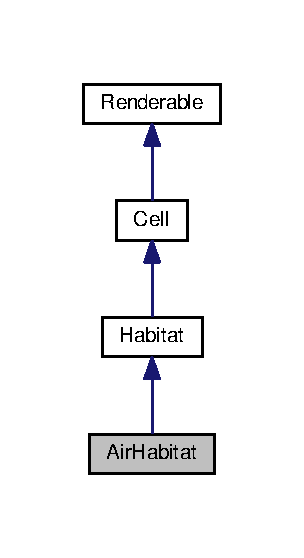
\includegraphics[width=146pt]{classAirHabitat__inherit__graph}
\end{center}
\end{figure}


Collaboration diagram for Air\+Habitat\+:
\nopagebreak
\begin{figure}[H]
\begin{center}
\leavevmode
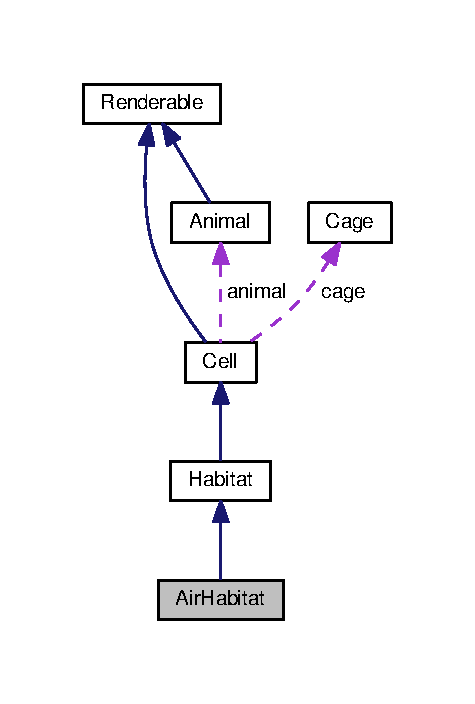
\includegraphics[width=228pt]{classAirHabitat__coll__graph}
\end{center}
\end{figure}
\subsection*{Public Member Functions}
\begin{DoxyCompactItemize}
\item 
\hyperlink{classAirHabitat_ab17317e1cca06d76389eb65b084bf37b}{Air\+Habitat} (int x, int y)
\begin{DoxyCompactList}\small\item\em Constructor Menciptakan \hyperlink{classAirHabitat}{Air\+Habitat} dengan memanggil constructor \hyperlink{classHabitat}{Habitat} bertype \textquotesingle{}o\textquotesingle{}, dan posisi $<$x,y$>$ \end{DoxyCompactList}\end{DoxyCompactItemize}
\subsection*{Additional Inherited Members}


\subsection{Detailed Description}
Kelas \hyperlink{classAirHabitat}{Air\+Habitat} inherit dari kelas \hyperlink{classHabitat}{Habitat} tempat hewan yang hidup di udara 

\subsection{Constructor \& Destructor Documentation}
\index{Air\+Habitat@{Air\+Habitat}!Air\+Habitat@{Air\+Habitat}}
\index{Air\+Habitat@{Air\+Habitat}!Air\+Habitat@{Air\+Habitat}}
\subsubsection[{\texorpdfstring{Air\+Habitat(int x, int y)}{AirHabitat(int x, int y)}}]{\setlength{\rightskip}{0pt plus 5cm}Air\+Habitat\+::\+Air\+Habitat (
\begin{DoxyParamCaption}
\item[{int}]{x, }
\item[{int}]{y}
\end{DoxyParamCaption}
)}\hypertarget{classAirHabitat_ab17317e1cca06d76389eb65b084bf37b}{}\label{classAirHabitat_ab17317e1cca06d76389eb65b084bf37b}


Constructor Menciptakan \hyperlink{classAirHabitat}{Air\+Habitat} dengan memanggil constructor \hyperlink{classHabitat}{Habitat} bertype \textquotesingle{}o\textquotesingle{}, dan posisi $<$x,y$>$ 


\begin{DoxyParams}{Parameters}
{\em x} & Nilai absis \hyperlink{classAirHabitat}{Air\+Habitat} yang diciptakan \\
\hline
{\em y} & Nilai ordinat \hyperlink{classAirHabitat}{Air\+Habitat} yang diciptakan \\
\hline
\end{DoxyParams}


The documentation for this class was generated from the following files\+:\begin{DoxyCompactItemize}
\item 
zoo.\+h\item 
zoo.\+cpp\end{DoxyCompactItemize}

\hypertarget{classAligator}{}\section{Aligator Class Reference}
\label{classAligator}\index{Aligator@{Aligator}}


{\ttfamily \#include $<$listanimal.\+h$>$}



Inheritance diagram for Aligator\+:
\nopagebreak
\begin{figure}[H]
\begin{center}
\leavevmode
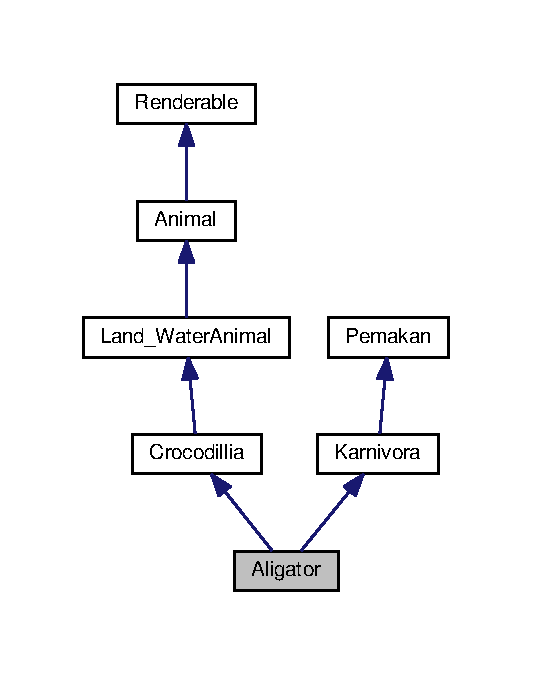
\includegraphics[width=256pt]{classAligator__inherit__graph}
\end{center}
\end{figure}


Collaboration diagram for Aligator\+:
\nopagebreak
\begin{figure}[H]
\begin{center}
\leavevmode
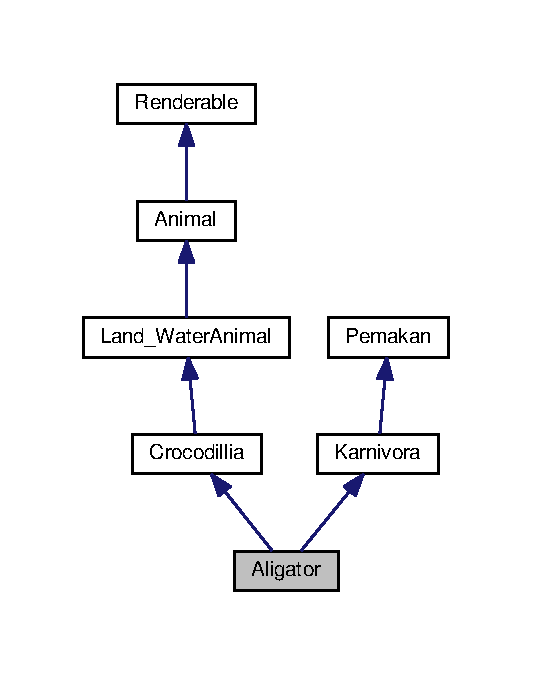
\includegraphics[width=256pt]{classAligator__coll__graph}
\end{center}
\end{figure}
\subsection*{Public Member Functions}
\begin{DoxyCompactItemize}
\item 
\hyperlink{classAligator_a19d0ebd3217864614103b0bbd343a48c}{Aligator} (int i, int x, int y, int massa, bool jinak)
\begin{DoxyCompactList}\small\item\em Constructor. Menciptakan \hyperlink{classRusa}{Rusa} dengan inisial \textquotesingle{}L\textquotesingle{} dan ID i. \end{DoxyCompactList}\item 
void \hyperlink{classAligator_ad314ab524831f78dccd550f545932895}{Interact} ()\hypertarget{classAligator_ad314ab524831f78dccd550f545932895}{}\label{classAligator_ad314ab524831f78dccd550f545932895}

\begin{DoxyCompactList}\small\item\em Menampilkan aksi binatang ke layar. \end{DoxyCompactList}\item 
int \hyperlink{classAligator_a58857a88d44930ecea013d1d71008567}{Get\+Jml\+Makanan} ()
\begin{DoxyCompactList}\small\item\em Melihat jumlah makanan dari binatang. Memanggil fungsi Get\+Amount parent \hyperlink{classKarnivora}{Karnivora}. \end{DoxyCompactList}\end{DoxyCompactItemize}
\subsection*{Additional Inherited Members}


\subsection{Detailed Description}
Kelas \hyperlink{classAligator}{Aligator} turunan dari \hyperlink{classCrocodillia}{Crocodillia} dan \hyperlink{classKarnivora}{Karnivora} 

\subsection{Constructor \& Destructor Documentation}
\index{Aligator@{Aligator}!Aligator@{Aligator}}
\index{Aligator@{Aligator}!Aligator@{Aligator}}
\subsubsection[{\texorpdfstring{Aligator(int i, int x, int y, int massa, bool jinak)}{Aligator(int i, int x, int y, int massa, bool jinak)}}]{\setlength{\rightskip}{0pt plus 5cm}Aligator\+::\+Aligator (
\begin{DoxyParamCaption}
\item[{int}]{i, }
\item[{int}]{x, }
\item[{int}]{y, }
\item[{int}]{massa, }
\item[{bool}]{jinak}
\end{DoxyParamCaption}
)}\hypertarget{classAligator_a19d0ebd3217864614103b0bbd343a48c}{}\label{classAligator_a19d0ebd3217864614103b0bbd343a48c}


Constructor. Menciptakan \hyperlink{classRusa}{Rusa} dengan inisial \textquotesingle{}L\textquotesingle{} dan ID i. 


\begin{DoxyParams}{Parameters}
{\em i} & Nilai Id \hyperlink{classAnimal}{Animal} yang diciptakan \\
\hline
{\em x} & Posisi x \hyperlink{classAnimal}{Animal} yang diciptakan \\
\hline
{\em y} & Posisi y \hyperlink{classAnimal}{Animal} yang diciptakan \\
\hline
{\em massa} & berat \hyperlink{classAnimal}{Animal} yang diciptakan \\
\hline
{\em jinak} & nilai jinak \hyperlink{classAnimal}{Animal} yang diciptakan \\
\hline
\end{DoxyParams}


\subsection{Member Function Documentation}
\index{Aligator@{Aligator}!Get\+Jml\+Makanan@{Get\+Jml\+Makanan}}
\index{Get\+Jml\+Makanan@{Get\+Jml\+Makanan}!Aligator@{Aligator}}
\subsubsection[{\texorpdfstring{Get\+Jml\+Makanan()}{GetJmlMakanan()}}]{\setlength{\rightskip}{0pt plus 5cm}int Aligator\+::\+Get\+Jml\+Makanan (
\begin{DoxyParamCaption}
{}
\end{DoxyParamCaption}
)\hspace{0.3cm}{\ttfamily [virtual]}}\hypertarget{classAligator_a58857a88d44930ecea013d1d71008567}{}\label{classAligator_a58857a88d44930ecea013d1d71008567}


Melihat jumlah makanan dari binatang. Memanggil fungsi Get\+Amount parent \hyperlink{classKarnivora}{Karnivora}. 

\begin{DoxyReturn}{Returns}
Jumlah makanan dari binatang. 
\end{DoxyReturn}


Implements \hyperlink{classAnimal_a3f1cced7bac93f7c88a24ec5a0e989fe}{Animal}.



The documentation for this class was generated from the following files\+:\begin{DoxyCompactItemize}
\item 
listanimal.\+h\item 
listanimal.\+cpp\end{DoxyCompactItemize}

\hypertarget{classAnimal}{}\section{Animal Class Reference}
\label{classAnimal}\index{Animal@{Animal}}


{\ttfamily \#include $<$animal.\+h$>$}



Inheritance diagram for Animal\+:
\nopagebreak
\begin{figure}[H]
\begin{center}
\leavevmode
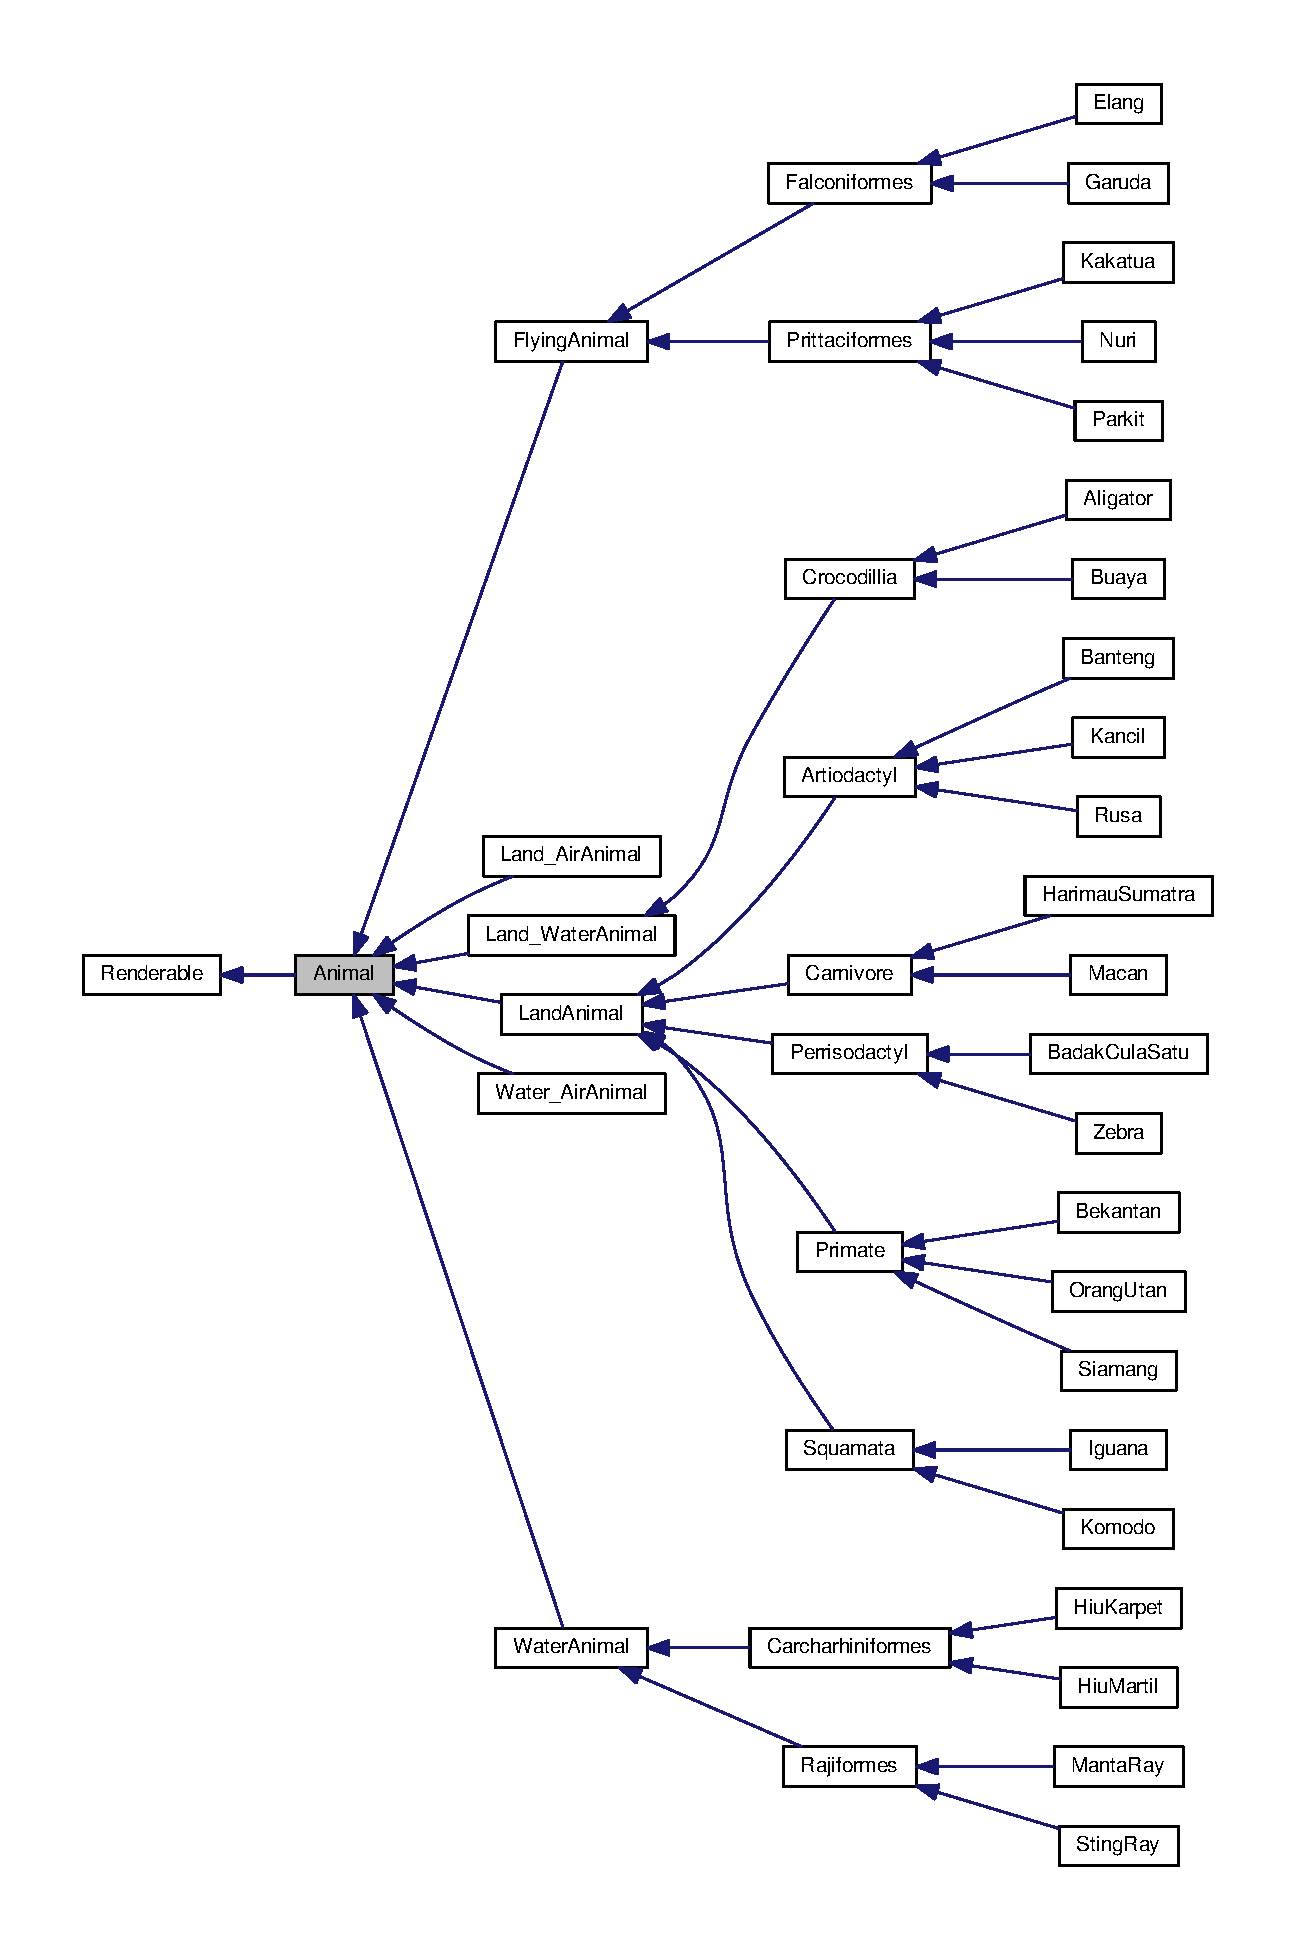
\includegraphics[width=350pt]{classAnimal__inherit__graph}
\end{center}
\end{figure}


Collaboration diagram for Animal\+:
\nopagebreak
\begin{figure}[H]
\begin{center}
\leavevmode
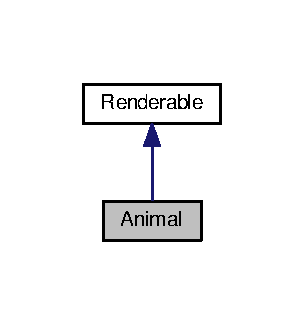
\includegraphics[width=146pt]{classAnimal__coll__graph}
\end{center}
\end{figure}
\subsection*{Public Member Functions}
\begin{DoxyCompactItemize}
\item 
\hyperlink{classAnimal_a57dcbdda5c07d91a7f8fe94da97953fe}{Animal} (char c, int i)
\begin{DoxyCompactList}\small\item\em Constructor. \end{DoxyCompactList}\item 
void \hyperlink{classAnimal_ac6c9fc3c1f84fd9416ed8b584d892d3a}{Set\+Jinak} (bool \+\_\+jinak)
\begin{DoxyCompactList}\small\item\em Setter jinak. \end{DoxyCompactList}\item 
bool \hyperlink{classAnimal_a0068651e223252b68e634714f4e414ca}{Is\+Jinak} ()
\begin{DoxyCompactList}\small\item\em Mengecek apakah animal jinak. \end{DoxyCompactList}\item 
char \hyperlink{classAnimal_a98d6f1e3cbc08c981f7b11ecc5b3886e}{Get\+Inisial} ()
\begin{DoxyCompactList}\small\item\em Getter inisial. \end{DoxyCompactList}\item 
int \hyperlink{classAnimal_abfb32d0af74791999af1e7cebcff575d}{Get\+ID} ()
\begin{DoxyCompactList}\small\item\em Getter ID. \end{DoxyCompactList}\item 
int \hyperlink{classAnimal_a5c05eda69a23388786f54395654ba56f}{Get\+Massa} ()
\begin{DoxyCompactList}\small\item\em Getter massa. \end{DoxyCompactList}\item 
int \hyperlink{classAnimal_abcec270bc5610a32ddd9327847b4c72c}{Get\+PosisiX} ()
\begin{DoxyCompactList}\small\item\em Getter posisi x. \end{DoxyCompactList}\item 
int \hyperlink{classAnimal_a1adc84f7d029ae24c3236ea9ba5d083c}{Get\+PosisiY} ()
\begin{DoxyCompactList}\small\item\em Getter posisi y. \end{DoxyCompactList}\item 
void \hyperlink{classAnimal_aa3fa9d72dbcb5acc7310366d8ff361d5}{Set\+Massa} (int kg)
\begin{DoxyCompactList}\small\item\em Setter massa. \end{DoxyCompactList}\item 
void \hyperlink{classAnimal_ae938862e1651b348b2ed5fcc5b64c625}{SetX} (int \+\_\+x)
\begin{DoxyCompactList}\small\item\em Setter x. \end{DoxyCompactList}\item 
void \hyperlink{classAnimal_af4892ee71e8bbc91f23797ee4dbe3100}{SetY} (int \+\_\+y)
\begin{DoxyCompactList}\small\item\em Setter y. \end{DoxyCompactList}\item 
void \hyperlink{classAnimal_a00c911d660d2a76c6fc696cf6fe26617}{Render} ()\hypertarget{classAnimal_a00c911d660d2a76c6fc696cf6fe26617}{}\label{classAnimal_a00c911d660d2a76c6fc696cf6fe26617}

\begin{DoxyCompactList}\small\item\em Menampilkan karakter inisial dari animal ke layar. \end{DoxyCompactList}\item 
vector$<$ char $>$ \& \hyperlink{classAnimal_a892a7fc299149570c841ee7215b4bb4b}{Get\+Habitat} ()
\begin{DoxyCompactList}\small\item\em Getter type. \end{DoxyCompactList}\item 
void \hyperlink{classAnimal_a8a40826811fda32a7a3dfeae6b8723fd}{Add\+Habitat} (char c)
\begin{DoxyCompactList}\small\item\em Menambahkan c kedalam type. \end{DoxyCompactList}\item 
virtual int \hyperlink{classAnimal_a3f1cced7bac93f7c88a24ec5a0e989fe}{Get\+Jml\+Makanan} ()=0
\begin{DoxyCompactList}\small\item\em Getter jumlah makanan animal. \end{DoxyCompactList}\item 
virtual void \hyperlink{classAnimal_aa620e55ec419fc9b20d983d933b5ee11}{Interact} ()=0\hypertarget{classAnimal_aa620e55ec419fc9b20d983d933b5ee11}{}\label{classAnimal_aa620e55ec419fc9b20d983d933b5ee11}

\begin{DoxyCompactList}\small\item\em Menampilkan interaksi dari animal Menampilkan interaksi animal ke layar. \end{DoxyCompactList}\end{DoxyCompactItemize}
\subsection*{Additional Inherited Members}


\subsection{Detailed Description}
Kelas \hyperlink{classAnimal}{Animal} representasi binatang dengan posisi, massa dan ketentuan jinak. 

\subsection{Constructor \& Destructor Documentation}
\index{Animal@{Animal}!Animal@{Animal}}
\index{Animal@{Animal}!Animal@{Animal}}
\subsubsection[{\texorpdfstring{Animal(char c, int i)}{Animal(char c, int i)}}]{\setlength{\rightskip}{0pt plus 5cm}Animal\+::\+Animal (
\begin{DoxyParamCaption}
\item[{char}]{c, }
\item[{int}]{i}
\end{DoxyParamCaption}
)}\hypertarget{classAnimal_a57dcbdda5c07d91a7f8fe94da97953fe}{}\label{classAnimal_a57dcbdda5c07d91a7f8fe94da97953fe}


Constructor. 


\begin{DoxyParams}{Parameters}
{\em c} & Nilai inisial \hyperlink{classAnimal}{Animal} yang ingin diciptakan \\
\hline
{\em i} & Nilai ID \hyperlink{classAnimal}{Animal} yang ingin diciptakan \\
\hline
\end{DoxyParams}


\subsection{Member Function Documentation}
\index{Animal@{Animal}!Add\+Habitat@{Add\+Habitat}}
\index{Add\+Habitat@{Add\+Habitat}!Animal@{Animal}}
\subsubsection[{\texorpdfstring{Add\+Habitat(char c)}{AddHabitat(char c)}}]{\setlength{\rightskip}{0pt plus 5cm}void Animal\+::\+Add\+Habitat (
\begin{DoxyParamCaption}
\item[{char}]{c}
\end{DoxyParamCaption}
)}\hypertarget{classAnimal_a8a40826811fda32a7a3dfeae6b8723fd}{}\label{classAnimal_a8a40826811fda32a7a3dfeae6b8723fd}


Menambahkan c kedalam type. 


\begin{DoxyParams}{Parameters}
{\em c} & nilai habitat animal yang ingin ditambahkan ke type \\
\hline
\end{DoxyParams}
\index{Animal@{Animal}!Get\+Habitat@{Get\+Habitat}}
\index{Get\+Habitat@{Get\+Habitat}!Animal@{Animal}}
\subsubsection[{\texorpdfstring{Get\+Habitat()}{GetHabitat()}}]{\setlength{\rightskip}{0pt plus 5cm}vector$<$ char $>$ \& Animal\+::\+Get\+Habitat (
\begin{DoxyParamCaption}
{}
\end{DoxyParamCaption}
)}\hypertarget{classAnimal_a892a7fc299149570c841ee7215b4bb4b}{}\label{classAnimal_a892a7fc299149570c841ee7215b4bb4b}


Getter type. 

\begin{DoxyReturn}{Returns}
type 
\end{DoxyReturn}
\index{Animal@{Animal}!Get\+ID@{Get\+ID}}
\index{Get\+ID@{Get\+ID}!Animal@{Animal}}
\subsubsection[{\texorpdfstring{Get\+I\+D()}{GetID()}}]{\setlength{\rightskip}{0pt plus 5cm}int Animal\+::\+Get\+ID (
\begin{DoxyParamCaption}
{}
\end{DoxyParamCaption}
)}\hypertarget{classAnimal_abfb32d0af74791999af1e7cebcff575d}{}\label{classAnimal_abfb32d0af74791999af1e7cebcff575d}


Getter ID. 

\begin{DoxyReturn}{Returns}
ID 
\end{DoxyReturn}
\index{Animal@{Animal}!Get\+Inisial@{Get\+Inisial}}
\index{Get\+Inisial@{Get\+Inisial}!Animal@{Animal}}
\subsubsection[{\texorpdfstring{Get\+Inisial()}{GetInisial()}}]{\setlength{\rightskip}{0pt plus 5cm}char Animal\+::\+Get\+Inisial (
\begin{DoxyParamCaption}
{}
\end{DoxyParamCaption}
)}\hypertarget{classAnimal_a98d6f1e3cbc08c981f7b11ecc5b3886e}{}\label{classAnimal_a98d6f1e3cbc08c981f7b11ecc5b3886e}


Getter inisial. 

\begin{DoxyReturn}{Returns}
inisial 
\end{DoxyReturn}
\index{Animal@{Animal}!Get\+Jml\+Makanan@{Get\+Jml\+Makanan}}
\index{Get\+Jml\+Makanan@{Get\+Jml\+Makanan}!Animal@{Animal}}
\subsubsection[{\texorpdfstring{Get\+Jml\+Makanan()=0}{GetJmlMakanan()=0}}]{\setlength{\rightskip}{0pt plus 5cm}virtual int Animal\+::\+Get\+Jml\+Makanan (
\begin{DoxyParamCaption}
{}
\end{DoxyParamCaption}
)\hspace{0.3cm}{\ttfamily [pure virtual]}}\hypertarget{classAnimal_a3f1cced7bac93f7c88a24ec5a0e989fe}{}\label{classAnimal_a3f1cced7bac93f7c88a24ec5a0e989fe}


Getter jumlah makanan animal. 

\begin{DoxyReturn}{Returns}
Nilai makanan yang diperlukan animal 
\end{DoxyReturn}


Implemented in \hyperlink{classAligator_a58857a88d44930ecea013d1d71008567}{Aligator}, \hyperlink{classBuaya_a00f50933adea8ab884443d344f388bfb}{Buaya}, \hyperlink{classParkit_a2c4755adea1478b458052fe975e212dc}{Parkit}, \hyperlink{classNuri_ac3bacc743d41a816b8852efe0d2b221c}{Nuri}, \hyperlink{classKakatua_a981115d43e229e2516227e9919286133}{Kakatua}, \hyperlink{classGaruda_a66653e83dc102c16d2a8c99cad247075}{Garuda}, \hyperlink{classElang_a6d017711dba92202dfad0126d636a28a}{Elang}, \hyperlink{classMantaRay_a1bd6cf276ee3033d181f6b91297da09e}{Manta\+Ray}, \hyperlink{classStingRay_aa1c718c7a2d420cdeac49df66c17ae07}{Sting\+Ray}, \hyperlink{classHiuMartil_a8b643c318a9b69730c26a73b268f0b2c}{Hiu\+Martil}, \hyperlink{classHiuKarpet_abcb51ba250304ab5b9a0a649c1e705d1}{Hiu\+Karpet}, \hyperlink{classIguana_ae871a38dfe31ebba979268ba881cff1a}{Iguana}, \hyperlink{classKomodo_a308c3080f48dc07b8cf9374fd2aa9d0d}{Komodo}, \hyperlink{classBanteng_a302f2f5b3eaf114afedef16c9d5d129f}{Banteng}, \hyperlink{classKancil_ab958e9fa65f83d505aaba333b4119790}{Kancil}, \hyperlink{classRusa_aafe45dbc124b4639bee4d625a7461d1b}{Rusa}, \hyperlink{classMacan_a8e8ce4a0d08de3b41b6f669dd23b207a}{Macan}, \hyperlink{classHarimauSumatra_a26c0ee52d2f214027e9998aeef3646e5}{Harimau\+Sumatra}, \hyperlink{classZebra_a1ad885f1ff84bfea442a330fea7c6eaa}{Zebra}, \hyperlink{classBadakCulaSatu_a1b53ef7e5a7fbcb46c9daffc3be05bfb}{Badak\+Cula\+Satu}, \hyperlink{classBekantan_a84c8ea3d97bd95d0c108d4016b5be934}{Bekantan}, \hyperlink{classSiamang_af604ba0243bb13132d2b5ac191f41839}{Siamang}, and \hyperlink{classOrangUtan_ac1e2890d346b10b9235e1ee2f8d22d79}{Orang\+Utan}.

\index{Animal@{Animal}!Get\+Massa@{Get\+Massa}}
\index{Get\+Massa@{Get\+Massa}!Animal@{Animal}}
\subsubsection[{\texorpdfstring{Get\+Massa()}{GetMassa()}}]{\setlength{\rightskip}{0pt plus 5cm}int Animal\+::\+Get\+Massa (
\begin{DoxyParamCaption}
{}
\end{DoxyParamCaption}
)}\hypertarget{classAnimal_a5c05eda69a23388786f54395654ba56f}{}\label{classAnimal_a5c05eda69a23388786f54395654ba56f}


Getter massa. 

\begin{DoxyReturn}{Returns}
massa 
\end{DoxyReturn}
\index{Animal@{Animal}!Get\+PosisiX@{Get\+PosisiX}}
\index{Get\+PosisiX@{Get\+PosisiX}!Animal@{Animal}}
\subsubsection[{\texorpdfstring{Get\+Posisi\+X()}{GetPosisiX()}}]{\setlength{\rightskip}{0pt plus 5cm}int Animal\+::\+Get\+PosisiX (
\begin{DoxyParamCaption}
{}
\end{DoxyParamCaption}
)}\hypertarget{classAnimal_abcec270bc5610a32ddd9327847b4c72c}{}\label{classAnimal_abcec270bc5610a32ddd9327847b4c72c}


Getter posisi x. 

\begin{DoxyReturn}{Returns}
x 
\end{DoxyReturn}
\index{Animal@{Animal}!Get\+PosisiY@{Get\+PosisiY}}
\index{Get\+PosisiY@{Get\+PosisiY}!Animal@{Animal}}
\subsubsection[{\texorpdfstring{Get\+Posisi\+Y()}{GetPosisiY()}}]{\setlength{\rightskip}{0pt plus 5cm}int Animal\+::\+Get\+PosisiY (
\begin{DoxyParamCaption}
{}
\end{DoxyParamCaption}
)}\hypertarget{classAnimal_a1adc84f7d029ae24c3236ea9ba5d083c}{}\label{classAnimal_a1adc84f7d029ae24c3236ea9ba5d083c}


Getter posisi y. 

\begin{DoxyReturn}{Returns}
y 
\end{DoxyReturn}
\index{Animal@{Animal}!Is\+Jinak@{Is\+Jinak}}
\index{Is\+Jinak@{Is\+Jinak}!Animal@{Animal}}
\subsubsection[{\texorpdfstring{Is\+Jinak()}{IsJinak()}}]{\setlength{\rightskip}{0pt plus 5cm}bool Animal\+::\+Is\+Jinak (
\begin{DoxyParamCaption}
{}
\end{DoxyParamCaption}
)}\hypertarget{classAnimal_a0068651e223252b68e634714f4e414ca}{}\label{classAnimal_a0068651e223252b68e634714f4e414ca}


Mengecek apakah animal jinak. 

\begin{DoxyReturn}{Returns}
jinak 
\end{DoxyReturn}
\index{Animal@{Animal}!Set\+Jinak@{Set\+Jinak}}
\index{Set\+Jinak@{Set\+Jinak}!Animal@{Animal}}
\subsubsection[{\texorpdfstring{Set\+Jinak(bool \+\_\+jinak)}{SetJinak(bool _jinak)}}]{\setlength{\rightskip}{0pt plus 5cm}void Animal\+::\+Set\+Jinak (
\begin{DoxyParamCaption}
\item[{bool}]{\+\_\+jinak}
\end{DoxyParamCaption}
)}\hypertarget{classAnimal_ac6c9fc3c1f84fd9416ed8b584d892d3a}{}\label{classAnimal_ac6c9fc3c1f84fd9416ed8b584d892d3a}


Setter jinak. 


\begin{DoxyParams}{Parameters}
{\em \+\_\+jinak} & Nilai jinak \hyperlink{classAnimal}{Animal} yang ingin dimasukkan \\
\hline
\end{DoxyParams}
\index{Animal@{Animal}!Set\+Massa@{Set\+Massa}}
\index{Set\+Massa@{Set\+Massa}!Animal@{Animal}}
\subsubsection[{\texorpdfstring{Set\+Massa(int kg)}{SetMassa(int kg)}}]{\setlength{\rightskip}{0pt plus 5cm}void Animal\+::\+Set\+Massa (
\begin{DoxyParamCaption}
\item[{int}]{kg}
\end{DoxyParamCaption}
)}\hypertarget{classAnimal_aa3fa9d72dbcb5acc7310366d8ff361d5}{}\label{classAnimal_aa3fa9d72dbcb5acc7310366d8ff361d5}


Setter massa. 


\begin{DoxyParams}{Parameters}
{\em kg} & Nilai massa animal yang ingin dimasukkan \\
\hline
\end{DoxyParams}
\index{Animal@{Animal}!SetX@{SetX}}
\index{SetX@{SetX}!Animal@{Animal}}
\subsubsection[{\texorpdfstring{Set\+X(int \+\_\+x)}{SetX(int _x)}}]{\setlength{\rightskip}{0pt plus 5cm}void Animal\+::\+SetX (
\begin{DoxyParamCaption}
\item[{int}]{\+\_\+x}
\end{DoxyParamCaption}
)}\hypertarget{classAnimal_ae938862e1651b348b2ed5fcc5b64c625}{}\label{classAnimal_ae938862e1651b348b2ed5fcc5b64c625}


Setter x. 


\begin{DoxyParams}{Parameters}
{\em \+\_\+x} & Nilai posisi x animal yang ingin dimasukkan \\
\hline
\end{DoxyParams}
\index{Animal@{Animal}!SetY@{SetY}}
\index{SetY@{SetY}!Animal@{Animal}}
\subsubsection[{\texorpdfstring{Set\+Y(int \+\_\+y)}{SetY(int _y)}}]{\setlength{\rightskip}{0pt plus 5cm}void Animal\+::\+SetY (
\begin{DoxyParamCaption}
\item[{int}]{\+\_\+y}
\end{DoxyParamCaption}
)}\hypertarget{classAnimal_af4892ee71e8bbc91f23797ee4dbe3100}{}\label{classAnimal_af4892ee71e8bbc91f23797ee4dbe3100}


Setter y. 


\begin{DoxyParams}{Parameters}
{\em \+\_\+y} & Nilai posisi y animal yang ingin dimasukkan \\
\hline
\end{DoxyParams}


The documentation for this class was generated from the following files\+:\begin{DoxyCompactItemize}
\item 
animal.\+h\item 
animal.\+cpp\end{DoxyCompactItemize}

\hypertarget{classAnimalHandler}{}\section{Animal\+Handler Class Reference}
\label{classAnimalHandler}\index{Animal\+Handler@{Animal\+Handler}}


{\ttfamily \#include $<$animal.\+h$>$}

\subsection*{Public Member Functions}
\begin{DoxyCompactItemize}
\item 
\hyperlink{classAnimalHandler_a53551d20027ea45c16e05e50cc105d3c}{Animal\+Handler} ()\hypertarget{classAnimalHandler_a53551d20027ea45c16e05e50cc105d3c}{}\label{classAnimalHandler_a53551d20027ea45c16e05e50cc105d3c}

\begin{DoxyCompactList}\small\item\em Constructor. inisiasi n dengan 0. \end{DoxyCompactList}\item 
\hyperlink{classAnimalHandler_a37b9bbd41298a75ade76cf0bc787ee92}{$\sim$\+Animal\+Handler} ()\hypertarget{classAnimalHandler_a37b9bbd41298a75ade76cf0bc787ee92}{}\label{classAnimalHandler_a37b9bbd41298a75ade76cf0bc787ee92}

\begin{DoxyCompactList}\small\item\em Destructor. \end{DoxyCompactList}\item 
\hyperlink{classAnimal}{Animal} $\ast$ \hyperlink{classAnimalHandler_a5484cd394f30786259aa93ba3c88bfce}{Get\+Animal} (int id)
\begin{DoxyCompactList}\small\item\em Getter elemen animal. \end{DoxyCompactList}\item 
int \hyperlink{classAnimalHandler_a5254f930160c47370c5f226c996cec2d}{Nb\+Animal} ()
\begin{DoxyCompactList}\small\item\em Mengetahui jumlah animal. \end{DoxyCompactList}\item 
void \hyperlink{classAnimalHandler_a5d85a87f7aac6373839018a2ff67b648}{Add\+Animal} (\hyperlink{classAnimal}{Animal} $\ast$a)
\begin{DoxyCompactList}\small\item\em Menambahkan animal kedalam list\+\_\+animal. \end{DoxyCompactList}\item 
int \hyperlink{classAnimalHandler_a3df3838f7ce62e0befef35dd57b18164}{Jumlah\+Makanan} ()
\begin{DoxyCompactList}\small\item\em Mengembalikan jumlah makanan dari seluruh animal Mengiterasi list\+\_\+animal dan menjumlahkan makanan dari tiap animal. \end{DoxyCompactList}\end{DoxyCompactItemize}


\subsection{Detailed Description}
Kelas \hyperlink{classAnimalHandler}{Animal\+Handler} terdiri atas list animal yang pernah diciptakan 

\subsection{Member Function Documentation}
\index{Animal\+Handler@{Animal\+Handler}!Add\+Animal@{Add\+Animal}}
\index{Add\+Animal@{Add\+Animal}!Animal\+Handler@{Animal\+Handler}}
\subsubsection[{\texorpdfstring{Add\+Animal(\+Animal $\ast$a)}{AddAnimal(Animal *a)}}]{\setlength{\rightskip}{0pt plus 5cm}void Animal\+Handler\+::\+Add\+Animal (
\begin{DoxyParamCaption}
\item[{{\bf Animal} $\ast$}]{a}
\end{DoxyParamCaption}
)}\hypertarget{classAnimalHandler_a5d85a87f7aac6373839018a2ff67b648}{}\label{classAnimalHandler_a5d85a87f7aac6373839018a2ff67b648}


Menambahkan animal kedalam list\+\_\+animal. 


\begin{DoxyParams}{Parameters}
{\em a} & \hyperlink{classAnimal}{Animal} yang ingin ditambahkan ke list\+\_\+animal \\
\hline
\end{DoxyParams}
\index{Animal\+Handler@{Animal\+Handler}!Get\+Animal@{Get\+Animal}}
\index{Get\+Animal@{Get\+Animal}!Animal\+Handler@{Animal\+Handler}}
\subsubsection[{\texorpdfstring{Get\+Animal(int id)}{GetAnimal(int id)}}]{\setlength{\rightskip}{0pt plus 5cm}{\bf Animal} $\ast$ Animal\+Handler\+::\+Get\+Animal (
\begin{DoxyParamCaption}
\item[{int}]{id}
\end{DoxyParamCaption}
)}\hypertarget{classAnimalHandler_a5484cd394f30786259aa93ba3c88bfce}{}\label{classAnimalHandler_a5484cd394f30786259aa93ba3c88bfce}


Getter elemen animal. 


\begin{DoxyParams}{Parameters}
{\em id} & nilai id animal yang ingin diketahui \\
\hline
\end{DoxyParams}
\begin{DoxyReturn}{Returns}
animalist\mbox{[}id\mbox{]} 
\end{DoxyReturn}
\index{Animal\+Handler@{Animal\+Handler}!Jumlah\+Makanan@{Jumlah\+Makanan}}
\index{Jumlah\+Makanan@{Jumlah\+Makanan}!Animal\+Handler@{Animal\+Handler}}
\subsubsection[{\texorpdfstring{Jumlah\+Makanan()}{JumlahMakanan()}}]{\setlength{\rightskip}{0pt plus 5cm}int Animal\+Handler\+::\+Jumlah\+Makanan (
\begin{DoxyParamCaption}
{}
\end{DoxyParamCaption}
)}\hypertarget{classAnimalHandler_a3df3838f7ce62e0befef35dd57b18164}{}\label{classAnimalHandler_a3df3838f7ce62e0befef35dd57b18164}


Mengembalikan jumlah makanan dari seluruh animal Mengiterasi list\+\_\+animal dan menjumlahkan makanan dari tiap animal. 

\begin{DoxyReturn}{Returns}
jumlah makanan dari seluruh animal 
\end{DoxyReturn}
\index{Animal\+Handler@{Animal\+Handler}!Nb\+Animal@{Nb\+Animal}}
\index{Nb\+Animal@{Nb\+Animal}!Animal\+Handler@{Animal\+Handler}}
\subsubsection[{\texorpdfstring{Nb\+Animal()}{NbAnimal()}}]{\setlength{\rightskip}{0pt plus 5cm}int Animal\+Handler\+::\+Nb\+Animal (
\begin{DoxyParamCaption}
{}
\end{DoxyParamCaption}
)}\hypertarget{classAnimalHandler_a5254f930160c47370c5f226c996cec2d}{}\label{classAnimalHandler_a5254f930160c47370c5f226c996cec2d}


Mengetahui jumlah animal. 

\begin{DoxyReturn}{Returns}
n 
\end{DoxyReturn}


The documentation for this class was generated from the following files\+:\begin{DoxyCompactItemize}
\item 
animal.\+h\item 
animal.\+cpp\end{DoxyCompactItemize}

\hypertarget{classArtiodactyl}{}\section{Artiodactyl Class Reference}
\label{classArtiodactyl}\index{Artiodactyl@{Artiodactyl}}


{\ttfamily \#include $<$animal.\+h$>$}



Inheritance diagram for Artiodactyl\+:
\nopagebreak
\begin{figure}[H]
\begin{center}
\leavevmode
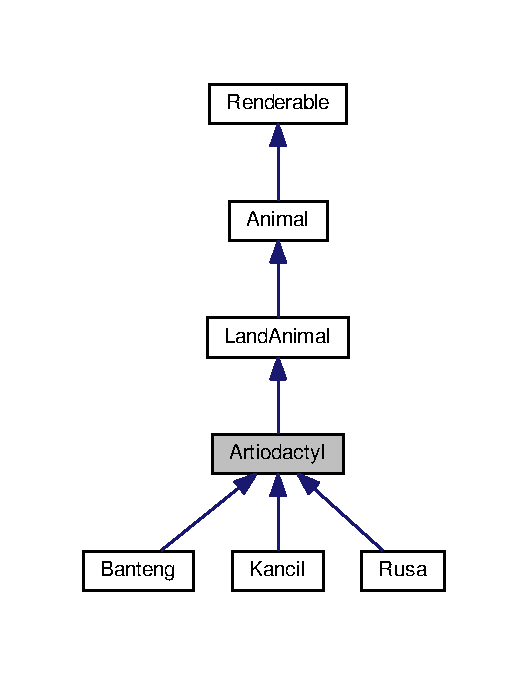
\includegraphics[width=254pt]{classArtiodactyl__inherit__graph}
\end{center}
\end{figure}


Collaboration diagram for Artiodactyl\+:
\nopagebreak
\begin{figure}[H]
\begin{center}
\leavevmode
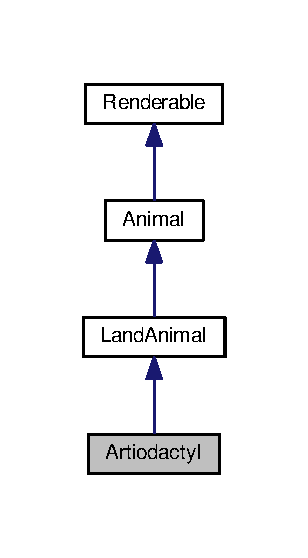
\includegraphics[width=148pt]{classArtiodactyl__coll__graph}
\end{center}
\end{figure}
\subsection*{Public Member Functions}
\begin{DoxyCompactItemize}
\item 
\hyperlink{classArtiodactyl_ab371eaea73e54815518828cdc8a43c8a}{Artiodactyl} (char c, int i)
\begin{DoxyCompactList}\small\item\em Constructor. Menciptakan \hyperlink{classArtiodactyl}{Artiodactyl} dengan memanggil constructor \hyperlink{classLandAnimal}{Land\+Animal} berinisial c dan ID i. \end{DoxyCompactList}\end{DoxyCompactItemize}
\subsection*{Additional Inherited Members}


\subsection{Detailed Description}
Kelas \hyperlink{classArtiodactyl}{Artiodactyl} turunan dari \hyperlink{classLandAnimal}{Land\+Animal} menunjukkan ordo artiodactyl yaitu hewan dengan kuku genap 

\subsection{Constructor \& Destructor Documentation}
\index{Artiodactyl@{Artiodactyl}!Artiodactyl@{Artiodactyl}}
\index{Artiodactyl@{Artiodactyl}!Artiodactyl@{Artiodactyl}}
\subsubsection[{\texorpdfstring{Artiodactyl(char c, int i)}{Artiodactyl(char c, int i)}}]{\setlength{\rightskip}{0pt plus 5cm}Artiodactyl\+::\+Artiodactyl (
\begin{DoxyParamCaption}
\item[{char}]{c, }
\item[{int}]{i}
\end{DoxyParamCaption}
)}\hypertarget{classArtiodactyl_ab371eaea73e54815518828cdc8a43c8a}{}\label{classArtiodactyl_ab371eaea73e54815518828cdc8a43c8a}


Constructor. Menciptakan \hyperlink{classArtiodactyl}{Artiodactyl} dengan memanggil constructor \hyperlink{classLandAnimal}{Land\+Animal} berinisial c dan ID i. 


\begin{DoxyParams}{Parameters}
{\em c} & inisial \hyperlink{classArtiodactyl}{Artiodactyl} yang ingin diciptakan \\
\hline
{\em i} & ID \hyperlink{classArtiodactyl}{Artiodactyl} yang ingin diciptakan \\
\hline
\end{DoxyParams}


The documentation for this class was generated from the following files\+:\begin{DoxyCompactItemize}
\item 
animal.\+h\item 
animal.\+cpp\end{DoxyCompactItemize}

\hypertarget{classBadakCulaSatu}{}\section{Badak\+Cula\+Satu Class Reference}
\label{classBadakCulaSatu}\index{Badak\+Cula\+Satu@{Badak\+Cula\+Satu}}


{\ttfamily \#include $<$listanimal.\+h$>$}



Inheritance diagram for Badak\+Cula\+Satu\+:
\nopagebreak
\begin{figure}[H]
\begin{center}
\leavevmode
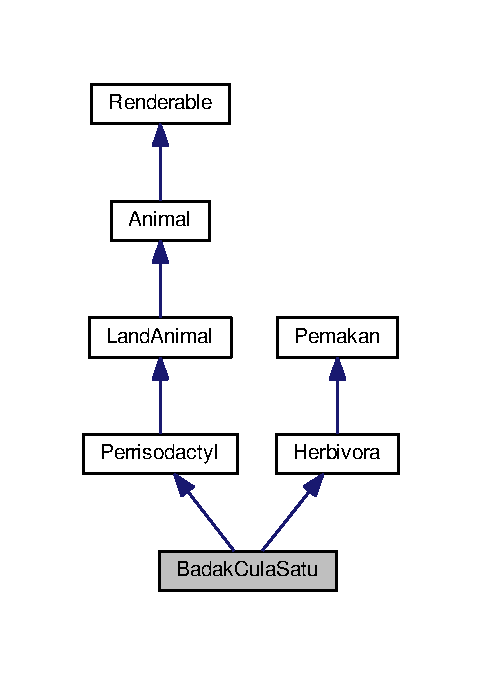
\includegraphics[width=232pt]{classBadakCulaSatu__inherit__graph}
\end{center}
\end{figure}


Collaboration diagram for Badak\+Cula\+Satu\+:
\nopagebreak
\begin{figure}[H]
\begin{center}
\leavevmode
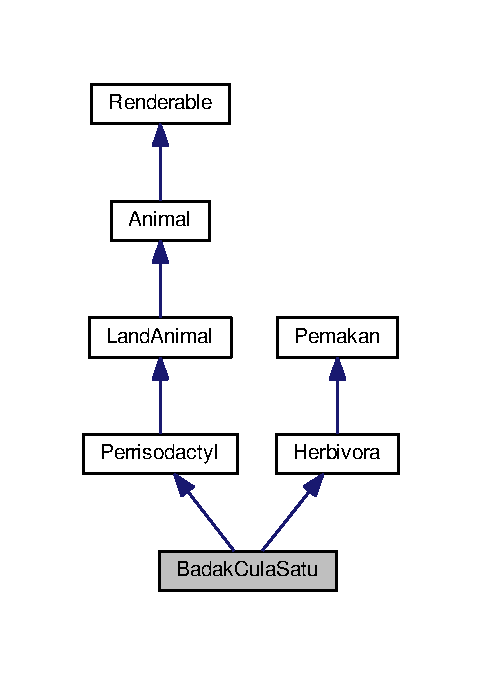
\includegraphics[width=232pt]{classBadakCulaSatu__coll__graph}
\end{center}
\end{figure}
\subsection*{Public Member Functions}
\begin{DoxyCompactItemize}
\item 
\hyperlink{classBadakCulaSatu_acb72f5690f5c5a73e75a76b1cf40dcdc}{Badak\+Cula\+Satu} (int i, int x, int y, int massa, bool jinak)
\begin{DoxyCompactList}\small\item\em Constructor. Menciptakan \hyperlink{classBadakCulaSatu}{Badak\+Cula\+Satu} dengan inisial \textquotesingle{}C\textquotesingle{} dan ID i. \end{DoxyCompactList}\item 
void \hyperlink{classBadakCulaSatu_acf58879822c89caa0d2d873fae9d6538}{Interact} ()\hypertarget{classBadakCulaSatu_acf58879822c89caa0d2d873fae9d6538}{}\label{classBadakCulaSatu_acf58879822c89caa0d2d873fae9d6538}

\begin{DoxyCompactList}\small\item\em Menampilkan aksi binatang ke layar. \end{DoxyCompactList}\item 
int \hyperlink{classBadakCulaSatu_a1b53ef7e5a7fbcb46c9daffc3be05bfb}{Get\+Jml\+Makanan} ()
\begin{DoxyCompactList}\small\item\em Melihat jumlah makanan dari binatang. Memanggil fungsi Get\+Amount parent \hyperlink{classHerbivora}{Herbivora}. \end{DoxyCompactList}\end{DoxyCompactItemize}
\subsection*{Additional Inherited Members}


\subsection{Detailed Description}
Kelas \hyperlink{classBadakCulaSatu}{Badak\+Cula\+Satu} turunan dari \hyperlink{classPerrisodactyl}{Perrisodactyl} dan \hyperlink{classHerbivora}{Herbivora} 

\subsection{Constructor \& Destructor Documentation}
\index{Badak\+Cula\+Satu@{Badak\+Cula\+Satu}!Badak\+Cula\+Satu@{Badak\+Cula\+Satu}}
\index{Badak\+Cula\+Satu@{Badak\+Cula\+Satu}!Badak\+Cula\+Satu@{Badak\+Cula\+Satu}}
\subsubsection[{\texorpdfstring{Badak\+Cula\+Satu(int i, int x, int y, int massa, bool jinak)}{BadakCulaSatu(int i, int x, int y, int massa, bool jinak)}}]{\setlength{\rightskip}{0pt plus 5cm}Badak\+Cula\+Satu\+::\+Badak\+Cula\+Satu (
\begin{DoxyParamCaption}
\item[{int}]{i, }
\item[{int}]{x, }
\item[{int}]{y, }
\item[{int}]{massa, }
\item[{bool}]{jinak}
\end{DoxyParamCaption}
)}\hypertarget{classBadakCulaSatu_acb72f5690f5c5a73e75a76b1cf40dcdc}{}\label{classBadakCulaSatu_acb72f5690f5c5a73e75a76b1cf40dcdc}


Constructor. Menciptakan \hyperlink{classBadakCulaSatu}{Badak\+Cula\+Satu} dengan inisial \textquotesingle{}C\textquotesingle{} dan ID i. 


\begin{DoxyParams}{Parameters}
{\em i} & Nilai Id \hyperlink{classAnimal}{Animal} yang diciptakan \\
\hline
{\em x} & Posisi x \hyperlink{classAnimal}{Animal} yang diciptakan \\
\hline
{\em y} & Posisi y \hyperlink{classAnimal}{Animal} yang diciptakan \\
\hline
{\em massa} & berat \hyperlink{classAnimal}{Animal} yang diciptakan \\
\hline
{\em jinak} & nilai jinak \hyperlink{classAnimal}{Animal} yang diciptakan \\
\hline
\end{DoxyParams}


\subsection{Member Function Documentation}
\index{Badak\+Cula\+Satu@{Badak\+Cula\+Satu}!Get\+Jml\+Makanan@{Get\+Jml\+Makanan}}
\index{Get\+Jml\+Makanan@{Get\+Jml\+Makanan}!Badak\+Cula\+Satu@{Badak\+Cula\+Satu}}
\subsubsection[{\texorpdfstring{Get\+Jml\+Makanan()}{GetJmlMakanan()}}]{\setlength{\rightskip}{0pt plus 5cm}int Badak\+Cula\+Satu\+::\+Get\+Jml\+Makanan (
\begin{DoxyParamCaption}
{}
\end{DoxyParamCaption}
)\hspace{0.3cm}{\ttfamily [virtual]}}\hypertarget{classBadakCulaSatu_a1b53ef7e5a7fbcb46c9daffc3be05bfb}{}\label{classBadakCulaSatu_a1b53ef7e5a7fbcb46c9daffc3be05bfb}


Melihat jumlah makanan dari binatang. Memanggil fungsi Get\+Amount parent \hyperlink{classHerbivora}{Herbivora}. 

\begin{DoxyReturn}{Returns}
Jumlah makanan dari binatang. 
\end{DoxyReturn}


Implements \hyperlink{classAnimal_a3f1cced7bac93f7c88a24ec5a0e989fe}{Animal}.



The documentation for this class was generated from the following files\+:\begin{DoxyCompactItemize}
\item 
listanimal.\+h\item 
listanimal.\+cpp\end{DoxyCompactItemize}

\hypertarget{classBanteng}{}\section{Banteng Class Reference}
\label{classBanteng}\index{Banteng@{Banteng}}


{\ttfamily \#include $<$listanimal.\+h$>$}



Inheritance diagram for Banteng\+:
\nopagebreak
\begin{figure}[H]
\begin{center}
\leavevmode
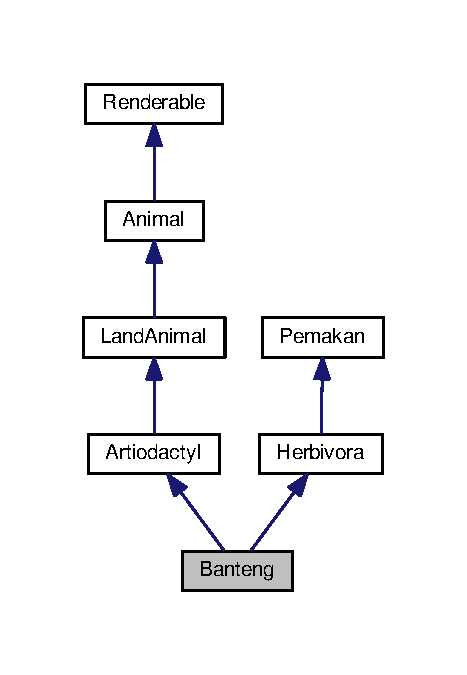
\includegraphics[width=224pt]{classBanteng__inherit__graph}
\end{center}
\end{figure}


Collaboration diagram for Banteng\+:
\nopagebreak
\begin{figure}[H]
\begin{center}
\leavevmode
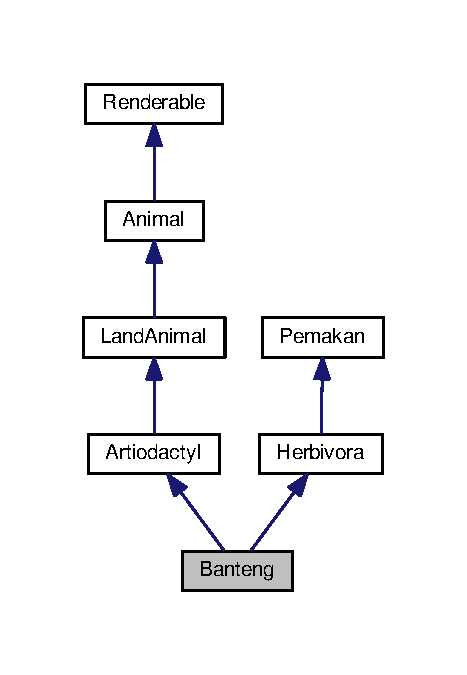
\includegraphics[width=224pt]{classBanteng__coll__graph}
\end{center}
\end{figure}
\subsection*{Public Member Functions}
\begin{DoxyCompactItemize}
\item 
\hyperlink{classBanteng_a67115d9d4b6576dc53668118bcb63284}{Banteng} (int i, int x, int y, int massa, bool jinak)
\begin{DoxyCompactList}\small\item\em Constructor. Menciptakan \hyperlink{classBanteng}{Banteng} dengan inisial \textquotesingle{}A\textquotesingle{} dan ID i. \end{DoxyCompactList}\item 
void \hyperlink{classBanteng_a72cb2d24bcab61fa7c0319211b0d58cf}{Interact} ()\hypertarget{classBanteng_a72cb2d24bcab61fa7c0319211b0d58cf}{}\label{classBanteng_a72cb2d24bcab61fa7c0319211b0d58cf}

\begin{DoxyCompactList}\small\item\em Menampilkan aksi binatang ke layar. \end{DoxyCompactList}\item 
int \hyperlink{classBanteng_a302f2f5b3eaf114afedef16c9d5d129f}{Get\+Jml\+Makanan} ()
\begin{DoxyCompactList}\small\item\em Melihat jumlah makanan dari binatang. Memanggil fungsi Get\+Amount parent \hyperlink{classHerbivora}{Herbivora}. \end{DoxyCompactList}\end{DoxyCompactItemize}
\subsection*{Additional Inherited Members}


\subsection{Detailed Description}
Kelas \hyperlink{classBanteng}{Banteng} turunan dari \hyperlink{classArtiodactyl}{Artiodactyl} dan \hyperlink{classHerbivora}{Herbivora} 

\subsection{Constructor \& Destructor Documentation}
\index{Banteng@{Banteng}!Banteng@{Banteng}}
\index{Banteng@{Banteng}!Banteng@{Banteng}}
\subsubsection[{\texorpdfstring{Banteng(int i, int x, int y, int massa, bool jinak)}{Banteng(int i, int x, int y, int massa, bool jinak)}}]{\setlength{\rightskip}{0pt plus 5cm}Banteng\+::\+Banteng (
\begin{DoxyParamCaption}
\item[{int}]{i, }
\item[{int}]{x, }
\item[{int}]{y, }
\item[{int}]{massa, }
\item[{bool}]{jinak}
\end{DoxyParamCaption}
)}\hypertarget{classBanteng_a67115d9d4b6576dc53668118bcb63284}{}\label{classBanteng_a67115d9d4b6576dc53668118bcb63284}


Constructor. Menciptakan \hyperlink{classBanteng}{Banteng} dengan inisial \textquotesingle{}A\textquotesingle{} dan ID i. 


\begin{DoxyParams}{Parameters}
{\em i} & Nilai Id \hyperlink{classAnimal}{Animal} yang diciptakan \\
\hline
{\em x} & Posisi x \hyperlink{classAnimal}{Animal} yang diciptakan \\
\hline
{\em y} & Posisi y \hyperlink{classAnimal}{Animal} yang diciptakan \\
\hline
{\em massa} & berat \hyperlink{classAnimal}{Animal} yang diciptakan \\
\hline
{\em jinak} & nilai jinak \hyperlink{classAnimal}{Animal} yang diciptakan \\
\hline
\end{DoxyParams}


\subsection{Member Function Documentation}
\index{Banteng@{Banteng}!Get\+Jml\+Makanan@{Get\+Jml\+Makanan}}
\index{Get\+Jml\+Makanan@{Get\+Jml\+Makanan}!Banteng@{Banteng}}
\subsubsection[{\texorpdfstring{Get\+Jml\+Makanan()}{GetJmlMakanan()}}]{\setlength{\rightskip}{0pt plus 5cm}int Banteng\+::\+Get\+Jml\+Makanan (
\begin{DoxyParamCaption}
{}
\end{DoxyParamCaption}
)\hspace{0.3cm}{\ttfamily [virtual]}}\hypertarget{classBanteng_a302f2f5b3eaf114afedef16c9d5d129f}{}\label{classBanteng_a302f2f5b3eaf114afedef16c9d5d129f}


Melihat jumlah makanan dari binatang. Memanggil fungsi Get\+Amount parent \hyperlink{classHerbivora}{Herbivora}. 

\begin{DoxyReturn}{Returns}
Jumlah makanan dari binatang. 
\end{DoxyReturn}


Implements \hyperlink{classAnimal_a3f1cced7bac93f7c88a24ec5a0e989fe}{Animal}.



The documentation for this class was generated from the following files\+:\begin{DoxyCompactItemize}
\item 
listanimal.\+h\item 
listanimal.\+cpp\end{DoxyCompactItemize}

\hypertarget{classnlohmann_1_1basic__json}{}\section{nlohmann\+:\+:basic\+\_\+json$<$ Object\+Type, Array\+Type, String\+Type, Boolean\+Type, Number\+Integer\+Type, Number\+Unsigned\+Type, Number\+Float\+Type, Allocator\+Type, J\+S\+O\+N\+Serializer $>$ Class Template Reference}
\label{classnlohmann_1_1basic__json}\index{nlohmann\+::basic\+\_\+json$<$ Object\+Type, Array\+Type, String\+Type, Boolean\+Type, Number\+Integer\+Type, Number\+Unsigned\+Type, Number\+Float\+Type, Allocator\+Type, J\+S\+O\+N\+Serializer $>$@{nlohmann\+::basic\+\_\+json$<$ Object\+Type, Array\+Type, String\+Type, Boolean\+Type, Number\+Integer\+Type, Number\+Unsigned\+Type, Number\+Float\+Type, Allocator\+Type, J\+S\+O\+N\+Serializer $>$}}


a class to store J\+S\+ON values  




{\ttfamily \#include $<$json.\+hpp$>$}

\subsection*{Classes}
\begin{DoxyCompactItemize}
\item 
class \hyperlink{classnlohmann_1_1basic__json_1_1iter__impl}{iter\+\_\+impl}
\begin{DoxyCompactList}\small\item\em a template for a random access iterator for the \hyperlink{classnlohmann_1_1basic__json}{basic\+\_\+json} class \end{DoxyCompactList}\item 
class \hyperlink{classnlohmann_1_1basic__json_1_1json__pointer}{json\+\_\+pointer}
\begin{DoxyCompactList}\small\item\em J\+S\+ON Pointer. \end{DoxyCompactList}\item 
class \hyperlink{classnlohmann_1_1basic__json_1_1json__reverse__iterator}{json\+\_\+reverse\+\_\+iterator}
\begin{DoxyCompactList}\small\item\em a template for a reverse iterator class \end{DoxyCompactList}\end{DoxyCompactItemize}
\subsection*{Public Types}
\begin{DoxyCompactItemize}
\item 
enum \hyperlink{classnlohmann_1_1basic__json_aea1c863b719b4ca5b77188c171bbfafe}{parse\+\_\+event\+\_\+t} \+: uint8\+\_\+t \{ \\*
\hyperlink{classnlohmann_1_1basic__json_aea1c863b719b4ca5b77188c171bbfafeae73f17027cb0acbb537f29d0a6944b26}{parse\+\_\+event\+\_\+t\+::object\+\_\+start}, 
\hyperlink{classnlohmann_1_1basic__json_aea1c863b719b4ca5b77188c171bbfafeaf63e2a2468a37aa4f394fcc3bcb8249c}{parse\+\_\+event\+\_\+t\+::object\+\_\+end}, 
\hyperlink{classnlohmann_1_1basic__json_aea1c863b719b4ca5b77188c171bbfafeaa4388a3d92419edbb1c6efd4d52461f3}{parse\+\_\+event\+\_\+t\+::array\+\_\+start}, 
\hyperlink{classnlohmann_1_1basic__json_aea1c863b719b4ca5b77188c171bbfafea49642fb732aa2e112188fba1f9d3ef7f}{parse\+\_\+event\+\_\+t\+::array\+\_\+end}, 
\\*
\hyperlink{classnlohmann_1_1basic__json_aea1c863b719b4ca5b77188c171bbfafea3c6e0b8a9c15224a8228b9a98ca1531d}{parse\+\_\+event\+\_\+t\+::key}, 
\hyperlink{classnlohmann_1_1basic__json_aea1c863b719b4ca5b77188c171bbfafea2063c1608d6e0baf80249c42e2be5804}{parse\+\_\+event\+\_\+t\+::value}
 \}\begin{DoxyCompactList}\small\item\em J\+S\+ON callback events. \end{DoxyCompactList}
\item 
using {\bfseries value\+\_\+t} = \hyperlink{namespacenlohmann_1_1detail_a90aa5ef615aa8305e9ea20d8a947980f}{detail\+::value\+\_\+t}\hypertarget{classnlohmann_1_1basic__json_ae8cbef097f7da18a781fc86587de6b90}{}\label{classnlohmann_1_1basic__json_ae8cbef097f7da18a781fc86587de6b90}

\item 
{\footnotesize template$<$typename T , typename S\+F\+I\+N\+AE $>$ }\\using {\bfseries json\+\_\+serializer} = J\+S\+O\+N\+Serializer$<$ T, S\+F\+I\+N\+AE $>$\hypertarget{classnlohmann_1_1basic__json_a7768841baaaa7a21098a401c932efaff}{}\label{classnlohmann_1_1basic__json_a7768841baaaa7a21098a401c932efaff}

\item 
using \hyperlink{classnlohmann_1_1basic__json_aecae491e175f8767c550ae3c59e180e3}{parser\+\_\+callback\+\_\+t} = std\+::function$<$ bool(int depth, \hyperlink{classnlohmann_1_1basic__json_aea1c863b719b4ca5b77188c171bbfafe}{parse\+\_\+event\+\_\+t} event, \hyperlink{classnlohmann_1_1basic__json}{basic\+\_\+json} \&parsed)$>$
\begin{DoxyCompactList}\small\item\em per-\/element parser callback type \end{DoxyCompactList}\end{DoxyCompactItemize}
\subsection*{Public Member Functions}
\begin{DoxyCompactItemize}
\item 
std\+::string \hyperlink{classnlohmann_1_1basic__json_ad6f550a2591b55766603c2c433e2f973}{type\+\_\+name} () const 
\begin{DoxyCompactList}\small\item\em return the type as string \end{DoxyCompactList}\end{DoxyCompactItemize}
\subsection*{Static Public Member Functions}
\begin{DoxyCompactItemize}
\item 
static \hyperlink{classnlohmann_1_1basic__json_a86ce930490cf7773b26f5ef49c04a350}{allocator\+\_\+type} \hyperlink{classnlohmann_1_1basic__json_af4ac14224fbdd29d3547fcb11bb55c8f}{get\+\_\+allocator} ()\hypertarget{classnlohmann_1_1basic__json_af4ac14224fbdd29d3547fcb11bb55c8f}{}\label{classnlohmann_1_1basic__json_af4ac14224fbdd29d3547fcb11bb55c8f}

\begin{DoxyCompactList}\small\item\em returns the allocator associated with the container \end{DoxyCompactList}\item 
static \hyperlink{classnlohmann_1_1basic__json}{basic\+\_\+json} \hyperlink{classnlohmann_1_1basic__json_aef6d0eeccee7c5c7e1317c2ea1607fab}{meta} ()
\begin{DoxyCompactList}\small\item\em returns version information on the library \end{DoxyCompactList}\end{DoxyCompactItemize}
\subsection*{Friends}
\begin{DoxyCompactItemize}
\item 
{\footnotesize template$<$detail\+::value\+\_\+t $>$ }\\struct {\bfseries detail\+::external\+\_\+constructor}\hypertarget{classnlohmann_1_1basic__json_a6275ed57bae6866cdf5db5370a7ad47c}{}\label{classnlohmann_1_1basic__json_a6275ed57bae6866cdf5db5370a7ad47c}

\end{DoxyCompactItemize}
\subsection*{container types}
\label{_amgrp6618fa684bc6d5a05e2c88bfff1c0d66}%
The canonic container types to use \hyperlink{classnlohmann_1_1basic__json}{basic\+\_\+json} like any other S\+TL container. \begin{DoxyCompactItemize}
\item 
using \hyperlink{classnlohmann_1_1basic__json_a2b3297873b70c080837e8eedc4fec32f}{value\+\_\+type} = \hyperlink{classnlohmann_1_1basic__json}{basic\+\_\+json}\hypertarget{classnlohmann_1_1basic__json_a2b3297873b70c080837e8eedc4fec32f}{}\label{classnlohmann_1_1basic__json_a2b3297873b70c080837e8eedc4fec32f}

\begin{DoxyCompactList}\small\item\em the type of elements in a \hyperlink{classnlohmann_1_1basic__json}{basic\+\_\+json} container \end{DoxyCompactList}\item 
using \hyperlink{classnlohmann_1_1basic__json_ac6a5eddd156c776ac75ff54cfe54a5bc}{reference} = \hyperlink{classnlohmann_1_1basic__json_a2b3297873b70c080837e8eedc4fec32f}{value\+\_\+type} \&\hypertarget{classnlohmann_1_1basic__json_ac6a5eddd156c776ac75ff54cfe54a5bc}{}\label{classnlohmann_1_1basic__json_ac6a5eddd156c776ac75ff54cfe54a5bc}

\begin{DoxyCompactList}\small\item\em the type of an element reference \end{DoxyCompactList}\item 
using \hyperlink{classnlohmann_1_1basic__json_a4057c5425f4faacfe39a8046871786ca}{const\+\_\+reference} = const \hyperlink{classnlohmann_1_1basic__json_a2b3297873b70c080837e8eedc4fec32f}{value\+\_\+type} \&\hypertarget{classnlohmann_1_1basic__json_a4057c5425f4faacfe39a8046871786ca}{}\label{classnlohmann_1_1basic__json_a4057c5425f4faacfe39a8046871786ca}

\begin{DoxyCompactList}\small\item\em the type of an element const reference \end{DoxyCompactList}\item 
using \hyperlink{classnlohmann_1_1basic__json_afe7c1303357e19cea9527af4e9a31d8f}{difference\+\_\+type} = std\+::ptrdiff\+\_\+t\hypertarget{classnlohmann_1_1basic__json_afe7c1303357e19cea9527af4e9a31d8f}{}\label{classnlohmann_1_1basic__json_afe7c1303357e19cea9527af4e9a31d8f}

\begin{DoxyCompactList}\small\item\em a type to represent differences between iterators \end{DoxyCompactList}\item 
using \hyperlink{classnlohmann_1_1basic__json_a39f2cd0b58106097e0e67bf185cc519b}{size\+\_\+type} = std\+::size\+\_\+t\hypertarget{classnlohmann_1_1basic__json_a39f2cd0b58106097e0e67bf185cc519b}{}\label{classnlohmann_1_1basic__json_a39f2cd0b58106097e0e67bf185cc519b}

\begin{DoxyCompactList}\small\item\em a type to represent container sizes \end{DoxyCompactList}\item 
using \hyperlink{classnlohmann_1_1basic__json_a86ce930490cf7773b26f5ef49c04a350}{allocator\+\_\+type} = Allocator\+Type$<$ \hyperlink{classnlohmann_1_1basic__json}{basic\+\_\+json} $>$\hypertarget{classnlohmann_1_1basic__json_a86ce930490cf7773b26f5ef49c04a350}{}\label{classnlohmann_1_1basic__json_a86ce930490cf7773b26f5ef49c04a350}

\begin{DoxyCompactList}\small\item\em the allocator type \end{DoxyCompactList}\item 
using \hyperlink{classnlohmann_1_1basic__json_aefee1f777198c68724bd127e0c8abbe4}{pointer} = typename std\+::allocator\+\_\+traits$<$ \hyperlink{classnlohmann_1_1basic__json_a86ce930490cf7773b26f5ef49c04a350}{allocator\+\_\+type} $>$\+::\hyperlink{classnlohmann_1_1basic__json_aefee1f777198c68724bd127e0c8abbe4}{pointer}\hypertarget{classnlohmann_1_1basic__json_aefee1f777198c68724bd127e0c8abbe4}{}\label{classnlohmann_1_1basic__json_aefee1f777198c68724bd127e0c8abbe4}

\begin{DoxyCompactList}\small\item\em the type of an element pointer \end{DoxyCompactList}\item 
using \hyperlink{classnlohmann_1_1basic__json_aff3d5cd2a75612364b888d8693231b58}{const\+\_\+pointer} = typename std\+::allocator\+\_\+traits$<$ \hyperlink{classnlohmann_1_1basic__json_a86ce930490cf7773b26f5ef49c04a350}{allocator\+\_\+type} $>$\+::\hyperlink{classnlohmann_1_1basic__json_aff3d5cd2a75612364b888d8693231b58}{const\+\_\+pointer}\hypertarget{classnlohmann_1_1basic__json_aff3d5cd2a75612364b888d8693231b58}{}\label{classnlohmann_1_1basic__json_aff3d5cd2a75612364b888d8693231b58}

\begin{DoxyCompactList}\small\item\em the type of an element const pointer \end{DoxyCompactList}\item 
using \hyperlink{classnlohmann_1_1basic__json_a099316232c76c034030a38faa6e34dca}{iterator} = \hyperlink{classnlohmann_1_1basic__json_1_1iter__impl}{iter\+\_\+impl}$<$ \hyperlink{classnlohmann_1_1basic__json}{basic\+\_\+json} $>$\hypertarget{classnlohmann_1_1basic__json_a099316232c76c034030a38faa6e34dca}{}\label{classnlohmann_1_1basic__json_a099316232c76c034030a38faa6e34dca}

\begin{DoxyCompactList}\small\item\em an iterator for a \hyperlink{classnlohmann_1_1basic__json}{basic\+\_\+json} container \end{DoxyCompactList}\item 
using \hyperlink{classnlohmann_1_1basic__json_a41a70cf9993951836d129bb1c2b3126a}{const\+\_\+iterator} = \hyperlink{classnlohmann_1_1basic__json_1_1iter__impl}{iter\+\_\+impl}$<$ const \hyperlink{classnlohmann_1_1basic__json}{basic\+\_\+json} $>$\hypertarget{classnlohmann_1_1basic__json_a41a70cf9993951836d129bb1c2b3126a}{}\label{classnlohmann_1_1basic__json_a41a70cf9993951836d129bb1c2b3126a}

\begin{DoxyCompactList}\small\item\em a const iterator for a \hyperlink{classnlohmann_1_1basic__json}{basic\+\_\+json} container \end{DoxyCompactList}\item 
using \hyperlink{classnlohmann_1_1basic__json_ac223d5560c2b05a208c88de67376c5f2}{reverse\+\_\+iterator} = \hyperlink{classnlohmann_1_1basic__json_1_1json__reverse__iterator}{json\+\_\+reverse\+\_\+iterator}$<$ typename \hyperlink{classnlohmann_1_1basic__json_a099316232c76c034030a38faa6e34dca}{basic\+\_\+json\+::iterator} $>$\hypertarget{classnlohmann_1_1basic__json_ac223d5560c2b05a208c88de67376c5f2}{}\label{classnlohmann_1_1basic__json_ac223d5560c2b05a208c88de67376c5f2}

\begin{DoxyCompactList}\small\item\em a reverse iterator for a \hyperlink{classnlohmann_1_1basic__json}{basic\+\_\+json} container \end{DoxyCompactList}\item 
using \hyperlink{classnlohmann_1_1basic__json_a72be3c24bfa24f0993d6c11af03e7404}{const\+\_\+reverse\+\_\+iterator} = \hyperlink{classnlohmann_1_1basic__json_1_1json__reverse__iterator}{json\+\_\+reverse\+\_\+iterator}$<$ typename \hyperlink{classnlohmann_1_1basic__json_a41a70cf9993951836d129bb1c2b3126a}{basic\+\_\+json\+::const\+\_\+iterator} $>$\hypertarget{classnlohmann_1_1basic__json_a72be3c24bfa24f0993d6c11af03e7404}{}\label{classnlohmann_1_1basic__json_a72be3c24bfa24f0993d6c11af03e7404}

\begin{DoxyCompactList}\small\item\em a const reverse iterator for a \hyperlink{classnlohmann_1_1basic__json}{basic\+\_\+json} container \end{DoxyCompactList}\end{DoxyCompactItemize}
\subsection*{J\+S\+ON value data types}
\label{_amgrpbddfba6d49869d59bfd397e65b8cba87}%
The data types to store a J\+S\+ON value. These types are derived from the template arguments passed to class \hyperlink{classnlohmann_1_1basic__json}{basic\+\_\+json}. \begin{DoxyCompactItemize}
\item 
using \hyperlink{classnlohmann_1_1basic__json_a3cdea044cc3ecba1c4f9874a89daf6e4}{object\+\_\+t} = Object\+Type$<$ String\+Type, \hyperlink{classnlohmann_1_1basic__json}{basic\+\_\+json}, std\+::less$<$ String\+Type $>$, Allocator\+Type$<$ std\+::pair$<$ const String\+Type, \hyperlink{classnlohmann_1_1basic__json}{basic\+\_\+json} $>$$>$$>$
\begin{DoxyCompactList}\small\item\em a type for an object \end{DoxyCompactList}\item 
using \hyperlink{classnlohmann_1_1basic__json_a4c409f1b6d9caf3412c78af9a5883fed}{array\+\_\+t} = Array\+Type$<$ \hyperlink{classnlohmann_1_1basic__json}{basic\+\_\+json}, Allocator\+Type$<$ \hyperlink{classnlohmann_1_1basic__json}{basic\+\_\+json} $>$$>$
\begin{DoxyCompactList}\small\item\em a type for an array \end{DoxyCompactList}\item 
using \hyperlink{classnlohmann_1_1basic__json_a61f8566a1a85a424c7266fb531dca005}{string\+\_\+t} = String\+Type
\begin{DoxyCompactList}\small\item\em a type for a string \end{DoxyCompactList}\item 
using \hyperlink{classnlohmann_1_1basic__json_a4c919102a9b4fe0d588af64801436082}{boolean\+\_\+t} = Boolean\+Type
\begin{DoxyCompactList}\small\item\em a type for a boolean \end{DoxyCompactList}\item 
using \hyperlink{classnlohmann_1_1basic__json_a98e611d67b7bd75307de99c9358ab2dc}{number\+\_\+integer\+\_\+t} = Number\+Integer\+Type
\begin{DoxyCompactList}\small\item\em a type for a number (integer) \end{DoxyCompactList}\item 
using \hyperlink{classnlohmann_1_1basic__json_ab906e29b5d83ac162e823ada2156b989}{number\+\_\+unsigned\+\_\+t} = Number\+Unsigned\+Type
\begin{DoxyCompactList}\small\item\em a type for a number (unsigned) \end{DoxyCompactList}\item 
using \hyperlink{classnlohmann_1_1basic__json_a88d6103cb3620410b35200ee8e313d97}{number\+\_\+float\+\_\+t} = Number\+Float\+Type
\begin{DoxyCompactList}\small\item\em a type for a number (floating-\/point) \end{DoxyCompactList}\end{DoxyCompactItemize}
\subsection*{constructors and destructors}
\label{_amgrpd94b4d3d0135946bb7bdf25e48755337}%
Constructors of class \hyperlink{classnlohmann_1_1basic__json}{basic\+\_\+json}, copy/move constructor, copy assignment, static functions creating objects, and the destructor. \begin{DoxyCompactItemize}
\item 
static \hyperlink{classnlohmann_1_1basic__json}{basic\+\_\+json} \hyperlink{classnlohmann_1_1basic__json_a4a4ec75e4d2845d9bcf7a9e5458e4949}{array} (std\+::initializer\+\_\+list$<$ \hyperlink{classnlohmann_1_1basic__json}{basic\+\_\+json} $>$ init=std\+::initializer\+\_\+list$<$ \hyperlink{classnlohmann_1_1basic__json}{basic\+\_\+json} $>$())
\begin{DoxyCompactList}\small\item\em explicitly create an array from an initializer list \end{DoxyCompactList}\item 
static \hyperlink{classnlohmann_1_1basic__json}{basic\+\_\+json} \hyperlink{classnlohmann_1_1basic__json_a9f42ee7d10eee2d5a73fd94ca7f767ca}{object} (std\+::initializer\+\_\+list$<$ \hyperlink{classnlohmann_1_1basic__json}{basic\+\_\+json} $>$ init=std\+::initializer\+\_\+list$<$ \hyperlink{classnlohmann_1_1basic__json}{basic\+\_\+json} $>$())
\begin{DoxyCompactList}\small\item\em explicitly create an object from an initializer list \end{DoxyCompactList}\item 
\hyperlink{classnlohmann_1_1basic__json_a32124a16dc80729d964d9caf607c2bc8}{basic\+\_\+json} (const \hyperlink{namespacenlohmann_1_1detail_a90aa5ef615aa8305e9ea20d8a947980f}{value\+\_\+t} \hyperlink{classnlohmann_1_1basic__json_a2b3297873b70c080837e8eedc4fec32f}{value\+\_\+type})
\begin{DoxyCompactList}\small\item\em create an empty value with a given type \end{DoxyCompactList}\item 
\hyperlink{classnlohmann_1_1basic__json_ae9be9e956bfc4658f35d17c6aa72b063}{basic\+\_\+json} (std\+::nullptr\+\_\+t=nullptr) noexcept
\begin{DoxyCompactList}\small\item\em create a null object \end{DoxyCompactList}\item 
{\footnotesize template$<$typename Compatible\+Type , typename U  = detail\+::uncvref\+\_\+t$<$\+Compatible\+Type$>$, detail\+::enable\+\_\+if\+\_\+t$<$ not std\+::is\+\_\+base\+\_\+of$<$ std\+::istream, U $>$\+::value andnot std\+::is\+\_\+same$<$ U, basic\+\_\+json\+\_\+t $>$\+::value andnot detail\+::is\+\_\+basic\+\_\+json\+\_\+nested\+\_\+type$<$ basic\+\_\+json\+\_\+t, U $>$\+::value anddetail\+::has\+\_\+to\+\_\+json$<$ basic\+\_\+json, U $>$\+::value, int $>$  = 0$>$ }\\\hyperlink{classnlohmann_1_1basic__json_a7639e0834df2bc719a04ffea89b31abc}{basic\+\_\+json} (Compatible\+Type \&\&val) noexcept(noexcept(J\+S\+O\+N\+Serializer$<$ U $>$\+::to\+\_\+json(std\+::declval$<$ \hyperlink{classnlohmann_1_1basic__json}{basic\+\_\+json\+\_\+t} \& $>$(), std\+::forward$<$ Compatible\+Type $>$(val))))
\begin{DoxyCompactList}\small\item\em create a J\+S\+ON value \end{DoxyCompactList}\item 
\hyperlink{classnlohmann_1_1basic__json_afbad48316e7cd37366ba3ac5d7e5859e}{basic\+\_\+json} (std\+::initializer\+\_\+list$<$ \hyperlink{classnlohmann_1_1basic__json}{basic\+\_\+json} $>$ init, bool type\+\_\+deduction=true, \hyperlink{namespacenlohmann_1_1detail_a90aa5ef615aa8305e9ea20d8a947980f}{value\+\_\+t} manual\+\_\+type=\hyperlink{namespacenlohmann_1_1detail_a90aa5ef615aa8305e9ea20d8a947980faf1f713c9e000f5d3f280adbd124df4f5}{value\+\_\+t\+::array})
\begin{DoxyCompactList}\small\item\em create a container (array or object) from an initializer list \end{DoxyCompactList}\item 
\hyperlink{classnlohmann_1_1basic__json_ab6816ae5100409254ed0a8bc21c387bb}{basic\+\_\+json} (\hyperlink{classnlohmann_1_1basic__json_a39f2cd0b58106097e0e67bf185cc519b}{size\+\_\+type} cnt, const \hyperlink{classnlohmann_1_1basic__json}{basic\+\_\+json} \&val)
\begin{DoxyCompactList}\small\item\em construct an array with count copies of given value \end{DoxyCompactList}\item 
{\footnotesize template$<$class Input\+IT , typename std\+::enable\+\_\+if$<$ std\+::is\+\_\+same$<$ Input\+I\+T, typename basic\+\_\+json\+\_\+t\+::iterator $>$\+::value orstd\+::is\+\_\+same$<$ Input\+I\+T, typename basic\+\_\+json\+\_\+t\+::const\+\_\+iterator $>$\+::value, int $>$\+::type  = 0$>$ }\\\hyperlink{classnlohmann_1_1basic__json_abe197e9f3184487805cfb5bba6fd5938}{basic\+\_\+json} (Input\+IT first, Input\+IT last)
\begin{DoxyCompactList}\small\item\em construct a J\+S\+ON container given an iterator range \end{DoxyCompactList}\item 
J\+S\+O\+N\+\_\+\+D\+E\+P\+R\+E\+C\+A\+T\+ED \hyperlink{classnlohmann_1_1basic__json_a757e90574a742ae9cc54c97422fb3043}{basic\+\_\+json} (std\+::istream \&i, const \hyperlink{classnlohmann_1_1basic__json_aecae491e175f8767c550ae3c59e180e3}{parser\+\_\+callback\+\_\+t} cb=nullptr)
\begin{DoxyCompactList}\small\item\em construct a J\+S\+ON value given an input stream \end{DoxyCompactList}\item 
\hyperlink{classnlohmann_1_1basic__json_af5de621bcf646c332343f9c1e011126c}{basic\+\_\+json} (const \hyperlink{classnlohmann_1_1basic__json}{basic\+\_\+json} \&other)
\begin{DoxyCompactList}\small\item\em copy constructor \end{DoxyCompactList}\item 
\hyperlink{classnlohmann_1_1basic__json_a9a06d1efd50a00f4889f831f851ce124}{basic\+\_\+json} (\hyperlink{classnlohmann_1_1basic__json}{basic\+\_\+json} \&\&other) noexcept
\begin{DoxyCompactList}\small\item\em move constructor \end{DoxyCompactList}\item 
\hyperlink{classnlohmann_1_1basic__json_ac6a5eddd156c776ac75ff54cfe54a5bc}{reference} \& \hyperlink{classnlohmann_1_1basic__json_a175607715d6c65e8901038ebb629a5b9}{operator=} (\hyperlink{classnlohmann_1_1basic__json}{basic\+\_\+json} other) noexcept(std\+::is\+\_\+nothrow\+\_\+move\+\_\+constructible$<$ \hyperlink{namespacenlohmann_1_1detail_a90aa5ef615aa8305e9ea20d8a947980f}{value\+\_\+t} $>$\+::\hyperlink{classnlohmann_1_1basic__json_a9fa223b26419f018f9b18cc516e3a8e5}{value} andstd\+::is\+\_\+nothrow\+\_\+move\+\_\+assignable$<$ \hyperlink{namespacenlohmann_1_1detail_a90aa5ef615aa8305e9ea20d8a947980f}{value\+\_\+t} $>$\+::\hyperlink{classnlohmann_1_1basic__json_a9fa223b26419f018f9b18cc516e3a8e5}{value} andstd\+::is\+\_\+nothrow\+\_\+move\+\_\+constructible$<$ json\+\_\+value $>$\+::\hyperlink{classnlohmann_1_1basic__json_a9fa223b26419f018f9b18cc516e3a8e5}{value} andstd\+::is\+\_\+nothrow\+\_\+move\+\_\+assignable$<$ json\+\_\+value $>$\+::\hyperlink{classnlohmann_1_1basic__json_a9fa223b26419f018f9b18cc516e3a8e5}{value})
\begin{DoxyCompactList}\small\item\em copy assignment \end{DoxyCompactList}\item 
\hyperlink{classnlohmann_1_1basic__json_a42347bbce75ba5571e292a3540af30e0}{$\sim$basic\+\_\+json} ()
\begin{DoxyCompactList}\small\item\em destructor \end{DoxyCompactList}\end{DoxyCompactItemize}
\subsection*{object inspection}
\label{_amgrpbbb01a37b8f261ae5b5799058dcac1a0}%
Functions to inspect the type of a J\+S\+ON value. \begin{DoxyCompactItemize}
\item 
\hyperlink{classnlohmann_1_1basic__json_a61f8566a1a85a424c7266fb531dca005}{string\+\_\+t} \hyperlink{classnlohmann_1_1basic__json_a67212c259e9c0e17d47f4c5167e71b9e}{dump} (const int indent=-\/1) const 
\begin{DoxyCompactList}\small\item\em serialization \end{DoxyCompactList}\item 
constexpr \hyperlink{namespacenlohmann_1_1detail_a90aa5ef615aa8305e9ea20d8a947980f}{value\+\_\+t} \hyperlink{classnlohmann_1_1basic__json_a2b2d781d7f2a4ee41bc0016e931cadf7}{type} () const noexcept
\begin{DoxyCompactList}\small\item\em return the type of the J\+S\+ON value (explicit) \end{DoxyCompactList}\item 
constexpr bool \hyperlink{classnlohmann_1_1basic__json_a6362b88718eb5c6d4fed6a61eed44b95}{is\+\_\+primitive} () const noexcept
\begin{DoxyCompactList}\small\item\em return whether type is primitive \end{DoxyCompactList}\item 
constexpr bool \hyperlink{classnlohmann_1_1basic__json_a9f68a0af820c3ced7f9d17851ce4c22d}{is\+\_\+structured} () const noexcept
\begin{DoxyCompactList}\small\item\em return whether type is structured \end{DoxyCompactList}\item 
constexpr bool \hyperlink{classnlohmann_1_1basic__json_a8faa039ca82427ed29c486ffd00600c3}{is\+\_\+null} () const noexcept
\begin{DoxyCompactList}\small\item\em return whether value is null \end{DoxyCompactList}\item 
constexpr bool \hyperlink{classnlohmann_1_1basic__json_a943e8cb182d0f2365c76d64b42eaa6fd}{is\+\_\+boolean} () const noexcept
\begin{DoxyCompactList}\small\item\em return whether value is a boolean \end{DoxyCompactList}\item 
constexpr bool \hyperlink{classnlohmann_1_1basic__json_a2b9852390abb4b1ef5fac6984e2fc0f3}{is\+\_\+number} () const noexcept
\begin{DoxyCompactList}\small\item\em return whether value is a number \end{DoxyCompactList}\item 
constexpr bool \hyperlink{classnlohmann_1_1basic__json_abac8af76067f1e8fdca9052882c74428}{is\+\_\+number\+\_\+integer} () const noexcept
\begin{DoxyCompactList}\small\item\em return whether value is an integer number \end{DoxyCompactList}\item 
constexpr bool \hyperlink{classnlohmann_1_1basic__json_abc7378cba0613a78b9aad1c8e7044bb0}{is\+\_\+number\+\_\+unsigned} () const noexcept
\begin{DoxyCompactList}\small\item\em return whether value is an unsigned integer number \end{DoxyCompactList}\item 
constexpr bool \hyperlink{classnlohmann_1_1basic__json_a33b4bf898b857c962e798fc7f6e86e70}{is\+\_\+number\+\_\+float} () const noexcept
\begin{DoxyCompactList}\small\item\em return whether value is a floating-\/point number \end{DoxyCompactList}\item 
constexpr bool \hyperlink{classnlohmann_1_1basic__json_af8f511af124e82e4579f444b4175787c}{is\+\_\+object} () const noexcept
\begin{DoxyCompactList}\small\item\em return whether value is an object \end{DoxyCompactList}\item 
constexpr bool \hyperlink{classnlohmann_1_1basic__json_aef9ce5dd2381caee1f8ddcdb5bdd9c65}{is\+\_\+array} () const noexcept
\begin{DoxyCompactList}\small\item\em return whether value is an array \end{DoxyCompactList}\item 
constexpr bool \hyperlink{classnlohmann_1_1basic__json_a69b596a4a6683b362095c9a139637396}{is\+\_\+string} () const noexcept
\begin{DoxyCompactList}\small\item\em return whether value is a string \end{DoxyCompactList}\item 
constexpr bool \hyperlink{classnlohmann_1_1basic__json_aabe623bc8304c2ba92d96d91f390fab4}{is\+\_\+discarded} () const noexcept
\begin{DoxyCompactList}\small\item\em return whether value is discarded \end{DoxyCompactList}\item 
constexpr \hyperlink{classnlohmann_1_1basic__json_a26ef3058e249f82a04f8ec18f7419027}{operator value\+\_\+t} () const noexcept
\begin{DoxyCompactList}\small\item\em return the type of the J\+S\+ON value (implicit) \end{DoxyCompactList}\end{DoxyCompactItemize}
\subsection*{value access}
\label{_amgrpd8f53c9caf18314e5b3f758245606995}%
Direct access to the stored value of a J\+S\+ON value. \begin{DoxyCompactItemize}
\item 
{\footnotesize template$<$typename Basic\+Json\+Type , detail\+::enable\+\_\+if\+\_\+t$<$ std\+::is\+\_\+same$<$ typename std\+::remove\+\_\+const$<$ Basic\+Json\+Type $>$\+::type, basic\+\_\+json\+\_\+t $>$\+::value, int $>$  = 0$>$ }\\\hyperlink{classnlohmann_1_1basic__json}{basic\+\_\+json} \hyperlink{classnlohmann_1_1basic__json_ac41d1fda870c3f3c4ead932c2e3ab61f}{get} () const 
\begin{DoxyCompactList}\small\item\em get special-\/case overload \end{DoxyCompactList}\item 
{\footnotesize template$<$typename Value\+Type\+CV , typename Value\+Type  = detail\+::uncvref\+\_\+t$<$\+Value\+Type\+C\+V$>$, detail\+::enable\+\_\+if\+\_\+t$<$ not std\+::is\+\_\+same$<$ basic\+\_\+json\+\_\+t, Value\+Type $>$\+::value anddetail\+::has\+\_\+from\+\_\+json$<$ basic\+\_\+json\+\_\+t, Value\+Type $>$\+::value andnot detail\+::has\+\_\+non\+\_\+default\+\_\+from\+\_\+json$<$ basic\+\_\+json\+\_\+t, Value\+Type $>$\+::value, int $>$  = 0$>$ }\\Value\+Type \hyperlink{classnlohmann_1_1basic__json_aa6602bb24022183ab989439e19345d08}{get} () const noexcept(noexcept(J\+S\+O\+N\+Serializer$<$ Value\+Type $>$\+::from\+\_\+json(std\+::declval$<$ const \hyperlink{classnlohmann_1_1basic__json}{basic\+\_\+json\+\_\+t} \& $>$(), std\+::declval$<$ Value\+Type \& $>$())))
\begin{DoxyCompactList}\small\item\em get a value (explicit) \end{DoxyCompactList}\item 
{\footnotesize template$<$typename Value\+Type\+CV , typename Value\+Type  = detail\+::uncvref\+\_\+t$<$\+Value\+Type\+C\+V$>$, detail\+::enable\+\_\+if\+\_\+t$<$ not std\+::is\+\_\+same$<$ basic\+\_\+json\+\_\+t, Value\+Type $>$\+::value anddetail\+::has\+\_\+non\+\_\+default\+\_\+from\+\_\+json$<$ basic\+\_\+json\+\_\+t, Value\+Type $>$\+::value, int $>$  = 0$>$ }\\Value\+Type \hyperlink{classnlohmann_1_1basic__json_a5afa21d477e13fa7a3dcd7ea66c48b52}{get} () const noexcept(noexcept(J\+S\+O\+N\+Serializer$<$ Value\+Type\+CV $>$\+::from\+\_\+json(std\+::declval$<$ const \hyperlink{classnlohmann_1_1basic__json}{basic\+\_\+json\+\_\+t} \& $>$())))
\begin{DoxyCompactList}\small\item\em get a value (explicit); special case \end{DoxyCompactList}\item 
{\footnotesize template$<$typename Pointer\+Type , typename std\+::enable\+\_\+if$<$ std\+::is\+\_\+pointer$<$ Pointer\+Type $>$\+::value, int $>$\+::type  = 0$>$ }\\Pointer\+Type \hyperlink{classnlohmann_1_1basic__json_a64135c19425f00b346d8ed63a23db334}{get} () noexcept
\begin{DoxyCompactList}\small\item\em get a pointer value (explicit) \end{DoxyCompactList}\item 
{\footnotesize template$<$typename Pointer\+Type , typename std\+::enable\+\_\+if$<$ std\+::is\+\_\+pointer$<$ Pointer\+Type $>$\+::value, int $>$\+::type  = 0$>$ }\\constexpr const Pointer\+Type \hyperlink{classnlohmann_1_1basic__json_a44a090c15a67b9f02e579b6e17ef0e1b}{get} () const noexcept
\begin{DoxyCompactList}\small\item\em get a pointer value (explicit) \end{DoxyCompactList}\item 
{\footnotesize template$<$typename Pointer\+Type , typename std\+::enable\+\_\+if$<$ std\+::is\+\_\+pointer$<$ Pointer\+Type $>$\+::value, int $>$\+::type  = 0$>$ }\\Pointer\+Type \hyperlink{classnlohmann_1_1basic__json_aefa46bd2d96bb77a38d1c8b431eab44f}{get\+\_\+ptr} () noexcept
\begin{DoxyCompactList}\small\item\em get a pointer value (implicit) \end{DoxyCompactList}\item 
{\footnotesize template$<$typename Pointer\+Type , typename std\+::enable\+\_\+if$<$ std\+::is\+\_\+pointer$<$ Pointer\+Type $>$\+::value andstd\+::is\+\_\+const$<$ typename std\+::remove\+\_\+pointer$<$ Pointer\+Type $>$\+::type $>$\+::value, int $>$\+::type  = 0$>$ }\\constexpr const Pointer\+Type \hyperlink{classnlohmann_1_1basic__json_a14abd48803a8d5447faf5f583fa8e2a1}{get\+\_\+ptr} () const noexcept
\begin{DoxyCompactList}\small\item\em get a pointer value (implicit) \end{DoxyCompactList}\item 
{\footnotesize template$<$typename Reference\+Type , typename std\+::enable\+\_\+if$<$ std\+::is\+\_\+reference$<$ Reference\+Type $>$\+::value, int $>$\+::type  = 0$>$ }\\Reference\+Type \hyperlink{classnlohmann_1_1basic__json_afbd800010b67619463c0fce6e74f7878}{get\+\_\+ref} ()
\begin{DoxyCompactList}\small\item\em get a reference value (implicit) \end{DoxyCompactList}\item 
{\footnotesize template$<$typename Reference\+Type , typename std\+::enable\+\_\+if$<$ std\+::is\+\_\+reference$<$ Reference\+Type $>$\+::value andstd\+::is\+\_\+const$<$ typename std\+::remove\+\_\+reference$<$ Reference\+Type $>$\+::type $>$\+::value, int $>$\+::type  = 0$>$ }\\Reference\+Type \hyperlink{classnlohmann_1_1basic__json_a87e9e9cb2556fabfe042a4fabfc2c952}{get\+\_\+ref} () const 
\begin{DoxyCompactList}\small\item\em get a reference value (implicit) \end{DoxyCompactList}\item 
{\footnotesize template$<$typename Value\+Type , typename std\+::enable\+\_\+if$<$ not std\+::is\+\_\+pointer$<$ Value\+Type $>$\+::value andnot std\+::is\+\_\+same$<$ Value\+Type, typename string\+\_\+t\+::value\+\_\+type $>$\+::valueand not std\+::is\+\_\+same$<$ Value\+Type, std\+::initializer\+\_\+list$<$ typename string\+\_\+t\+::value\+\_\+type $>$$>$\+::value, int $>$\+::type  = 0$>$ }\\\hyperlink{classnlohmann_1_1basic__json_a9cbcce20b78708de25c7ccb60c4ca7c5}{operator Value\+Type} () const 
\begin{DoxyCompactList}\small\item\em get a value (implicit) \end{DoxyCompactList}\end{DoxyCompactItemize}
\subsection*{element access}
\label{_amgrpf68418821a90b03a001117a613b131dd}%
Access to the J\+S\+ON value. \begin{DoxyCompactItemize}
\item 
\hyperlink{classnlohmann_1_1basic__json_ac6a5eddd156c776ac75ff54cfe54a5bc}{reference} \hyperlink{classnlohmann_1_1basic__json_a73ae333487310e3302135189ce8ff5d8}{at} (\hyperlink{classnlohmann_1_1basic__json_a39f2cd0b58106097e0e67bf185cc519b}{size\+\_\+type} idx)
\begin{DoxyCompactList}\small\item\em access specified array element with bounds checking \end{DoxyCompactList}\item 
\hyperlink{classnlohmann_1_1basic__json_a4057c5425f4faacfe39a8046871786ca}{const\+\_\+reference} \hyperlink{classnlohmann_1_1basic__json_a5af365239f7d540b34c31b25e382333b}{at} (\hyperlink{classnlohmann_1_1basic__json_a39f2cd0b58106097e0e67bf185cc519b}{size\+\_\+type} idx) const 
\begin{DoxyCompactList}\small\item\em access specified array element with bounds checking \end{DoxyCompactList}\item 
\hyperlink{classnlohmann_1_1basic__json_ac6a5eddd156c776ac75ff54cfe54a5bc}{reference} \hyperlink{classnlohmann_1_1basic__json_a93403e803947b86f4da2d1fb3345cf2c}{at} (const typename object\+\_\+t\+::key\+\_\+type \&key)
\begin{DoxyCompactList}\small\item\em access specified object element with bounds checking \end{DoxyCompactList}\item 
\hyperlink{classnlohmann_1_1basic__json_a4057c5425f4faacfe39a8046871786ca}{const\+\_\+reference} \hyperlink{classnlohmann_1_1basic__json_a8471c693500db2e8c868ec4371d402a6}{at} (const typename object\+\_\+t\+::key\+\_\+type \&key) const 
\begin{DoxyCompactList}\small\item\em access specified object element with bounds checking \end{DoxyCompactList}\item 
\hyperlink{classnlohmann_1_1basic__json_ac6a5eddd156c776ac75ff54cfe54a5bc}{reference} \hyperlink{classnlohmann_1_1basic__json_ac871e3b03fb2eeca9a8de4db2bea760f}{operator\mbox{[}$\,$\mbox{]}} (\hyperlink{classnlohmann_1_1basic__json_a39f2cd0b58106097e0e67bf185cc519b}{size\+\_\+type} idx)
\begin{DoxyCompactList}\small\item\em access specified array element \end{DoxyCompactList}\item 
\hyperlink{classnlohmann_1_1basic__json_a4057c5425f4faacfe39a8046871786ca}{const\+\_\+reference} \hyperlink{classnlohmann_1_1basic__json_a2a3510a08418e8371ad3a67a33d3ce5d}{operator\mbox{[}$\,$\mbox{]}} (\hyperlink{classnlohmann_1_1basic__json_a39f2cd0b58106097e0e67bf185cc519b}{size\+\_\+type} idx) const 
\begin{DoxyCompactList}\small\item\em access specified array element \end{DoxyCompactList}\item 
\hyperlink{classnlohmann_1_1basic__json_ac6a5eddd156c776ac75ff54cfe54a5bc}{reference} \hyperlink{classnlohmann_1_1basic__json_a233b02b0839ef798942dd46157cc0fe6}{operator\mbox{[}$\,$\mbox{]}} (const typename object\+\_\+t\+::key\+\_\+type \&key)
\begin{DoxyCompactList}\small\item\em access specified object element \end{DoxyCompactList}\item 
\hyperlink{classnlohmann_1_1basic__json_a4057c5425f4faacfe39a8046871786ca}{const\+\_\+reference} \hyperlink{classnlohmann_1_1basic__json_a9460a6884381a351c04ef04e8778c505}{operator\mbox{[}$\,$\mbox{]}} (const typename object\+\_\+t\+::key\+\_\+type \&key) const 
\begin{DoxyCompactList}\small\item\em read-\/only access specified object element \end{DoxyCompactList}\item 
{\footnotesize template$<$typename T , std\+::size\+\_\+t n$>$ }\\\hyperlink{classnlohmann_1_1basic__json_ac6a5eddd156c776ac75ff54cfe54a5bc}{reference} \hyperlink{classnlohmann_1_1basic__json_a1416bbec9d9a8eeca21c213cf5290868}{operator\mbox{[}$\,$\mbox{]}} (T $\ast$(\&key)\mbox{[}n\mbox{]})
\begin{DoxyCompactList}\small\item\em access specified object element \end{DoxyCompactList}\item 
{\footnotesize template$<$typename T , std\+::size\+\_\+t n$>$ }\\\hyperlink{classnlohmann_1_1basic__json_a4057c5425f4faacfe39a8046871786ca}{const\+\_\+reference} \hyperlink{classnlohmann_1_1basic__json_a4d1d2e04f6b75f8080337df23a686dd1}{operator\mbox{[}$\,$\mbox{]}} (T $\ast$(\&key)\mbox{[}n\mbox{]}) const 
\begin{DoxyCompactList}\small\item\em read-\/only access specified object element \end{DoxyCompactList}\item 
{\footnotesize template$<$typename T $>$ }\\\hyperlink{classnlohmann_1_1basic__json_ac6a5eddd156c776ac75ff54cfe54a5bc}{reference} \hyperlink{classnlohmann_1_1basic__json_abb8eaa633584b5aff9c8fcd242f25ca8}{operator\mbox{[}$\,$\mbox{]}} (T $\ast$key)
\begin{DoxyCompactList}\small\item\em access specified object element \end{DoxyCompactList}\item 
{\footnotesize template$<$typename T $>$ }\\\hyperlink{classnlohmann_1_1basic__json_a4057c5425f4faacfe39a8046871786ca}{const\+\_\+reference} \hyperlink{classnlohmann_1_1basic__json_a9dbbd81134838cac9616701501934e22}{operator\mbox{[}$\,$\mbox{]}} (T $\ast$key) const 
\begin{DoxyCompactList}\small\item\em read-\/only access specified object element \end{DoxyCompactList}\item 
{\footnotesize template$<$class Value\+Type , typename std\+::enable\+\_\+if$<$ std\+::is\+\_\+convertible$<$ basic\+\_\+json\+\_\+t, Value\+Type $>$\+::value, int $>$\+::type  = 0$>$ }\\Value\+Type \hyperlink{classnlohmann_1_1basic__json_a9fa223b26419f018f9b18cc516e3a8e5}{value} (const typename object\+\_\+t\+::key\+\_\+type \&key, Value\+Type default\+\_\+value) const 
\begin{DoxyCompactList}\small\item\em access specified object element with default value \end{DoxyCompactList}\item 
\hyperlink{classnlohmann_1_1basic__json_a61f8566a1a85a424c7266fb531dca005}{string\+\_\+t} \hyperlink{classnlohmann_1_1basic__json_a1ad55f9d26934e05add021b2513a9ac1}{value} (const typename object\+\_\+t\+::key\+\_\+type \&key, const char $\ast$default\+\_\+value) const 
\begin{DoxyCompactList}\small\item\em overload for a default value of type const char$\ast$ \end{DoxyCompactList}\item 
{\footnotesize template$<$class Value\+Type , typename std\+::enable\+\_\+if$<$ std\+::is\+\_\+convertible$<$ basic\+\_\+json\+\_\+t, Value\+Type $>$\+::value, int $>$\+::type  = 0$>$ }\\Value\+Type \hyperlink{classnlohmann_1_1basic__json_a3284c24ad6b089558d78f256ada9c295}{value} (const \hyperlink{classnlohmann_1_1basic__json_1_1json__pointer}{json\+\_\+pointer} \&ptr, Value\+Type default\+\_\+value) const 
\begin{DoxyCompactList}\small\item\em access specified object element via J\+S\+ON Pointer with default value \end{DoxyCompactList}\item 
\hyperlink{classnlohmann_1_1basic__json_a61f8566a1a85a424c7266fb531dca005}{string\+\_\+t} \hyperlink{classnlohmann_1_1basic__json_af6a68b55f28fcce225017920de1435db}{value} (const \hyperlink{classnlohmann_1_1basic__json_1_1json__pointer}{json\+\_\+pointer} \&ptr, const char $\ast$default\+\_\+value) const 
\begin{DoxyCompactList}\small\item\em overload for a default value of type const char$\ast$ \end{DoxyCompactList}\item 
\hyperlink{classnlohmann_1_1basic__json_ac6a5eddd156c776ac75ff54cfe54a5bc}{reference} \hyperlink{classnlohmann_1_1basic__json_a3acba9c6ceb7214e565fe08c3ba5b352}{front} ()
\begin{DoxyCompactList}\small\item\em access the first element \end{DoxyCompactList}\item 
\hyperlink{classnlohmann_1_1basic__json_a4057c5425f4faacfe39a8046871786ca}{const\+\_\+reference} \hyperlink{classnlohmann_1_1basic__json_a5ba7f454ead9015dda166c580aeadeb4}{front} () const 
\begin{DoxyCompactList}\small\item\em access the first element \end{DoxyCompactList}\item 
\hyperlink{classnlohmann_1_1basic__json_ac6a5eddd156c776ac75ff54cfe54a5bc}{reference} \hyperlink{classnlohmann_1_1basic__json_a011397134847f36db0ed7d7a93753677}{back} ()
\begin{DoxyCompactList}\small\item\em access the last element \end{DoxyCompactList}\item 
\hyperlink{classnlohmann_1_1basic__json_a4057c5425f4faacfe39a8046871786ca}{const\+\_\+reference} \hyperlink{classnlohmann_1_1basic__json_a14c9e9d157a0fe7b7d3be102d1b47fa9}{back} () const 
\begin{DoxyCompactList}\small\item\em access the last element \end{DoxyCompactList}\item 
{\footnotesize template$<$class Iterator\+Type , typename std\+::enable\+\_\+if$<$ std\+::is\+\_\+same$<$ Iterator\+Type, typename basic\+\_\+json\+\_\+t\+::iterator $>$\+::value orstd\+::is\+\_\+same$<$ Iterator\+Type, typename basic\+\_\+json\+\_\+t\+::const\+\_\+iterator $>$\+::value, int $>$\+::type  = 0$>$ }\\Iterator\+Type \hyperlink{classnlohmann_1_1basic__json_a068a16e76be178e83da6a192916923ed}{erase} (Iterator\+Type pos)
\begin{DoxyCompactList}\small\item\em remove element given an iterator \end{DoxyCompactList}\item 
{\footnotesize template$<$class Iterator\+Type , typename std\+::enable\+\_\+if$<$ std\+::is\+\_\+same$<$ Iterator\+Type, typename basic\+\_\+json\+\_\+t\+::iterator $>$\+::value orstd\+::is\+\_\+same$<$ Iterator\+Type, typename basic\+\_\+json\+\_\+t\+::const\+\_\+iterator $>$\+::value, int $>$\+::type  = 0$>$ }\\Iterator\+Type \hyperlink{classnlohmann_1_1basic__json_a4b3f7eb2d4625d95a51fbbdceb7c5f39}{erase} (Iterator\+Type first, Iterator\+Type last)
\begin{DoxyCompactList}\small\item\em remove elements given an iterator range \end{DoxyCompactList}\item 
\hyperlink{classnlohmann_1_1basic__json_a39f2cd0b58106097e0e67bf185cc519b}{size\+\_\+type} \hyperlink{classnlohmann_1_1basic__json_a2f8484d69c55d8f2a9697a7bec29362a}{erase} (const typename object\+\_\+t\+::key\+\_\+type \&key)
\begin{DoxyCompactList}\small\item\em remove element from a J\+S\+ON object given a key \end{DoxyCompactList}\item 
void \hyperlink{classnlohmann_1_1basic__json_a88cbcefe9a3f4d294bed0653550a5cb9}{erase} (const \hyperlink{classnlohmann_1_1basic__json_a39f2cd0b58106097e0e67bf185cc519b}{size\+\_\+type} idx)
\begin{DoxyCompactList}\small\item\em remove element from a J\+S\+ON array given an index \end{DoxyCompactList}\end{DoxyCompactItemize}
\subsection*{lookup}
\begin{DoxyCompactItemize}
\item 
\hyperlink{classnlohmann_1_1basic__json_a099316232c76c034030a38faa6e34dca}{iterator} \hyperlink{classnlohmann_1_1basic__json_aeed33787bd362c7ead59a4ba945392db}{find} (typename object\+\_\+t\+::key\+\_\+type key)
\begin{DoxyCompactList}\small\item\em find an element in a J\+S\+ON object \end{DoxyCompactList}\item 
\hyperlink{classnlohmann_1_1basic__json_a41a70cf9993951836d129bb1c2b3126a}{const\+\_\+iterator} \hyperlink{classnlohmann_1_1basic__json_aa7d1d9f2e2db74c985512d58087c6358}{find} (typename object\+\_\+t\+::key\+\_\+type key) const 
\begin{DoxyCompactList}\small\item\em find an element in a J\+S\+ON object \end{DoxyCompactList}\item 
\hyperlink{classnlohmann_1_1basic__json_a39f2cd0b58106097e0e67bf185cc519b}{size\+\_\+type} \hyperlink{classnlohmann_1_1basic__json_a2243b1fda561a3a65defcc69517b7119}{count} (typename object\+\_\+t\+::key\+\_\+type key) const 
\begin{DoxyCompactList}\small\item\em returns the number of occurrences of a key in a J\+S\+ON object \end{DoxyCompactList}\end{DoxyCompactItemize}
\subsection*{iterators}
\begin{DoxyCompactItemize}
\item 
static iteration\+\_\+proxy$<$ \hyperlink{classnlohmann_1_1basic__json_a099316232c76c034030a38faa6e34dca}{iterator} $>$ \hyperlink{classnlohmann_1_1basic__json_aea8c06bb8e632f14cd77632519213d75}{iterator\+\_\+wrapper} (\hyperlink{classnlohmann_1_1basic__json_ac6a5eddd156c776ac75ff54cfe54a5bc}{reference} cont)
\begin{DoxyCompactList}\small\item\em wrapper to access iterator member functions in range-\/based for \end{DoxyCompactList}\item 
static iteration\+\_\+proxy$<$ \hyperlink{classnlohmann_1_1basic__json_a41a70cf9993951836d129bb1c2b3126a}{const\+\_\+iterator} $>$ \hyperlink{classnlohmann_1_1basic__json_adb4db7abbc5ba12c9273f032a7b89198}{iterator\+\_\+wrapper} (\hyperlink{classnlohmann_1_1basic__json_a4057c5425f4faacfe39a8046871786ca}{const\+\_\+reference} cont)
\begin{DoxyCompactList}\small\item\em wrapper to access iterator member functions in range-\/based for \end{DoxyCompactList}\item 
\hyperlink{classnlohmann_1_1basic__json_a099316232c76c034030a38faa6e34dca}{iterator} \hyperlink{classnlohmann_1_1basic__json_a0ff28dac23f2bdecee9564d07f51dcdc}{begin} () noexcept
\begin{DoxyCompactList}\small\item\em returns an iterator to the first element \end{DoxyCompactList}\item 
\hyperlink{classnlohmann_1_1basic__json_a41a70cf9993951836d129bb1c2b3126a}{const\+\_\+iterator} \hyperlink{classnlohmann_1_1basic__json_a4f0f5dd42b2987ff20306ed78bd31d1d}{begin} () const noexcept
\begin{DoxyCompactList}\small\item\em returns a const iterator to the first element \end{DoxyCompactList}\item 
\hyperlink{classnlohmann_1_1basic__json_a41a70cf9993951836d129bb1c2b3126a}{const\+\_\+iterator} \hyperlink{classnlohmann_1_1basic__json_ad865d6c291b237ae508d5cb2146b5877}{cbegin} () const noexcept
\begin{DoxyCompactList}\small\item\em returns a const iterator to the first element \end{DoxyCompactList}\item 
\hyperlink{classnlohmann_1_1basic__json_a099316232c76c034030a38faa6e34dca}{iterator} \hyperlink{classnlohmann_1_1basic__json_a13e032a02a7fd8a93fdddc2fcbc4763c}{end} () noexcept
\begin{DoxyCompactList}\small\item\em returns an iterator to one past the last element \end{DoxyCompactList}\item 
\hyperlink{classnlohmann_1_1basic__json_a41a70cf9993951836d129bb1c2b3126a}{const\+\_\+iterator} \hyperlink{classnlohmann_1_1basic__json_a1c15707055088cd5436ae91db72cbe67}{end} () const noexcept
\begin{DoxyCompactList}\small\item\em returns a const iterator to one past the last element \end{DoxyCompactList}\item 
\hyperlink{classnlohmann_1_1basic__json_a41a70cf9993951836d129bb1c2b3126a}{const\+\_\+iterator} \hyperlink{classnlohmann_1_1basic__json_a8dba7b7d2f38e6b0c614030aa43983f6}{cend} () const noexcept
\begin{DoxyCompactList}\small\item\em returns a const iterator to one past the last element \end{DoxyCompactList}\item 
\hyperlink{classnlohmann_1_1basic__json_ac223d5560c2b05a208c88de67376c5f2}{reverse\+\_\+iterator} \hyperlink{classnlohmann_1_1basic__json_a1ef93e2006dbe52667294f5ef38b0b10}{rbegin} () noexcept
\begin{DoxyCompactList}\small\item\em returns an iterator to the reverse-\/beginning \end{DoxyCompactList}\item 
\hyperlink{classnlohmann_1_1basic__json_a72be3c24bfa24f0993d6c11af03e7404}{const\+\_\+reverse\+\_\+iterator} \hyperlink{classnlohmann_1_1basic__json_a515e7618392317dbf4b72d3e18bf2ab2}{rbegin} () const noexcept
\begin{DoxyCompactList}\small\item\em returns a const reverse iterator to the last element \end{DoxyCompactList}\item 
\hyperlink{classnlohmann_1_1basic__json_ac223d5560c2b05a208c88de67376c5f2}{reverse\+\_\+iterator} \hyperlink{classnlohmann_1_1basic__json_ac77aed0925d447744676725ab0b6d535}{rend} () noexcept
\begin{DoxyCompactList}\small\item\em returns an iterator to the reverse-\/end \end{DoxyCompactList}\item 
\hyperlink{classnlohmann_1_1basic__json_a72be3c24bfa24f0993d6c11af03e7404}{const\+\_\+reverse\+\_\+iterator} \hyperlink{classnlohmann_1_1basic__json_a4f73d4cee67ea328d785979c22af0ae1}{rend} () const noexcept
\begin{DoxyCompactList}\small\item\em returns a const reverse iterator to one before the first \end{DoxyCompactList}\item 
\hyperlink{classnlohmann_1_1basic__json_a72be3c24bfa24f0993d6c11af03e7404}{const\+\_\+reverse\+\_\+iterator} \hyperlink{classnlohmann_1_1basic__json_a1e0769d22d54573f294da0e5c6abc9de}{crbegin} () const noexcept
\begin{DoxyCompactList}\small\item\em returns a const reverse iterator to the last element \end{DoxyCompactList}\item 
\hyperlink{classnlohmann_1_1basic__json_a72be3c24bfa24f0993d6c11af03e7404}{const\+\_\+reverse\+\_\+iterator} \hyperlink{classnlohmann_1_1basic__json_a5795b029dbf28e0cb2c7a439ec5d0a88}{crend} () const noexcept
\begin{DoxyCompactList}\small\item\em returns a const reverse iterator to one before the first \end{DoxyCompactList}\end{DoxyCompactItemize}
\subsection*{capacity}
\begin{DoxyCompactItemize}
\item 
bool \hyperlink{classnlohmann_1_1basic__json_a1a86d444bfeaa9518d2421aedd74444a}{empty} () const noexcept
\begin{DoxyCompactList}\small\item\em checks whether the container is empty \end{DoxyCompactList}\item 
\hyperlink{classnlohmann_1_1basic__json_a39f2cd0b58106097e0e67bf185cc519b}{size\+\_\+type} \hyperlink{classnlohmann_1_1basic__json_a25e27ad0c6d53c01871c5485e1f75b96}{size} () const noexcept
\begin{DoxyCompactList}\small\item\em returns the number of elements \end{DoxyCompactList}\item 
\hyperlink{classnlohmann_1_1basic__json_a39f2cd0b58106097e0e67bf185cc519b}{size\+\_\+type} \hyperlink{classnlohmann_1_1basic__json_a2f47d3c6a441c57dd2be00449fbb88e1}{max\+\_\+size} () const noexcept
\begin{DoxyCompactList}\small\item\em returns the maximum possible number of elements \end{DoxyCompactList}\end{DoxyCompactItemize}
\subsection*{modifiers}
\begin{DoxyCompactItemize}
\item 
void \hyperlink{classnlohmann_1_1basic__json_abfeba47810ca72f2176419942c4e1952}{clear} () noexcept
\begin{DoxyCompactList}\small\item\em clears the contents \end{DoxyCompactList}\item 
void \hyperlink{classnlohmann_1_1basic__json_ac8e523ddc8c2dd7e5d2daf0d49a9c0d7}{push\+\_\+back} (\hyperlink{classnlohmann_1_1basic__json}{basic\+\_\+json} \&\&val)
\begin{DoxyCompactList}\small\item\em add an object to an array \end{DoxyCompactList}\item 
\hyperlink{classnlohmann_1_1basic__json_ac6a5eddd156c776ac75ff54cfe54a5bc}{reference} \hyperlink{classnlohmann_1_1basic__json_aea1085f2d35cc0e1ce119cf0110119e6}{operator+=} (\hyperlink{classnlohmann_1_1basic__json}{basic\+\_\+json} \&\&val)
\begin{DoxyCompactList}\small\item\em add an object to an array \end{DoxyCompactList}\item 
void \hyperlink{classnlohmann_1_1basic__json_ab4384af330b79de0e5f279576803a2c7}{push\+\_\+back} (const \hyperlink{classnlohmann_1_1basic__json}{basic\+\_\+json} \&val)
\begin{DoxyCompactList}\small\item\em add an object to an array \end{DoxyCompactList}\item 
\hyperlink{classnlohmann_1_1basic__json_ac6a5eddd156c776ac75ff54cfe54a5bc}{reference} \hyperlink{classnlohmann_1_1basic__json_adc29dd6358ff7a9062d7e168c24e7484}{operator+=} (const \hyperlink{classnlohmann_1_1basic__json}{basic\+\_\+json} \&val)
\begin{DoxyCompactList}\small\item\em add an object to an array \end{DoxyCompactList}\item 
void \hyperlink{classnlohmann_1_1basic__json_ae11a3a51782c058fff2f6550cdfb9b3c}{push\+\_\+back} (const typename object\+\_\+t\+::value\+\_\+type \&val)
\begin{DoxyCompactList}\small\item\em add an object to an object \end{DoxyCompactList}\item 
\hyperlink{classnlohmann_1_1basic__json_ac6a5eddd156c776ac75ff54cfe54a5bc}{reference} \hyperlink{classnlohmann_1_1basic__json_abf04978d85a2d5c4754f4806d42f46fd}{operator+=} (const typename object\+\_\+t\+::value\+\_\+type \&val)
\begin{DoxyCompactList}\small\item\em add an object to an object \end{DoxyCompactList}\item 
void \hyperlink{classnlohmann_1_1basic__json_ab2716cbe2e997ab8309926b87f044434}{push\+\_\+back} (std\+::initializer\+\_\+list$<$ \hyperlink{classnlohmann_1_1basic__json}{basic\+\_\+json} $>$ init)
\begin{DoxyCompactList}\small\item\em add an object to an object \end{DoxyCompactList}\item 
\hyperlink{classnlohmann_1_1basic__json_ac6a5eddd156c776ac75ff54cfe54a5bc}{reference} \hyperlink{classnlohmann_1_1basic__json_a0cf23e7d44e78bb9014484971af2f40f}{operator+=} (std\+::initializer\+\_\+list$<$ \hyperlink{classnlohmann_1_1basic__json}{basic\+\_\+json} $>$ init)
\begin{DoxyCompactList}\small\item\em add an object to an object \end{DoxyCompactList}\item 
{\footnotesize template$<$class... Args$>$ }\\void \hyperlink{classnlohmann_1_1basic__json_ade45be7a74af7aa2d447e555d48e39ea}{emplace\+\_\+back} (Args \&\&...args)
\begin{DoxyCompactList}\small\item\em add an object to an array \end{DoxyCompactList}\item 
{\footnotesize template$<$class... Args$>$ }\\std\+::pair$<$ \hyperlink{classnlohmann_1_1basic__json_a099316232c76c034030a38faa6e34dca}{iterator}, bool $>$ \hyperlink{classnlohmann_1_1basic__json_ab515108f8219ac33256a48066bbc7354}{emplace} (Args \&\&...args)
\begin{DoxyCompactList}\small\item\em add an object to an object if key does not exist \end{DoxyCompactList}\item 
\hyperlink{classnlohmann_1_1basic__json_a099316232c76c034030a38faa6e34dca}{iterator} \hyperlink{classnlohmann_1_1basic__json_a0136728f5db69d4051c77b94307abd6c}{insert} (\hyperlink{classnlohmann_1_1basic__json_a41a70cf9993951836d129bb1c2b3126a}{const\+\_\+iterator} pos, const \hyperlink{classnlohmann_1_1basic__json}{basic\+\_\+json} \&val)
\begin{DoxyCompactList}\small\item\em inserts element \end{DoxyCompactList}\item 
\hyperlink{classnlohmann_1_1basic__json_a099316232c76c034030a38faa6e34dca}{iterator} \hyperlink{classnlohmann_1_1basic__json_a1ecce113ff11dd294689ee4d45cbb855}{insert} (\hyperlink{classnlohmann_1_1basic__json_a41a70cf9993951836d129bb1c2b3126a}{const\+\_\+iterator} pos, \hyperlink{classnlohmann_1_1basic__json}{basic\+\_\+json} \&\&val)
\begin{DoxyCompactList}\small\item\em inserts element \end{DoxyCompactList}\item 
\hyperlink{classnlohmann_1_1basic__json_a099316232c76c034030a38faa6e34dca}{iterator} \hyperlink{classnlohmann_1_1basic__json_a30a7cc24f2931c20ecae37ec4a5e901f}{insert} (\hyperlink{classnlohmann_1_1basic__json_a41a70cf9993951836d129bb1c2b3126a}{const\+\_\+iterator} pos, \hyperlink{classnlohmann_1_1basic__json_a39f2cd0b58106097e0e67bf185cc519b}{size\+\_\+type} cnt, const \hyperlink{classnlohmann_1_1basic__json}{basic\+\_\+json} \&val)
\begin{DoxyCompactList}\small\item\em inserts elements \end{DoxyCompactList}\item 
\hyperlink{classnlohmann_1_1basic__json_a099316232c76c034030a38faa6e34dca}{iterator} \hyperlink{classnlohmann_1_1basic__json_a404cfe1bdbf1dc6b229627fcf2afb95f}{insert} (\hyperlink{classnlohmann_1_1basic__json_a41a70cf9993951836d129bb1c2b3126a}{const\+\_\+iterator} pos, \hyperlink{classnlohmann_1_1basic__json_a41a70cf9993951836d129bb1c2b3126a}{const\+\_\+iterator} first, \hyperlink{classnlohmann_1_1basic__json_a41a70cf9993951836d129bb1c2b3126a}{const\+\_\+iterator} last)
\begin{DoxyCompactList}\small\item\em inserts elements \end{DoxyCompactList}\item 
\hyperlink{classnlohmann_1_1basic__json_a099316232c76c034030a38faa6e34dca}{iterator} \hyperlink{classnlohmann_1_1basic__json_ad154c4228e4867c67b25a6601ced89bd}{insert} (\hyperlink{classnlohmann_1_1basic__json_a41a70cf9993951836d129bb1c2b3126a}{const\+\_\+iterator} pos, std\+::initializer\+\_\+list$<$ \hyperlink{classnlohmann_1_1basic__json}{basic\+\_\+json} $>$ ilist)
\begin{DoxyCompactList}\small\item\em inserts elements \end{DoxyCompactList}\item 
void \hyperlink{classnlohmann_1_1basic__json_a66d4de311f79f2fe640793ab7a178781}{swap} (\hyperlink{classnlohmann_1_1basic__json_ac6a5eddd156c776ac75ff54cfe54a5bc}{reference} other) noexcept(std\+::is\+\_\+nothrow\+\_\+move\+\_\+constructible$<$ \hyperlink{namespacenlohmann_1_1detail_a90aa5ef615aa8305e9ea20d8a947980f}{value\+\_\+t} $>$\+::\hyperlink{classnlohmann_1_1basic__json_a9fa223b26419f018f9b18cc516e3a8e5}{value} andstd\+::is\+\_\+nothrow\+\_\+move\+\_\+assignable$<$ \hyperlink{namespacenlohmann_1_1detail_a90aa5ef615aa8305e9ea20d8a947980f}{value\+\_\+t} $>$\+::\hyperlink{classnlohmann_1_1basic__json_a9fa223b26419f018f9b18cc516e3a8e5}{value} andstd\+::is\+\_\+nothrow\+\_\+move\+\_\+constructible$<$ json\+\_\+value $>$\+::\hyperlink{classnlohmann_1_1basic__json_a9fa223b26419f018f9b18cc516e3a8e5}{value} andstd\+::is\+\_\+nothrow\+\_\+move\+\_\+assignable$<$ json\+\_\+value $>$\+::\hyperlink{classnlohmann_1_1basic__json_a9fa223b26419f018f9b18cc516e3a8e5}{value})
\begin{DoxyCompactList}\small\item\em exchanges the values \end{DoxyCompactList}\item 
void \hyperlink{classnlohmann_1_1basic__json_a65b0a24e1361a030ad0a661de22f6c8e}{swap} (\hyperlink{classnlohmann_1_1basic__json_a4c409f1b6d9caf3412c78af9a5883fed}{array\+\_\+t} \&other)
\begin{DoxyCompactList}\small\item\em exchanges the values \end{DoxyCompactList}\item 
void \hyperlink{classnlohmann_1_1basic__json_ac31f12587d2f1a3be5ffc394aa9d72a4}{swap} (\hyperlink{classnlohmann_1_1basic__json_a3cdea044cc3ecba1c4f9874a89daf6e4}{object\+\_\+t} \&other)
\begin{DoxyCompactList}\small\item\em exchanges the values \end{DoxyCompactList}\item 
void \hyperlink{classnlohmann_1_1basic__json_adaa1ed0a889d86c8e0216a3d66980f76}{swap} (\hyperlink{classnlohmann_1_1basic__json_a61f8566a1a85a424c7266fb531dca005}{string\+\_\+t} \&other)
\begin{DoxyCompactList}\small\item\em exchanges the values \end{DoxyCompactList}\end{DoxyCompactItemize}
\subsection*{lexicographical comparison operators}
\begin{DoxyCompactItemize}
\item 
bool \hyperlink{classnlohmann_1_1basic__json_a122640e7e2db1814fc7bbb3c122ec76e}{operator==} (\hyperlink{classnlohmann_1_1basic__json_a4057c5425f4faacfe39a8046871786ca}{const\+\_\+reference} lhs, \hyperlink{classnlohmann_1_1basic__json_a4057c5425f4faacfe39a8046871786ca}{const\+\_\+reference} rhs) noexcept
\begin{DoxyCompactList}\small\item\em comparison\+: equal \end{DoxyCompactList}\item 
bool \hyperlink{classnlohmann_1_1basic__json_a9730b9f7bc2150e641fe20198d4477c7}{operator==} (\hyperlink{classnlohmann_1_1basic__json_a4057c5425f4faacfe39a8046871786ca}{const\+\_\+reference} v, std\+::nullptr\+\_\+t) noexcept
\begin{DoxyCompactList}\small\item\em comparison\+: equal \end{DoxyCompactList}\item 
bool \hyperlink{classnlohmann_1_1basic__json_a98e05a2c9b8f74bd60442772cddeee52}{operator==} (std\+::nullptr\+\_\+t, \hyperlink{classnlohmann_1_1basic__json_a4057c5425f4faacfe39a8046871786ca}{const\+\_\+reference} v) noexcept
\begin{DoxyCompactList}\small\item\em comparison\+: equal \end{DoxyCompactList}\item 
bool \hyperlink{classnlohmann_1_1basic__json_a6e2e21da48f5d9471716cd868a068327}{operator!=} (\hyperlink{classnlohmann_1_1basic__json_a4057c5425f4faacfe39a8046871786ca}{const\+\_\+reference} lhs, \hyperlink{classnlohmann_1_1basic__json_a4057c5425f4faacfe39a8046871786ca}{const\+\_\+reference} rhs) noexcept
\begin{DoxyCompactList}\small\item\em comparison\+: not equal \end{DoxyCompactList}\item 
bool \hyperlink{classnlohmann_1_1basic__json_ae347859ec88176ef76a0cbe5b4514fcf}{operator!=} (\hyperlink{classnlohmann_1_1basic__json_a4057c5425f4faacfe39a8046871786ca}{const\+\_\+reference} v, std\+::nullptr\+\_\+t) noexcept
\begin{DoxyCompactList}\small\item\em comparison\+: not equal \end{DoxyCompactList}\item 
bool \hyperlink{classnlohmann_1_1basic__json_a7f97a91ad8f1d5cf0b9213bd24f247c4}{operator!=} (std\+::nullptr\+\_\+t, \hyperlink{classnlohmann_1_1basic__json_a4057c5425f4faacfe39a8046871786ca}{const\+\_\+reference} v) noexcept
\begin{DoxyCompactList}\small\item\em comparison\+: not equal \end{DoxyCompactList}\item 
bool \hyperlink{classnlohmann_1_1basic__json_aacd442b66140c764c594ac8ad7dfd5b3}{operator$<$} (\hyperlink{classnlohmann_1_1basic__json_a4057c5425f4faacfe39a8046871786ca}{const\+\_\+reference} lhs, \hyperlink{classnlohmann_1_1basic__json_a4057c5425f4faacfe39a8046871786ca}{const\+\_\+reference} rhs) noexcept
\begin{DoxyCompactList}\small\item\em comparison\+: less than \end{DoxyCompactList}\item 
bool \hyperlink{classnlohmann_1_1basic__json_a5c8bb5200f5eac10d31e26be46e5b1ac}{operator$<$=} (\hyperlink{classnlohmann_1_1basic__json_a4057c5425f4faacfe39a8046871786ca}{const\+\_\+reference} lhs, \hyperlink{classnlohmann_1_1basic__json_a4057c5425f4faacfe39a8046871786ca}{const\+\_\+reference} rhs) noexcept
\begin{DoxyCompactList}\small\item\em comparison\+: less than or equal \end{DoxyCompactList}\item 
bool \hyperlink{classnlohmann_1_1basic__json_a87db51b6b936fb2ea293cdbc8702dcb8}{operator$>$} (\hyperlink{classnlohmann_1_1basic__json_a4057c5425f4faacfe39a8046871786ca}{const\+\_\+reference} lhs, \hyperlink{classnlohmann_1_1basic__json_a4057c5425f4faacfe39a8046871786ca}{const\+\_\+reference} rhs) noexcept
\begin{DoxyCompactList}\small\item\em comparison\+: greater than \end{DoxyCompactList}\item 
bool \hyperlink{classnlohmann_1_1basic__json_a74a943800c7f103d0990d7eef82c6453}{operator$>$=} (\hyperlink{classnlohmann_1_1basic__json_a4057c5425f4faacfe39a8046871786ca}{const\+\_\+reference} lhs, \hyperlink{classnlohmann_1_1basic__json_a4057c5425f4faacfe39a8046871786ca}{const\+\_\+reference} rhs) noexcept
\begin{DoxyCompactList}\small\item\em comparison\+: greater than or equal \end{DoxyCompactList}\end{DoxyCompactItemize}
\subsection*{serialization}
\begin{DoxyCompactItemize}
\item 
std\+::ostream \& \hyperlink{classnlohmann_1_1basic__json_a5e34c5435e557d0bf666bd7311211405}{operator$<$$<$} (std\+::ostream \&o, const \hyperlink{classnlohmann_1_1basic__json}{basic\+\_\+json} \&j)
\begin{DoxyCompactList}\small\item\em serialize to stream \end{DoxyCompactList}\item 
std\+::ostream \& \hyperlink{classnlohmann_1_1basic__json_a34d6a60dd99e9f33b8273a1c8db5669b}{operator$>$$>$} (const \hyperlink{classnlohmann_1_1basic__json}{basic\+\_\+json} \&j, std\+::ostream \&o)
\begin{DoxyCompactList}\small\item\em serialize to stream \end{DoxyCompactList}\end{DoxyCompactItemize}
\subsection*{deserialization}
\begin{DoxyCompactItemize}
\item 
std\+::istream \& \hyperlink{classnlohmann_1_1basic__json_a60ca396028b8d9714c6e10efbf475af6}{operator$<$$<$} (\hyperlink{classnlohmann_1_1basic__json}{basic\+\_\+json} \&j, std\+::istream \&i)
\begin{DoxyCompactList}\small\item\em deserialize from stream \end{DoxyCompactList}\item 
std\+::istream \& \hyperlink{classnlohmann_1_1basic__json_aaf363408931d76472ded14017e59c9e8}{operator$>$$>$} (std\+::istream \&i, \hyperlink{classnlohmann_1_1basic__json}{basic\+\_\+json} \&j)
\begin{DoxyCompactList}\small\item\em deserialize from stream \end{DoxyCompactList}\item 
{\footnotesize template$<$class T , std\+::size\+\_\+t N$>$ }\\static \hyperlink{classnlohmann_1_1basic__json}{basic\+\_\+json} \hyperlink{classnlohmann_1_1basic__json_a86f339e8449cce96b89e86635a7d389e}{parse} (T(\&\hyperlink{classnlohmann_1_1basic__json_a4a4ec75e4d2845d9bcf7a9e5458e4949}{array})\mbox{[}N\mbox{]}, const \hyperlink{classnlohmann_1_1basic__json_aecae491e175f8767c550ae3c59e180e3}{parser\+\_\+callback\+\_\+t} cb=nullptr)
\begin{DoxyCompactList}\small\item\em deserialize from an array \end{DoxyCompactList}\item 
{\footnotesize template$<$typename CharT , typename std\+::enable\+\_\+if$<$ std\+::is\+\_\+pointer$<$ Char\+T $>$\+::value andstd\+::is\+\_\+integral$<$ typename std\+::remove\+\_\+pointer$<$ Char\+T $>$\+::type $>$\+::value andsizeof(typename std\+::remove\+\_\+pointer$<$ Char\+T $>$\+::type)==1, int $>$\+::type  = 0$>$ }\\static \hyperlink{classnlohmann_1_1basic__json}{basic\+\_\+json} \hyperlink{classnlohmann_1_1basic__json_ab275a3e00a40189e96d244de6c8f311a}{parse} (const CharT s, const \hyperlink{classnlohmann_1_1basic__json_aecae491e175f8767c550ae3c59e180e3}{parser\+\_\+callback\+\_\+t} cb=nullptr)
\begin{DoxyCompactList}\small\item\em deserialize from string literal \end{DoxyCompactList}\item 
static \hyperlink{classnlohmann_1_1basic__json}{basic\+\_\+json} \hyperlink{classnlohmann_1_1basic__json_a4cd30efe5c33a7cf73a0c6495bb16054}{parse} (std\+::istream \&i, const \hyperlink{classnlohmann_1_1basic__json_aecae491e175f8767c550ae3c59e180e3}{parser\+\_\+callback\+\_\+t} cb=nullptr)
\begin{DoxyCompactList}\small\item\em deserialize from stream \end{DoxyCompactList}\item 
static \hyperlink{classnlohmann_1_1basic__json}{basic\+\_\+json} \hyperlink{classnlohmann_1_1basic__json_a3bd712a1351ba28e5440fac2359da1cb}{parse} (std\+::istream \&\&i, const \hyperlink{classnlohmann_1_1basic__json_aecae491e175f8767c550ae3c59e180e3}{parser\+\_\+callback\+\_\+t} cb=nullptr)
\begin{DoxyCompactList}\small\item\em deserialize from stream \end{DoxyCompactList}\item 
{\footnotesize template$<$class Iterator\+Type , typename std\+::enable\+\_\+if$<$ std\+::is\+\_\+base\+\_\+of$<$ std\+::random\+\_\+access\+\_\+iterator\+\_\+tag, typename std\+::iterator\+\_\+traits$<$ Iterator\+Type $>$\+::iterator\+\_\+category $>$\+::value, int $>$\+::type  = 0$>$ }\\static \hyperlink{classnlohmann_1_1basic__json}{basic\+\_\+json} \hyperlink{classnlohmann_1_1basic__json_a360d37260add46be89881db2366fe343}{parse} (Iterator\+Type first, Iterator\+Type last, const \hyperlink{classnlohmann_1_1basic__json_aecae491e175f8767c550ae3c59e180e3}{parser\+\_\+callback\+\_\+t} cb=nullptr)
\begin{DoxyCompactList}\small\item\em deserialize from an iterator range with contiguous storage \end{DoxyCompactList}\item 
{\footnotesize template$<$class Contiguous\+Container , typename std\+::enable\+\_\+if$<$ not std\+::is\+\_\+pointer$<$ Contiguous\+Container $>$\+::value andstd\+::is\+\_\+base\+\_\+of$<$ std\+::random\+\_\+access\+\_\+iterator\+\_\+tag, typename std\+::iterator\+\_\+traits$<$ decltype(std\+::begin(std\+::declval$<$ Contiguous\+Container const  $>$()))$>$\+::iterator\+\_\+category $>$\+::value, int $>$\+::type  = 0$>$ }\\static \hyperlink{classnlohmann_1_1basic__json}{basic\+\_\+json} \hyperlink{classnlohmann_1_1basic__json_a00795fca3388571ba4a56a1ea6e0466b}{parse} (const Contiguous\+Container \&c, const \hyperlink{classnlohmann_1_1basic__json_aecae491e175f8767c550ae3c59e180e3}{parser\+\_\+callback\+\_\+t} cb=nullptr)
\begin{DoxyCompactList}\small\item\em deserialize from a container with contiguous storage \end{DoxyCompactList}\end{DoxyCompactItemize}
\subsection*{binary serialization/deserialization support}
\begin{DoxyCompactItemize}
\item 
static std\+::vector$<$ uint8\+\_\+t $>$ \hyperlink{classnlohmann_1_1basic__json_a09ca1dc273d226afe0ca83a9d7438d9c}{to\+\_\+msgpack} (const \hyperlink{classnlohmann_1_1basic__json}{basic\+\_\+json} \&j)
\begin{DoxyCompactList}\small\item\em create a Message\+Pack serialization of a given J\+S\+ON value \end{DoxyCompactList}\item 
static \hyperlink{classnlohmann_1_1basic__json}{basic\+\_\+json} \hyperlink{classnlohmann_1_1basic__json_a23df4c95e90c6e5c18d1c65ff552051b}{from\+\_\+msgpack} (const std\+::vector$<$ uint8\+\_\+t $>$ \&v)
\begin{DoxyCompactList}\small\item\em create a J\+S\+ON value from a byte vector in Message\+Pack format \end{DoxyCompactList}\item 
static std\+::vector$<$ uint8\+\_\+t $>$ \hyperlink{classnlohmann_1_1basic__json_a2566783e190dec524bf3445b322873b8}{to\+\_\+cbor} (const \hyperlink{classnlohmann_1_1basic__json}{basic\+\_\+json} \&j)
\begin{DoxyCompactList}\small\item\em create a Message\+Pack serialization of a given J\+S\+ON value \end{DoxyCompactList}\item 
static \hyperlink{classnlohmann_1_1basic__json}{basic\+\_\+json} \hyperlink{classnlohmann_1_1basic__json_aa5a5634a13b83f93b0de027e703ae8c0}{from\+\_\+cbor} (const std\+::vector$<$ uint8\+\_\+t $>$ \&v)
\begin{DoxyCompactList}\small\item\em create a J\+S\+ON value from a byte vector in C\+B\+OR format \end{DoxyCompactList}\end{DoxyCompactItemize}
\subsection*{J\+S\+ON Pointer functions}
\begin{DoxyCompactItemize}
\item 
\hyperlink{classnlohmann_1_1basic__json_ac6a5eddd156c776ac75ff54cfe54a5bc}{reference} \hyperlink{classnlohmann_1_1basic__json_ac6946dffeb3be5aa173645f0467a44b3}{operator\mbox{[}$\,$\mbox{]}} (const \hyperlink{classnlohmann_1_1basic__json_1_1json__pointer}{json\+\_\+pointer} \&ptr)
\begin{DoxyCompactList}\small\item\em access specified element via J\+S\+ON Pointer \end{DoxyCompactList}\item 
\hyperlink{classnlohmann_1_1basic__json_a4057c5425f4faacfe39a8046871786ca}{const\+\_\+reference} \hyperlink{classnlohmann_1_1basic__json_adfb5fc9a586cfafd52c91416c1bb5f7a}{operator\mbox{[}$\,$\mbox{]}} (const \hyperlink{classnlohmann_1_1basic__json_1_1json__pointer}{json\+\_\+pointer} \&ptr) const 
\begin{DoxyCompactList}\small\item\em access specified element via J\+S\+ON Pointer \end{DoxyCompactList}\item 
\hyperlink{classnlohmann_1_1basic__json_ac6a5eddd156c776ac75ff54cfe54a5bc}{reference} \hyperlink{classnlohmann_1_1basic__json_a8ab61397c10f18b305520da7073b2b45}{at} (const \hyperlink{classnlohmann_1_1basic__json_1_1json__pointer}{json\+\_\+pointer} \&ptr)
\begin{DoxyCompactList}\small\item\em access specified element via J\+S\+ON Pointer \end{DoxyCompactList}\item 
\hyperlink{classnlohmann_1_1basic__json_a4057c5425f4faacfe39a8046871786ca}{const\+\_\+reference} \hyperlink{classnlohmann_1_1basic__json_a86b6139637806d33aed9e910c27fc669}{at} (const \hyperlink{classnlohmann_1_1basic__json_1_1json__pointer}{json\+\_\+pointer} \&ptr) const 
\begin{DoxyCompactList}\small\item\em access specified element via J\+S\+ON Pointer \end{DoxyCompactList}\item 
\hyperlink{classnlohmann_1_1basic__json}{basic\+\_\+json} \hyperlink{classnlohmann_1_1basic__json_afa837aac21a3952bd81b07d15a7c645e}{flatten} () const 
\begin{DoxyCompactList}\small\item\em return flattened J\+S\+ON value \end{DoxyCompactList}\item 
\hyperlink{classnlohmann_1_1basic__json}{basic\+\_\+json} \hyperlink{classnlohmann_1_1basic__json_abb58a0ce5996bd3bc17a3dd954217af6}{unflatten} () const 
\begin{DoxyCompactList}\small\item\em unflatten a previously flattened J\+S\+ON value \end{DoxyCompactList}\end{DoxyCompactItemize}
\subsection*{J\+S\+ON Patch functions}
\begin{DoxyCompactItemize}
\item 
static \hyperlink{classnlohmann_1_1basic__json}{basic\+\_\+json} \hyperlink{classnlohmann_1_1basic__json_a543bd5f7490de54c875b2c0912dc9a49}{diff} (const \hyperlink{classnlohmann_1_1basic__json}{basic\+\_\+json} \&source, const \hyperlink{classnlohmann_1_1basic__json}{basic\+\_\+json} \&target, const std\+::string \&path=\char`\"{}\char`\"{})
\begin{DoxyCompactList}\small\item\em creates a diff as a J\+S\+ON patch \end{DoxyCompactList}\item 
\hyperlink{classnlohmann_1_1basic__json}{basic\+\_\+json} \hyperlink{classnlohmann_1_1basic__json_ad87518a27b13f886b836bb93213e6515}{patch} (const \hyperlink{classnlohmann_1_1basic__json}{basic\+\_\+json} \&json\+\_\+patch) const 
\begin{DoxyCompactList}\small\item\em applies a J\+S\+ON patch \end{DoxyCompactList}\end{DoxyCompactItemize}


\subsection{Detailed Description}
\subsubsection*{template$<$template$<$ typename U, typename V, typename...\+Args $>$ class Object\+Type = std\+::map, template$<$ typename U, typename...\+Args $>$ class Array\+Type = std\+::vector, class String\+Type = std\+::string, class Boolean\+Type = bool, class Number\+Integer\+Type = std\+::int64\+\_\+t, class Number\+Unsigned\+Type = std\+::uint64\+\_\+t, class Number\+Float\+Type = double, template$<$ typename U $>$ class Allocator\+Type = std\+::allocator, template$<$ typename T, typename S\+F\+I\+N\+A\+E=void $>$ class J\+S\+O\+N\+Serializer = adl\+\_\+serializer$>$\\*
class nlohmann\+::basic\+\_\+json$<$ Object\+Type, Array\+Type, String\+Type, Boolean\+Type, Number\+Integer\+Type, Number\+Unsigned\+Type, Number\+Float\+Type, Allocator\+Type, J\+S\+O\+N\+Serializer $>$}

a class to store J\+S\+ON values 


\begin{DoxyTemplParams}{Template Parameters}
{\em Object\+Type} & type for J\+S\+ON objects ({\ttfamily std\+::map} by default; will be used in \hyperlink{classnlohmann_1_1basic__json_a3cdea044cc3ecba1c4f9874a89daf6e4}{object\+\_\+t}) \\
\hline
{\em Array\+Type} & type for J\+S\+ON arrays ({\ttfamily std\+::vector} by default; will be used in \hyperlink{classnlohmann_1_1basic__json_a4c409f1b6d9caf3412c78af9a5883fed}{array\+\_\+t}) \\
\hline
{\em String\+Type} & type for J\+S\+ON strings and object keys ({\ttfamily std\+::string} by default; will be used in \hyperlink{classnlohmann_1_1basic__json_a61f8566a1a85a424c7266fb531dca005}{string\+\_\+t}) \\
\hline
{\em Boolean\+Type} & type for J\+S\+ON booleans ({\ttfamily bool} by default; will be used in \hyperlink{classnlohmann_1_1basic__json_a4c919102a9b4fe0d588af64801436082}{boolean\+\_\+t}) \\
\hline
{\em Number\+Integer\+Type} & type for J\+S\+ON integer numbers ({\ttfamily int64\+\_\+t} by default; will be used in \hyperlink{classnlohmann_1_1basic__json_a98e611d67b7bd75307de99c9358ab2dc}{number\+\_\+integer\+\_\+t}) \\
\hline
{\em Number\+Unsigned\+Type} & type for J\+S\+ON unsigned integer numbers ({\ttfamily {\ttfamily uint64\+\_\+t}} by default; will be used in \hyperlink{classnlohmann_1_1basic__json_ab906e29b5d83ac162e823ada2156b989}{number\+\_\+unsigned\+\_\+t}) \\
\hline
{\em Number\+Float\+Type} & type for J\+S\+ON floating-\/point numbers ({\ttfamily double} by default; will be used in \hyperlink{classnlohmann_1_1basic__json_a88d6103cb3620410b35200ee8e313d97}{number\+\_\+float\+\_\+t}) \\
\hline
{\em Allocator\+Type} & type of the allocator to use ({\ttfamily std\+::allocator} by default) \\
\hline
{\em J\+S\+O\+N\+Serializer} & the serializer to resolve internal calls to {\ttfamily to\+\_\+json()} and {\ttfamily from\+\_\+json()} (\hyperlink{structnlohmann_1_1adl__serializer}{adl\+\_\+serializer} by default)\\
\hline
\end{DoxyTemplParams}
The class satisfies the following concept requirements\+:
\begin{DoxyItemize}
\item Basic
\begin{DoxyItemize}
\item \href{http://en.cppreference.com/w/cpp/concept/DefaultConstructible}{\tt Default\+Constructible}\+: J\+S\+ON values can be default constructed. The result will be a J\+S\+ON null value.
\item \href{http://en.cppreference.com/w/cpp/concept/MoveConstructible}{\tt Move\+Constructible}\+: A J\+S\+ON value can be constructed from an rvalue argument.
\item \href{http://en.cppreference.com/w/cpp/concept/CopyConstructible}{\tt Copy\+Constructible}\+: A J\+S\+ON value can be copy-\/constructed from an lvalue expression.
\item \href{http://en.cppreference.com/w/cpp/concept/MoveAssignable}{\tt Move\+Assignable}\+: A J\+S\+ON value van be assigned from an rvalue argument.
\item \href{http://en.cppreference.com/w/cpp/concept/CopyAssignable}{\tt Copy\+Assignable}\+: A J\+S\+ON value can be copy-\/assigned from an lvalue expression.
\item \href{http://en.cppreference.com/w/cpp/concept/Destructible}{\tt Destructible}\+: J\+S\+ON values can be destructed.
\end{DoxyItemize}
\item Layout
\begin{DoxyItemize}
\item \href{http://en.cppreference.com/w/cpp/concept/StandardLayoutType}{\tt Standard\+Layout\+Type}\+: J\+S\+ON values have \href{http://en.cppreference.com/w/cpp/language/data_members#Standard_layout}{\tt standard layout}\+: All non-\/static data members are private and standard layout types, the class has no virtual functions or (virtual) base classes.
\end{DoxyItemize}
\item Library-\/wide
\begin{DoxyItemize}
\item \href{http://en.cppreference.com/w/cpp/concept/EqualityComparable}{\tt Equality\+Comparable}\+: J\+S\+ON values can be compared with {\ttfamily ==}, see \hyperlink{classnlohmann_1_1basic__json_a122640e7e2db1814fc7bbb3c122ec76e}{operator==(const\+\_\+reference,const\+\_\+reference)}.
\item \href{http://en.cppreference.com/w/cpp/concept/LessThanComparable}{\tt Less\+Than\+Comparable}\+: J\+S\+ON values can be compared with {\ttfamily $<$}, see \hyperlink{classnlohmann_1_1basic__json_aacd442b66140c764c594ac8ad7dfd5b3}{operator$<$(const\+\_\+reference,const\+\_\+reference)}.
\item \href{http://en.cppreference.com/w/cpp/concept/Swappable}{\tt Swappable}\+: Any J\+S\+ON lvalue or rvalue of can be swapped with any lvalue or rvalue of other compatible types, using unqualified function call \hyperlink{classnlohmann_1_1basic__json_a66d4de311f79f2fe640793ab7a178781}{swap()}.
\item \href{http://en.cppreference.com/w/cpp/concept/NullablePointer}{\tt Nullable\+Pointer}\+: J\+S\+ON values can be compared against {\ttfamily std\+::nullptr\+\_\+t} objects which are used to model the {\ttfamily null} value.
\end{DoxyItemize}
\item Container
\begin{DoxyItemize}
\item \href{http://en.cppreference.com/w/cpp/concept/Container}{\tt Container}\+: J\+S\+ON values can be used like S\+TL containers and provide iterator access.
\item \href{http://en.cppreference.com/w/cpp/concept/ReversibleContainer}{\tt Reversible\+Container}; J\+S\+ON values can be used like S\+TL containers and provide reverse iterator access.
\end{DoxyItemize}
\end{DoxyItemize}

\begin{DoxyInvariant}{Invariant}
The member variables {\itshape m\+\_\+value} and {\itshape m\+\_\+type} have the following relationship\+:
\begin{DoxyItemize}
\item If {\ttfamily m\+\_\+type == \hyperlink{namespacenlohmann_1_1detail_a90aa5ef615aa8305e9ea20d8a947980faa8cfde6331bd59eb2ac96f8911c4b666}{value\+\_\+t\+::object}}, then {\ttfamily m\+\_\+value.\+object != nullptr}.
\item If {\ttfamily m\+\_\+type == \hyperlink{namespacenlohmann_1_1detail_a90aa5ef615aa8305e9ea20d8a947980faf1f713c9e000f5d3f280adbd124df4f5}{value\+\_\+t\+::array}}, then {\ttfamily m\+\_\+value.\+array != nullptr}.
\item If {\ttfamily m\+\_\+type == \hyperlink{namespacenlohmann_1_1detail_a90aa5ef615aa8305e9ea20d8a947980fab45cffe084dd3d20d928bee85e7b0f21}{value\+\_\+t\+::string}}, then {\ttfamily m\+\_\+value.\+string != nullptr}. The invariants are checked by member function assert\+\_\+invariant().
\end{DoxyItemize}
\end{DoxyInvariant}


\begin{DoxySeeAlso}{See also}
\href{http://rfc7159.net/rfc7159}{\tt R\+FC 7159\+: The Java\+Script Object Notation (J\+S\+ON) Data Interchange Format}
\end{DoxySeeAlso}
\begin{DoxySince}{Since}
version 1.\+0.\+0 
\end{DoxySince}


\subsection{Member Typedef Documentation}
\index{nlohmann\+::basic\+\_\+json@{nlohmann\+::basic\+\_\+json}!array\+\_\+t@{array\+\_\+t}}
\index{array\+\_\+t@{array\+\_\+t}!nlohmann\+::basic\+\_\+json@{nlohmann\+::basic\+\_\+json}}
\subsubsection[{\texorpdfstring{array\+\_\+t}{array_t}}]{\setlength{\rightskip}{0pt plus 5cm}template$<$template$<$ typename U, typename V, typename...\+Args $>$ class Object\+Type = std\+::map, template$<$ typename U, typename...\+Args $>$ class Array\+Type = std\+::vector, class String\+Type  = std\+::string, class Boolean\+Type  = bool, class Number\+Integer\+Type  = std\+::int64\+\_\+t, class Number\+Unsigned\+Type  = std\+::uint64\+\_\+t, class Number\+Float\+Type  = double, template$<$ typename U $>$ class Allocator\+Type = std\+::allocator, template$<$ typename T, typename S\+F\+I\+N\+A\+E=void $>$ class J\+S\+O\+N\+Serializer = adl\+\_\+serializer$>$ using {\bf nlohmann\+::basic\+\_\+json}$<$ Object\+Type, Array\+Type, String\+Type, Boolean\+Type, Number\+Integer\+Type, Number\+Unsigned\+Type, Number\+Float\+Type, Allocator\+Type, J\+S\+O\+N\+Serializer $>$\+::{\bf array\+\_\+t} =  Array\+Type$<${\bf basic\+\_\+json}, Allocator\+Type$<${\bf basic\+\_\+json}$>$$>$}\hypertarget{classnlohmann_1_1basic__json_a4c409f1b6d9caf3412c78af9a5883fed}{}\label{classnlohmann_1_1basic__json_a4c409f1b6d9caf3412c78af9a5883fed}


a type for an array 

\href{http://rfc7159.net/rfc7159}{\tt R\+FC 7159} describes J\+S\+ON arrays as follows\+: \begin{quote}
An array is an ordered sequence of zero or more values. \end{quote}


To store objects in C++, a type is defined by the template parameters explained below.


\begin{DoxyTemplParams}{Template Parameters}
{\em Array\+Type} & container type to store arrays (e.\+g., {\ttfamily std\+::vector} or {\ttfamily std\+::list}) \\
\hline
{\em Allocator\+Type} & allocator to use for arrays (e.\+g., {\ttfamily std\+::allocator})\\
\hline
\end{DoxyTemplParams}
\subparagraph*{Default type}

With the default values for {\itshape Array\+Type} ({\ttfamily std\+::vector}) and {\itshape Allocator\+Type} ({\ttfamily std\+::allocator}), the default value for {\itshape array\+\_\+t} is\+:


\begin{DoxyCode}
std::vector<
  \hyperlink{classnlohmann_1_1basic__json_a32124a16dc80729d964d9caf607c2bc8}{basic\_json}, \textcolor{comment}{// value\_type}
  std::allocator<basic\_json> \textcolor{comment}{// allocator\_type}
>
\end{DoxyCode}


\subparagraph*{Limits}

\href{http://rfc7159.net/rfc7159}{\tt R\+FC 7159} specifies\+: \begin{quote}
An implementation may set limits on the maximum depth of nesting. \end{quote}


In this class, the array\textquotesingle{}s limit of nesting is not constraint explicitly. However, a maximum depth of nesting may be introduced by the compiler or runtime environment. A theoretical limit can be queried by calling the \hyperlink{classnlohmann_1_1basic__json_a2f47d3c6a441c57dd2be00449fbb88e1}{max\+\_\+size} function of a J\+S\+ON array.

\subparagraph*{Storage}

Arrays are stored as pointers in a \hyperlink{classnlohmann_1_1basic__json}{basic\+\_\+json} type. That is, for any access to array values, a pointer of type {\ttfamily array\+\_\+t$\ast$} must be dereferenced.

\begin{DoxySeeAlso}{See also}
\hyperlink{classnlohmann_1_1basic__json_a3cdea044cc3ecba1c4f9874a89daf6e4}{object\+\_\+t} -- \hyperlink{classnlohmann_1_1basic__json_a2b2d781d7f2a4ee41bc0016e931cadf7}{type} for an \hyperlink{classnlohmann_1_1basic__json_a9f42ee7d10eee2d5a73fd94ca7f767ca}{object} \hyperlink{classnlohmann_1_1basic__json_a9fa223b26419f018f9b18cc516e3a8e5}{value}
\end{DoxySeeAlso}
\begin{DoxySince}{Since}
version 1.\+0.\+0 
\end{DoxySince}
\index{nlohmann\+::basic\+\_\+json@{nlohmann\+::basic\+\_\+json}!boolean\+\_\+t@{boolean\+\_\+t}}
\index{boolean\+\_\+t@{boolean\+\_\+t}!nlohmann\+::basic\+\_\+json@{nlohmann\+::basic\+\_\+json}}
\subsubsection[{\texorpdfstring{boolean\+\_\+t}{boolean_t}}]{\setlength{\rightskip}{0pt plus 5cm}template$<$template$<$ typename U, typename V, typename...\+Args $>$ class Object\+Type = std\+::map, template$<$ typename U, typename...\+Args $>$ class Array\+Type = std\+::vector, class String\+Type  = std\+::string, class Boolean\+Type  = bool, class Number\+Integer\+Type  = std\+::int64\+\_\+t, class Number\+Unsigned\+Type  = std\+::uint64\+\_\+t, class Number\+Float\+Type  = double, template$<$ typename U $>$ class Allocator\+Type = std\+::allocator, template$<$ typename T, typename S\+F\+I\+N\+A\+E=void $>$ class J\+S\+O\+N\+Serializer = adl\+\_\+serializer$>$ using {\bf nlohmann\+::basic\+\_\+json}$<$ Object\+Type, Array\+Type, String\+Type, Boolean\+Type, Number\+Integer\+Type, Number\+Unsigned\+Type, Number\+Float\+Type, Allocator\+Type, J\+S\+O\+N\+Serializer $>$\+::{\bf boolean\+\_\+t} =  Boolean\+Type}\hypertarget{classnlohmann_1_1basic__json_a4c919102a9b4fe0d588af64801436082}{}\label{classnlohmann_1_1basic__json_a4c919102a9b4fe0d588af64801436082}


a type for a boolean 

\href{http://rfc7159.net/rfc7159}{\tt R\+FC 7159} implicitly describes a boolean as a type which differentiates the two literals {\ttfamily true} and {\ttfamily false}.

To store objects in C++, a type is defined by the template parameter {\itshape Boolean\+Type} which chooses the type to use.

\subparagraph*{Default type}

With the default values for {\itshape Boolean\+Type} ({\ttfamily bool}), the default value for {\itshape boolean\+\_\+t} is\+:


\begin{DoxyCode}
\textcolor{keywordtype}{bool}
\end{DoxyCode}


\subparagraph*{Storage}

Boolean values are stored directly inside a \hyperlink{classnlohmann_1_1basic__json}{basic\+\_\+json} type.

\begin{DoxySince}{Since}
version 1.\+0.\+0 
\end{DoxySince}
\index{nlohmann\+::basic\+\_\+json@{nlohmann\+::basic\+\_\+json}!number\+\_\+float\+\_\+t@{number\+\_\+float\+\_\+t}}
\index{number\+\_\+float\+\_\+t@{number\+\_\+float\+\_\+t}!nlohmann\+::basic\+\_\+json@{nlohmann\+::basic\+\_\+json}}
\subsubsection[{\texorpdfstring{number\+\_\+float\+\_\+t}{number_float_t}}]{\setlength{\rightskip}{0pt plus 5cm}template$<$template$<$ typename U, typename V, typename...\+Args $>$ class Object\+Type = std\+::map, template$<$ typename U, typename...\+Args $>$ class Array\+Type = std\+::vector, class String\+Type  = std\+::string, class Boolean\+Type  = bool, class Number\+Integer\+Type  = std\+::int64\+\_\+t, class Number\+Unsigned\+Type  = std\+::uint64\+\_\+t, class Number\+Float\+Type  = double, template$<$ typename U $>$ class Allocator\+Type = std\+::allocator, template$<$ typename T, typename S\+F\+I\+N\+A\+E=void $>$ class J\+S\+O\+N\+Serializer = adl\+\_\+serializer$>$ using {\bf nlohmann\+::basic\+\_\+json}$<$ Object\+Type, Array\+Type, String\+Type, Boolean\+Type, Number\+Integer\+Type, Number\+Unsigned\+Type, Number\+Float\+Type, Allocator\+Type, J\+S\+O\+N\+Serializer $>$\+::{\bf number\+\_\+float\+\_\+t} =  Number\+Float\+Type}\hypertarget{classnlohmann_1_1basic__json_a88d6103cb3620410b35200ee8e313d97}{}\label{classnlohmann_1_1basic__json_a88d6103cb3620410b35200ee8e313d97}


a type for a number (floating-\/point) 

\href{http://rfc7159.net/rfc7159}{\tt R\+FC 7159} describes numbers as follows\+: \begin{quote}
The representation of numbers is similar to that used in most programming languages. A number is represented in base 10 using decimal digits. It contains an integer component that may be prefixed with an optional minus sign, which may be followed by a fraction part and/or an exponent part. Leading zeros are not allowed. (...) Numeric values that cannot be represented in the grammar below (such as Infinity and NaN) are not permitted. \end{quote}


This description includes both integer and floating-\/point numbers. However, C++ allows more precise storage if it is known whether the number is a signed integer, an unsigned integer or a floating-\/point number. Therefore, three different types, \hyperlink{classnlohmann_1_1basic__json_a98e611d67b7bd75307de99c9358ab2dc}{number\+\_\+integer\+\_\+t}, \hyperlink{classnlohmann_1_1basic__json_ab906e29b5d83ac162e823ada2156b989}{number\+\_\+unsigned\+\_\+t} and \hyperlink{classnlohmann_1_1basic__json_a88d6103cb3620410b35200ee8e313d97}{number\+\_\+float\+\_\+t} are used.

To store floating-\/point numbers in C++, a type is defined by the template parameter {\itshape Number\+Float\+Type} which chooses the type to use.

\subparagraph*{Default type}

With the default values for {\itshape Number\+Float\+Type} ({\ttfamily double}), the default value for {\itshape number\+\_\+float\+\_\+t} is\+:


\begin{DoxyCode}
\textcolor{keywordtype}{double}
\end{DoxyCode}


\subparagraph*{Default behavior}


\begin{DoxyItemize}
\item The restrictions about leading zeros is not enforced in C++. Instead, leading zeros in floating-\/point literals will be ignored. Internally, the value will be stored as decimal number. For instance, the C++ floating-\/point literal {\ttfamily 01.\+2} will be serialized to {\ttfamily 1.\+2}. During deserialization, leading zeros yield an error.
\item Not-\/a-\/number (NaN) values will be serialized to {\ttfamily null}.
\end{DoxyItemize}

\subparagraph*{Limits}

\href{http://rfc7159.net/rfc7159}{\tt R\+FC 7159} states\+: \begin{quote}
This specification allows implementations to set limits on the range and precision of numbers accepted. Since software that implements I\+E\+EE 754-\/2008 binary64 (double precision) numbers is generally available and widely used, good interoperability can be achieved by implementations that expect no more precision or range than these provide, in the sense that implementations will approximate J\+S\+ON numbers within the expected precision. \end{quote}


This implementation does exactly follow this approach, as it uses double precision floating-\/point numbers. Note values smaller than {\ttfamily -\/1.\+79769313486232e+308} and values greater than {\ttfamily 1.\+79769313486232e+308} will be stored as NaN internally and be serialized to {\ttfamily null}.

\subparagraph*{Storage}

Floating-\/point number values are stored directly inside a \hyperlink{classnlohmann_1_1basic__json}{basic\+\_\+json} type.

\begin{DoxySeeAlso}{See also}
\hyperlink{classnlohmann_1_1basic__json_a98e611d67b7bd75307de99c9358ab2dc}{number\+\_\+integer\+\_\+t} -- \hyperlink{classnlohmann_1_1basic__json_a2b2d781d7f2a4ee41bc0016e931cadf7}{type} for number values (integer)

\hyperlink{classnlohmann_1_1basic__json_ab906e29b5d83ac162e823ada2156b989}{number\+\_\+unsigned\+\_\+t} -- \hyperlink{classnlohmann_1_1basic__json_a2b2d781d7f2a4ee41bc0016e931cadf7}{type} for number values (unsigned integer)
\end{DoxySeeAlso}
\begin{DoxySince}{Since}
version 1.\+0.\+0 
\end{DoxySince}
\index{nlohmann\+::basic\+\_\+json@{nlohmann\+::basic\+\_\+json}!number\+\_\+integer\+\_\+t@{number\+\_\+integer\+\_\+t}}
\index{number\+\_\+integer\+\_\+t@{number\+\_\+integer\+\_\+t}!nlohmann\+::basic\+\_\+json@{nlohmann\+::basic\+\_\+json}}
\subsubsection[{\texorpdfstring{number\+\_\+integer\+\_\+t}{number_integer_t}}]{\setlength{\rightskip}{0pt plus 5cm}template$<$template$<$ typename U, typename V, typename...\+Args $>$ class Object\+Type = std\+::map, template$<$ typename U, typename...\+Args $>$ class Array\+Type = std\+::vector, class String\+Type  = std\+::string, class Boolean\+Type  = bool, class Number\+Integer\+Type  = std\+::int64\+\_\+t, class Number\+Unsigned\+Type  = std\+::uint64\+\_\+t, class Number\+Float\+Type  = double, template$<$ typename U $>$ class Allocator\+Type = std\+::allocator, template$<$ typename T, typename S\+F\+I\+N\+A\+E=void $>$ class J\+S\+O\+N\+Serializer = adl\+\_\+serializer$>$ using {\bf nlohmann\+::basic\+\_\+json}$<$ Object\+Type, Array\+Type, String\+Type, Boolean\+Type, Number\+Integer\+Type, Number\+Unsigned\+Type, Number\+Float\+Type, Allocator\+Type, J\+S\+O\+N\+Serializer $>$\+::{\bf number\+\_\+integer\+\_\+t} =  Number\+Integer\+Type}\hypertarget{classnlohmann_1_1basic__json_a98e611d67b7bd75307de99c9358ab2dc}{}\label{classnlohmann_1_1basic__json_a98e611d67b7bd75307de99c9358ab2dc}


a type for a number (integer) 

\href{http://rfc7159.net/rfc7159}{\tt R\+FC 7159} describes numbers as follows\+: \begin{quote}
The representation of numbers is similar to that used in most programming languages. A number is represented in base 10 using decimal digits. It contains an integer component that may be prefixed with an optional minus sign, which may be followed by a fraction part and/or an exponent part. Leading zeros are not allowed. (...) Numeric values that cannot be represented in the grammar below (such as Infinity and NaN) are not permitted. \end{quote}


This description includes both integer and floating-\/point numbers. However, C++ allows more precise storage if it is known whether the number is a signed integer, an unsigned integer or a floating-\/point number. Therefore, three different types, \hyperlink{classnlohmann_1_1basic__json_a98e611d67b7bd75307de99c9358ab2dc}{number\+\_\+integer\+\_\+t}, \hyperlink{classnlohmann_1_1basic__json_ab906e29b5d83ac162e823ada2156b989}{number\+\_\+unsigned\+\_\+t} and \hyperlink{classnlohmann_1_1basic__json_a88d6103cb3620410b35200ee8e313d97}{number\+\_\+float\+\_\+t} are used.

To store integer numbers in C++, a type is defined by the template parameter {\itshape Number\+Integer\+Type} which chooses the type to use.

\subparagraph*{Default type}

With the default values for {\itshape Number\+Integer\+Type} ({\ttfamily int64\+\_\+t}), the default value for {\itshape number\+\_\+integer\+\_\+t} is\+:


\begin{DoxyCode}
int64\_t
\end{DoxyCode}


\subparagraph*{Default behavior}


\begin{DoxyItemize}
\item The restrictions about leading zeros is not enforced in C++. Instead, leading zeros in integer literals lead to an interpretation as octal number. Internally, the value will be stored as decimal number. For instance, the C++ integer literal {\ttfamily 010} will be serialized to {\ttfamily 8}. During deserialization, leading zeros yield an error.
\item Not-\/a-\/number (NaN) values will be serialized to {\ttfamily null}.
\end{DoxyItemize}

\subparagraph*{Limits}

\href{http://rfc7159.net/rfc7159}{\tt R\+FC 7159} specifies\+: \begin{quote}
An implementation may set limits on the range and precision of numbers. \end{quote}


When the default type is used, the maximal integer number that can be stored is {\ttfamily 9223372036854775807} (I\+N\+T64\+\_\+\+M\+AX) and the minimal integer number that can be stored is {\ttfamily -\/9223372036854775808} (I\+N\+T64\+\_\+\+M\+IN). Integer numbers that are out of range will yield over/underflow when used in a constructor. During deserialization, too large or small integer numbers will be automatically be stored as \hyperlink{classnlohmann_1_1basic__json_ab906e29b5d83ac162e823ada2156b989}{number\+\_\+unsigned\+\_\+t} or \hyperlink{classnlohmann_1_1basic__json_a88d6103cb3620410b35200ee8e313d97}{number\+\_\+float\+\_\+t}.

\href{http://rfc7159.net/rfc7159}{\tt R\+FC 7159} further states\+: \begin{quote}
Note that when such software is used, numbers that are integers and are in the range $[-2^{53}+1, 2^{53}-1]$ are interoperable in the sense that implementations will agree exactly on their numeric values. \end{quote}


As this range is a subrange of the exactly supported range \mbox{[}I\+N\+T64\+\_\+\+M\+IN, I\+N\+T64\+\_\+\+M\+AX\mbox{]}, this class\textquotesingle{}s integer type is interoperable.

\subparagraph*{Storage}

Integer number values are stored directly inside a \hyperlink{classnlohmann_1_1basic__json}{basic\+\_\+json} type.

\begin{DoxySeeAlso}{See also}
\hyperlink{classnlohmann_1_1basic__json_a88d6103cb3620410b35200ee8e313d97}{number\+\_\+float\+\_\+t} -- \hyperlink{classnlohmann_1_1basic__json_a2b2d781d7f2a4ee41bc0016e931cadf7}{type} for number values (floating-\/point)

\hyperlink{classnlohmann_1_1basic__json_ab906e29b5d83ac162e823ada2156b989}{number\+\_\+unsigned\+\_\+t} -- \hyperlink{classnlohmann_1_1basic__json_a2b2d781d7f2a4ee41bc0016e931cadf7}{type} for number values (unsigned integer)
\end{DoxySeeAlso}
\begin{DoxySince}{Since}
version 1.\+0.\+0 
\end{DoxySince}
\index{nlohmann\+::basic\+\_\+json@{nlohmann\+::basic\+\_\+json}!number\+\_\+unsigned\+\_\+t@{number\+\_\+unsigned\+\_\+t}}
\index{number\+\_\+unsigned\+\_\+t@{number\+\_\+unsigned\+\_\+t}!nlohmann\+::basic\+\_\+json@{nlohmann\+::basic\+\_\+json}}
\subsubsection[{\texorpdfstring{number\+\_\+unsigned\+\_\+t}{number_unsigned_t}}]{\setlength{\rightskip}{0pt plus 5cm}template$<$template$<$ typename U, typename V, typename...\+Args $>$ class Object\+Type = std\+::map, template$<$ typename U, typename...\+Args $>$ class Array\+Type = std\+::vector, class String\+Type  = std\+::string, class Boolean\+Type  = bool, class Number\+Integer\+Type  = std\+::int64\+\_\+t, class Number\+Unsigned\+Type  = std\+::uint64\+\_\+t, class Number\+Float\+Type  = double, template$<$ typename U $>$ class Allocator\+Type = std\+::allocator, template$<$ typename T, typename S\+F\+I\+N\+A\+E=void $>$ class J\+S\+O\+N\+Serializer = adl\+\_\+serializer$>$ using {\bf nlohmann\+::basic\+\_\+json}$<$ Object\+Type, Array\+Type, String\+Type, Boolean\+Type, Number\+Integer\+Type, Number\+Unsigned\+Type, Number\+Float\+Type, Allocator\+Type, J\+S\+O\+N\+Serializer $>$\+::{\bf number\+\_\+unsigned\+\_\+t} =  Number\+Unsigned\+Type}\hypertarget{classnlohmann_1_1basic__json_ab906e29b5d83ac162e823ada2156b989}{}\label{classnlohmann_1_1basic__json_ab906e29b5d83ac162e823ada2156b989}


a type for a number (unsigned) 

\href{http://rfc7159.net/rfc7159}{\tt R\+FC 7159} describes numbers as follows\+: \begin{quote}
The representation of numbers is similar to that used in most programming languages. A number is represented in base 10 using decimal digits. It contains an integer component that may be prefixed with an optional minus sign, which may be followed by a fraction part and/or an exponent part. Leading zeros are not allowed. (...) Numeric values that cannot be represented in the grammar below (such as Infinity and NaN) are not permitted. \end{quote}


This description includes both integer and floating-\/point numbers. However, C++ allows more precise storage if it is known whether the number is a signed integer, an unsigned integer or a floating-\/point number. Therefore, three different types, \hyperlink{classnlohmann_1_1basic__json_a98e611d67b7bd75307de99c9358ab2dc}{number\+\_\+integer\+\_\+t}, \hyperlink{classnlohmann_1_1basic__json_ab906e29b5d83ac162e823ada2156b989}{number\+\_\+unsigned\+\_\+t} and \hyperlink{classnlohmann_1_1basic__json_a88d6103cb3620410b35200ee8e313d97}{number\+\_\+float\+\_\+t} are used.

To store unsigned integer numbers in C++, a type is defined by the template parameter {\itshape Number\+Unsigned\+Type} which chooses the type to use.

\subparagraph*{Default type}

With the default values for {\itshape Number\+Unsigned\+Type} ({\ttfamily uint64\+\_\+t}), the default value for {\itshape number\+\_\+unsigned\+\_\+t} is\+:


\begin{DoxyCode}
uint64\_t
\end{DoxyCode}


\subparagraph*{Default behavior}


\begin{DoxyItemize}
\item The restrictions about leading zeros is not enforced in C++. Instead, leading zeros in integer literals lead to an interpretation as octal number. Internally, the value will be stored as decimal number. For instance, the C++ integer literal {\ttfamily 010} will be serialized to {\ttfamily 8}. During deserialization, leading zeros yield an error.
\item Not-\/a-\/number (NaN) values will be serialized to {\ttfamily null}.
\end{DoxyItemize}

\subparagraph*{Limits}

\href{http://rfc7159.net/rfc7159}{\tt R\+FC 7159} specifies\+: \begin{quote}
An implementation may set limits on the range and precision of numbers. \end{quote}


When the default type is used, the maximal integer number that can be stored is {\ttfamily 18446744073709551615} (U\+I\+N\+T64\+\_\+\+M\+AX) and the minimal integer number that can be stored is {\ttfamily 0}. Integer numbers that are out of range will yield over/underflow when used in a constructor. During deserialization, too large or small integer numbers will be automatically be stored as \hyperlink{classnlohmann_1_1basic__json_a98e611d67b7bd75307de99c9358ab2dc}{number\+\_\+integer\+\_\+t} or \hyperlink{classnlohmann_1_1basic__json_a88d6103cb3620410b35200ee8e313d97}{number\+\_\+float\+\_\+t}.

\href{http://rfc7159.net/rfc7159}{\tt R\+FC 7159} further states\+: \begin{quote}
Note that when such software is used, numbers that are integers and are in the range $[-2^{53}+1, 2^{53}-1]$ are interoperable in the sense that implementations will agree exactly on their numeric values. \end{quote}


As this range is a subrange (when considered in conjunction with the number\+\_\+integer\+\_\+t type) of the exactly supported range \mbox{[}0, U\+I\+N\+T64\+\_\+\+M\+AX\mbox{]}, this class\textquotesingle{}s integer type is interoperable.

\subparagraph*{Storage}

Integer number values are stored directly inside a \hyperlink{classnlohmann_1_1basic__json}{basic\+\_\+json} type.

\begin{DoxySeeAlso}{See also}
\hyperlink{classnlohmann_1_1basic__json_a88d6103cb3620410b35200ee8e313d97}{number\+\_\+float\+\_\+t} -- \hyperlink{classnlohmann_1_1basic__json_a2b2d781d7f2a4ee41bc0016e931cadf7}{type} for number values (floating-\/point) 

\hyperlink{classnlohmann_1_1basic__json_a98e611d67b7bd75307de99c9358ab2dc}{number\+\_\+integer\+\_\+t} -- \hyperlink{classnlohmann_1_1basic__json_a2b2d781d7f2a4ee41bc0016e931cadf7}{type} for number values (integer)
\end{DoxySeeAlso}
\begin{DoxySince}{Since}
version 2.\+0.\+0 
\end{DoxySince}
\index{nlohmann\+::basic\+\_\+json@{nlohmann\+::basic\+\_\+json}!object\+\_\+t@{object\+\_\+t}}
\index{object\+\_\+t@{object\+\_\+t}!nlohmann\+::basic\+\_\+json@{nlohmann\+::basic\+\_\+json}}
\subsubsection[{\texorpdfstring{object\+\_\+t}{object_t}}]{\setlength{\rightskip}{0pt plus 5cm}template$<$template$<$ typename U, typename V, typename...\+Args $>$ class Object\+Type = std\+::map, template$<$ typename U, typename...\+Args $>$ class Array\+Type = std\+::vector, class String\+Type  = std\+::string, class Boolean\+Type  = bool, class Number\+Integer\+Type  = std\+::int64\+\_\+t, class Number\+Unsigned\+Type  = std\+::uint64\+\_\+t, class Number\+Float\+Type  = double, template$<$ typename U $>$ class Allocator\+Type = std\+::allocator, template$<$ typename T, typename S\+F\+I\+N\+A\+E=void $>$ class J\+S\+O\+N\+Serializer = adl\+\_\+serializer$>$ using {\bf nlohmann\+::basic\+\_\+json}$<$ Object\+Type, Array\+Type, String\+Type, Boolean\+Type, Number\+Integer\+Type, Number\+Unsigned\+Type, Number\+Float\+Type, Allocator\+Type, J\+S\+O\+N\+Serializer $>$\+::{\bf object\+\_\+t} =  Object\+Type$<$String\+Type, {\bf basic\+\_\+json}, std\+::less$<$String\+Type$>$, Allocator\+Type$<$std\+::pair$<$const String\+Type, {\bf basic\+\_\+json}$>$$>$$>$}\hypertarget{classnlohmann_1_1basic__json_a3cdea044cc3ecba1c4f9874a89daf6e4}{}\label{classnlohmann_1_1basic__json_a3cdea044cc3ecba1c4f9874a89daf6e4}


a type for an object 

\href{http://rfc7159.net/rfc7159}{\tt R\+FC 7159} describes J\+S\+ON objects as follows\+: \begin{quote}
An object is an unordered collection of zero or more name/value pairs, where a name is a string and a value is a string, number, boolean, null, object, or array. \end{quote}


To store objects in C++, a type is defined by the template parameters described below.


\begin{DoxyTemplParams}{Template Parameters}
{\em Object\+Type} & the container to store objects (e.\+g., {\ttfamily std\+::map} or {\ttfamily std\+::unordered\+\_\+map}) \\
\hline
{\em String\+Type} & the type of the keys or names (e.\+g., {\ttfamily std\+::string}). The comparison function {\ttfamily std\+::less$<$String\+Type$>$} is used to order elements inside the container. \\
\hline
{\em Allocator\+Type} & the allocator to use for objects (e.\+g., {\ttfamily std\+::allocator})\\
\hline
\end{DoxyTemplParams}
\subparagraph*{Default type}

With the default values for {\itshape Object\+Type} ({\ttfamily std\+::map}), {\itshape String\+Type} ({\ttfamily std\+::string}), and {\itshape Allocator\+Type} ({\ttfamily std\+::allocator}), the default value for {\itshape object\+\_\+t} is\+:


\begin{DoxyCode}
std::map<
  std::string, \textcolor{comment}{// key\_type}
  \hyperlink{classnlohmann_1_1basic__json_a32124a16dc80729d964d9caf607c2bc8}{basic\_json}, \textcolor{comment}{// value\_type}
  std::less<std::string>, \textcolor{comment}{// key\_compare}
  std::allocator<std::pair<const std::string, basic\_json>> \textcolor{comment}{// allocator\_type}
>
\end{DoxyCode}


\subparagraph*{Behavior}

The choice of {\itshape object\+\_\+t} influences the behavior of the J\+S\+ON class. With the default type, objects have the following behavior\+:


\begin{DoxyItemize}
\item When all names are unique, objects will be interoperable in the sense that all software implementations receiving that object will agree on the name-\/value mappings.
\item When the names within an object are not unique, later stored name/value pairs overwrite previously stored name/value pairs, leaving the used names unique. For instance, {\ttfamily \{\char`\"{}key\char`\"{}\+: 1\}} and {\ttfamily \{\char`\"{}key\char`\"{}\+: 2, \char`\"{}key\char`\"{}\+: 1\}} will be treated as equal and both stored as {\ttfamily \{\char`\"{}key\char`\"{}\+: 1\}}.
\item Internally, name/value pairs are stored in lexicographical order of the names. Objects will also be serialized (see \hyperlink{classnlohmann_1_1basic__json_a67212c259e9c0e17d47f4c5167e71b9e}{dump}) in this order. For instance, {\ttfamily \{\char`\"{}b\char`\"{}\+: 1, \char`\"{}a\char`\"{}\+: 2\}} and {\ttfamily \{\char`\"{}a\char`\"{}\+: 2, \char`\"{}b\char`\"{}\+: 1\}} will be stored and serialized as {\ttfamily \{\char`\"{}a\char`\"{}\+: 2, \char`\"{}b\char`\"{}\+: 1\}}.
\item When comparing objects, the order of the name/value pairs is irrelevant. This makes objects interoperable in the sense that they will not be affected by these differences. For instance, {\ttfamily \{\char`\"{}b\char`\"{}\+: 1, \char`\"{}a\char`\"{}\+: 2\}} and {\ttfamily \{\char`\"{}a\char`\"{}\+: 2, \char`\"{}b\char`\"{}\+: 1\}} will be treated as equal.
\end{DoxyItemize}

\subparagraph*{Limits}

\href{http://rfc7159.net/rfc7159}{\tt R\+FC 7159} specifies\+: \begin{quote}
An implementation may set limits on the maximum depth of nesting. \end{quote}


In this class, the object\textquotesingle{}s limit of nesting is not constraint explicitly. However, a maximum depth of nesting may be introduced by the compiler or runtime environment. A theoretical limit can be queried by calling the \hyperlink{classnlohmann_1_1basic__json_a2f47d3c6a441c57dd2be00449fbb88e1}{max\+\_\+size} function of a J\+S\+ON object.

\subparagraph*{Storage}

Objects are stored as pointers in a \hyperlink{classnlohmann_1_1basic__json}{basic\+\_\+json} type. That is, for any access to object values, a pointer of type {\ttfamily object\+\_\+t$\ast$} must be dereferenced.

\begin{DoxySeeAlso}{See also}
\hyperlink{classnlohmann_1_1basic__json_a4c409f1b6d9caf3412c78af9a5883fed}{array\+\_\+t} -- \hyperlink{classnlohmann_1_1basic__json_a2b2d781d7f2a4ee41bc0016e931cadf7}{type} for an \hyperlink{classnlohmann_1_1basic__json_a4a4ec75e4d2845d9bcf7a9e5458e4949}{array} \hyperlink{classnlohmann_1_1basic__json_a9fa223b26419f018f9b18cc516e3a8e5}{value}
\end{DoxySeeAlso}
\begin{DoxySince}{Since}
version 1.\+0.\+0
\end{DoxySince}
\begin{DoxyNote}{Note}
The order name/value pairs are added to the object is {\itshape not} preserved by the library. Therefore, iterating an object may return name/value pairs in a different order than they were originally stored. In fact, keys will be traversed in alphabetical order as {\ttfamily std\+::map} with {\ttfamily std\+::less} is used by default. Please note this behavior conforms to \href{http://rfc7159.net/rfc7159}{\tt R\+FC 7159}, because any order implements the specified \char`\"{}unordered\char`\"{} nature of J\+S\+ON objects. 
\end{DoxyNote}
\index{nlohmann\+::basic\+\_\+json@{nlohmann\+::basic\+\_\+json}!parser\+\_\+callback\+\_\+t@{parser\+\_\+callback\+\_\+t}}
\index{parser\+\_\+callback\+\_\+t@{parser\+\_\+callback\+\_\+t}!nlohmann\+::basic\+\_\+json@{nlohmann\+::basic\+\_\+json}}
\subsubsection[{\texorpdfstring{parser\+\_\+callback\+\_\+t}{parser_callback_t}}]{\setlength{\rightskip}{0pt plus 5cm}template$<$template$<$ typename U, typename V, typename...\+Args $>$ class Object\+Type = std\+::map, template$<$ typename U, typename...\+Args $>$ class Array\+Type = std\+::vector, class String\+Type  = std\+::string, class Boolean\+Type  = bool, class Number\+Integer\+Type  = std\+::int64\+\_\+t, class Number\+Unsigned\+Type  = std\+::uint64\+\_\+t, class Number\+Float\+Type  = double, template$<$ typename U $>$ class Allocator\+Type = std\+::allocator, template$<$ typename T, typename S\+F\+I\+N\+A\+E=void $>$ class J\+S\+O\+N\+Serializer = adl\+\_\+serializer$>$ using {\bf nlohmann\+::basic\+\_\+json}$<$ Object\+Type, Array\+Type, String\+Type, Boolean\+Type, Number\+Integer\+Type, Number\+Unsigned\+Type, Number\+Float\+Type, Allocator\+Type, J\+S\+O\+N\+Serializer $>$\+::{\bf parser\+\_\+callback\+\_\+t} =  std\+::function$<$bool(int depth, {\bf parse\+\_\+event\+\_\+t} event, {\bf basic\+\_\+json}\& parsed)$>$}\hypertarget{classnlohmann_1_1basic__json_aecae491e175f8767c550ae3c59e180e3}{}\label{classnlohmann_1_1basic__json_aecae491e175f8767c550ae3c59e180e3}


per-\/element parser callback type 

With a parser callback function, the result of parsing a J\+S\+ON text can be influenced. When passed to \hyperlink{classnlohmann_1_1basic__json_a86f339e8449cce96b89e86635a7d389e}{parse}(std\+::istream\&, const parser\+\_\+callback\+\_\+t) or \hyperlink{classnlohmann_1_1basic__json_ab275a3e00a40189e96d244de6c8f311a}{parse(const Char\+T, const parser\+\_\+callback\+\_\+t)}, it is called on certain events (passed as \hyperlink{classnlohmann_1_1basic__json_aea1c863b719b4ca5b77188c171bbfafe}{parse\+\_\+event\+\_\+t} via parameter {\itshape event}) with a set recursion depth {\itshape depth} and context J\+S\+ON value {\itshape parsed}. The return value of the callback function is a boolean indicating whether the element that emitted the callback shall be kept or not.

We distinguish six scenarios (determined by the event type) in which the callback function can be called. The following table describes the values of the parameters {\itshape depth}, {\itshape event}, and {\itshape parsed}.

\tabulinesep=1mm
\begin{longtabu} spread 0pt [c]{*4{|X[-1]}|}
\hline
\rowcolor{\tableheadbgcolor}{\bf parameter {\itshape event} }&{\bf description }&{\bf parameter {\itshape depth} }&{\bf parameter {\itshape parsed}  }\\\cline{1-4}
\endfirsthead
\hline
\endfoot
\hline
\rowcolor{\tableheadbgcolor}{\bf parameter {\itshape event} }&{\bf description }&{\bf parameter {\itshape depth} }&{\bf parameter {\itshape parsed}  }\\\cline{1-4}
\endhead
\hyperlink{classnlohmann_1_1basic__json_aea1c863b719b4ca5b77188c171bbfafeae73f17027cb0acbb537f29d0a6944b26}{parse\+\_\+event\+\_\+t\+::object\+\_\+start} &the parser read {\ttfamily \{} and started to process a J\+S\+ON object &depth of the parent of the J\+S\+ON object &a J\+S\+ON value with type discarded \\\cline{1-4}
\hyperlink{classnlohmann_1_1basic__json_aea1c863b719b4ca5b77188c171bbfafea3c6e0b8a9c15224a8228b9a98ca1531d}{parse\+\_\+event\+\_\+t\+::key} &the parser read a key of a value in an object &depth of the currently parsed J\+S\+ON object &a J\+S\+ON string containing the key \\\cline{1-4}
\hyperlink{classnlohmann_1_1basic__json_aea1c863b719b4ca5b77188c171bbfafeaf63e2a2468a37aa4f394fcc3bcb8249c}{parse\+\_\+event\+\_\+t\+::object\+\_\+end} &the parser read {\ttfamily \}} and finished processing a J\+S\+ON object &depth of the parent of the J\+S\+ON object &the parsed J\+S\+ON object \\\cline{1-4}
\hyperlink{classnlohmann_1_1basic__json_aea1c863b719b4ca5b77188c171bbfafeaa4388a3d92419edbb1c6efd4d52461f3}{parse\+\_\+event\+\_\+t\+::array\+\_\+start} &the parser read {\ttfamily \mbox{[}} and started to process a J\+S\+ON array &depth of the parent of the J\+S\+ON array &a J\+S\+ON value with type discarded \\\cline{1-4}
\hyperlink{classnlohmann_1_1basic__json_aea1c863b719b4ca5b77188c171bbfafea49642fb732aa2e112188fba1f9d3ef7f}{parse\+\_\+event\+\_\+t\+::array\+\_\+end} &the parser read {\ttfamily \mbox{]}} and finished processing a J\+S\+ON array &depth of the parent of the J\+S\+ON array &the parsed J\+S\+ON array \\\cline{1-4}
\hyperlink{classnlohmann_1_1basic__json_aea1c863b719b4ca5b77188c171bbfafea2063c1608d6e0baf80249c42e2be5804}{parse\+\_\+event\+\_\+t\+::value} &the parser finished reading a J\+S\+ON value &depth of the value &the parsed J\+S\+ON value \\\cline{1-4}
\end{longtabu}
 Discarding a value (i.\+e., returning {\ttfamily false}) has different effects depending on the context in which function was called\+:


\begin{DoxyItemize}
\item Discarded values in structured types are skipped. That is, the parser will behave as if the discarded value was never read.
\item In case a value outside a structured type is skipped, it is replaced with {\ttfamily null}. This case happens if the top-\/level element is skipped.
\end{DoxyItemize}


\begin{DoxyParams}[1]{Parameters}
\mbox{\tt in}  & {\em depth} & the depth of the recursion during parsing\\
\hline
\mbox{\tt in}  & {\em event} & an event of type parse\+\_\+event\+\_\+t indicating the context in the callback function has been called\\
\hline
\mbox{\tt in,out}  & {\em parsed} & the current intermediate parse result; note that writing to this value has no effect for \hyperlink{classnlohmann_1_1basic__json_aea1c863b719b4ca5b77188c171bbfafea3c6e0b8a9c15224a8228b9a98ca1531d}{parse\+\_\+event\+\_\+t\+::key} events\\
\hline
\end{DoxyParams}
\begin{DoxyReturn}{Returns}
Whether the J\+S\+ON value which called the function during parsing should be kept ({\ttfamily true}) or not ({\ttfamily false}). In the latter case, it is either skipped completely or replaced by an empty discarded object.
\end{DoxyReturn}
\begin{DoxySeeAlso}{See also}
\hyperlink{classnlohmann_1_1basic__json_a4cd30efe5c33a7cf73a0c6495bb16054}{parse(std\+::istream\&, parser\+\_\+callback\+\_\+t)} or \hyperlink{classnlohmann_1_1basic__json_ab275a3e00a40189e96d244de6c8f311a}{parse(const Char\+T, const parser\+\_\+callback\+\_\+t)} for examples
\end{DoxySeeAlso}
\begin{DoxySince}{Since}
version 1.\+0.\+0 
\end{DoxySince}
\index{nlohmann\+::basic\+\_\+json@{nlohmann\+::basic\+\_\+json}!string\+\_\+t@{string\+\_\+t}}
\index{string\+\_\+t@{string\+\_\+t}!nlohmann\+::basic\+\_\+json@{nlohmann\+::basic\+\_\+json}}
\subsubsection[{\texorpdfstring{string\+\_\+t}{string_t}}]{\setlength{\rightskip}{0pt plus 5cm}template$<$template$<$ typename U, typename V, typename...\+Args $>$ class Object\+Type = std\+::map, template$<$ typename U, typename...\+Args $>$ class Array\+Type = std\+::vector, class String\+Type  = std\+::string, class Boolean\+Type  = bool, class Number\+Integer\+Type  = std\+::int64\+\_\+t, class Number\+Unsigned\+Type  = std\+::uint64\+\_\+t, class Number\+Float\+Type  = double, template$<$ typename U $>$ class Allocator\+Type = std\+::allocator, template$<$ typename T, typename S\+F\+I\+N\+A\+E=void $>$ class J\+S\+O\+N\+Serializer = adl\+\_\+serializer$>$ using {\bf nlohmann\+::basic\+\_\+json}$<$ Object\+Type, Array\+Type, String\+Type, Boolean\+Type, Number\+Integer\+Type, Number\+Unsigned\+Type, Number\+Float\+Type, Allocator\+Type, J\+S\+O\+N\+Serializer $>$\+::{\bf string\+\_\+t} =  String\+Type}\hypertarget{classnlohmann_1_1basic__json_a61f8566a1a85a424c7266fb531dca005}{}\label{classnlohmann_1_1basic__json_a61f8566a1a85a424c7266fb531dca005}


a type for a string 

\href{http://rfc7159.net/rfc7159}{\tt R\+FC 7159} describes J\+S\+ON strings as follows\+: \begin{quote}
A string is a sequence of zero or more Unicode characters. \end{quote}


To store objects in C++, a type is defined by the template parameter described below. Unicode values are split by the J\+S\+ON class into byte-\/sized characters during deserialization.


\begin{DoxyTemplParams}{Template Parameters}
{\em String\+Type} & the container to store strings (e.\+g., {\ttfamily std\+::string}). Note this container is used for keys/names in objects, see \hyperlink{classnlohmann_1_1basic__json_a3cdea044cc3ecba1c4f9874a89daf6e4}{object\+\_\+t}.\\
\hline
\end{DoxyTemplParams}
\subparagraph*{Default type}

With the default values for {\itshape String\+Type} ({\ttfamily std\+::string}), the default value for {\itshape string\+\_\+t} is\+:


\begin{DoxyCode}
std::string
\end{DoxyCode}


\subparagraph*{Encoding}

Strings are stored in U\+T\+F-\/8 encoding. Therefore, functions like {\ttfamily std\+::string\+::size()} or {\ttfamily std\+::string\+::length()} return the number of bytes in the string rather than the number of characters or glyphs.

\subparagraph*{String comparison}

\href{http://rfc7159.net/rfc7159}{\tt R\+FC 7159} states\+: \begin{quote}
Software implementations are typically required to test names of object members for equality. Implementations that transform the textual representation into sequences of Unicode code units and then perform the comparison numerically, code unit by code unit, are interoperable in the sense that implementations will agree in all cases on equality or inequality of two strings. For example, implementations that compare strings with escaped characters unconverted may incorrectly find that {\ttfamily \char`\"{}a\textbackslash{}\textbackslash{}\textbackslash{}\textbackslash{}b\char`\"{}} and {\ttfamily \char`\"{}a\textbackslash{}\textbackslash{}u005\+Cb\char`\"{}} are not equal. \end{quote}


This implementation is interoperable as it does compare strings code unit by code unit.

\subparagraph*{Storage}

String values are stored as pointers in a \hyperlink{classnlohmann_1_1basic__json}{basic\+\_\+json} type. That is, for any access to string values, a pointer of type {\ttfamily string\+\_\+t$\ast$} must be dereferenced.

\begin{DoxySince}{Since}
version 1.\+0.\+0 
\end{DoxySince}


\subsection{Member Enumeration Documentation}
\index{nlohmann\+::basic\+\_\+json@{nlohmann\+::basic\+\_\+json}!parse\+\_\+event\+\_\+t@{parse\+\_\+event\+\_\+t}}
\index{parse\+\_\+event\+\_\+t@{parse\+\_\+event\+\_\+t}!nlohmann\+::basic\+\_\+json@{nlohmann\+::basic\+\_\+json}}
\subsubsection[{\texorpdfstring{parse\+\_\+event\+\_\+t}{parse_event_t}}]{\setlength{\rightskip}{0pt plus 5cm}template$<$template$<$ typename U, typename V, typename...\+Args $>$ class Object\+Type = std\+::map, template$<$ typename U, typename...\+Args $>$ class Array\+Type = std\+::vector, class String\+Type  = std\+::string, class Boolean\+Type  = bool, class Number\+Integer\+Type  = std\+::int64\+\_\+t, class Number\+Unsigned\+Type  = std\+::uint64\+\_\+t, class Number\+Float\+Type  = double, template$<$ typename U $>$ class Allocator\+Type = std\+::allocator, template$<$ typename T, typename S\+F\+I\+N\+A\+E=void $>$ class J\+S\+O\+N\+Serializer = adl\+\_\+serializer$>$ enum {\bf nlohmann\+::basic\+\_\+json\+::parse\+\_\+event\+\_\+t} \+: uint8\+\_\+t\hspace{0.3cm}{\ttfamily [strong]}}\hypertarget{classnlohmann_1_1basic__json_aea1c863b719b4ca5b77188c171bbfafe}{}\label{classnlohmann_1_1basic__json_aea1c863b719b4ca5b77188c171bbfafe}


J\+S\+ON callback events. 

This enumeration lists the parser events that can trigger calling a callback function of type \hyperlink{classnlohmann_1_1basic__json_aecae491e175f8767c550ae3c59e180e3}{parser\+\_\+callback\+\_\+t} during parsing.

 \begin{DoxySince}{Since}
version 1.\+0.\+0 
\end{DoxySince}
\begin{Desc}
\item[Enumerator]\par
\begin{description}
\index{object\+\_\+start@{object\+\_\+start}!nlohmann\+::basic\+\_\+json@{nlohmann\+::basic\+\_\+json}}\index{nlohmann\+::basic\+\_\+json@{nlohmann\+::basic\+\_\+json}!object\+\_\+start@{object\+\_\+start}}\item[{\em 
object\+\_\+start\hypertarget{classnlohmann_1_1basic__json_aea1c863b719b4ca5b77188c171bbfafeae73f17027cb0acbb537f29d0a6944b26}{}\label{classnlohmann_1_1basic__json_aea1c863b719b4ca5b77188c171bbfafeae73f17027cb0acbb537f29d0a6944b26}
}]the parser read {\ttfamily \{} and started to process a J\+S\+ON object \index{object\+\_\+end@{object\+\_\+end}!nlohmann\+::basic\+\_\+json@{nlohmann\+::basic\+\_\+json}}\index{nlohmann\+::basic\+\_\+json@{nlohmann\+::basic\+\_\+json}!object\+\_\+end@{object\+\_\+end}}\item[{\em 
object\+\_\+end\hypertarget{classnlohmann_1_1basic__json_aea1c863b719b4ca5b77188c171bbfafeaf63e2a2468a37aa4f394fcc3bcb8249c}{}\label{classnlohmann_1_1basic__json_aea1c863b719b4ca5b77188c171bbfafeaf63e2a2468a37aa4f394fcc3bcb8249c}
}]the parser read {\ttfamily \}} and finished processing a J\+S\+ON object \index{array\+\_\+start@{array\+\_\+start}!nlohmann\+::basic\+\_\+json@{nlohmann\+::basic\+\_\+json}}\index{nlohmann\+::basic\+\_\+json@{nlohmann\+::basic\+\_\+json}!array\+\_\+start@{array\+\_\+start}}\item[{\em 
array\+\_\+start\hypertarget{classnlohmann_1_1basic__json_aea1c863b719b4ca5b77188c171bbfafeaa4388a3d92419edbb1c6efd4d52461f3}{}\label{classnlohmann_1_1basic__json_aea1c863b719b4ca5b77188c171bbfafeaa4388a3d92419edbb1c6efd4d52461f3}
}]the parser read {\ttfamily \mbox{[}} and started to process a J\+S\+ON array \index{array\+\_\+end@{array\+\_\+end}!nlohmann\+::basic\+\_\+json@{nlohmann\+::basic\+\_\+json}}\index{nlohmann\+::basic\+\_\+json@{nlohmann\+::basic\+\_\+json}!array\+\_\+end@{array\+\_\+end}}\item[{\em 
array\+\_\+end\hypertarget{classnlohmann_1_1basic__json_aea1c863b719b4ca5b77188c171bbfafea49642fb732aa2e112188fba1f9d3ef7f}{}\label{classnlohmann_1_1basic__json_aea1c863b719b4ca5b77188c171bbfafea49642fb732aa2e112188fba1f9d3ef7f}
}]the parser read {\ttfamily \mbox{]}} and finished processing a J\+S\+ON array \index{key@{key}!nlohmann\+::basic\+\_\+json@{nlohmann\+::basic\+\_\+json}}\index{nlohmann\+::basic\+\_\+json@{nlohmann\+::basic\+\_\+json}!key@{key}}\item[{\em 
key\hypertarget{classnlohmann_1_1basic__json_aea1c863b719b4ca5b77188c171bbfafea3c6e0b8a9c15224a8228b9a98ca1531d}{}\label{classnlohmann_1_1basic__json_aea1c863b719b4ca5b77188c171bbfafea3c6e0b8a9c15224a8228b9a98ca1531d}
}]the parser read a key of a value in an object \index{value@{value}!nlohmann\+::basic\+\_\+json@{nlohmann\+::basic\+\_\+json}}\index{nlohmann\+::basic\+\_\+json@{nlohmann\+::basic\+\_\+json}!value@{value}}\item[{\em 
value\hypertarget{classnlohmann_1_1basic__json_aea1c863b719b4ca5b77188c171bbfafea2063c1608d6e0baf80249c42e2be5804}{}\label{classnlohmann_1_1basic__json_aea1c863b719b4ca5b77188c171bbfafea2063c1608d6e0baf80249c42e2be5804}
}]the parser finished reading a J\+S\+ON value \end{description}
\end{Desc}


\subsection{Constructor \& Destructor Documentation}
\index{nlohmann\+::basic\+\_\+json@{nlohmann\+::basic\+\_\+json}!basic\+\_\+json@{basic\+\_\+json}}
\index{basic\+\_\+json@{basic\+\_\+json}!nlohmann\+::basic\+\_\+json@{nlohmann\+::basic\+\_\+json}}
\subsubsection[{\texorpdfstring{basic\+\_\+json(const value\+\_\+t value\+\_\+type)}{basic_json(const value_t value_type)}}]{\setlength{\rightskip}{0pt plus 5cm}template$<$template$<$ typename U, typename V, typename...\+Args $>$ class Object\+Type = std\+::map, template$<$ typename U, typename...\+Args $>$ class Array\+Type = std\+::vector, class String\+Type  = std\+::string, class Boolean\+Type  = bool, class Number\+Integer\+Type  = std\+::int64\+\_\+t, class Number\+Unsigned\+Type  = std\+::uint64\+\_\+t, class Number\+Float\+Type  = double, template$<$ typename U $>$ class Allocator\+Type = std\+::allocator, template$<$ typename T, typename S\+F\+I\+N\+A\+E=void $>$ class J\+S\+O\+N\+Serializer = adl\+\_\+serializer$>$ {\bf nlohmann\+::basic\+\_\+json}$<$ Object\+Type, Array\+Type, String\+Type, Boolean\+Type, Number\+Integer\+Type, Number\+Unsigned\+Type, Number\+Float\+Type, Allocator\+Type, J\+S\+O\+N\+Serializer $>$\+::{\bf basic\+\_\+json} (
\begin{DoxyParamCaption}
\item[{const {\bf value\+\_\+t}}]{value\+\_\+type}
\end{DoxyParamCaption}
)\hspace{0.3cm}{\ttfamily [inline]}}\hypertarget{classnlohmann_1_1basic__json_a32124a16dc80729d964d9caf607c2bc8}{}\label{classnlohmann_1_1basic__json_a32124a16dc80729d964d9caf607c2bc8}


create an empty value with a given type 

Create an empty J\+S\+ON value with a given type. The value will be default initialized with an empty value which depends on the type\+:

\tabulinesep=1mm
\begin{longtabu} spread 0pt [c]{*2{|X[-1]}|}
\hline
\rowcolor{\tableheadbgcolor}{\bf Value type }&{\bf initial value  }\\\cline{1-2}
\endfirsthead
\hline
\endfoot
\hline
\rowcolor{\tableheadbgcolor}{\bf Value type }&{\bf initial value  }\\\cline{1-2}
\endhead
null &{\ttfamily null} \\\cline{1-2}
boolean &{\ttfamily false} \\\cline{1-2}
string &{\ttfamily \char`\"{}\char`\"{}} \\\cline{1-2}
number &{\ttfamily 0} \\\cline{1-2}
object &{\ttfamily \{\}} \\\cline{1-2}
array &{\ttfamily \mbox{[}\mbox{]}} \\\cline{1-2}
\end{longtabu}

\begin{DoxyParams}[1]{Parameters}
\mbox{\tt in}  & {\em value\+\_\+type} & the type of the value to create\\
\hline
\end{DoxyParams}
Constant.


\begin{DoxyExceptions}{Exceptions}
{\em std\+::bad\+\_\+alloc} & if allocation for object, array, or string value fails\\
\hline
\end{DoxyExceptions}
\{The following code shows the constructor for different value\+\_\+t values,basic\+\_\+json\+\_\+\+\_\+value\+\_\+t\}

\begin{DoxySince}{Since}
version 1.\+0.\+0 
\end{DoxySince}
\index{nlohmann\+::basic\+\_\+json@{nlohmann\+::basic\+\_\+json}!basic\+\_\+json@{basic\+\_\+json}}
\index{basic\+\_\+json@{basic\+\_\+json}!nlohmann\+::basic\+\_\+json@{nlohmann\+::basic\+\_\+json}}
\subsubsection[{\texorpdfstring{basic\+\_\+json(std\+::nullptr\+\_\+t=nullptr) noexcept}{basic_json(std::nullptr_t=nullptr) noexcept}}]{\setlength{\rightskip}{0pt plus 5cm}template$<$template$<$ typename U, typename V, typename...\+Args $>$ class Object\+Type = std\+::map, template$<$ typename U, typename...\+Args $>$ class Array\+Type = std\+::vector, class String\+Type  = std\+::string, class Boolean\+Type  = bool, class Number\+Integer\+Type  = std\+::int64\+\_\+t, class Number\+Unsigned\+Type  = std\+::uint64\+\_\+t, class Number\+Float\+Type  = double, template$<$ typename U $>$ class Allocator\+Type = std\+::allocator, template$<$ typename T, typename S\+F\+I\+N\+A\+E=void $>$ class J\+S\+O\+N\+Serializer = adl\+\_\+serializer$>$ {\bf nlohmann\+::basic\+\_\+json}$<$ Object\+Type, Array\+Type, String\+Type, Boolean\+Type, Number\+Integer\+Type, Number\+Unsigned\+Type, Number\+Float\+Type, Allocator\+Type, J\+S\+O\+N\+Serializer $>$\+::{\bf basic\+\_\+json} (
\begin{DoxyParamCaption}
\item[{std\+::nullptr\+\_\+t}]{ = {\ttfamily nullptr}}
\end{DoxyParamCaption}
)\hspace{0.3cm}{\ttfamily [inline]}, {\ttfamily [noexcept]}}\hypertarget{classnlohmann_1_1basic__json_ae9be9e956bfc4658f35d17c6aa72b063}{}\label{classnlohmann_1_1basic__json_ae9be9e956bfc4658f35d17c6aa72b063}


create a null object 

Create a {\ttfamily null} J\+S\+ON value. It either takes a null pointer as parameter (explicitly creating {\ttfamily null}) or no parameter (implicitly creating {\ttfamily null}). The passed null pointer itself is not read -- it is only used to choose the right constructor.

Constant.

No-\/throw guarantee\+: this constructor never throws exceptions.

\{The following code shows the constructor with and without a null pointer parameter.,basic\+\_\+json\+\_\+\+\_\+nullptr\+\_\+t\}

\begin{DoxySince}{Since}
version 1.\+0.\+0 
\end{DoxySince}
\index{nlohmann\+::basic\+\_\+json@{nlohmann\+::basic\+\_\+json}!basic\+\_\+json@{basic\+\_\+json}}
\index{basic\+\_\+json@{basic\+\_\+json}!nlohmann\+::basic\+\_\+json@{nlohmann\+::basic\+\_\+json}}
\subsubsection[{\texorpdfstring{basic\+\_\+json(\+Compatible\+Type \&\&val) noexcept(noexcept(\+J\+S\+O\+N\+Serializer$<$ U $>$\+::to\+\_\+json(std\+::declval$<$ basic\+\_\+json\+\_\+t \& $>$(), std\+::forward$<$ Compatible\+Type $>$(val))))}{basic_json(CompatibleType &&val) noexcept(noexcept(JSONSerializer< U >::to_json(std::declval< basic_json_t & >(), std::forward< CompatibleType >(val))))}}]{\setlength{\rightskip}{0pt plus 5cm}template$<$template$<$ typename U, typename V, typename...\+Args $>$ class Object\+Type = std\+::map, template$<$ typename U, typename...\+Args $>$ class Array\+Type = std\+::vector, class String\+Type  = std\+::string, class Boolean\+Type  = bool, class Number\+Integer\+Type  = std\+::int64\+\_\+t, class Number\+Unsigned\+Type  = std\+::uint64\+\_\+t, class Number\+Float\+Type  = double, template$<$ typename U $>$ class Allocator\+Type = std\+::allocator, template$<$ typename T, typename S\+F\+I\+N\+A\+E=void $>$ class J\+S\+O\+N\+Serializer = adl\+\_\+serializer$>$ template$<$typename Compatible\+Type , typename U  = detail\+::uncvref\+\_\+t$<$\+Compatible\+Type$>$, detail\+::enable\+\_\+if\+\_\+t$<$ not std\+::is\+\_\+base\+\_\+of$<$ std\+::istream, U $>$\+::value andnot std\+::is\+\_\+same$<$ U, basic\+\_\+json\+\_\+t $>$\+::value andnot detail\+::is\+\_\+basic\+\_\+json\+\_\+nested\+\_\+type$<$ basic\+\_\+json\+\_\+t, U $>$\+::value anddetail\+::has\+\_\+to\+\_\+json$<$ basic\+\_\+json, U $>$\+::value, int $>$  = 0$>$ {\bf nlohmann\+::basic\+\_\+json}$<$ Object\+Type, Array\+Type, String\+Type, Boolean\+Type, Number\+Integer\+Type, Number\+Unsigned\+Type, Number\+Float\+Type, Allocator\+Type, J\+S\+O\+N\+Serializer $>$\+::{\bf basic\+\_\+json} (
\begin{DoxyParamCaption}
\item[{Compatible\+Type \&\&}]{val}
\end{DoxyParamCaption}
)\hspace{0.3cm}{\ttfamily [inline]}, {\ttfamily [noexcept]}}\hypertarget{classnlohmann_1_1basic__json_a7639e0834df2bc719a04ffea89b31abc}{}\label{classnlohmann_1_1basic__json_a7639e0834df2bc719a04ffea89b31abc}


create a J\+S\+ON value 

This is a \char`\"{}catch all\char`\"{} constructor for all compatible J\+S\+ON types; that is, types for which a {\ttfamily to\+\_\+json()} method exsits. The constructor forwards the parameter {\itshape val} to that method (to {\ttfamily json\+\_\+serializer$<$U$>$\+::to\+\_\+json} method with {\ttfamily U = uncvref\+\_\+t$<$Compatible\+Type$>$}, to be exact).

Template type {\itshape Compatible\+Type} includes, but is not limited to, the following types\+:
\begin{DoxyItemize}
\item {\bfseries arrays}\+: \hyperlink{classnlohmann_1_1basic__json_a4c409f1b6d9caf3412c78af9a5883fed}{array\+\_\+t} and all kinds of compatible containers such as {\ttfamily std\+::vector}, {\ttfamily std\+::deque}, {\ttfamily std\+::list}, {\ttfamily std\+::forward\+\_\+list}, {\ttfamily std\+::array}, {\ttfamily std\+::set}, {\ttfamily std\+::unordered\+\_\+set}, {\ttfamily std\+::multiset}, and {\ttfamily unordered\+\_\+multiset} with a {\ttfamily value\+\_\+type} from which a \hyperlink{classnlohmann_1_1basic__json}{basic\+\_\+json} value can be constructed.
\item {\bfseries objects}\+: \hyperlink{classnlohmann_1_1basic__json_a3cdea044cc3ecba1c4f9874a89daf6e4}{object\+\_\+t} and all kinds of compatible associative containers such as {\ttfamily std\+::map}, {\ttfamily std\+::unordered\+\_\+map}, {\ttfamily std\+::multimap}, and {\ttfamily std\+::unordered\+\_\+multimap} with a {\ttfamily key\+\_\+type} compatible to \hyperlink{classnlohmann_1_1basic__json_a61f8566a1a85a424c7266fb531dca005}{string\+\_\+t} and a {\ttfamily value\+\_\+type} from which a \hyperlink{classnlohmann_1_1basic__json}{basic\+\_\+json} value can be constructed.
\item {\bfseries strings}\+: \hyperlink{classnlohmann_1_1basic__json_a61f8566a1a85a424c7266fb531dca005}{string\+\_\+t}, string literals, and all compatible string containers can be used.
\item {\bfseries numbers}\+: \hyperlink{classnlohmann_1_1basic__json_a98e611d67b7bd75307de99c9358ab2dc}{number\+\_\+integer\+\_\+t}, \hyperlink{classnlohmann_1_1basic__json_ab906e29b5d83ac162e823ada2156b989}{number\+\_\+unsigned\+\_\+t}, \hyperlink{classnlohmann_1_1basic__json_a88d6103cb3620410b35200ee8e313d97}{number\+\_\+float\+\_\+t}, and all convertible number types such as {\ttfamily int}, {\ttfamily size\+\_\+t}, {\ttfamily int64\+\_\+t}, {\ttfamily float} or {\ttfamily double} can be used.
\item {\bfseries boolean}\+: \hyperlink{classnlohmann_1_1basic__json_a4c919102a9b4fe0d588af64801436082}{boolean\+\_\+t} / {\ttfamily bool} can be used.
\end{DoxyItemize}

See the examples below.


\begin{DoxyTemplParams}{Template Parameters}
{\em Compatible\+Type} & a type such that\+:
\begin{DoxyItemize}
\item {\itshape Compatible\+Type} is not derived from {\ttfamily std\+::istream},
\item {\itshape Compatible\+Type} is not \hyperlink{classnlohmann_1_1basic__json}{basic\+\_\+json} (to avoid hijacking copy/move constructors),
\item {\itshape Compatible\+Type} is not a \hyperlink{classnlohmann_1_1basic__json}{basic\+\_\+json} nested type (e.\+g., \hyperlink{classnlohmann_1_1basic__json_1_1json__pointer}{json\+\_\+pointer}, \hyperlink{classnlohmann_1_1basic__json_a099316232c76c034030a38faa6e34dca}{iterator}, etc ...)
\item json\+\_\+serializer$<$\+U$>$ has a {\ttfamily to\+\_\+json(basic\+\_\+json\+\_\+t\&, Compatible\+Type\&\&)} method
\end{DoxyItemize}\\
\hline
{\em U} & = {\ttfamily uncvref\+\_\+t$<$Compatible\+Type$>$}\\
\hline
\end{DoxyTemplParams}

\begin{DoxyParams}[1]{Parameters}
\mbox{\tt in}  & {\em val} & the value to be forwarded\\
\hline
\end{DoxyParams}
Usually linear in the size of the passed {\itshape val}, also depending on the implementation of the called {\ttfamily to\+\_\+json()} method.


\begin{DoxyExceptions}{Exceptions}
{\em what} & {\ttfamily json\+\_\+serializer$<$U$>$\+::to\+\_\+json()} throws\\
\hline
\end{DoxyExceptions}
\{The following code shows the constructor with several compatible types.,basic\+\_\+json\+\_\+\+\_\+\+Compatible\+Type\}

\begin{DoxySince}{Since}
version 2.\+1.\+0 
\end{DoxySince}
\index{nlohmann\+::basic\+\_\+json@{nlohmann\+::basic\+\_\+json}!basic\+\_\+json@{basic\+\_\+json}}
\index{basic\+\_\+json@{basic\+\_\+json}!nlohmann\+::basic\+\_\+json@{nlohmann\+::basic\+\_\+json}}
\subsubsection[{\texorpdfstring{basic\+\_\+json(std\+::initializer\+\_\+list$<$ basic\+\_\+json $>$ init, bool type\+\_\+deduction=true, value\+\_\+t manual\+\_\+type=value\+\_\+t\+::array)}{basic_json(std::initializer_list< basic_json > init, bool type_deduction=true, value_t manual_type=value_t::array)}}]{\setlength{\rightskip}{0pt plus 5cm}template$<$template$<$ typename U, typename V, typename...\+Args $>$ class Object\+Type = std\+::map, template$<$ typename U, typename...\+Args $>$ class Array\+Type = std\+::vector, class String\+Type  = std\+::string, class Boolean\+Type  = bool, class Number\+Integer\+Type  = std\+::int64\+\_\+t, class Number\+Unsigned\+Type  = std\+::uint64\+\_\+t, class Number\+Float\+Type  = double, template$<$ typename U $>$ class Allocator\+Type = std\+::allocator, template$<$ typename T, typename S\+F\+I\+N\+A\+E=void $>$ class J\+S\+O\+N\+Serializer = adl\+\_\+serializer$>$ {\bf nlohmann\+::basic\+\_\+json}$<$ Object\+Type, Array\+Type, String\+Type, Boolean\+Type, Number\+Integer\+Type, Number\+Unsigned\+Type, Number\+Float\+Type, Allocator\+Type, J\+S\+O\+N\+Serializer $>$\+::{\bf basic\+\_\+json} (
\begin{DoxyParamCaption}
\item[{std\+::initializer\+\_\+list$<$ {\bf basic\+\_\+json}$<$ Object\+Type, Array\+Type, String\+Type, Boolean\+Type, Number\+Integer\+Type, Number\+Unsigned\+Type, Number\+Float\+Type, Allocator\+Type, J\+S\+O\+N\+Serializer $>$ $>$}]{init, }
\item[{bool}]{type\+\_\+deduction = {\ttfamily true}, }
\item[{{\bf value\+\_\+t}}]{manual\+\_\+type = {\ttfamily {\bf value\+\_\+t\+::array}}}
\end{DoxyParamCaption}
)\hspace{0.3cm}{\ttfamily [inline]}}\hypertarget{classnlohmann_1_1basic__json_afbad48316e7cd37366ba3ac5d7e5859e}{}\label{classnlohmann_1_1basic__json_afbad48316e7cd37366ba3ac5d7e5859e}


create a container (array or object) from an initializer list 

Creates a J\+S\+ON value of type array or object from the passed initializer list {\itshape init}. In case {\itshape type\+\_\+deduction} is {\ttfamily true} (default), the type of the J\+S\+ON value to be created is deducted from the initializer list {\itshape init} according to the following rules\+:


\begin{DoxyEnumerate}
\item If the list is empty, an empty J\+S\+ON object value {\ttfamily \{\}} is created.
\item If the list consists of pairs whose first element is a string, a J\+S\+ON object value is created where the first elements of the pairs are treated as keys and the second elements are as values.
\item In all other cases, an array is created.
\end{DoxyEnumerate}

The rules aim to create the best fit between a C++ initializer list and J\+S\+ON values. The rationale is as follows\+:


\begin{DoxyEnumerate}
\item The empty initializer list is written as {\ttfamily \{\}} which is exactly an empty J\+S\+ON object.
\item C++ has now way of describing mapped types other than to list a list of pairs. As J\+S\+ON requires that keys must be of type string, rule 2 is the weakest constraint one can pose on initializer lists to interpret them as an object.
\item In all other cases, the initializer list could not be interpreted as J\+S\+ON object type, so interpreting it as J\+S\+ON array type is safe.
\end{DoxyEnumerate}

With the rules described above, the following J\+S\+ON values cannot be expressed by an initializer list\+:


\begin{DoxyItemize}
\item the empty array ({\ttfamily \mbox{[}\mbox{]}})\+: use \hyperlink{classnlohmann_1_1basic__json_a4a4ec75e4d2845d9bcf7a9e5458e4949}{array(std\+::initializer\+\_\+list$<$basic\+\_\+json$>$)} with an empty initializer list in this case
\item arrays whose elements satisfy rule 2\+: use \hyperlink{classnlohmann_1_1basic__json_a4a4ec75e4d2845d9bcf7a9e5458e4949}{array(std\+::initializer\+\_\+list$<$basic\+\_\+json$>$)} with the same initializer list in this case
\end{DoxyItemize}

\begin{DoxyNote}{Note}
When used without parentheses around an empty initializer list, \hyperlink{classnlohmann_1_1basic__json_a32124a16dc80729d964d9caf607c2bc8}{basic\+\_\+json()} is called instead of this function, yielding the J\+S\+ON null value.
\end{DoxyNote}

\begin{DoxyParams}[1]{Parameters}
\mbox{\tt in}  & {\em init} & initializer list with J\+S\+ON values\\
\hline
\mbox{\tt in}  & {\em type\+\_\+deduction} & internal parameter; when set to {\ttfamily true}, the type of the J\+S\+ON value is deducted from the initializer list {\itshape init}; when set to {\ttfamily false}, the type provided via {\itshape manual\+\_\+type} is forced. This mode is used by the functions \hyperlink{classnlohmann_1_1basic__json_a4a4ec75e4d2845d9bcf7a9e5458e4949}{array(std\+::initializer\+\_\+list$<$basic\+\_\+json$>$)} and \hyperlink{classnlohmann_1_1basic__json_a9f42ee7d10eee2d5a73fd94ca7f767ca}{object(std\+::initializer\+\_\+list$<$basic\+\_\+json$>$)}.\\
\hline
\mbox{\tt in}  & {\em manual\+\_\+type} & internal parameter; when {\itshape type\+\_\+deduction} is set to {\ttfamily false}, the created J\+S\+ON value will use the provided type (only \hyperlink{namespacenlohmann_1_1detail_a90aa5ef615aa8305e9ea20d8a947980faf1f713c9e000f5d3f280adbd124df4f5}{value\+\_\+t\+::array} and \hyperlink{namespacenlohmann_1_1detail_a90aa5ef615aa8305e9ea20d8a947980faa8cfde6331bd59eb2ac96f8911c4b666}{value\+\_\+t\+::object} are valid); when {\itshape type\+\_\+deduction} is set to {\ttfamily true}, this parameter has no effect\\
\hline
\end{DoxyParams}

\begin{DoxyExceptions}{Exceptions}
{\em std\+::domain\+\_\+error} & if {\itshape type\+\_\+deduction} is {\ttfamily false}, {\itshape manual\+\_\+type} is {\ttfamily \hyperlink{namespacenlohmann_1_1detail_a90aa5ef615aa8305e9ea20d8a947980faa8cfde6331bd59eb2ac96f8911c4b666}{value\+\_\+t\+::object}}, but {\itshape init} contains an element which is not a pair whose first element is a string; example\+: {\ttfamily \char`\"{}cannot create object from
initializer list\char`\"{}}\\
\hline
\end{DoxyExceptions}
Linear in the size of the initializer list {\itshape init}.

\{The example below shows how J\+S\+ON values are created from initializer lists.,basic\+\_\+json\+\_\+\+\_\+list\+\_\+init\+\_\+t\}

\begin{DoxySeeAlso}{See also}
\hyperlink{classnlohmann_1_1basic__json_a4a4ec75e4d2845d9bcf7a9e5458e4949}{array(std\+::initializer\+\_\+list$<$basic\+\_\+json$>$)} -- create a J\+S\+ON \hyperlink{classnlohmann_1_1basic__json_a4a4ec75e4d2845d9bcf7a9e5458e4949}{array} \hyperlink{classnlohmann_1_1basic__json_a9fa223b26419f018f9b18cc516e3a8e5}{value} from an initializer list 

\hyperlink{classnlohmann_1_1basic__json_a9f42ee7d10eee2d5a73fd94ca7f767ca}{object(std\+::initializer\+\_\+list$<$basic\+\_\+json$>$)} -- create a J\+S\+ON \hyperlink{classnlohmann_1_1basic__json_a9f42ee7d10eee2d5a73fd94ca7f767ca}{object} \hyperlink{classnlohmann_1_1basic__json_a9fa223b26419f018f9b18cc516e3a8e5}{value} from an initializer list
\end{DoxySeeAlso}
\begin{DoxySince}{Since}
version 1.\+0.\+0 
\end{DoxySince}
\index{nlohmann\+::basic\+\_\+json@{nlohmann\+::basic\+\_\+json}!basic\+\_\+json@{basic\+\_\+json}}
\index{basic\+\_\+json@{basic\+\_\+json}!nlohmann\+::basic\+\_\+json@{nlohmann\+::basic\+\_\+json}}
\subsubsection[{\texorpdfstring{basic\+\_\+json(size\+\_\+type cnt, const basic\+\_\+json \&val)}{basic_json(size_type cnt, const basic_json &val)}}]{\setlength{\rightskip}{0pt plus 5cm}template$<$template$<$ typename U, typename V, typename...\+Args $>$ class Object\+Type = std\+::map, template$<$ typename U, typename...\+Args $>$ class Array\+Type = std\+::vector, class String\+Type  = std\+::string, class Boolean\+Type  = bool, class Number\+Integer\+Type  = std\+::int64\+\_\+t, class Number\+Unsigned\+Type  = std\+::uint64\+\_\+t, class Number\+Float\+Type  = double, template$<$ typename U $>$ class Allocator\+Type = std\+::allocator, template$<$ typename T, typename S\+F\+I\+N\+A\+E=void $>$ class J\+S\+O\+N\+Serializer = adl\+\_\+serializer$>$ {\bf nlohmann\+::basic\+\_\+json}$<$ Object\+Type, Array\+Type, String\+Type, Boolean\+Type, Number\+Integer\+Type, Number\+Unsigned\+Type, Number\+Float\+Type, Allocator\+Type, J\+S\+O\+N\+Serializer $>$\+::{\bf basic\+\_\+json} (
\begin{DoxyParamCaption}
\item[{{\bf size\+\_\+type}}]{cnt, }
\item[{const {\bf basic\+\_\+json}$<$ Object\+Type, Array\+Type, String\+Type, Boolean\+Type, Number\+Integer\+Type, Number\+Unsigned\+Type, Number\+Float\+Type, Allocator\+Type, J\+S\+O\+N\+Serializer $>$ \&}]{val}
\end{DoxyParamCaption}
)\hspace{0.3cm}{\ttfamily [inline]}}\hypertarget{classnlohmann_1_1basic__json_ab6816ae5100409254ed0a8bc21c387bb}{}\label{classnlohmann_1_1basic__json_ab6816ae5100409254ed0a8bc21c387bb}


construct an array with count copies of given value 

Constructs a J\+S\+ON array value by creating {\itshape cnt} copies of a passed value. In case {\itshape cnt} is {\ttfamily 0}, an empty array is created. As postcondition, {\ttfamily std\+::distance(\hyperlink{classnlohmann_1_1basic__json_a0ff28dac23f2bdecee9564d07f51dcdc}{begin()},\hyperlink{classnlohmann_1_1basic__json_a13e032a02a7fd8a93fdddc2fcbc4763c}{end()}) == cnt} holds.


\begin{DoxyParams}[1]{Parameters}
\mbox{\tt in}  & {\em cnt} & the number of J\+S\+ON copies of {\itshape val} to create \\
\hline
\mbox{\tt in}  & {\em val} & the J\+S\+ON value to copy\\
\hline
\end{DoxyParams}
Linear in {\itshape cnt}.

\{The following code shows examples for the \hyperlink{classnlohmann_1_1basic__json}{basic\+\_\+json}(size\+\_\+type\textbackslash{}, const \hyperlink{classnlohmann_1_1basic__json}{basic\+\_\+json}\&) constructor.,basic\+\_\+json\+\_\+\+\_\+size\+\_\+type\+\_\+basic\+\_\+json\}

\begin{DoxySince}{Since}
version 1.\+0.\+0 
\end{DoxySince}
\index{nlohmann\+::basic\+\_\+json@{nlohmann\+::basic\+\_\+json}!basic\+\_\+json@{basic\+\_\+json}}
\index{basic\+\_\+json@{basic\+\_\+json}!nlohmann\+::basic\+\_\+json@{nlohmann\+::basic\+\_\+json}}
\subsubsection[{\texorpdfstring{basic\+\_\+json(\+Input\+I\+T first, Input\+I\+T last)}{basic_json(InputIT first, InputIT last)}}]{\setlength{\rightskip}{0pt plus 5cm}template$<$template$<$ typename U, typename V, typename...\+Args $>$ class Object\+Type = std\+::map, template$<$ typename U, typename...\+Args $>$ class Array\+Type = std\+::vector, class String\+Type  = std\+::string, class Boolean\+Type  = bool, class Number\+Integer\+Type  = std\+::int64\+\_\+t, class Number\+Unsigned\+Type  = std\+::uint64\+\_\+t, class Number\+Float\+Type  = double, template$<$ typename U $>$ class Allocator\+Type = std\+::allocator, template$<$ typename T, typename S\+F\+I\+N\+A\+E=void $>$ class J\+S\+O\+N\+Serializer = adl\+\_\+serializer$>$ template$<$class Input\+IT , typename std\+::enable\+\_\+if$<$ std\+::is\+\_\+same$<$ Input\+I\+T, typename basic\+\_\+json\+\_\+t\+::iterator $>$\+::value orstd\+::is\+\_\+same$<$ Input\+I\+T, typename basic\+\_\+json\+\_\+t\+::const\+\_\+iterator $>$\+::value, int $>$\+::type  = 0$>$ {\bf nlohmann\+::basic\+\_\+json}$<$ Object\+Type, Array\+Type, String\+Type, Boolean\+Type, Number\+Integer\+Type, Number\+Unsigned\+Type, Number\+Float\+Type, Allocator\+Type, J\+S\+O\+N\+Serializer $>$\+::{\bf basic\+\_\+json} (
\begin{DoxyParamCaption}
\item[{Input\+IT}]{first, }
\item[{Input\+IT}]{last}
\end{DoxyParamCaption}
)\hspace{0.3cm}{\ttfamily [inline]}}\hypertarget{classnlohmann_1_1basic__json_abe197e9f3184487805cfb5bba6fd5938}{}\label{classnlohmann_1_1basic__json_abe197e9f3184487805cfb5bba6fd5938}


construct a J\+S\+ON container given an iterator range 

Constructs the J\+S\+ON value with the contents of the range {\ttfamily \mbox{[}first, last)}. The semantics depends on the different types a J\+S\+ON value can have\+:
\begin{DoxyItemize}
\item In case of primitive types (number, boolean, or string), {\itshape first} must be {\ttfamily \hyperlink{classnlohmann_1_1basic__json_a0ff28dac23f2bdecee9564d07f51dcdc}{begin()}} and {\itshape last} must be {\ttfamily \hyperlink{classnlohmann_1_1basic__json_a13e032a02a7fd8a93fdddc2fcbc4763c}{end()}}. In this case, the value is copied. Otherwise, std\+::out\+\_\+of\+\_\+range is thrown.
\item In case of structured types (array, object), the constructor behaves as similar versions for {\ttfamily std\+::vector}.
\item In case of a null type, std\+::domain\+\_\+error is thrown.
\end{DoxyItemize}


\begin{DoxyTemplParams}{Template Parameters}
{\em Input\+IT} & an input iterator type (\hyperlink{classnlohmann_1_1basic__json_a099316232c76c034030a38faa6e34dca}{iterator} or \hyperlink{classnlohmann_1_1basic__json_a41a70cf9993951836d129bb1c2b3126a}{const\+\_\+iterator})\\
\hline
\end{DoxyTemplParams}

\begin{DoxyParams}[1]{Parameters}
\mbox{\tt in}  & {\em first} & begin of the range to copy from (included) \\
\hline
\mbox{\tt in}  & {\em last} & end of the range to copy from (excluded)\\
\hline
\end{DoxyParams}
\begin{DoxyPrecond}{Precondition}
Iterators {\itshape first} and {\itshape last} must be initialized. {\bfseries This precondition is enforced with an assertion.}
\end{DoxyPrecond}

\begin{DoxyExceptions}{Exceptions}
{\em std\+::domain\+\_\+error} & if iterators are not compatible; that is, do not belong to the same J\+S\+ON value; example\+: {\ttfamily \char`\"{}iterators are not compatible\char`\"{}} \\
\hline
{\em std\+::out\+\_\+of\+\_\+range} & if iterators are for a primitive type (number, boolean, or string) where an out of range error can be detected easily; example\+: {\ttfamily \char`\"{}iterators out of range\char`\"{}} \\
\hline
{\em std\+::bad\+\_\+alloc} & if allocation for object, array, or string fails \\
\hline
{\em std\+::domain\+\_\+error} & if called with a null value; example\+: {\ttfamily \char`\"{}cannot
use construct with iterators from null\char`\"{}}\\
\hline
\end{DoxyExceptions}
Linear in distance between {\itshape first} and {\itshape last}.

\{The example below shows several ways to create J\+S\+ON values by specifying a subrange with iterators.,basic\+\_\+json\+\_\+\+\_\+\+Input\+It\+\_\+\+Input\+It\}

\begin{DoxySince}{Since}
version 1.\+0.\+0 
\end{DoxySince}
\index{nlohmann\+::basic\+\_\+json@{nlohmann\+::basic\+\_\+json}!basic\+\_\+json@{basic\+\_\+json}}
\index{basic\+\_\+json@{basic\+\_\+json}!nlohmann\+::basic\+\_\+json@{nlohmann\+::basic\+\_\+json}}
\subsubsection[{\texorpdfstring{basic\+\_\+json(std\+::istream \&i, const parser\+\_\+callback\+\_\+t cb=nullptr)}{basic_json(std::istream &i, const parser_callback_t cb=nullptr)}}]{\setlength{\rightskip}{0pt plus 5cm}template$<$template$<$ typename U, typename V, typename...\+Args $>$ class Object\+Type = std\+::map, template$<$ typename U, typename...\+Args $>$ class Array\+Type = std\+::vector, class String\+Type  = std\+::string, class Boolean\+Type  = bool, class Number\+Integer\+Type  = std\+::int64\+\_\+t, class Number\+Unsigned\+Type  = std\+::uint64\+\_\+t, class Number\+Float\+Type  = double, template$<$ typename U $>$ class Allocator\+Type = std\+::allocator, template$<$ typename T, typename S\+F\+I\+N\+A\+E=void $>$ class J\+S\+O\+N\+Serializer = adl\+\_\+serializer$>$ J\+S\+O\+N\+\_\+\+D\+E\+P\+R\+E\+C\+A\+T\+ED {\bf nlohmann\+::basic\+\_\+json}$<$ Object\+Type, Array\+Type, String\+Type, Boolean\+Type, Number\+Integer\+Type, Number\+Unsigned\+Type, Number\+Float\+Type, Allocator\+Type, J\+S\+O\+N\+Serializer $>$\+::{\bf basic\+\_\+json} (
\begin{DoxyParamCaption}
\item[{std\+::istream \&}]{i, }
\item[{const {\bf parser\+\_\+callback\+\_\+t}}]{cb = {\ttfamily nullptr}}
\end{DoxyParamCaption}
)\hspace{0.3cm}{\ttfamily [inline]}, {\ttfamily [explicit]}}\hypertarget{classnlohmann_1_1basic__json_a757e90574a742ae9cc54c97422fb3043}{}\label{classnlohmann_1_1basic__json_a757e90574a742ae9cc54c97422fb3043}


construct a J\+S\+ON value given an input stream 


\begin{DoxyParams}[1]{Parameters}
\mbox{\tt in,out}  & {\em i} & stream to read a serialized J\+S\+ON value from \\
\hline
\mbox{\tt in}  & {\em cb} & a parser callback function of type \hyperlink{classnlohmann_1_1basic__json_aecae491e175f8767c550ae3c59e180e3}{parser\+\_\+callback\+\_\+t} which is used to control the deserialization by filtering unwanted values (optional)\\
\hline
\end{DoxyParams}
Linear in the length of the input. The parser is a predictive L\+L(1) parser. The complexity can be higher if the parser callback function {\itshape cb} has a super-\/linear complexity.

\begin{DoxyNote}{Note}
A U\+T\+F-\/8 byte order mark is silently ignored.
\end{DoxyNote}
\begin{DoxyRefDesc}{Deprecated}
\item[\hyperlink{deprecated__deprecated000001}{Deprecated}]This constructor is deprecated and will be removed in version 3.\+0.\+0 to unify the interface of the library. Deserialization will be done by stream operators or by calling one of the {\ttfamily parse} functions, e.\+g. \hyperlink{classnlohmann_1_1basic__json_a4cd30efe5c33a7cf73a0c6495bb16054}{parse(std\+::istream\&, const parser\+\_\+callback\+\_\+t)}. That is, calls like {\ttfamily json j(i);} for an input stream {\itshape i} need to be replaced by {\ttfamily json j = json\+::parse(i);}. See the example below.\end{DoxyRefDesc}


\{The example below demonstrates constructing a J\+S\+ON value from a {\ttfamily std\+::stringstream} with and without callback function.,basic\+\_\+json\+\_\+\+\_\+istream\}

\begin{DoxySince}{Since}
version 2.\+0.\+0, deprecated in version 2.\+0.\+3, to be removed in version 3.\+0.\+0 
\end{DoxySince}
\index{nlohmann\+::basic\+\_\+json@{nlohmann\+::basic\+\_\+json}!basic\+\_\+json@{basic\+\_\+json}}
\index{basic\+\_\+json@{basic\+\_\+json}!nlohmann\+::basic\+\_\+json@{nlohmann\+::basic\+\_\+json}}
\subsubsection[{\texorpdfstring{basic\+\_\+json(const basic\+\_\+json \&other)}{basic_json(const basic_json &other)}}]{\setlength{\rightskip}{0pt plus 5cm}template$<$template$<$ typename U, typename V, typename...\+Args $>$ class Object\+Type = std\+::map, template$<$ typename U, typename...\+Args $>$ class Array\+Type = std\+::vector, class String\+Type  = std\+::string, class Boolean\+Type  = bool, class Number\+Integer\+Type  = std\+::int64\+\_\+t, class Number\+Unsigned\+Type  = std\+::uint64\+\_\+t, class Number\+Float\+Type  = double, template$<$ typename U $>$ class Allocator\+Type = std\+::allocator, template$<$ typename T, typename S\+F\+I\+N\+A\+E=void $>$ class J\+S\+O\+N\+Serializer = adl\+\_\+serializer$>$ {\bf nlohmann\+::basic\+\_\+json}$<$ Object\+Type, Array\+Type, String\+Type, Boolean\+Type, Number\+Integer\+Type, Number\+Unsigned\+Type, Number\+Float\+Type, Allocator\+Type, J\+S\+O\+N\+Serializer $>$\+::{\bf basic\+\_\+json} (
\begin{DoxyParamCaption}
\item[{const {\bf basic\+\_\+json}$<$ Object\+Type, Array\+Type, String\+Type, Boolean\+Type, Number\+Integer\+Type, Number\+Unsigned\+Type, Number\+Float\+Type, Allocator\+Type, J\+S\+O\+N\+Serializer $>$ \&}]{other}
\end{DoxyParamCaption}
)\hspace{0.3cm}{\ttfamily [inline]}}\hypertarget{classnlohmann_1_1basic__json_af5de621bcf646c332343f9c1e011126c}{}\label{classnlohmann_1_1basic__json_af5de621bcf646c332343f9c1e011126c}


copy constructor 

Creates a copy of a given J\+S\+ON value.


\begin{DoxyParams}[1]{Parameters}
\mbox{\tt in}  & {\em other} & the J\+S\+ON value to copy\\
\hline
\end{DoxyParams}
Linear in the size of {\itshape other}.

This function helps {\ttfamily \hyperlink{classnlohmann_1_1basic__json}{basic\+\_\+json}} satisfying the \href{http://en.cppreference.com/w/cpp/concept/Container}{\tt Container} requirements\+:
\begin{DoxyItemize}
\item The complexity is linear.
\item As postcondition, it holds\+: {\ttfamily other == basic\+\_\+json(other)}.
\end{DoxyItemize}


\begin{DoxyExceptions}{Exceptions}
{\em std\+::bad\+\_\+alloc} & if allocation for object, array, or string fails.\\
\hline
\end{DoxyExceptions}
\{The following code shows an example for the copy constructor.,basic\+\_\+json\+\_\+\+\_\+basic\+\_\+json\}

\begin{DoxySince}{Since}
version 1.\+0.\+0 
\end{DoxySince}
\index{nlohmann\+::basic\+\_\+json@{nlohmann\+::basic\+\_\+json}!basic\+\_\+json@{basic\+\_\+json}}
\index{basic\+\_\+json@{basic\+\_\+json}!nlohmann\+::basic\+\_\+json@{nlohmann\+::basic\+\_\+json}}
\subsubsection[{\texorpdfstring{basic\+\_\+json(basic\+\_\+json \&\&other) noexcept}{basic_json(basic_json &&other) noexcept}}]{\setlength{\rightskip}{0pt plus 5cm}template$<$template$<$ typename U, typename V, typename...\+Args $>$ class Object\+Type = std\+::map, template$<$ typename U, typename...\+Args $>$ class Array\+Type = std\+::vector, class String\+Type  = std\+::string, class Boolean\+Type  = bool, class Number\+Integer\+Type  = std\+::int64\+\_\+t, class Number\+Unsigned\+Type  = std\+::uint64\+\_\+t, class Number\+Float\+Type  = double, template$<$ typename U $>$ class Allocator\+Type = std\+::allocator, template$<$ typename T, typename S\+F\+I\+N\+A\+E=void $>$ class J\+S\+O\+N\+Serializer = adl\+\_\+serializer$>$ {\bf nlohmann\+::basic\+\_\+json}$<$ Object\+Type, Array\+Type, String\+Type, Boolean\+Type, Number\+Integer\+Type, Number\+Unsigned\+Type, Number\+Float\+Type, Allocator\+Type, J\+S\+O\+N\+Serializer $>$\+::{\bf basic\+\_\+json} (
\begin{DoxyParamCaption}
\item[{{\bf basic\+\_\+json}$<$ Object\+Type, Array\+Type, String\+Type, Boolean\+Type, Number\+Integer\+Type, Number\+Unsigned\+Type, Number\+Float\+Type, Allocator\+Type, J\+S\+O\+N\+Serializer $>$ \&\&}]{other}
\end{DoxyParamCaption}
)\hspace{0.3cm}{\ttfamily [inline]}, {\ttfamily [noexcept]}}\hypertarget{classnlohmann_1_1basic__json_a9a06d1efd50a00f4889f831f851ce124}{}\label{classnlohmann_1_1basic__json_a9a06d1efd50a00f4889f831f851ce124}


move constructor 

Move constructor. Constructs a J\+S\+ON value with the contents of the given value {\itshape other} using move semantics. It \char`\"{}steals\char`\"{} the resources from {\itshape other} and leaves it as J\+S\+ON null value.


\begin{DoxyParams}[1]{Parameters}
\mbox{\tt in,out}  & {\em other} & value to move to this object\\
\hline
\end{DoxyParams}
\begin{DoxyPostcond}{Postcondition}
{\itshape other} is a J\+S\+ON null value
\end{DoxyPostcond}
Constant.

\{The code below shows the move constructor explicitly called via std\+::move.,basic\+\_\+json\+\_\+\+\_\+moveconstructor\}

\begin{DoxySince}{Since}
version 1.\+0.\+0 
\end{DoxySince}
\index{nlohmann\+::basic\+\_\+json@{nlohmann\+::basic\+\_\+json}!````~basic\+\_\+json@{$\sim$basic\+\_\+json}}
\index{````~basic\+\_\+json@{$\sim$basic\+\_\+json}!nlohmann\+::basic\+\_\+json@{nlohmann\+::basic\+\_\+json}}
\subsubsection[{\texorpdfstring{$\sim$basic\+\_\+json()}{~basic_json()}}]{\setlength{\rightskip}{0pt plus 5cm}template$<$template$<$ typename U, typename V, typename...\+Args $>$ class Object\+Type = std\+::map, template$<$ typename U, typename...\+Args $>$ class Array\+Type = std\+::vector, class String\+Type  = std\+::string, class Boolean\+Type  = bool, class Number\+Integer\+Type  = std\+::int64\+\_\+t, class Number\+Unsigned\+Type  = std\+::uint64\+\_\+t, class Number\+Float\+Type  = double, template$<$ typename U $>$ class Allocator\+Type = std\+::allocator, template$<$ typename T, typename S\+F\+I\+N\+A\+E=void $>$ class J\+S\+O\+N\+Serializer = adl\+\_\+serializer$>$ {\bf nlohmann\+::basic\+\_\+json}$<$ Object\+Type, Array\+Type, String\+Type, Boolean\+Type, Number\+Integer\+Type, Number\+Unsigned\+Type, Number\+Float\+Type, Allocator\+Type, J\+S\+O\+N\+Serializer $>$\+::$\sim${\bf basic\+\_\+json} (
\begin{DoxyParamCaption}
{}
\end{DoxyParamCaption}
)\hspace{0.3cm}{\ttfamily [inline]}}\hypertarget{classnlohmann_1_1basic__json_a42347bbce75ba5571e292a3540af30e0}{}\label{classnlohmann_1_1basic__json_a42347bbce75ba5571e292a3540af30e0}


destructor 

Destroys the J\+S\+ON value and frees all allocated memory.

Linear.

This function helps {\ttfamily \hyperlink{classnlohmann_1_1basic__json}{basic\+\_\+json}} satisfying the \href{http://en.cppreference.com/w/cpp/concept/Container}{\tt Container} requirements\+:
\begin{DoxyItemize}
\item The complexity is linear.
\item All stored elements are destroyed and all memory is freed.
\end{DoxyItemize}

\begin{DoxySince}{Since}
version 1.\+0.\+0 
\end{DoxySince}


\subsection{Member Function Documentation}
\index{nlohmann\+::basic\+\_\+json@{nlohmann\+::basic\+\_\+json}!array@{array}}
\index{array@{array}!nlohmann\+::basic\+\_\+json@{nlohmann\+::basic\+\_\+json}}
\subsubsection[{\texorpdfstring{array(std\+::initializer\+\_\+list$<$ basic\+\_\+json $>$ init=std\+::initializer\+\_\+list$<$ basic\+\_\+json $>$())}{array(std::initializer_list< basic_json > init=std::initializer_list< basic_json >())}}]{\setlength{\rightskip}{0pt plus 5cm}template$<$template$<$ typename U, typename V, typename...\+Args $>$ class Object\+Type = std\+::map, template$<$ typename U, typename...\+Args $>$ class Array\+Type = std\+::vector, class String\+Type  = std\+::string, class Boolean\+Type  = bool, class Number\+Integer\+Type  = std\+::int64\+\_\+t, class Number\+Unsigned\+Type  = std\+::uint64\+\_\+t, class Number\+Float\+Type  = double, template$<$ typename U $>$ class Allocator\+Type = std\+::allocator, template$<$ typename T, typename S\+F\+I\+N\+A\+E=void $>$ class J\+S\+O\+N\+Serializer = adl\+\_\+serializer$>$ static {\bf basic\+\_\+json} {\bf nlohmann\+::basic\+\_\+json}$<$ Object\+Type, Array\+Type, String\+Type, Boolean\+Type, Number\+Integer\+Type, Number\+Unsigned\+Type, Number\+Float\+Type, Allocator\+Type, J\+S\+O\+N\+Serializer $>$\+::array (
\begin{DoxyParamCaption}
\item[{std\+::initializer\+\_\+list$<$ {\bf basic\+\_\+json}$<$ Object\+Type, Array\+Type, String\+Type, Boolean\+Type, Number\+Integer\+Type, Number\+Unsigned\+Type, Number\+Float\+Type, Allocator\+Type, J\+S\+O\+N\+Serializer $>$ $>$}]{init = {\ttfamily std\+:\+:initializer\+\_\+list$<${\bf basic\+\_\+json}$<$~ObjectType,~ArrayType,~StringType,~BooleanType,~NumberIntegerType,~NumberUnsignedType,~NumberFloatType,~AllocatorType,~JSONSerializer~$>$$>$()}}
\end{DoxyParamCaption}
)\hspace{0.3cm}{\ttfamily [inline]}, {\ttfamily [static]}}\hypertarget{classnlohmann_1_1basic__json_a4a4ec75e4d2845d9bcf7a9e5458e4949}{}\label{classnlohmann_1_1basic__json_a4a4ec75e4d2845d9bcf7a9e5458e4949}


explicitly create an array from an initializer list 

Creates a J\+S\+ON array value from a given initializer list. That is, given a list of values {\ttfamily a, b, c}, creates the J\+S\+ON value {\ttfamily \mbox{[}a, b, c\mbox{]}}. If the initializer list is empty, the empty array {\ttfamily \mbox{[}\mbox{]}} is created.

\begin{DoxyNote}{Note}
This function is only needed to express two edge cases that cannot be realized with the initializer list constructor (\hyperlink{classnlohmann_1_1basic__json_afbad48316e7cd37366ba3ac5d7e5859e}{basic\+\_\+json(std\+::initializer\+\_\+list$<$basic\+\_\+json$>$, bool, value\+\_\+t)}). These cases are\+:
\begin{DoxyEnumerate}
\item creating an array whose elements are all pairs whose first element is a string -- in this case, the initializer list constructor would create an object, taking the first elements as keys
\item creating an empty array -- passing the empty initializer list to the initializer list constructor yields an empty object
\end{DoxyEnumerate}
\end{DoxyNote}

\begin{DoxyParams}[1]{Parameters}
\mbox{\tt in}  & {\em init} & initializer list with J\+S\+ON values to create an array from (optional)\\
\hline
\end{DoxyParams}
\begin{DoxyReturn}{Returns}
J\+S\+ON array value
\end{DoxyReturn}
Linear in the size of {\itshape init}.

\{The following code shows an example for the {\ttfamily array} function.,array\}

\begin{DoxySeeAlso}{See also}
\hyperlink{classnlohmann_1_1basic__json_afbad48316e7cd37366ba3ac5d7e5859e}{basic\+\_\+json(std\+::initializer\+\_\+list$<$basic\+\_\+json$>$, bool, value\+\_\+t)} -- create a J\+S\+ON \hyperlink{classnlohmann_1_1basic__json_a9fa223b26419f018f9b18cc516e3a8e5}{value} from an initializer list 

\hyperlink{classnlohmann_1_1basic__json_a9f42ee7d10eee2d5a73fd94ca7f767ca}{object(std\+::initializer\+\_\+list$<$basic\+\_\+json$>$)} -- create a J\+S\+ON \hyperlink{classnlohmann_1_1basic__json_a9f42ee7d10eee2d5a73fd94ca7f767ca}{object} \hyperlink{classnlohmann_1_1basic__json_a9fa223b26419f018f9b18cc516e3a8e5}{value} from an initializer list
\end{DoxySeeAlso}
\begin{DoxySince}{Since}
version 1.\+0.\+0 
\end{DoxySince}
\index{nlohmann\+::basic\+\_\+json@{nlohmann\+::basic\+\_\+json}!at@{at}}
\index{at@{at}!nlohmann\+::basic\+\_\+json@{nlohmann\+::basic\+\_\+json}}
\subsubsection[{\texorpdfstring{at(size\+\_\+type idx)}{at(size_type idx)}}]{\setlength{\rightskip}{0pt plus 5cm}template$<$template$<$ typename U, typename V, typename...\+Args $>$ class Object\+Type = std\+::map, template$<$ typename U, typename...\+Args $>$ class Array\+Type = std\+::vector, class String\+Type  = std\+::string, class Boolean\+Type  = bool, class Number\+Integer\+Type  = std\+::int64\+\_\+t, class Number\+Unsigned\+Type  = std\+::uint64\+\_\+t, class Number\+Float\+Type  = double, template$<$ typename U $>$ class Allocator\+Type = std\+::allocator, template$<$ typename T, typename S\+F\+I\+N\+A\+E=void $>$ class J\+S\+O\+N\+Serializer = adl\+\_\+serializer$>$ {\bf reference} {\bf nlohmann\+::basic\+\_\+json}$<$ Object\+Type, Array\+Type, String\+Type, Boolean\+Type, Number\+Integer\+Type, Number\+Unsigned\+Type, Number\+Float\+Type, Allocator\+Type, J\+S\+O\+N\+Serializer $>$\+::at (
\begin{DoxyParamCaption}
\item[{{\bf size\+\_\+type}}]{idx}
\end{DoxyParamCaption}
)\hspace{0.3cm}{\ttfamily [inline]}}\hypertarget{classnlohmann_1_1basic__json_a73ae333487310e3302135189ce8ff5d8}{}\label{classnlohmann_1_1basic__json_a73ae333487310e3302135189ce8ff5d8}


access specified array element with bounds checking 

Returns a reference to the element at specified location {\itshape idx}, with bounds checking.


\begin{DoxyParams}[1]{Parameters}
\mbox{\tt in}  & {\em idx} & index of the element to access\\
\hline
\end{DoxyParams}
\begin{DoxyReturn}{Returns}
reference to the element at index {\itshape idx} 
\end{DoxyReturn}

\begin{DoxyExceptions}{Exceptions}
{\em std\+::domain\+\_\+error} & if the J\+S\+ON value is not an array; example\+: {\ttfamily \char`\"{}cannot use at() with string\char`\"{}} \\
\hline
{\em std\+::out\+\_\+of\+\_\+range} & if the index {\itshape idx} is out of range of the array; that is, {\ttfamily idx $>$= \hyperlink{classnlohmann_1_1basic__json_a25e27ad0c6d53c01871c5485e1f75b96}{size()}}; example\+: {\ttfamily \char`\"{}array index 7 is out of range\char`\"{}}\\
\hline
\end{DoxyExceptions}
Constant.

\{The example below shows how array elements can be read and written using {\ttfamily \hyperlink{classnlohmann_1_1basic__json_a73ae333487310e3302135189ce8ff5d8}{at()}}.,at\+\_\+\+\_\+size\+\_\+type\}

\begin{DoxySince}{Since}
version 1.\+0.\+0 
\end{DoxySince}
\index{nlohmann\+::basic\+\_\+json@{nlohmann\+::basic\+\_\+json}!at@{at}}
\index{at@{at}!nlohmann\+::basic\+\_\+json@{nlohmann\+::basic\+\_\+json}}
\subsubsection[{\texorpdfstring{at(size\+\_\+type idx) const }{at(size_type idx) const }}]{\setlength{\rightskip}{0pt plus 5cm}template$<$template$<$ typename U, typename V, typename...\+Args $>$ class Object\+Type = std\+::map, template$<$ typename U, typename...\+Args $>$ class Array\+Type = std\+::vector, class String\+Type  = std\+::string, class Boolean\+Type  = bool, class Number\+Integer\+Type  = std\+::int64\+\_\+t, class Number\+Unsigned\+Type  = std\+::uint64\+\_\+t, class Number\+Float\+Type  = double, template$<$ typename U $>$ class Allocator\+Type = std\+::allocator, template$<$ typename T, typename S\+F\+I\+N\+A\+E=void $>$ class J\+S\+O\+N\+Serializer = adl\+\_\+serializer$>$ {\bf const\+\_\+reference} {\bf nlohmann\+::basic\+\_\+json}$<$ Object\+Type, Array\+Type, String\+Type, Boolean\+Type, Number\+Integer\+Type, Number\+Unsigned\+Type, Number\+Float\+Type, Allocator\+Type, J\+S\+O\+N\+Serializer $>$\+::at (
\begin{DoxyParamCaption}
\item[{{\bf size\+\_\+type}}]{idx}
\end{DoxyParamCaption}
) const\hspace{0.3cm}{\ttfamily [inline]}}\hypertarget{classnlohmann_1_1basic__json_a5af365239f7d540b34c31b25e382333b}{}\label{classnlohmann_1_1basic__json_a5af365239f7d540b34c31b25e382333b}


access specified array element with bounds checking 

Returns a const reference to the element at specified location {\itshape idx}, with bounds checking.


\begin{DoxyParams}[1]{Parameters}
\mbox{\tt in}  & {\em idx} & index of the element to access\\
\hline
\end{DoxyParams}
\begin{DoxyReturn}{Returns}
const reference to the element at index {\itshape idx} 
\end{DoxyReturn}

\begin{DoxyExceptions}{Exceptions}
{\em std\+::domain\+\_\+error} & if the J\+S\+ON value is not an array; example\+: {\ttfamily \char`\"{}cannot use at() with string\char`\"{}} \\
\hline
{\em std\+::out\+\_\+of\+\_\+range} & if the index {\itshape idx} is out of range of the array; that is, {\ttfamily idx $>$= \hyperlink{classnlohmann_1_1basic__json_a25e27ad0c6d53c01871c5485e1f75b96}{size()}}; example\+: {\ttfamily \char`\"{}array index 7 is out of range\char`\"{}}\\
\hline
\end{DoxyExceptions}
Constant.

\{The example below shows how array elements can be read using {\ttfamily \hyperlink{classnlohmann_1_1basic__json_a73ae333487310e3302135189ce8ff5d8}{at()}}.,at\+\_\+\+\_\+size\+\_\+type\+\_\+const\}

\begin{DoxySince}{Since}
version 1.\+0.\+0 
\end{DoxySince}
\index{nlohmann\+::basic\+\_\+json@{nlohmann\+::basic\+\_\+json}!at@{at}}
\index{at@{at}!nlohmann\+::basic\+\_\+json@{nlohmann\+::basic\+\_\+json}}
\subsubsection[{\texorpdfstring{at(const typename object\+\_\+t\+::key\+\_\+type \&key)}{at(const typename object_t::key_type &key)}}]{\setlength{\rightskip}{0pt plus 5cm}template$<$template$<$ typename U, typename V, typename...\+Args $>$ class Object\+Type = std\+::map, template$<$ typename U, typename...\+Args $>$ class Array\+Type = std\+::vector, class String\+Type  = std\+::string, class Boolean\+Type  = bool, class Number\+Integer\+Type  = std\+::int64\+\_\+t, class Number\+Unsigned\+Type  = std\+::uint64\+\_\+t, class Number\+Float\+Type  = double, template$<$ typename U $>$ class Allocator\+Type = std\+::allocator, template$<$ typename T, typename S\+F\+I\+N\+A\+E=void $>$ class J\+S\+O\+N\+Serializer = adl\+\_\+serializer$>$ {\bf reference} {\bf nlohmann\+::basic\+\_\+json}$<$ Object\+Type, Array\+Type, String\+Type, Boolean\+Type, Number\+Integer\+Type, Number\+Unsigned\+Type, Number\+Float\+Type, Allocator\+Type, J\+S\+O\+N\+Serializer $>$\+::at (
\begin{DoxyParamCaption}
\item[{const typename object\+\_\+t\+::key\+\_\+type \&}]{key}
\end{DoxyParamCaption}
)\hspace{0.3cm}{\ttfamily [inline]}}\hypertarget{classnlohmann_1_1basic__json_a93403e803947b86f4da2d1fb3345cf2c}{}\label{classnlohmann_1_1basic__json_a93403e803947b86f4da2d1fb3345cf2c}


access specified object element with bounds checking 

Returns a reference to the element at with specified key {\itshape key}, with bounds checking.


\begin{DoxyParams}[1]{Parameters}
\mbox{\tt in}  & {\em key} & key of the element to access\\
\hline
\end{DoxyParams}
\begin{DoxyReturn}{Returns}
reference to the element at key {\itshape key} 
\end{DoxyReturn}

\begin{DoxyExceptions}{Exceptions}
{\em std\+::domain\+\_\+error} & if the J\+S\+ON value is not an object; example\+: {\ttfamily \char`\"{}cannot use at() with boolean\char`\"{}} \\
\hline
{\em std\+::out\+\_\+of\+\_\+range} & if the key {\itshape key} is is not stored in the object; that is, {\ttfamily find(key) == \hyperlink{classnlohmann_1_1basic__json_a13e032a02a7fd8a93fdddc2fcbc4763c}{end()}}; example\+: {\ttfamily \char`\"{}key \char`\"{}the fast\char`\"{} not found\char`\"{}}\\
\hline
\end{DoxyExceptions}
Logarithmic in the size of the container.

\{The example below shows how object elements can be read and written using {\ttfamily \hyperlink{classnlohmann_1_1basic__json_a73ae333487310e3302135189ce8ff5d8}{at()}}.,at\+\_\+\+\_\+object\+\_\+t\+\_\+key\+\_\+type\}

\begin{DoxySeeAlso}{See also}
\hyperlink{classnlohmann_1_1basic__json_a233b02b0839ef798942dd46157cc0fe6}{operator\mbox{[}$\,$\mbox{]}(const typename object\+\_\+t\+::key\+\_\+type\&)} for unchecked access by \hyperlink{classnlohmann_1_1basic__json_ac6a5eddd156c776ac75ff54cfe54a5bc}{reference} 

\hyperlink{classnlohmann_1_1basic__json_a9fa223b26419f018f9b18cc516e3a8e5}{value()} for access by \hyperlink{classnlohmann_1_1basic__json_a9fa223b26419f018f9b18cc516e3a8e5}{value} with a default \hyperlink{classnlohmann_1_1basic__json_a9fa223b26419f018f9b18cc516e3a8e5}{value}
\end{DoxySeeAlso}
\begin{DoxySince}{Since}
version 1.\+0.\+0 
\end{DoxySince}
\index{nlohmann\+::basic\+\_\+json@{nlohmann\+::basic\+\_\+json}!at@{at}}
\index{at@{at}!nlohmann\+::basic\+\_\+json@{nlohmann\+::basic\+\_\+json}}
\subsubsection[{\texorpdfstring{at(const typename object\+\_\+t\+::key\+\_\+type \&key) const }{at(const typename object_t::key_type &key) const }}]{\setlength{\rightskip}{0pt plus 5cm}template$<$template$<$ typename U, typename V, typename...\+Args $>$ class Object\+Type = std\+::map, template$<$ typename U, typename...\+Args $>$ class Array\+Type = std\+::vector, class String\+Type  = std\+::string, class Boolean\+Type  = bool, class Number\+Integer\+Type  = std\+::int64\+\_\+t, class Number\+Unsigned\+Type  = std\+::uint64\+\_\+t, class Number\+Float\+Type  = double, template$<$ typename U $>$ class Allocator\+Type = std\+::allocator, template$<$ typename T, typename S\+F\+I\+N\+A\+E=void $>$ class J\+S\+O\+N\+Serializer = adl\+\_\+serializer$>$ {\bf const\+\_\+reference} {\bf nlohmann\+::basic\+\_\+json}$<$ Object\+Type, Array\+Type, String\+Type, Boolean\+Type, Number\+Integer\+Type, Number\+Unsigned\+Type, Number\+Float\+Type, Allocator\+Type, J\+S\+O\+N\+Serializer $>$\+::at (
\begin{DoxyParamCaption}
\item[{const typename object\+\_\+t\+::key\+\_\+type \&}]{key}
\end{DoxyParamCaption}
) const\hspace{0.3cm}{\ttfamily [inline]}}\hypertarget{classnlohmann_1_1basic__json_a8471c693500db2e8c868ec4371d402a6}{}\label{classnlohmann_1_1basic__json_a8471c693500db2e8c868ec4371d402a6}


access specified object element with bounds checking 

Returns a const reference to the element at with specified key {\itshape key}, with bounds checking.


\begin{DoxyParams}[1]{Parameters}
\mbox{\tt in}  & {\em key} & key of the element to access\\
\hline
\end{DoxyParams}
\begin{DoxyReturn}{Returns}
const reference to the element at key {\itshape key} 
\end{DoxyReturn}

\begin{DoxyExceptions}{Exceptions}
{\em std\+::domain\+\_\+error} & if the J\+S\+ON value is not an object; example\+: {\ttfamily \char`\"{}cannot use at() with boolean\char`\"{}} \\
\hline
{\em std\+::out\+\_\+of\+\_\+range} & if the key {\itshape key} is is not stored in the object; that is, {\ttfamily find(key) == \hyperlink{classnlohmann_1_1basic__json_a13e032a02a7fd8a93fdddc2fcbc4763c}{end()}}; example\+: {\ttfamily \char`\"{}key \char`\"{}the fast\char`\"{} not found\char`\"{}}\\
\hline
\end{DoxyExceptions}
Logarithmic in the size of the container.

\{The example below shows how object elements can be read using {\ttfamily \hyperlink{classnlohmann_1_1basic__json_a73ae333487310e3302135189ce8ff5d8}{at()}}.,at\+\_\+\+\_\+object\+\_\+t\+\_\+key\+\_\+type\+\_\+const\}

\begin{DoxySeeAlso}{See also}
\hyperlink{classnlohmann_1_1basic__json_a233b02b0839ef798942dd46157cc0fe6}{operator\mbox{[}$\,$\mbox{]}(const typename object\+\_\+t\+::key\+\_\+type\&)} for unchecked access by \hyperlink{classnlohmann_1_1basic__json_ac6a5eddd156c776ac75ff54cfe54a5bc}{reference} 

\hyperlink{classnlohmann_1_1basic__json_a9fa223b26419f018f9b18cc516e3a8e5}{value()} for access by \hyperlink{classnlohmann_1_1basic__json_a9fa223b26419f018f9b18cc516e3a8e5}{value} with a default \hyperlink{classnlohmann_1_1basic__json_a9fa223b26419f018f9b18cc516e3a8e5}{value}
\end{DoxySeeAlso}
\begin{DoxySince}{Since}
version 1.\+0.\+0 
\end{DoxySince}
\index{nlohmann\+::basic\+\_\+json@{nlohmann\+::basic\+\_\+json}!at@{at}}
\index{at@{at}!nlohmann\+::basic\+\_\+json@{nlohmann\+::basic\+\_\+json}}
\subsubsection[{\texorpdfstring{at(const json\+\_\+pointer \&ptr)}{at(const json_pointer &ptr)}}]{\setlength{\rightskip}{0pt plus 5cm}template$<$template$<$ typename U, typename V, typename...\+Args $>$ class Object\+Type = std\+::map, template$<$ typename U, typename...\+Args $>$ class Array\+Type = std\+::vector, class String\+Type  = std\+::string, class Boolean\+Type  = bool, class Number\+Integer\+Type  = std\+::int64\+\_\+t, class Number\+Unsigned\+Type  = std\+::uint64\+\_\+t, class Number\+Float\+Type  = double, template$<$ typename U $>$ class Allocator\+Type = std\+::allocator, template$<$ typename T, typename S\+F\+I\+N\+A\+E=void $>$ class J\+S\+O\+N\+Serializer = adl\+\_\+serializer$>$ {\bf reference} {\bf nlohmann\+::basic\+\_\+json}$<$ Object\+Type, Array\+Type, String\+Type, Boolean\+Type, Number\+Integer\+Type, Number\+Unsigned\+Type, Number\+Float\+Type, Allocator\+Type, J\+S\+O\+N\+Serializer $>$\+::at (
\begin{DoxyParamCaption}
\item[{const {\bf json\+\_\+pointer} \&}]{ptr}
\end{DoxyParamCaption}
)\hspace{0.3cm}{\ttfamily [inline]}}\hypertarget{classnlohmann_1_1basic__json_a8ab61397c10f18b305520da7073b2b45}{}\label{classnlohmann_1_1basic__json_a8ab61397c10f18b305520da7073b2b45}


access specified element via J\+S\+ON Pointer 

Returns a reference to the element at with specified J\+S\+ON pointer {\itshape ptr}, with bounds checking.


\begin{DoxyParams}[1]{Parameters}
\mbox{\tt in}  & {\em ptr} & J\+S\+ON pointer to the desired element\\
\hline
\end{DoxyParams}
\begin{DoxyReturn}{Returns}
reference to the element pointed to by {\itshape ptr} 
\end{DoxyReturn}
Constant.


\begin{DoxyExceptions}{Exceptions}
{\em std\+::out\+\_\+of\+\_\+range} & if the J\+S\+ON pointer can not be resolved \\
\hline
{\em std\+::domain\+\_\+error} & if an array index begins with \textquotesingle{}0\textquotesingle{} \\
\hline
{\em std\+::invalid\+\_\+argument} & if an array index was not a number\\
\hline
\end{DoxyExceptions}
\{The behavior is shown in the example.,at\+\_\+json\+\_\+pointer\}

\begin{DoxySince}{Since}
version 2.\+0.\+0 
\end{DoxySince}
\index{nlohmann\+::basic\+\_\+json@{nlohmann\+::basic\+\_\+json}!at@{at}}
\index{at@{at}!nlohmann\+::basic\+\_\+json@{nlohmann\+::basic\+\_\+json}}
\subsubsection[{\texorpdfstring{at(const json\+\_\+pointer \&ptr) const }{at(const json_pointer &ptr) const }}]{\setlength{\rightskip}{0pt plus 5cm}template$<$template$<$ typename U, typename V, typename...\+Args $>$ class Object\+Type = std\+::map, template$<$ typename U, typename...\+Args $>$ class Array\+Type = std\+::vector, class String\+Type  = std\+::string, class Boolean\+Type  = bool, class Number\+Integer\+Type  = std\+::int64\+\_\+t, class Number\+Unsigned\+Type  = std\+::uint64\+\_\+t, class Number\+Float\+Type  = double, template$<$ typename U $>$ class Allocator\+Type = std\+::allocator, template$<$ typename T, typename S\+F\+I\+N\+A\+E=void $>$ class J\+S\+O\+N\+Serializer = adl\+\_\+serializer$>$ {\bf const\+\_\+reference} {\bf nlohmann\+::basic\+\_\+json}$<$ Object\+Type, Array\+Type, String\+Type, Boolean\+Type, Number\+Integer\+Type, Number\+Unsigned\+Type, Number\+Float\+Type, Allocator\+Type, J\+S\+O\+N\+Serializer $>$\+::at (
\begin{DoxyParamCaption}
\item[{const {\bf json\+\_\+pointer} \&}]{ptr}
\end{DoxyParamCaption}
) const\hspace{0.3cm}{\ttfamily [inline]}}\hypertarget{classnlohmann_1_1basic__json_a86b6139637806d33aed9e910c27fc669}{}\label{classnlohmann_1_1basic__json_a86b6139637806d33aed9e910c27fc669}


access specified element via J\+S\+ON Pointer 

Returns a const reference to the element at with specified J\+S\+ON pointer {\itshape ptr}, with bounds checking.


\begin{DoxyParams}[1]{Parameters}
\mbox{\tt in}  & {\em ptr} & J\+S\+ON pointer to the desired element\\
\hline
\end{DoxyParams}
\begin{DoxyReturn}{Returns}
reference to the element pointed to by {\itshape ptr} 
\end{DoxyReturn}
Constant.


\begin{DoxyExceptions}{Exceptions}
{\em std\+::out\+\_\+of\+\_\+range} & if the J\+S\+ON pointer can not be resolved \\
\hline
{\em std\+::domain\+\_\+error} & if an array index begins with \textquotesingle{}0\textquotesingle{} \\
\hline
{\em std\+::invalid\+\_\+argument} & if an array index was not a number\\
\hline
\end{DoxyExceptions}
\{The behavior is shown in the example.,at\+\_\+json\+\_\+pointer\+\_\+const\}

\begin{DoxySince}{Since}
version 2.\+0.\+0 
\end{DoxySince}
\index{nlohmann\+::basic\+\_\+json@{nlohmann\+::basic\+\_\+json}!back@{back}}
\index{back@{back}!nlohmann\+::basic\+\_\+json@{nlohmann\+::basic\+\_\+json}}
\subsubsection[{\texorpdfstring{back()}{back()}}]{\setlength{\rightskip}{0pt plus 5cm}template$<$template$<$ typename U, typename V, typename...\+Args $>$ class Object\+Type = std\+::map, template$<$ typename U, typename...\+Args $>$ class Array\+Type = std\+::vector, class String\+Type  = std\+::string, class Boolean\+Type  = bool, class Number\+Integer\+Type  = std\+::int64\+\_\+t, class Number\+Unsigned\+Type  = std\+::uint64\+\_\+t, class Number\+Float\+Type  = double, template$<$ typename U $>$ class Allocator\+Type = std\+::allocator, template$<$ typename T, typename S\+F\+I\+N\+A\+E=void $>$ class J\+S\+O\+N\+Serializer = adl\+\_\+serializer$>$ {\bf reference} {\bf nlohmann\+::basic\+\_\+json}$<$ Object\+Type, Array\+Type, String\+Type, Boolean\+Type, Number\+Integer\+Type, Number\+Unsigned\+Type, Number\+Float\+Type, Allocator\+Type, J\+S\+O\+N\+Serializer $>$\+::back (
\begin{DoxyParamCaption}
{}
\end{DoxyParamCaption}
)\hspace{0.3cm}{\ttfamily [inline]}}\hypertarget{classnlohmann_1_1basic__json_a011397134847f36db0ed7d7a93753677}{}\label{classnlohmann_1_1basic__json_a011397134847f36db0ed7d7a93753677}


access the last element 

Returns a reference to the last element in the container. For a J\+S\+ON container {\ttfamily c}, the expression {\ttfamily c.\+back()} is equivalent to 
\begin{DoxyCode}
\textcolor{keyword}{auto} tmp = c.end();
--tmp;
\textcolor{keywordflow}{return} *tmp;
\end{DoxyCode}


\begin{DoxyReturn}{Returns}
In case of a structured type (array or object), a reference to the last element is returned. In case of number, string, or boolean values, a reference to the value is returned.
\end{DoxyReturn}
Constant.

\begin{DoxyPrecond}{Precondition}
The J\+S\+ON value must not be {\ttfamily null} (would throw {\ttfamily std\+::out\+\_\+of\+\_\+range}) or an empty array or object (undefined behavior, {\bfseries guarded by assertions}). 
\end{DoxyPrecond}
\begin{DoxyPostcond}{Postcondition}
The J\+S\+ON value remains unchanged.
\end{DoxyPostcond}

\begin{DoxyExceptions}{Exceptions}
{\em std\+::out\+\_\+of\+\_\+range} & when called on {\ttfamily null} value.\\
\hline
\end{DoxyExceptions}
\{The following code shows an example for {\ttfamily \hyperlink{classnlohmann_1_1basic__json_a011397134847f36db0ed7d7a93753677}{back()}}.,back\}

\begin{DoxySeeAlso}{See also}
\hyperlink{classnlohmann_1_1basic__json_a3acba9c6ceb7214e565fe08c3ba5b352}{front()} -- access the first element
\end{DoxySeeAlso}
\begin{DoxySince}{Since}
version 1.\+0.\+0 
\end{DoxySince}
\index{nlohmann\+::basic\+\_\+json@{nlohmann\+::basic\+\_\+json}!back@{back}}
\index{back@{back}!nlohmann\+::basic\+\_\+json@{nlohmann\+::basic\+\_\+json}}
\subsubsection[{\texorpdfstring{back() const }{back() const }}]{\setlength{\rightskip}{0pt plus 5cm}template$<$template$<$ typename U, typename V, typename...\+Args $>$ class Object\+Type = std\+::map, template$<$ typename U, typename...\+Args $>$ class Array\+Type = std\+::vector, class String\+Type  = std\+::string, class Boolean\+Type  = bool, class Number\+Integer\+Type  = std\+::int64\+\_\+t, class Number\+Unsigned\+Type  = std\+::uint64\+\_\+t, class Number\+Float\+Type  = double, template$<$ typename U $>$ class Allocator\+Type = std\+::allocator, template$<$ typename T, typename S\+F\+I\+N\+A\+E=void $>$ class J\+S\+O\+N\+Serializer = adl\+\_\+serializer$>$ {\bf const\+\_\+reference} {\bf nlohmann\+::basic\+\_\+json}$<$ Object\+Type, Array\+Type, String\+Type, Boolean\+Type, Number\+Integer\+Type, Number\+Unsigned\+Type, Number\+Float\+Type, Allocator\+Type, J\+S\+O\+N\+Serializer $>$\+::back (
\begin{DoxyParamCaption}
{}
\end{DoxyParamCaption}
) const\hspace{0.3cm}{\ttfamily [inline]}}\hypertarget{classnlohmann_1_1basic__json_a14c9e9d157a0fe7b7d3be102d1b47fa9}{}\label{classnlohmann_1_1basic__json_a14c9e9d157a0fe7b7d3be102d1b47fa9}


access the last element 

Returns a reference to the last element in the container. For a J\+S\+ON container {\ttfamily c}, the expression {\ttfamily c.\+back()} is equivalent to 
\begin{DoxyCode}
\textcolor{keyword}{auto} tmp = c.end();
--tmp;
\textcolor{keywordflow}{return} *tmp;
\end{DoxyCode}


\begin{DoxyReturn}{Returns}
In case of a structured type (array or object), a reference to the last element is returned. In case of number, string, or boolean values, a reference to the value is returned.
\end{DoxyReturn}
Constant.

\begin{DoxyPrecond}{Precondition}
The J\+S\+ON value must not be {\ttfamily null} (would throw {\ttfamily std\+::out\+\_\+of\+\_\+range}) or an empty array or object (undefined behavior, {\bfseries guarded by assertions}). 
\end{DoxyPrecond}
\begin{DoxyPostcond}{Postcondition}
The J\+S\+ON value remains unchanged.
\end{DoxyPostcond}

\begin{DoxyExceptions}{Exceptions}
{\em std\+::out\+\_\+of\+\_\+range} & when called on {\ttfamily null} value.\\
\hline
\end{DoxyExceptions}
\{The following code shows an example for {\ttfamily \hyperlink{classnlohmann_1_1basic__json_a011397134847f36db0ed7d7a93753677}{back()}}.,back\}

\begin{DoxySeeAlso}{See also}
\hyperlink{classnlohmann_1_1basic__json_a3acba9c6ceb7214e565fe08c3ba5b352}{front()} -- access the first element
\end{DoxySeeAlso}
\begin{DoxySince}{Since}
version 1.\+0.\+0 
\end{DoxySince}
\index{nlohmann\+::basic\+\_\+json@{nlohmann\+::basic\+\_\+json}!begin@{begin}}
\index{begin@{begin}!nlohmann\+::basic\+\_\+json@{nlohmann\+::basic\+\_\+json}}
\subsubsection[{\texorpdfstring{begin() noexcept}{begin() noexcept}}]{\setlength{\rightskip}{0pt plus 5cm}template$<$template$<$ typename U, typename V, typename...\+Args $>$ class Object\+Type = std\+::map, template$<$ typename U, typename...\+Args $>$ class Array\+Type = std\+::vector, class String\+Type  = std\+::string, class Boolean\+Type  = bool, class Number\+Integer\+Type  = std\+::int64\+\_\+t, class Number\+Unsigned\+Type  = std\+::uint64\+\_\+t, class Number\+Float\+Type  = double, template$<$ typename U $>$ class Allocator\+Type = std\+::allocator, template$<$ typename T, typename S\+F\+I\+N\+A\+E=void $>$ class J\+S\+O\+N\+Serializer = adl\+\_\+serializer$>$ {\bf iterator} {\bf nlohmann\+::basic\+\_\+json}$<$ Object\+Type, Array\+Type, String\+Type, Boolean\+Type, Number\+Integer\+Type, Number\+Unsigned\+Type, Number\+Float\+Type, Allocator\+Type, J\+S\+O\+N\+Serializer $>$\+::begin (
\begin{DoxyParamCaption}
{}
\end{DoxyParamCaption}
)\hspace{0.3cm}{\ttfamily [inline]}, {\ttfamily [noexcept]}}\hypertarget{classnlohmann_1_1basic__json_a0ff28dac23f2bdecee9564d07f51dcdc}{}\label{classnlohmann_1_1basic__json_a0ff28dac23f2bdecee9564d07f51dcdc}


returns an iterator to the first element 

Returns an iterator to the first element.

 \begin{DoxyReturn}{Returns}
iterator to the first element
\end{DoxyReturn}
Constant.

This function helps {\ttfamily \hyperlink{classnlohmann_1_1basic__json}{basic\+\_\+json}} satisfying the \href{http://en.cppreference.com/w/cpp/concept/Container}{\tt Container} requirements\+:
\begin{DoxyItemize}
\item The complexity is constant.
\end{DoxyItemize}

\{The following code shows an example for {\ttfamily \hyperlink{classnlohmann_1_1basic__json_a0ff28dac23f2bdecee9564d07f51dcdc}{begin()}}.,begin\}

\begin{DoxySeeAlso}{See also}
\hyperlink{classnlohmann_1_1basic__json_ad865d6c291b237ae508d5cb2146b5877}{cbegin()} -- returns a const \hyperlink{classnlohmann_1_1basic__json_a099316232c76c034030a38faa6e34dca}{iterator} to the beginning 

\hyperlink{classnlohmann_1_1basic__json_a13e032a02a7fd8a93fdddc2fcbc4763c}{end()} -- returns an \hyperlink{classnlohmann_1_1basic__json_a099316232c76c034030a38faa6e34dca}{iterator} to the \hyperlink{classnlohmann_1_1basic__json_a13e032a02a7fd8a93fdddc2fcbc4763c}{end} 

\hyperlink{classnlohmann_1_1basic__json_a8dba7b7d2f38e6b0c614030aa43983f6}{cend()} -- returns a const \hyperlink{classnlohmann_1_1basic__json_a099316232c76c034030a38faa6e34dca}{iterator} to the \hyperlink{classnlohmann_1_1basic__json_a13e032a02a7fd8a93fdddc2fcbc4763c}{end}
\end{DoxySeeAlso}
\begin{DoxySince}{Since}
version 1.\+0.\+0 
\end{DoxySince}
\index{nlohmann\+::basic\+\_\+json@{nlohmann\+::basic\+\_\+json}!begin@{begin}}
\index{begin@{begin}!nlohmann\+::basic\+\_\+json@{nlohmann\+::basic\+\_\+json}}
\subsubsection[{\texorpdfstring{begin() const noexcept}{begin() const noexcept}}]{\setlength{\rightskip}{0pt plus 5cm}template$<$template$<$ typename U, typename V, typename...\+Args $>$ class Object\+Type = std\+::map, template$<$ typename U, typename...\+Args $>$ class Array\+Type = std\+::vector, class String\+Type  = std\+::string, class Boolean\+Type  = bool, class Number\+Integer\+Type  = std\+::int64\+\_\+t, class Number\+Unsigned\+Type  = std\+::uint64\+\_\+t, class Number\+Float\+Type  = double, template$<$ typename U $>$ class Allocator\+Type = std\+::allocator, template$<$ typename T, typename S\+F\+I\+N\+A\+E=void $>$ class J\+S\+O\+N\+Serializer = adl\+\_\+serializer$>$ {\bf const\+\_\+iterator} {\bf nlohmann\+::basic\+\_\+json}$<$ Object\+Type, Array\+Type, String\+Type, Boolean\+Type, Number\+Integer\+Type, Number\+Unsigned\+Type, Number\+Float\+Type, Allocator\+Type, J\+S\+O\+N\+Serializer $>$\+::begin (
\begin{DoxyParamCaption}
{}
\end{DoxyParamCaption}
) const\hspace{0.3cm}{\ttfamily [inline]}, {\ttfamily [noexcept]}}\hypertarget{classnlohmann_1_1basic__json_a4f0f5dd42b2987ff20306ed78bd31d1d}{}\label{classnlohmann_1_1basic__json_a4f0f5dd42b2987ff20306ed78bd31d1d}


returns a const iterator to the first element 

Returns a const iterator to the first element.

 \begin{DoxyReturn}{Returns}
const iterator to the first element
\end{DoxyReturn}
Constant.

This function helps {\ttfamily \hyperlink{classnlohmann_1_1basic__json}{basic\+\_\+json}} satisfying the \href{http://en.cppreference.com/w/cpp/concept/Container}{\tt Container} requirements\+:
\begin{DoxyItemize}
\item The complexity is constant.
\item Has the semantics of {\ttfamily const\+\_\+cast$<$const \hyperlink{classnlohmann_1_1basic__json}{basic\+\_\+json}\&$>$($\ast$this).\hyperlink{classnlohmann_1_1basic__json_a0ff28dac23f2bdecee9564d07f51dcdc}{begin()}}.
\end{DoxyItemize}

\{The following code shows an example for {\ttfamily \hyperlink{classnlohmann_1_1basic__json_ad865d6c291b237ae508d5cb2146b5877}{cbegin()}}.,cbegin\}

\begin{DoxySeeAlso}{See also}
\hyperlink{classnlohmann_1_1basic__json_a0ff28dac23f2bdecee9564d07f51dcdc}{begin()} -- returns an \hyperlink{classnlohmann_1_1basic__json_a099316232c76c034030a38faa6e34dca}{iterator} to the beginning 

\hyperlink{classnlohmann_1_1basic__json_a13e032a02a7fd8a93fdddc2fcbc4763c}{end()} -- returns an \hyperlink{classnlohmann_1_1basic__json_a099316232c76c034030a38faa6e34dca}{iterator} to the \hyperlink{classnlohmann_1_1basic__json_a13e032a02a7fd8a93fdddc2fcbc4763c}{end} 

\hyperlink{classnlohmann_1_1basic__json_a8dba7b7d2f38e6b0c614030aa43983f6}{cend()} -- returns a const \hyperlink{classnlohmann_1_1basic__json_a099316232c76c034030a38faa6e34dca}{iterator} to the \hyperlink{classnlohmann_1_1basic__json_a13e032a02a7fd8a93fdddc2fcbc4763c}{end}
\end{DoxySeeAlso}
\begin{DoxySince}{Since}
version 1.\+0.\+0 
\end{DoxySince}
\index{nlohmann\+::basic\+\_\+json@{nlohmann\+::basic\+\_\+json}!cbegin@{cbegin}}
\index{cbegin@{cbegin}!nlohmann\+::basic\+\_\+json@{nlohmann\+::basic\+\_\+json}}
\subsubsection[{\texorpdfstring{cbegin() const noexcept}{cbegin() const noexcept}}]{\setlength{\rightskip}{0pt plus 5cm}template$<$template$<$ typename U, typename V, typename...\+Args $>$ class Object\+Type = std\+::map, template$<$ typename U, typename...\+Args $>$ class Array\+Type = std\+::vector, class String\+Type  = std\+::string, class Boolean\+Type  = bool, class Number\+Integer\+Type  = std\+::int64\+\_\+t, class Number\+Unsigned\+Type  = std\+::uint64\+\_\+t, class Number\+Float\+Type  = double, template$<$ typename U $>$ class Allocator\+Type = std\+::allocator, template$<$ typename T, typename S\+F\+I\+N\+A\+E=void $>$ class J\+S\+O\+N\+Serializer = adl\+\_\+serializer$>$ {\bf const\+\_\+iterator} {\bf nlohmann\+::basic\+\_\+json}$<$ Object\+Type, Array\+Type, String\+Type, Boolean\+Type, Number\+Integer\+Type, Number\+Unsigned\+Type, Number\+Float\+Type, Allocator\+Type, J\+S\+O\+N\+Serializer $>$\+::cbegin (
\begin{DoxyParamCaption}
{}
\end{DoxyParamCaption}
) const\hspace{0.3cm}{\ttfamily [inline]}, {\ttfamily [noexcept]}}\hypertarget{classnlohmann_1_1basic__json_ad865d6c291b237ae508d5cb2146b5877}{}\label{classnlohmann_1_1basic__json_ad865d6c291b237ae508d5cb2146b5877}


returns a const iterator to the first element 

Returns a const iterator to the first element.

 \begin{DoxyReturn}{Returns}
const iterator to the first element
\end{DoxyReturn}
Constant.

This function helps {\ttfamily \hyperlink{classnlohmann_1_1basic__json}{basic\+\_\+json}} satisfying the \href{http://en.cppreference.com/w/cpp/concept/Container}{\tt Container} requirements\+:
\begin{DoxyItemize}
\item The complexity is constant.
\item Has the semantics of {\ttfamily const\+\_\+cast$<$const \hyperlink{classnlohmann_1_1basic__json}{basic\+\_\+json}\&$>$($\ast$this).\hyperlink{classnlohmann_1_1basic__json_a0ff28dac23f2bdecee9564d07f51dcdc}{begin()}}.
\end{DoxyItemize}

\{The following code shows an example for {\ttfamily \hyperlink{classnlohmann_1_1basic__json_ad865d6c291b237ae508d5cb2146b5877}{cbegin()}}.,cbegin\}

\begin{DoxySeeAlso}{See also}
\hyperlink{classnlohmann_1_1basic__json_a0ff28dac23f2bdecee9564d07f51dcdc}{begin()} -- returns an \hyperlink{classnlohmann_1_1basic__json_a099316232c76c034030a38faa6e34dca}{iterator} to the beginning 

\hyperlink{classnlohmann_1_1basic__json_a13e032a02a7fd8a93fdddc2fcbc4763c}{end()} -- returns an \hyperlink{classnlohmann_1_1basic__json_a099316232c76c034030a38faa6e34dca}{iterator} to the \hyperlink{classnlohmann_1_1basic__json_a13e032a02a7fd8a93fdddc2fcbc4763c}{end} 

\hyperlink{classnlohmann_1_1basic__json_a8dba7b7d2f38e6b0c614030aa43983f6}{cend()} -- returns a const \hyperlink{classnlohmann_1_1basic__json_a099316232c76c034030a38faa6e34dca}{iterator} to the \hyperlink{classnlohmann_1_1basic__json_a13e032a02a7fd8a93fdddc2fcbc4763c}{end}
\end{DoxySeeAlso}
\begin{DoxySince}{Since}
version 1.\+0.\+0 
\end{DoxySince}
\index{nlohmann\+::basic\+\_\+json@{nlohmann\+::basic\+\_\+json}!cend@{cend}}
\index{cend@{cend}!nlohmann\+::basic\+\_\+json@{nlohmann\+::basic\+\_\+json}}
\subsubsection[{\texorpdfstring{cend() const noexcept}{cend() const noexcept}}]{\setlength{\rightskip}{0pt plus 5cm}template$<$template$<$ typename U, typename V, typename...\+Args $>$ class Object\+Type = std\+::map, template$<$ typename U, typename...\+Args $>$ class Array\+Type = std\+::vector, class String\+Type  = std\+::string, class Boolean\+Type  = bool, class Number\+Integer\+Type  = std\+::int64\+\_\+t, class Number\+Unsigned\+Type  = std\+::uint64\+\_\+t, class Number\+Float\+Type  = double, template$<$ typename U $>$ class Allocator\+Type = std\+::allocator, template$<$ typename T, typename S\+F\+I\+N\+A\+E=void $>$ class J\+S\+O\+N\+Serializer = adl\+\_\+serializer$>$ {\bf const\+\_\+iterator} {\bf nlohmann\+::basic\+\_\+json}$<$ Object\+Type, Array\+Type, String\+Type, Boolean\+Type, Number\+Integer\+Type, Number\+Unsigned\+Type, Number\+Float\+Type, Allocator\+Type, J\+S\+O\+N\+Serializer $>$\+::cend (
\begin{DoxyParamCaption}
{}
\end{DoxyParamCaption}
) const\hspace{0.3cm}{\ttfamily [inline]}, {\ttfamily [noexcept]}}\hypertarget{classnlohmann_1_1basic__json_a8dba7b7d2f38e6b0c614030aa43983f6}{}\label{classnlohmann_1_1basic__json_a8dba7b7d2f38e6b0c614030aa43983f6}


returns a const iterator to one past the last element 

Returns a const iterator to one past the last element.

 \begin{DoxyReturn}{Returns}
const iterator one past the last element
\end{DoxyReturn}
Constant.

This function helps {\ttfamily \hyperlink{classnlohmann_1_1basic__json}{basic\+\_\+json}} satisfying the \href{http://en.cppreference.com/w/cpp/concept/Container}{\tt Container} requirements\+:
\begin{DoxyItemize}
\item The complexity is constant.
\item Has the semantics of {\ttfamily const\+\_\+cast$<$const \hyperlink{classnlohmann_1_1basic__json}{basic\+\_\+json}\&$>$($\ast$this).\hyperlink{classnlohmann_1_1basic__json_a13e032a02a7fd8a93fdddc2fcbc4763c}{end()}}.
\end{DoxyItemize}

\{The following code shows an example for {\ttfamily \hyperlink{classnlohmann_1_1basic__json_a8dba7b7d2f38e6b0c614030aa43983f6}{cend()}}.,cend\}

\begin{DoxySeeAlso}{See also}
\hyperlink{classnlohmann_1_1basic__json_a13e032a02a7fd8a93fdddc2fcbc4763c}{end()} -- returns an \hyperlink{classnlohmann_1_1basic__json_a099316232c76c034030a38faa6e34dca}{iterator} to the \hyperlink{classnlohmann_1_1basic__json_a13e032a02a7fd8a93fdddc2fcbc4763c}{end} 

\hyperlink{classnlohmann_1_1basic__json_a0ff28dac23f2bdecee9564d07f51dcdc}{begin()} -- returns an \hyperlink{classnlohmann_1_1basic__json_a099316232c76c034030a38faa6e34dca}{iterator} to the beginning 

\hyperlink{classnlohmann_1_1basic__json_ad865d6c291b237ae508d5cb2146b5877}{cbegin()} -- returns a const \hyperlink{classnlohmann_1_1basic__json_a099316232c76c034030a38faa6e34dca}{iterator} to the beginning
\end{DoxySeeAlso}
\begin{DoxySince}{Since}
version 1.\+0.\+0 
\end{DoxySince}
\index{nlohmann\+::basic\+\_\+json@{nlohmann\+::basic\+\_\+json}!clear@{clear}}
\index{clear@{clear}!nlohmann\+::basic\+\_\+json@{nlohmann\+::basic\+\_\+json}}
\subsubsection[{\texorpdfstring{clear() noexcept}{clear() noexcept}}]{\setlength{\rightskip}{0pt plus 5cm}template$<$template$<$ typename U, typename V, typename...\+Args $>$ class Object\+Type = std\+::map, template$<$ typename U, typename...\+Args $>$ class Array\+Type = std\+::vector, class String\+Type  = std\+::string, class Boolean\+Type  = bool, class Number\+Integer\+Type  = std\+::int64\+\_\+t, class Number\+Unsigned\+Type  = std\+::uint64\+\_\+t, class Number\+Float\+Type  = double, template$<$ typename U $>$ class Allocator\+Type = std\+::allocator, template$<$ typename T, typename S\+F\+I\+N\+A\+E=void $>$ class J\+S\+O\+N\+Serializer = adl\+\_\+serializer$>$ void {\bf nlohmann\+::basic\+\_\+json}$<$ Object\+Type, Array\+Type, String\+Type, Boolean\+Type, Number\+Integer\+Type, Number\+Unsigned\+Type, Number\+Float\+Type, Allocator\+Type, J\+S\+O\+N\+Serializer $>$\+::clear (
\begin{DoxyParamCaption}
{}
\end{DoxyParamCaption}
)\hspace{0.3cm}{\ttfamily [inline]}, {\ttfamily [noexcept]}}\hypertarget{classnlohmann_1_1basic__json_abfeba47810ca72f2176419942c4e1952}{}\label{classnlohmann_1_1basic__json_abfeba47810ca72f2176419942c4e1952}


clears the contents 

Clears the content of a J\+S\+ON value and resets it to the default value as if \hyperlink{classnlohmann_1_1basic__json_a32124a16dc80729d964d9caf607c2bc8}{basic\+\_\+json(value\+\_\+t)} would have been called\+:

\tabulinesep=1mm
\begin{longtabu} spread 0pt [c]{*2{|X[-1]}|}
\hline
\rowcolor{\tableheadbgcolor}{\bf Value type }&{\bf initial value  }\\\cline{1-2}
\endfirsthead
\hline
\endfoot
\hline
\rowcolor{\tableheadbgcolor}{\bf Value type }&{\bf initial value  }\\\cline{1-2}
\endhead
null &{\ttfamily null} \\\cline{1-2}
boolean &{\ttfamily false} \\\cline{1-2}
string &{\ttfamily \char`\"{}\char`\"{}} \\\cline{1-2}
number &{\ttfamily 0} \\\cline{1-2}
object &{\ttfamily \{\}} \\\cline{1-2}
array &{\ttfamily \mbox{[}\mbox{]}} \\\cline{1-2}
\end{longtabu}
Linear in the size of the J\+S\+ON value.

\{The example below shows the effect of {\ttfamily \hyperlink{classnlohmann_1_1basic__json_abfeba47810ca72f2176419942c4e1952}{clear()}} to different J\+S\+ON types.,clear\}

\begin{DoxySince}{Since}
version 1.\+0.\+0 
\end{DoxySince}
\index{nlohmann\+::basic\+\_\+json@{nlohmann\+::basic\+\_\+json}!count@{count}}
\index{count@{count}!nlohmann\+::basic\+\_\+json@{nlohmann\+::basic\+\_\+json}}
\subsubsection[{\texorpdfstring{count(typename object\+\_\+t\+::key\+\_\+type key) const }{count(typename object_t::key_type key) const }}]{\setlength{\rightskip}{0pt plus 5cm}template$<$template$<$ typename U, typename V, typename...\+Args $>$ class Object\+Type = std\+::map, template$<$ typename U, typename...\+Args $>$ class Array\+Type = std\+::vector, class String\+Type  = std\+::string, class Boolean\+Type  = bool, class Number\+Integer\+Type  = std\+::int64\+\_\+t, class Number\+Unsigned\+Type  = std\+::uint64\+\_\+t, class Number\+Float\+Type  = double, template$<$ typename U $>$ class Allocator\+Type = std\+::allocator, template$<$ typename T, typename S\+F\+I\+N\+A\+E=void $>$ class J\+S\+O\+N\+Serializer = adl\+\_\+serializer$>$ {\bf size\+\_\+type} {\bf nlohmann\+::basic\+\_\+json}$<$ Object\+Type, Array\+Type, String\+Type, Boolean\+Type, Number\+Integer\+Type, Number\+Unsigned\+Type, Number\+Float\+Type, Allocator\+Type, J\+S\+O\+N\+Serializer $>$\+::count (
\begin{DoxyParamCaption}
\item[{typename object\+\_\+t\+::key\+\_\+type}]{key}
\end{DoxyParamCaption}
) const\hspace{0.3cm}{\ttfamily [inline]}}\hypertarget{classnlohmann_1_1basic__json_a2243b1fda561a3a65defcc69517b7119}{}\label{classnlohmann_1_1basic__json_a2243b1fda561a3a65defcc69517b7119}


returns the number of occurrences of a key in a J\+S\+ON object 

Returns the number of elements with key {\itshape key}. If Object\+Type is the default {\ttfamily std\+::map} type, the return value will always be {\ttfamily 0} ({\itshape key} was not found) or {\ttfamily 1} ({\itshape key} was found).

\begin{DoxyNote}{Note}
This method always returns {\ttfamily 0} when executed on a J\+S\+ON type that is not an object.
\end{DoxyNote}

\begin{DoxyParams}[1]{Parameters}
\mbox{\tt in}  & {\em key} & key value of the element to count\\
\hline
\end{DoxyParams}
\begin{DoxyReturn}{Returns}
Number of elements with key {\itshape key}. If the J\+S\+ON value is not an object, the return value will be {\ttfamily 0}.
\end{DoxyReturn}
Logarithmic in the size of the J\+S\+ON object.

\{The example shows how {\ttfamily \hyperlink{classnlohmann_1_1basic__json_a2243b1fda561a3a65defcc69517b7119}{count()}} is used.,count\}

\begin{DoxySince}{Since}
version 1.\+0.\+0 
\end{DoxySince}
\index{nlohmann\+::basic\+\_\+json@{nlohmann\+::basic\+\_\+json}!crbegin@{crbegin}}
\index{crbegin@{crbegin}!nlohmann\+::basic\+\_\+json@{nlohmann\+::basic\+\_\+json}}
\subsubsection[{\texorpdfstring{crbegin() const noexcept}{crbegin() const noexcept}}]{\setlength{\rightskip}{0pt plus 5cm}template$<$template$<$ typename U, typename V, typename...\+Args $>$ class Object\+Type = std\+::map, template$<$ typename U, typename...\+Args $>$ class Array\+Type = std\+::vector, class String\+Type  = std\+::string, class Boolean\+Type  = bool, class Number\+Integer\+Type  = std\+::int64\+\_\+t, class Number\+Unsigned\+Type  = std\+::uint64\+\_\+t, class Number\+Float\+Type  = double, template$<$ typename U $>$ class Allocator\+Type = std\+::allocator, template$<$ typename T, typename S\+F\+I\+N\+A\+E=void $>$ class J\+S\+O\+N\+Serializer = adl\+\_\+serializer$>$ {\bf const\+\_\+reverse\+\_\+iterator} {\bf nlohmann\+::basic\+\_\+json}$<$ Object\+Type, Array\+Type, String\+Type, Boolean\+Type, Number\+Integer\+Type, Number\+Unsigned\+Type, Number\+Float\+Type, Allocator\+Type, J\+S\+O\+N\+Serializer $>$\+::crbegin (
\begin{DoxyParamCaption}
{}
\end{DoxyParamCaption}
) const\hspace{0.3cm}{\ttfamily [inline]}, {\ttfamily [noexcept]}}\hypertarget{classnlohmann_1_1basic__json_a1e0769d22d54573f294da0e5c6abc9de}{}\label{classnlohmann_1_1basic__json_a1e0769d22d54573f294da0e5c6abc9de}


returns a const reverse iterator to the last element 

Returns a const iterator to the reverse-\/beginning; that is, the last element.

  Constant.

This function helps {\ttfamily \hyperlink{classnlohmann_1_1basic__json}{basic\+\_\+json}} satisfying the \href{http://en.cppreference.com/w/cpp/concept/ReversibleContainer}{\tt Reversible\+Container} requirements\+:
\begin{DoxyItemize}
\item The complexity is constant.
\item Has the semantics of {\ttfamily const\+\_\+cast$<$const \hyperlink{classnlohmann_1_1basic__json}{basic\+\_\+json}\&$>$($\ast$this).\hyperlink{classnlohmann_1_1basic__json_a1ef93e2006dbe52667294f5ef38b0b10}{rbegin()}}.
\end{DoxyItemize}

\{The following code shows an example for {\ttfamily \hyperlink{classnlohmann_1_1basic__json_a1e0769d22d54573f294da0e5c6abc9de}{crbegin()}}.,crbegin\}

\begin{DoxySeeAlso}{See also}
\hyperlink{classnlohmann_1_1basic__json_a1ef93e2006dbe52667294f5ef38b0b10}{rbegin()} -- returns a reverse \hyperlink{classnlohmann_1_1basic__json_a099316232c76c034030a38faa6e34dca}{iterator} to the beginning 

\hyperlink{classnlohmann_1_1basic__json_ac77aed0925d447744676725ab0b6d535}{rend()} -- returns a reverse \hyperlink{classnlohmann_1_1basic__json_a099316232c76c034030a38faa6e34dca}{iterator} to the \hyperlink{classnlohmann_1_1basic__json_a13e032a02a7fd8a93fdddc2fcbc4763c}{end} 

\hyperlink{classnlohmann_1_1basic__json_a5795b029dbf28e0cb2c7a439ec5d0a88}{crend()} -- returns a const reverse \hyperlink{classnlohmann_1_1basic__json_a099316232c76c034030a38faa6e34dca}{iterator} to the \hyperlink{classnlohmann_1_1basic__json_a13e032a02a7fd8a93fdddc2fcbc4763c}{end}
\end{DoxySeeAlso}
\begin{DoxySince}{Since}
version 1.\+0.\+0 
\end{DoxySince}
\index{nlohmann\+::basic\+\_\+json@{nlohmann\+::basic\+\_\+json}!crend@{crend}}
\index{crend@{crend}!nlohmann\+::basic\+\_\+json@{nlohmann\+::basic\+\_\+json}}
\subsubsection[{\texorpdfstring{crend() const noexcept}{crend() const noexcept}}]{\setlength{\rightskip}{0pt plus 5cm}template$<$template$<$ typename U, typename V, typename...\+Args $>$ class Object\+Type = std\+::map, template$<$ typename U, typename...\+Args $>$ class Array\+Type = std\+::vector, class String\+Type  = std\+::string, class Boolean\+Type  = bool, class Number\+Integer\+Type  = std\+::int64\+\_\+t, class Number\+Unsigned\+Type  = std\+::uint64\+\_\+t, class Number\+Float\+Type  = double, template$<$ typename U $>$ class Allocator\+Type = std\+::allocator, template$<$ typename T, typename S\+F\+I\+N\+A\+E=void $>$ class J\+S\+O\+N\+Serializer = adl\+\_\+serializer$>$ {\bf const\+\_\+reverse\+\_\+iterator} {\bf nlohmann\+::basic\+\_\+json}$<$ Object\+Type, Array\+Type, String\+Type, Boolean\+Type, Number\+Integer\+Type, Number\+Unsigned\+Type, Number\+Float\+Type, Allocator\+Type, J\+S\+O\+N\+Serializer $>$\+::crend (
\begin{DoxyParamCaption}
{}
\end{DoxyParamCaption}
) const\hspace{0.3cm}{\ttfamily [inline]}, {\ttfamily [noexcept]}}\hypertarget{classnlohmann_1_1basic__json_a5795b029dbf28e0cb2c7a439ec5d0a88}{}\label{classnlohmann_1_1basic__json_a5795b029dbf28e0cb2c7a439ec5d0a88}


returns a const reverse iterator to one before the first 

Returns a const reverse iterator to the reverse-\/end; that is, one before the first element.

  Constant.

This function helps {\ttfamily \hyperlink{classnlohmann_1_1basic__json}{basic\+\_\+json}} satisfying the \href{http://en.cppreference.com/w/cpp/concept/ReversibleContainer}{\tt Reversible\+Container} requirements\+:
\begin{DoxyItemize}
\item The complexity is constant.
\item Has the semantics of {\ttfamily const\+\_\+cast$<$const \hyperlink{classnlohmann_1_1basic__json}{basic\+\_\+json}\&$>$($\ast$this).\hyperlink{classnlohmann_1_1basic__json_ac77aed0925d447744676725ab0b6d535}{rend()}}.
\end{DoxyItemize}

\{The following code shows an example for {\ttfamily \hyperlink{classnlohmann_1_1basic__json_a5795b029dbf28e0cb2c7a439ec5d0a88}{crend()}}.,crend\}

\begin{DoxySeeAlso}{See also}
\hyperlink{classnlohmann_1_1basic__json_ac77aed0925d447744676725ab0b6d535}{rend()} -- returns a reverse \hyperlink{classnlohmann_1_1basic__json_a099316232c76c034030a38faa6e34dca}{iterator} to the \hyperlink{classnlohmann_1_1basic__json_a13e032a02a7fd8a93fdddc2fcbc4763c}{end} 

\hyperlink{classnlohmann_1_1basic__json_a1ef93e2006dbe52667294f5ef38b0b10}{rbegin()} -- returns a reverse \hyperlink{classnlohmann_1_1basic__json_a099316232c76c034030a38faa6e34dca}{iterator} to the beginning 

\hyperlink{classnlohmann_1_1basic__json_a1e0769d22d54573f294da0e5c6abc9de}{crbegin()} -- returns a const reverse \hyperlink{classnlohmann_1_1basic__json_a099316232c76c034030a38faa6e34dca}{iterator} to the beginning
\end{DoxySeeAlso}
\begin{DoxySince}{Since}
version 1.\+0.\+0 
\end{DoxySince}
\index{nlohmann\+::basic\+\_\+json@{nlohmann\+::basic\+\_\+json}!diff@{diff}}
\index{diff@{diff}!nlohmann\+::basic\+\_\+json@{nlohmann\+::basic\+\_\+json}}
\subsubsection[{\texorpdfstring{diff(const basic\+\_\+json \&source, const basic\+\_\+json \&target, const std\+::string \&path="""")}{diff(const basic_json &source, const basic_json &target, const std::string &path="")}}]{\setlength{\rightskip}{0pt plus 5cm}template$<$template$<$ typename U, typename V, typename...\+Args $>$ class Object\+Type = std\+::map, template$<$ typename U, typename...\+Args $>$ class Array\+Type = std\+::vector, class String\+Type  = std\+::string, class Boolean\+Type  = bool, class Number\+Integer\+Type  = std\+::int64\+\_\+t, class Number\+Unsigned\+Type  = std\+::uint64\+\_\+t, class Number\+Float\+Type  = double, template$<$ typename U $>$ class Allocator\+Type = std\+::allocator, template$<$ typename T, typename S\+F\+I\+N\+A\+E=void $>$ class J\+S\+O\+N\+Serializer = adl\+\_\+serializer$>$ static {\bf basic\+\_\+json} {\bf nlohmann\+::basic\+\_\+json}$<$ Object\+Type, Array\+Type, String\+Type, Boolean\+Type, Number\+Integer\+Type, Number\+Unsigned\+Type, Number\+Float\+Type, Allocator\+Type, J\+S\+O\+N\+Serializer $>$\+::diff (
\begin{DoxyParamCaption}
\item[{const {\bf basic\+\_\+json}$<$ Object\+Type, Array\+Type, String\+Type, Boolean\+Type, Number\+Integer\+Type, Number\+Unsigned\+Type, Number\+Float\+Type, Allocator\+Type, J\+S\+O\+N\+Serializer $>$ \&}]{source, }
\item[{const {\bf basic\+\_\+json}$<$ Object\+Type, Array\+Type, String\+Type, Boolean\+Type, Number\+Integer\+Type, Number\+Unsigned\+Type, Number\+Float\+Type, Allocator\+Type, J\+S\+O\+N\+Serializer $>$ \&}]{target, }
\item[{const std\+::string \&}]{path = {\ttfamily \char`\"{}\char`\"{}}}
\end{DoxyParamCaption}
)\hspace{0.3cm}{\ttfamily [inline]}, {\ttfamily [static]}}\hypertarget{classnlohmann_1_1basic__json_a543bd5f7490de54c875b2c0912dc9a49}{}\label{classnlohmann_1_1basic__json_a543bd5f7490de54c875b2c0912dc9a49}


creates a diff as a J\+S\+ON patch 

Creates a \href{http://jsonpatch.com}{\tt J\+S\+ON Patch} so that value {\itshape source} can be changed into the value {\itshape target} by calling \hyperlink{classnlohmann_1_1basic__json_ad87518a27b13f886b836bb93213e6515}{patch} function.

\begin{DoxyInvariant}{Invariant}
For two J\+S\+ON values {\itshape source} and {\itshape target}, the following code yields always {\ttfamily true}\+: 
\begin{DoxyCode}
source.patch(\hyperlink{classnlohmann_1_1basic__json_a543bd5f7490de54c875b2c0912dc9a49}{diff}(source, target)) == target;
\end{DoxyCode}

\end{DoxyInvariant}
\begin{DoxyNote}{Note}
Currently, only {\ttfamily remove}, {\ttfamily add}, and {\ttfamily replace} operations are generated.
\end{DoxyNote}

\begin{DoxyParams}[1]{Parameters}
\mbox{\tt in}  & {\em source} & J\+S\+ON value to compare from \\
\hline
\mbox{\tt in}  & {\em target} & J\+S\+ON value to compare against \\
\hline
\mbox{\tt in}  & {\em path} & helper value to create J\+S\+ON pointers\\
\hline
\end{DoxyParams}
\begin{DoxyReturn}{Returns}
a J\+S\+ON patch to convert the {\itshape source} to {\itshape target} 
\end{DoxyReturn}
Linear in the lengths of {\itshape source} and {\itshape target}.

\{The following code shows how a J\+S\+ON patch is created as a diff for two J\+S\+ON values.,diff\}

\begin{DoxySeeAlso}{See also}
\hyperlink{classnlohmann_1_1basic__json_ad87518a27b13f886b836bb93213e6515}{patch} -- apply a J\+S\+ON \hyperlink{classnlohmann_1_1basic__json_ad87518a27b13f886b836bb93213e6515}{patch}

\href{https://tools.ietf.org/html/rfc6902}{\tt R\+FC 6902 (J\+S\+ON Patch)}
\end{DoxySeeAlso}
\begin{DoxySince}{Since}
version 2.\+0.\+0 
\end{DoxySince}
\index{nlohmann\+::basic\+\_\+json@{nlohmann\+::basic\+\_\+json}!dump@{dump}}
\index{dump@{dump}!nlohmann\+::basic\+\_\+json@{nlohmann\+::basic\+\_\+json}}
\subsubsection[{\texorpdfstring{dump(const int indent=-\/1) const }{dump(const int indent=-1) const }}]{\setlength{\rightskip}{0pt plus 5cm}template$<$template$<$ typename U, typename V, typename...\+Args $>$ class Object\+Type = std\+::map, template$<$ typename U, typename...\+Args $>$ class Array\+Type = std\+::vector, class String\+Type  = std\+::string, class Boolean\+Type  = bool, class Number\+Integer\+Type  = std\+::int64\+\_\+t, class Number\+Unsigned\+Type  = std\+::uint64\+\_\+t, class Number\+Float\+Type  = double, template$<$ typename U $>$ class Allocator\+Type = std\+::allocator, template$<$ typename T, typename S\+F\+I\+N\+A\+E=void $>$ class J\+S\+O\+N\+Serializer = adl\+\_\+serializer$>$ {\bf string\+\_\+t} {\bf nlohmann\+::basic\+\_\+json}$<$ Object\+Type, Array\+Type, String\+Type, Boolean\+Type, Number\+Integer\+Type, Number\+Unsigned\+Type, Number\+Float\+Type, Allocator\+Type, J\+S\+O\+N\+Serializer $>$\+::dump (
\begin{DoxyParamCaption}
\item[{const int}]{indent = {\ttfamily -\/1}}
\end{DoxyParamCaption}
) const\hspace{0.3cm}{\ttfamily [inline]}}\hypertarget{classnlohmann_1_1basic__json_a67212c259e9c0e17d47f4c5167e71b9e}{}\label{classnlohmann_1_1basic__json_a67212c259e9c0e17d47f4c5167e71b9e}


serialization 

Serialization function for J\+S\+ON values. The function tries to mimic Python\textquotesingle{}s {\ttfamily json.\+dumps()} function, and currently supports its {\itshape indent} parameter.


\begin{DoxyParams}[1]{Parameters}
\mbox{\tt in}  & {\em indent} & If indent is nonnegative, then array elements and object members will be pretty-\/printed with that indent level. An indent level of {\ttfamily 0} will only insert newlines. {\ttfamily -\/1} (the default) selects the most compact representation.\\
\hline
\end{DoxyParams}
\begin{DoxyReturn}{Returns}
string containing the serialization of the J\+S\+ON value
\end{DoxyReturn}
Linear.

\{The following example shows the effect of different {\itshape indent} parameters to the result of the serialization.,dump\}

\begin{DoxySeeAlso}{See also}
\href{https://docs.python.org/2/library/json.html#json.dump}{\tt https\+://docs.\+python.\+org/2/library/json.\+html\#json.\+dump}
\end{DoxySeeAlso}
\begin{DoxySince}{Since}
version 1.\+0.\+0 
\end{DoxySince}
\index{nlohmann\+::basic\+\_\+json@{nlohmann\+::basic\+\_\+json}!emplace@{emplace}}
\index{emplace@{emplace}!nlohmann\+::basic\+\_\+json@{nlohmann\+::basic\+\_\+json}}
\subsubsection[{\texorpdfstring{emplace(\+Args \&\&...\+args)}{emplace(Args &&...args)}}]{\setlength{\rightskip}{0pt plus 5cm}template$<$template$<$ typename U, typename V, typename...\+Args $>$ class Object\+Type = std\+::map, template$<$ typename U, typename...\+Args $>$ class Array\+Type = std\+::vector, class String\+Type  = std\+::string, class Boolean\+Type  = bool, class Number\+Integer\+Type  = std\+::int64\+\_\+t, class Number\+Unsigned\+Type  = std\+::uint64\+\_\+t, class Number\+Float\+Type  = double, template$<$ typename U $>$ class Allocator\+Type = std\+::allocator, template$<$ typename T, typename S\+F\+I\+N\+A\+E=void $>$ class J\+S\+O\+N\+Serializer = adl\+\_\+serializer$>$ template$<$class... Args$>$ std\+::pair$<${\bf iterator}, bool$>$ {\bf nlohmann\+::basic\+\_\+json}$<$ Object\+Type, Array\+Type, String\+Type, Boolean\+Type, Number\+Integer\+Type, Number\+Unsigned\+Type, Number\+Float\+Type, Allocator\+Type, J\+S\+O\+N\+Serializer $>$\+::emplace (
\begin{DoxyParamCaption}
\item[{Args \&\&...}]{args}
\end{DoxyParamCaption}
)\hspace{0.3cm}{\ttfamily [inline]}}\hypertarget{classnlohmann_1_1basic__json_ab515108f8219ac33256a48066bbc7354}{}\label{classnlohmann_1_1basic__json_ab515108f8219ac33256a48066bbc7354}


add an object to an object if key does not exist 

Inserts a new element into a J\+S\+ON object constructed in-\/place with the given {\itshape args} if there is no element with the key in the container. If the function is called on a J\+S\+ON null value, an empty object is created before appending the value created from {\itshape args}.


\begin{DoxyParams}[1]{Parameters}
\mbox{\tt in}  & {\em args} & arguments to forward to a constructor of \hyperlink{classnlohmann_1_1basic__json}{basic\+\_\+json} \\
\hline
\end{DoxyParams}

\begin{DoxyTemplParams}{Template Parameters}
{\em Args} & compatible types to create a \hyperlink{classnlohmann_1_1basic__json}{basic\+\_\+json} object\\
\hline
\end{DoxyTemplParams}
\begin{DoxyReturn}{Returns}
a pair consisting of an iterator to the inserted element, or the already-\/existing element if no insertion happened, and a bool denoting whether the insertion took place.
\end{DoxyReturn}

\begin{DoxyExceptions}{Exceptions}
{\em std\+::domain\+\_\+error} & when called on a type other than J\+S\+ON object or null; example\+: {\ttfamily \char`\"{}cannot use emplace() with number\char`\"{}}\\
\hline
\end{DoxyExceptions}
Logarithmic in the size of the container, O(log({\ttfamily \hyperlink{classnlohmann_1_1basic__json_a25e27ad0c6d53c01871c5485e1f75b96}{size()}})).

\{The example shows how {\ttfamily \hyperlink{classnlohmann_1_1basic__json_ab515108f8219ac33256a48066bbc7354}{emplace()}} can be used to add elements to a J\+S\+ON object. Note how the {\ttfamily null} value was silently converted to a J\+S\+ON object. Further note how no value is added if there was already one value stored with the same key.,emplace\}

\begin{DoxySince}{Since}
version 2.\+0.\+8 
\end{DoxySince}
\index{nlohmann\+::basic\+\_\+json@{nlohmann\+::basic\+\_\+json}!emplace\+\_\+back@{emplace\+\_\+back}}
\index{emplace\+\_\+back@{emplace\+\_\+back}!nlohmann\+::basic\+\_\+json@{nlohmann\+::basic\+\_\+json}}
\subsubsection[{\texorpdfstring{emplace\+\_\+back(\+Args \&\&...\+args)}{emplace_back(Args &&...args)}}]{\setlength{\rightskip}{0pt plus 5cm}template$<$template$<$ typename U, typename V, typename...\+Args $>$ class Object\+Type = std\+::map, template$<$ typename U, typename...\+Args $>$ class Array\+Type = std\+::vector, class String\+Type  = std\+::string, class Boolean\+Type  = bool, class Number\+Integer\+Type  = std\+::int64\+\_\+t, class Number\+Unsigned\+Type  = std\+::uint64\+\_\+t, class Number\+Float\+Type  = double, template$<$ typename U $>$ class Allocator\+Type = std\+::allocator, template$<$ typename T, typename S\+F\+I\+N\+A\+E=void $>$ class J\+S\+O\+N\+Serializer = adl\+\_\+serializer$>$ template$<$class... Args$>$ void {\bf nlohmann\+::basic\+\_\+json}$<$ Object\+Type, Array\+Type, String\+Type, Boolean\+Type, Number\+Integer\+Type, Number\+Unsigned\+Type, Number\+Float\+Type, Allocator\+Type, J\+S\+O\+N\+Serializer $>$\+::emplace\+\_\+back (
\begin{DoxyParamCaption}
\item[{Args \&\&...}]{args}
\end{DoxyParamCaption}
)\hspace{0.3cm}{\ttfamily [inline]}}\hypertarget{classnlohmann_1_1basic__json_ade45be7a74af7aa2d447e555d48e39ea}{}\label{classnlohmann_1_1basic__json_ade45be7a74af7aa2d447e555d48e39ea}


add an object to an array 

Creates a J\+S\+ON value from the passed parameters {\itshape args} to the end of the J\+S\+ON value. If the function is called on a J\+S\+ON null value, an empty array is created before appending the value created from {\itshape args}.


\begin{DoxyParams}[1]{Parameters}
\mbox{\tt in}  & {\em args} & arguments to forward to a constructor of \hyperlink{classnlohmann_1_1basic__json}{basic\+\_\+json} \\
\hline
\end{DoxyParams}

\begin{DoxyTemplParams}{Template Parameters}
{\em Args} & compatible types to create a \hyperlink{classnlohmann_1_1basic__json}{basic\+\_\+json} object\\
\hline
\end{DoxyTemplParams}

\begin{DoxyExceptions}{Exceptions}
{\em std\+::domain\+\_\+error} & when called on a type other than J\+S\+ON array or null; example\+: {\ttfamily \char`\"{}cannot use emplace\+\_\+back() with number\char`\"{}}\\
\hline
\end{DoxyExceptions}
Amortized constant.

\{The example shows how {\ttfamily \hyperlink{classnlohmann_1_1basic__json_ac8e523ddc8c2dd7e5d2daf0d49a9c0d7}{push\+\_\+back()}} can be used to add elements to a J\+S\+ON array. Note how the {\ttfamily null} value was silently converted to a J\+S\+ON array.,emplace\+\_\+back\}

\begin{DoxySince}{Since}
version 2.\+0.\+8 
\end{DoxySince}
\index{nlohmann\+::basic\+\_\+json@{nlohmann\+::basic\+\_\+json}!empty@{empty}}
\index{empty@{empty}!nlohmann\+::basic\+\_\+json@{nlohmann\+::basic\+\_\+json}}
\subsubsection[{\texorpdfstring{empty() const noexcept}{empty() const noexcept}}]{\setlength{\rightskip}{0pt plus 5cm}template$<$template$<$ typename U, typename V, typename...\+Args $>$ class Object\+Type = std\+::map, template$<$ typename U, typename...\+Args $>$ class Array\+Type = std\+::vector, class String\+Type  = std\+::string, class Boolean\+Type  = bool, class Number\+Integer\+Type  = std\+::int64\+\_\+t, class Number\+Unsigned\+Type  = std\+::uint64\+\_\+t, class Number\+Float\+Type  = double, template$<$ typename U $>$ class Allocator\+Type = std\+::allocator, template$<$ typename T, typename S\+F\+I\+N\+A\+E=void $>$ class J\+S\+O\+N\+Serializer = adl\+\_\+serializer$>$ bool {\bf nlohmann\+::basic\+\_\+json}$<$ Object\+Type, Array\+Type, String\+Type, Boolean\+Type, Number\+Integer\+Type, Number\+Unsigned\+Type, Number\+Float\+Type, Allocator\+Type, J\+S\+O\+N\+Serializer $>$\+::empty (
\begin{DoxyParamCaption}
{}
\end{DoxyParamCaption}
) const\hspace{0.3cm}{\ttfamily [inline]}, {\ttfamily [noexcept]}}\hypertarget{classnlohmann_1_1basic__json_a1a86d444bfeaa9518d2421aedd74444a}{}\label{classnlohmann_1_1basic__json_a1a86d444bfeaa9518d2421aedd74444a}


checks whether the container is empty 

Checks if a J\+S\+ON value has no elements.

\begin{DoxyReturn}{Returns}
The return value depends on the different types and is defined as follows\+: \tabulinesep=1mm
\begin{longtabu} spread 0pt [c]{*2{|X[-1]}|}
\hline
\rowcolor{\tableheadbgcolor}{\bf Value type }&{\bf return value  }\\\cline{1-2}
\endfirsthead
\hline
\endfoot
\hline
\rowcolor{\tableheadbgcolor}{\bf Value type }&{\bf return value  }\\\cline{1-2}
\endhead
null &{\ttfamily true} \\\cline{1-2}
boolean &{\ttfamily false} \\\cline{1-2}
string &{\ttfamily false} \\\cline{1-2}
number &{\ttfamily false} \\\cline{1-2}
object &result of function {\ttfamily object\+\_\+t\+::empty()} \\\cline{1-2}
array &result of function {\ttfamily array\+\_\+t\+::empty()} \\\cline{1-2}
\end{longtabu}

\end{DoxyReturn}
\begin{DoxyNote}{Note}
This function does not return whether a string stored as J\+S\+ON value is empty -\/ it returns whether the J\+S\+ON container itself is empty which is false in the case of a string.
\end{DoxyNote}
Constant, as long as \hyperlink{classnlohmann_1_1basic__json_a4c409f1b6d9caf3412c78af9a5883fed}{array\+\_\+t} and \hyperlink{classnlohmann_1_1basic__json_a3cdea044cc3ecba1c4f9874a89daf6e4}{object\+\_\+t} satisfy the Container concept; that is, their {\ttfamily \hyperlink{classnlohmann_1_1basic__json_a1a86d444bfeaa9518d2421aedd74444a}{empty()}} functions have constant complexity.

This function helps {\ttfamily \hyperlink{classnlohmann_1_1basic__json}{basic\+\_\+json}} satisfying the \href{http://en.cppreference.com/w/cpp/concept/Container}{\tt Container} requirements\+:
\begin{DoxyItemize}
\item The complexity is constant.
\item Has the semantics of {\ttfamily \hyperlink{classnlohmann_1_1basic__json_a0ff28dac23f2bdecee9564d07f51dcdc}{begin()} == \hyperlink{classnlohmann_1_1basic__json_a13e032a02a7fd8a93fdddc2fcbc4763c}{end()}}.
\end{DoxyItemize}

\{The following code uses {\ttfamily \hyperlink{classnlohmann_1_1basic__json_a1a86d444bfeaa9518d2421aedd74444a}{empty()}} to check if a J\+S\+ON object contains any elements.,empty\}

\begin{DoxySeeAlso}{See also}
\hyperlink{classnlohmann_1_1basic__json_a25e27ad0c6d53c01871c5485e1f75b96}{size()} -- returns the number of elements
\end{DoxySeeAlso}
\begin{DoxySince}{Since}
version 1.\+0.\+0 
\end{DoxySince}
\index{nlohmann\+::basic\+\_\+json@{nlohmann\+::basic\+\_\+json}!end@{end}}
\index{end@{end}!nlohmann\+::basic\+\_\+json@{nlohmann\+::basic\+\_\+json}}
\subsubsection[{\texorpdfstring{end() noexcept}{end() noexcept}}]{\setlength{\rightskip}{0pt plus 5cm}template$<$template$<$ typename U, typename V, typename...\+Args $>$ class Object\+Type = std\+::map, template$<$ typename U, typename...\+Args $>$ class Array\+Type = std\+::vector, class String\+Type  = std\+::string, class Boolean\+Type  = bool, class Number\+Integer\+Type  = std\+::int64\+\_\+t, class Number\+Unsigned\+Type  = std\+::uint64\+\_\+t, class Number\+Float\+Type  = double, template$<$ typename U $>$ class Allocator\+Type = std\+::allocator, template$<$ typename T, typename S\+F\+I\+N\+A\+E=void $>$ class J\+S\+O\+N\+Serializer = adl\+\_\+serializer$>$ {\bf iterator} {\bf nlohmann\+::basic\+\_\+json}$<$ Object\+Type, Array\+Type, String\+Type, Boolean\+Type, Number\+Integer\+Type, Number\+Unsigned\+Type, Number\+Float\+Type, Allocator\+Type, J\+S\+O\+N\+Serializer $>$\+::end (
\begin{DoxyParamCaption}
{}
\end{DoxyParamCaption}
)\hspace{0.3cm}{\ttfamily [inline]}, {\ttfamily [noexcept]}}\hypertarget{classnlohmann_1_1basic__json_a13e032a02a7fd8a93fdddc2fcbc4763c}{}\label{classnlohmann_1_1basic__json_a13e032a02a7fd8a93fdddc2fcbc4763c}


returns an iterator to one past the last element 

Returns an iterator to one past the last element.

 \begin{DoxyReturn}{Returns}
iterator one past the last element
\end{DoxyReturn}
Constant.

This function helps {\ttfamily \hyperlink{classnlohmann_1_1basic__json}{basic\+\_\+json}} satisfying the \href{http://en.cppreference.com/w/cpp/concept/Container}{\tt Container} requirements\+:
\begin{DoxyItemize}
\item The complexity is constant.
\end{DoxyItemize}

\{The following code shows an example for {\ttfamily \hyperlink{classnlohmann_1_1basic__json_a13e032a02a7fd8a93fdddc2fcbc4763c}{end()}}.,end\}

\begin{DoxySeeAlso}{See also}
\hyperlink{classnlohmann_1_1basic__json_a8dba7b7d2f38e6b0c614030aa43983f6}{cend()} -- returns a const \hyperlink{classnlohmann_1_1basic__json_a099316232c76c034030a38faa6e34dca}{iterator} to the \hyperlink{classnlohmann_1_1basic__json_a13e032a02a7fd8a93fdddc2fcbc4763c}{end} 

\hyperlink{classnlohmann_1_1basic__json_a0ff28dac23f2bdecee9564d07f51dcdc}{begin()} -- returns an \hyperlink{classnlohmann_1_1basic__json_a099316232c76c034030a38faa6e34dca}{iterator} to the beginning 

\hyperlink{classnlohmann_1_1basic__json_ad865d6c291b237ae508d5cb2146b5877}{cbegin()} -- returns a const \hyperlink{classnlohmann_1_1basic__json_a099316232c76c034030a38faa6e34dca}{iterator} to the beginning
\end{DoxySeeAlso}
\begin{DoxySince}{Since}
version 1.\+0.\+0 
\end{DoxySince}
\index{nlohmann\+::basic\+\_\+json@{nlohmann\+::basic\+\_\+json}!end@{end}}
\index{end@{end}!nlohmann\+::basic\+\_\+json@{nlohmann\+::basic\+\_\+json}}
\subsubsection[{\texorpdfstring{end() const noexcept}{end() const noexcept}}]{\setlength{\rightskip}{0pt plus 5cm}template$<$template$<$ typename U, typename V, typename...\+Args $>$ class Object\+Type = std\+::map, template$<$ typename U, typename...\+Args $>$ class Array\+Type = std\+::vector, class String\+Type  = std\+::string, class Boolean\+Type  = bool, class Number\+Integer\+Type  = std\+::int64\+\_\+t, class Number\+Unsigned\+Type  = std\+::uint64\+\_\+t, class Number\+Float\+Type  = double, template$<$ typename U $>$ class Allocator\+Type = std\+::allocator, template$<$ typename T, typename S\+F\+I\+N\+A\+E=void $>$ class J\+S\+O\+N\+Serializer = adl\+\_\+serializer$>$ {\bf const\+\_\+iterator} {\bf nlohmann\+::basic\+\_\+json}$<$ Object\+Type, Array\+Type, String\+Type, Boolean\+Type, Number\+Integer\+Type, Number\+Unsigned\+Type, Number\+Float\+Type, Allocator\+Type, J\+S\+O\+N\+Serializer $>$\+::end (
\begin{DoxyParamCaption}
{}
\end{DoxyParamCaption}
) const\hspace{0.3cm}{\ttfamily [inline]}, {\ttfamily [noexcept]}}\hypertarget{classnlohmann_1_1basic__json_a1c15707055088cd5436ae91db72cbe67}{}\label{classnlohmann_1_1basic__json_a1c15707055088cd5436ae91db72cbe67}


returns a const iterator to one past the last element 

Returns a const iterator to one past the last element.

 \begin{DoxyReturn}{Returns}
const iterator one past the last element
\end{DoxyReturn}
Constant.

This function helps {\ttfamily \hyperlink{classnlohmann_1_1basic__json}{basic\+\_\+json}} satisfying the \href{http://en.cppreference.com/w/cpp/concept/Container}{\tt Container} requirements\+:
\begin{DoxyItemize}
\item The complexity is constant.
\item Has the semantics of {\ttfamily const\+\_\+cast$<$const \hyperlink{classnlohmann_1_1basic__json}{basic\+\_\+json}\&$>$($\ast$this).\hyperlink{classnlohmann_1_1basic__json_a13e032a02a7fd8a93fdddc2fcbc4763c}{end()}}.
\end{DoxyItemize}

\{The following code shows an example for {\ttfamily \hyperlink{classnlohmann_1_1basic__json_a8dba7b7d2f38e6b0c614030aa43983f6}{cend()}}.,cend\}

\begin{DoxySeeAlso}{See also}
\hyperlink{classnlohmann_1_1basic__json_a13e032a02a7fd8a93fdddc2fcbc4763c}{end()} -- returns an \hyperlink{classnlohmann_1_1basic__json_a099316232c76c034030a38faa6e34dca}{iterator} to the \hyperlink{classnlohmann_1_1basic__json_a13e032a02a7fd8a93fdddc2fcbc4763c}{end} 

\hyperlink{classnlohmann_1_1basic__json_a0ff28dac23f2bdecee9564d07f51dcdc}{begin()} -- returns an \hyperlink{classnlohmann_1_1basic__json_a099316232c76c034030a38faa6e34dca}{iterator} to the beginning 

\hyperlink{classnlohmann_1_1basic__json_ad865d6c291b237ae508d5cb2146b5877}{cbegin()} -- returns a const \hyperlink{classnlohmann_1_1basic__json_a099316232c76c034030a38faa6e34dca}{iterator} to the beginning
\end{DoxySeeAlso}
\begin{DoxySince}{Since}
version 1.\+0.\+0 
\end{DoxySince}
\index{nlohmann\+::basic\+\_\+json@{nlohmann\+::basic\+\_\+json}!erase@{erase}}
\index{erase@{erase}!nlohmann\+::basic\+\_\+json@{nlohmann\+::basic\+\_\+json}}
\subsubsection[{\texorpdfstring{erase(\+Iterator\+Type pos)}{erase(IteratorType pos)}}]{\setlength{\rightskip}{0pt plus 5cm}template$<$template$<$ typename U, typename V, typename...\+Args $>$ class Object\+Type = std\+::map, template$<$ typename U, typename...\+Args $>$ class Array\+Type = std\+::vector, class String\+Type  = std\+::string, class Boolean\+Type  = bool, class Number\+Integer\+Type  = std\+::int64\+\_\+t, class Number\+Unsigned\+Type  = std\+::uint64\+\_\+t, class Number\+Float\+Type  = double, template$<$ typename U $>$ class Allocator\+Type = std\+::allocator, template$<$ typename T, typename S\+F\+I\+N\+A\+E=void $>$ class J\+S\+O\+N\+Serializer = adl\+\_\+serializer$>$ template$<$class Iterator\+Type , typename std\+::enable\+\_\+if$<$ std\+::is\+\_\+same$<$ Iterator\+Type, typename basic\+\_\+json\+\_\+t\+::iterator $>$\+::value orstd\+::is\+\_\+same$<$ Iterator\+Type, typename basic\+\_\+json\+\_\+t\+::const\+\_\+iterator $>$\+::value, int $>$\+::type  = 0$>$ Iterator\+Type {\bf nlohmann\+::basic\+\_\+json}$<$ Object\+Type, Array\+Type, String\+Type, Boolean\+Type, Number\+Integer\+Type, Number\+Unsigned\+Type, Number\+Float\+Type, Allocator\+Type, J\+S\+O\+N\+Serializer $>$\+::erase (
\begin{DoxyParamCaption}
\item[{Iterator\+Type}]{pos}
\end{DoxyParamCaption}
)\hspace{0.3cm}{\ttfamily [inline]}}\hypertarget{classnlohmann_1_1basic__json_a068a16e76be178e83da6a192916923ed}{}\label{classnlohmann_1_1basic__json_a068a16e76be178e83da6a192916923ed}


remove element given an iterator 

Removes the element specified by iterator {\itshape pos}. The iterator {\itshape pos} must be valid and dereferenceable. Thus the {\ttfamily \hyperlink{classnlohmann_1_1basic__json_a13e032a02a7fd8a93fdddc2fcbc4763c}{end()}} iterator (which is valid, but is not dereferenceable) cannot be used as a value for {\itshape pos}.

If called on a primitive type other than {\ttfamily null}, the resulting J\+S\+ON value will be {\ttfamily null}.


\begin{DoxyParams}[1]{Parameters}
\mbox{\tt in}  & {\em pos} & iterator to the element to remove \\
\hline
\end{DoxyParams}
\begin{DoxyReturn}{Returns}
Iterator following the last removed element. If the iterator {\itshape pos} refers to the last element, the {\ttfamily \hyperlink{classnlohmann_1_1basic__json_a13e032a02a7fd8a93fdddc2fcbc4763c}{end()}} iterator is returned.
\end{DoxyReturn}

\begin{DoxyTemplParams}{Template Parameters}
{\em Iterator\+Type} & an \hyperlink{classnlohmann_1_1basic__json_a099316232c76c034030a38faa6e34dca}{iterator} or \hyperlink{classnlohmann_1_1basic__json_a41a70cf9993951836d129bb1c2b3126a}{const\+\_\+iterator}\\
\hline
\end{DoxyTemplParams}
\begin{DoxyPostcond}{Postcondition}
Invalidates iterators and references at or after the point of the erase, including the {\ttfamily \hyperlink{classnlohmann_1_1basic__json_a13e032a02a7fd8a93fdddc2fcbc4763c}{end()}} iterator.
\end{DoxyPostcond}

\begin{DoxyExceptions}{Exceptions}
{\em std\+::domain\+\_\+error} & if called on a {\ttfamily null} value; example\+: {\ttfamily \char`\"{}cannot
use erase() with null\char`\"{}} \\
\hline
{\em std\+::domain\+\_\+error} & if called on an iterator which does not belong to the current J\+S\+ON value; example\+: {\ttfamily \char`\"{}iterator does not fit current value\char`\"{}} \\
\hline
{\em std\+::out\+\_\+of\+\_\+range} & if called on a primitive type with invalid iterator (i.\+e., any iterator which is not {\ttfamily \hyperlink{classnlohmann_1_1basic__json_a0ff28dac23f2bdecee9564d07f51dcdc}{begin()}}); example\+: {\ttfamily \char`\"{}iterator
out of range\char`\"{}}\\
\hline
\end{DoxyExceptions}
The complexity depends on the type\+:
\begin{DoxyItemize}
\item objects\+: amortized constant
\item arrays\+: linear in distance between {\itshape pos} and the end of the container
\item strings\+: linear in the length of the string
\item other types\+: constant
\end{DoxyItemize}

\{The example shows the result of {\ttfamily \hyperlink{classnlohmann_1_1basic__json_a068a16e76be178e83da6a192916923ed}{erase()}} for different J\+S\+ON types.,erase\+\_\+\+\_\+\+Iterator\+Type\}

\begin{DoxySeeAlso}{See also}
\hyperlink{classnlohmann_1_1basic__json_a4b3f7eb2d4625d95a51fbbdceb7c5f39}{erase(\+Iterator\+Type, Iterator\+Type)} -- removes the elements in the given range 

\hyperlink{classnlohmann_1_1basic__json_a2f8484d69c55d8f2a9697a7bec29362a}{erase(const typename object\+\_\+t\+::key\+\_\+type\&)} -- removes the element from an \hyperlink{classnlohmann_1_1basic__json_a9f42ee7d10eee2d5a73fd94ca7f767ca}{object} \hyperlink{classnlohmann_1_1basic__json_a73ae333487310e3302135189ce8ff5d8}{at} the given key 

\hyperlink{classnlohmann_1_1basic__json_a88cbcefe9a3f4d294bed0653550a5cb9}{erase(const size\+\_\+type)} -- removes the element from an \hyperlink{classnlohmann_1_1basic__json_a4a4ec75e4d2845d9bcf7a9e5458e4949}{array} \hyperlink{classnlohmann_1_1basic__json_a73ae333487310e3302135189ce8ff5d8}{at} the given index
\end{DoxySeeAlso}
\begin{DoxySince}{Since}
version 1.\+0.\+0 
\end{DoxySince}
\index{nlohmann\+::basic\+\_\+json@{nlohmann\+::basic\+\_\+json}!erase@{erase}}
\index{erase@{erase}!nlohmann\+::basic\+\_\+json@{nlohmann\+::basic\+\_\+json}}
\subsubsection[{\texorpdfstring{erase(\+Iterator\+Type first, Iterator\+Type last)}{erase(IteratorType first, IteratorType last)}}]{\setlength{\rightskip}{0pt plus 5cm}template$<$template$<$ typename U, typename V, typename...\+Args $>$ class Object\+Type = std\+::map, template$<$ typename U, typename...\+Args $>$ class Array\+Type = std\+::vector, class String\+Type  = std\+::string, class Boolean\+Type  = bool, class Number\+Integer\+Type  = std\+::int64\+\_\+t, class Number\+Unsigned\+Type  = std\+::uint64\+\_\+t, class Number\+Float\+Type  = double, template$<$ typename U $>$ class Allocator\+Type = std\+::allocator, template$<$ typename T, typename S\+F\+I\+N\+A\+E=void $>$ class J\+S\+O\+N\+Serializer = adl\+\_\+serializer$>$ template$<$class Iterator\+Type , typename std\+::enable\+\_\+if$<$ std\+::is\+\_\+same$<$ Iterator\+Type, typename basic\+\_\+json\+\_\+t\+::iterator $>$\+::value orstd\+::is\+\_\+same$<$ Iterator\+Type, typename basic\+\_\+json\+\_\+t\+::const\+\_\+iterator $>$\+::value, int $>$\+::type  = 0$>$ Iterator\+Type {\bf nlohmann\+::basic\+\_\+json}$<$ Object\+Type, Array\+Type, String\+Type, Boolean\+Type, Number\+Integer\+Type, Number\+Unsigned\+Type, Number\+Float\+Type, Allocator\+Type, J\+S\+O\+N\+Serializer $>$\+::erase (
\begin{DoxyParamCaption}
\item[{Iterator\+Type}]{first, }
\item[{Iterator\+Type}]{last}
\end{DoxyParamCaption}
)\hspace{0.3cm}{\ttfamily [inline]}}\hypertarget{classnlohmann_1_1basic__json_a4b3f7eb2d4625d95a51fbbdceb7c5f39}{}\label{classnlohmann_1_1basic__json_a4b3f7eb2d4625d95a51fbbdceb7c5f39}


remove elements given an iterator range 

Removes the element specified by the range {\ttfamily \mbox{[}first; last)}. The iterator {\itshape first} does not need to be dereferenceable if {\ttfamily first == last}\+: erasing an empty range is a no-\/op.

If called on a primitive type other than {\ttfamily null}, the resulting J\+S\+ON value will be {\ttfamily null}.


\begin{DoxyParams}[1]{Parameters}
\mbox{\tt in}  & {\em first} & iterator to the beginning of the range to remove \\
\hline
\mbox{\tt in}  & {\em last} & iterator past the end of the range to remove \\
\hline
\end{DoxyParams}
\begin{DoxyReturn}{Returns}
Iterator following the last removed element. If the iterator {\itshape second} refers to the last element, the {\ttfamily \hyperlink{classnlohmann_1_1basic__json_a13e032a02a7fd8a93fdddc2fcbc4763c}{end()}} iterator is returned.
\end{DoxyReturn}

\begin{DoxyTemplParams}{Template Parameters}
{\em Iterator\+Type} & an \hyperlink{classnlohmann_1_1basic__json_a099316232c76c034030a38faa6e34dca}{iterator} or \hyperlink{classnlohmann_1_1basic__json_a41a70cf9993951836d129bb1c2b3126a}{const\+\_\+iterator}\\
\hline
\end{DoxyTemplParams}
\begin{DoxyPostcond}{Postcondition}
Invalidates iterators and references at or after the point of the erase, including the {\ttfamily \hyperlink{classnlohmann_1_1basic__json_a13e032a02a7fd8a93fdddc2fcbc4763c}{end()}} iterator.
\end{DoxyPostcond}

\begin{DoxyExceptions}{Exceptions}
{\em std\+::domain\+\_\+error} & if called on a {\ttfamily null} value; example\+: {\ttfamily \char`\"{}cannot
use erase() with null\char`\"{}} \\
\hline
{\em std\+::domain\+\_\+error} & if called on iterators which does not belong to the current J\+S\+ON value; example\+: {\ttfamily \char`\"{}iterators do not fit current value\char`\"{}} \\
\hline
{\em std\+::out\+\_\+of\+\_\+range} & if called on a primitive type with invalid iterators (i.\+e., if {\ttfamily first != \hyperlink{classnlohmann_1_1basic__json_a0ff28dac23f2bdecee9564d07f51dcdc}{begin()}} and {\ttfamily last != \hyperlink{classnlohmann_1_1basic__json_a13e032a02a7fd8a93fdddc2fcbc4763c}{end()}}); example\+: {\ttfamily \char`\"{}iterators out of range\char`\"{}}\\
\hline
\end{DoxyExceptions}
The complexity depends on the type\+:
\begin{DoxyItemize}
\item objects\+: {\ttfamily log(size()) + std\+::distance(first, last)}
\item arrays\+: linear in the distance between {\itshape first} and {\itshape last}, plus linear in the distance between {\itshape last} and end of the container
\item strings\+: linear in the length of the string
\item other types\+: constant
\end{DoxyItemize}

\{The example shows the result of {\ttfamily \hyperlink{classnlohmann_1_1basic__json_a068a16e76be178e83da6a192916923ed}{erase()}} for different J\+S\+ON types.,erase\+\_\+\+\_\+\+Iterator\+Type\+\_\+\+Iterator\+Type\}

\begin{DoxySeeAlso}{See also}
\hyperlink{classnlohmann_1_1basic__json_a068a16e76be178e83da6a192916923ed}{erase(\+Iterator\+Type)} -- removes the element \hyperlink{classnlohmann_1_1basic__json_a73ae333487310e3302135189ce8ff5d8}{at} a given position 

\hyperlink{classnlohmann_1_1basic__json_a2f8484d69c55d8f2a9697a7bec29362a}{erase(const typename object\+\_\+t\+::key\+\_\+type\&)} -- removes the element from an \hyperlink{classnlohmann_1_1basic__json_a9f42ee7d10eee2d5a73fd94ca7f767ca}{object} \hyperlink{classnlohmann_1_1basic__json_a73ae333487310e3302135189ce8ff5d8}{at} the given key 

\hyperlink{classnlohmann_1_1basic__json_a88cbcefe9a3f4d294bed0653550a5cb9}{erase(const size\+\_\+type)} -- removes the element from an \hyperlink{classnlohmann_1_1basic__json_a4a4ec75e4d2845d9bcf7a9e5458e4949}{array} \hyperlink{classnlohmann_1_1basic__json_a73ae333487310e3302135189ce8ff5d8}{at} the given index
\end{DoxySeeAlso}
\begin{DoxySince}{Since}
version 1.\+0.\+0 
\end{DoxySince}
\index{nlohmann\+::basic\+\_\+json@{nlohmann\+::basic\+\_\+json}!erase@{erase}}
\index{erase@{erase}!nlohmann\+::basic\+\_\+json@{nlohmann\+::basic\+\_\+json}}
\subsubsection[{\texorpdfstring{erase(const typename object\+\_\+t\+::key\+\_\+type \&key)}{erase(const typename object_t::key_type &key)}}]{\setlength{\rightskip}{0pt plus 5cm}template$<$template$<$ typename U, typename V, typename...\+Args $>$ class Object\+Type = std\+::map, template$<$ typename U, typename...\+Args $>$ class Array\+Type = std\+::vector, class String\+Type  = std\+::string, class Boolean\+Type  = bool, class Number\+Integer\+Type  = std\+::int64\+\_\+t, class Number\+Unsigned\+Type  = std\+::uint64\+\_\+t, class Number\+Float\+Type  = double, template$<$ typename U $>$ class Allocator\+Type = std\+::allocator, template$<$ typename T, typename S\+F\+I\+N\+A\+E=void $>$ class J\+S\+O\+N\+Serializer = adl\+\_\+serializer$>$ {\bf size\+\_\+type} {\bf nlohmann\+::basic\+\_\+json}$<$ Object\+Type, Array\+Type, String\+Type, Boolean\+Type, Number\+Integer\+Type, Number\+Unsigned\+Type, Number\+Float\+Type, Allocator\+Type, J\+S\+O\+N\+Serializer $>$\+::erase (
\begin{DoxyParamCaption}
\item[{const typename object\+\_\+t\+::key\+\_\+type \&}]{key}
\end{DoxyParamCaption}
)\hspace{0.3cm}{\ttfamily [inline]}}\hypertarget{classnlohmann_1_1basic__json_a2f8484d69c55d8f2a9697a7bec29362a}{}\label{classnlohmann_1_1basic__json_a2f8484d69c55d8f2a9697a7bec29362a}


remove element from a J\+S\+ON object given a key 

Removes elements from a J\+S\+ON object with the key value {\itshape key}.


\begin{DoxyParams}[1]{Parameters}
\mbox{\tt in}  & {\em key} & value of the elements to remove\\
\hline
\end{DoxyParams}
\begin{DoxyReturn}{Returns}
Number of elements removed. If {\itshape Object\+Type} is the default {\ttfamily std\+::map} type, the return value will always be {\ttfamily 0} ({\itshape key} was not found) or {\ttfamily 1} ({\itshape key} was found).
\end{DoxyReturn}
\begin{DoxyPostcond}{Postcondition}
References and iterators to the erased elements are invalidated. Other references and iterators are not affected.
\end{DoxyPostcond}

\begin{DoxyExceptions}{Exceptions}
{\em std\+::domain\+\_\+error} & when called on a type other than J\+S\+ON object; example\+: {\ttfamily \char`\"{}cannot use erase() with null\char`\"{}}\\
\hline
\end{DoxyExceptions}
{\ttfamily log(size()) + count(key)}

\{The example shows the effect of {\ttfamily \hyperlink{classnlohmann_1_1basic__json_a068a16e76be178e83da6a192916923ed}{erase()}}.,erase\+\_\+\+\_\+key\+\_\+type\}

\begin{DoxySeeAlso}{See also}
\hyperlink{classnlohmann_1_1basic__json_a068a16e76be178e83da6a192916923ed}{erase(\+Iterator\+Type)} -- removes the element \hyperlink{classnlohmann_1_1basic__json_a73ae333487310e3302135189ce8ff5d8}{at} a given position 

\hyperlink{classnlohmann_1_1basic__json_a4b3f7eb2d4625d95a51fbbdceb7c5f39}{erase(\+Iterator\+Type, Iterator\+Type)} -- removes the elements in the given range 

\hyperlink{classnlohmann_1_1basic__json_a88cbcefe9a3f4d294bed0653550a5cb9}{erase(const size\+\_\+type)} -- removes the element from an \hyperlink{classnlohmann_1_1basic__json_a4a4ec75e4d2845d9bcf7a9e5458e4949}{array} \hyperlink{classnlohmann_1_1basic__json_a73ae333487310e3302135189ce8ff5d8}{at} the given index
\end{DoxySeeAlso}
\begin{DoxySince}{Since}
version 1.\+0.\+0 
\end{DoxySince}
\index{nlohmann\+::basic\+\_\+json@{nlohmann\+::basic\+\_\+json}!erase@{erase}}
\index{erase@{erase}!nlohmann\+::basic\+\_\+json@{nlohmann\+::basic\+\_\+json}}
\subsubsection[{\texorpdfstring{erase(const size\+\_\+type idx)}{erase(const size_type idx)}}]{\setlength{\rightskip}{0pt plus 5cm}template$<$template$<$ typename U, typename V, typename...\+Args $>$ class Object\+Type = std\+::map, template$<$ typename U, typename...\+Args $>$ class Array\+Type = std\+::vector, class String\+Type  = std\+::string, class Boolean\+Type  = bool, class Number\+Integer\+Type  = std\+::int64\+\_\+t, class Number\+Unsigned\+Type  = std\+::uint64\+\_\+t, class Number\+Float\+Type  = double, template$<$ typename U $>$ class Allocator\+Type = std\+::allocator, template$<$ typename T, typename S\+F\+I\+N\+A\+E=void $>$ class J\+S\+O\+N\+Serializer = adl\+\_\+serializer$>$ void {\bf nlohmann\+::basic\+\_\+json}$<$ Object\+Type, Array\+Type, String\+Type, Boolean\+Type, Number\+Integer\+Type, Number\+Unsigned\+Type, Number\+Float\+Type, Allocator\+Type, J\+S\+O\+N\+Serializer $>$\+::erase (
\begin{DoxyParamCaption}
\item[{const {\bf size\+\_\+type}}]{idx}
\end{DoxyParamCaption}
)\hspace{0.3cm}{\ttfamily [inline]}}\hypertarget{classnlohmann_1_1basic__json_a88cbcefe9a3f4d294bed0653550a5cb9}{}\label{classnlohmann_1_1basic__json_a88cbcefe9a3f4d294bed0653550a5cb9}


remove element from a J\+S\+ON array given an index 

Removes element from a J\+S\+ON array at the index {\itshape idx}.


\begin{DoxyParams}[1]{Parameters}
\mbox{\tt in}  & {\em idx} & index of the element to remove\\
\hline
\end{DoxyParams}

\begin{DoxyExceptions}{Exceptions}
{\em std\+::domain\+\_\+error} & when called on a type other than J\+S\+ON array; example\+: {\ttfamily \char`\"{}cannot use erase() with null\char`\"{}} \\
\hline
{\em std\+::out\+\_\+of\+\_\+range} & when {\ttfamily idx $>$= \hyperlink{classnlohmann_1_1basic__json_a25e27ad0c6d53c01871c5485e1f75b96}{size()}}; example\+: {\ttfamily \char`\"{}array index 17
is out of range\char`\"{}}\\
\hline
\end{DoxyExceptions}
Linear in distance between {\itshape idx} and the end of the container.

\{The example shows the effect of {\ttfamily \hyperlink{classnlohmann_1_1basic__json_a068a16e76be178e83da6a192916923ed}{erase()}}.,erase\+\_\+\+\_\+size\+\_\+type\}

\begin{DoxySeeAlso}{See also}
\hyperlink{classnlohmann_1_1basic__json_a068a16e76be178e83da6a192916923ed}{erase(\+Iterator\+Type)} -- removes the element \hyperlink{classnlohmann_1_1basic__json_a73ae333487310e3302135189ce8ff5d8}{at} a given position 

\hyperlink{classnlohmann_1_1basic__json_a4b3f7eb2d4625d95a51fbbdceb7c5f39}{erase(\+Iterator\+Type, Iterator\+Type)} -- removes the elements in the given range 

\hyperlink{classnlohmann_1_1basic__json_a2f8484d69c55d8f2a9697a7bec29362a}{erase(const typename object\+\_\+t\+::key\+\_\+type\&)} -- removes the element from an \hyperlink{classnlohmann_1_1basic__json_a9f42ee7d10eee2d5a73fd94ca7f767ca}{object} \hyperlink{classnlohmann_1_1basic__json_a73ae333487310e3302135189ce8ff5d8}{at} the given key
\end{DoxySeeAlso}
\begin{DoxySince}{Since}
version 1.\+0.\+0 
\end{DoxySince}
\index{nlohmann\+::basic\+\_\+json@{nlohmann\+::basic\+\_\+json}!find@{find}}
\index{find@{find}!nlohmann\+::basic\+\_\+json@{nlohmann\+::basic\+\_\+json}}
\subsubsection[{\texorpdfstring{find(typename object\+\_\+t\+::key\+\_\+type key)}{find(typename object_t::key_type key)}}]{\setlength{\rightskip}{0pt plus 5cm}template$<$template$<$ typename U, typename V, typename...\+Args $>$ class Object\+Type = std\+::map, template$<$ typename U, typename...\+Args $>$ class Array\+Type = std\+::vector, class String\+Type  = std\+::string, class Boolean\+Type  = bool, class Number\+Integer\+Type  = std\+::int64\+\_\+t, class Number\+Unsigned\+Type  = std\+::uint64\+\_\+t, class Number\+Float\+Type  = double, template$<$ typename U $>$ class Allocator\+Type = std\+::allocator, template$<$ typename T, typename S\+F\+I\+N\+A\+E=void $>$ class J\+S\+O\+N\+Serializer = adl\+\_\+serializer$>$ {\bf iterator} {\bf nlohmann\+::basic\+\_\+json}$<$ Object\+Type, Array\+Type, String\+Type, Boolean\+Type, Number\+Integer\+Type, Number\+Unsigned\+Type, Number\+Float\+Type, Allocator\+Type, J\+S\+O\+N\+Serializer $>$\+::find (
\begin{DoxyParamCaption}
\item[{typename object\+\_\+t\+::key\+\_\+type}]{key}
\end{DoxyParamCaption}
)\hspace{0.3cm}{\ttfamily [inline]}}\hypertarget{classnlohmann_1_1basic__json_aeed33787bd362c7ead59a4ba945392db}{}\label{classnlohmann_1_1basic__json_aeed33787bd362c7ead59a4ba945392db}


find an element in a J\+S\+ON object 

Finds an element in a J\+S\+ON object with key equivalent to {\itshape key}. If the element is not found or the J\+S\+ON value is not an object, \hyperlink{classnlohmann_1_1basic__json_a13e032a02a7fd8a93fdddc2fcbc4763c}{end()} is returned.

\begin{DoxyNote}{Note}
This method always returns \hyperlink{classnlohmann_1_1basic__json_a13e032a02a7fd8a93fdddc2fcbc4763c}{end()} when executed on a J\+S\+ON type that is not an object.
\end{DoxyNote}

\begin{DoxyParams}[1]{Parameters}
\mbox{\tt in}  & {\em key} & key value of the element to search for\\
\hline
\end{DoxyParams}
\begin{DoxyReturn}{Returns}
Iterator to an element with key equivalent to {\itshape key}. If no such element is found or the J\+S\+ON value is not an object, past-\/the-\/end (see \hyperlink{classnlohmann_1_1basic__json_a13e032a02a7fd8a93fdddc2fcbc4763c}{end()}) iterator is returned.
\end{DoxyReturn}
Logarithmic in the size of the J\+S\+ON object.

\{The example shows how {\ttfamily \hyperlink{classnlohmann_1_1basic__json_aeed33787bd362c7ead59a4ba945392db}{find()}} is used.,find\+\_\+\+\_\+key\+\_\+type\}

\begin{DoxySince}{Since}
version 1.\+0.\+0 
\end{DoxySince}
\index{nlohmann\+::basic\+\_\+json@{nlohmann\+::basic\+\_\+json}!find@{find}}
\index{find@{find}!nlohmann\+::basic\+\_\+json@{nlohmann\+::basic\+\_\+json}}
\subsubsection[{\texorpdfstring{find(typename object\+\_\+t\+::key\+\_\+type key) const }{find(typename object_t::key_type key) const }}]{\setlength{\rightskip}{0pt plus 5cm}template$<$template$<$ typename U, typename V, typename...\+Args $>$ class Object\+Type = std\+::map, template$<$ typename U, typename...\+Args $>$ class Array\+Type = std\+::vector, class String\+Type  = std\+::string, class Boolean\+Type  = bool, class Number\+Integer\+Type  = std\+::int64\+\_\+t, class Number\+Unsigned\+Type  = std\+::uint64\+\_\+t, class Number\+Float\+Type  = double, template$<$ typename U $>$ class Allocator\+Type = std\+::allocator, template$<$ typename T, typename S\+F\+I\+N\+A\+E=void $>$ class J\+S\+O\+N\+Serializer = adl\+\_\+serializer$>$ {\bf const\+\_\+iterator} {\bf nlohmann\+::basic\+\_\+json}$<$ Object\+Type, Array\+Type, String\+Type, Boolean\+Type, Number\+Integer\+Type, Number\+Unsigned\+Type, Number\+Float\+Type, Allocator\+Type, J\+S\+O\+N\+Serializer $>$\+::find (
\begin{DoxyParamCaption}
\item[{typename object\+\_\+t\+::key\+\_\+type}]{key}
\end{DoxyParamCaption}
) const\hspace{0.3cm}{\ttfamily [inline]}}\hypertarget{classnlohmann_1_1basic__json_aa7d1d9f2e2db74c985512d58087c6358}{}\label{classnlohmann_1_1basic__json_aa7d1d9f2e2db74c985512d58087c6358}


find an element in a J\+S\+ON object 

find an element in a J\+S\+ON object Finds an element in a J\+S\+ON object with key equivalent to {\itshape key}. If the element is not found or the J\+S\+ON value is not an object, \hyperlink{classnlohmann_1_1basic__json_a13e032a02a7fd8a93fdddc2fcbc4763c}{end()} is returned.

\begin{DoxyNote}{Note}
This method always returns \hyperlink{classnlohmann_1_1basic__json_a13e032a02a7fd8a93fdddc2fcbc4763c}{end()} when executed on a J\+S\+ON type that is not an object.
\end{DoxyNote}

\begin{DoxyParams}[1]{Parameters}
\mbox{\tt in}  & {\em key} & key value of the element to search for\\
\hline
\end{DoxyParams}
\begin{DoxyReturn}{Returns}
Iterator to an element with key equivalent to {\itshape key}. If no such element is found or the J\+S\+ON value is not an object, past-\/the-\/end (see \hyperlink{classnlohmann_1_1basic__json_a13e032a02a7fd8a93fdddc2fcbc4763c}{end()}) iterator is returned.
\end{DoxyReturn}
Logarithmic in the size of the J\+S\+ON object.

\{The example shows how {\ttfamily \hyperlink{classnlohmann_1_1basic__json_aeed33787bd362c7ead59a4ba945392db}{find()}} is used.,find\+\_\+\+\_\+key\+\_\+type\}

\begin{DoxySince}{Since}
version 1.\+0.\+0 
\end{DoxySince}
\index{nlohmann\+::basic\+\_\+json@{nlohmann\+::basic\+\_\+json}!flatten@{flatten}}
\index{flatten@{flatten}!nlohmann\+::basic\+\_\+json@{nlohmann\+::basic\+\_\+json}}
\subsubsection[{\texorpdfstring{flatten() const }{flatten() const }}]{\setlength{\rightskip}{0pt plus 5cm}template$<$template$<$ typename U, typename V, typename...\+Args $>$ class Object\+Type = std\+::map, template$<$ typename U, typename...\+Args $>$ class Array\+Type = std\+::vector, class String\+Type  = std\+::string, class Boolean\+Type  = bool, class Number\+Integer\+Type  = std\+::int64\+\_\+t, class Number\+Unsigned\+Type  = std\+::uint64\+\_\+t, class Number\+Float\+Type  = double, template$<$ typename U $>$ class Allocator\+Type = std\+::allocator, template$<$ typename T, typename S\+F\+I\+N\+A\+E=void $>$ class J\+S\+O\+N\+Serializer = adl\+\_\+serializer$>$ {\bf basic\+\_\+json} {\bf nlohmann\+::basic\+\_\+json}$<$ Object\+Type, Array\+Type, String\+Type, Boolean\+Type, Number\+Integer\+Type, Number\+Unsigned\+Type, Number\+Float\+Type, Allocator\+Type, J\+S\+O\+N\+Serializer $>$\+::flatten (
\begin{DoxyParamCaption}
{}
\end{DoxyParamCaption}
) const\hspace{0.3cm}{\ttfamily [inline]}}\hypertarget{classnlohmann_1_1basic__json_afa837aac21a3952bd81b07d15a7c645e}{}\label{classnlohmann_1_1basic__json_afa837aac21a3952bd81b07d15a7c645e}


return flattened J\+S\+ON value 

The function creates a J\+S\+ON object whose keys are J\+S\+ON pointers (see \href{https://tools.ietf.org/html/rfc6901}{\tt R\+FC 6901}) and whose values are all primitive. The original J\+S\+ON value can be restored using the \hyperlink{classnlohmann_1_1basic__json_abb58a0ce5996bd3bc17a3dd954217af6}{unflatten()} function.

\begin{DoxyReturn}{Returns}
an object that maps J\+S\+ON pointers to primitive values
\end{DoxyReturn}
\begin{DoxyNote}{Note}
Empty objects and arrays are flattened to {\ttfamily null} and will not be reconstructed correctly by the \hyperlink{classnlohmann_1_1basic__json_abb58a0ce5996bd3bc17a3dd954217af6}{unflatten()} function.
\end{DoxyNote}
Linear in the size the J\+S\+ON value.

\{The following code shows how a J\+S\+ON object is flattened to an object whose keys consist of J\+S\+ON pointers.,flatten\}

\begin{DoxySeeAlso}{See also}
\hyperlink{classnlohmann_1_1basic__json_abb58a0ce5996bd3bc17a3dd954217af6}{unflatten()} for the reverse function
\end{DoxySeeAlso}
\begin{DoxySince}{Since}
version 2.\+0.\+0 
\end{DoxySince}
\index{nlohmann\+::basic\+\_\+json@{nlohmann\+::basic\+\_\+json}!from\+\_\+cbor@{from\+\_\+cbor}}
\index{from\+\_\+cbor@{from\+\_\+cbor}!nlohmann\+::basic\+\_\+json@{nlohmann\+::basic\+\_\+json}}
\subsubsection[{\texorpdfstring{from\+\_\+cbor(const std\+::vector$<$ uint8\+\_\+t $>$ \&v)}{from_cbor(const std::vector< uint8_t > &v)}}]{\setlength{\rightskip}{0pt plus 5cm}template$<$template$<$ typename U, typename V, typename...\+Args $>$ class Object\+Type = std\+::map, template$<$ typename U, typename...\+Args $>$ class Array\+Type = std\+::vector, class String\+Type  = std\+::string, class Boolean\+Type  = bool, class Number\+Integer\+Type  = std\+::int64\+\_\+t, class Number\+Unsigned\+Type  = std\+::uint64\+\_\+t, class Number\+Float\+Type  = double, template$<$ typename U $>$ class Allocator\+Type = std\+::allocator, template$<$ typename T, typename S\+F\+I\+N\+A\+E=void $>$ class J\+S\+O\+N\+Serializer = adl\+\_\+serializer$>$ static {\bf basic\+\_\+json} {\bf nlohmann\+::basic\+\_\+json}$<$ Object\+Type, Array\+Type, String\+Type, Boolean\+Type, Number\+Integer\+Type, Number\+Unsigned\+Type, Number\+Float\+Type, Allocator\+Type, J\+S\+O\+N\+Serializer $>$\+::from\+\_\+cbor (
\begin{DoxyParamCaption}
\item[{const std\+::vector$<$ uint8\+\_\+t $>$ \&}]{v}
\end{DoxyParamCaption}
)\hspace{0.3cm}{\ttfamily [inline]}, {\ttfamily [static]}}\hypertarget{classnlohmann_1_1basic__json_aa5a5634a13b83f93b0de027e703ae8c0}{}\label{classnlohmann_1_1basic__json_aa5a5634a13b83f93b0de027e703ae8c0}


create a J\+S\+ON value from a byte vector in C\+B\+OR format 

Deserializes a given byte vector {\itshape v} to a J\+S\+ON value using the C\+B\+OR (Concise Binary Object Representation) serialization format.


\begin{DoxyParams}[1]{Parameters}
\mbox{\tt in}  & {\em v} & a byte vector in C\+B\+OR format \\
\hline
\end{DoxyParams}
\begin{DoxyReturn}{Returns}
deserialized J\+S\+ON value
\end{DoxyReturn}

\begin{DoxyExceptions}{Exceptions}
{\em std\+::invalid\+\_\+argument} & if unsupported features from C\+B\+OR were used in the given vector {\itshape v} or if the input is not valid Message\+Pack \\
\hline
{\em std\+::out\+\_\+of\+\_\+range} & if the given vector ends prematurely\\
\hline
\end{DoxyExceptions}
Linear in the size of the byte vector {\itshape v}.

\{The example shows the deserialization of a byte vector in C\+B\+OR format to a J\+S\+ON value.,from\+\_\+cbor\}

\begin{DoxySeeAlso}{See also}
\href{http://cbor.io}{\tt http\+://cbor.\+io} 

\hyperlink{classnlohmann_1_1basic__json_a2566783e190dec524bf3445b322873b8}{to\+\_\+cbor(const basic\+\_\+json\&)} for the analogous serialization 

\hyperlink{classnlohmann_1_1basic__json_a23df4c95e90c6e5c18d1c65ff552051b}{from\+\_\+msgpack(const std\+::vector$<$uint8\+\_\+t$>$\&)} for the related Message\+Pack format 
\end{DoxySeeAlso}
\index{nlohmann\+::basic\+\_\+json@{nlohmann\+::basic\+\_\+json}!from\+\_\+msgpack@{from\+\_\+msgpack}}
\index{from\+\_\+msgpack@{from\+\_\+msgpack}!nlohmann\+::basic\+\_\+json@{nlohmann\+::basic\+\_\+json}}
\subsubsection[{\texorpdfstring{from\+\_\+msgpack(const std\+::vector$<$ uint8\+\_\+t $>$ \&v)}{from_msgpack(const std::vector< uint8_t > &v)}}]{\setlength{\rightskip}{0pt plus 5cm}template$<$template$<$ typename U, typename V, typename...\+Args $>$ class Object\+Type = std\+::map, template$<$ typename U, typename...\+Args $>$ class Array\+Type = std\+::vector, class String\+Type  = std\+::string, class Boolean\+Type  = bool, class Number\+Integer\+Type  = std\+::int64\+\_\+t, class Number\+Unsigned\+Type  = std\+::uint64\+\_\+t, class Number\+Float\+Type  = double, template$<$ typename U $>$ class Allocator\+Type = std\+::allocator, template$<$ typename T, typename S\+F\+I\+N\+A\+E=void $>$ class J\+S\+O\+N\+Serializer = adl\+\_\+serializer$>$ static {\bf basic\+\_\+json} {\bf nlohmann\+::basic\+\_\+json}$<$ Object\+Type, Array\+Type, String\+Type, Boolean\+Type, Number\+Integer\+Type, Number\+Unsigned\+Type, Number\+Float\+Type, Allocator\+Type, J\+S\+O\+N\+Serializer $>$\+::from\+\_\+msgpack (
\begin{DoxyParamCaption}
\item[{const std\+::vector$<$ uint8\+\_\+t $>$ \&}]{v}
\end{DoxyParamCaption}
)\hspace{0.3cm}{\ttfamily [inline]}, {\ttfamily [static]}}\hypertarget{classnlohmann_1_1basic__json_a23df4c95e90c6e5c18d1c65ff552051b}{}\label{classnlohmann_1_1basic__json_a23df4c95e90c6e5c18d1c65ff552051b}


create a J\+S\+ON value from a byte vector in Message\+Pack format 

Deserializes a given byte vector {\itshape v} to a J\+S\+ON value using the Message\+Pack serialization format.


\begin{DoxyParams}[1]{Parameters}
\mbox{\tt in}  & {\em v} & a byte vector in Message\+Pack format \\
\hline
\end{DoxyParams}
\begin{DoxyReturn}{Returns}
deserialized J\+S\+ON value
\end{DoxyReturn}

\begin{DoxyExceptions}{Exceptions}
{\em std\+::invalid\+\_\+argument} & if unsupported features from Message\+Pack were used in the given vector {\itshape v} or if the input is not valid Message\+Pack \\
\hline
{\em std\+::out\+\_\+of\+\_\+range} & if the given vector ends prematurely\\
\hline
\end{DoxyExceptions}
Linear in the size of the byte vector {\itshape v}.

\{The example shows the deserialization of a byte vector in Message\+Pack format to a J\+S\+ON value.,from\+\_\+msgpack\}

\begin{DoxySeeAlso}{See also}
\href{http://msgpack.org}{\tt http\+://msgpack.\+org} 

\hyperlink{classnlohmann_1_1basic__json_a09ca1dc273d226afe0ca83a9d7438d9c}{to\+\_\+msgpack(const basic\+\_\+json\&)} for the analogous serialization 

\hyperlink{classnlohmann_1_1basic__json_aa5a5634a13b83f93b0de027e703ae8c0}{from\+\_\+cbor(const std\+::vector$<$uint8\+\_\+t$>$\&)} for the related C\+B\+OR format 
\end{DoxySeeAlso}
\index{nlohmann\+::basic\+\_\+json@{nlohmann\+::basic\+\_\+json}!front@{front}}
\index{front@{front}!nlohmann\+::basic\+\_\+json@{nlohmann\+::basic\+\_\+json}}
\subsubsection[{\texorpdfstring{front()}{front()}}]{\setlength{\rightskip}{0pt plus 5cm}template$<$template$<$ typename U, typename V, typename...\+Args $>$ class Object\+Type = std\+::map, template$<$ typename U, typename...\+Args $>$ class Array\+Type = std\+::vector, class String\+Type  = std\+::string, class Boolean\+Type  = bool, class Number\+Integer\+Type  = std\+::int64\+\_\+t, class Number\+Unsigned\+Type  = std\+::uint64\+\_\+t, class Number\+Float\+Type  = double, template$<$ typename U $>$ class Allocator\+Type = std\+::allocator, template$<$ typename T, typename S\+F\+I\+N\+A\+E=void $>$ class J\+S\+O\+N\+Serializer = adl\+\_\+serializer$>$ {\bf reference} {\bf nlohmann\+::basic\+\_\+json}$<$ Object\+Type, Array\+Type, String\+Type, Boolean\+Type, Number\+Integer\+Type, Number\+Unsigned\+Type, Number\+Float\+Type, Allocator\+Type, J\+S\+O\+N\+Serializer $>$\+::front (
\begin{DoxyParamCaption}
{}
\end{DoxyParamCaption}
)\hspace{0.3cm}{\ttfamily [inline]}}\hypertarget{classnlohmann_1_1basic__json_a3acba9c6ceb7214e565fe08c3ba5b352}{}\label{classnlohmann_1_1basic__json_a3acba9c6ceb7214e565fe08c3ba5b352}


access the first element 

Returns a reference to the first element in the container. For a J\+S\+ON container {\ttfamily c}, the expression {\ttfamily c.\+front()} is equivalent to {\ttfamily $\ast$c.\hyperlink{classnlohmann_1_1basic__json_a0ff28dac23f2bdecee9564d07f51dcdc}{begin()}}.

\begin{DoxyReturn}{Returns}
In case of a structured type (array or object), a reference to the first element is returned. In case of number, string, or boolean values, a reference to the value is returned.
\end{DoxyReturn}
Constant.

\begin{DoxyPrecond}{Precondition}
The J\+S\+ON value must not be {\ttfamily null} (would throw {\ttfamily std\+::out\+\_\+of\+\_\+range}) or an empty array or object (undefined behavior, {\bfseries guarded by assertions}). 
\end{DoxyPrecond}
\begin{DoxyPostcond}{Postcondition}
The J\+S\+ON value remains unchanged.
\end{DoxyPostcond}

\begin{DoxyExceptions}{Exceptions}
{\em std\+::out\+\_\+of\+\_\+range} & when called on {\ttfamily null} value\\
\hline
\end{DoxyExceptions}
\{The following code shows an example for {\ttfamily \hyperlink{classnlohmann_1_1basic__json_a3acba9c6ceb7214e565fe08c3ba5b352}{front()}}.,front\}

\begin{DoxySeeAlso}{See also}
\hyperlink{classnlohmann_1_1basic__json_a011397134847f36db0ed7d7a93753677}{back()} -- access the last element
\end{DoxySeeAlso}
\begin{DoxySince}{Since}
version 1.\+0.\+0 
\end{DoxySince}
\index{nlohmann\+::basic\+\_\+json@{nlohmann\+::basic\+\_\+json}!front@{front}}
\index{front@{front}!nlohmann\+::basic\+\_\+json@{nlohmann\+::basic\+\_\+json}}
\subsubsection[{\texorpdfstring{front() const }{front() const }}]{\setlength{\rightskip}{0pt plus 5cm}template$<$template$<$ typename U, typename V, typename...\+Args $>$ class Object\+Type = std\+::map, template$<$ typename U, typename...\+Args $>$ class Array\+Type = std\+::vector, class String\+Type  = std\+::string, class Boolean\+Type  = bool, class Number\+Integer\+Type  = std\+::int64\+\_\+t, class Number\+Unsigned\+Type  = std\+::uint64\+\_\+t, class Number\+Float\+Type  = double, template$<$ typename U $>$ class Allocator\+Type = std\+::allocator, template$<$ typename T, typename S\+F\+I\+N\+A\+E=void $>$ class J\+S\+O\+N\+Serializer = adl\+\_\+serializer$>$ {\bf const\+\_\+reference} {\bf nlohmann\+::basic\+\_\+json}$<$ Object\+Type, Array\+Type, String\+Type, Boolean\+Type, Number\+Integer\+Type, Number\+Unsigned\+Type, Number\+Float\+Type, Allocator\+Type, J\+S\+O\+N\+Serializer $>$\+::front (
\begin{DoxyParamCaption}
{}
\end{DoxyParamCaption}
) const\hspace{0.3cm}{\ttfamily [inline]}}\hypertarget{classnlohmann_1_1basic__json_a5ba7f454ead9015dda166c580aeadeb4}{}\label{classnlohmann_1_1basic__json_a5ba7f454ead9015dda166c580aeadeb4}


access the first element 

Returns a reference to the first element in the container. For a J\+S\+ON container {\ttfamily c}, the expression {\ttfamily c.\+front()} is equivalent to {\ttfamily $\ast$c.\hyperlink{classnlohmann_1_1basic__json_a0ff28dac23f2bdecee9564d07f51dcdc}{begin()}}.

\begin{DoxyReturn}{Returns}
In case of a structured type (array or object), a reference to the first element is returned. In case of number, string, or boolean values, a reference to the value is returned.
\end{DoxyReturn}
Constant.

\begin{DoxyPrecond}{Precondition}
The J\+S\+ON value must not be {\ttfamily null} (would throw {\ttfamily std\+::out\+\_\+of\+\_\+range}) or an empty array or object (undefined behavior, {\bfseries guarded by assertions}). 
\end{DoxyPrecond}
\begin{DoxyPostcond}{Postcondition}
The J\+S\+ON value remains unchanged.
\end{DoxyPostcond}

\begin{DoxyExceptions}{Exceptions}
{\em std\+::out\+\_\+of\+\_\+range} & when called on {\ttfamily null} value\\
\hline
\end{DoxyExceptions}
\{The following code shows an example for {\ttfamily \hyperlink{classnlohmann_1_1basic__json_a3acba9c6ceb7214e565fe08c3ba5b352}{front()}}.,front\}

\begin{DoxySeeAlso}{See also}
\hyperlink{classnlohmann_1_1basic__json_a011397134847f36db0ed7d7a93753677}{back()} -- access the last element
\end{DoxySeeAlso}
\begin{DoxySince}{Since}
version 1.\+0.\+0 
\end{DoxySince}
\index{nlohmann\+::basic\+\_\+json@{nlohmann\+::basic\+\_\+json}!get@{get}}
\index{get@{get}!nlohmann\+::basic\+\_\+json@{nlohmann\+::basic\+\_\+json}}
\subsubsection[{\texorpdfstring{get() const }{get() const }}]{\setlength{\rightskip}{0pt plus 5cm}template$<$template$<$ typename U, typename V, typename...\+Args $>$ class Object\+Type = std\+::map, template$<$ typename U, typename...\+Args $>$ class Array\+Type = std\+::vector, class String\+Type  = std\+::string, class Boolean\+Type  = bool, class Number\+Integer\+Type  = std\+::int64\+\_\+t, class Number\+Unsigned\+Type  = std\+::uint64\+\_\+t, class Number\+Float\+Type  = double, template$<$ typename U $>$ class Allocator\+Type = std\+::allocator, template$<$ typename T, typename S\+F\+I\+N\+A\+E=void $>$ class J\+S\+O\+N\+Serializer = adl\+\_\+serializer$>$ template$<$typename Basic\+Json\+Type , detail\+::enable\+\_\+if\+\_\+t$<$ std\+::is\+\_\+same$<$ typename std\+::remove\+\_\+const$<$ Basic\+Json\+Type $>$\+::type, basic\+\_\+json\+\_\+t $>$\+::value, int $>$  = 0$>$ {\bf basic\+\_\+json} {\bf nlohmann\+::basic\+\_\+json}$<$ Object\+Type, Array\+Type, String\+Type, Boolean\+Type, Number\+Integer\+Type, Number\+Unsigned\+Type, Number\+Float\+Type, Allocator\+Type, J\+S\+O\+N\+Serializer $>$\+::get (
\begin{DoxyParamCaption}
{}
\end{DoxyParamCaption}
) const\hspace{0.3cm}{\ttfamily [inline]}}\hypertarget{classnlohmann_1_1basic__json_ac41d1fda870c3f3c4ead932c2e3ab61f}{}\label{classnlohmann_1_1basic__json_ac41d1fda870c3f3c4ead932c2e3ab61f}


get special-\/case overload 

This overloads avoids a lot of template boilerplate, it can be seen as the identity method


\begin{DoxyTemplParams}{Template Parameters}
{\em Basic\+Json\+Type} & == \hyperlink{classnlohmann_1_1basic__json}{basic\+\_\+json}\\
\hline
\end{DoxyTemplParams}
\begin{DoxyReturn}{Returns}
a copy of $\ast$this
\end{DoxyReturn}
Constant.

\begin{DoxySince}{Since}
version 2.\+1.\+0 
\end{DoxySince}
\index{nlohmann\+::basic\+\_\+json@{nlohmann\+::basic\+\_\+json}!get@{get}}
\index{get@{get}!nlohmann\+::basic\+\_\+json@{nlohmann\+::basic\+\_\+json}}
\subsubsection[{\texorpdfstring{get() const noexcept(noexcept(\+J\+S\+O\+N\+Serializer$<$ Value\+Type $>$\+::from\+\_\+json(std\+::declval$<$ const basic\+\_\+json\+\_\+t \& $>$(), std\+::declval$<$ Value\+Type \& $>$())))}{get() const noexcept(noexcept(JSONSerializer< ValueType >::from_json(std::declval< const basic_json_t & >(), std::declval< ValueType & >())))}}]{\setlength{\rightskip}{0pt plus 5cm}template$<$template$<$ typename U, typename V, typename...\+Args $>$ class Object\+Type = std\+::map, template$<$ typename U, typename...\+Args $>$ class Array\+Type = std\+::vector, class String\+Type  = std\+::string, class Boolean\+Type  = bool, class Number\+Integer\+Type  = std\+::int64\+\_\+t, class Number\+Unsigned\+Type  = std\+::uint64\+\_\+t, class Number\+Float\+Type  = double, template$<$ typename U $>$ class Allocator\+Type = std\+::allocator, template$<$ typename T, typename S\+F\+I\+N\+A\+E=void $>$ class J\+S\+O\+N\+Serializer = adl\+\_\+serializer$>$ template$<$typename Value\+Type\+CV , typename Value\+Type  = detail\+::uncvref\+\_\+t$<$\+Value\+Type\+C\+V$>$, detail\+::enable\+\_\+if\+\_\+t$<$ not std\+::is\+\_\+same$<$ basic\+\_\+json\+\_\+t, Value\+Type $>$\+::value anddetail\+::has\+\_\+from\+\_\+json$<$ basic\+\_\+json\+\_\+t, Value\+Type $>$\+::value andnot detail\+::has\+\_\+non\+\_\+default\+\_\+from\+\_\+json$<$ basic\+\_\+json\+\_\+t, Value\+Type $>$\+::value, int $>$  = 0$>$ Value\+Type {\bf nlohmann\+::basic\+\_\+json}$<$ Object\+Type, Array\+Type, String\+Type, Boolean\+Type, Number\+Integer\+Type, Number\+Unsigned\+Type, Number\+Float\+Type, Allocator\+Type, J\+S\+O\+N\+Serializer $>$\+::get (
\begin{DoxyParamCaption}
{}
\end{DoxyParamCaption}
) const\hspace{0.3cm}{\ttfamily [inline]}, {\ttfamily [noexcept]}}\hypertarget{classnlohmann_1_1basic__json_aa6602bb24022183ab989439e19345d08}{}\label{classnlohmann_1_1basic__json_aa6602bb24022183ab989439e19345d08}


get a value (explicit) 

Explicit type conversion between the J\+S\+ON value and a compatible value which is \href{http://en.cppreference.com/w/cpp/concept/CopyConstructible}{\tt Copy\+Constructible} and \href{http://en.cppreference.com/w/cpp/concept/DefaultConstructible}{\tt Default\+Constructible}. The value is converted by calling the json\+\_\+serializer$<$\+Value\+Type$>$ {\ttfamily from\+\_\+json()} method.

The function is equivalent to executing 
\begin{DoxyCode}
ValueType ret;
JSONSerializer<ValueType>::from\_json(*\textcolor{keyword}{this}, ret);
\textcolor{keywordflow}{return} ret;
\end{DoxyCode}


This overloads is chosen if\+:
\begin{DoxyItemize}
\item {\itshape Value\+Type} is not \hyperlink{classnlohmann_1_1basic__json}{basic\+\_\+json},
\item json\+\_\+serializer$<$\+Value\+Type$>$ has a {\ttfamily from\+\_\+json()} method of the form {\ttfamily void from\+\_\+json(const @ref \hyperlink{classnlohmann_1_1basic__json}{basic\+\_\+json}\&, Value\+Type\&)}, and
\item json\+\_\+serializer$<$\+Value\+Type$>$ does not have a {\ttfamily from\+\_\+json()} method of the form {\ttfamily Value\+Type from\+\_\+json(const @ref \hyperlink{classnlohmann_1_1basic__json}{basic\+\_\+json}\&)}
\end{DoxyItemize}


\begin{DoxyTemplParams}{Template Parameters}
{\em Value\+Type\+CV} & the provided value type \\
\hline
{\em Value\+Type} & the returned value type\\
\hline
\end{DoxyTemplParams}
\begin{DoxyReturn}{Returns}
copy of the J\+S\+ON value, converted to {\itshape Value\+Type} 
\end{DoxyReturn}

\begin{DoxyExceptions}{Exceptions}
{\em what} & json\+\_\+serializer$<$\+Value\+Type$>$ {\ttfamily from\+\_\+json()} method throws\\
\hline
\end{DoxyExceptions}
\{The example below shows several conversions from J\+S\+ON values to other types. There a few things to note\+: (1) Floating-\/point numbers can be converted to integers\textbackslash{}, (2) A J\+S\+ON array can be converted to a standard {\ttfamily std\+::vector$<$short$>$}\textbackslash{}, (3) A J\+S\+ON object can be converted to C++ associative containers such as {\ttfamily std\+::unordered\+\_\+map$<$std\+::string\textbackslash{}, json$>$}.,get\+\_\+\+\_\+\+Value\+Type\+\_\+const\}

\begin{DoxySince}{Since}
version 2.\+1.\+0 
\end{DoxySince}
\index{nlohmann\+::basic\+\_\+json@{nlohmann\+::basic\+\_\+json}!get@{get}}
\index{get@{get}!nlohmann\+::basic\+\_\+json@{nlohmann\+::basic\+\_\+json}}
\subsubsection[{\texorpdfstring{get() const noexcept(noexcept(\+J\+S\+O\+N\+Serializer$<$ Value\+Type\+C\+V $>$\+::from\+\_\+json(std\+::declval$<$ const basic\+\_\+json\+\_\+t \& $>$())))}{get() const noexcept(noexcept(JSONSerializer< ValueTypeCV >::from_json(std::declval< const basic_json_t & >())))}}]{\setlength{\rightskip}{0pt plus 5cm}template$<$template$<$ typename U, typename V, typename...\+Args $>$ class Object\+Type = std\+::map, template$<$ typename U, typename...\+Args $>$ class Array\+Type = std\+::vector, class String\+Type  = std\+::string, class Boolean\+Type  = bool, class Number\+Integer\+Type  = std\+::int64\+\_\+t, class Number\+Unsigned\+Type  = std\+::uint64\+\_\+t, class Number\+Float\+Type  = double, template$<$ typename U $>$ class Allocator\+Type = std\+::allocator, template$<$ typename T, typename S\+F\+I\+N\+A\+E=void $>$ class J\+S\+O\+N\+Serializer = adl\+\_\+serializer$>$ template$<$typename Value\+Type\+CV , typename Value\+Type  = detail\+::uncvref\+\_\+t$<$\+Value\+Type\+C\+V$>$, detail\+::enable\+\_\+if\+\_\+t$<$ not std\+::is\+\_\+same$<$ basic\+\_\+json\+\_\+t, Value\+Type $>$\+::value anddetail\+::has\+\_\+non\+\_\+default\+\_\+from\+\_\+json$<$ basic\+\_\+json\+\_\+t, Value\+Type $>$\+::value, int $>$  = 0$>$ Value\+Type {\bf nlohmann\+::basic\+\_\+json}$<$ Object\+Type, Array\+Type, String\+Type, Boolean\+Type, Number\+Integer\+Type, Number\+Unsigned\+Type, Number\+Float\+Type, Allocator\+Type, J\+S\+O\+N\+Serializer $>$\+::get (
\begin{DoxyParamCaption}
{}
\end{DoxyParamCaption}
) const\hspace{0.3cm}{\ttfamily [inline]}, {\ttfamily [noexcept]}}\hypertarget{classnlohmann_1_1basic__json_a5afa21d477e13fa7a3dcd7ea66c48b52}{}\label{classnlohmann_1_1basic__json_a5afa21d477e13fa7a3dcd7ea66c48b52}


get a value (explicit); special case 

Explicit type conversion between the J\+S\+ON value and a compatible value which is {\bfseries not} \href{http://en.cppreference.com/w/cpp/concept/CopyConstructible}{\tt Copy\+Constructible} and {\bfseries not} \href{http://en.cppreference.com/w/cpp/concept/DefaultConstructible}{\tt Default\+Constructible}. The value is converted by calling the json\+\_\+serializer$<$\+Value\+Type$>$ {\ttfamily from\+\_\+json()} method.

The function is equivalent to executing 
\begin{DoxyCode}
\textcolor{keywordflow}{return} JSONSerializer<ValueTypeCV>::from\_json(*\textcolor{keyword}{this});
\end{DoxyCode}


This overloads is chosen if\+:
\begin{DoxyItemize}
\item {\itshape Value\+Type} is not \hyperlink{classnlohmann_1_1basic__json}{basic\+\_\+json} and
\item json\+\_\+serializer$<$\+Value\+Type$>$ has a {\ttfamily from\+\_\+json()} method of the form {\ttfamily Value\+Type from\+\_\+json(const @ref \hyperlink{classnlohmann_1_1basic__json}{basic\+\_\+json}\&)}
\end{DoxyItemize}

\begin{DoxyNote}{Note}
If json\+\_\+serializer$<$\+Value\+Type$>$ has both overloads of {\ttfamily from\+\_\+json()}, this one is chosen.
\end{DoxyNote}

\begin{DoxyTemplParams}{Template Parameters}
{\em Value\+Type\+CV} & the provided value type \\
\hline
{\em Value\+Type} & the returned value type\\
\hline
\end{DoxyTemplParams}
\begin{DoxyReturn}{Returns}
copy of the J\+S\+ON value, converted to {\itshape Value\+Type} 
\end{DoxyReturn}

\begin{DoxyExceptions}{Exceptions}
{\em what} & json\+\_\+serializer$<$\+Value\+Type$>$ {\ttfamily from\+\_\+json()} method throws\\
\hline
\end{DoxyExceptions}
\begin{DoxySince}{Since}
version 2.\+1.\+0 
\end{DoxySince}
\index{nlohmann\+::basic\+\_\+json@{nlohmann\+::basic\+\_\+json}!get@{get}}
\index{get@{get}!nlohmann\+::basic\+\_\+json@{nlohmann\+::basic\+\_\+json}}
\subsubsection[{\texorpdfstring{get() noexcept}{get() noexcept}}]{\setlength{\rightskip}{0pt plus 5cm}template$<$template$<$ typename U, typename V, typename...\+Args $>$ class Object\+Type = std\+::map, template$<$ typename U, typename...\+Args $>$ class Array\+Type = std\+::vector, class String\+Type  = std\+::string, class Boolean\+Type  = bool, class Number\+Integer\+Type  = std\+::int64\+\_\+t, class Number\+Unsigned\+Type  = std\+::uint64\+\_\+t, class Number\+Float\+Type  = double, template$<$ typename U $>$ class Allocator\+Type = std\+::allocator, template$<$ typename T, typename S\+F\+I\+N\+A\+E=void $>$ class J\+S\+O\+N\+Serializer = adl\+\_\+serializer$>$ template$<$typename Pointer\+Type , typename std\+::enable\+\_\+if$<$ std\+::is\+\_\+pointer$<$ Pointer\+Type $>$\+::value, int $>$\+::type  = 0$>$ Pointer\+Type {\bf nlohmann\+::basic\+\_\+json}$<$ Object\+Type, Array\+Type, String\+Type, Boolean\+Type, Number\+Integer\+Type, Number\+Unsigned\+Type, Number\+Float\+Type, Allocator\+Type, J\+S\+O\+N\+Serializer $>$\+::get (
\begin{DoxyParamCaption}
{}
\end{DoxyParamCaption}
)\hspace{0.3cm}{\ttfamily [inline]}, {\ttfamily [noexcept]}}\hypertarget{classnlohmann_1_1basic__json_a64135c19425f00b346d8ed63a23db334}{}\label{classnlohmann_1_1basic__json_a64135c19425f00b346d8ed63a23db334}


get a pointer value (explicit) 

Explicit pointer access to the internally stored J\+S\+ON value. No copies are made.

\begin{DoxyWarning}{Warning}
The pointer becomes invalid if the underlying J\+S\+ON object changes.
\end{DoxyWarning}

\begin{DoxyTemplParams}{Template Parameters}
{\em Pointer\+Type} & pointer type; must be a pointer to \hyperlink{classnlohmann_1_1basic__json_a4c409f1b6d9caf3412c78af9a5883fed}{array\+\_\+t}, \hyperlink{classnlohmann_1_1basic__json_a3cdea044cc3ecba1c4f9874a89daf6e4}{object\+\_\+t}, \hyperlink{classnlohmann_1_1basic__json_a61f8566a1a85a424c7266fb531dca005}{string\+\_\+t}, \hyperlink{classnlohmann_1_1basic__json_a4c919102a9b4fe0d588af64801436082}{boolean\+\_\+t}, \hyperlink{classnlohmann_1_1basic__json_a98e611d67b7bd75307de99c9358ab2dc}{number\+\_\+integer\+\_\+t}, \hyperlink{classnlohmann_1_1basic__json_ab906e29b5d83ac162e823ada2156b989}{number\+\_\+unsigned\+\_\+t}, or \hyperlink{classnlohmann_1_1basic__json_a88d6103cb3620410b35200ee8e313d97}{number\+\_\+float\+\_\+t}.\\
\hline
\end{DoxyTemplParams}
\begin{DoxyReturn}{Returns}
pointer to the internally stored J\+S\+ON value if the requested pointer type {\itshape Pointer\+Type} fits to the J\+S\+ON value; {\ttfamily nullptr} otherwise
\end{DoxyReturn}
Constant.

\{The example below shows how pointers to internal values of a J\+S\+ON value can be requested. Note that no type conversions are made and a {\ttfamily nullptr} is returned if the value and the requested pointer type does not match.,get\+\_\+\+\_\+\+Pointer\+Type\}

\begin{DoxySeeAlso}{See also}
\hyperlink{classnlohmann_1_1basic__json_aefa46bd2d96bb77a38d1c8b431eab44f}{get\+\_\+ptr()} for explicit pointer-\/member access
\end{DoxySeeAlso}
\begin{DoxySince}{Since}
version 1.\+0.\+0 
\end{DoxySince}
\index{nlohmann\+::basic\+\_\+json@{nlohmann\+::basic\+\_\+json}!get@{get}}
\index{get@{get}!nlohmann\+::basic\+\_\+json@{nlohmann\+::basic\+\_\+json}}
\subsubsection[{\texorpdfstring{get() const noexcept}{get() const noexcept}}]{\setlength{\rightskip}{0pt plus 5cm}template$<$template$<$ typename U, typename V, typename...\+Args $>$ class Object\+Type = std\+::map, template$<$ typename U, typename...\+Args $>$ class Array\+Type = std\+::vector, class String\+Type  = std\+::string, class Boolean\+Type  = bool, class Number\+Integer\+Type  = std\+::int64\+\_\+t, class Number\+Unsigned\+Type  = std\+::uint64\+\_\+t, class Number\+Float\+Type  = double, template$<$ typename U $>$ class Allocator\+Type = std\+::allocator, template$<$ typename T, typename S\+F\+I\+N\+A\+E=void $>$ class J\+S\+O\+N\+Serializer = adl\+\_\+serializer$>$ template$<$typename Pointer\+Type , typename std\+::enable\+\_\+if$<$ std\+::is\+\_\+pointer$<$ Pointer\+Type $>$\+::value, int $>$\+::type  = 0$>$ constexpr const Pointer\+Type {\bf nlohmann\+::basic\+\_\+json}$<$ Object\+Type, Array\+Type, String\+Type, Boolean\+Type, Number\+Integer\+Type, Number\+Unsigned\+Type, Number\+Float\+Type, Allocator\+Type, J\+S\+O\+N\+Serializer $>$\+::get (
\begin{DoxyParamCaption}
{}
\end{DoxyParamCaption}
) const\hspace{0.3cm}{\ttfamily [inline]}, {\ttfamily [noexcept]}}\hypertarget{classnlohmann_1_1basic__json_a44a090c15a67b9f02e579b6e17ef0e1b}{}\label{classnlohmann_1_1basic__json_a44a090c15a67b9f02e579b6e17ef0e1b}


get a pointer value (explicit) 

get a pointer value (explicit) Explicit pointer access to the internally stored J\+S\+ON value. No copies are made.

\begin{DoxyWarning}{Warning}
The pointer becomes invalid if the underlying J\+S\+ON object changes.
\end{DoxyWarning}

\begin{DoxyTemplParams}{Template Parameters}
{\em Pointer\+Type} & pointer type; must be a pointer to \hyperlink{classnlohmann_1_1basic__json_a4c409f1b6d9caf3412c78af9a5883fed}{array\+\_\+t}, \hyperlink{classnlohmann_1_1basic__json_a3cdea044cc3ecba1c4f9874a89daf6e4}{object\+\_\+t}, \hyperlink{classnlohmann_1_1basic__json_a61f8566a1a85a424c7266fb531dca005}{string\+\_\+t}, \hyperlink{classnlohmann_1_1basic__json_a4c919102a9b4fe0d588af64801436082}{boolean\+\_\+t}, \hyperlink{classnlohmann_1_1basic__json_a98e611d67b7bd75307de99c9358ab2dc}{number\+\_\+integer\+\_\+t}, \hyperlink{classnlohmann_1_1basic__json_ab906e29b5d83ac162e823ada2156b989}{number\+\_\+unsigned\+\_\+t}, or \hyperlink{classnlohmann_1_1basic__json_a88d6103cb3620410b35200ee8e313d97}{number\+\_\+float\+\_\+t}.\\
\hline
\end{DoxyTemplParams}
\begin{DoxyReturn}{Returns}
pointer to the internally stored J\+S\+ON value if the requested pointer type {\itshape Pointer\+Type} fits to the J\+S\+ON value; {\ttfamily nullptr} otherwise
\end{DoxyReturn}
Constant.

\{The example below shows how pointers to internal values of a J\+S\+ON value can be requested. Note that no type conversions are made and a {\ttfamily nullptr} is returned if the value and the requested pointer type does not match.,get\+\_\+\+\_\+\+Pointer\+Type\}

\begin{DoxySeeAlso}{See also}
\hyperlink{classnlohmann_1_1basic__json_aefa46bd2d96bb77a38d1c8b431eab44f}{get\+\_\+ptr()} for explicit pointer-\/member access
\end{DoxySeeAlso}
\begin{DoxySince}{Since}
version 1.\+0.\+0 
\end{DoxySince}
\index{nlohmann\+::basic\+\_\+json@{nlohmann\+::basic\+\_\+json}!get\+\_\+ptr@{get\+\_\+ptr}}
\index{get\+\_\+ptr@{get\+\_\+ptr}!nlohmann\+::basic\+\_\+json@{nlohmann\+::basic\+\_\+json}}
\subsubsection[{\texorpdfstring{get\+\_\+ptr() noexcept}{get_ptr() noexcept}}]{\setlength{\rightskip}{0pt plus 5cm}template$<$template$<$ typename U, typename V, typename...\+Args $>$ class Object\+Type = std\+::map, template$<$ typename U, typename...\+Args $>$ class Array\+Type = std\+::vector, class String\+Type  = std\+::string, class Boolean\+Type  = bool, class Number\+Integer\+Type  = std\+::int64\+\_\+t, class Number\+Unsigned\+Type  = std\+::uint64\+\_\+t, class Number\+Float\+Type  = double, template$<$ typename U $>$ class Allocator\+Type = std\+::allocator, template$<$ typename T, typename S\+F\+I\+N\+A\+E=void $>$ class J\+S\+O\+N\+Serializer = adl\+\_\+serializer$>$ template$<$typename Pointer\+Type , typename std\+::enable\+\_\+if$<$ std\+::is\+\_\+pointer$<$ Pointer\+Type $>$\+::value, int $>$\+::type  = 0$>$ Pointer\+Type {\bf nlohmann\+::basic\+\_\+json}$<$ Object\+Type, Array\+Type, String\+Type, Boolean\+Type, Number\+Integer\+Type, Number\+Unsigned\+Type, Number\+Float\+Type, Allocator\+Type, J\+S\+O\+N\+Serializer $>$\+::get\+\_\+ptr (
\begin{DoxyParamCaption}
{}
\end{DoxyParamCaption}
)\hspace{0.3cm}{\ttfamily [inline]}, {\ttfamily [noexcept]}}\hypertarget{classnlohmann_1_1basic__json_aefa46bd2d96bb77a38d1c8b431eab44f}{}\label{classnlohmann_1_1basic__json_aefa46bd2d96bb77a38d1c8b431eab44f}


get a pointer value (implicit) 

Implicit pointer access to the internally stored J\+S\+ON value. No copies are made.

\begin{DoxyWarning}{Warning}
Writing data to the pointee of the result yields an undefined state.
\end{DoxyWarning}

\begin{DoxyTemplParams}{Template Parameters}
{\em Pointer\+Type} & pointer type; must be a pointer to \hyperlink{classnlohmann_1_1basic__json_a4c409f1b6d9caf3412c78af9a5883fed}{array\+\_\+t}, \hyperlink{classnlohmann_1_1basic__json_a3cdea044cc3ecba1c4f9874a89daf6e4}{object\+\_\+t}, \hyperlink{classnlohmann_1_1basic__json_a61f8566a1a85a424c7266fb531dca005}{string\+\_\+t}, \hyperlink{classnlohmann_1_1basic__json_a4c919102a9b4fe0d588af64801436082}{boolean\+\_\+t}, \hyperlink{classnlohmann_1_1basic__json_a98e611d67b7bd75307de99c9358ab2dc}{number\+\_\+integer\+\_\+t}, \hyperlink{classnlohmann_1_1basic__json_ab906e29b5d83ac162e823ada2156b989}{number\+\_\+unsigned\+\_\+t}, or \hyperlink{classnlohmann_1_1basic__json_a88d6103cb3620410b35200ee8e313d97}{number\+\_\+float\+\_\+t}. Enforced by a static assertion.\\
\hline
\end{DoxyTemplParams}
\begin{DoxyReturn}{Returns}
pointer to the internally stored J\+S\+ON value if the requested pointer type {\itshape Pointer\+Type} fits to the J\+S\+ON value; {\ttfamily nullptr} otherwise
\end{DoxyReturn}
Constant.

\{The example below shows how pointers to internal values of a J\+S\+ON value can be requested. Note that no type conversions are made and a {\ttfamily nullptr} is returned if the value and the requested pointer type does not match.,get\+\_\+ptr\}

\begin{DoxySince}{Since}
version 1.\+0.\+0 
\end{DoxySince}
\index{nlohmann\+::basic\+\_\+json@{nlohmann\+::basic\+\_\+json}!get\+\_\+ptr@{get\+\_\+ptr}}
\index{get\+\_\+ptr@{get\+\_\+ptr}!nlohmann\+::basic\+\_\+json@{nlohmann\+::basic\+\_\+json}}
\subsubsection[{\texorpdfstring{get\+\_\+ptr() const noexcept}{get_ptr() const noexcept}}]{\setlength{\rightskip}{0pt plus 5cm}template$<$template$<$ typename U, typename V, typename...\+Args $>$ class Object\+Type = std\+::map, template$<$ typename U, typename...\+Args $>$ class Array\+Type = std\+::vector, class String\+Type  = std\+::string, class Boolean\+Type  = bool, class Number\+Integer\+Type  = std\+::int64\+\_\+t, class Number\+Unsigned\+Type  = std\+::uint64\+\_\+t, class Number\+Float\+Type  = double, template$<$ typename U $>$ class Allocator\+Type = std\+::allocator, template$<$ typename T, typename S\+F\+I\+N\+A\+E=void $>$ class J\+S\+O\+N\+Serializer = adl\+\_\+serializer$>$ template$<$typename Pointer\+Type , typename std\+::enable\+\_\+if$<$ std\+::is\+\_\+pointer$<$ Pointer\+Type $>$\+::value andstd\+::is\+\_\+const$<$ typename std\+::remove\+\_\+pointer$<$ Pointer\+Type $>$\+::type $>$\+::value, int $>$\+::type  = 0$>$ constexpr const Pointer\+Type {\bf nlohmann\+::basic\+\_\+json}$<$ Object\+Type, Array\+Type, String\+Type, Boolean\+Type, Number\+Integer\+Type, Number\+Unsigned\+Type, Number\+Float\+Type, Allocator\+Type, J\+S\+O\+N\+Serializer $>$\+::get\+\_\+ptr (
\begin{DoxyParamCaption}
{}
\end{DoxyParamCaption}
) const\hspace{0.3cm}{\ttfamily [inline]}, {\ttfamily [noexcept]}}\hypertarget{classnlohmann_1_1basic__json_a14abd48803a8d5447faf5f583fa8e2a1}{}\label{classnlohmann_1_1basic__json_a14abd48803a8d5447faf5f583fa8e2a1}


get a pointer value (implicit) 

get a pointer value (implicit) Implicit pointer access to the internally stored J\+S\+ON value. No copies are made.

\begin{DoxyWarning}{Warning}
Writing data to the pointee of the result yields an undefined state.
\end{DoxyWarning}

\begin{DoxyTemplParams}{Template Parameters}
{\em Pointer\+Type} & pointer type; must be a pointer to \hyperlink{classnlohmann_1_1basic__json_a4c409f1b6d9caf3412c78af9a5883fed}{array\+\_\+t}, \hyperlink{classnlohmann_1_1basic__json_a3cdea044cc3ecba1c4f9874a89daf6e4}{object\+\_\+t}, \hyperlink{classnlohmann_1_1basic__json_a61f8566a1a85a424c7266fb531dca005}{string\+\_\+t}, \hyperlink{classnlohmann_1_1basic__json_a4c919102a9b4fe0d588af64801436082}{boolean\+\_\+t}, \hyperlink{classnlohmann_1_1basic__json_a98e611d67b7bd75307de99c9358ab2dc}{number\+\_\+integer\+\_\+t}, \hyperlink{classnlohmann_1_1basic__json_ab906e29b5d83ac162e823ada2156b989}{number\+\_\+unsigned\+\_\+t}, or \hyperlink{classnlohmann_1_1basic__json_a88d6103cb3620410b35200ee8e313d97}{number\+\_\+float\+\_\+t}. Enforced by a static assertion.\\
\hline
\end{DoxyTemplParams}
\begin{DoxyReturn}{Returns}
pointer to the internally stored J\+S\+ON value if the requested pointer type {\itshape Pointer\+Type} fits to the J\+S\+ON value; {\ttfamily nullptr} otherwise
\end{DoxyReturn}
Constant.

\{The example below shows how pointers to internal values of a J\+S\+ON value can be requested. Note that no type conversions are made and a {\ttfamily nullptr} is returned if the value and the requested pointer type does not match.,get\+\_\+ptr\}

\begin{DoxySince}{Since}
version 1.\+0.\+0 
\end{DoxySince}
\index{nlohmann\+::basic\+\_\+json@{nlohmann\+::basic\+\_\+json}!get\+\_\+ref@{get\+\_\+ref}}
\index{get\+\_\+ref@{get\+\_\+ref}!nlohmann\+::basic\+\_\+json@{nlohmann\+::basic\+\_\+json}}
\subsubsection[{\texorpdfstring{get\+\_\+ref()}{get_ref()}}]{\setlength{\rightskip}{0pt plus 5cm}template$<$template$<$ typename U, typename V, typename...\+Args $>$ class Object\+Type = std\+::map, template$<$ typename U, typename...\+Args $>$ class Array\+Type = std\+::vector, class String\+Type  = std\+::string, class Boolean\+Type  = bool, class Number\+Integer\+Type  = std\+::int64\+\_\+t, class Number\+Unsigned\+Type  = std\+::uint64\+\_\+t, class Number\+Float\+Type  = double, template$<$ typename U $>$ class Allocator\+Type = std\+::allocator, template$<$ typename T, typename S\+F\+I\+N\+A\+E=void $>$ class J\+S\+O\+N\+Serializer = adl\+\_\+serializer$>$ template$<$typename Reference\+Type , typename std\+::enable\+\_\+if$<$ std\+::is\+\_\+reference$<$ Reference\+Type $>$\+::value, int $>$\+::type  = 0$>$ Reference\+Type {\bf nlohmann\+::basic\+\_\+json}$<$ Object\+Type, Array\+Type, String\+Type, Boolean\+Type, Number\+Integer\+Type, Number\+Unsigned\+Type, Number\+Float\+Type, Allocator\+Type, J\+S\+O\+N\+Serializer $>$\+::get\+\_\+ref (
\begin{DoxyParamCaption}
{}
\end{DoxyParamCaption}
)\hspace{0.3cm}{\ttfamily [inline]}}\hypertarget{classnlohmann_1_1basic__json_afbd800010b67619463c0fce6e74f7878}{}\label{classnlohmann_1_1basic__json_afbd800010b67619463c0fce6e74f7878}


get a reference value (implicit) 

Implicit reference access to the internally stored J\+S\+ON value. No copies are made.

\begin{DoxyWarning}{Warning}
Writing data to the referee of the result yields an undefined state.
\end{DoxyWarning}

\begin{DoxyTemplParams}{Template Parameters}
{\em Reference\+Type} & reference type; must be a reference to \hyperlink{classnlohmann_1_1basic__json_a4c409f1b6d9caf3412c78af9a5883fed}{array\+\_\+t}, \hyperlink{classnlohmann_1_1basic__json_a3cdea044cc3ecba1c4f9874a89daf6e4}{object\+\_\+t}, \hyperlink{classnlohmann_1_1basic__json_a61f8566a1a85a424c7266fb531dca005}{string\+\_\+t}, \hyperlink{classnlohmann_1_1basic__json_a4c919102a9b4fe0d588af64801436082}{boolean\+\_\+t}, \hyperlink{classnlohmann_1_1basic__json_a98e611d67b7bd75307de99c9358ab2dc}{number\+\_\+integer\+\_\+t}, or \hyperlink{classnlohmann_1_1basic__json_a88d6103cb3620410b35200ee8e313d97}{number\+\_\+float\+\_\+t}. Enforced by static assertion.\\
\hline
\end{DoxyTemplParams}
\begin{DoxyReturn}{Returns}
reference to the internally stored J\+S\+ON value if the requested reference type {\itshape Reference\+Type} fits to the J\+S\+ON value; throws std\+::domain\+\_\+error otherwise
\end{DoxyReturn}

\begin{DoxyExceptions}{Exceptions}
{\em std\+::domain\+\_\+error} & in case passed type {\itshape Reference\+Type} is incompatible with the stored J\+S\+ON value\\
\hline
\end{DoxyExceptions}
Constant.

\{The example shows several calls to {\ttfamily \hyperlink{classnlohmann_1_1basic__json_afbd800010b67619463c0fce6e74f7878}{get\+\_\+ref()}}.,get\+\_\+ref\}

\begin{DoxySince}{Since}
version 1.\+1.\+0 
\end{DoxySince}
\index{nlohmann\+::basic\+\_\+json@{nlohmann\+::basic\+\_\+json}!get\+\_\+ref@{get\+\_\+ref}}
\index{get\+\_\+ref@{get\+\_\+ref}!nlohmann\+::basic\+\_\+json@{nlohmann\+::basic\+\_\+json}}
\subsubsection[{\texorpdfstring{get\+\_\+ref() const }{get_ref() const }}]{\setlength{\rightskip}{0pt plus 5cm}template$<$template$<$ typename U, typename V, typename...\+Args $>$ class Object\+Type = std\+::map, template$<$ typename U, typename...\+Args $>$ class Array\+Type = std\+::vector, class String\+Type  = std\+::string, class Boolean\+Type  = bool, class Number\+Integer\+Type  = std\+::int64\+\_\+t, class Number\+Unsigned\+Type  = std\+::uint64\+\_\+t, class Number\+Float\+Type  = double, template$<$ typename U $>$ class Allocator\+Type = std\+::allocator, template$<$ typename T, typename S\+F\+I\+N\+A\+E=void $>$ class J\+S\+O\+N\+Serializer = adl\+\_\+serializer$>$ template$<$typename Reference\+Type , typename std\+::enable\+\_\+if$<$ std\+::is\+\_\+reference$<$ Reference\+Type $>$\+::value andstd\+::is\+\_\+const$<$ typename std\+::remove\+\_\+reference$<$ Reference\+Type $>$\+::type $>$\+::value, int $>$\+::type  = 0$>$ Reference\+Type {\bf nlohmann\+::basic\+\_\+json}$<$ Object\+Type, Array\+Type, String\+Type, Boolean\+Type, Number\+Integer\+Type, Number\+Unsigned\+Type, Number\+Float\+Type, Allocator\+Type, J\+S\+O\+N\+Serializer $>$\+::get\+\_\+ref (
\begin{DoxyParamCaption}
{}
\end{DoxyParamCaption}
) const\hspace{0.3cm}{\ttfamily [inline]}}\hypertarget{classnlohmann_1_1basic__json_a87e9e9cb2556fabfe042a4fabfc2c952}{}\label{classnlohmann_1_1basic__json_a87e9e9cb2556fabfe042a4fabfc2c952}


get a reference value (implicit) 

get a reference value (implicit) Implicit reference access to the internally stored J\+S\+ON value. No copies are made.

\begin{DoxyWarning}{Warning}
Writing data to the referee of the result yields an undefined state.
\end{DoxyWarning}

\begin{DoxyTemplParams}{Template Parameters}
{\em Reference\+Type} & reference type; must be a reference to \hyperlink{classnlohmann_1_1basic__json_a4c409f1b6d9caf3412c78af9a5883fed}{array\+\_\+t}, \hyperlink{classnlohmann_1_1basic__json_a3cdea044cc3ecba1c4f9874a89daf6e4}{object\+\_\+t}, \hyperlink{classnlohmann_1_1basic__json_a61f8566a1a85a424c7266fb531dca005}{string\+\_\+t}, \hyperlink{classnlohmann_1_1basic__json_a4c919102a9b4fe0d588af64801436082}{boolean\+\_\+t}, \hyperlink{classnlohmann_1_1basic__json_a98e611d67b7bd75307de99c9358ab2dc}{number\+\_\+integer\+\_\+t}, or \hyperlink{classnlohmann_1_1basic__json_a88d6103cb3620410b35200ee8e313d97}{number\+\_\+float\+\_\+t}. Enforced by static assertion.\\
\hline
\end{DoxyTemplParams}
\begin{DoxyReturn}{Returns}
reference to the internally stored J\+S\+ON value if the requested reference type {\itshape Reference\+Type} fits to the J\+S\+ON value; throws std\+::domain\+\_\+error otherwise
\end{DoxyReturn}

\begin{DoxyExceptions}{Exceptions}
{\em std\+::domain\+\_\+error} & in case passed type {\itshape Reference\+Type} is incompatible with the stored J\+S\+ON value\\
\hline
\end{DoxyExceptions}
Constant.

\{The example shows several calls to {\ttfamily \hyperlink{classnlohmann_1_1basic__json_afbd800010b67619463c0fce6e74f7878}{get\+\_\+ref()}}.,get\+\_\+ref\}

\begin{DoxySince}{Since}
version 1.\+1.\+0 
\end{DoxySince}
\index{nlohmann\+::basic\+\_\+json@{nlohmann\+::basic\+\_\+json}!insert@{insert}}
\index{insert@{insert}!nlohmann\+::basic\+\_\+json@{nlohmann\+::basic\+\_\+json}}
\subsubsection[{\texorpdfstring{insert(const\+\_\+iterator pos, const basic\+\_\+json \&val)}{insert(const_iterator pos, const basic_json &val)}}]{\setlength{\rightskip}{0pt plus 5cm}template$<$template$<$ typename U, typename V, typename...\+Args $>$ class Object\+Type = std\+::map, template$<$ typename U, typename...\+Args $>$ class Array\+Type = std\+::vector, class String\+Type  = std\+::string, class Boolean\+Type  = bool, class Number\+Integer\+Type  = std\+::int64\+\_\+t, class Number\+Unsigned\+Type  = std\+::uint64\+\_\+t, class Number\+Float\+Type  = double, template$<$ typename U $>$ class Allocator\+Type = std\+::allocator, template$<$ typename T, typename S\+F\+I\+N\+A\+E=void $>$ class J\+S\+O\+N\+Serializer = adl\+\_\+serializer$>$ {\bf iterator} {\bf nlohmann\+::basic\+\_\+json}$<$ Object\+Type, Array\+Type, String\+Type, Boolean\+Type, Number\+Integer\+Type, Number\+Unsigned\+Type, Number\+Float\+Type, Allocator\+Type, J\+S\+O\+N\+Serializer $>$\+::insert (
\begin{DoxyParamCaption}
\item[{{\bf const\+\_\+iterator}}]{pos, }
\item[{const {\bf basic\+\_\+json}$<$ Object\+Type, Array\+Type, String\+Type, Boolean\+Type, Number\+Integer\+Type, Number\+Unsigned\+Type, Number\+Float\+Type, Allocator\+Type, J\+S\+O\+N\+Serializer $>$ \&}]{val}
\end{DoxyParamCaption}
)\hspace{0.3cm}{\ttfamily [inline]}}\hypertarget{classnlohmann_1_1basic__json_a0136728f5db69d4051c77b94307abd6c}{}\label{classnlohmann_1_1basic__json_a0136728f5db69d4051c77b94307abd6c}


inserts element 

Inserts element {\itshape val} before iterator {\itshape pos}.


\begin{DoxyParams}[1]{Parameters}
\mbox{\tt in}  & {\em pos} & iterator before which the content will be inserted; may be the \hyperlink{classnlohmann_1_1basic__json_a13e032a02a7fd8a93fdddc2fcbc4763c}{end()} iterator \\
\hline
\mbox{\tt in}  & {\em val} & element to insert \\
\hline
\end{DoxyParams}
\begin{DoxyReturn}{Returns}
iterator pointing to the inserted {\itshape val}.
\end{DoxyReturn}

\begin{DoxyExceptions}{Exceptions}
{\em std\+::domain\+\_\+error} & if called on J\+S\+ON values other than arrays; example\+: {\ttfamily \char`\"{}cannot use insert() with string\char`\"{}} \\
\hline
{\em std\+::domain\+\_\+error} & if {\itshape pos} is not an iterator of $\ast$this; example\+: {\ttfamily \char`\"{}iterator does not fit current value\char`\"{}}\\
\hline
\end{DoxyExceptions}
Constant plus linear in the distance between {\itshape pos} and end of the container.

\{The example shows how {\ttfamily \hyperlink{classnlohmann_1_1basic__json_a0136728f5db69d4051c77b94307abd6c}{insert()}} is used.,insert\}

\begin{DoxySince}{Since}
version 1.\+0.\+0 
\end{DoxySince}
\index{nlohmann\+::basic\+\_\+json@{nlohmann\+::basic\+\_\+json}!insert@{insert}}
\index{insert@{insert}!nlohmann\+::basic\+\_\+json@{nlohmann\+::basic\+\_\+json}}
\subsubsection[{\texorpdfstring{insert(const\+\_\+iterator pos, basic\+\_\+json \&\&val)}{insert(const_iterator pos, basic_json &&val)}}]{\setlength{\rightskip}{0pt plus 5cm}template$<$template$<$ typename U, typename V, typename...\+Args $>$ class Object\+Type = std\+::map, template$<$ typename U, typename...\+Args $>$ class Array\+Type = std\+::vector, class String\+Type  = std\+::string, class Boolean\+Type  = bool, class Number\+Integer\+Type  = std\+::int64\+\_\+t, class Number\+Unsigned\+Type  = std\+::uint64\+\_\+t, class Number\+Float\+Type  = double, template$<$ typename U $>$ class Allocator\+Type = std\+::allocator, template$<$ typename T, typename S\+F\+I\+N\+A\+E=void $>$ class J\+S\+O\+N\+Serializer = adl\+\_\+serializer$>$ {\bf iterator} {\bf nlohmann\+::basic\+\_\+json}$<$ Object\+Type, Array\+Type, String\+Type, Boolean\+Type, Number\+Integer\+Type, Number\+Unsigned\+Type, Number\+Float\+Type, Allocator\+Type, J\+S\+O\+N\+Serializer $>$\+::insert (
\begin{DoxyParamCaption}
\item[{{\bf const\+\_\+iterator}}]{pos, }
\item[{{\bf basic\+\_\+json}$<$ Object\+Type, Array\+Type, String\+Type, Boolean\+Type, Number\+Integer\+Type, Number\+Unsigned\+Type, Number\+Float\+Type, Allocator\+Type, J\+S\+O\+N\+Serializer $>$ \&\&}]{val}
\end{DoxyParamCaption}
)\hspace{0.3cm}{\ttfamily [inline]}}\hypertarget{classnlohmann_1_1basic__json_a1ecce113ff11dd294689ee4d45cbb855}{}\label{classnlohmann_1_1basic__json_a1ecce113ff11dd294689ee4d45cbb855}


inserts element 

inserts element Inserts element {\itshape val} before iterator {\itshape pos}.


\begin{DoxyParams}[1]{Parameters}
\mbox{\tt in}  & {\em pos} & iterator before which the content will be inserted; may be the \hyperlink{classnlohmann_1_1basic__json_a13e032a02a7fd8a93fdddc2fcbc4763c}{end()} iterator \\
\hline
\mbox{\tt in}  & {\em val} & element to insert \\
\hline
\end{DoxyParams}
\begin{DoxyReturn}{Returns}
iterator pointing to the inserted {\itshape val}.
\end{DoxyReturn}

\begin{DoxyExceptions}{Exceptions}
{\em std\+::domain\+\_\+error} & if called on J\+S\+ON values other than arrays; example\+: {\ttfamily \char`\"{}cannot use insert() with string\char`\"{}} \\
\hline
{\em std\+::domain\+\_\+error} & if {\itshape pos} is not an iterator of $\ast$this; example\+: {\ttfamily \char`\"{}iterator does not fit current value\char`\"{}}\\
\hline
\end{DoxyExceptions}
Constant plus linear in the distance between {\itshape pos} and end of the container.

\{The example shows how {\ttfamily \hyperlink{classnlohmann_1_1basic__json_a0136728f5db69d4051c77b94307abd6c}{insert()}} is used.,insert\}

\begin{DoxySince}{Since}
version 1.\+0.\+0 
\end{DoxySince}
\index{nlohmann\+::basic\+\_\+json@{nlohmann\+::basic\+\_\+json}!insert@{insert}}
\index{insert@{insert}!nlohmann\+::basic\+\_\+json@{nlohmann\+::basic\+\_\+json}}
\subsubsection[{\texorpdfstring{insert(const\+\_\+iterator pos, size\+\_\+type cnt, const basic\+\_\+json \&val)}{insert(const_iterator pos, size_type cnt, const basic_json &val)}}]{\setlength{\rightskip}{0pt plus 5cm}template$<$template$<$ typename U, typename V, typename...\+Args $>$ class Object\+Type = std\+::map, template$<$ typename U, typename...\+Args $>$ class Array\+Type = std\+::vector, class String\+Type  = std\+::string, class Boolean\+Type  = bool, class Number\+Integer\+Type  = std\+::int64\+\_\+t, class Number\+Unsigned\+Type  = std\+::uint64\+\_\+t, class Number\+Float\+Type  = double, template$<$ typename U $>$ class Allocator\+Type = std\+::allocator, template$<$ typename T, typename S\+F\+I\+N\+A\+E=void $>$ class J\+S\+O\+N\+Serializer = adl\+\_\+serializer$>$ {\bf iterator} {\bf nlohmann\+::basic\+\_\+json}$<$ Object\+Type, Array\+Type, String\+Type, Boolean\+Type, Number\+Integer\+Type, Number\+Unsigned\+Type, Number\+Float\+Type, Allocator\+Type, J\+S\+O\+N\+Serializer $>$\+::insert (
\begin{DoxyParamCaption}
\item[{{\bf const\+\_\+iterator}}]{pos, }
\item[{{\bf size\+\_\+type}}]{cnt, }
\item[{const {\bf basic\+\_\+json}$<$ Object\+Type, Array\+Type, String\+Type, Boolean\+Type, Number\+Integer\+Type, Number\+Unsigned\+Type, Number\+Float\+Type, Allocator\+Type, J\+S\+O\+N\+Serializer $>$ \&}]{val}
\end{DoxyParamCaption}
)\hspace{0.3cm}{\ttfamily [inline]}}\hypertarget{classnlohmann_1_1basic__json_a30a7cc24f2931c20ecae37ec4a5e901f}{}\label{classnlohmann_1_1basic__json_a30a7cc24f2931c20ecae37ec4a5e901f}


inserts elements 

Inserts {\itshape cnt} copies of {\itshape val} before iterator {\itshape pos}.


\begin{DoxyParams}[1]{Parameters}
\mbox{\tt in}  & {\em pos} & iterator before which the content will be inserted; may be the \hyperlink{classnlohmann_1_1basic__json_a13e032a02a7fd8a93fdddc2fcbc4763c}{end()} iterator \\
\hline
\mbox{\tt in}  & {\em cnt} & number of copies of {\itshape val} to insert \\
\hline
\mbox{\tt in}  & {\em val} & element to insert \\
\hline
\end{DoxyParams}
\begin{DoxyReturn}{Returns}
iterator pointing to the first element inserted, or {\itshape pos} if {\ttfamily cnt==0}
\end{DoxyReturn}

\begin{DoxyExceptions}{Exceptions}
{\em std\+::domain\+\_\+error} & if called on J\+S\+ON values other than arrays; example\+: {\ttfamily \char`\"{}cannot use insert() with string\char`\"{}} \\
\hline
{\em std\+::domain\+\_\+error} & if {\itshape pos} is not an iterator of $\ast$this; example\+: {\ttfamily \char`\"{}iterator does not fit current value\char`\"{}}\\
\hline
\end{DoxyExceptions}
Linear in {\itshape cnt} plus linear in the distance between {\itshape pos} and end of the container.

\{The example shows how {\ttfamily \hyperlink{classnlohmann_1_1basic__json_a0136728f5db69d4051c77b94307abd6c}{insert()}} is used.,insert\+\_\+\+\_\+count\}

\begin{DoxySince}{Since}
version 1.\+0.\+0 
\end{DoxySince}
\index{nlohmann\+::basic\+\_\+json@{nlohmann\+::basic\+\_\+json}!insert@{insert}}
\index{insert@{insert}!nlohmann\+::basic\+\_\+json@{nlohmann\+::basic\+\_\+json}}
\subsubsection[{\texorpdfstring{insert(const\+\_\+iterator pos, const\+\_\+iterator first, const\+\_\+iterator last)}{insert(const_iterator pos, const_iterator first, const_iterator last)}}]{\setlength{\rightskip}{0pt plus 5cm}template$<$template$<$ typename U, typename V, typename...\+Args $>$ class Object\+Type = std\+::map, template$<$ typename U, typename...\+Args $>$ class Array\+Type = std\+::vector, class String\+Type  = std\+::string, class Boolean\+Type  = bool, class Number\+Integer\+Type  = std\+::int64\+\_\+t, class Number\+Unsigned\+Type  = std\+::uint64\+\_\+t, class Number\+Float\+Type  = double, template$<$ typename U $>$ class Allocator\+Type = std\+::allocator, template$<$ typename T, typename S\+F\+I\+N\+A\+E=void $>$ class J\+S\+O\+N\+Serializer = adl\+\_\+serializer$>$ {\bf iterator} {\bf nlohmann\+::basic\+\_\+json}$<$ Object\+Type, Array\+Type, String\+Type, Boolean\+Type, Number\+Integer\+Type, Number\+Unsigned\+Type, Number\+Float\+Type, Allocator\+Type, J\+S\+O\+N\+Serializer $>$\+::insert (
\begin{DoxyParamCaption}
\item[{{\bf const\+\_\+iterator}}]{pos, }
\item[{{\bf const\+\_\+iterator}}]{first, }
\item[{{\bf const\+\_\+iterator}}]{last}
\end{DoxyParamCaption}
)\hspace{0.3cm}{\ttfamily [inline]}}\hypertarget{classnlohmann_1_1basic__json_a404cfe1bdbf1dc6b229627fcf2afb95f}{}\label{classnlohmann_1_1basic__json_a404cfe1bdbf1dc6b229627fcf2afb95f}


inserts elements 

Inserts elements from range {\ttfamily \mbox{[}first, last)} before iterator {\itshape pos}.


\begin{DoxyParams}[1]{Parameters}
\mbox{\tt in}  & {\em pos} & iterator before which the content will be inserted; may be the \hyperlink{classnlohmann_1_1basic__json_a13e032a02a7fd8a93fdddc2fcbc4763c}{end()} iterator \\
\hline
\mbox{\tt in}  & {\em first} & begin of the range of elements to insert \\
\hline
\mbox{\tt in}  & {\em last} & end of the range of elements to insert\\
\hline
\end{DoxyParams}

\begin{DoxyExceptions}{Exceptions}
{\em std\+::domain\+\_\+error} & if called on J\+S\+ON values other than arrays; example\+: {\ttfamily \char`\"{}cannot use insert() with string\char`\"{}} \\
\hline
{\em std\+::domain\+\_\+error} & if {\itshape pos} is not an iterator of $\ast$this; example\+: {\ttfamily \char`\"{}iterator does not fit current value\char`\"{}} \\
\hline
{\em std\+::domain\+\_\+error} & if {\itshape first} and {\itshape last} do not belong to the same J\+S\+ON value; example\+: {\ttfamily \char`\"{}iterators do not fit\char`\"{}} \\
\hline
{\em std\+::domain\+\_\+error} & if {\itshape first} or {\itshape last} are iterators into container for which insert is called; example\+: {\ttfamily \char`\"{}passed iterators may not
belong to container\char`\"{}}\\
\hline
\end{DoxyExceptions}
\begin{DoxyReturn}{Returns}
iterator pointing to the first element inserted, or {\itshape pos} if {\ttfamily first==last}
\end{DoxyReturn}
Linear in {\ttfamily std\+::distance(first, last)} plus linear in the distance between {\itshape pos} and end of the container.

\{The example shows how {\ttfamily \hyperlink{classnlohmann_1_1basic__json_a0136728f5db69d4051c77b94307abd6c}{insert()}} is used.,insert\+\_\+\+\_\+range\}

\begin{DoxySince}{Since}
version 1.\+0.\+0 
\end{DoxySince}
\index{nlohmann\+::basic\+\_\+json@{nlohmann\+::basic\+\_\+json}!insert@{insert}}
\index{insert@{insert}!nlohmann\+::basic\+\_\+json@{nlohmann\+::basic\+\_\+json}}
\subsubsection[{\texorpdfstring{insert(const\+\_\+iterator pos, std\+::initializer\+\_\+list$<$ basic\+\_\+json $>$ ilist)}{insert(const_iterator pos, std::initializer_list< basic_json > ilist)}}]{\setlength{\rightskip}{0pt plus 5cm}template$<$template$<$ typename U, typename V, typename...\+Args $>$ class Object\+Type = std\+::map, template$<$ typename U, typename...\+Args $>$ class Array\+Type = std\+::vector, class String\+Type  = std\+::string, class Boolean\+Type  = bool, class Number\+Integer\+Type  = std\+::int64\+\_\+t, class Number\+Unsigned\+Type  = std\+::uint64\+\_\+t, class Number\+Float\+Type  = double, template$<$ typename U $>$ class Allocator\+Type = std\+::allocator, template$<$ typename T, typename S\+F\+I\+N\+A\+E=void $>$ class J\+S\+O\+N\+Serializer = adl\+\_\+serializer$>$ {\bf iterator} {\bf nlohmann\+::basic\+\_\+json}$<$ Object\+Type, Array\+Type, String\+Type, Boolean\+Type, Number\+Integer\+Type, Number\+Unsigned\+Type, Number\+Float\+Type, Allocator\+Type, J\+S\+O\+N\+Serializer $>$\+::insert (
\begin{DoxyParamCaption}
\item[{{\bf const\+\_\+iterator}}]{pos, }
\item[{std\+::initializer\+\_\+list$<$ {\bf basic\+\_\+json}$<$ Object\+Type, Array\+Type, String\+Type, Boolean\+Type, Number\+Integer\+Type, Number\+Unsigned\+Type, Number\+Float\+Type, Allocator\+Type, J\+S\+O\+N\+Serializer $>$ $>$}]{ilist}
\end{DoxyParamCaption}
)\hspace{0.3cm}{\ttfamily [inline]}}\hypertarget{classnlohmann_1_1basic__json_ad154c4228e4867c67b25a6601ced89bd}{}\label{classnlohmann_1_1basic__json_ad154c4228e4867c67b25a6601ced89bd}


inserts elements 

Inserts elements from initializer list {\itshape ilist} before iterator {\itshape pos}.


\begin{DoxyParams}[1]{Parameters}
\mbox{\tt in}  & {\em pos} & iterator before which the content will be inserted; may be the \hyperlink{classnlohmann_1_1basic__json_a13e032a02a7fd8a93fdddc2fcbc4763c}{end()} iterator \\
\hline
\mbox{\tt in}  & {\em ilist} & initializer list to insert the values from\\
\hline
\end{DoxyParams}

\begin{DoxyExceptions}{Exceptions}
{\em std\+::domain\+\_\+error} & if called on J\+S\+ON values other than arrays; example\+: {\ttfamily \char`\"{}cannot use insert() with string\char`\"{}} \\
\hline
{\em std\+::domain\+\_\+error} & if {\itshape pos} is not an iterator of $\ast$this; example\+: {\ttfamily \char`\"{}iterator does not fit current value\char`\"{}}\\
\hline
\end{DoxyExceptions}
\begin{DoxyReturn}{Returns}
iterator pointing to the first element inserted, or {\itshape pos} if {\ttfamily ilist} is empty
\end{DoxyReturn}
Linear in {\ttfamily ilist.\+size()} plus linear in the distance between {\itshape pos} and end of the container.

\{The example shows how {\ttfamily \hyperlink{classnlohmann_1_1basic__json_a0136728f5db69d4051c77b94307abd6c}{insert()}} is used.,insert\+\_\+\+\_\+ilist\}

\begin{DoxySince}{Since}
version 1.\+0.\+0 
\end{DoxySince}
\index{nlohmann\+::basic\+\_\+json@{nlohmann\+::basic\+\_\+json}!is\+\_\+array@{is\+\_\+array}}
\index{is\+\_\+array@{is\+\_\+array}!nlohmann\+::basic\+\_\+json@{nlohmann\+::basic\+\_\+json}}
\subsubsection[{\texorpdfstring{is\+\_\+array() const noexcept}{is_array() const noexcept}}]{\setlength{\rightskip}{0pt plus 5cm}template$<$template$<$ typename U, typename V, typename...\+Args $>$ class Object\+Type = std\+::map, template$<$ typename U, typename...\+Args $>$ class Array\+Type = std\+::vector, class String\+Type  = std\+::string, class Boolean\+Type  = bool, class Number\+Integer\+Type  = std\+::int64\+\_\+t, class Number\+Unsigned\+Type  = std\+::uint64\+\_\+t, class Number\+Float\+Type  = double, template$<$ typename U $>$ class Allocator\+Type = std\+::allocator, template$<$ typename T, typename S\+F\+I\+N\+A\+E=void $>$ class J\+S\+O\+N\+Serializer = adl\+\_\+serializer$>$ constexpr bool {\bf nlohmann\+::basic\+\_\+json}$<$ Object\+Type, Array\+Type, String\+Type, Boolean\+Type, Number\+Integer\+Type, Number\+Unsigned\+Type, Number\+Float\+Type, Allocator\+Type, J\+S\+O\+N\+Serializer $>$\+::is\+\_\+array (
\begin{DoxyParamCaption}
{}
\end{DoxyParamCaption}
) const\hspace{0.3cm}{\ttfamily [inline]}, {\ttfamily [noexcept]}}\hypertarget{classnlohmann_1_1basic__json_aef9ce5dd2381caee1f8ddcdb5bdd9c65}{}\label{classnlohmann_1_1basic__json_aef9ce5dd2381caee1f8ddcdb5bdd9c65}


return whether value is an array 

This function returns true iff the J\+S\+ON value is an array.

\begin{DoxyReturn}{Returns}
{\ttfamily true} if type is array, {\ttfamily false} otherwise.
\end{DoxyReturn}
Constant.

No-\/throw guarantee\+: this member function never throws exceptions.

\{The following code exemplifies {\ttfamily \hyperlink{classnlohmann_1_1basic__json_aef9ce5dd2381caee1f8ddcdb5bdd9c65}{is\+\_\+array()}} for all J\+S\+ON types.,is\+\_\+array\}

\begin{DoxySince}{Since}
version 1.\+0.\+0 
\end{DoxySince}
\index{nlohmann\+::basic\+\_\+json@{nlohmann\+::basic\+\_\+json}!is\+\_\+boolean@{is\+\_\+boolean}}
\index{is\+\_\+boolean@{is\+\_\+boolean}!nlohmann\+::basic\+\_\+json@{nlohmann\+::basic\+\_\+json}}
\subsubsection[{\texorpdfstring{is\+\_\+boolean() const noexcept}{is_boolean() const noexcept}}]{\setlength{\rightskip}{0pt plus 5cm}template$<$template$<$ typename U, typename V, typename...\+Args $>$ class Object\+Type = std\+::map, template$<$ typename U, typename...\+Args $>$ class Array\+Type = std\+::vector, class String\+Type  = std\+::string, class Boolean\+Type  = bool, class Number\+Integer\+Type  = std\+::int64\+\_\+t, class Number\+Unsigned\+Type  = std\+::uint64\+\_\+t, class Number\+Float\+Type  = double, template$<$ typename U $>$ class Allocator\+Type = std\+::allocator, template$<$ typename T, typename S\+F\+I\+N\+A\+E=void $>$ class J\+S\+O\+N\+Serializer = adl\+\_\+serializer$>$ constexpr bool {\bf nlohmann\+::basic\+\_\+json}$<$ Object\+Type, Array\+Type, String\+Type, Boolean\+Type, Number\+Integer\+Type, Number\+Unsigned\+Type, Number\+Float\+Type, Allocator\+Type, J\+S\+O\+N\+Serializer $>$\+::is\+\_\+boolean (
\begin{DoxyParamCaption}
{}
\end{DoxyParamCaption}
) const\hspace{0.3cm}{\ttfamily [inline]}, {\ttfamily [noexcept]}}\hypertarget{classnlohmann_1_1basic__json_a943e8cb182d0f2365c76d64b42eaa6fd}{}\label{classnlohmann_1_1basic__json_a943e8cb182d0f2365c76d64b42eaa6fd}


return whether value is a boolean 

This function returns true iff the J\+S\+ON value is a boolean.

\begin{DoxyReturn}{Returns}
{\ttfamily true} if type is boolean, {\ttfamily false} otherwise.
\end{DoxyReturn}
Constant.

No-\/throw guarantee\+: this member function never throws exceptions.

\{The following code exemplifies {\ttfamily \hyperlink{classnlohmann_1_1basic__json_a943e8cb182d0f2365c76d64b42eaa6fd}{is\+\_\+boolean()}} for all J\+S\+ON types.,is\+\_\+boolean\}

\begin{DoxySince}{Since}
version 1.\+0.\+0 
\end{DoxySince}
\index{nlohmann\+::basic\+\_\+json@{nlohmann\+::basic\+\_\+json}!is\+\_\+discarded@{is\+\_\+discarded}}
\index{is\+\_\+discarded@{is\+\_\+discarded}!nlohmann\+::basic\+\_\+json@{nlohmann\+::basic\+\_\+json}}
\subsubsection[{\texorpdfstring{is\+\_\+discarded() const noexcept}{is_discarded() const noexcept}}]{\setlength{\rightskip}{0pt plus 5cm}template$<$template$<$ typename U, typename V, typename...\+Args $>$ class Object\+Type = std\+::map, template$<$ typename U, typename...\+Args $>$ class Array\+Type = std\+::vector, class String\+Type  = std\+::string, class Boolean\+Type  = bool, class Number\+Integer\+Type  = std\+::int64\+\_\+t, class Number\+Unsigned\+Type  = std\+::uint64\+\_\+t, class Number\+Float\+Type  = double, template$<$ typename U $>$ class Allocator\+Type = std\+::allocator, template$<$ typename T, typename S\+F\+I\+N\+A\+E=void $>$ class J\+S\+O\+N\+Serializer = adl\+\_\+serializer$>$ constexpr bool {\bf nlohmann\+::basic\+\_\+json}$<$ Object\+Type, Array\+Type, String\+Type, Boolean\+Type, Number\+Integer\+Type, Number\+Unsigned\+Type, Number\+Float\+Type, Allocator\+Type, J\+S\+O\+N\+Serializer $>$\+::is\+\_\+discarded (
\begin{DoxyParamCaption}
{}
\end{DoxyParamCaption}
) const\hspace{0.3cm}{\ttfamily [inline]}, {\ttfamily [noexcept]}}\hypertarget{classnlohmann_1_1basic__json_aabe623bc8304c2ba92d96d91f390fab4}{}\label{classnlohmann_1_1basic__json_aabe623bc8304c2ba92d96d91f390fab4}


return whether value is discarded 

This function returns true iff the J\+S\+ON value was discarded during parsing with a callback function (see \hyperlink{classnlohmann_1_1basic__json_aecae491e175f8767c550ae3c59e180e3}{parser\+\_\+callback\+\_\+t}).

\begin{DoxyNote}{Note}
This function will always be {\ttfamily false} for J\+S\+ON values after parsing. That is, discarded values can only occur during parsing, but will be removed when inside a structured value or replaced by null in other cases.
\end{DoxyNote}
\begin{DoxyReturn}{Returns}
{\ttfamily true} if type is discarded, {\ttfamily false} otherwise.
\end{DoxyReturn}
Constant.

No-\/throw guarantee\+: this member function never throws exceptions.

\{The following code exemplifies {\ttfamily \hyperlink{classnlohmann_1_1basic__json_aabe623bc8304c2ba92d96d91f390fab4}{is\+\_\+discarded()}} for all J\+S\+ON types.,is\+\_\+discarded\}

\begin{DoxySince}{Since}
version 1.\+0.\+0 
\end{DoxySince}
\index{nlohmann\+::basic\+\_\+json@{nlohmann\+::basic\+\_\+json}!is\+\_\+null@{is\+\_\+null}}
\index{is\+\_\+null@{is\+\_\+null}!nlohmann\+::basic\+\_\+json@{nlohmann\+::basic\+\_\+json}}
\subsubsection[{\texorpdfstring{is\+\_\+null() const noexcept}{is_null() const noexcept}}]{\setlength{\rightskip}{0pt plus 5cm}template$<$template$<$ typename U, typename V, typename...\+Args $>$ class Object\+Type = std\+::map, template$<$ typename U, typename...\+Args $>$ class Array\+Type = std\+::vector, class String\+Type  = std\+::string, class Boolean\+Type  = bool, class Number\+Integer\+Type  = std\+::int64\+\_\+t, class Number\+Unsigned\+Type  = std\+::uint64\+\_\+t, class Number\+Float\+Type  = double, template$<$ typename U $>$ class Allocator\+Type = std\+::allocator, template$<$ typename T, typename S\+F\+I\+N\+A\+E=void $>$ class J\+S\+O\+N\+Serializer = adl\+\_\+serializer$>$ constexpr bool {\bf nlohmann\+::basic\+\_\+json}$<$ Object\+Type, Array\+Type, String\+Type, Boolean\+Type, Number\+Integer\+Type, Number\+Unsigned\+Type, Number\+Float\+Type, Allocator\+Type, J\+S\+O\+N\+Serializer $>$\+::is\+\_\+null (
\begin{DoxyParamCaption}
{}
\end{DoxyParamCaption}
) const\hspace{0.3cm}{\ttfamily [inline]}, {\ttfamily [noexcept]}}\hypertarget{classnlohmann_1_1basic__json_a8faa039ca82427ed29c486ffd00600c3}{}\label{classnlohmann_1_1basic__json_a8faa039ca82427ed29c486ffd00600c3}


return whether value is null 

This function returns true iff the J\+S\+ON value is null.

\begin{DoxyReturn}{Returns}
{\ttfamily true} if type is null, {\ttfamily false} otherwise.
\end{DoxyReturn}
Constant.

No-\/throw guarantee\+: this member function never throws exceptions.

\{The following code exemplifies {\ttfamily \hyperlink{classnlohmann_1_1basic__json_a8faa039ca82427ed29c486ffd00600c3}{is\+\_\+null()}} for all J\+S\+ON types.,is\+\_\+null\}

\begin{DoxySince}{Since}
version 1.\+0.\+0 
\end{DoxySince}
\index{nlohmann\+::basic\+\_\+json@{nlohmann\+::basic\+\_\+json}!is\+\_\+number@{is\+\_\+number}}
\index{is\+\_\+number@{is\+\_\+number}!nlohmann\+::basic\+\_\+json@{nlohmann\+::basic\+\_\+json}}
\subsubsection[{\texorpdfstring{is\+\_\+number() const noexcept}{is_number() const noexcept}}]{\setlength{\rightskip}{0pt plus 5cm}template$<$template$<$ typename U, typename V, typename...\+Args $>$ class Object\+Type = std\+::map, template$<$ typename U, typename...\+Args $>$ class Array\+Type = std\+::vector, class String\+Type  = std\+::string, class Boolean\+Type  = bool, class Number\+Integer\+Type  = std\+::int64\+\_\+t, class Number\+Unsigned\+Type  = std\+::uint64\+\_\+t, class Number\+Float\+Type  = double, template$<$ typename U $>$ class Allocator\+Type = std\+::allocator, template$<$ typename T, typename S\+F\+I\+N\+A\+E=void $>$ class J\+S\+O\+N\+Serializer = adl\+\_\+serializer$>$ constexpr bool {\bf nlohmann\+::basic\+\_\+json}$<$ Object\+Type, Array\+Type, String\+Type, Boolean\+Type, Number\+Integer\+Type, Number\+Unsigned\+Type, Number\+Float\+Type, Allocator\+Type, J\+S\+O\+N\+Serializer $>$\+::is\+\_\+number (
\begin{DoxyParamCaption}
{}
\end{DoxyParamCaption}
) const\hspace{0.3cm}{\ttfamily [inline]}, {\ttfamily [noexcept]}}\hypertarget{classnlohmann_1_1basic__json_a2b9852390abb4b1ef5fac6984e2fc0f3}{}\label{classnlohmann_1_1basic__json_a2b9852390abb4b1ef5fac6984e2fc0f3}


return whether value is a number 

This function returns true iff the J\+S\+ON value is a number. This includes both integer and floating-\/point values.

\begin{DoxyReturn}{Returns}
{\ttfamily true} if type is number (regardless whether integer, unsigned integer or floating-\/type), {\ttfamily false} otherwise.
\end{DoxyReturn}
Constant.

No-\/throw guarantee\+: this member function never throws exceptions.

\{The following code exemplifies {\ttfamily \hyperlink{classnlohmann_1_1basic__json_a2b9852390abb4b1ef5fac6984e2fc0f3}{is\+\_\+number()}} for all J\+S\+ON types.,is\+\_\+number\}

\begin{DoxySeeAlso}{See also}
\hyperlink{classnlohmann_1_1basic__json_abac8af76067f1e8fdca9052882c74428}{is\+\_\+number\+\_\+integer()} -- check if \hyperlink{classnlohmann_1_1basic__json_a9fa223b26419f018f9b18cc516e3a8e5}{value} is an integer or unsigned integer number 

\hyperlink{classnlohmann_1_1basic__json_abc7378cba0613a78b9aad1c8e7044bb0}{is\+\_\+number\+\_\+unsigned()} -- check if \hyperlink{classnlohmann_1_1basic__json_a9fa223b26419f018f9b18cc516e3a8e5}{value} is an unsigned integer number 

\hyperlink{classnlohmann_1_1basic__json_a33b4bf898b857c962e798fc7f6e86e70}{is\+\_\+number\+\_\+float()} -- check if \hyperlink{classnlohmann_1_1basic__json_a9fa223b26419f018f9b18cc516e3a8e5}{value} is a floating-\/point number
\end{DoxySeeAlso}
\begin{DoxySince}{Since}
version 1.\+0.\+0 
\end{DoxySince}
\index{nlohmann\+::basic\+\_\+json@{nlohmann\+::basic\+\_\+json}!is\+\_\+number\+\_\+float@{is\+\_\+number\+\_\+float}}
\index{is\+\_\+number\+\_\+float@{is\+\_\+number\+\_\+float}!nlohmann\+::basic\+\_\+json@{nlohmann\+::basic\+\_\+json}}
\subsubsection[{\texorpdfstring{is\+\_\+number\+\_\+float() const noexcept}{is_number_float() const noexcept}}]{\setlength{\rightskip}{0pt plus 5cm}template$<$template$<$ typename U, typename V, typename...\+Args $>$ class Object\+Type = std\+::map, template$<$ typename U, typename...\+Args $>$ class Array\+Type = std\+::vector, class String\+Type  = std\+::string, class Boolean\+Type  = bool, class Number\+Integer\+Type  = std\+::int64\+\_\+t, class Number\+Unsigned\+Type  = std\+::uint64\+\_\+t, class Number\+Float\+Type  = double, template$<$ typename U $>$ class Allocator\+Type = std\+::allocator, template$<$ typename T, typename S\+F\+I\+N\+A\+E=void $>$ class J\+S\+O\+N\+Serializer = adl\+\_\+serializer$>$ constexpr bool {\bf nlohmann\+::basic\+\_\+json}$<$ Object\+Type, Array\+Type, String\+Type, Boolean\+Type, Number\+Integer\+Type, Number\+Unsigned\+Type, Number\+Float\+Type, Allocator\+Type, J\+S\+O\+N\+Serializer $>$\+::is\+\_\+number\+\_\+float (
\begin{DoxyParamCaption}
{}
\end{DoxyParamCaption}
) const\hspace{0.3cm}{\ttfamily [inline]}, {\ttfamily [noexcept]}}\hypertarget{classnlohmann_1_1basic__json_a33b4bf898b857c962e798fc7f6e86e70}{}\label{classnlohmann_1_1basic__json_a33b4bf898b857c962e798fc7f6e86e70}


return whether value is a floating-\/point number 

This function returns true iff the J\+S\+ON value is a floating-\/point number. This excludes integer and unsigned integer values.

\begin{DoxyReturn}{Returns}
{\ttfamily true} if type is a floating-\/point number, {\ttfamily false} otherwise.
\end{DoxyReturn}
Constant.

No-\/throw guarantee\+: this member function never throws exceptions.

\{The following code exemplifies {\ttfamily \hyperlink{classnlohmann_1_1basic__json_a33b4bf898b857c962e798fc7f6e86e70}{is\+\_\+number\+\_\+float()}} for all J\+S\+ON types.,is\+\_\+number\+\_\+float\}

\begin{DoxySeeAlso}{See also}
\hyperlink{classnlohmann_1_1basic__json_a2b9852390abb4b1ef5fac6984e2fc0f3}{is\+\_\+number()} -- check if \hyperlink{classnlohmann_1_1basic__json_a9fa223b26419f018f9b18cc516e3a8e5}{value} is number 

\hyperlink{classnlohmann_1_1basic__json_abac8af76067f1e8fdca9052882c74428}{is\+\_\+number\+\_\+integer()} -- check if \hyperlink{classnlohmann_1_1basic__json_a9fa223b26419f018f9b18cc516e3a8e5}{value} is an integer number 

\hyperlink{classnlohmann_1_1basic__json_abc7378cba0613a78b9aad1c8e7044bb0}{is\+\_\+number\+\_\+unsigned()} -- check if \hyperlink{classnlohmann_1_1basic__json_a9fa223b26419f018f9b18cc516e3a8e5}{value} is an unsigned integer number
\end{DoxySeeAlso}
\begin{DoxySince}{Since}
version 1.\+0.\+0 
\end{DoxySince}
\index{nlohmann\+::basic\+\_\+json@{nlohmann\+::basic\+\_\+json}!is\+\_\+number\+\_\+integer@{is\+\_\+number\+\_\+integer}}
\index{is\+\_\+number\+\_\+integer@{is\+\_\+number\+\_\+integer}!nlohmann\+::basic\+\_\+json@{nlohmann\+::basic\+\_\+json}}
\subsubsection[{\texorpdfstring{is\+\_\+number\+\_\+integer() const noexcept}{is_number_integer() const noexcept}}]{\setlength{\rightskip}{0pt plus 5cm}template$<$template$<$ typename U, typename V, typename...\+Args $>$ class Object\+Type = std\+::map, template$<$ typename U, typename...\+Args $>$ class Array\+Type = std\+::vector, class String\+Type  = std\+::string, class Boolean\+Type  = bool, class Number\+Integer\+Type  = std\+::int64\+\_\+t, class Number\+Unsigned\+Type  = std\+::uint64\+\_\+t, class Number\+Float\+Type  = double, template$<$ typename U $>$ class Allocator\+Type = std\+::allocator, template$<$ typename T, typename S\+F\+I\+N\+A\+E=void $>$ class J\+S\+O\+N\+Serializer = adl\+\_\+serializer$>$ constexpr bool {\bf nlohmann\+::basic\+\_\+json}$<$ Object\+Type, Array\+Type, String\+Type, Boolean\+Type, Number\+Integer\+Type, Number\+Unsigned\+Type, Number\+Float\+Type, Allocator\+Type, J\+S\+O\+N\+Serializer $>$\+::is\+\_\+number\+\_\+integer (
\begin{DoxyParamCaption}
{}
\end{DoxyParamCaption}
) const\hspace{0.3cm}{\ttfamily [inline]}, {\ttfamily [noexcept]}}\hypertarget{classnlohmann_1_1basic__json_abac8af76067f1e8fdca9052882c74428}{}\label{classnlohmann_1_1basic__json_abac8af76067f1e8fdca9052882c74428}


return whether value is an integer number 

This function returns true iff the J\+S\+ON value is an integer or unsigned integer number. This excludes floating-\/point values.

\begin{DoxyReturn}{Returns}
{\ttfamily true} if type is an integer or unsigned integer number, {\ttfamily false} otherwise.
\end{DoxyReturn}
Constant.

No-\/throw guarantee\+: this member function never throws exceptions.

\{The following code exemplifies {\ttfamily \hyperlink{classnlohmann_1_1basic__json_abac8af76067f1e8fdca9052882c74428}{is\+\_\+number\+\_\+integer()}} for all J\+S\+ON types.,is\+\_\+number\+\_\+integer\}

\begin{DoxySeeAlso}{See also}
\hyperlink{classnlohmann_1_1basic__json_a2b9852390abb4b1ef5fac6984e2fc0f3}{is\+\_\+number()} -- check if \hyperlink{classnlohmann_1_1basic__json_a9fa223b26419f018f9b18cc516e3a8e5}{value} is a number 

\hyperlink{classnlohmann_1_1basic__json_abc7378cba0613a78b9aad1c8e7044bb0}{is\+\_\+number\+\_\+unsigned()} -- check if \hyperlink{classnlohmann_1_1basic__json_a9fa223b26419f018f9b18cc516e3a8e5}{value} is an unsigned integer number 

\hyperlink{classnlohmann_1_1basic__json_a33b4bf898b857c962e798fc7f6e86e70}{is\+\_\+number\+\_\+float()} -- check if \hyperlink{classnlohmann_1_1basic__json_a9fa223b26419f018f9b18cc516e3a8e5}{value} is a floating-\/point number
\end{DoxySeeAlso}
\begin{DoxySince}{Since}
version 1.\+0.\+0 
\end{DoxySince}
\index{nlohmann\+::basic\+\_\+json@{nlohmann\+::basic\+\_\+json}!is\+\_\+number\+\_\+unsigned@{is\+\_\+number\+\_\+unsigned}}
\index{is\+\_\+number\+\_\+unsigned@{is\+\_\+number\+\_\+unsigned}!nlohmann\+::basic\+\_\+json@{nlohmann\+::basic\+\_\+json}}
\subsubsection[{\texorpdfstring{is\+\_\+number\+\_\+unsigned() const noexcept}{is_number_unsigned() const noexcept}}]{\setlength{\rightskip}{0pt plus 5cm}template$<$template$<$ typename U, typename V, typename...\+Args $>$ class Object\+Type = std\+::map, template$<$ typename U, typename...\+Args $>$ class Array\+Type = std\+::vector, class String\+Type  = std\+::string, class Boolean\+Type  = bool, class Number\+Integer\+Type  = std\+::int64\+\_\+t, class Number\+Unsigned\+Type  = std\+::uint64\+\_\+t, class Number\+Float\+Type  = double, template$<$ typename U $>$ class Allocator\+Type = std\+::allocator, template$<$ typename T, typename S\+F\+I\+N\+A\+E=void $>$ class J\+S\+O\+N\+Serializer = adl\+\_\+serializer$>$ constexpr bool {\bf nlohmann\+::basic\+\_\+json}$<$ Object\+Type, Array\+Type, String\+Type, Boolean\+Type, Number\+Integer\+Type, Number\+Unsigned\+Type, Number\+Float\+Type, Allocator\+Type, J\+S\+O\+N\+Serializer $>$\+::is\+\_\+number\+\_\+unsigned (
\begin{DoxyParamCaption}
{}
\end{DoxyParamCaption}
) const\hspace{0.3cm}{\ttfamily [inline]}, {\ttfamily [noexcept]}}\hypertarget{classnlohmann_1_1basic__json_abc7378cba0613a78b9aad1c8e7044bb0}{}\label{classnlohmann_1_1basic__json_abc7378cba0613a78b9aad1c8e7044bb0}


return whether value is an unsigned integer number 

This function returns true iff the J\+S\+ON value is an unsigned integer number. This excludes floating-\/point and (signed) integer values.

\begin{DoxyReturn}{Returns}
{\ttfamily true} if type is an unsigned integer number, {\ttfamily false} otherwise.
\end{DoxyReturn}
Constant.

No-\/throw guarantee\+: this member function never throws exceptions.

\{The following code exemplifies {\ttfamily \hyperlink{classnlohmann_1_1basic__json_abc7378cba0613a78b9aad1c8e7044bb0}{is\+\_\+number\+\_\+unsigned()}} for all J\+S\+ON types.,is\+\_\+number\+\_\+unsigned\}

\begin{DoxySeeAlso}{See also}
\hyperlink{classnlohmann_1_1basic__json_a2b9852390abb4b1ef5fac6984e2fc0f3}{is\+\_\+number()} -- check if \hyperlink{classnlohmann_1_1basic__json_a9fa223b26419f018f9b18cc516e3a8e5}{value} is a number 

\hyperlink{classnlohmann_1_1basic__json_abac8af76067f1e8fdca9052882c74428}{is\+\_\+number\+\_\+integer()} -- check if \hyperlink{classnlohmann_1_1basic__json_a9fa223b26419f018f9b18cc516e3a8e5}{value} is an integer or unsigned integer number 

\hyperlink{classnlohmann_1_1basic__json_a33b4bf898b857c962e798fc7f6e86e70}{is\+\_\+number\+\_\+float()} -- check if \hyperlink{classnlohmann_1_1basic__json_a9fa223b26419f018f9b18cc516e3a8e5}{value} is a floating-\/point number
\end{DoxySeeAlso}
\begin{DoxySince}{Since}
version 2.\+0.\+0 
\end{DoxySince}
\index{nlohmann\+::basic\+\_\+json@{nlohmann\+::basic\+\_\+json}!is\+\_\+object@{is\+\_\+object}}
\index{is\+\_\+object@{is\+\_\+object}!nlohmann\+::basic\+\_\+json@{nlohmann\+::basic\+\_\+json}}
\subsubsection[{\texorpdfstring{is\+\_\+object() const noexcept}{is_object() const noexcept}}]{\setlength{\rightskip}{0pt plus 5cm}template$<$template$<$ typename U, typename V, typename...\+Args $>$ class Object\+Type = std\+::map, template$<$ typename U, typename...\+Args $>$ class Array\+Type = std\+::vector, class String\+Type  = std\+::string, class Boolean\+Type  = bool, class Number\+Integer\+Type  = std\+::int64\+\_\+t, class Number\+Unsigned\+Type  = std\+::uint64\+\_\+t, class Number\+Float\+Type  = double, template$<$ typename U $>$ class Allocator\+Type = std\+::allocator, template$<$ typename T, typename S\+F\+I\+N\+A\+E=void $>$ class J\+S\+O\+N\+Serializer = adl\+\_\+serializer$>$ constexpr bool {\bf nlohmann\+::basic\+\_\+json}$<$ Object\+Type, Array\+Type, String\+Type, Boolean\+Type, Number\+Integer\+Type, Number\+Unsigned\+Type, Number\+Float\+Type, Allocator\+Type, J\+S\+O\+N\+Serializer $>$\+::is\+\_\+object (
\begin{DoxyParamCaption}
{}
\end{DoxyParamCaption}
) const\hspace{0.3cm}{\ttfamily [inline]}, {\ttfamily [noexcept]}}\hypertarget{classnlohmann_1_1basic__json_af8f511af124e82e4579f444b4175787c}{}\label{classnlohmann_1_1basic__json_af8f511af124e82e4579f444b4175787c}


return whether value is an object 

This function returns true iff the J\+S\+ON value is an object.

\begin{DoxyReturn}{Returns}
{\ttfamily true} if type is object, {\ttfamily false} otherwise.
\end{DoxyReturn}
Constant.

No-\/throw guarantee\+: this member function never throws exceptions.

\{The following code exemplifies {\ttfamily \hyperlink{classnlohmann_1_1basic__json_af8f511af124e82e4579f444b4175787c}{is\+\_\+object()}} for all J\+S\+ON types.,is\+\_\+object\}

\begin{DoxySince}{Since}
version 1.\+0.\+0 
\end{DoxySince}
\index{nlohmann\+::basic\+\_\+json@{nlohmann\+::basic\+\_\+json}!is\+\_\+primitive@{is\+\_\+primitive}}
\index{is\+\_\+primitive@{is\+\_\+primitive}!nlohmann\+::basic\+\_\+json@{nlohmann\+::basic\+\_\+json}}
\subsubsection[{\texorpdfstring{is\+\_\+primitive() const noexcept}{is_primitive() const noexcept}}]{\setlength{\rightskip}{0pt plus 5cm}template$<$template$<$ typename U, typename V, typename...\+Args $>$ class Object\+Type = std\+::map, template$<$ typename U, typename...\+Args $>$ class Array\+Type = std\+::vector, class String\+Type  = std\+::string, class Boolean\+Type  = bool, class Number\+Integer\+Type  = std\+::int64\+\_\+t, class Number\+Unsigned\+Type  = std\+::uint64\+\_\+t, class Number\+Float\+Type  = double, template$<$ typename U $>$ class Allocator\+Type = std\+::allocator, template$<$ typename T, typename S\+F\+I\+N\+A\+E=void $>$ class J\+S\+O\+N\+Serializer = adl\+\_\+serializer$>$ constexpr bool {\bf nlohmann\+::basic\+\_\+json}$<$ Object\+Type, Array\+Type, String\+Type, Boolean\+Type, Number\+Integer\+Type, Number\+Unsigned\+Type, Number\+Float\+Type, Allocator\+Type, J\+S\+O\+N\+Serializer $>$\+::is\+\_\+primitive (
\begin{DoxyParamCaption}
{}
\end{DoxyParamCaption}
) const\hspace{0.3cm}{\ttfamily [inline]}, {\ttfamily [noexcept]}}\hypertarget{classnlohmann_1_1basic__json_a6362b88718eb5c6d4fed6a61eed44b95}{}\label{classnlohmann_1_1basic__json_a6362b88718eb5c6d4fed6a61eed44b95}


return whether type is primitive 

This function returns true iff the J\+S\+ON type is primitive (string, number, boolean, or null).

\begin{DoxyReturn}{Returns}
{\ttfamily true} if type is primitive (string, number, boolean, or null), {\ttfamily false} otherwise.
\end{DoxyReturn}
Constant.

No-\/throw guarantee\+: this member function never throws exceptions.

\{The following code exemplifies {\ttfamily \hyperlink{classnlohmann_1_1basic__json_a6362b88718eb5c6d4fed6a61eed44b95}{is\+\_\+primitive()}} for all J\+S\+ON types.,is\+\_\+primitive\}

\begin{DoxySeeAlso}{See also}
\hyperlink{classnlohmann_1_1basic__json_a9f68a0af820c3ced7f9d17851ce4c22d}{is\+\_\+structured()} -- returns whether J\+S\+ON \hyperlink{classnlohmann_1_1basic__json_a9fa223b26419f018f9b18cc516e3a8e5}{value} is structured 

\hyperlink{classnlohmann_1_1basic__json_a8faa039ca82427ed29c486ffd00600c3}{is\+\_\+null()} -- returns whether J\+S\+ON \hyperlink{classnlohmann_1_1basic__json_a9fa223b26419f018f9b18cc516e3a8e5}{value} is {\ttfamily null} 

\hyperlink{classnlohmann_1_1basic__json_a69b596a4a6683b362095c9a139637396}{is\+\_\+string()} -- returns whether J\+S\+ON \hyperlink{classnlohmann_1_1basic__json_a9fa223b26419f018f9b18cc516e3a8e5}{value} is a string 

\hyperlink{classnlohmann_1_1basic__json_a943e8cb182d0f2365c76d64b42eaa6fd}{is\+\_\+boolean()} -- returns whether J\+S\+ON \hyperlink{classnlohmann_1_1basic__json_a9fa223b26419f018f9b18cc516e3a8e5}{value} is a boolean 

\hyperlink{classnlohmann_1_1basic__json_a2b9852390abb4b1ef5fac6984e2fc0f3}{is\+\_\+number()} -- returns whether J\+S\+ON \hyperlink{classnlohmann_1_1basic__json_a9fa223b26419f018f9b18cc516e3a8e5}{value} is a number
\end{DoxySeeAlso}
\begin{DoxySince}{Since}
version 1.\+0.\+0 
\end{DoxySince}
\index{nlohmann\+::basic\+\_\+json@{nlohmann\+::basic\+\_\+json}!is\+\_\+string@{is\+\_\+string}}
\index{is\+\_\+string@{is\+\_\+string}!nlohmann\+::basic\+\_\+json@{nlohmann\+::basic\+\_\+json}}
\subsubsection[{\texorpdfstring{is\+\_\+string() const noexcept}{is_string() const noexcept}}]{\setlength{\rightskip}{0pt plus 5cm}template$<$template$<$ typename U, typename V, typename...\+Args $>$ class Object\+Type = std\+::map, template$<$ typename U, typename...\+Args $>$ class Array\+Type = std\+::vector, class String\+Type  = std\+::string, class Boolean\+Type  = bool, class Number\+Integer\+Type  = std\+::int64\+\_\+t, class Number\+Unsigned\+Type  = std\+::uint64\+\_\+t, class Number\+Float\+Type  = double, template$<$ typename U $>$ class Allocator\+Type = std\+::allocator, template$<$ typename T, typename S\+F\+I\+N\+A\+E=void $>$ class J\+S\+O\+N\+Serializer = adl\+\_\+serializer$>$ constexpr bool {\bf nlohmann\+::basic\+\_\+json}$<$ Object\+Type, Array\+Type, String\+Type, Boolean\+Type, Number\+Integer\+Type, Number\+Unsigned\+Type, Number\+Float\+Type, Allocator\+Type, J\+S\+O\+N\+Serializer $>$\+::is\+\_\+string (
\begin{DoxyParamCaption}
{}
\end{DoxyParamCaption}
) const\hspace{0.3cm}{\ttfamily [inline]}, {\ttfamily [noexcept]}}\hypertarget{classnlohmann_1_1basic__json_a69b596a4a6683b362095c9a139637396}{}\label{classnlohmann_1_1basic__json_a69b596a4a6683b362095c9a139637396}


return whether value is a string 

This function returns true iff the J\+S\+ON value is a string.

\begin{DoxyReturn}{Returns}
{\ttfamily true} if type is string, {\ttfamily false} otherwise.
\end{DoxyReturn}
Constant.

No-\/throw guarantee\+: this member function never throws exceptions.

\{The following code exemplifies {\ttfamily \hyperlink{classnlohmann_1_1basic__json_a69b596a4a6683b362095c9a139637396}{is\+\_\+string()}} for all J\+S\+ON types.,is\+\_\+string\}

\begin{DoxySince}{Since}
version 1.\+0.\+0 
\end{DoxySince}
\index{nlohmann\+::basic\+\_\+json@{nlohmann\+::basic\+\_\+json}!is\+\_\+structured@{is\+\_\+structured}}
\index{is\+\_\+structured@{is\+\_\+structured}!nlohmann\+::basic\+\_\+json@{nlohmann\+::basic\+\_\+json}}
\subsubsection[{\texorpdfstring{is\+\_\+structured() const noexcept}{is_structured() const noexcept}}]{\setlength{\rightskip}{0pt plus 5cm}template$<$template$<$ typename U, typename V, typename...\+Args $>$ class Object\+Type = std\+::map, template$<$ typename U, typename...\+Args $>$ class Array\+Type = std\+::vector, class String\+Type  = std\+::string, class Boolean\+Type  = bool, class Number\+Integer\+Type  = std\+::int64\+\_\+t, class Number\+Unsigned\+Type  = std\+::uint64\+\_\+t, class Number\+Float\+Type  = double, template$<$ typename U $>$ class Allocator\+Type = std\+::allocator, template$<$ typename T, typename S\+F\+I\+N\+A\+E=void $>$ class J\+S\+O\+N\+Serializer = adl\+\_\+serializer$>$ constexpr bool {\bf nlohmann\+::basic\+\_\+json}$<$ Object\+Type, Array\+Type, String\+Type, Boolean\+Type, Number\+Integer\+Type, Number\+Unsigned\+Type, Number\+Float\+Type, Allocator\+Type, J\+S\+O\+N\+Serializer $>$\+::is\+\_\+structured (
\begin{DoxyParamCaption}
{}
\end{DoxyParamCaption}
) const\hspace{0.3cm}{\ttfamily [inline]}, {\ttfamily [noexcept]}}\hypertarget{classnlohmann_1_1basic__json_a9f68a0af820c3ced7f9d17851ce4c22d}{}\label{classnlohmann_1_1basic__json_a9f68a0af820c3ced7f9d17851ce4c22d}


return whether type is structured 

This function returns true iff the J\+S\+ON type is structured (array or object).

\begin{DoxyReturn}{Returns}
{\ttfamily true} if type is structured (array or object), {\ttfamily false} otherwise.
\end{DoxyReturn}
Constant.

No-\/throw guarantee\+: this member function never throws exceptions.

\{The following code exemplifies {\ttfamily \hyperlink{classnlohmann_1_1basic__json_a9f68a0af820c3ced7f9d17851ce4c22d}{is\+\_\+structured()}} for all J\+S\+ON types.,is\+\_\+structured\}

\begin{DoxySeeAlso}{See also}
\hyperlink{classnlohmann_1_1basic__json_a6362b88718eb5c6d4fed6a61eed44b95}{is\+\_\+primitive()} -- returns whether \hyperlink{classnlohmann_1_1basic__json_a9fa223b26419f018f9b18cc516e3a8e5}{value} is primitive 

\hyperlink{classnlohmann_1_1basic__json_aef9ce5dd2381caee1f8ddcdb5bdd9c65}{is\+\_\+array()} -- returns whether \hyperlink{classnlohmann_1_1basic__json_a9fa223b26419f018f9b18cc516e3a8e5}{value} is an \hyperlink{classnlohmann_1_1basic__json_a4a4ec75e4d2845d9bcf7a9e5458e4949}{array} 

\hyperlink{classnlohmann_1_1basic__json_af8f511af124e82e4579f444b4175787c}{is\+\_\+object()} -- returns whether \hyperlink{classnlohmann_1_1basic__json_a9fa223b26419f018f9b18cc516e3a8e5}{value} is an \hyperlink{classnlohmann_1_1basic__json_a9f42ee7d10eee2d5a73fd94ca7f767ca}{object}
\end{DoxySeeAlso}
\begin{DoxySince}{Since}
version 1.\+0.\+0 
\end{DoxySince}
\index{nlohmann\+::basic\+\_\+json@{nlohmann\+::basic\+\_\+json}!iterator\+\_\+wrapper@{iterator\+\_\+wrapper}}
\index{iterator\+\_\+wrapper@{iterator\+\_\+wrapper}!nlohmann\+::basic\+\_\+json@{nlohmann\+::basic\+\_\+json}}
\subsubsection[{\texorpdfstring{iterator\+\_\+wrapper(reference cont)}{iterator_wrapper(reference cont)}}]{\setlength{\rightskip}{0pt plus 5cm}template$<$template$<$ typename U, typename V, typename...\+Args $>$ class Object\+Type = std\+::map, template$<$ typename U, typename...\+Args $>$ class Array\+Type = std\+::vector, class String\+Type  = std\+::string, class Boolean\+Type  = bool, class Number\+Integer\+Type  = std\+::int64\+\_\+t, class Number\+Unsigned\+Type  = std\+::uint64\+\_\+t, class Number\+Float\+Type  = double, template$<$ typename U $>$ class Allocator\+Type = std\+::allocator, template$<$ typename T, typename S\+F\+I\+N\+A\+E=void $>$ class J\+S\+O\+N\+Serializer = adl\+\_\+serializer$>$ static iteration\+\_\+proxy$<${\bf iterator}$>$ {\bf nlohmann\+::basic\+\_\+json}$<$ Object\+Type, Array\+Type, String\+Type, Boolean\+Type, Number\+Integer\+Type, Number\+Unsigned\+Type, Number\+Float\+Type, Allocator\+Type, J\+S\+O\+N\+Serializer $>$\+::iterator\+\_\+wrapper (
\begin{DoxyParamCaption}
\item[{{\bf reference}}]{cont}
\end{DoxyParamCaption}
)\hspace{0.3cm}{\ttfamily [inline]}, {\ttfamily [static]}}\hypertarget{classnlohmann_1_1basic__json_aea8c06bb8e632f14cd77632519213d75}{}\label{classnlohmann_1_1basic__json_aea8c06bb8e632f14cd77632519213d75}


wrapper to access iterator member functions in range-\/based for 

This function allows to access \hyperlink{classnlohmann_1_1basic__json_1_1iter__impl_afea58057767b8bcdb8c35059ee9a445f}{iterator\+::key()} and \hyperlink{classnlohmann_1_1basic__json_1_1iter__impl_a2597c381f70b376336bd4faa87fadc28}{iterator\+::value()} during range-\/based for loops. In these loops, a reference to the J\+S\+ON values is returned, so there is no access to the underlying iterator.

\begin{DoxyNote}{Note}
The name of this function is not yet final and may change in the future. 
\end{DoxyNote}
\index{nlohmann\+::basic\+\_\+json@{nlohmann\+::basic\+\_\+json}!iterator\+\_\+wrapper@{iterator\+\_\+wrapper}}
\index{iterator\+\_\+wrapper@{iterator\+\_\+wrapper}!nlohmann\+::basic\+\_\+json@{nlohmann\+::basic\+\_\+json}}
\subsubsection[{\texorpdfstring{iterator\+\_\+wrapper(const\+\_\+reference cont)}{iterator_wrapper(const_reference cont)}}]{\setlength{\rightskip}{0pt plus 5cm}template$<$template$<$ typename U, typename V, typename...\+Args $>$ class Object\+Type = std\+::map, template$<$ typename U, typename...\+Args $>$ class Array\+Type = std\+::vector, class String\+Type  = std\+::string, class Boolean\+Type  = bool, class Number\+Integer\+Type  = std\+::int64\+\_\+t, class Number\+Unsigned\+Type  = std\+::uint64\+\_\+t, class Number\+Float\+Type  = double, template$<$ typename U $>$ class Allocator\+Type = std\+::allocator, template$<$ typename T, typename S\+F\+I\+N\+A\+E=void $>$ class J\+S\+O\+N\+Serializer = adl\+\_\+serializer$>$ static iteration\+\_\+proxy$<${\bf const\+\_\+iterator}$>$ {\bf nlohmann\+::basic\+\_\+json}$<$ Object\+Type, Array\+Type, String\+Type, Boolean\+Type, Number\+Integer\+Type, Number\+Unsigned\+Type, Number\+Float\+Type, Allocator\+Type, J\+S\+O\+N\+Serializer $>$\+::iterator\+\_\+wrapper (
\begin{DoxyParamCaption}
\item[{{\bf const\+\_\+reference}}]{cont}
\end{DoxyParamCaption}
)\hspace{0.3cm}{\ttfamily [inline]}, {\ttfamily [static]}}\hypertarget{classnlohmann_1_1basic__json_adb4db7abbc5ba12c9273f032a7b89198}{}\label{classnlohmann_1_1basic__json_adb4db7abbc5ba12c9273f032a7b89198}


wrapper to access iterator member functions in range-\/based for 

This function allows to access \hyperlink{classnlohmann_1_1basic__json_1_1iter__impl_afea58057767b8bcdb8c35059ee9a445f}{iterator\+::key()} and \hyperlink{classnlohmann_1_1basic__json_1_1iter__impl_a2597c381f70b376336bd4faa87fadc28}{iterator\+::value()} during range-\/based for loops. In these loops, a reference to the J\+S\+ON values is returned, so there is no access to the underlying iterator.

\begin{DoxyNote}{Note}
The name of this function is not yet final and may change in the future. 
\end{DoxyNote}
\index{nlohmann\+::basic\+\_\+json@{nlohmann\+::basic\+\_\+json}!max\+\_\+size@{max\+\_\+size}}
\index{max\+\_\+size@{max\+\_\+size}!nlohmann\+::basic\+\_\+json@{nlohmann\+::basic\+\_\+json}}
\subsubsection[{\texorpdfstring{max\+\_\+size() const noexcept}{max_size() const noexcept}}]{\setlength{\rightskip}{0pt plus 5cm}template$<$template$<$ typename U, typename V, typename...\+Args $>$ class Object\+Type = std\+::map, template$<$ typename U, typename...\+Args $>$ class Array\+Type = std\+::vector, class String\+Type  = std\+::string, class Boolean\+Type  = bool, class Number\+Integer\+Type  = std\+::int64\+\_\+t, class Number\+Unsigned\+Type  = std\+::uint64\+\_\+t, class Number\+Float\+Type  = double, template$<$ typename U $>$ class Allocator\+Type = std\+::allocator, template$<$ typename T, typename S\+F\+I\+N\+A\+E=void $>$ class J\+S\+O\+N\+Serializer = adl\+\_\+serializer$>$ {\bf size\+\_\+type} {\bf nlohmann\+::basic\+\_\+json}$<$ Object\+Type, Array\+Type, String\+Type, Boolean\+Type, Number\+Integer\+Type, Number\+Unsigned\+Type, Number\+Float\+Type, Allocator\+Type, J\+S\+O\+N\+Serializer $>$\+::max\+\_\+size (
\begin{DoxyParamCaption}
{}
\end{DoxyParamCaption}
) const\hspace{0.3cm}{\ttfamily [inline]}, {\ttfamily [noexcept]}}\hypertarget{classnlohmann_1_1basic__json_a2f47d3c6a441c57dd2be00449fbb88e1}{}\label{classnlohmann_1_1basic__json_a2f47d3c6a441c57dd2be00449fbb88e1}


returns the maximum possible number of elements 

Returns the maximum number of elements a J\+S\+ON value is able to hold due to system or library implementation limitations, i.\+e. {\ttfamily std\+::distance(\hyperlink{classnlohmann_1_1basic__json_a0ff28dac23f2bdecee9564d07f51dcdc}{begin()}, \hyperlink{classnlohmann_1_1basic__json_a13e032a02a7fd8a93fdddc2fcbc4763c}{end()})} for the J\+S\+ON value.

\begin{DoxyReturn}{Returns}
The return value depends on the different types and is defined as follows\+: \tabulinesep=1mm
\begin{longtabu} spread 0pt [c]{*2{|X[-1]}|}
\hline
\rowcolor{\tableheadbgcolor}{\bf Value type }&{\bf return value  }\\\cline{1-2}
\endfirsthead
\hline
\endfoot
\hline
\rowcolor{\tableheadbgcolor}{\bf Value type }&{\bf return value  }\\\cline{1-2}
\endhead
null &{\ttfamily 0} (same as {\ttfamily \hyperlink{classnlohmann_1_1basic__json_a25e27ad0c6d53c01871c5485e1f75b96}{size()}}) \\\cline{1-2}
boolean &{\ttfamily 1} (same as {\ttfamily \hyperlink{classnlohmann_1_1basic__json_a25e27ad0c6d53c01871c5485e1f75b96}{size()}}) \\\cline{1-2}
string &{\ttfamily 1} (same as {\ttfamily \hyperlink{classnlohmann_1_1basic__json_a25e27ad0c6d53c01871c5485e1f75b96}{size()}}) \\\cline{1-2}
number &{\ttfamily 1} (same as {\ttfamily \hyperlink{classnlohmann_1_1basic__json_a25e27ad0c6d53c01871c5485e1f75b96}{size()}}) \\\cline{1-2}
object &result of function {\ttfamily object\+\_\+t\+::max\+\_\+size()} \\\cline{1-2}
array &result of function {\ttfamily array\+\_\+t\+::max\+\_\+size()} \\\cline{1-2}
\end{longtabu}
Constant, as long as \hyperlink{classnlohmann_1_1basic__json_a4c409f1b6d9caf3412c78af9a5883fed}{array\+\_\+t} and \hyperlink{classnlohmann_1_1basic__json_a3cdea044cc3ecba1c4f9874a89daf6e4}{object\+\_\+t} satisfy the Container concept; that is, their {\ttfamily \hyperlink{classnlohmann_1_1basic__json_a2f47d3c6a441c57dd2be00449fbb88e1}{max\+\_\+size()}} functions have constant complexity.
\end{DoxyReturn}
This function helps {\ttfamily \hyperlink{classnlohmann_1_1basic__json}{basic\+\_\+json}} satisfying the \href{http://en.cppreference.com/w/cpp/concept/Container}{\tt Container} requirements\+:
\begin{DoxyItemize}
\item The complexity is constant.
\item Has the semantics of returning {\ttfamily b.\+size()} where {\ttfamily b} is the largest possible J\+S\+ON value.
\end{DoxyItemize}

\{The following code calls {\ttfamily \hyperlink{classnlohmann_1_1basic__json_a2f47d3c6a441c57dd2be00449fbb88e1}{max\+\_\+size()}} on the different value types. Note the output is implementation specific.,max\+\_\+size\}

\begin{DoxySeeAlso}{See also}
\hyperlink{classnlohmann_1_1basic__json_a25e27ad0c6d53c01871c5485e1f75b96}{size()} -- returns the number of elements
\end{DoxySeeAlso}
\begin{DoxySince}{Since}
version 1.\+0.\+0 
\end{DoxySince}
\index{nlohmann\+::basic\+\_\+json@{nlohmann\+::basic\+\_\+json}!meta@{meta}}
\index{meta@{meta}!nlohmann\+::basic\+\_\+json@{nlohmann\+::basic\+\_\+json}}
\subsubsection[{\texorpdfstring{meta()}{meta()}}]{\setlength{\rightskip}{0pt plus 5cm}template$<$template$<$ typename U, typename V, typename...\+Args $>$ class Object\+Type = std\+::map, template$<$ typename U, typename...\+Args $>$ class Array\+Type = std\+::vector, class String\+Type  = std\+::string, class Boolean\+Type  = bool, class Number\+Integer\+Type  = std\+::int64\+\_\+t, class Number\+Unsigned\+Type  = std\+::uint64\+\_\+t, class Number\+Float\+Type  = double, template$<$ typename U $>$ class Allocator\+Type = std\+::allocator, template$<$ typename T, typename S\+F\+I\+N\+A\+E=void $>$ class J\+S\+O\+N\+Serializer = adl\+\_\+serializer$>$ static {\bf basic\+\_\+json} {\bf nlohmann\+::basic\+\_\+json}$<$ Object\+Type, Array\+Type, String\+Type, Boolean\+Type, Number\+Integer\+Type, Number\+Unsigned\+Type, Number\+Float\+Type, Allocator\+Type, J\+S\+O\+N\+Serializer $>$\+::meta (
\begin{DoxyParamCaption}
{}
\end{DoxyParamCaption}
)\hspace{0.3cm}{\ttfamily [inline]}, {\ttfamily [static]}}\hypertarget{classnlohmann_1_1basic__json_aef6d0eeccee7c5c7e1317c2ea1607fab}{}\label{classnlohmann_1_1basic__json_aef6d0eeccee7c5c7e1317c2ea1607fab}


returns version information on the library 

This function returns a J\+S\+ON object with information about the library, including the version number and information on the platform and compiler.

\begin{DoxyReturn}{Returns}
J\+S\+ON object holding version information \tabulinesep=1mm
\begin{longtabu} spread 0pt [c]{*2{|X[-1]}|}
\hline
\rowcolor{\tableheadbgcolor}{\bf key }&{\bf description  }\\\cline{1-2}
\endfirsthead
\hline
\endfoot
\hline
\rowcolor{\tableheadbgcolor}{\bf key }&{\bf description  }\\\cline{1-2}
\endhead
{\ttfamily compiler} &Information on the used compiler. It is an object with the following keys\+: {\ttfamily c++} (the used C++ standard), {\ttfamily family} (the compiler family; possible values are {\ttfamily clang}, {\ttfamily icc}, {\ttfamily gcc}, {\ttfamily ilecpp}, {\ttfamily msvc}, {\ttfamily pgcpp}, {\ttfamily sunpro}, and {\ttfamily unknown}), and {\ttfamily version} (the compiler version). \\\cline{1-2}
{\ttfamily copyright} &The copyright line for the library as string. \\\cline{1-2}
{\ttfamily name} &The name of the library as string. \\\cline{1-2}
{\ttfamily platform} &The used platform as string. Possible values are {\ttfamily win32}, {\ttfamily linux}, {\ttfamily apple}, {\ttfamily unix}, and {\ttfamily unknown}. \\\cline{1-2}
{\ttfamily url} &The U\+RL of the project as string. \\\cline{1-2}
{\ttfamily version} &The version of the library. It is an object with the following keys\+: {\ttfamily major}, {\ttfamily minor}, and {\ttfamily patch} as defined by \href{http://semver.org}{\tt Semantic Versioning}, and {\ttfamily string} (the version string). \\\cline{1-2}
\end{longtabu}
\{The following code shows an example output of the {\ttfamily \hyperlink{classnlohmann_1_1basic__json_aef6d0eeccee7c5c7e1317c2ea1607fab}{meta()}} function.,meta\}
\end{DoxyReturn}
Constant.

\begin{DoxySince}{Since}
2.\+1.\+0 
\end{DoxySince}
\index{nlohmann\+::basic\+\_\+json@{nlohmann\+::basic\+\_\+json}!object@{object}}
\index{object@{object}!nlohmann\+::basic\+\_\+json@{nlohmann\+::basic\+\_\+json}}
\subsubsection[{\texorpdfstring{object(std\+::initializer\+\_\+list$<$ basic\+\_\+json $>$ init=std\+::initializer\+\_\+list$<$ basic\+\_\+json $>$())}{object(std::initializer_list< basic_json > init=std::initializer_list< basic_json >())}}]{\setlength{\rightskip}{0pt plus 5cm}template$<$template$<$ typename U, typename V, typename...\+Args $>$ class Object\+Type = std\+::map, template$<$ typename U, typename...\+Args $>$ class Array\+Type = std\+::vector, class String\+Type  = std\+::string, class Boolean\+Type  = bool, class Number\+Integer\+Type  = std\+::int64\+\_\+t, class Number\+Unsigned\+Type  = std\+::uint64\+\_\+t, class Number\+Float\+Type  = double, template$<$ typename U $>$ class Allocator\+Type = std\+::allocator, template$<$ typename T, typename S\+F\+I\+N\+A\+E=void $>$ class J\+S\+O\+N\+Serializer = adl\+\_\+serializer$>$ static {\bf basic\+\_\+json} {\bf nlohmann\+::basic\+\_\+json}$<$ Object\+Type, Array\+Type, String\+Type, Boolean\+Type, Number\+Integer\+Type, Number\+Unsigned\+Type, Number\+Float\+Type, Allocator\+Type, J\+S\+O\+N\+Serializer $>$\+::object (
\begin{DoxyParamCaption}
\item[{std\+::initializer\+\_\+list$<$ {\bf basic\+\_\+json}$<$ Object\+Type, Array\+Type, String\+Type, Boolean\+Type, Number\+Integer\+Type, Number\+Unsigned\+Type, Number\+Float\+Type, Allocator\+Type, J\+S\+O\+N\+Serializer $>$ $>$}]{init = {\ttfamily std\+:\+:initializer\+\_\+list$<${\bf basic\+\_\+json}$<$~ObjectType,~ArrayType,~StringType,~BooleanType,~NumberIntegerType,~NumberUnsignedType,~NumberFloatType,~AllocatorType,~JSONSerializer~$>$$>$()}}
\end{DoxyParamCaption}
)\hspace{0.3cm}{\ttfamily [inline]}, {\ttfamily [static]}}\hypertarget{classnlohmann_1_1basic__json_a9f42ee7d10eee2d5a73fd94ca7f767ca}{}\label{classnlohmann_1_1basic__json_a9f42ee7d10eee2d5a73fd94ca7f767ca}


explicitly create an object from an initializer list 

Creates a J\+S\+ON object value from a given initializer list. The initializer lists elements must be pairs, and their first elements must be strings. If the initializer list is empty, the empty object {\ttfamily \{\}} is created.

\begin{DoxyNote}{Note}
This function is only added for symmetry reasons. In contrast to the related function \hyperlink{classnlohmann_1_1basic__json_a4a4ec75e4d2845d9bcf7a9e5458e4949}{array(std\+::initializer\+\_\+list$<$basic\+\_\+json$>$)}, there are no cases which can only be expressed by this function. That is, any initializer list {\itshape init} can also be passed to the initializer list constructor \hyperlink{classnlohmann_1_1basic__json}{basic\+\_\+json}(std\+::initializer\+\_\+list$<$basic\+\_\+json$>$, bool, value\+\_\+t).
\end{DoxyNote}

\begin{DoxyParams}[1]{Parameters}
\mbox{\tt in}  & {\em init} & initializer list to create an object from (optional)\\
\hline
\end{DoxyParams}
\begin{DoxyReturn}{Returns}
J\+S\+ON object value
\end{DoxyReturn}

\begin{DoxyExceptions}{Exceptions}
{\em std\+::domain\+\_\+error} & if {\itshape init} is not a pair whose first elements are strings; thrown by \hyperlink{classnlohmann_1_1basic__json_afbad48316e7cd37366ba3ac5d7e5859e}{basic\+\_\+json(std\+::initializer\+\_\+list$<$basic\+\_\+json$>$, bool, value\+\_\+t)}\\
\hline
\end{DoxyExceptions}
Linear in the size of {\itshape init}.

\{The following code shows an example for the {\ttfamily object} function.,object\}

\begin{DoxySeeAlso}{See also}
\hyperlink{classnlohmann_1_1basic__json_afbad48316e7cd37366ba3ac5d7e5859e}{basic\+\_\+json(std\+::initializer\+\_\+list$<$basic\+\_\+json$>$, bool, value\+\_\+t)} -- create a J\+S\+ON \hyperlink{classnlohmann_1_1basic__json_a9fa223b26419f018f9b18cc516e3a8e5}{value} from an initializer list 

\hyperlink{classnlohmann_1_1basic__json_a4a4ec75e4d2845d9bcf7a9e5458e4949}{array(std\+::initializer\+\_\+list$<$basic\+\_\+json$>$)} -- create a J\+S\+ON \hyperlink{classnlohmann_1_1basic__json_a4a4ec75e4d2845d9bcf7a9e5458e4949}{array} \hyperlink{classnlohmann_1_1basic__json_a9fa223b26419f018f9b18cc516e3a8e5}{value} from an initializer list
\end{DoxySeeAlso}
\begin{DoxySince}{Since}
version 1.\+0.\+0 
\end{DoxySince}
\index{nlohmann\+::basic\+\_\+json@{nlohmann\+::basic\+\_\+json}!operator value\+\_\+t@{operator value\+\_\+t}}
\index{operator value\+\_\+t@{operator value\+\_\+t}!nlohmann\+::basic\+\_\+json@{nlohmann\+::basic\+\_\+json}}
\subsubsection[{\texorpdfstring{operator value\+\_\+t() const noexcept}{operator value_t() const noexcept}}]{\setlength{\rightskip}{0pt plus 5cm}template$<$template$<$ typename U, typename V, typename...\+Args $>$ class Object\+Type = std\+::map, template$<$ typename U, typename...\+Args $>$ class Array\+Type = std\+::vector, class String\+Type  = std\+::string, class Boolean\+Type  = bool, class Number\+Integer\+Type  = std\+::int64\+\_\+t, class Number\+Unsigned\+Type  = std\+::uint64\+\_\+t, class Number\+Float\+Type  = double, template$<$ typename U $>$ class Allocator\+Type = std\+::allocator, template$<$ typename T, typename S\+F\+I\+N\+A\+E=void $>$ class J\+S\+O\+N\+Serializer = adl\+\_\+serializer$>$ constexpr {\bf nlohmann\+::basic\+\_\+json}$<$ Object\+Type, Array\+Type, String\+Type, Boolean\+Type, Number\+Integer\+Type, Number\+Unsigned\+Type, Number\+Float\+Type, Allocator\+Type, J\+S\+O\+N\+Serializer $>$\+::operator {\bf value\+\_\+t} (
\begin{DoxyParamCaption}
{}
\end{DoxyParamCaption}
) const\hspace{0.3cm}{\ttfamily [inline]}, {\ttfamily [noexcept]}}\hypertarget{classnlohmann_1_1basic__json_a26ef3058e249f82a04f8ec18f7419027}{}\label{classnlohmann_1_1basic__json_a26ef3058e249f82a04f8ec18f7419027}


return the type of the J\+S\+ON value (implicit) 

Implicitly return the type of the J\+S\+ON value as a value from the value\+\_\+t enumeration.

\begin{DoxyReturn}{Returns}
the type of the J\+S\+ON value
\end{DoxyReturn}
Constant.

No-\/throw guarantee\+: this member function never throws exceptions.

\{The following code exemplifies the value\+\_\+t operator for all J\+S\+ON types.,operator\+\_\+\+\_\+value\+\_\+t\}

\begin{DoxySince}{Since}
version 1.\+0.\+0 
\end{DoxySince}
\index{nlohmann\+::basic\+\_\+json@{nlohmann\+::basic\+\_\+json}!operator Value\+Type@{operator Value\+Type}}
\index{operator Value\+Type@{operator Value\+Type}!nlohmann\+::basic\+\_\+json@{nlohmann\+::basic\+\_\+json}}
\subsubsection[{\texorpdfstring{operator Value\+Type() const }{operator ValueType() const }}]{\setlength{\rightskip}{0pt plus 5cm}template$<$template$<$ typename U, typename V, typename...\+Args $>$ class Object\+Type = std\+::map, template$<$ typename U, typename...\+Args $>$ class Array\+Type = std\+::vector, class String\+Type  = std\+::string, class Boolean\+Type  = bool, class Number\+Integer\+Type  = std\+::int64\+\_\+t, class Number\+Unsigned\+Type  = std\+::uint64\+\_\+t, class Number\+Float\+Type  = double, template$<$ typename U $>$ class Allocator\+Type = std\+::allocator, template$<$ typename T, typename S\+F\+I\+N\+A\+E=void $>$ class J\+S\+O\+N\+Serializer = adl\+\_\+serializer$>$ template$<$typename Value\+Type , typename std\+::enable\+\_\+if$<$ not std\+::is\+\_\+pointer$<$ Value\+Type $>$\+::value andnot std\+::is\+\_\+same$<$ Value\+Type, typename string\+\_\+t\+::value\+\_\+type $>$\+::valueand not std\+::is\+\_\+same$<$ Value\+Type, std\+::initializer\+\_\+list$<$ typename string\+\_\+t\+::value\+\_\+type $>$$>$\+::value, int $>$\+::type  = 0$>$ {\bf nlohmann\+::basic\+\_\+json}$<$ Object\+Type, Array\+Type, String\+Type, Boolean\+Type, Number\+Integer\+Type, Number\+Unsigned\+Type, Number\+Float\+Type, Allocator\+Type, J\+S\+O\+N\+Serializer $>$\+::operator Value\+Type (
\begin{DoxyParamCaption}
{}
\end{DoxyParamCaption}
) const\hspace{0.3cm}{\ttfamily [inline]}}\hypertarget{classnlohmann_1_1basic__json_a9cbcce20b78708de25c7ccb60c4ca7c5}{}\label{classnlohmann_1_1basic__json_a9cbcce20b78708de25c7ccb60c4ca7c5}


get a value (implicit) 

Implicit type conversion between the J\+S\+ON value and a compatible value. The call is realized by calling \hyperlink{classnlohmann_1_1basic__json_ac41d1fda870c3f3c4ead932c2e3ab61f}{get() const}.


\begin{DoxyTemplParams}{Template Parameters}
{\em Value\+Type} & non-\/pointer type compatible to the J\+S\+ON value, for instance {\ttfamily int} for J\+S\+ON integer numbers, {\ttfamily bool} for J\+S\+ON booleans, or {\ttfamily std\+::vector} types for J\+S\+ON arrays. The character type of \hyperlink{classnlohmann_1_1basic__json_a61f8566a1a85a424c7266fb531dca005}{string\+\_\+t} as well as an initializer list of this type is excluded to avoid ambiguities as these types implicitly convert to {\ttfamily std\+::string}.\\
\hline
\end{DoxyTemplParams}
\begin{DoxyReturn}{Returns}
copy of the J\+S\+ON value, converted to type {\itshape Value\+Type} 
\end{DoxyReturn}

\begin{DoxyExceptions}{Exceptions}
{\em std\+::domain\+\_\+error} & in case passed type {\itshape Value\+Type} is incompatible to J\+S\+ON, thrown by \hyperlink{classnlohmann_1_1basic__json_ac41d1fda870c3f3c4ead932c2e3ab61f}{get() const}\\
\hline
\end{DoxyExceptions}
Linear in the size of the J\+S\+ON value.

\{The example below shows several conversions from J\+S\+ON values to other types. There a few things to note\+: (1) Floating-\/point numbers can be converted to integers\textbackslash{}, (2) A J\+S\+ON array can be converted to a standard {\ttfamily std\+::vector$<$short$>$}\textbackslash{}, (3) A J\+S\+ON object can be converted to C++ associative containers such as {\ttfamily std\+::unordered\+\_\+map$<$std\+::string\textbackslash{}, json$>$}.,operator\+\_\+\+\_\+\+Value\+Type\}

\begin{DoxySince}{Since}
version 1.\+0.\+0 
\end{DoxySince}
\index{nlohmann\+::basic\+\_\+json@{nlohmann\+::basic\+\_\+json}!operator+=@{operator+=}}
\index{operator+=@{operator+=}!nlohmann\+::basic\+\_\+json@{nlohmann\+::basic\+\_\+json}}
\subsubsection[{\texorpdfstring{operator+=(basic\+\_\+json \&\&val)}{operator+=(basic_json &&val)}}]{\setlength{\rightskip}{0pt plus 5cm}template$<$template$<$ typename U, typename V, typename...\+Args $>$ class Object\+Type = std\+::map, template$<$ typename U, typename...\+Args $>$ class Array\+Type = std\+::vector, class String\+Type  = std\+::string, class Boolean\+Type  = bool, class Number\+Integer\+Type  = std\+::int64\+\_\+t, class Number\+Unsigned\+Type  = std\+::uint64\+\_\+t, class Number\+Float\+Type  = double, template$<$ typename U $>$ class Allocator\+Type = std\+::allocator, template$<$ typename T, typename S\+F\+I\+N\+A\+E=void $>$ class J\+S\+O\+N\+Serializer = adl\+\_\+serializer$>$ {\bf reference} {\bf nlohmann\+::basic\+\_\+json}$<$ Object\+Type, Array\+Type, String\+Type, Boolean\+Type, Number\+Integer\+Type, Number\+Unsigned\+Type, Number\+Float\+Type, Allocator\+Type, J\+S\+O\+N\+Serializer $>$\+::operator+= (
\begin{DoxyParamCaption}
\item[{{\bf basic\+\_\+json}$<$ Object\+Type, Array\+Type, String\+Type, Boolean\+Type, Number\+Integer\+Type, Number\+Unsigned\+Type, Number\+Float\+Type, Allocator\+Type, J\+S\+O\+N\+Serializer $>$ \&\&}]{val}
\end{DoxyParamCaption}
)\hspace{0.3cm}{\ttfamily [inline]}}\hypertarget{classnlohmann_1_1basic__json_aea1085f2d35cc0e1ce119cf0110119e6}{}\label{classnlohmann_1_1basic__json_aea1085f2d35cc0e1ce119cf0110119e6}


add an object to an array 

add an object to an array Appends the given element {\itshape val} to the end of the J\+S\+ON value. If the function is called on a J\+S\+ON null value, an empty array is created before appending {\itshape val}.


\begin{DoxyParams}[1]{Parameters}
\mbox{\tt in}  & {\em val} & the value to add to the J\+S\+ON array\\
\hline
\end{DoxyParams}

\begin{DoxyExceptions}{Exceptions}
{\em std\+::domain\+\_\+error} & when called on a type other than J\+S\+ON array or null; example\+: {\ttfamily \char`\"{}cannot use push\+\_\+back() with number\char`\"{}}\\
\hline
\end{DoxyExceptions}
Amortized constant.

\{The example shows how {\ttfamily \hyperlink{classnlohmann_1_1basic__json_ac8e523ddc8c2dd7e5d2daf0d49a9c0d7}{push\+\_\+back()}} and {\ttfamily +=} can be used to add elements to a J\+S\+ON array. Note how the {\ttfamily null} value was silently converted to a J\+S\+ON array.,push\+\_\+back\}

\begin{DoxySince}{Since}
version 1.\+0.\+0 
\end{DoxySince}
\index{nlohmann\+::basic\+\_\+json@{nlohmann\+::basic\+\_\+json}!operator+=@{operator+=}}
\index{operator+=@{operator+=}!nlohmann\+::basic\+\_\+json@{nlohmann\+::basic\+\_\+json}}
\subsubsection[{\texorpdfstring{operator+=(const basic\+\_\+json \&val)}{operator+=(const basic_json &val)}}]{\setlength{\rightskip}{0pt plus 5cm}template$<$template$<$ typename U, typename V, typename...\+Args $>$ class Object\+Type = std\+::map, template$<$ typename U, typename...\+Args $>$ class Array\+Type = std\+::vector, class String\+Type  = std\+::string, class Boolean\+Type  = bool, class Number\+Integer\+Type  = std\+::int64\+\_\+t, class Number\+Unsigned\+Type  = std\+::uint64\+\_\+t, class Number\+Float\+Type  = double, template$<$ typename U $>$ class Allocator\+Type = std\+::allocator, template$<$ typename T, typename S\+F\+I\+N\+A\+E=void $>$ class J\+S\+O\+N\+Serializer = adl\+\_\+serializer$>$ {\bf reference} {\bf nlohmann\+::basic\+\_\+json}$<$ Object\+Type, Array\+Type, String\+Type, Boolean\+Type, Number\+Integer\+Type, Number\+Unsigned\+Type, Number\+Float\+Type, Allocator\+Type, J\+S\+O\+N\+Serializer $>$\+::operator+= (
\begin{DoxyParamCaption}
\item[{const {\bf basic\+\_\+json}$<$ Object\+Type, Array\+Type, String\+Type, Boolean\+Type, Number\+Integer\+Type, Number\+Unsigned\+Type, Number\+Float\+Type, Allocator\+Type, J\+S\+O\+N\+Serializer $>$ \&}]{val}
\end{DoxyParamCaption}
)\hspace{0.3cm}{\ttfamily [inline]}}\hypertarget{classnlohmann_1_1basic__json_adc29dd6358ff7a9062d7e168c24e7484}{}\label{classnlohmann_1_1basic__json_adc29dd6358ff7a9062d7e168c24e7484}


add an object to an array 

add an object to an array Appends the given element {\itshape val} to the end of the J\+S\+ON value. If the function is called on a J\+S\+ON null value, an empty array is created before appending {\itshape val}.


\begin{DoxyParams}[1]{Parameters}
\mbox{\tt in}  & {\em val} & the value to add to the J\+S\+ON array\\
\hline
\end{DoxyParams}

\begin{DoxyExceptions}{Exceptions}
{\em std\+::domain\+\_\+error} & when called on a type other than J\+S\+ON array or null; example\+: {\ttfamily \char`\"{}cannot use push\+\_\+back() with number\char`\"{}}\\
\hline
\end{DoxyExceptions}
Amortized constant.

\{The example shows how {\ttfamily \hyperlink{classnlohmann_1_1basic__json_ac8e523ddc8c2dd7e5d2daf0d49a9c0d7}{push\+\_\+back()}} and {\ttfamily +=} can be used to add elements to a J\+S\+ON array. Note how the {\ttfamily null} value was silently converted to a J\+S\+ON array.,push\+\_\+back\}

\begin{DoxySince}{Since}
version 1.\+0.\+0 
\end{DoxySince}
\index{nlohmann\+::basic\+\_\+json@{nlohmann\+::basic\+\_\+json}!operator+=@{operator+=}}
\index{operator+=@{operator+=}!nlohmann\+::basic\+\_\+json@{nlohmann\+::basic\+\_\+json}}
\subsubsection[{\texorpdfstring{operator+=(const typename object\+\_\+t\+::value\+\_\+type \&val)}{operator+=(const typename object_t::value_type &val)}}]{\setlength{\rightskip}{0pt plus 5cm}template$<$template$<$ typename U, typename V, typename...\+Args $>$ class Object\+Type = std\+::map, template$<$ typename U, typename...\+Args $>$ class Array\+Type = std\+::vector, class String\+Type  = std\+::string, class Boolean\+Type  = bool, class Number\+Integer\+Type  = std\+::int64\+\_\+t, class Number\+Unsigned\+Type  = std\+::uint64\+\_\+t, class Number\+Float\+Type  = double, template$<$ typename U $>$ class Allocator\+Type = std\+::allocator, template$<$ typename T, typename S\+F\+I\+N\+A\+E=void $>$ class J\+S\+O\+N\+Serializer = adl\+\_\+serializer$>$ {\bf reference} {\bf nlohmann\+::basic\+\_\+json}$<$ Object\+Type, Array\+Type, String\+Type, Boolean\+Type, Number\+Integer\+Type, Number\+Unsigned\+Type, Number\+Float\+Type, Allocator\+Type, J\+S\+O\+N\+Serializer $>$\+::operator+= (
\begin{DoxyParamCaption}
\item[{const typename object\+\_\+t\+::value\+\_\+type \&}]{val}
\end{DoxyParamCaption}
)\hspace{0.3cm}{\ttfamily [inline]}}\hypertarget{classnlohmann_1_1basic__json_abf04978d85a2d5c4754f4806d42f46fd}{}\label{classnlohmann_1_1basic__json_abf04978d85a2d5c4754f4806d42f46fd}


add an object to an object 

add an object to an object Inserts the given element {\itshape val} to the J\+S\+ON object. If the function is called on a J\+S\+ON null value, an empty object is created before inserting {\itshape val}.


\begin{DoxyParams}[1]{Parameters}
\mbox{\tt in}  & {\em val} & the value to add to the J\+S\+ON object\\
\hline
\end{DoxyParams}

\begin{DoxyExceptions}{Exceptions}
{\em std\+::domain\+\_\+error} & when called on a type other than J\+S\+ON object or null; example\+: {\ttfamily \char`\"{}cannot use push\+\_\+back() with number\char`\"{}}\\
\hline
\end{DoxyExceptions}
Logarithmic in the size of the container, O(log({\ttfamily \hyperlink{classnlohmann_1_1basic__json_a25e27ad0c6d53c01871c5485e1f75b96}{size()}})).

\{The example shows how {\ttfamily \hyperlink{classnlohmann_1_1basic__json_ac8e523ddc8c2dd7e5d2daf0d49a9c0d7}{push\+\_\+back()}} and {\ttfamily +=} can be used to add elements to a J\+S\+ON object. Note how the {\ttfamily null} value was silently converted to a J\+S\+ON object.,push\+\_\+back\+\_\+\+\_\+object\+\_\+t\+\_\+\+\_\+value\}

\begin{DoxySince}{Since}
version 1.\+0.\+0 
\end{DoxySince}
\index{nlohmann\+::basic\+\_\+json@{nlohmann\+::basic\+\_\+json}!operator+=@{operator+=}}
\index{operator+=@{operator+=}!nlohmann\+::basic\+\_\+json@{nlohmann\+::basic\+\_\+json}}
\subsubsection[{\texorpdfstring{operator+=(std\+::initializer\+\_\+list$<$ basic\+\_\+json $>$ init)}{operator+=(std::initializer_list< basic_json > init)}}]{\setlength{\rightskip}{0pt plus 5cm}template$<$template$<$ typename U, typename V, typename...\+Args $>$ class Object\+Type = std\+::map, template$<$ typename U, typename...\+Args $>$ class Array\+Type = std\+::vector, class String\+Type  = std\+::string, class Boolean\+Type  = bool, class Number\+Integer\+Type  = std\+::int64\+\_\+t, class Number\+Unsigned\+Type  = std\+::uint64\+\_\+t, class Number\+Float\+Type  = double, template$<$ typename U $>$ class Allocator\+Type = std\+::allocator, template$<$ typename T, typename S\+F\+I\+N\+A\+E=void $>$ class J\+S\+O\+N\+Serializer = adl\+\_\+serializer$>$ {\bf reference} {\bf nlohmann\+::basic\+\_\+json}$<$ Object\+Type, Array\+Type, String\+Type, Boolean\+Type, Number\+Integer\+Type, Number\+Unsigned\+Type, Number\+Float\+Type, Allocator\+Type, J\+S\+O\+N\+Serializer $>$\+::operator+= (
\begin{DoxyParamCaption}
\item[{std\+::initializer\+\_\+list$<$ {\bf basic\+\_\+json}$<$ Object\+Type, Array\+Type, String\+Type, Boolean\+Type, Number\+Integer\+Type, Number\+Unsigned\+Type, Number\+Float\+Type, Allocator\+Type, J\+S\+O\+N\+Serializer $>$ $>$}]{init}
\end{DoxyParamCaption}
)\hspace{0.3cm}{\ttfamily [inline]}}\hypertarget{classnlohmann_1_1basic__json_a0cf23e7d44e78bb9014484971af2f40f}{}\label{classnlohmann_1_1basic__json_a0cf23e7d44e78bb9014484971af2f40f}


add an object to an object 

add an object to an object This function allows to use {\ttfamily push\+\_\+back} with an initializer list. In case


\begin{DoxyEnumerate}
\item the current value is an object,
\item the initializer list {\itshape init} contains only two elements, and
\item the first element of {\itshape init} is a string,
\end{DoxyEnumerate}

{\itshape init} is converted into an object element and added using \hyperlink{classnlohmann_1_1basic__json_ae11a3a51782c058fff2f6550cdfb9b3c}{push\+\_\+back(const typename object\+\_\+t\+::value\+\_\+type\&)}. Otherwise, {\itshape init} is converted to a J\+S\+ON value and added using \hyperlink{classnlohmann_1_1basic__json_ac8e523ddc8c2dd7e5d2daf0d49a9c0d7}{push\+\_\+back(basic\+\_\+json\&\&)}.


\begin{DoxyParams}{Parameters}
{\em init} & an initializer list\\
\hline
\end{DoxyParams}
Linear in the size of the initializer list {\itshape init}.

\begin{DoxyNote}{Note}
This function is required to resolve an ambiguous overload error, because pairs like {\ttfamily \{\char`\"{}key\char`\"{}, \char`\"{}value\char`\"{}\}} can be both interpreted as {\ttfamily object\+\_\+t\+::value\+\_\+type} or {\ttfamily std\+::initializer\+\_\+list$<$\hyperlink{classnlohmann_1_1basic__json}{basic\+\_\+json}$>$}, see \href{https://github.com/nlohmann/json/issues/235}{\tt https\+://github.\+com/nlohmann/json/issues/235} for more information.
\end{DoxyNote}
\{The example shows how initializer lists are treated as objects when possible.,push\+\_\+back\+\_\+\+\_\+initializer\+\_\+list\} \index{nlohmann\+::basic\+\_\+json@{nlohmann\+::basic\+\_\+json}!operator=@{operator=}}
\index{operator=@{operator=}!nlohmann\+::basic\+\_\+json@{nlohmann\+::basic\+\_\+json}}
\subsubsection[{\texorpdfstring{operator=(basic\+\_\+json other) noexcept(std\+::is\+\_\+nothrow\+\_\+move\+\_\+constructible$<$ value\+\_\+t $>$\+::value andstd\+::is\+\_\+nothrow\+\_\+move\+\_\+assignable$<$ value\+\_\+t $>$\+::value andstd\+::is\+\_\+nothrow\+\_\+move\+\_\+constructible$<$ json\+\_\+value $>$\+::value andstd\+::is\+\_\+nothrow\+\_\+move\+\_\+assignable$<$ json\+\_\+value $>$\+::value)}{operator=(basic_json other) noexcept(std::is_nothrow_move_constructible< value_t >::value andstd::is_nothrow_move_assignable< value_t >::value andstd::is_nothrow_move_constructible< json_value >::value andstd::is_nothrow_move_assignable< json_value >::value)}}]{\setlength{\rightskip}{0pt plus 5cm}template$<$template$<$ typename U, typename V, typename...\+Args $>$ class Object\+Type = std\+::map, template$<$ typename U, typename...\+Args $>$ class Array\+Type = std\+::vector, class String\+Type  = std\+::string, class Boolean\+Type  = bool, class Number\+Integer\+Type  = std\+::int64\+\_\+t, class Number\+Unsigned\+Type  = std\+::uint64\+\_\+t, class Number\+Float\+Type  = double, template$<$ typename U $>$ class Allocator\+Type = std\+::allocator, template$<$ typename T, typename S\+F\+I\+N\+A\+E=void $>$ class J\+S\+O\+N\+Serializer = adl\+\_\+serializer$>$ {\bf reference}\& {\bf nlohmann\+::basic\+\_\+json}$<$ Object\+Type, Array\+Type, String\+Type, Boolean\+Type, Number\+Integer\+Type, Number\+Unsigned\+Type, Number\+Float\+Type, Allocator\+Type, J\+S\+O\+N\+Serializer $>$\+::operator= (
\begin{DoxyParamCaption}
\item[{{\bf basic\+\_\+json}$<$ Object\+Type, Array\+Type, String\+Type, Boolean\+Type, Number\+Integer\+Type, Number\+Unsigned\+Type, Number\+Float\+Type, Allocator\+Type, J\+S\+O\+N\+Serializer $>$}]{other}
\end{DoxyParamCaption}
)\hspace{0.3cm}{\ttfamily [inline]}, {\ttfamily [noexcept]}}\hypertarget{classnlohmann_1_1basic__json_a175607715d6c65e8901038ebb629a5b9}{}\label{classnlohmann_1_1basic__json_a175607715d6c65e8901038ebb629a5b9}


copy assignment 

Copy assignment operator. Copies a J\+S\+ON value via the \char`\"{}copy and swap\char`\"{} strategy\+: It is expressed in terms of the copy constructor, destructor, and the \hyperlink{classnlohmann_1_1basic__json_a66d4de311f79f2fe640793ab7a178781}{swap()} member function.


\begin{DoxyParams}[1]{Parameters}
\mbox{\tt in}  & {\em other} & value to copy from\\
\hline
\end{DoxyParams}
Linear.

This function helps {\ttfamily \hyperlink{classnlohmann_1_1basic__json}{basic\+\_\+json}} satisfying the \href{http://en.cppreference.com/w/cpp/concept/Container}{\tt Container} requirements\+:
\begin{DoxyItemize}
\item The complexity is linear.
\end{DoxyItemize}

\{The code below shows and example for the copy assignment. It creates a copy of value {\ttfamily a} which is then swapped with {\ttfamily b}. Finally\textbackslash{}, the copy of {\ttfamily a} (which is the null value after the swap) is destroyed.,basic\+\_\+json\+\_\+\+\_\+copyassignment\}

\begin{DoxySince}{Since}
version 1.\+0.\+0 
\end{DoxySince}
\index{nlohmann\+::basic\+\_\+json@{nlohmann\+::basic\+\_\+json}!operator\mbox{[}$\,$\mbox{]}@{operator[]}}
\index{operator\mbox{[}$\,$\mbox{]}@{operator[]}!nlohmann\+::basic\+\_\+json@{nlohmann\+::basic\+\_\+json}}
\subsubsection[{\texorpdfstring{operator[](size\+\_\+type idx)}{operator[](size_type idx)}}]{\setlength{\rightskip}{0pt plus 5cm}template$<$template$<$ typename U, typename V, typename...\+Args $>$ class Object\+Type = std\+::map, template$<$ typename U, typename...\+Args $>$ class Array\+Type = std\+::vector, class String\+Type  = std\+::string, class Boolean\+Type  = bool, class Number\+Integer\+Type  = std\+::int64\+\_\+t, class Number\+Unsigned\+Type  = std\+::uint64\+\_\+t, class Number\+Float\+Type  = double, template$<$ typename U $>$ class Allocator\+Type = std\+::allocator, template$<$ typename T, typename S\+F\+I\+N\+A\+E=void $>$ class J\+S\+O\+N\+Serializer = adl\+\_\+serializer$>$ {\bf reference} {\bf nlohmann\+::basic\+\_\+json}$<$ Object\+Type, Array\+Type, String\+Type, Boolean\+Type, Number\+Integer\+Type, Number\+Unsigned\+Type, Number\+Float\+Type, Allocator\+Type, J\+S\+O\+N\+Serializer $>$\+::operator\mbox{[}$\,$\mbox{]} (
\begin{DoxyParamCaption}
\item[{{\bf size\+\_\+type}}]{idx}
\end{DoxyParamCaption}
)\hspace{0.3cm}{\ttfamily [inline]}}\hypertarget{classnlohmann_1_1basic__json_ac871e3b03fb2eeca9a8de4db2bea760f}{}\label{classnlohmann_1_1basic__json_ac871e3b03fb2eeca9a8de4db2bea760f}


access specified array element 

Returns a reference to the element at specified location {\itshape idx}.

\begin{DoxyNote}{Note}
If {\itshape idx} is beyond the range of the array (i.\+e., {\ttfamily idx $>$= \hyperlink{classnlohmann_1_1basic__json_a25e27ad0c6d53c01871c5485e1f75b96}{size()}}), then the array is silently filled up with {\ttfamily null} values to make {\ttfamily idx} a valid reference to the last stored element.
\end{DoxyNote}

\begin{DoxyParams}[1]{Parameters}
\mbox{\tt in}  & {\em idx} & index of the element to access\\
\hline
\end{DoxyParams}
\begin{DoxyReturn}{Returns}
reference to the element at index {\itshape idx} 
\end{DoxyReturn}

\begin{DoxyExceptions}{Exceptions}
{\em std\+::domain\+\_\+error} & if J\+S\+ON is not an array or null; example\+: {\ttfamily \char`\"{}cannot use operator\mbox{[}$\,$\mbox{]} with string\char`\"{}}\\
\hline
\end{DoxyExceptions}
Constant if {\itshape idx} is in the range of the array. Otherwise linear in {\ttfamily idx -\/ \hyperlink{classnlohmann_1_1basic__json_a25e27ad0c6d53c01871c5485e1f75b96}{size()}}.

\{The example below shows how array elements can be read and written using {\ttfamily \mbox{[}\mbox{]}} operator. Note the addition of {\ttfamily null} values.,operatorarray\+\_\+\+\_\+size\+\_\+type\}

\begin{DoxySince}{Since}
version 1.\+0.\+0 
\end{DoxySince}
\index{nlohmann\+::basic\+\_\+json@{nlohmann\+::basic\+\_\+json}!operator\mbox{[}$\,$\mbox{]}@{operator[]}}
\index{operator\mbox{[}$\,$\mbox{]}@{operator[]}!nlohmann\+::basic\+\_\+json@{nlohmann\+::basic\+\_\+json}}
\subsubsection[{\texorpdfstring{operator[](size\+\_\+type idx) const }{operator[](size_type idx) const }}]{\setlength{\rightskip}{0pt plus 5cm}template$<$template$<$ typename U, typename V, typename...\+Args $>$ class Object\+Type = std\+::map, template$<$ typename U, typename...\+Args $>$ class Array\+Type = std\+::vector, class String\+Type  = std\+::string, class Boolean\+Type  = bool, class Number\+Integer\+Type  = std\+::int64\+\_\+t, class Number\+Unsigned\+Type  = std\+::uint64\+\_\+t, class Number\+Float\+Type  = double, template$<$ typename U $>$ class Allocator\+Type = std\+::allocator, template$<$ typename T, typename S\+F\+I\+N\+A\+E=void $>$ class J\+S\+O\+N\+Serializer = adl\+\_\+serializer$>$ {\bf const\+\_\+reference} {\bf nlohmann\+::basic\+\_\+json}$<$ Object\+Type, Array\+Type, String\+Type, Boolean\+Type, Number\+Integer\+Type, Number\+Unsigned\+Type, Number\+Float\+Type, Allocator\+Type, J\+S\+O\+N\+Serializer $>$\+::operator\mbox{[}$\,$\mbox{]} (
\begin{DoxyParamCaption}
\item[{{\bf size\+\_\+type}}]{idx}
\end{DoxyParamCaption}
) const\hspace{0.3cm}{\ttfamily [inline]}}\hypertarget{classnlohmann_1_1basic__json_a2a3510a08418e8371ad3a67a33d3ce5d}{}\label{classnlohmann_1_1basic__json_a2a3510a08418e8371ad3a67a33d3ce5d}


access specified array element 

Returns a const reference to the element at specified location {\itshape idx}.


\begin{DoxyParams}[1]{Parameters}
\mbox{\tt in}  & {\em idx} & index of the element to access\\
\hline
\end{DoxyParams}
\begin{DoxyReturn}{Returns}
const reference to the element at index {\itshape idx} 
\end{DoxyReturn}

\begin{DoxyExceptions}{Exceptions}
{\em std\+::domain\+\_\+error} & if J\+S\+ON is not an array; example\+: {\ttfamily \char`\"{}cannot use
operator\mbox{[}$\,$\mbox{]} with null\char`\"{}}\\
\hline
\end{DoxyExceptions}
Constant.

\{The example below shows how array elements can be read using the {\ttfamily \mbox{[}\mbox{]}} operator.,operatorarray\+\_\+\+\_\+size\+\_\+type\+\_\+const\}

\begin{DoxySince}{Since}
version 1.\+0.\+0 
\end{DoxySince}
\index{nlohmann\+::basic\+\_\+json@{nlohmann\+::basic\+\_\+json}!operator\mbox{[}$\,$\mbox{]}@{operator[]}}
\index{operator\mbox{[}$\,$\mbox{]}@{operator[]}!nlohmann\+::basic\+\_\+json@{nlohmann\+::basic\+\_\+json}}
\subsubsection[{\texorpdfstring{operator[](const typename object\+\_\+t\+::key\+\_\+type \&key)}{operator[](const typename object_t::key_type &key)}}]{\setlength{\rightskip}{0pt plus 5cm}template$<$template$<$ typename U, typename V, typename...\+Args $>$ class Object\+Type = std\+::map, template$<$ typename U, typename...\+Args $>$ class Array\+Type = std\+::vector, class String\+Type  = std\+::string, class Boolean\+Type  = bool, class Number\+Integer\+Type  = std\+::int64\+\_\+t, class Number\+Unsigned\+Type  = std\+::uint64\+\_\+t, class Number\+Float\+Type  = double, template$<$ typename U $>$ class Allocator\+Type = std\+::allocator, template$<$ typename T, typename S\+F\+I\+N\+A\+E=void $>$ class J\+S\+O\+N\+Serializer = adl\+\_\+serializer$>$ {\bf reference} {\bf nlohmann\+::basic\+\_\+json}$<$ Object\+Type, Array\+Type, String\+Type, Boolean\+Type, Number\+Integer\+Type, Number\+Unsigned\+Type, Number\+Float\+Type, Allocator\+Type, J\+S\+O\+N\+Serializer $>$\+::operator\mbox{[}$\,$\mbox{]} (
\begin{DoxyParamCaption}
\item[{const typename object\+\_\+t\+::key\+\_\+type \&}]{key}
\end{DoxyParamCaption}
)\hspace{0.3cm}{\ttfamily [inline]}}\hypertarget{classnlohmann_1_1basic__json_a233b02b0839ef798942dd46157cc0fe6}{}\label{classnlohmann_1_1basic__json_a233b02b0839ef798942dd46157cc0fe6}


access specified object element 

Returns a reference to the element at with specified key {\itshape key}.

\begin{DoxyNote}{Note}
If {\itshape key} is not found in the object, then it is silently added to the object and filled with a {\ttfamily null} value to make {\ttfamily key} a valid reference. In case the value was {\ttfamily null} before, it is converted to an object.
\end{DoxyNote}

\begin{DoxyParams}[1]{Parameters}
\mbox{\tt in}  & {\em key} & key of the element to access\\
\hline
\end{DoxyParams}
\begin{DoxyReturn}{Returns}
reference to the element at key {\itshape key} 
\end{DoxyReturn}

\begin{DoxyExceptions}{Exceptions}
{\em std\+::domain\+\_\+error} & if J\+S\+ON is not an object or null; example\+: {\ttfamily \char`\"{}cannot use operator\mbox{[}$\,$\mbox{]} with string\char`\"{}}\\
\hline
\end{DoxyExceptions}
Logarithmic in the size of the container.

\{The example below shows how object elements can be read and written using the {\ttfamily \mbox{[}\mbox{]}} operator.,operatorarray\+\_\+\+\_\+key\+\_\+type\}

\begin{DoxySeeAlso}{See also}
\hyperlink{classnlohmann_1_1basic__json_a93403e803947b86f4da2d1fb3345cf2c}{at(const typename object\+\_\+t\+::key\+\_\+type\&)} for access by \hyperlink{classnlohmann_1_1basic__json_ac6a5eddd156c776ac75ff54cfe54a5bc}{reference} with range checking 

\hyperlink{classnlohmann_1_1basic__json_a9fa223b26419f018f9b18cc516e3a8e5}{value()} for access by \hyperlink{classnlohmann_1_1basic__json_a9fa223b26419f018f9b18cc516e3a8e5}{value} with a default \hyperlink{classnlohmann_1_1basic__json_a9fa223b26419f018f9b18cc516e3a8e5}{value}
\end{DoxySeeAlso}
\begin{DoxySince}{Since}
version 1.\+0.\+0 
\end{DoxySince}
\index{nlohmann\+::basic\+\_\+json@{nlohmann\+::basic\+\_\+json}!operator\mbox{[}$\,$\mbox{]}@{operator[]}}
\index{operator\mbox{[}$\,$\mbox{]}@{operator[]}!nlohmann\+::basic\+\_\+json@{nlohmann\+::basic\+\_\+json}}
\subsubsection[{\texorpdfstring{operator[](const typename object\+\_\+t\+::key\+\_\+type \&key) const }{operator[](const typename object_t::key_type &key) const }}]{\setlength{\rightskip}{0pt plus 5cm}template$<$template$<$ typename U, typename V, typename...\+Args $>$ class Object\+Type = std\+::map, template$<$ typename U, typename...\+Args $>$ class Array\+Type = std\+::vector, class String\+Type  = std\+::string, class Boolean\+Type  = bool, class Number\+Integer\+Type  = std\+::int64\+\_\+t, class Number\+Unsigned\+Type  = std\+::uint64\+\_\+t, class Number\+Float\+Type  = double, template$<$ typename U $>$ class Allocator\+Type = std\+::allocator, template$<$ typename T, typename S\+F\+I\+N\+A\+E=void $>$ class J\+S\+O\+N\+Serializer = adl\+\_\+serializer$>$ {\bf const\+\_\+reference} {\bf nlohmann\+::basic\+\_\+json}$<$ Object\+Type, Array\+Type, String\+Type, Boolean\+Type, Number\+Integer\+Type, Number\+Unsigned\+Type, Number\+Float\+Type, Allocator\+Type, J\+S\+O\+N\+Serializer $>$\+::operator\mbox{[}$\,$\mbox{]} (
\begin{DoxyParamCaption}
\item[{const typename object\+\_\+t\+::key\+\_\+type \&}]{key}
\end{DoxyParamCaption}
) const\hspace{0.3cm}{\ttfamily [inline]}}\hypertarget{classnlohmann_1_1basic__json_a9460a6884381a351c04ef04e8778c505}{}\label{classnlohmann_1_1basic__json_a9460a6884381a351c04ef04e8778c505}


read-\/only access specified object element 

Returns a const reference to the element at with specified key {\itshape key}. No bounds checking is performed.

\begin{DoxyWarning}{Warning}
If the element with key {\itshape key} does not exist, the behavior is undefined.
\end{DoxyWarning}

\begin{DoxyParams}[1]{Parameters}
\mbox{\tt in}  & {\em key} & key of the element to access\\
\hline
\end{DoxyParams}
\begin{DoxyReturn}{Returns}
const reference to the element at key {\itshape key} 
\end{DoxyReturn}
\begin{DoxyPrecond}{Precondition}
The element with key {\itshape key} must exist. {\bfseries This precondition is enforced with an assertion.}
\end{DoxyPrecond}

\begin{DoxyExceptions}{Exceptions}
{\em std\+::domain\+\_\+error} & if J\+S\+ON is not an object; example\+: {\ttfamily \char`\"{}cannot use
operator\mbox{[}$\,$\mbox{]} with null\char`\"{}}\\
\hline
\end{DoxyExceptions}
Logarithmic in the size of the container.

\{The example below shows how object elements can be read using the {\ttfamily \mbox{[}\mbox{]}} operator.,operatorarray\+\_\+\+\_\+key\+\_\+type\+\_\+const\}

\begin{DoxySeeAlso}{See also}
\hyperlink{classnlohmann_1_1basic__json_a93403e803947b86f4da2d1fb3345cf2c}{at(const typename object\+\_\+t\+::key\+\_\+type\&)} for access by \hyperlink{classnlohmann_1_1basic__json_ac6a5eddd156c776ac75ff54cfe54a5bc}{reference} with range checking 

\hyperlink{classnlohmann_1_1basic__json_a9fa223b26419f018f9b18cc516e3a8e5}{value()} for access by \hyperlink{classnlohmann_1_1basic__json_a9fa223b26419f018f9b18cc516e3a8e5}{value} with a default \hyperlink{classnlohmann_1_1basic__json_a9fa223b26419f018f9b18cc516e3a8e5}{value}
\end{DoxySeeAlso}
\begin{DoxySince}{Since}
version 1.\+0.\+0 
\end{DoxySince}
\index{nlohmann\+::basic\+\_\+json@{nlohmann\+::basic\+\_\+json}!operator\mbox{[}$\,$\mbox{]}@{operator[]}}
\index{operator\mbox{[}$\,$\mbox{]}@{operator[]}!nlohmann\+::basic\+\_\+json@{nlohmann\+::basic\+\_\+json}}
\subsubsection[{\texorpdfstring{operator[](\+T $\ast$(\&key)[n])}{operator[](T *(&key)[n])}}]{\setlength{\rightskip}{0pt plus 5cm}template$<$template$<$ typename U, typename V, typename...\+Args $>$ class Object\+Type = std\+::map, template$<$ typename U, typename...\+Args $>$ class Array\+Type = std\+::vector, class String\+Type  = std\+::string, class Boolean\+Type  = bool, class Number\+Integer\+Type  = std\+::int64\+\_\+t, class Number\+Unsigned\+Type  = std\+::uint64\+\_\+t, class Number\+Float\+Type  = double, template$<$ typename U $>$ class Allocator\+Type = std\+::allocator, template$<$ typename T, typename S\+F\+I\+N\+A\+E=void $>$ class J\+S\+O\+N\+Serializer = adl\+\_\+serializer$>$ template$<$typename T , std\+::size\+\_\+t n$>$ {\bf reference} {\bf nlohmann\+::basic\+\_\+json}$<$ Object\+Type, Array\+Type, String\+Type, Boolean\+Type, Number\+Integer\+Type, Number\+Unsigned\+Type, Number\+Float\+Type, Allocator\+Type, J\+S\+O\+N\+Serializer $>$\+::operator\mbox{[}$\,$\mbox{]} (
\begin{DoxyParamCaption}
\item[{T $\ast$(\&)}]{key\mbox{[}n\mbox{]}}
\end{DoxyParamCaption}
)\hspace{0.3cm}{\ttfamily [inline]}}\hypertarget{classnlohmann_1_1basic__json_a1416bbec9d9a8eeca21c213cf5290868}{}\label{classnlohmann_1_1basic__json_a1416bbec9d9a8eeca21c213cf5290868}


access specified object element 

Returns a reference to the element at with specified key {\itshape key}.

\begin{DoxyNote}{Note}
If {\itshape key} is not found in the object, then it is silently added to the object and filled with a {\ttfamily null} value to make {\ttfamily key} a valid reference. In case the value was {\ttfamily null} before, it is converted to an object.
\end{DoxyNote}

\begin{DoxyParams}[1]{Parameters}
\mbox{\tt in}  & {\em key} & key of the element to access\\
\hline
\end{DoxyParams}
\begin{DoxyReturn}{Returns}
reference to the element at key {\itshape key} 
\end{DoxyReturn}

\begin{DoxyExceptions}{Exceptions}
{\em std\+::domain\+\_\+error} & if J\+S\+ON is not an object or null; example\+: {\ttfamily \char`\"{}cannot use operator\mbox{[}$\,$\mbox{]} with string\char`\"{}}\\
\hline
\end{DoxyExceptions}
Logarithmic in the size of the container.

\{The example below shows how object elements can be read and written using the {\ttfamily \mbox{[}\mbox{]}} operator.,operatorarray\+\_\+\+\_\+key\+\_\+type\}

\begin{DoxySeeAlso}{See also}
\hyperlink{classnlohmann_1_1basic__json_a93403e803947b86f4da2d1fb3345cf2c}{at(const typename object\+\_\+t\+::key\+\_\+type\&)} for access by \hyperlink{classnlohmann_1_1basic__json_ac6a5eddd156c776ac75ff54cfe54a5bc}{reference} with range checking 

\hyperlink{classnlohmann_1_1basic__json_a9fa223b26419f018f9b18cc516e3a8e5}{value()} for access by \hyperlink{classnlohmann_1_1basic__json_a9fa223b26419f018f9b18cc516e3a8e5}{value} with a default \hyperlink{classnlohmann_1_1basic__json_a9fa223b26419f018f9b18cc516e3a8e5}{value}
\end{DoxySeeAlso}
\begin{DoxySince}{Since}
version 1.\+0.\+0 
\end{DoxySince}
\index{nlohmann\+::basic\+\_\+json@{nlohmann\+::basic\+\_\+json}!operator\mbox{[}$\,$\mbox{]}@{operator[]}}
\index{operator\mbox{[}$\,$\mbox{]}@{operator[]}!nlohmann\+::basic\+\_\+json@{nlohmann\+::basic\+\_\+json}}
\subsubsection[{\texorpdfstring{operator[](\+T $\ast$(\&key)[n]) const }{operator[](T *(&key)[n]) const }}]{\setlength{\rightskip}{0pt plus 5cm}template$<$template$<$ typename U, typename V, typename...\+Args $>$ class Object\+Type = std\+::map, template$<$ typename U, typename...\+Args $>$ class Array\+Type = std\+::vector, class String\+Type  = std\+::string, class Boolean\+Type  = bool, class Number\+Integer\+Type  = std\+::int64\+\_\+t, class Number\+Unsigned\+Type  = std\+::uint64\+\_\+t, class Number\+Float\+Type  = double, template$<$ typename U $>$ class Allocator\+Type = std\+::allocator, template$<$ typename T, typename S\+F\+I\+N\+A\+E=void $>$ class J\+S\+O\+N\+Serializer = adl\+\_\+serializer$>$ template$<$typename T , std\+::size\+\_\+t n$>$ {\bf const\+\_\+reference} {\bf nlohmann\+::basic\+\_\+json}$<$ Object\+Type, Array\+Type, String\+Type, Boolean\+Type, Number\+Integer\+Type, Number\+Unsigned\+Type, Number\+Float\+Type, Allocator\+Type, J\+S\+O\+N\+Serializer $>$\+::operator\mbox{[}$\,$\mbox{]} (
\begin{DoxyParamCaption}
\item[{T $\ast$(\&)}]{key\mbox{[}n\mbox{]}}
\end{DoxyParamCaption}
) const\hspace{0.3cm}{\ttfamily [inline]}}\hypertarget{classnlohmann_1_1basic__json_a4d1d2e04f6b75f8080337df23a686dd1}{}\label{classnlohmann_1_1basic__json_a4d1d2e04f6b75f8080337df23a686dd1}


read-\/only access specified object element 

Returns a const reference to the element at with specified key {\itshape key}. No bounds checking is performed.

\begin{DoxyWarning}{Warning}
If the element with key {\itshape key} does not exist, the behavior is undefined.
\end{DoxyWarning}
\begin{DoxyNote}{Note}
This function is required for compatibility reasons with Clang.
\end{DoxyNote}

\begin{DoxyParams}[1]{Parameters}
\mbox{\tt in}  & {\em key} & key of the element to access\\
\hline
\end{DoxyParams}
\begin{DoxyReturn}{Returns}
const reference to the element at key {\itshape key} 
\end{DoxyReturn}

\begin{DoxyExceptions}{Exceptions}
{\em std\+::domain\+\_\+error} & if J\+S\+ON is not an object; example\+: {\ttfamily \char`\"{}cannot use
operator\mbox{[}$\,$\mbox{]} with null\char`\"{}}\\
\hline
\end{DoxyExceptions}
Logarithmic in the size of the container.

\{The example below shows how object elements can be read using the {\ttfamily \mbox{[}\mbox{]}} operator.,operatorarray\+\_\+\+\_\+key\+\_\+type\+\_\+const\}

\begin{DoxySeeAlso}{See also}
\hyperlink{classnlohmann_1_1basic__json_a93403e803947b86f4da2d1fb3345cf2c}{at(const typename object\+\_\+t\+::key\+\_\+type\&)} for access by \hyperlink{classnlohmann_1_1basic__json_ac6a5eddd156c776ac75ff54cfe54a5bc}{reference} with range checking 

\hyperlink{classnlohmann_1_1basic__json_a9fa223b26419f018f9b18cc516e3a8e5}{value()} for access by \hyperlink{classnlohmann_1_1basic__json_a9fa223b26419f018f9b18cc516e3a8e5}{value} with a default \hyperlink{classnlohmann_1_1basic__json_a9fa223b26419f018f9b18cc516e3a8e5}{value}
\end{DoxySeeAlso}
\begin{DoxySince}{Since}
version 1.\+0.\+0 
\end{DoxySince}
\index{nlohmann\+::basic\+\_\+json@{nlohmann\+::basic\+\_\+json}!operator\mbox{[}$\,$\mbox{]}@{operator[]}}
\index{operator\mbox{[}$\,$\mbox{]}@{operator[]}!nlohmann\+::basic\+\_\+json@{nlohmann\+::basic\+\_\+json}}
\subsubsection[{\texorpdfstring{operator[](\+T $\ast$key)}{operator[](T *key)}}]{\setlength{\rightskip}{0pt plus 5cm}template$<$template$<$ typename U, typename V, typename...\+Args $>$ class Object\+Type = std\+::map, template$<$ typename U, typename...\+Args $>$ class Array\+Type = std\+::vector, class String\+Type  = std\+::string, class Boolean\+Type  = bool, class Number\+Integer\+Type  = std\+::int64\+\_\+t, class Number\+Unsigned\+Type  = std\+::uint64\+\_\+t, class Number\+Float\+Type  = double, template$<$ typename U $>$ class Allocator\+Type = std\+::allocator, template$<$ typename T, typename S\+F\+I\+N\+A\+E=void $>$ class J\+S\+O\+N\+Serializer = adl\+\_\+serializer$>$ template$<$typename T $>$ {\bf reference} {\bf nlohmann\+::basic\+\_\+json}$<$ Object\+Type, Array\+Type, String\+Type, Boolean\+Type, Number\+Integer\+Type, Number\+Unsigned\+Type, Number\+Float\+Type, Allocator\+Type, J\+S\+O\+N\+Serializer $>$\+::operator\mbox{[}$\,$\mbox{]} (
\begin{DoxyParamCaption}
\item[{T $\ast$}]{key}
\end{DoxyParamCaption}
)\hspace{0.3cm}{\ttfamily [inline]}}\hypertarget{classnlohmann_1_1basic__json_abb8eaa633584b5aff9c8fcd242f25ca8}{}\label{classnlohmann_1_1basic__json_abb8eaa633584b5aff9c8fcd242f25ca8}


access specified object element 

Returns a reference to the element at with specified key {\itshape key}.

\begin{DoxyNote}{Note}
If {\itshape key} is not found in the object, then it is silently added to the object and filled with a {\ttfamily null} value to make {\ttfamily key} a valid reference. In case the value was {\ttfamily null} before, it is converted to an object.
\end{DoxyNote}

\begin{DoxyParams}[1]{Parameters}
\mbox{\tt in}  & {\em key} & key of the element to access\\
\hline
\end{DoxyParams}
\begin{DoxyReturn}{Returns}
reference to the element at key {\itshape key} 
\end{DoxyReturn}

\begin{DoxyExceptions}{Exceptions}
{\em std\+::domain\+\_\+error} & if J\+S\+ON is not an object or null; example\+: {\ttfamily \char`\"{}cannot use operator\mbox{[}$\,$\mbox{]} with string\char`\"{}}\\
\hline
\end{DoxyExceptions}
Logarithmic in the size of the container.

\{The example below shows how object elements can be read and written using the {\ttfamily \mbox{[}\mbox{]}} operator.,operatorarray\+\_\+\+\_\+key\+\_\+type\}

\begin{DoxySeeAlso}{See also}
\hyperlink{classnlohmann_1_1basic__json_a93403e803947b86f4da2d1fb3345cf2c}{at(const typename object\+\_\+t\+::key\+\_\+type\&)} for access by \hyperlink{classnlohmann_1_1basic__json_ac6a5eddd156c776ac75ff54cfe54a5bc}{reference} with range checking 

\hyperlink{classnlohmann_1_1basic__json_a9fa223b26419f018f9b18cc516e3a8e5}{value()} for access by \hyperlink{classnlohmann_1_1basic__json_a9fa223b26419f018f9b18cc516e3a8e5}{value} with a default \hyperlink{classnlohmann_1_1basic__json_a9fa223b26419f018f9b18cc516e3a8e5}{value}
\end{DoxySeeAlso}
\begin{DoxySince}{Since}
version 1.\+1.\+0 
\end{DoxySince}
\index{nlohmann\+::basic\+\_\+json@{nlohmann\+::basic\+\_\+json}!operator\mbox{[}$\,$\mbox{]}@{operator[]}}
\index{operator\mbox{[}$\,$\mbox{]}@{operator[]}!nlohmann\+::basic\+\_\+json@{nlohmann\+::basic\+\_\+json}}
\subsubsection[{\texorpdfstring{operator[](\+T $\ast$key) const }{operator[](T *key) const }}]{\setlength{\rightskip}{0pt plus 5cm}template$<$template$<$ typename U, typename V, typename...\+Args $>$ class Object\+Type = std\+::map, template$<$ typename U, typename...\+Args $>$ class Array\+Type = std\+::vector, class String\+Type  = std\+::string, class Boolean\+Type  = bool, class Number\+Integer\+Type  = std\+::int64\+\_\+t, class Number\+Unsigned\+Type  = std\+::uint64\+\_\+t, class Number\+Float\+Type  = double, template$<$ typename U $>$ class Allocator\+Type = std\+::allocator, template$<$ typename T, typename S\+F\+I\+N\+A\+E=void $>$ class J\+S\+O\+N\+Serializer = adl\+\_\+serializer$>$ template$<$typename T $>$ {\bf const\+\_\+reference} {\bf nlohmann\+::basic\+\_\+json}$<$ Object\+Type, Array\+Type, String\+Type, Boolean\+Type, Number\+Integer\+Type, Number\+Unsigned\+Type, Number\+Float\+Type, Allocator\+Type, J\+S\+O\+N\+Serializer $>$\+::operator\mbox{[}$\,$\mbox{]} (
\begin{DoxyParamCaption}
\item[{T $\ast$}]{key}
\end{DoxyParamCaption}
) const\hspace{0.3cm}{\ttfamily [inline]}}\hypertarget{classnlohmann_1_1basic__json_a9dbbd81134838cac9616701501934e22}{}\label{classnlohmann_1_1basic__json_a9dbbd81134838cac9616701501934e22}


read-\/only access specified object element 

Returns a const reference to the element at with specified key {\itshape key}. No bounds checking is performed.

\begin{DoxyWarning}{Warning}
If the element with key {\itshape key} does not exist, the behavior is undefined.
\end{DoxyWarning}

\begin{DoxyParams}[1]{Parameters}
\mbox{\tt in}  & {\em key} & key of the element to access\\
\hline
\end{DoxyParams}
\begin{DoxyReturn}{Returns}
const reference to the element at key {\itshape key} 
\end{DoxyReturn}
\begin{DoxyPrecond}{Precondition}
The element with key {\itshape key} must exist. {\bfseries This precondition is enforced with an assertion.}
\end{DoxyPrecond}

\begin{DoxyExceptions}{Exceptions}
{\em std\+::domain\+\_\+error} & if J\+S\+ON is not an object; example\+: {\ttfamily \char`\"{}cannot use
operator\mbox{[}$\,$\mbox{]} with null\char`\"{}}\\
\hline
\end{DoxyExceptions}
Logarithmic in the size of the container.

\{The example below shows how object elements can be read using the {\ttfamily \mbox{[}\mbox{]}} operator.,operatorarray\+\_\+\+\_\+key\+\_\+type\+\_\+const\}

\begin{DoxySeeAlso}{See also}
\hyperlink{classnlohmann_1_1basic__json_a93403e803947b86f4da2d1fb3345cf2c}{at(const typename object\+\_\+t\+::key\+\_\+type\&)} for access by \hyperlink{classnlohmann_1_1basic__json_ac6a5eddd156c776ac75ff54cfe54a5bc}{reference} with range checking 

\hyperlink{classnlohmann_1_1basic__json_a9fa223b26419f018f9b18cc516e3a8e5}{value()} for access by \hyperlink{classnlohmann_1_1basic__json_a9fa223b26419f018f9b18cc516e3a8e5}{value} with a default \hyperlink{classnlohmann_1_1basic__json_a9fa223b26419f018f9b18cc516e3a8e5}{value}
\end{DoxySeeAlso}
\begin{DoxySince}{Since}
version 1.\+1.\+0 
\end{DoxySince}
\index{nlohmann\+::basic\+\_\+json@{nlohmann\+::basic\+\_\+json}!operator\mbox{[}$\,$\mbox{]}@{operator[]}}
\index{operator\mbox{[}$\,$\mbox{]}@{operator[]}!nlohmann\+::basic\+\_\+json@{nlohmann\+::basic\+\_\+json}}
\subsubsection[{\texorpdfstring{operator[](const json\+\_\+pointer \&ptr)}{operator[](const json_pointer &ptr)}}]{\setlength{\rightskip}{0pt plus 5cm}template$<$template$<$ typename U, typename V, typename...\+Args $>$ class Object\+Type = std\+::map, template$<$ typename U, typename...\+Args $>$ class Array\+Type = std\+::vector, class String\+Type  = std\+::string, class Boolean\+Type  = bool, class Number\+Integer\+Type  = std\+::int64\+\_\+t, class Number\+Unsigned\+Type  = std\+::uint64\+\_\+t, class Number\+Float\+Type  = double, template$<$ typename U $>$ class Allocator\+Type = std\+::allocator, template$<$ typename T, typename S\+F\+I\+N\+A\+E=void $>$ class J\+S\+O\+N\+Serializer = adl\+\_\+serializer$>$ {\bf reference} {\bf nlohmann\+::basic\+\_\+json}$<$ Object\+Type, Array\+Type, String\+Type, Boolean\+Type, Number\+Integer\+Type, Number\+Unsigned\+Type, Number\+Float\+Type, Allocator\+Type, J\+S\+O\+N\+Serializer $>$\+::operator\mbox{[}$\,$\mbox{]} (
\begin{DoxyParamCaption}
\item[{const {\bf json\+\_\+pointer} \&}]{ptr}
\end{DoxyParamCaption}
)\hspace{0.3cm}{\ttfamily [inline]}}\hypertarget{classnlohmann_1_1basic__json_ac6946dffeb3be5aa173645f0467a44b3}{}\label{classnlohmann_1_1basic__json_ac6946dffeb3be5aa173645f0467a44b3}


access specified element via J\+S\+ON Pointer 

Uses a J\+S\+ON pointer to retrieve a reference to the respective J\+S\+ON value. No bound checking is performed. Similar to \hyperlink{classnlohmann_1_1basic__json_ac871e3b03fb2eeca9a8de4db2bea760f}{operator\mbox{[}\mbox{]}}(const typename object\+\_\+t\+::key\+\_\+type\&), {\ttfamily null} values are created in arrays and objects if necessary.

In particular\+:
\begin{DoxyItemize}
\item If the J\+S\+ON pointer points to an object key that does not exist, it is created an filled with a {\ttfamily null} value before a reference to it is returned.
\item If the J\+S\+ON pointer points to an array index that does not exist, it is created an filled with a {\ttfamily null} value before a reference to it is returned. All indices between the current maximum and the given index are also filled with {\ttfamily null}.
\item The special value {\ttfamily -\/} is treated as a synonym for the index past the end.
\end{DoxyItemize}


\begin{DoxyParams}[1]{Parameters}
\mbox{\tt in}  & {\em ptr} & a J\+S\+ON pointer\\
\hline
\end{DoxyParams}
\begin{DoxyReturn}{Returns}
reference to the element pointed to by {\itshape ptr} 
\end{DoxyReturn}
Constant.


\begin{DoxyExceptions}{Exceptions}
{\em std\+::out\+\_\+of\+\_\+range} & if the J\+S\+ON pointer can not be resolved \\
\hline
{\em std\+::domain\+\_\+error} & if an array index begins with \textquotesingle{}0\textquotesingle{} \\
\hline
{\em std\+::invalid\+\_\+argument} & if an array index was not a number\\
\hline
\end{DoxyExceptions}
\{The behavior is shown in the example.,operatorjson\+\_\+pointer\}

\begin{DoxySince}{Since}
version 2.\+0.\+0 
\end{DoxySince}
\index{nlohmann\+::basic\+\_\+json@{nlohmann\+::basic\+\_\+json}!operator\mbox{[}$\,$\mbox{]}@{operator[]}}
\index{operator\mbox{[}$\,$\mbox{]}@{operator[]}!nlohmann\+::basic\+\_\+json@{nlohmann\+::basic\+\_\+json}}
\subsubsection[{\texorpdfstring{operator[](const json\+\_\+pointer \&ptr) const }{operator[](const json_pointer &ptr) const }}]{\setlength{\rightskip}{0pt plus 5cm}template$<$template$<$ typename U, typename V, typename...\+Args $>$ class Object\+Type = std\+::map, template$<$ typename U, typename...\+Args $>$ class Array\+Type = std\+::vector, class String\+Type  = std\+::string, class Boolean\+Type  = bool, class Number\+Integer\+Type  = std\+::int64\+\_\+t, class Number\+Unsigned\+Type  = std\+::uint64\+\_\+t, class Number\+Float\+Type  = double, template$<$ typename U $>$ class Allocator\+Type = std\+::allocator, template$<$ typename T, typename S\+F\+I\+N\+A\+E=void $>$ class J\+S\+O\+N\+Serializer = adl\+\_\+serializer$>$ {\bf const\+\_\+reference} {\bf nlohmann\+::basic\+\_\+json}$<$ Object\+Type, Array\+Type, String\+Type, Boolean\+Type, Number\+Integer\+Type, Number\+Unsigned\+Type, Number\+Float\+Type, Allocator\+Type, J\+S\+O\+N\+Serializer $>$\+::operator\mbox{[}$\,$\mbox{]} (
\begin{DoxyParamCaption}
\item[{const {\bf json\+\_\+pointer} \&}]{ptr}
\end{DoxyParamCaption}
) const\hspace{0.3cm}{\ttfamily [inline]}}\hypertarget{classnlohmann_1_1basic__json_adfb5fc9a586cfafd52c91416c1bb5f7a}{}\label{classnlohmann_1_1basic__json_adfb5fc9a586cfafd52c91416c1bb5f7a}


access specified element via J\+S\+ON Pointer 

Uses a J\+S\+ON pointer to retrieve a reference to the respective J\+S\+ON value. No bound checking is performed. The function does not change the J\+S\+ON value; no {\ttfamily null} values are created. In particular, the the special value {\ttfamily -\/} yields an exception.


\begin{DoxyParams}[1]{Parameters}
\mbox{\tt in}  & {\em ptr} & J\+S\+ON pointer to the desired element\\
\hline
\end{DoxyParams}
\begin{DoxyReturn}{Returns}
const reference to the element pointed to by {\itshape ptr} 
\end{DoxyReturn}
Constant.


\begin{DoxyExceptions}{Exceptions}
{\em std\+::out\+\_\+of\+\_\+range} & if the J\+S\+ON pointer can not be resolved \\
\hline
{\em std\+::domain\+\_\+error} & if an array index begins with \textquotesingle{}0\textquotesingle{} \\
\hline
{\em std\+::invalid\+\_\+argument} & if an array index was not a number\\
\hline
\end{DoxyExceptions}
\{The behavior is shown in the example.,operatorjson\+\_\+pointer\+\_\+const\}

\begin{DoxySince}{Since}
version 2.\+0.\+0 
\end{DoxySince}
\index{nlohmann\+::basic\+\_\+json@{nlohmann\+::basic\+\_\+json}!parse@{parse}}
\index{parse@{parse}!nlohmann\+::basic\+\_\+json@{nlohmann\+::basic\+\_\+json}}
\subsubsection[{\texorpdfstring{parse(\+T(\&array)[N], const parser\+\_\+callback\+\_\+t cb=nullptr)}{parse(T(&array)[N], const parser_callback_t cb=nullptr)}}]{\setlength{\rightskip}{0pt plus 5cm}template$<$template$<$ typename U, typename V, typename...\+Args $>$ class Object\+Type = std\+::map, template$<$ typename U, typename...\+Args $>$ class Array\+Type = std\+::vector, class String\+Type  = std\+::string, class Boolean\+Type  = bool, class Number\+Integer\+Type  = std\+::int64\+\_\+t, class Number\+Unsigned\+Type  = std\+::uint64\+\_\+t, class Number\+Float\+Type  = double, template$<$ typename U $>$ class Allocator\+Type = std\+::allocator, template$<$ typename T, typename S\+F\+I\+N\+A\+E=void $>$ class J\+S\+O\+N\+Serializer = adl\+\_\+serializer$>$ template$<$class T , std\+::size\+\_\+t N$>$ static {\bf basic\+\_\+json} {\bf nlohmann\+::basic\+\_\+json}$<$ Object\+Type, Array\+Type, String\+Type, Boolean\+Type, Number\+Integer\+Type, Number\+Unsigned\+Type, Number\+Float\+Type, Allocator\+Type, J\+S\+O\+N\+Serializer $>$\+::parse (
\begin{DoxyParamCaption}
\item[{T(\&)}]{array\mbox{[}\+N\mbox{]}, }
\item[{const {\bf parser\+\_\+callback\+\_\+t}}]{cb = {\ttfamily nullptr}}
\end{DoxyParamCaption}
)\hspace{0.3cm}{\ttfamily [inline]}, {\ttfamily [static]}}\hypertarget{classnlohmann_1_1basic__json_a86f339e8449cce96b89e86635a7d389e}{}\label{classnlohmann_1_1basic__json_a86f339e8449cce96b89e86635a7d389e}


deserialize from an array 

This function reads from an array of 1-\/byte values.

\begin{DoxyPrecond}{Precondition}
Each element of the container has a size of 1 byte. Violating this precondition yields undefined behavior. {\bfseries This precondition is enforced with a static assertion.}
\end{DoxyPrecond}

\begin{DoxyParams}[1]{Parameters}
\mbox{\tt in}  & {\em array} & array to read from \\
\hline
\mbox{\tt in}  & {\em cb} & a parser callback function of type \hyperlink{classnlohmann_1_1basic__json_aecae491e175f8767c550ae3c59e180e3}{parser\+\_\+callback\+\_\+t} which is used to control the deserialization by filtering unwanted values (optional)\\
\hline
\end{DoxyParams}
\begin{DoxyReturn}{Returns}
result of the deserialization
\end{DoxyReturn}
Linear in the length of the input. The parser is a predictive L\+L(1) parser. The complexity can be higher if the parser callback function {\itshape cb} has a super-\/linear complexity.

\begin{DoxyNote}{Note}
A U\+T\+F-\/8 byte order mark is silently ignored.
\end{DoxyNote}
\{The example below demonstrates the {\ttfamily \hyperlink{classnlohmann_1_1basic__json_a86f339e8449cce96b89e86635a7d389e}{parse()}} function reading from an array.,parse\+\_\+\+\_\+array\+\_\+\+\_\+parser\+\_\+callback\+\_\+t\}

\begin{DoxySince}{Since}
version 2.\+0.\+3 
\end{DoxySince}
\index{nlohmann\+::basic\+\_\+json@{nlohmann\+::basic\+\_\+json}!parse@{parse}}
\index{parse@{parse}!nlohmann\+::basic\+\_\+json@{nlohmann\+::basic\+\_\+json}}
\subsubsection[{\texorpdfstring{parse(const Char\+T s, const parser\+\_\+callback\+\_\+t cb=nullptr)}{parse(const CharT s, const parser_callback_t cb=nullptr)}}]{\setlength{\rightskip}{0pt plus 5cm}template$<$template$<$ typename U, typename V, typename...\+Args $>$ class Object\+Type = std\+::map, template$<$ typename U, typename...\+Args $>$ class Array\+Type = std\+::vector, class String\+Type  = std\+::string, class Boolean\+Type  = bool, class Number\+Integer\+Type  = std\+::int64\+\_\+t, class Number\+Unsigned\+Type  = std\+::uint64\+\_\+t, class Number\+Float\+Type  = double, template$<$ typename U $>$ class Allocator\+Type = std\+::allocator, template$<$ typename T, typename S\+F\+I\+N\+A\+E=void $>$ class J\+S\+O\+N\+Serializer = adl\+\_\+serializer$>$ template$<$typename CharT , typename std\+::enable\+\_\+if$<$ std\+::is\+\_\+pointer$<$ Char\+T $>$\+::value andstd\+::is\+\_\+integral$<$ typename std\+::remove\+\_\+pointer$<$ Char\+T $>$\+::type $>$\+::value andsizeof(typename std\+::remove\+\_\+pointer$<$ Char\+T $>$\+::type)==1, int $>$\+::type  = 0$>$ static {\bf basic\+\_\+json} {\bf nlohmann\+::basic\+\_\+json}$<$ Object\+Type, Array\+Type, String\+Type, Boolean\+Type, Number\+Integer\+Type, Number\+Unsigned\+Type, Number\+Float\+Type, Allocator\+Type, J\+S\+O\+N\+Serializer $>$\+::parse (
\begin{DoxyParamCaption}
\item[{const CharT}]{s, }
\item[{const {\bf parser\+\_\+callback\+\_\+t}}]{cb = {\ttfamily nullptr}}
\end{DoxyParamCaption}
)\hspace{0.3cm}{\ttfamily [inline]}, {\ttfamily [static]}}\hypertarget{classnlohmann_1_1basic__json_ab275a3e00a40189e96d244de6c8f311a}{}\label{classnlohmann_1_1basic__json_ab275a3e00a40189e96d244de6c8f311a}


deserialize from string literal 


\begin{DoxyTemplParams}{Template Parameters}
{\em CharT} & character/literal type with size of 1 byte \\
\hline
\end{DoxyTemplParams}

\begin{DoxyParams}[1]{Parameters}
\mbox{\tt in}  & {\em s} & string literal to read a serialized J\+S\+ON value from \\
\hline
\mbox{\tt in}  & {\em cb} & a parser callback function of type \hyperlink{classnlohmann_1_1basic__json_aecae491e175f8767c550ae3c59e180e3}{parser\+\_\+callback\+\_\+t} which is used to control the deserialization by filtering unwanted values (optional)\\
\hline
\end{DoxyParams}
\begin{DoxyReturn}{Returns}
result of the deserialization
\end{DoxyReturn}
Linear in the length of the input. The parser is a predictive L\+L(1) parser. The complexity can be higher if the parser callback function {\itshape cb} has a super-\/linear complexity.

\begin{DoxyNote}{Note}
A U\+T\+F-\/8 byte order mark is silently ignored. 

String containers like {\ttfamily std\+::string} or \hyperlink{classnlohmann_1_1basic__json_a61f8566a1a85a424c7266fb531dca005}{string\+\_\+t} can be parsed with \hyperlink{classnlohmann_1_1basic__json_a00795fca3388571ba4a56a1ea6e0466b}{parse(const Contiguous\+Container\&, const parser\+\_\+callback\+\_\+t)}
\end{DoxyNote}
\{The example below demonstrates the {\ttfamily \hyperlink{classnlohmann_1_1basic__json_a86f339e8449cce96b89e86635a7d389e}{parse()}} function with and without callback function.,parse\+\_\+\+\_\+string\+\_\+\+\_\+parser\+\_\+callback\+\_\+t\}

\begin{DoxySeeAlso}{See also}
\hyperlink{classnlohmann_1_1basic__json_a4cd30efe5c33a7cf73a0c6495bb16054}{parse(std\+::istream\&, const parser\+\_\+callback\+\_\+t)} for a version that reads from an input stream
\end{DoxySeeAlso}
\begin{DoxySince}{Since}
version 1.\+0.\+0 (originally for \hyperlink{classnlohmann_1_1basic__json_a61f8566a1a85a424c7266fb531dca005}{string\+\_\+t}) 
\end{DoxySince}
\index{nlohmann\+::basic\+\_\+json@{nlohmann\+::basic\+\_\+json}!parse@{parse}}
\index{parse@{parse}!nlohmann\+::basic\+\_\+json@{nlohmann\+::basic\+\_\+json}}
\subsubsection[{\texorpdfstring{parse(std\+::istream \&i, const parser\+\_\+callback\+\_\+t cb=nullptr)}{parse(std::istream &i, const parser_callback_t cb=nullptr)}}]{\setlength{\rightskip}{0pt plus 5cm}template$<$template$<$ typename U, typename V, typename...\+Args $>$ class Object\+Type = std\+::map, template$<$ typename U, typename...\+Args $>$ class Array\+Type = std\+::vector, class String\+Type  = std\+::string, class Boolean\+Type  = bool, class Number\+Integer\+Type  = std\+::int64\+\_\+t, class Number\+Unsigned\+Type  = std\+::uint64\+\_\+t, class Number\+Float\+Type  = double, template$<$ typename U $>$ class Allocator\+Type = std\+::allocator, template$<$ typename T, typename S\+F\+I\+N\+A\+E=void $>$ class J\+S\+O\+N\+Serializer = adl\+\_\+serializer$>$ static {\bf basic\+\_\+json} {\bf nlohmann\+::basic\+\_\+json}$<$ Object\+Type, Array\+Type, String\+Type, Boolean\+Type, Number\+Integer\+Type, Number\+Unsigned\+Type, Number\+Float\+Type, Allocator\+Type, J\+S\+O\+N\+Serializer $>$\+::parse (
\begin{DoxyParamCaption}
\item[{std\+::istream \&}]{i, }
\item[{const {\bf parser\+\_\+callback\+\_\+t}}]{cb = {\ttfamily nullptr}}
\end{DoxyParamCaption}
)\hspace{0.3cm}{\ttfamily [inline]}, {\ttfamily [static]}}\hypertarget{classnlohmann_1_1basic__json_a4cd30efe5c33a7cf73a0c6495bb16054}{}\label{classnlohmann_1_1basic__json_a4cd30efe5c33a7cf73a0c6495bb16054}


deserialize from stream 


\begin{DoxyParams}[1]{Parameters}
\mbox{\tt in,out}  & {\em i} & stream to read a serialized J\+S\+ON value from \\
\hline
\mbox{\tt in}  & {\em cb} & a parser callback function of type \hyperlink{classnlohmann_1_1basic__json_aecae491e175f8767c550ae3c59e180e3}{parser\+\_\+callback\+\_\+t} which is used to control the deserialization by filtering unwanted values (optional)\\
\hline
\end{DoxyParams}
\begin{DoxyReturn}{Returns}
result of the deserialization
\end{DoxyReturn}
Linear in the length of the input. The parser is a predictive L\+L(1) parser. The complexity can be higher if the parser callback function {\itshape cb} has a super-\/linear complexity.

\begin{DoxyNote}{Note}
A U\+T\+F-\/8 byte order mark is silently ignored.
\end{DoxyNote}
\{The example below demonstrates the {\ttfamily \hyperlink{classnlohmann_1_1basic__json_a86f339e8449cce96b89e86635a7d389e}{parse()}} function with and without callback function.,parse\+\_\+\+\_\+istream\+\_\+\+\_\+parser\+\_\+callback\+\_\+t\}

\begin{DoxySeeAlso}{See also}
\hyperlink{classnlohmann_1_1basic__json_ab275a3e00a40189e96d244de6c8f311a}{parse(const Char\+T, const parser\+\_\+callback\+\_\+t)} for a version that reads from a string
\end{DoxySeeAlso}
\begin{DoxySince}{Since}
version 1.\+0.\+0 
\end{DoxySince}
\index{nlohmann\+::basic\+\_\+json@{nlohmann\+::basic\+\_\+json}!parse@{parse}}
\index{parse@{parse}!nlohmann\+::basic\+\_\+json@{nlohmann\+::basic\+\_\+json}}
\subsubsection[{\texorpdfstring{parse(std\+::istream \&\&i, const parser\+\_\+callback\+\_\+t cb=nullptr)}{parse(std::istream &&i, const parser_callback_t cb=nullptr)}}]{\setlength{\rightskip}{0pt plus 5cm}template$<$template$<$ typename U, typename V, typename...\+Args $>$ class Object\+Type = std\+::map, template$<$ typename U, typename...\+Args $>$ class Array\+Type = std\+::vector, class String\+Type  = std\+::string, class Boolean\+Type  = bool, class Number\+Integer\+Type  = std\+::int64\+\_\+t, class Number\+Unsigned\+Type  = std\+::uint64\+\_\+t, class Number\+Float\+Type  = double, template$<$ typename U $>$ class Allocator\+Type = std\+::allocator, template$<$ typename T, typename S\+F\+I\+N\+A\+E=void $>$ class J\+S\+O\+N\+Serializer = adl\+\_\+serializer$>$ static {\bf basic\+\_\+json} {\bf nlohmann\+::basic\+\_\+json}$<$ Object\+Type, Array\+Type, String\+Type, Boolean\+Type, Number\+Integer\+Type, Number\+Unsigned\+Type, Number\+Float\+Type, Allocator\+Type, J\+S\+O\+N\+Serializer $>$\+::parse (
\begin{DoxyParamCaption}
\item[{std\+::istream \&\&}]{i, }
\item[{const {\bf parser\+\_\+callback\+\_\+t}}]{cb = {\ttfamily nullptr}}
\end{DoxyParamCaption}
)\hspace{0.3cm}{\ttfamily [inline]}, {\ttfamily [static]}}\hypertarget{classnlohmann_1_1basic__json_a3bd712a1351ba28e5440fac2359da1cb}{}\label{classnlohmann_1_1basic__json_a3bd712a1351ba28e5440fac2359da1cb}


deserialize from stream 


\begin{DoxyParams}[1]{Parameters}
\mbox{\tt in,out}  & {\em i} & stream to read a serialized J\+S\+ON value from \\
\hline
\mbox{\tt in}  & {\em cb} & a parser callback function of type \hyperlink{classnlohmann_1_1basic__json_aecae491e175f8767c550ae3c59e180e3}{parser\+\_\+callback\+\_\+t} which is used to control the deserialization by filtering unwanted values (optional)\\
\hline
\end{DoxyParams}
\begin{DoxyReturn}{Returns}
result of the deserialization
\end{DoxyReturn}
Linear in the length of the input. The parser is a predictive L\+L(1) parser. The complexity can be higher if the parser callback function {\itshape cb} has a super-\/linear complexity.

\begin{DoxyNote}{Note}
A U\+T\+F-\/8 byte order mark is silently ignored.
\end{DoxyNote}
\{The example below demonstrates the {\ttfamily \hyperlink{classnlohmann_1_1basic__json_a86f339e8449cce96b89e86635a7d389e}{parse()}} function with and without callback function.,parse\+\_\+\+\_\+istream\+\_\+\+\_\+parser\+\_\+callback\+\_\+t\}

\begin{DoxySeeAlso}{See also}
\hyperlink{classnlohmann_1_1basic__json_ab275a3e00a40189e96d244de6c8f311a}{parse(const Char\+T, const parser\+\_\+callback\+\_\+t)} for a version that reads from a string
\end{DoxySeeAlso}
\begin{DoxySince}{Since}
version 1.\+0.\+0 
\end{DoxySince}
\index{nlohmann\+::basic\+\_\+json@{nlohmann\+::basic\+\_\+json}!parse@{parse}}
\index{parse@{parse}!nlohmann\+::basic\+\_\+json@{nlohmann\+::basic\+\_\+json}}
\subsubsection[{\texorpdfstring{parse(\+Iterator\+Type first, Iterator\+Type last, const parser\+\_\+callback\+\_\+t cb=nullptr)}{parse(IteratorType first, IteratorType last, const parser_callback_t cb=nullptr)}}]{\setlength{\rightskip}{0pt plus 5cm}template$<$template$<$ typename U, typename V, typename...\+Args $>$ class Object\+Type = std\+::map, template$<$ typename U, typename...\+Args $>$ class Array\+Type = std\+::vector, class String\+Type  = std\+::string, class Boolean\+Type  = bool, class Number\+Integer\+Type  = std\+::int64\+\_\+t, class Number\+Unsigned\+Type  = std\+::uint64\+\_\+t, class Number\+Float\+Type  = double, template$<$ typename U $>$ class Allocator\+Type = std\+::allocator, template$<$ typename T, typename S\+F\+I\+N\+A\+E=void $>$ class J\+S\+O\+N\+Serializer = adl\+\_\+serializer$>$ template$<$class Iterator\+Type , typename std\+::enable\+\_\+if$<$ std\+::is\+\_\+base\+\_\+of$<$ std\+::random\+\_\+access\+\_\+iterator\+\_\+tag, typename std\+::iterator\+\_\+traits$<$ Iterator\+Type $>$\+::iterator\+\_\+category $>$\+::value, int $>$\+::type  = 0$>$ static {\bf basic\+\_\+json} {\bf nlohmann\+::basic\+\_\+json}$<$ Object\+Type, Array\+Type, String\+Type, Boolean\+Type, Number\+Integer\+Type, Number\+Unsigned\+Type, Number\+Float\+Type, Allocator\+Type, J\+S\+O\+N\+Serializer $>$\+::parse (
\begin{DoxyParamCaption}
\item[{Iterator\+Type}]{first, }
\item[{Iterator\+Type}]{last, }
\item[{const {\bf parser\+\_\+callback\+\_\+t}}]{cb = {\ttfamily nullptr}}
\end{DoxyParamCaption}
)\hspace{0.3cm}{\ttfamily [inline]}, {\ttfamily [static]}}\hypertarget{classnlohmann_1_1basic__json_a360d37260add46be89881db2366fe343}{}\label{classnlohmann_1_1basic__json_a360d37260add46be89881db2366fe343}


deserialize from an iterator range with contiguous storage 

This function reads from an iterator range of a container with contiguous storage of 1-\/byte values. Compatible container types include {\ttfamily std\+::vector}, {\ttfamily std\+::string}, {\ttfamily std\+::array}, {\ttfamily std\+::valarray}, and {\ttfamily std\+::initializer\+\_\+list}. Furthermore, C-\/style arrays can be used with {\ttfamily std\+::begin()}/{\ttfamily std\+::end()}. User-\/defined containers can be used as long as they implement random-\/access iterators and a contiguous storage.

\begin{DoxyPrecond}{Precondition}
The iterator range is contiguous. Violating this precondition yields undefined behavior. {\bfseries This precondition is enforced with an assertion.} 

Each element in the range has a size of 1 byte. Violating this precondition yields undefined behavior. {\bfseries This precondition is enforced with a static assertion.}
\end{DoxyPrecond}
\begin{DoxyWarning}{Warning}
There is no way to enforce all preconditions at compile-\/time. If the function is called with noncompliant iterators and with assertions switched off, the behavior is undefined and will most likely yield segmentation violation.
\end{DoxyWarning}

\begin{DoxyTemplParams}{Template Parameters}
{\em Iterator\+Type} & iterator of container with contiguous storage \\
\hline
\end{DoxyTemplParams}

\begin{DoxyParams}[1]{Parameters}
\mbox{\tt in}  & {\em first} & begin of the range to parse (included) \\
\hline
\mbox{\tt in}  & {\em last} & end of the range to parse (excluded) \\
\hline
\mbox{\tt in}  & {\em cb} & a parser callback function of type \hyperlink{classnlohmann_1_1basic__json_aecae491e175f8767c550ae3c59e180e3}{parser\+\_\+callback\+\_\+t} which is used to control the deserialization by filtering unwanted values (optional)\\
\hline
\end{DoxyParams}
\begin{DoxyReturn}{Returns}
result of the deserialization
\end{DoxyReturn}
Linear in the length of the input. The parser is a predictive L\+L(1) parser. The complexity can be higher if the parser callback function {\itshape cb} has a super-\/linear complexity.

\begin{DoxyNote}{Note}
A U\+T\+F-\/8 byte order mark is silently ignored.
\end{DoxyNote}
\{The example below demonstrates the {\ttfamily \hyperlink{classnlohmann_1_1basic__json_a86f339e8449cce96b89e86635a7d389e}{parse()}} function reading from an iterator range.,parse\+\_\+\+\_\+iteratortype\+\_\+\+\_\+parser\+\_\+callback\+\_\+t\}

\begin{DoxySince}{Since}
version 2.\+0.\+3 
\end{DoxySince}
\index{nlohmann\+::basic\+\_\+json@{nlohmann\+::basic\+\_\+json}!parse@{parse}}
\index{parse@{parse}!nlohmann\+::basic\+\_\+json@{nlohmann\+::basic\+\_\+json}}
\subsubsection[{\texorpdfstring{parse(const Contiguous\+Container \&c, const parser\+\_\+callback\+\_\+t cb=nullptr)}{parse(const ContiguousContainer &c, const parser_callback_t cb=nullptr)}}]{\setlength{\rightskip}{0pt plus 5cm}template$<$template$<$ typename U, typename V, typename...\+Args $>$ class Object\+Type = std\+::map, template$<$ typename U, typename...\+Args $>$ class Array\+Type = std\+::vector, class String\+Type  = std\+::string, class Boolean\+Type  = bool, class Number\+Integer\+Type  = std\+::int64\+\_\+t, class Number\+Unsigned\+Type  = std\+::uint64\+\_\+t, class Number\+Float\+Type  = double, template$<$ typename U $>$ class Allocator\+Type = std\+::allocator, template$<$ typename T, typename S\+F\+I\+N\+A\+E=void $>$ class J\+S\+O\+N\+Serializer = adl\+\_\+serializer$>$ template$<$class Contiguous\+Container , typename std\+::enable\+\_\+if$<$ not std\+::is\+\_\+pointer$<$ Contiguous\+Container $>$\+::value andstd\+::is\+\_\+base\+\_\+of$<$ std\+::random\+\_\+access\+\_\+iterator\+\_\+tag, typename std\+::iterator\+\_\+traits$<$ decltype(std\+::begin(std\+::declval$<$ Contiguous\+Container const  $>$()))$>$\+::iterator\+\_\+category $>$\+::value, int $>$\+::type  = 0$>$ static {\bf basic\+\_\+json} {\bf nlohmann\+::basic\+\_\+json}$<$ Object\+Type, Array\+Type, String\+Type, Boolean\+Type, Number\+Integer\+Type, Number\+Unsigned\+Type, Number\+Float\+Type, Allocator\+Type, J\+S\+O\+N\+Serializer $>$\+::parse (
\begin{DoxyParamCaption}
\item[{const Contiguous\+Container \&}]{c, }
\item[{const {\bf parser\+\_\+callback\+\_\+t}}]{cb = {\ttfamily nullptr}}
\end{DoxyParamCaption}
)\hspace{0.3cm}{\ttfamily [inline]}, {\ttfamily [static]}}\hypertarget{classnlohmann_1_1basic__json_a00795fca3388571ba4a56a1ea6e0466b}{}\label{classnlohmann_1_1basic__json_a00795fca3388571ba4a56a1ea6e0466b}


deserialize from a container with contiguous storage 

This function reads from a container with contiguous storage of 1-\/byte values. Compatible container types include {\ttfamily std\+::vector}, {\ttfamily std\+::string}, {\ttfamily std\+::array}, and {\ttfamily std\+::initializer\+\_\+list}. User-\/defined containers can be used as long as they implement random-\/access iterators and a contiguous storage.

\begin{DoxyPrecond}{Precondition}
The container storage is contiguous. Violating this precondition yields undefined behavior. {\bfseries This precondition is enforced with an assertion.} 

Each element of the container has a size of 1 byte. Violating this precondition yields undefined behavior. {\bfseries This precondition is enforced with a static assertion.}
\end{DoxyPrecond}
\begin{DoxyWarning}{Warning}
There is no way to enforce all preconditions at compile-\/time. If the function is called with a noncompliant container and with assertions switched off, the behavior is undefined and will most likely yield segmentation violation.
\end{DoxyWarning}

\begin{DoxyTemplParams}{Template Parameters}
{\em Contiguous\+Container} & container type with contiguous storage \\
\hline
\end{DoxyTemplParams}

\begin{DoxyParams}[1]{Parameters}
\mbox{\tt in}  & {\em c} & container to read from \\
\hline
\mbox{\tt in}  & {\em cb} & a parser callback function of type \hyperlink{classnlohmann_1_1basic__json_aecae491e175f8767c550ae3c59e180e3}{parser\+\_\+callback\+\_\+t} which is used to control the deserialization by filtering unwanted values (optional)\\
\hline
\end{DoxyParams}
\begin{DoxyReturn}{Returns}
result of the deserialization
\end{DoxyReturn}
Linear in the length of the input. The parser is a predictive L\+L(1) parser. The complexity can be higher if the parser callback function {\itshape cb} has a super-\/linear complexity.

\begin{DoxyNote}{Note}
A U\+T\+F-\/8 byte order mark is silently ignored.
\end{DoxyNote}
\{The example below demonstrates the {\ttfamily \hyperlink{classnlohmann_1_1basic__json_a86f339e8449cce96b89e86635a7d389e}{parse()}} function reading from a contiguous container.,parse\+\_\+\+\_\+contiguouscontainer\+\_\+\+\_\+parser\+\_\+callback\+\_\+t\}

\begin{DoxySince}{Since}
version 2.\+0.\+3 
\end{DoxySince}
\index{nlohmann\+::basic\+\_\+json@{nlohmann\+::basic\+\_\+json}!patch@{patch}}
\index{patch@{patch}!nlohmann\+::basic\+\_\+json@{nlohmann\+::basic\+\_\+json}}
\subsubsection[{\texorpdfstring{patch(const basic\+\_\+json \&json\+\_\+patch) const }{patch(const basic_json &json_patch) const }}]{\setlength{\rightskip}{0pt plus 5cm}template$<$template$<$ typename U, typename V, typename...\+Args $>$ class Object\+Type = std\+::map, template$<$ typename U, typename...\+Args $>$ class Array\+Type = std\+::vector, class String\+Type  = std\+::string, class Boolean\+Type  = bool, class Number\+Integer\+Type  = std\+::int64\+\_\+t, class Number\+Unsigned\+Type  = std\+::uint64\+\_\+t, class Number\+Float\+Type  = double, template$<$ typename U $>$ class Allocator\+Type = std\+::allocator, template$<$ typename T, typename S\+F\+I\+N\+A\+E=void $>$ class J\+S\+O\+N\+Serializer = adl\+\_\+serializer$>$ {\bf basic\+\_\+json} {\bf nlohmann\+::basic\+\_\+json}$<$ Object\+Type, Array\+Type, String\+Type, Boolean\+Type, Number\+Integer\+Type, Number\+Unsigned\+Type, Number\+Float\+Type, Allocator\+Type, J\+S\+O\+N\+Serializer $>$\+::patch (
\begin{DoxyParamCaption}
\item[{const {\bf basic\+\_\+json}$<$ Object\+Type, Array\+Type, String\+Type, Boolean\+Type, Number\+Integer\+Type, Number\+Unsigned\+Type, Number\+Float\+Type, Allocator\+Type, J\+S\+O\+N\+Serializer $>$ \&}]{json\+\_\+patch}
\end{DoxyParamCaption}
) const\hspace{0.3cm}{\ttfamily [inline]}}\hypertarget{classnlohmann_1_1basic__json_ad87518a27b13f886b836bb93213e6515}{}\label{classnlohmann_1_1basic__json_ad87518a27b13f886b836bb93213e6515}


applies a J\+S\+ON patch 

\href{http://jsonpatch.com}{\tt J\+S\+ON Patch} defines a J\+S\+ON document structure for expressing a sequence of operations to apply to a J\+S\+ON) document. With this function, a J\+S\+ON Patch is applied to the current J\+S\+ON value by executing all operations from the patch.


\begin{DoxyParams}[1]{Parameters}
\mbox{\tt in}  & {\em json\+\_\+patch} & J\+S\+ON patch document \\
\hline
\end{DoxyParams}
\begin{DoxyReturn}{Returns}
patched document
\end{DoxyReturn}
\begin{DoxyNote}{Note}
The application of a patch is atomic\+: Either all operations succeed and the patched document is returned or an exception is thrown. In any case, the original value is not changed\+: the patch is applied to a copy of the value.
\end{DoxyNote}

\begin{DoxyExceptions}{Exceptions}
{\em std\+::out\+\_\+of\+\_\+range} & if a J\+S\+ON pointer inside the patch could not be resolved successfully in the current J\+S\+ON value; example\+: {\ttfamily \char`\"{}key baz
not found\char`\"{}} \\
\hline
{\em invalid\+\_\+argument} & if the J\+S\+ON patch is malformed (e.\+g., mandatory attributes are missing); example\+: {\ttfamily \char`\"{}operation add must have member path\char`\"{}}\\
\hline
\end{DoxyExceptions}
Linear in the size of the J\+S\+ON value and the length of the J\+S\+ON patch. As usually only a fraction of the J\+S\+ON value is affected by the patch, the complexity can usually be neglected.

\{The following code shows how a J\+S\+ON patch is applied to a value.,patch\}

\begin{DoxySeeAlso}{See also}
\hyperlink{classnlohmann_1_1basic__json_a543bd5f7490de54c875b2c0912dc9a49}{diff} -- create a J\+S\+ON \hyperlink{classnlohmann_1_1basic__json_ad87518a27b13f886b836bb93213e6515}{patch} by comparing two J\+S\+ON values

\href{https://tools.ietf.org/html/rfc6902}{\tt R\+FC 6902 (J\+S\+ON Patch)} 

\href{https://tools.ietf.org/html/rfc6901}{\tt R\+FC 6901 (J\+S\+ON Pointer)}
\end{DoxySeeAlso}
\begin{DoxySince}{Since}
version 2.\+0.\+0 
\end{DoxySince}
\index{nlohmann\+::basic\+\_\+json@{nlohmann\+::basic\+\_\+json}!push\+\_\+back@{push\+\_\+back}}
\index{push\+\_\+back@{push\+\_\+back}!nlohmann\+::basic\+\_\+json@{nlohmann\+::basic\+\_\+json}}
\subsubsection[{\texorpdfstring{push\+\_\+back(basic\+\_\+json \&\&val)}{push_back(basic_json &&val)}}]{\setlength{\rightskip}{0pt plus 5cm}template$<$template$<$ typename U, typename V, typename...\+Args $>$ class Object\+Type = std\+::map, template$<$ typename U, typename...\+Args $>$ class Array\+Type = std\+::vector, class String\+Type  = std\+::string, class Boolean\+Type  = bool, class Number\+Integer\+Type  = std\+::int64\+\_\+t, class Number\+Unsigned\+Type  = std\+::uint64\+\_\+t, class Number\+Float\+Type  = double, template$<$ typename U $>$ class Allocator\+Type = std\+::allocator, template$<$ typename T, typename S\+F\+I\+N\+A\+E=void $>$ class J\+S\+O\+N\+Serializer = adl\+\_\+serializer$>$ void {\bf nlohmann\+::basic\+\_\+json}$<$ Object\+Type, Array\+Type, String\+Type, Boolean\+Type, Number\+Integer\+Type, Number\+Unsigned\+Type, Number\+Float\+Type, Allocator\+Type, J\+S\+O\+N\+Serializer $>$\+::push\+\_\+back (
\begin{DoxyParamCaption}
\item[{{\bf basic\+\_\+json}$<$ Object\+Type, Array\+Type, String\+Type, Boolean\+Type, Number\+Integer\+Type, Number\+Unsigned\+Type, Number\+Float\+Type, Allocator\+Type, J\+S\+O\+N\+Serializer $>$ \&\&}]{val}
\end{DoxyParamCaption}
)\hspace{0.3cm}{\ttfamily [inline]}}\hypertarget{classnlohmann_1_1basic__json_ac8e523ddc8c2dd7e5d2daf0d49a9c0d7}{}\label{classnlohmann_1_1basic__json_ac8e523ddc8c2dd7e5d2daf0d49a9c0d7}


add an object to an array 

Appends the given element {\itshape val} to the end of the J\+S\+ON value. If the function is called on a J\+S\+ON null value, an empty array is created before appending {\itshape val}.


\begin{DoxyParams}[1]{Parameters}
\mbox{\tt in}  & {\em val} & the value to add to the J\+S\+ON array\\
\hline
\end{DoxyParams}

\begin{DoxyExceptions}{Exceptions}
{\em std\+::domain\+\_\+error} & when called on a type other than J\+S\+ON array or null; example\+: {\ttfamily \char`\"{}cannot use push\+\_\+back() with number\char`\"{}}\\
\hline
\end{DoxyExceptions}
Amortized constant.

\{The example shows how {\ttfamily \hyperlink{classnlohmann_1_1basic__json_ac8e523ddc8c2dd7e5d2daf0d49a9c0d7}{push\+\_\+back()}} and {\ttfamily +=} can be used to add elements to a J\+S\+ON array. Note how the {\ttfamily null} value was silently converted to a J\+S\+ON array.,push\+\_\+back\}

\begin{DoxySince}{Since}
version 1.\+0.\+0 
\end{DoxySince}
\index{nlohmann\+::basic\+\_\+json@{nlohmann\+::basic\+\_\+json}!push\+\_\+back@{push\+\_\+back}}
\index{push\+\_\+back@{push\+\_\+back}!nlohmann\+::basic\+\_\+json@{nlohmann\+::basic\+\_\+json}}
\subsubsection[{\texorpdfstring{push\+\_\+back(const basic\+\_\+json \&val)}{push_back(const basic_json &val)}}]{\setlength{\rightskip}{0pt plus 5cm}template$<$template$<$ typename U, typename V, typename...\+Args $>$ class Object\+Type = std\+::map, template$<$ typename U, typename...\+Args $>$ class Array\+Type = std\+::vector, class String\+Type  = std\+::string, class Boolean\+Type  = bool, class Number\+Integer\+Type  = std\+::int64\+\_\+t, class Number\+Unsigned\+Type  = std\+::uint64\+\_\+t, class Number\+Float\+Type  = double, template$<$ typename U $>$ class Allocator\+Type = std\+::allocator, template$<$ typename T, typename S\+F\+I\+N\+A\+E=void $>$ class J\+S\+O\+N\+Serializer = adl\+\_\+serializer$>$ void {\bf nlohmann\+::basic\+\_\+json}$<$ Object\+Type, Array\+Type, String\+Type, Boolean\+Type, Number\+Integer\+Type, Number\+Unsigned\+Type, Number\+Float\+Type, Allocator\+Type, J\+S\+O\+N\+Serializer $>$\+::push\+\_\+back (
\begin{DoxyParamCaption}
\item[{const {\bf basic\+\_\+json}$<$ Object\+Type, Array\+Type, String\+Type, Boolean\+Type, Number\+Integer\+Type, Number\+Unsigned\+Type, Number\+Float\+Type, Allocator\+Type, J\+S\+O\+N\+Serializer $>$ \&}]{val}
\end{DoxyParamCaption}
)\hspace{0.3cm}{\ttfamily [inline]}}\hypertarget{classnlohmann_1_1basic__json_ab4384af330b79de0e5f279576803a2c7}{}\label{classnlohmann_1_1basic__json_ab4384af330b79de0e5f279576803a2c7}


add an object to an array 

add an object to an array Appends the given element {\itshape val} to the end of the J\+S\+ON value. If the function is called on a J\+S\+ON null value, an empty array is created before appending {\itshape val}.


\begin{DoxyParams}[1]{Parameters}
\mbox{\tt in}  & {\em val} & the value to add to the J\+S\+ON array\\
\hline
\end{DoxyParams}

\begin{DoxyExceptions}{Exceptions}
{\em std\+::domain\+\_\+error} & when called on a type other than J\+S\+ON array or null; example\+: {\ttfamily \char`\"{}cannot use push\+\_\+back() with number\char`\"{}}\\
\hline
\end{DoxyExceptions}
Amortized constant.

\{The example shows how {\ttfamily \hyperlink{classnlohmann_1_1basic__json_ac8e523ddc8c2dd7e5d2daf0d49a9c0d7}{push\+\_\+back()}} and {\ttfamily +=} can be used to add elements to a J\+S\+ON array. Note how the {\ttfamily null} value was silently converted to a J\+S\+ON array.,push\+\_\+back\}

\begin{DoxySince}{Since}
version 1.\+0.\+0 
\end{DoxySince}
\index{nlohmann\+::basic\+\_\+json@{nlohmann\+::basic\+\_\+json}!push\+\_\+back@{push\+\_\+back}}
\index{push\+\_\+back@{push\+\_\+back}!nlohmann\+::basic\+\_\+json@{nlohmann\+::basic\+\_\+json}}
\subsubsection[{\texorpdfstring{push\+\_\+back(const typename object\+\_\+t\+::value\+\_\+type \&val)}{push_back(const typename object_t::value_type &val)}}]{\setlength{\rightskip}{0pt plus 5cm}template$<$template$<$ typename U, typename V, typename...\+Args $>$ class Object\+Type = std\+::map, template$<$ typename U, typename...\+Args $>$ class Array\+Type = std\+::vector, class String\+Type  = std\+::string, class Boolean\+Type  = bool, class Number\+Integer\+Type  = std\+::int64\+\_\+t, class Number\+Unsigned\+Type  = std\+::uint64\+\_\+t, class Number\+Float\+Type  = double, template$<$ typename U $>$ class Allocator\+Type = std\+::allocator, template$<$ typename T, typename S\+F\+I\+N\+A\+E=void $>$ class J\+S\+O\+N\+Serializer = adl\+\_\+serializer$>$ void {\bf nlohmann\+::basic\+\_\+json}$<$ Object\+Type, Array\+Type, String\+Type, Boolean\+Type, Number\+Integer\+Type, Number\+Unsigned\+Type, Number\+Float\+Type, Allocator\+Type, J\+S\+O\+N\+Serializer $>$\+::push\+\_\+back (
\begin{DoxyParamCaption}
\item[{const typename object\+\_\+t\+::value\+\_\+type \&}]{val}
\end{DoxyParamCaption}
)\hspace{0.3cm}{\ttfamily [inline]}}\hypertarget{classnlohmann_1_1basic__json_ae11a3a51782c058fff2f6550cdfb9b3c}{}\label{classnlohmann_1_1basic__json_ae11a3a51782c058fff2f6550cdfb9b3c}


add an object to an object 

Inserts the given element {\itshape val} to the J\+S\+ON object. If the function is called on a J\+S\+ON null value, an empty object is created before inserting {\itshape val}.


\begin{DoxyParams}[1]{Parameters}
\mbox{\tt in}  & {\em val} & the value to add to the J\+S\+ON object\\
\hline
\end{DoxyParams}

\begin{DoxyExceptions}{Exceptions}
{\em std\+::domain\+\_\+error} & when called on a type other than J\+S\+ON object or null; example\+: {\ttfamily \char`\"{}cannot use push\+\_\+back() with number\char`\"{}}\\
\hline
\end{DoxyExceptions}
Logarithmic in the size of the container, O(log({\ttfamily \hyperlink{classnlohmann_1_1basic__json_a25e27ad0c6d53c01871c5485e1f75b96}{size()}})).

\{The example shows how {\ttfamily \hyperlink{classnlohmann_1_1basic__json_ac8e523ddc8c2dd7e5d2daf0d49a9c0d7}{push\+\_\+back()}} and {\ttfamily +=} can be used to add elements to a J\+S\+ON object. Note how the {\ttfamily null} value was silently converted to a J\+S\+ON object.,push\+\_\+back\+\_\+\+\_\+object\+\_\+t\+\_\+\+\_\+value\}

\begin{DoxySince}{Since}
version 1.\+0.\+0 
\end{DoxySince}
\index{nlohmann\+::basic\+\_\+json@{nlohmann\+::basic\+\_\+json}!push\+\_\+back@{push\+\_\+back}}
\index{push\+\_\+back@{push\+\_\+back}!nlohmann\+::basic\+\_\+json@{nlohmann\+::basic\+\_\+json}}
\subsubsection[{\texorpdfstring{push\+\_\+back(std\+::initializer\+\_\+list$<$ basic\+\_\+json $>$ init)}{push_back(std::initializer_list< basic_json > init)}}]{\setlength{\rightskip}{0pt plus 5cm}template$<$template$<$ typename U, typename V, typename...\+Args $>$ class Object\+Type = std\+::map, template$<$ typename U, typename...\+Args $>$ class Array\+Type = std\+::vector, class String\+Type  = std\+::string, class Boolean\+Type  = bool, class Number\+Integer\+Type  = std\+::int64\+\_\+t, class Number\+Unsigned\+Type  = std\+::uint64\+\_\+t, class Number\+Float\+Type  = double, template$<$ typename U $>$ class Allocator\+Type = std\+::allocator, template$<$ typename T, typename S\+F\+I\+N\+A\+E=void $>$ class J\+S\+O\+N\+Serializer = adl\+\_\+serializer$>$ void {\bf nlohmann\+::basic\+\_\+json}$<$ Object\+Type, Array\+Type, String\+Type, Boolean\+Type, Number\+Integer\+Type, Number\+Unsigned\+Type, Number\+Float\+Type, Allocator\+Type, J\+S\+O\+N\+Serializer $>$\+::push\+\_\+back (
\begin{DoxyParamCaption}
\item[{std\+::initializer\+\_\+list$<$ {\bf basic\+\_\+json}$<$ Object\+Type, Array\+Type, String\+Type, Boolean\+Type, Number\+Integer\+Type, Number\+Unsigned\+Type, Number\+Float\+Type, Allocator\+Type, J\+S\+O\+N\+Serializer $>$ $>$}]{init}
\end{DoxyParamCaption}
)\hspace{0.3cm}{\ttfamily [inline]}}\hypertarget{classnlohmann_1_1basic__json_ab2716cbe2e997ab8309926b87f044434}{}\label{classnlohmann_1_1basic__json_ab2716cbe2e997ab8309926b87f044434}


add an object to an object 

This function allows to use {\ttfamily push\+\_\+back} with an initializer list. In case


\begin{DoxyEnumerate}
\item the current value is an object,
\item the initializer list {\itshape init} contains only two elements, and
\item the first element of {\itshape init} is a string,
\end{DoxyEnumerate}

{\itshape init} is converted into an object element and added using \hyperlink{classnlohmann_1_1basic__json_ae11a3a51782c058fff2f6550cdfb9b3c}{push\+\_\+back(const typename object\+\_\+t\+::value\+\_\+type\&)}. Otherwise, {\itshape init} is converted to a J\+S\+ON value and added using \hyperlink{classnlohmann_1_1basic__json_ac8e523ddc8c2dd7e5d2daf0d49a9c0d7}{push\+\_\+back(basic\+\_\+json\&\&)}.


\begin{DoxyParams}{Parameters}
{\em init} & an initializer list\\
\hline
\end{DoxyParams}
Linear in the size of the initializer list {\itshape init}.

\begin{DoxyNote}{Note}
This function is required to resolve an ambiguous overload error, because pairs like {\ttfamily \{\char`\"{}key\char`\"{}, \char`\"{}value\char`\"{}\}} can be both interpreted as {\ttfamily object\+\_\+t\+::value\+\_\+type} or {\ttfamily std\+::initializer\+\_\+list$<$\hyperlink{classnlohmann_1_1basic__json}{basic\+\_\+json}$>$}, see \href{https://github.com/nlohmann/json/issues/235}{\tt https\+://github.\+com/nlohmann/json/issues/235} for more information.
\end{DoxyNote}
\{The example shows how initializer lists are treated as objects when possible.,push\+\_\+back\+\_\+\+\_\+initializer\+\_\+list\} \index{nlohmann\+::basic\+\_\+json@{nlohmann\+::basic\+\_\+json}!rbegin@{rbegin}}
\index{rbegin@{rbegin}!nlohmann\+::basic\+\_\+json@{nlohmann\+::basic\+\_\+json}}
\subsubsection[{\texorpdfstring{rbegin() noexcept}{rbegin() noexcept}}]{\setlength{\rightskip}{0pt plus 5cm}template$<$template$<$ typename U, typename V, typename...\+Args $>$ class Object\+Type = std\+::map, template$<$ typename U, typename...\+Args $>$ class Array\+Type = std\+::vector, class String\+Type  = std\+::string, class Boolean\+Type  = bool, class Number\+Integer\+Type  = std\+::int64\+\_\+t, class Number\+Unsigned\+Type  = std\+::uint64\+\_\+t, class Number\+Float\+Type  = double, template$<$ typename U $>$ class Allocator\+Type = std\+::allocator, template$<$ typename T, typename S\+F\+I\+N\+A\+E=void $>$ class J\+S\+O\+N\+Serializer = adl\+\_\+serializer$>$ {\bf reverse\+\_\+iterator} {\bf nlohmann\+::basic\+\_\+json}$<$ Object\+Type, Array\+Type, String\+Type, Boolean\+Type, Number\+Integer\+Type, Number\+Unsigned\+Type, Number\+Float\+Type, Allocator\+Type, J\+S\+O\+N\+Serializer $>$\+::rbegin (
\begin{DoxyParamCaption}
{}
\end{DoxyParamCaption}
)\hspace{0.3cm}{\ttfamily [inline]}, {\ttfamily [noexcept]}}\hypertarget{classnlohmann_1_1basic__json_a1ef93e2006dbe52667294f5ef38b0b10}{}\label{classnlohmann_1_1basic__json_a1ef93e2006dbe52667294f5ef38b0b10}


returns an iterator to the reverse-\/beginning 

Returns an iterator to the reverse-\/beginning; that is, the last element.

  Constant.

This function helps {\ttfamily \hyperlink{classnlohmann_1_1basic__json}{basic\+\_\+json}} satisfying the \href{http://en.cppreference.com/w/cpp/concept/ReversibleContainer}{\tt Reversible\+Container} requirements\+:
\begin{DoxyItemize}
\item The complexity is constant.
\item Has the semantics of {\ttfamily reverse\+\_\+iterator(end())}.
\end{DoxyItemize}

\{The following code shows an example for {\ttfamily \hyperlink{classnlohmann_1_1basic__json_a1ef93e2006dbe52667294f5ef38b0b10}{rbegin()}}.,rbegin\}

\begin{DoxySeeAlso}{See also}
\hyperlink{classnlohmann_1_1basic__json_a1e0769d22d54573f294da0e5c6abc9de}{crbegin()} -- returns a const reverse \hyperlink{classnlohmann_1_1basic__json_a099316232c76c034030a38faa6e34dca}{iterator} to the beginning 

\hyperlink{classnlohmann_1_1basic__json_ac77aed0925d447744676725ab0b6d535}{rend()} -- returns a reverse \hyperlink{classnlohmann_1_1basic__json_a099316232c76c034030a38faa6e34dca}{iterator} to the \hyperlink{classnlohmann_1_1basic__json_a13e032a02a7fd8a93fdddc2fcbc4763c}{end} 

\hyperlink{classnlohmann_1_1basic__json_a5795b029dbf28e0cb2c7a439ec5d0a88}{crend()} -- returns a const reverse \hyperlink{classnlohmann_1_1basic__json_a099316232c76c034030a38faa6e34dca}{iterator} to the \hyperlink{classnlohmann_1_1basic__json_a13e032a02a7fd8a93fdddc2fcbc4763c}{end}
\end{DoxySeeAlso}
\begin{DoxySince}{Since}
version 1.\+0.\+0 
\end{DoxySince}
\index{nlohmann\+::basic\+\_\+json@{nlohmann\+::basic\+\_\+json}!rbegin@{rbegin}}
\index{rbegin@{rbegin}!nlohmann\+::basic\+\_\+json@{nlohmann\+::basic\+\_\+json}}
\subsubsection[{\texorpdfstring{rbegin() const noexcept}{rbegin() const noexcept}}]{\setlength{\rightskip}{0pt plus 5cm}template$<$template$<$ typename U, typename V, typename...\+Args $>$ class Object\+Type = std\+::map, template$<$ typename U, typename...\+Args $>$ class Array\+Type = std\+::vector, class String\+Type  = std\+::string, class Boolean\+Type  = bool, class Number\+Integer\+Type  = std\+::int64\+\_\+t, class Number\+Unsigned\+Type  = std\+::uint64\+\_\+t, class Number\+Float\+Type  = double, template$<$ typename U $>$ class Allocator\+Type = std\+::allocator, template$<$ typename T, typename S\+F\+I\+N\+A\+E=void $>$ class J\+S\+O\+N\+Serializer = adl\+\_\+serializer$>$ {\bf const\+\_\+reverse\+\_\+iterator} {\bf nlohmann\+::basic\+\_\+json}$<$ Object\+Type, Array\+Type, String\+Type, Boolean\+Type, Number\+Integer\+Type, Number\+Unsigned\+Type, Number\+Float\+Type, Allocator\+Type, J\+S\+O\+N\+Serializer $>$\+::rbegin (
\begin{DoxyParamCaption}
{}
\end{DoxyParamCaption}
) const\hspace{0.3cm}{\ttfamily [inline]}, {\ttfamily [noexcept]}}\hypertarget{classnlohmann_1_1basic__json_a515e7618392317dbf4b72d3e18bf2ab2}{}\label{classnlohmann_1_1basic__json_a515e7618392317dbf4b72d3e18bf2ab2}


returns a const reverse iterator to the last element 

Returns a const iterator to the reverse-\/beginning; that is, the last element.

  Constant.

This function helps {\ttfamily \hyperlink{classnlohmann_1_1basic__json}{basic\+\_\+json}} satisfying the \href{http://en.cppreference.com/w/cpp/concept/ReversibleContainer}{\tt Reversible\+Container} requirements\+:
\begin{DoxyItemize}
\item The complexity is constant.
\item Has the semantics of {\ttfamily const\+\_\+cast$<$const \hyperlink{classnlohmann_1_1basic__json}{basic\+\_\+json}\&$>$($\ast$this).\hyperlink{classnlohmann_1_1basic__json_a1ef93e2006dbe52667294f5ef38b0b10}{rbegin()}}.
\end{DoxyItemize}

\{The following code shows an example for {\ttfamily \hyperlink{classnlohmann_1_1basic__json_a1e0769d22d54573f294da0e5c6abc9de}{crbegin()}}.,crbegin\}

\begin{DoxySeeAlso}{See also}
\hyperlink{classnlohmann_1_1basic__json_a1ef93e2006dbe52667294f5ef38b0b10}{rbegin()} -- returns a reverse \hyperlink{classnlohmann_1_1basic__json_a099316232c76c034030a38faa6e34dca}{iterator} to the beginning 

\hyperlink{classnlohmann_1_1basic__json_ac77aed0925d447744676725ab0b6d535}{rend()} -- returns a reverse \hyperlink{classnlohmann_1_1basic__json_a099316232c76c034030a38faa6e34dca}{iterator} to the \hyperlink{classnlohmann_1_1basic__json_a13e032a02a7fd8a93fdddc2fcbc4763c}{end} 

\hyperlink{classnlohmann_1_1basic__json_a5795b029dbf28e0cb2c7a439ec5d0a88}{crend()} -- returns a const reverse \hyperlink{classnlohmann_1_1basic__json_a099316232c76c034030a38faa6e34dca}{iterator} to the \hyperlink{classnlohmann_1_1basic__json_a13e032a02a7fd8a93fdddc2fcbc4763c}{end}
\end{DoxySeeAlso}
\begin{DoxySince}{Since}
version 1.\+0.\+0 
\end{DoxySince}
\index{nlohmann\+::basic\+\_\+json@{nlohmann\+::basic\+\_\+json}!rend@{rend}}
\index{rend@{rend}!nlohmann\+::basic\+\_\+json@{nlohmann\+::basic\+\_\+json}}
\subsubsection[{\texorpdfstring{rend() noexcept}{rend() noexcept}}]{\setlength{\rightskip}{0pt plus 5cm}template$<$template$<$ typename U, typename V, typename...\+Args $>$ class Object\+Type = std\+::map, template$<$ typename U, typename...\+Args $>$ class Array\+Type = std\+::vector, class String\+Type  = std\+::string, class Boolean\+Type  = bool, class Number\+Integer\+Type  = std\+::int64\+\_\+t, class Number\+Unsigned\+Type  = std\+::uint64\+\_\+t, class Number\+Float\+Type  = double, template$<$ typename U $>$ class Allocator\+Type = std\+::allocator, template$<$ typename T, typename S\+F\+I\+N\+A\+E=void $>$ class J\+S\+O\+N\+Serializer = adl\+\_\+serializer$>$ {\bf reverse\+\_\+iterator} {\bf nlohmann\+::basic\+\_\+json}$<$ Object\+Type, Array\+Type, String\+Type, Boolean\+Type, Number\+Integer\+Type, Number\+Unsigned\+Type, Number\+Float\+Type, Allocator\+Type, J\+S\+O\+N\+Serializer $>$\+::rend (
\begin{DoxyParamCaption}
{}
\end{DoxyParamCaption}
)\hspace{0.3cm}{\ttfamily [inline]}, {\ttfamily [noexcept]}}\hypertarget{classnlohmann_1_1basic__json_ac77aed0925d447744676725ab0b6d535}{}\label{classnlohmann_1_1basic__json_ac77aed0925d447744676725ab0b6d535}


returns an iterator to the reverse-\/end 

Returns an iterator to the reverse-\/end; that is, one before the first element.

  Constant.

This function helps {\ttfamily \hyperlink{classnlohmann_1_1basic__json}{basic\+\_\+json}} satisfying the \href{http://en.cppreference.com/w/cpp/concept/ReversibleContainer}{\tt Reversible\+Container} requirements\+:
\begin{DoxyItemize}
\item The complexity is constant.
\item Has the semantics of {\ttfamily reverse\+\_\+iterator(begin())}.
\end{DoxyItemize}

\{The following code shows an example for {\ttfamily \hyperlink{classnlohmann_1_1basic__json_ac77aed0925d447744676725ab0b6d535}{rend()}}.,rend\}

\begin{DoxySeeAlso}{See also}
\hyperlink{classnlohmann_1_1basic__json_a5795b029dbf28e0cb2c7a439ec5d0a88}{crend()} -- returns a const reverse \hyperlink{classnlohmann_1_1basic__json_a099316232c76c034030a38faa6e34dca}{iterator} to the \hyperlink{classnlohmann_1_1basic__json_a13e032a02a7fd8a93fdddc2fcbc4763c}{end} 

\hyperlink{classnlohmann_1_1basic__json_a1ef93e2006dbe52667294f5ef38b0b10}{rbegin()} -- returns a reverse \hyperlink{classnlohmann_1_1basic__json_a099316232c76c034030a38faa6e34dca}{iterator} to the beginning 

\hyperlink{classnlohmann_1_1basic__json_a1e0769d22d54573f294da0e5c6abc9de}{crbegin()} -- returns a const reverse \hyperlink{classnlohmann_1_1basic__json_a099316232c76c034030a38faa6e34dca}{iterator} to the beginning
\end{DoxySeeAlso}
\begin{DoxySince}{Since}
version 1.\+0.\+0 
\end{DoxySince}
\index{nlohmann\+::basic\+\_\+json@{nlohmann\+::basic\+\_\+json}!rend@{rend}}
\index{rend@{rend}!nlohmann\+::basic\+\_\+json@{nlohmann\+::basic\+\_\+json}}
\subsubsection[{\texorpdfstring{rend() const noexcept}{rend() const noexcept}}]{\setlength{\rightskip}{0pt plus 5cm}template$<$template$<$ typename U, typename V, typename...\+Args $>$ class Object\+Type = std\+::map, template$<$ typename U, typename...\+Args $>$ class Array\+Type = std\+::vector, class String\+Type  = std\+::string, class Boolean\+Type  = bool, class Number\+Integer\+Type  = std\+::int64\+\_\+t, class Number\+Unsigned\+Type  = std\+::uint64\+\_\+t, class Number\+Float\+Type  = double, template$<$ typename U $>$ class Allocator\+Type = std\+::allocator, template$<$ typename T, typename S\+F\+I\+N\+A\+E=void $>$ class J\+S\+O\+N\+Serializer = adl\+\_\+serializer$>$ {\bf const\+\_\+reverse\+\_\+iterator} {\bf nlohmann\+::basic\+\_\+json}$<$ Object\+Type, Array\+Type, String\+Type, Boolean\+Type, Number\+Integer\+Type, Number\+Unsigned\+Type, Number\+Float\+Type, Allocator\+Type, J\+S\+O\+N\+Serializer $>$\+::rend (
\begin{DoxyParamCaption}
{}
\end{DoxyParamCaption}
) const\hspace{0.3cm}{\ttfamily [inline]}, {\ttfamily [noexcept]}}\hypertarget{classnlohmann_1_1basic__json_a4f73d4cee67ea328d785979c22af0ae1}{}\label{classnlohmann_1_1basic__json_a4f73d4cee67ea328d785979c22af0ae1}


returns a const reverse iterator to one before the first 

Returns a const reverse iterator to the reverse-\/end; that is, one before the first element.

  Constant.

This function helps {\ttfamily \hyperlink{classnlohmann_1_1basic__json}{basic\+\_\+json}} satisfying the \href{http://en.cppreference.com/w/cpp/concept/ReversibleContainer}{\tt Reversible\+Container} requirements\+:
\begin{DoxyItemize}
\item The complexity is constant.
\item Has the semantics of {\ttfamily const\+\_\+cast$<$const \hyperlink{classnlohmann_1_1basic__json}{basic\+\_\+json}\&$>$($\ast$this).\hyperlink{classnlohmann_1_1basic__json_ac77aed0925d447744676725ab0b6d535}{rend()}}.
\end{DoxyItemize}

\{The following code shows an example for {\ttfamily \hyperlink{classnlohmann_1_1basic__json_a5795b029dbf28e0cb2c7a439ec5d0a88}{crend()}}.,crend\}

\begin{DoxySeeAlso}{See also}
\hyperlink{classnlohmann_1_1basic__json_ac77aed0925d447744676725ab0b6d535}{rend()} -- returns a reverse \hyperlink{classnlohmann_1_1basic__json_a099316232c76c034030a38faa6e34dca}{iterator} to the \hyperlink{classnlohmann_1_1basic__json_a13e032a02a7fd8a93fdddc2fcbc4763c}{end} 

\hyperlink{classnlohmann_1_1basic__json_a1ef93e2006dbe52667294f5ef38b0b10}{rbegin()} -- returns a reverse \hyperlink{classnlohmann_1_1basic__json_a099316232c76c034030a38faa6e34dca}{iterator} to the beginning 

\hyperlink{classnlohmann_1_1basic__json_a1e0769d22d54573f294da0e5c6abc9de}{crbegin()} -- returns a const reverse \hyperlink{classnlohmann_1_1basic__json_a099316232c76c034030a38faa6e34dca}{iterator} to the beginning
\end{DoxySeeAlso}
\begin{DoxySince}{Since}
version 1.\+0.\+0 
\end{DoxySince}
\index{nlohmann\+::basic\+\_\+json@{nlohmann\+::basic\+\_\+json}!size@{size}}
\index{size@{size}!nlohmann\+::basic\+\_\+json@{nlohmann\+::basic\+\_\+json}}
\subsubsection[{\texorpdfstring{size() const noexcept}{size() const noexcept}}]{\setlength{\rightskip}{0pt plus 5cm}template$<$template$<$ typename U, typename V, typename...\+Args $>$ class Object\+Type = std\+::map, template$<$ typename U, typename...\+Args $>$ class Array\+Type = std\+::vector, class String\+Type  = std\+::string, class Boolean\+Type  = bool, class Number\+Integer\+Type  = std\+::int64\+\_\+t, class Number\+Unsigned\+Type  = std\+::uint64\+\_\+t, class Number\+Float\+Type  = double, template$<$ typename U $>$ class Allocator\+Type = std\+::allocator, template$<$ typename T, typename S\+F\+I\+N\+A\+E=void $>$ class J\+S\+O\+N\+Serializer = adl\+\_\+serializer$>$ {\bf size\+\_\+type} {\bf nlohmann\+::basic\+\_\+json}$<$ Object\+Type, Array\+Type, String\+Type, Boolean\+Type, Number\+Integer\+Type, Number\+Unsigned\+Type, Number\+Float\+Type, Allocator\+Type, J\+S\+O\+N\+Serializer $>$\+::size (
\begin{DoxyParamCaption}
{}
\end{DoxyParamCaption}
) const\hspace{0.3cm}{\ttfamily [inline]}, {\ttfamily [noexcept]}}\hypertarget{classnlohmann_1_1basic__json_a25e27ad0c6d53c01871c5485e1f75b96}{}\label{classnlohmann_1_1basic__json_a25e27ad0c6d53c01871c5485e1f75b96}


returns the number of elements 

Returns the number of elements in a J\+S\+ON value.

\begin{DoxyReturn}{Returns}
The return value depends on the different types and is defined as follows\+: \tabulinesep=1mm
\begin{longtabu} spread 0pt [c]{*2{|X[-1]}|}
\hline
\rowcolor{\tableheadbgcolor}{\bf Value type }&{\bf return value  }\\\cline{1-2}
\endfirsthead
\hline
\endfoot
\hline
\rowcolor{\tableheadbgcolor}{\bf Value type }&{\bf return value  }\\\cline{1-2}
\endhead
null &{\ttfamily 0} \\\cline{1-2}
boolean &{\ttfamily 1} \\\cline{1-2}
string &{\ttfamily 1} \\\cline{1-2}
number &{\ttfamily 1} \\\cline{1-2}
object &result of function object\+\_\+t\+::size() \\\cline{1-2}
array &result of function array\+\_\+t\+::size() \\\cline{1-2}
\end{longtabu}

\end{DoxyReturn}
\begin{DoxyNote}{Note}
This function does not return the length of a string stored as J\+S\+ON value -\/ it returns the number of elements in the J\+S\+ON value which is 1 in the case of a string.
\end{DoxyNote}
Constant, as long as \hyperlink{classnlohmann_1_1basic__json_a4c409f1b6d9caf3412c78af9a5883fed}{array\+\_\+t} and \hyperlink{classnlohmann_1_1basic__json_a3cdea044cc3ecba1c4f9874a89daf6e4}{object\+\_\+t} satisfy the Container concept; that is, their \hyperlink{classnlohmann_1_1basic__json_a25e27ad0c6d53c01871c5485e1f75b96}{size()} functions have constant complexity.

This function helps {\ttfamily \hyperlink{classnlohmann_1_1basic__json}{basic\+\_\+json}} satisfying the \href{http://en.cppreference.com/w/cpp/concept/Container}{\tt Container} requirements\+:
\begin{DoxyItemize}
\item The complexity is constant.
\item Has the semantics of {\ttfamily std\+::distance(\hyperlink{classnlohmann_1_1basic__json_a0ff28dac23f2bdecee9564d07f51dcdc}{begin()}, \hyperlink{classnlohmann_1_1basic__json_a13e032a02a7fd8a93fdddc2fcbc4763c}{end()})}.
\end{DoxyItemize}

\{The following code calls {\ttfamily \hyperlink{classnlohmann_1_1basic__json_a25e27ad0c6d53c01871c5485e1f75b96}{size()}} on the different value types.,size\}

\begin{DoxySeeAlso}{See also}
\hyperlink{classnlohmann_1_1basic__json_a1a86d444bfeaa9518d2421aedd74444a}{empty()} -- checks whether the container is \hyperlink{classnlohmann_1_1basic__json_a1a86d444bfeaa9518d2421aedd74444a}{empty} 

\hyperlink{classnlohmann_1_1basic__json_a2f47d3c6a441c57dd2be00449fbb88e1}{max\+\_\+size()} -- returns the maximal number of elements
\end{DoxySeeAlso}
\begin{DoxySince}{Since}
version 1.\+0.\+0 
\end{DoxySince}
\index{nlohmann\+::basic\+\_\+json@{nlohmann\+::basic\+\_\+json}!swap@{swap}}
\index{swap@{swap}!nlohmann\+::basic\+\_\+json@{nlohmann\+::basic\+\_\+json}}
\subsubsection[{\texorpdfstring{swap(reference other) noexcept(std\+::is\+\_\+nothrow\+\_\+move\+\_\+constructible$<$ value\+\_\+t $>$\+::value andstd\+::is\+\_\+nothrow\+\_\+move\+\_\+assignable$<$ value\+\_\+t $>$\+::value andstd\+::is\+\_\+nothrow\+\_\+move\+\_\+constructible$<$ json\+\_\+value $>$\+::value andstd\+::is\+\_\+nothrow\+\_\+move\+\_\+assignable$<$ json\+\_\+value $>$\+::value)}{swap(reference other) noexcept(std::is_nothrow_move_constructible< value_t >::value andstd::is_nothrow_move_assignable< value_t >::value andstd::is_nothrow_move_constructible< json_value >::value andstd::is_nothrow_move_assignable< json_value >::value)}}]{\setlength{\rightskip}{0pt plus 5cm}template$<$template$<$ typename U, typename V, typename...\+Args $>$ class Object\+Type = std\+::map, template$<$ typename U, typename...\+Args $>$ class Array\+Type = std\+::vector, class String\+Type  = std\+::string, class Boolean\+Type  = bool, class Number\+Integer\+Type  = std\+::int64\+\_\+t, class Number\+Unsigned\+Type  = std\+::uint64\+\_\+t, class Number\+Float\+Type  = double, template$<$ typename U $>$ class Allocator\+Type = std\+::allocator, template$<$ typename T, typename S\+F\+I\+N\+A\+E=void $>$ class J\+S\+O\+N\+Serializer = adl\+\_\+serializer$>$ void {\bf nlohmann\+::basic\+\_\+json}$<$ Object\+Type, Array\+Type, String\+Type, Boolean\+Type, Number\+Integer\+Type, Number\+Unsigned\+Type, Number\+Float\+Type, Allocator\+Type, J\+S\+O\+N\+Serializer $>$\+::swap (
\begin{DoxyParamCaption}
\item[{{\bf reference}}]{other}
\end{DoxyParamCaption}
)\hspace{0.3cm}{\ttfamily [inline]}, {\ttfamily [noexcept]}}\hypertarget{classnlohmann_1_1basic__json_a66d4de311f79f2fe640793ab7a178781}{}\label{classnlohmann_1_1basic__json_a66d4de311f79f2fe640793ab7a178781}


exchanges the values 

Exchanges the contents of the J\+S\+ON value with those of {\itshape other}. Does not invoke any move, copy, or swap operations on individual elements. All iterators and references remain valid. The past-\/the-\/end iterator is invalidated.


\begin{DoxyParams}[1]{Parameters}
\mbox{\tt in,out}  & {\em other} & J\+S\+ON value to exchange the contents with\\
\hline
\end{DoxyParams}
Constant.

\{The example below shows how J\+S\+ON values can be swapped with {\ttfamily \hyperlink{classnlohmann_1_1basic__json_a66d4de311f79f2fe640793ab7a178781}{swap()}}.,swap\+\_\+\+\_\+reference\}

\begin{DoxySince}{Since}
version 1.\+0.\+0 
\end{DoxySince}
\index{nlohmann\+::basic\+\_\+json@{nlohmann\+::basic\+\_\+json}!swap@{swap}}
\index{swap@{swap}!nlohmann\+::basic\+\_\+json@{nlohmann\+::basic\+\_\+json}}
\subsubsection[{\texorpdfstring{swap(array\+\_\+t \&other)}{swap(array_t &other)}}]{\setlength{\rightskip}{0pt plus 5cm}template$<$template$<$ typename U, typename V, typename...\+Args $>$ class Object\+Type = std\+::map, template$<$ typename U, typename...\+Args $>$ class Array\+Type = std\+::vector, class String\+Type  = std\+::string, class Boolean\+Type  = bool, class Number\+Integer\+Type  = std\+::int64\+\_\+t, class Number\+Unsigned\+Type  = std\+::uint64\+\_\+t, class Number\+Float\+Type  = double, template$<$ typename U $>$ class Allocator\+Type = std\+::allocator, template$<$ typename T, typename S\+F\+I\+N\+A\+E=void $>$ class J\+S\+O\+N\+Serializer = adl\+\_\+serializer$>$ void {\bf nlohmann\+::basic\+\_\+json}$<$ Object\+Type, Array\+Type, String\+Type, Boolean\+Type, Number\+Integer\+Type, Number\+Unsigned\+Type, Number\+Float\+Type, Allocator\+Type, J\+S\+O\+N\+Serializer $>$\+::swap (
\begin{DoxyParamCaption}
\item[{{\bf array\+\_\+t} \&}]{other}
\end{DoxyParamCaption}
)\hspace{0.3cm}{\ttfamily [inline]}}\hypertarget{classnlohmann_1_1basic__json_a65b0a24e1361a030ad0a661de22f6c8e}{}\label{classnlohmann_1_1basic__json_a65b0a24e1361a030ad0a661de22f6c8e}


exchanges the values 

Exchanges the contents of a J\+S\+ON array with those of {\itshape other}. Does not invoke any move, copy, or swap operations on individual elements. All iterators and references remain valid. The past-\/the-\/end iterator is invalidated.


\begin{DoxyParams}[1]{Parameters}
\mbox{\tt in,out}  & {\em other} & array to exchange the contents with\\
\hline
\end{DoxyParams}

\begin{DoxyExceptions}{Exceptions}
{\em std\+::domain\+\_\+error} & when J\+S\+ON value is not an array; example\+: {\ttfamily \char`\"{}cannot use swap() with string\char`\"{}}\\
\hline
\end{DoxyExceptions}
Constant.

\{The example below shows how arrays can be swapped with {\ttfamily \hyperlink{classnlohmann_1_1basic__json_a66d4de311f79f2fe640793ab7a178781}{swap()}}.,swap\+\_\+\+\_\+array\+\_\+t\}

\begin{DoxySince}{Since}
version 1.\+0.\+0 
\end{DoxySince}
\index{nlohmann\+::basic\+\_\+json@{nlohmann\+::basic\+\_\+json}!swap@{swap}}
\index{swap@{swap}!nlohmann\+::basic\+\_\+json@{nlohmann\+::basic\+\_\+json}}
\subsubsection[{\texorpdfstring{swap(object\+\_\+t \&other)}{swap(object_t &other)}}]{\setlength{\rightskip}{0pt plus 5cm}template$<$template$<$ typename U, typename V, typename...\+Args $>$ class Object\+Type = std\+::map, template$<$ typename U, typename...\+Args $>$ class Array\+Type = std\+::vector, class String\+Type  = std\+::string, class Boolean\+Type  = bool, class Number\+Integer\+Type  = std\+::int64\+\_\+t, class Number\+Unsigned\+Type  = std\+::uint64\+\_\+t, class Number\+Float\+Type  = double, template$<$ typename U $>$ class Allocator\+Type = std\+::allocator, template$<$ typename T, typename S\+F\+I\+N\+A\+E=void $>$ class J\+S\+O\+N\+Serializer = adl\+\_\+serializer$>$ void {\bf nlohmann\+::basic\+\_\+json}$<$ Object\+Type, Array\+Type, String\+Type, Boolean\+Type, Number\+Integer\+Type, Number\+Unsigned\+Type, Number\+Float\+Type, Allocator\+Type, J\+S\+O\+N\+Serializer $>$\+::swap (
\begin{DoxyParamCaption}
\item[{{\bf object\+\_\+t} \&}]{other}
\end{DoxyParamCaption}
)\hspace{0.3cm}{\ttfamily [inline]}}\hypertarget{classnlohmann_1_1basic__json_ac31f12587d2f1a3be5ffc394aa9d72a4}{}\label{classnlohmann_1_1basic__json_ac31f12587d2f1a3be5ffc394aa9d72a4}


exchanges the values 

Exchanges the contents of a J\+S\+ON object with those of {\itshape other}. Does not invoke any move, copy, or swap operations on individual elements. All iterators and references remain valid. The past-\/the-\/end iterator is invalidated.


\begin{DoxyParams}[1]{Parameters}
\mbox{\tt in,out}  & {\em other} & object to exchange the contents with\\
\hline
\end{DoxyParams}

\begin{DoxyExceptions}{Exceptions}
{\em std\+::domain\+\_\+error} & when J\+S\+ON value is not an object; example\+: {\ttfamily \char`\"{}cannot use swap() with string\char`\"{}}\\
\hline
\end{DoxyExceptions}
Constant.

\{The example below shows how objects can be swapped with {\ttfamily \hyperlink{classnlohmann_1_1basic__json_a66d4de311f79f2fe640793ab7a178781}{swap()}}.,swap\+\_\+\+\_\+object\+\_\+t\}

\begin{DoxySince}{Since}
version 1.\+0.\+0 
\end{DoxySince}
\index{nlohmann\+::basic\+\_\+json@{nlohmann\+::basic\+\_\+json}!swap@{swap}}
\index{swap@{swap}!nlohmann\+::basic\+\_\+json@{nlohmann\+::basic\+\_\+json}}
\subsubsection[{\texorpdfstring{swap(string\+\_\+t \&other)}{swap(string_t &other)}}]{\setlength{\rightskip}{0pt plus 5cm}template$<$template$<$ typename U, typename V, typename...\+Args $>$ class Object\+Type = std\+::map, template$<$ typename U, typename...\+Args $>$ class Array\+Type = std\+::vector, class String\+Type  = std\+::string, class Boolean\+Type  = bool, class Number\+Integer\+Type  = std\+::int64\+\_\+t, class Number\+Unsigned\+Type  = std\+::uint64\+\_\+t, class Number\+Float\+Type  = double, template$<$ typename U $>$ class Allocator\+Type = std\+::allocator, template$<$ typename T, typename S\+F\+I\+N\+A\+E=void $>$ class J\+S\+O\+N\+Serializer = adl\+\_\+serializer$>$ void {\bf nlohmann\+::basic\+\_\+json}$<$ Object\+Type, Array\+Type, String\+Type, Boolean\+Type, Number\+Integer\+Type, Number\+Unsigned\+Type, Number\+Float\+Type, Allocator\+Type, J\+S\+O\+N\+Serializer $>$\+::swap (
\begin{DoxyParamCaption}
\item[{{\bf string\+\_\+t} \&}]{other}
\end{DoxyParamCaption}
)\hspace{0.3cm}{\ttfamily [inline]}}\hypertarget{classnlohmann_1_1basic__json_adaa1ed0a889d86c8e0216a3d66980f76}{}\label{classnlohmann_1_1basic__json_adaa1ed0a889d86c8e0216a3d66980f76}


exchanges the values 

Exchanges the contents of a J\+S\+ON string with those of {\itshape other}. Does not invoke any move, copy, or swap operations on individual elements. All iterators and references remain valid. The past-\/the-\/end iterator is invalidated.


\begin{DoxyParams}[1]{Parameters}
\mbox{\tt in,out}  & {\em other} & string to exchange the contents with\\
\hline
\end{DoxyParams}

\begin{DoxyExceptions}{Exceptions}
{\em std\+::domain\+\_\+error} & when J\+S\+ON value is not a string; example\+: {\ttfamily \char`\"{}cannot
use swap() with boolean\char`\"{}}\\
\hline
\end{DoxyExceptions}
Constant.

\{The example below shows how strings can be swapped with {\ttfamily \hyperlink{classnlohmann_1_1basic__json_a66d4de311f79f2fe640793ab7a178781}{swap()}}.,swap\+\_\+\+\_\+string\+\_\+t\}

\begin{DoxySince}{Since}
version 1.\+0.\+0 
\end{DoxySince}
\index{nlohmann\+::basic\+\_\+json@{nlohmann\+::basic\+\_\+json}!to\+\_\+cbor@{to\+\_\+cbor}}
\index{to\+\_\+cbor@{to\+\_\+cbor}!nlohmann\+::basic\+\_\+json@{nlohmann\+::basic\+\_\+json}}
\subsubsection[{\texorpdfstring{to\+\_\+cbor(const basic\+\_\+json \&j)}{to_cbor(const basic_json &j)}}]{\setlength{\rightskip}{0pt plus 5cm}template$<$template$<$ typename U, typename V, typename...\+Args $>$ class Object\+Type = std\+::map, template$<$ typename U, typename...\+Args $>$ class Array\+Type = std\+::vector, class String\+Type  = std\+::string, class Boolean\+Type  = bool, class Number\+Integer\+Type  = std\+::int64\+\_\+t, class Number\+Unsigned\+Type  = std\+::uint64\+\_\+t, class Number\+Float\+Type  = double, template$<$ typename U $>$ class Allocator\+Type = std\+::allocator, template$<$ typename T, typename S\+F\+I\+N\+A\+E=void $>$ class J\+S\+O\+N\+Serializer = adl\+\_\+serializer$>$ static std\+::vector$<$uint8\+\_\+t$>$ {\bf nlohmann\+::basic\+\_\+json}$<$ Object\+Type, Array\+Type, String\+Type, Boolean\+Type, Number\+Integer\+Type, Number\+Unsigned\+Type, Number\+Float\+Type, Allocator\+Type, J\+S\+O\+N\+Serializer $>$\+::to\+\_\+cbor (
\begin{DoxyParamCaption}
\item[{const {\bf basic\+\_\+json}$<$ Object\+Type, Array\+Type, String\+Type, Boolean\+Type, Number\+Integer\+Type, Number\+Unsigned\+Type, Number\+Float\+Type, Allocator\+Type, J\+S\+O\+N\+Serializer $>$ \&}]{j}
\end{DoxyParamCaption}
)\hspace{0.3cm}{\ttfamily [inline]}, {\ttfamily [static]}}\hypertarget{classnlohmann_1_1basic__json_a2566783e190dec524bf3445b322873b8}{}\label{classnlohmann_1_1basic__json_a2566783e190dec524bf3445b322873b8}


create a Message\+Pack serialization of a given J\+S\+ON value 

Serializes a given J\+S\+ON value {\itshape j} to a byte vector using the C\+B\+OR (Concise Binary Object Representation) serialization format. C\+B\+OR is a binary serialization format which aims to be more compact than J\+S\+ON itself, yet more efficient to parse.


\begin{DoxyParams}[1]{Parameters}
\mbox{\tt in}  & {\em j} & J\+S\+ON value to serialize \\
\hline
\end{DoxyParams}
\begin{DoxyReturn}{Returns}
Message\+Pack serialization as byte vector
\end{DoxyReturn}
Linear in the size of the J\+S\+ON value {\itshape j}.

\{The example shows the serialization of a J\+S\+ON value to a byte vector in C\+B\+OR format.,to\+\_\+cbor\}

\begin{DoxySeeAlso}{See also}
\href{http://cbor.io}{\tt http\+://cbor.\+io} 

\hyperlink{classnlohmann_1_1basic__json_aa5a5634a13b83f93b0de027e703ae8c0}{from\+\_\+cbor(const std\+::vector$<$uint8\+\_\+t$>$\&)} for the analogous deserialization 

\hyperlink{classnlohmann_1_1basic__json_a09ca1dc273d226afe0ca83a9d7438d9c}{to\+\_\+msgpack}(const \hyperlink{classnlohmann_1_1basic__json}{basic\+\_\+json}\& for the related Message\+Pack format 
\end{DoxySeeAlso}
\index{nlohmann\+::basic\+\_\+json@{nlohmann\+::basic\+\_\+json}!to\+\_\+msgpack@{to\+\_\+msgpack}}
\index{to\+\_\+msgpack@{to\+\_\+msgpack}!nlohmann\+::basic\+\_\+json@{nlohmann\+::basic\+\_\+json}}
\subsubsection[{\texorpdfstring{to\+\_\+msgpack(const basic\+\_\+json \&j)}{to_msgpack(const basic_json &j)}}]{\setlength{\rightskip}{0pt plus 5cm}template$<$template$<$ typename U, typename V, typename...\+Args $>$ class Object\+Type = std\+::map, template$<$ typename U, typename...\+Args $>$ class Array\+Type = std\+::vector, class String\+Type  = std\+::string, class Boolean\+Type  = bool, class Number\+Integer\+Type  = std\+::int64\+\_\+t, class Number\+Unsigned\+Type  = std\+::uint64\+\_\+t, class Number\+Float\+Type  = double, template$<$ typename U $>$ class Allocator\+Type = std\+::allocator, template$<$ typename T, typename S\+F\+I\+N\+A\+E=void $>$ class J\+S\+O\+N\+Serializer = adl\+\_\+serializer$>$ static std\+::vector$<$uint8\+\_\+t$>$ {\bf nlohmann\+::basic\+\_\+json}$<$ Object\+Type, Array\+Type, String\+Type, Boolean\+Type, Number\+Integer\+Type, Number\+Unsigned\+Type, Number\+Float\+Type, Allocator\+Type, J\+S\+O\+N\+Serializer $>$\+::to\+\_\+msgpack (
\begin{DoxyParamCaption}
\item[{const {\bf basic\+\_\+json}$<$ Object\+Type, Array\+Type, String\+Type, Boolean\+Type, Number\+Integer\+Type, Number\+Unsigned\+Type, Number\+Float\+Type, Allocator\+Type, J\+S\+O\+N\+Serializer $>$ \&}]{j}
\end{DoxyParamCaption}
)\hspace{0.3cm}{\ttfamily [inline]}, {\ttfamily [static]}}\hypertarget{classnlohmann_1_1basic__json_a09ca1dc273d226afe0ca83a9d7438d9c}{}\label{classnlohmann_1_1basic__json_a09ca1dc273d226afe0ca83a9d7438d9c}


create a Message\+Pack serialization of a given J\+S\+ON value 

Serializes a given J\+S\+ON value {\itshape j} to a byte vector using the Message\+Pack serialization format. Message\+Pack is a binary serialization format which aims to be more compact than J\+S\+ON itself, yet more efficient to parse.


\begin{DoxyParams}[1]{Parameters}
\mbox{\tt in}  & {\em j} & J\+S\+ON value to serialize \\
\hline
\end{DoxyParams}
\begin{DoxyReturn}{Returns}
Message\+Pack serialization as byte vector
\end{DoxyReturn}
Linear in the size of the J\+S\+ON value {\itshape j}.

\{The example shows the serialization of a J\+S\+ON value to a byte vector in Message\+Pack format.,to\+\_\+msgpack\}

\begin{DoxySeeAlso}{See also}
\href{http://msgpack.org}{\tt http\+://msgpack.\+org} 

\hyperlink{classnlohmann_1_1basic__json_a23df4c95e90c6e5c18d1c65ff552051b}{from\+\_\+msgpack(const std\+::vector$<$uint8\+\_\+t$>$\&)} for the analogous deserialization 

\hyperlink{classnlohmann_1_1basic__json_a2566783e190dec524bf3445b322873b8}{to\+\_\+cbor}(const \hyperlink{classnlohmann_1_1basic__json}{basic\+\_\+json}\& for the related C\+B\+OR format 
\end{DoxySeeAlso}
\index{nlohmann\+::basic\+\_\+json@{nlohmann\+::basic\+\_\+json}!type@{type}}
\index{type@{type}!nlohmann\+::basic\+\_\+json@{nlohmann\+::basic\+\_\+json}}
\subsubsection[{\texorpdfstring{type() const noexcept}{type() const noexcept}}]{\setlength{\rightskip}{0pt plus 5cm}template$<$template$<$ typename U, typename V, typename...\+Args $>$ class Object\+Type = std\+::map, template$<$ typename U, typename...\+Args $>$ class Array\+Type = std\+::vector, class String\+Type  = std\+::string, class Boolean\+Type  = bool, class Number\+Integer\+Type  = std\+::int64\+\_\+t, class Number\+Unsigned\+Type  = std\+::uint64\+\_\+t, class Number\+Float\+Type  = double, template$<$ typename U $>$ class Allocator\+Type = std\+::allocator, template$<$ typename T, typename S\+F\+I\+N\+A\+E=void $>$ class J\+S\+O\+N\+Serializer = adl\+\_\+serializer$>$ constexpr {\bf value\+\_\+t} {\bf nlohmann\+::basic\+\_\+json}$<$ Object\+Type, Array\+Type, String\+Type, Boolean\+Type, Number\+Integer\+Type, Number\+Unsigned\+Type, Number\+Float\+Type, Allocator\+Type, J\+S\+O\+N\+Serializer $>$\+::type (
\begin{DoxyParamCaption}
{}
\end{DoxyParamCaption}
) const\hspace{0.3cm}{\ttfamily [inline]}, {\ttfamily [noexcept]}}\hypertarget{classnlohmann_1_1basic__json_a2b2d781d7f2a4ee41bc0016e931cadf7}{}\label{classnlohmann_1_1basic__json_a2b2d781d7f2a4ee41bc0016e931cadf7}


return the type of the J\+S\+ON value (explicit) 

Return the type of the J\+S\+ON value as a value from the value\+\_\+t enumeration.

\begin{DoxyReturn}{Returns}
the type of the J\+S\+ON value
\end{DoxyReturn}
Constant.

No-\/throw guarantee\+: this member function never throws exceptions.

\{The following code exemplifies {\ttfamily \hyperlink{classnlohmann_1_1basic__json_a2b2d781d7f2a4ee41bc0016e931cadf7}{type()}} for all J\+S\+ON types.,type\}

\begin{DoxySince}{Since}
version 1.\+0.\+0 
\end{DoxySince}
\index{nlohmann\+::basic\+\_\+json@{nlohmann\+::basic\+\_\+json}!type\+\_\+name@{type\+\_\+name}}
\index{type\+\_\+name@{type\+\_\+name}!nlohmann\+::basic\+\_\+json@{nlohmann\+::basic\+\_\+json}}
\subsubsection[{\texorpdfstring{type\+\_\+name() const }{type_name() const }}]{\setlength{\rightskip}{0pt plus 5cm}template$<$template$<$ typename U, typename V, typename...\+Args $>$ class Object\+Type = std\+::map, template$<$ typename U, typename...\+Args $>$ class Array\+Type = std\+::vector, class String\+Type  = std\+::string, class Boolean\+Type  = bool, class Number\+Integer\+Type  = std\+::int64\+\_\+t, class Number\+Unsigned\+Type  = std\+::uint64\+\_\+t, class Number\+Float\+Type  = double, template$<$ typename U $>$ class Allocator\+Type = std\+::allocator, template$<$ typename T, typename S\+F\+I\+N\+A\+E=void $>$ class J\+S\+O\+N\+Serializer = adl\+\_\+serializer$>$ std\+::string {\bf nlohmann\+::basic\+\_\+json}$<$ Object\+Type, Array\+Type, String\+Type, Boolean\+Type, Number\+Integer\+Type, Number\+Unsigned\+Type, Number\+Float\+Type, Allocator\+Type, J\+S\+O\+N\+Serializer $>$\+::type\+\_\+name (
\begin{DoxyParamCaption}
{}
\end{DoxyParamCaption}
) const\hspace{0.3cm}{\ttfamily [inline]}}\hypertarget{classnlohmann_1_1basic__json_ad6f550a2591b55766603c2c433e2f973}{}\label{classnlohmann_1_1basic__json_ad6f550a2591b55766603c2c433e2f973}


return the type as string 

Returns the type name as string to be used in error messages -\/ usually to indicate that a function was called on a wrong J\+S\+ON type.

\begin{DoxyReturn}{Returns}
basically a string representation of a the {\itshape m\+\_\+type} member
\end{DoxyReturn}
Constant.

\{The following code exemplifies {\ttfamily \hyperlink{classnlohmann_1_1basic__json_ad6f550a2591b55766603c2c433e2f973}{type\+\_\+name()}} for all J\+S\+ON types.,type\+\_\+name\}

\begin{DoxySince}{Since}
version 1.\+0.\+0, public since 2.\+1.\+0 
\end{DoxySince}
\index{nlohmann\+::basic\+\_\+json@{nlohmann\+::basic\+\_\+json}!unflatten@{unflatten}}
\index{unflatten@{unflatten}!nlohmann\+::basic\+\_\+json@{nlohmann\+::basic\+\_\+json}}
\subsubsection[{\texorpdfstring{unflatten() const }{unflatten() const }}]{\setlength{\rightskip}{0pt plus 5cm}template$<$template$<$ typename U, typename V, typename...\+Args $>$ class Object\+Type = std\+::map, template$<$ typename U, typename...\+Args $>$ class Array\+Type = std\+::vector, class String\+Type  = std\+::string, class Boolean\+Type  = bool, class Number\+Integer\+Type  = std\+::int64\+\_\+t, class Number\+Unsigned\+Type  = std\+::uint64\+\_\+t, class Number\+Float\+Type  = double, template$<$ typename U $>$ class Allocator\+Type = std\+::allocator, template$<$ typename T, typename S\+F\+I\+N\+A\+E=void $>$ class J\+S\+O\+N\+Serializer = adl\+\_\+serializer$>$ {\bf basic\+\_\+json} {\bf nlohmann\+::basic\+\_\+json}$<$ Object\+Type, Array\+Type, String\+Type, Boolean\+Type, Number\+Integer\+Type, Number\+Unsigned\+Type, Number\+Float\+Type, Allocator\+Type, J\+S\+O\+N\+Serializer $>$\+::unflatten (
\begin{DoxyParamCaption}
{}
\end{DoxyParamCaption}
) const\hspace{0.3cm}{\ttfamily [inline]}}\hypertarget{classnlohmann_1_1basic__json_abb58a0ce5996bd3bc17a3dd954217af6}{}\label{classnlohmann_1_1basic__json_abb58a0ce5996bd3bc17a3dd954217af6}


unflatten a previously flattened J\+S\+ON value 

The function restores the arbitrary nesting of a J\+S\+ON value that has been flattened before using the \hyperlink{classnlohmann_1_1basic__json_afa837aac21a3952bd81b07d15a7c645e}{flatten()} function. The J\+S\+ON value must meet certain constraints\+:
\begin{DoxyEnumerate}
\item The value must be an object.
\item The keys must be J\+S\+ON pointers (see \href{https://tools.ietf.org/html/rfc6901}{\tt R\+FC 6901})
\item The mapped values must be primitive J\+S\+ON types.
\end{DoxyEnumerate}

\begin{DoxyReturn}{Returns}
the original J\+S\+ON from a flattened version
\end{DoxyReturn}
\begin{DoxyNote}{Note}
Empty objects and arrays are flattened by \hyperlink{classnlohmann_1_1basic__json_afa837aac21a3952bd81b07d15a7c645e}{flatten()} to {\ttfamily null} values and can not unflattened to their original type. Apart from this example, for a J\+S\+ON value {\ttfamily j}, the following is always true\+: {\ttfamily j == j.\+flatten().\hyperlink{classnlohmann_1_1basic__json_abb58a0ce5996bd3bc17a3dd954217af6}{unflatten()}}.
\end{DoxyNote}
Linear in the size the J\+S\+ON value.

\{The following code shows how a flattened J\+S\+ON object is unflattened into the original nested J\+S\+ON object.,unflatten\}

\begin{DoxySeeAlso}{See also}
\hyperlink{classnlohmann_1_1basic__json_afa837aac21a3952bd81b07d15a7c645e}{flatten()} for the reverse function
\end{DoxySeeAlso}
\begin{DoxySince}{Since}
version 2.\+0.\+0 
\end{DoxySince}
\index{nlohmann\+::basic\+\_\+json@{nlohmann\+::basic\+\_\+json}!value@{value}}
\index{value@{value}!nlohmann\+::basic\+\_\+json@{nlohmann\+::basic\+\_\+json}}
\subsubsection[{\texorpdfstring{value(const typename object\+\_\+t\+::key\+\_\+type \&key, Value\+Type default\+\_\+value) const }{value(const typename object_t::key_type &key, ValueType default_value) const }}]{\setlength{\rightskip}{0pt plus 5cm}template$<$template$<$ typename U, typename V, typename...\+Args $>$ class Object\+Type = std\+::map, template$<$ typename U, typename...\+Args $>$ class Array\+Type = std\+::vector, class String\+Type  = std\+::string, class Boolean\+Type  = bool, class Number\+Integer\+Type  = std\+::int64\+\_\+t, class Number\+Unsigned\+Type  = std\+::uint64\+\_\+t, class Number\+Float\+Type  = double, template$<$ typename U $>$ class Allocator\+Type = std\+::allocator, template$<$ typename T, typename S\+F\+I\+N\+A\+E=void $>$ class J\+S\+O\+N\+Serializer = adl\+\_\+serializer$>$ template$<$class Value\+Type , typename std\+::enable\+\_\+if$<$ std\+::is\+\_\+convertible$<$ basic\+\_\+json\+\_\+t, Value\+Type $>$\+::value, int $>$\+::type  = 0$>$ Value\+Type {\bf nlohmann\+::basic\+\_\+json}$<$ Object\+Type, Array\+Type, String\+Type, Boolean\+Type, Number\+Integer\+Type, Number\+Unsigned\+Type, Number\+Float\+Type, Allocator\+Type, J\+S\+O\+N\+Serializer $>$\+::value (
\begin{DoxyParamCaption}
\item[{const typename object\+\_\+t\+::key\+\_\+type \&}]{key, }
\item[{Value\+Type}]{default\+\_\+value}
\end{DoxyParamCaption}
) const\hspace{0.3cm}{\ttfamily [inline]}}\hypertarget{classnlohmann_1_1basic__json_a9fa223b26419f018f9b18cc516e3a8e5}{}\label{classnlohmann_1_1basic__json_a9fa223b26419f018f9b18cc516e3a8e5}


access specified object element with default value 

Returns either a copy of an object\textquotesingle{}s element at the specified key {\itshape key} or a given default value if no element with key {\itshape key} exists.

The function is basically equivalent to executing 
\begin{DoxyCode}
\textcolor{keywordflow}{try} \{
    \textcolor{keywordflow}{return} \hyperlink{classnlohmann_1_1basic__json_a73ae333487310e3302135189ce8ff5d8}{at}(key);
\} \textcolor{keywordflow}{catch}(std::out\_of\_range) \{
    \textcolor{keywordflow}{return} default\_value;
\}
\end{DoxyCode}


\begin{DoxyNote}{Note}
Unlike \hyperlink{classnlohmann_1_1basic__json_a93403e803947b86f4da2d1fb3345cf2c}{at(const typename object\+\_\+t\+::key\+\_\+type\&)}, this function does not throw if the given key {\itshape key} was not found.

Unlike \hyperlink{classnlohmann_1_1basic__json_a233b02b0839ef798942dd46157cc0fe6}{operator\mbox{[}$\,$\mbox{]}(const typename object\+\_\+t\+::key\+\_\+type\& key)}, this function does not implicitly add an element to the position defined by {\itshape key}. This function is furthermore also applicable to const objects.
\end{DoxyNote}

\begin{DoxyParams}[1]{Parameters}
\mbox{\tt in}  & {\em key} & key of the element to access \\
\hline
\mbox{\tt in}  & {\em default\+\_\+value} & the value to return if {\itshape key} is not found\\
\hline
\end{DoxyParams}

\begin{DoxyTemplParams}{Template Parameters}
{\em Value\+Type} & type compatible to J\+S\+ON values, for instance {\ttfamily int} for J\+S\+ON integer numbers, {\ttfamily bool} for J\+S\+ON booleans, or {\ttfamily std\+::vector} types for J\+S\+ON arrays. Note the type of the expected value at {\itshape key} and the default value {\itshape default\+\_\+value} must be compatible.\\
\hline
\end{DoxyTemplParams}
\begin{DoxyReturn}{Returns}
copy of the element at key {\itshape key} or {\itshape default\+\_\+value} if {\itshape key} is not found
\end{DoxyReturn}

\begin{DoxyExceptions}{Exceptions}
{\em std\+::domain\+\_\+error} & if J\+S\+ON is not an object; example\+: {\ttfamily \char`\"{}cannot use
value() with null\char`\"{}}\\
\hline
\end{DoxyExceptions}
Logarithmic in the size of the container.

\{The example below shows how object elements can be queried with a default value.,basic\+\_\+json\+\_\+\+\_\+value\}

\begin{DoxySeeAlso}{See also}
\hyperlink{classnlohmann_1_1basic__json_a93403e803947b86f4da2d1fb3345cf2c}{at(const typename object\+\_\+t\+::key\+\_\+type\&)} for access by \hyperlink{classnlohmann_1_1basic__json_ac6a5eddd156c776ac75ff54cfe54a5bc}{reference} with range checking 

\hyperlink{classnlohmann_1_1basic__json_a233b02b0839ef798942dd46157cc0fe6}{operator\mbox{[}$\,$\mbox{]}(const typename object\+\_\+t\+::key\+\_\+type\&)} for unchecked access by \hyperlink{classnlohmann_1_1basic__json_ac6a5eddd156c776ac75ff54cfe54a5bc}{reference}
\end{DoxySeeAlso}
\begin{DoxySince}{Since}
version 1.\+0.\+0 
\end{DoxySince}
\index{nlohmann\+::basic\+\_\+json@{nlohmann\+::basic\+\_\+json}!value@{value}}
\index{value@{value}!nlohmann\+::basic\+\_\+json@{nlohmann\+::basic\+\_\+json}}
\subsubsection[{\texorpdfstring{value(const typename object\+\_\+t\+::key\+\_\+type \&key, const char $\ast$default\+\_\+value) const }{value(const typename object_t::key_type &key, const char *default_value) const }}]{\setlength{\rightskip}{0pt plus 5cm}template$<$template$<$ typename U, typename V, typename...\+Args $>$ class Object\+Type = std\+::map, template$<$ typename U, typename...\+Args $>$ class Array\+Type = std\+::vector, class String\+Type  = std\+::string, class Boolean\+Type  = bool, class Number\+Integer\+Type  = std\+::int64\+\_\+t, class Number\+Unsigned\+Type  = std\+::uint64\+\_\+t, class Number\+Float\+Type  = double, template$<$ typename U $>$ class Allocator\+Type = std\+::allocator, template$<$ typename T, typename S\+F\+I\+N\+A\+E=void $>$ class J\+S\+O\+N\+Serializer = adl\+\_\+serializer$>$ {\bf string\+\_\+t} {\bf nlohmann\+::basic\+\_\+json}$<$ Object\+Type, Array\+Type, String\+Type, Boolean\+Type, Number\+Integer\+Type, Number\+Unsigned\+Type, Number\+Float\+Type, Allocator\+Type, J\+S\+O\+N\+Serializer $>$\+::value (
\begin{DoxyParamCaption}
\item[{const typename object\+\_\+t\+::key\+\_\+type \&}]{key, }
\item[{const char $\ast$}]{default\+\_\+value}
\end{DoxyParamCaption}
) const\hspace{0.3cm}{\ttfamily [inline]}}\hypertarget{classnlohmann_1_1basic__json_a1ad55f9d26934e05add021b2513a9ac1}{}\label{classnlohmann_1_1basic__json_a1ad55f9d26934e05add021b2513a9ac1}


overload for a default value of type const char$\ast$ 

access specified object element with default value Returns either a copy of an object\textquotesingle{}s element at the specified key {\itshape key} or a given default value if no element with key {\itshape key} exists.

The function is basically equivalent to executing 
\begin{DoxyCode}
\textcolor{keywordflow}{try} \{
    \textcolor{keywordflow}{return} \hyperlink{classnlohmann_1_1basic__json_a73ae333487310e3302135189ce8ff5d8}{at}(key);
\} \textcolor{keywordflow}{catch}(std::out\_of\_range) \{
    \textcolor{keywordflow}{return} default\_value;
\}
\end{DoxyCode}


\begin{DoxyNote}{Note}
Unlike \hyperlink{classnlohmann_1_1basic__json_a93403e803947b86f4da2d1fb3345cf2c}{at(const typename object\+\_\+t\+::key\+\_\+type\&)}, this function does not throw if the given key {\itshape key} was not found.

Unlike \hyperlink{classnlohmann_1_1basic__json_a233b02b0839ef798942dd46157cc0fe6}{operator\mbox{[}$\,$\mbox{]}(const typename object\+\_\+t\+::key\+\_\+type\& key)}, this function does not implicitly add an element to the position defined by {\itshape key}. This function is furthermore also applicable to const objects.
\end{DoxyNote}

\begin{DoxyParams}[1]{Parameters}
\mbox{\tt in}  & {\em key} & key of the element to access \\
\hline
\mbox{\tt in}  & {\em default\+\_\+value} & the value to return if {\itshape key} is not found\\
\hline
\end{DoxyParams}

\begin{DoxyTemplParams}{Template Parameters}
{\em Value\+Type} & type compatible to J\+S\+ON values, for instance {\ttfamily int} for J\+S\+ON integer numbers, {\ttfamily bool} for J\+S\+ON booleans, or {\ttfamily std\+::vector} types for J\+S\+ON arrays. Note the type of the expected value at {\itshape key} and the default value {\itshape default\+\_\+value} must be compatible.\\
\hline
\end{DoxyTemplParams}
\begin{DoxyReturn}{Returns}
copy of the element at key {\itshape key} or {\itshape default\+\_\+value} if {\itshape key} is not found
\end{DoxyReturn}

\begin{DoxyExceptions}{Exceptions}
{\em std\+::domain\+\_\+error} & if J\+S\+ON is not an object; example\+: {\ttfamily \char`\"{}cannot use
value() with null\char`\"{}}\\
\hline
\end{DoxyExceptions}
Logarithmic in the size of the container.

\{The example below shows how object elements can be queried with a default value.,basic\+\_\+json\+\_\+\+\_\+value\}

\begin{DoxySeeAlso}{See also}
\hyperlink{classnlohmann_1_1basic__json_a93403e803947b86f4da2d1fb3345cf2c}{at(const typename object\+\_\+t\+::key\+\_\+type\&)} for access by \hyperlink{classnlohmann_1_1basic__json_ac6a5eddd156c776ac75ff54cfe54a5bc}{reference} with range checking 

\hyperlink{classnlohmann_1_1basic__json_a233b02b0839ef798942dd46157cc0fe6}{operator\mbox{[}$\,$\mbox{]}(const typename object\+\_\+t\+::key\+\_\+type\&)} for unchecked access by \hyperlink{classnlohmann_1_1basic__json_ac6a5eddd156c776ac75ff54cfe54a5bc}{reference}
\end{DoxySeeAlso}
\begin{DoxySince}{Since}
version 1.\+0.\+0 
\end{DoxySince}
\index{nlohmann\+::basic\+\_\+json@{nlohmann\+::basic\+\_\+json}!value@{value}}
\index{value@{value}!nlohmann\+::basic\+\_\+json@{nlohmann\+::basic\+\_\+json}}
\subsubsection[{\texorpdfstring{value(const json\+\_\+pointer \&ptr, Value\+Type default\+\_\+value) const }{value(const json_pointer &ptr, ValueType default_value) const }}]{\setlength{\rightskip}{0pt plus 5cm}template$<$template$<$ typename U, typename V, typename...\+Args $>$ class Object\+Type = std\+::map, template$<$ typename U, typename...\+Args $>$ class Array\+Type = std\+::vector, class String\+Type  = std\+::string, class Boolean\+Type  = bool, class Number\+Integer\+Type  = std\+::int64\+\_\+t, class Number\+Unsigned\+Type  = std\+::uint64\+\_\+t, class Number\+Float\+Type  = double, template$<$ typename U $>$ class Allocator\+Type = std\+::allocator, template$<$ typename T, typename S\+F\+I\+N\+A\+E=void $>$ class J\+S\+O\+N\+Serializer = adl\+\_\+serializer$>$ template$<$class Value\+Type , typename std\+::enable\+\_\+if$<$ std\+::is\+\_\+convertible$<$ basic\+\_\+json\+\_\+t, Value\+Type $>$\+::value, int $>$\+::type  = 0$>$ Value\+Type {\bf nlohmann\+::basic\+\_\+json}$<$ Object\+Type, Array\+Type, String\+Type, Boolean\+Type, Number\+Integer\+Type, Number\+Unsigned\+Type, Number\+Float\+Type, Allocator\+Type, J\+S\+O\+N\+Serializer $>$\+::value (
\begin{DoxyParamCaption}
\item[{const {\bf json\+\_\+pointer} \&}]{ptr, }
\item[{Value\+Type}]{default\+\_\+value}
\end{DoxyParamCaption}
) const\hspace{0.3cm}{\ttfamily [inline]}}\hypertarget{classnlohmann_1_1basic__json_a3284c24ad6b089558d78f256ada9c295}{}\label{classnlohmann_1_1basic__json_a3284c24ad6b089558d78f256ada9c295}


access specified object element via J\+S\+ON Pointer with default value 

Returns either a copy of an object\textquotesingle{}s element at the specified key {\itshape key} or a given default value if no element with key {\itshape key} exists.

The function is basically equivalent to executing 
\begin{DoxyCode}
\textcolor{keywordflow}{try} \{
    \textcolor{keywordflow}{return} \hyperlink{classnlohmann_1_1basic__json_a73ae333487310e3302135189ce8ff5d8}{at}(ptr);
\} \textcolor{keywordflow}{catch}(std::out\_of\_range) \{
    \textcolor{keywordflow}{return} default\_value;
\}
\end{DoxyCode}


\begin{DoxyNote}{Note}
Unlike \hyperlink{classnlohmann_1_1basic__json_a8ab61397c10f18b305520da7073b2b45}{at(const json\+\_\+pointer\&)}, this function does not throw if the given key {\itshape key} was not found.
\end{DoxyNote}

\begin{DoxyParams}[1]{Parameters}
\mbox{\tt in}  & {\em ptr} & a J\+S\+ON pointer to the element to access \\
\hline
\mbox{\tt in}  & {\em default\+\_\+value} & the value to return if {\itshape ptr} found no value\\
\hline
\end{DoxyParams}

\begin{DoxyTemplParams}{Template Parameters}
{\em Value\+Type} & type compatible to J\+S\+ON values, for instance {\ttfamily int} for J\+S\+ON integer numbers, {\ttfamily bool} for J\+S\+ON booleans, or {\ttfamily std\+::vector} types for J\+S\+ON arrays. Note the type of the expected value at {\itshape key} and the default value {\itshape default\+\_\+value} must be compatible.\\
\hline
\end{DoxyTemplParams}
\begin{DoxyReturn}{Returns}
copy of the element at key {\itshape key} or {\itshape default\+\_\+value} if {\itshape key} is not found
\end{DoxyReturn}

\begin{DoxyExceptions}{Exceptions}
{\em std\+::domain\+\_\+error} & if J\+S\+ON is not an object; example\+: {\ttfamily \char`\"{}cannot use
value() with null\char`\"{}}\\
\hline
\end{DoxyExceptions}
Logarithmic in the size of the container.

\{The example below shows how object elements can be queried with a default value.,basic\+\_\+json\+\_\+\+\_\+value\+\_\+ptr\}

\begin{DoxySeeAlso}{See also}
\hyperlink{classnlohmann_1_1basic__json_ac6946dffeb3be5aa173645f0467a44b3}{operator\mbox{[}$\,$\mbox{]}(const json\+\_\+pointer\&)} for unchecked access by \hyperlink{classnlohmann_1_1basic__json_ac6a5eddd156c776ac75ff54cfe54a5bc}{reference}
\end{DoxySeeAlso}
\begin{DoxySince}{Since}
version 2.\+0.\+2 
\end{DoxySince}
\index{nlohmann\+::basic\+\_\+json@{nlohmann\+::basic\+\_\+json}!value@{value}}
\index{value@{value}!nlohmann\+::basic\+\_\+json@{nlohmann\+::basic\+\_\+json}}
\subsubsection[{\texorpdfstring{value(const json\+\_\+pointer \&ptr, const char $\ast$default\+\_\+value) const }{value(const json_pointer &ptr, const char *default_value) const }}]{\setlength{\rightskip}{0pt plus 5cm}template$<$template$<$ typename U, typename V, typename...\+Args $>$ class Object\+Type = std\+::map, template$<$ typename U, typename...\+Args $>$ class Array\+Type = std\+::vector, class String\+Type  = std\+::string, class Boolean\+Type  = bool, class Number\+Integer\+Type  = std\+::int64\+\_\+t, class Number\+Unsigned\+Type  = std\+::uint64\+\_\+t, class Number\+Float\+Type  = double, template$<$ typename U $>$ class Allocator\+Type = std\+::allocator, template$<$ typename T, typename S\+F\+I\+N\+A\+E=void $>$ class J\+S\+O\+N\+Serializer = adl\+\_\+serializer$>$ {\bf string\+\_\+t} {\bf nlohmann\+::basic\+\_\+json}$<$ Object\+Type, Array\+Type, String\+Type, Boolean\+Type, Number\+Integer\+Type, Number\+Unsigned\+Type, Number\+Float\+Type, Allocator\+Type, J\+S\+O\+N\+Serializer $>$\+::value (
\begin{DoxyParamCaption}
\item[{const {\bf json\+\_\+pointer} \&}]{ptr, }
\item[{const char $\ast$}]{default\+\_\+value}
\end{DoxyParamCaption}
) const\hspace{0.3cm}{\ttfamily [inline]}}\hypertarget{classnlohmann_1_1basic__json_af6a68b55f28fcce225017920de1435db}{}\label{classnlohmann_1_1basic__json_af6a68b55f28fcce225017920de1435db}


overload for a default value of type const char$\ast$ 

access specified object element via J\+S\+ON Pointer with default value Returns either a copy of an object\textquotesingle{}s element at the specified key {\itshape key} or a given default value if no element with key {\itshape key} exists.

The function is basically equivalent to executing 
\begin{DoxyCode}
\textcolor{keywordflow}{try} \{
    \textcolor{keywordflow}{return} \hyperlink{classnlohmann_1_1basic__json_a73ae333487310e3302135189ce8ff5d8}{at}(ptr);
\} \textcolor{keywordflow}{catch}(std::out\_of\_range) \{
    \textcolor{keywordflow}{return} default\_value;
\}
\end{DoxyCode}


\begin{DoxyNote}{Note}
Unlike \hyperlink{classnlohmann_1_1basic__json_a8ab61397c10f18b305520da7073b2b45}{at(const json\+\_\+pointer\&)}, this function does not throw if the given key {\itshape key} was not found.
\end{DoxyNote}

\begin{DoxyParams}[1]{Parameters}
\mbox{\tt in}  & {\em ptr} & a J\+S\+ON pointer to the element to access \\
\hline
\mbox{\tt in}  & {\em default\+\_\+value} & the value to return if {\itshape ptr} found no value\\
\hline
\end{DoxyParams}

\begin{DoxyTemplParams}{Template Parameters}
{\em Value\+Type} & type compatible to J\+S\+ON values, for instance {\ttfamily int} for J\+S\+ON integer numbers, {\ttfamily bool} for J\+S\+ON booleans, or {\ttfamily std\+::vector} types for J\+S\+ON arrays. Note the type of the expected value at {\itshape key} and the default value {\itshape default\+\_\+value} must be compatible.\\
\hline
\end{DoxyTemplParams}
\begin{DoxyReturn}{Returns}
copy of the element at key {\itshape key} or {\itshape default\+\_\+value} if {\itshape key} is not found
\end{DoxyReturn}

\begin{DoxyExceptions}{Exceptions}
{\em std\+::domain\+\_\+error} & if J\+S\+ON is not an object; example\+: {\ttfamily \char`\"{}cannot use
value() with null\char`\"{}}\\
\hline
\end{DoxyExceptions}
Logarithmic in the size of the container.

\{The example below shows how object elements can be queried with a default value.,basic\+\_\+json\+\_\+\+\_\+value\+\_\+ptr\}

\begin{DoxySeeAlso}{See also}
\hyperlink{classnlohmann_1_1basic__json_ac6946dffeb3be5aa173645f0467a44b3}{operator\mbox{[}$\,$\mbox{]}(const json\+\_\+pointer\&)} for unchecked access by \hyperlink{classnlohmann_1_1basic__json_ac6a5eddd156c776ac75ff54cfe54a5bc}{reference}
\end{DoxySeeAlso}
\begin{DoxySince}{Since}
version 2.\+0.\+2 
\end{DoxySince}


\subsection{Friends And Related Function Documentation}
\index{nlohmann\+::basic\+\_\+json@{nlohmann\+::basic\+\_\+json}!operator"!=@{operator"!=}}
\index{operator"!=@{operator"!=}!nlohmann\+::basic\+\_\+json@{nlohmann\+::basic\+\_\+json}}
\subsubsection[{\texorpdfstring{operator"!=}{operator!=}}]{\setlength{\rightskip}{0pt plus 5cm}template$<$template$<$ typename U, typename V, typename...\+Args $>$ class Object\+Type = std\+::map, template$<$ typename U, typename...\+Args $>$ class Array\+Type = std\+::vector, class String\+Type  = std\+::string, class Boolean\+Type  = bool, class Number\+Integer\+Type  = std\+::int64\+\_\+t, class Number\+Unsigned\+Type  = std\+::uint64\+\_\+t, class Number\+Float\+Type  = double, template$<$ typename U $>$ class Allocator\+Type = std\+::allocator, template$<$ typename T, typename S\+F\+I\+N\+A\+E=void $>$ class J\+S\+O\+N\+Serializer = adl\+\_\+serializer$>$ bool operator!= (
\begin{DoxyParamCaption}
\item[{{\bf const\+\_\+reference}}]{lhs, }
\item[{{\bf const\+\_\+reference}}]{rhs}
\end{DoxyParamCaption}
)\hspace{0.3cm}{\ttfamily [friend]}}\hypertarget{classnlohmann_1_1basic__json_a6e2e21da48f5d9471716cd868a068327}{}\label{classnlohmann_1_1basic__json_a6e2e21da48f5d9471716cd868a068327}


comparison\+: not equal 

Compares two J\+S\+ON values for inequality by calculating {\ttfamily not (lhs == rhs)}.


\begin{DoxyParams}[1]{Parameters}
\mbox{\tt in}  & {\em lhs} & first J\+S\+ON value to consider \\
\hline
\mbox{\tt in}  & {\em rhs} & second J\+S\+ON value to consider \\
\hline
\end{DoxyParams}
\begin{DoxyReturn}{Returns}
whether the values {\itshape lhs} and {\itshape rhs} are not equal
\end{DoxyReturn}
Linear.

\{The example demonstrates comparing several J\+S\+ON types.,operator\+\_\+\+\_\+notequal\}

\begin{DoxySince}{Since}
version 1.\+0.\+0 
\end{DoxySince}
\index{nlohmann\+::basic\+\_\+json@{nlohmann\+::basic\+\_\+json}!operator"!=@{operator"!=}}
\index{operator"!=@{operator"!=}!nlohmann\+::basic\+\_\+json@{nlohmann\+::basic\+\_\+json}}
\subsubsection[{\texorpdfstring{operator"!=}{operator!=}}]{\setlength{\rightskip}{0pt plus 5cm}template$<$template$<$ typename U, typename V, typename...\+Args $>$ class Object\+Type = std\+::map, template$<$ typename U, typename...\+Args $>$ class Array\+Type = std\+::vector, class String\+Type  = std\+::string, class Boolean\+Type  = bool, class Number\+Integer\+Type  = std\+::int64\+\_\+t, class Number\+Unsigned\+Type  = std\+::uint64\+\_\+t, class Number\+Float\+Type  = double, template$<$ typename U $>$ class Allocator\+Type = std\+::allocator, template$<$ typename T, typename S\+F\+I\+N\+A\+E=void $>$ class J\+S\+O\+N\+Serializer = adl\+\_\+serializer$>$ bool operator!= (
\begin{DoxyParamCaption}
\item[{{\bf const\+\_\+reference}}]{v, }
\item[{std\+::nullptr\+\_\+t}]{}
\end{DoxyParamCaption}
)\hspace{0.3cm}{\ttfamily [friend]}}\hypertarget{classnlohmann_1_1basic__json_ae347859ec88176ef76a0cbe5b4514fcf}{}\label{classnlohmann_1_1basic__json_ae347859ec88176ef76a0cbe5b4514fcf}


comparison\+: not equal 

The functions compares the given J\+S\+ON value against a null pointer. As the null pointer can be used to initialize a J\+S\+ON value to null, a comparison of J\+S\+ON value {\itshape v} with a null pointer should be equivalent to call {\ttfamily not v.\+is\+\_\+null()}.


\begin{DoxyParams}[1]{Parameters}
\mbox{\tt in}  & {\em v} & J\+S\+ON value to consider \\
\hline
\end{DoxyParams}
\begin{DoxyReturn}{Returns}
whether {\itshape v} is not null
\end{DoxyReturn}
Constant.

\{The example compares several J\+S\+ON types to the null pointer. ,operator\+\_\+\+\_\+notequal\+\_\+\+\_\+nullptr\+\_\+t\}

\begin{DoxySince}{Since}
version 1.\+0.\+0 
\end{DoxySince}
\index{nlohmann\+::basic\+\_\+json@{nlohmann\+::basic\+\_\+json}!operator"!=@{operator"!=}}
\index{operator"!=@{operator"!=}!nlohmann\+::basic\+\_\+json@{nlohmann\+::basic\+\_\+json}}
\subsubsection[{\texorpdfstring{operator"!=}{operator!=}}]{\setlength{\rightskip}{0pt plus 5cm}template$<$template$<$ typename U, typename V, typename...\+Args $>$ class Object\+Type = std\+::map, template$<$ typename U, typename...\+Args $>$ class Array\+Type = std\+::vector, class String\+Type  = std\+::string, class Boolean\+Type  = bool, class Number\+Integer\+Type  = std\+::int64\+\_\+t, class Number\+Unsigned\+Type  = std\+::uint64\+\_\+t, class Number\+Float\+Type  = double, template$<$ typename U $>$ class Allocator\+Type = std\+::allocator, template$<$ typename T, typename S\+F\+I\+N\+A\+E=void $>$ class J\+S\+O\+N\+Serializer = adl\+\_\+serializer$>$ bool operator!= (
\begin{DoxyParamCaption}
\item[{std\+::nullptr\+\_\+t}]{, }
\item[{{\bf const\+\_\+reference}}]{v}
\end{DoxyParamCaption}
)\hspace{0.3cm}{\ttfamily [friend]}}\hypertarget{classnlohmann_1_1basic__json_a7f97a91ad8f1d5cf0b9213bd24f247c4}{}\label{classnlohmann_1_1basic__json_a7f97a91ad8f1d5cf0b9213bd24f247c4}


comparison\+: not equal 

comparison\+: not equal The functions compares the given J\+S\+ON value against a null pointer. As the null pointer can be used to initialize a J\+S\+ON value to null, a comparison of J\+S\+ON value {\itshape v} with a null pointer should be equivalent to call {\ttfamily not v.\+is\+\_\+null()}.


\begin{DoxyParams}[1]{Parameters}
\mbox{\tt in}  & {\em v} & J\+S\+ON value to consider \\
\hline
\end{DoxyParams}
\begin{DoxyReturn}{Returns}
whether {\itshape v} is not null
\end{DoxyReturn}
Constant.

\{The example compares several J\+S\+ON types to the null pointer. ,operator\+\_\+\+\_\+notequal\+\_\+\+\_\+nullptr\+\_\+t\}

\begin{DoxySince}{Since}
version 1.\+0.\+0 
\end{DoxySince}
\index{nlohmann\+::basic\+\_\+json@{nlohmann\+::basic\+\_\+json}!operator$<$@{operator$<$}}
\index{operator$<$@{operator$<$}!nlohmann\+::basic\+\_\+json@{nlohmann\+::basic\+\_\+json}}
\subsubsection[{\texorpdfstring{operator$<$}{operator<}}]{\setlength{\rightskip}{0pt plus 5cm}template$<$template$<$ typename U, typename V, typename...\+Args $>$ class Object\+Type = std\+::map, template$<$ typename U, typename...\+Args $>$ class Array\+Type = std\+::vector, class String\+Type  = std\+::string, class Boolean\+Type  = bool, class Number\+Integer\+Type  = std\+::int64\+\_\+t, class Number\+Unsigned\+Type  = std\+::uint64\+\_\+t, class Number\+Float\+Type  = double, template$<$ typename U $>$ class Allocator\+Type = std\+::allocator, template$<$ typename T, typename S\+F\+I\+N\+A\+E=void $>$ class J\+S\+O\+N\+Serializer = adl\+\_\+serializer$>$ bool operator$<$ (
\begin{DoxyParamCaption}
\item[{{\bf const\+\_\+reference}}]{lhs, }
\item[{{\bf const\+\_\+reference}}]{rhs}
\end{DoxyParamCaption}
)\hspace{0.3cm}{\ttfamily [friend]}}\hypertarget{classnlohmann_1_1basic__json_aacd442b66140c764c594ac8ad7dfd5b3}{}\label{classnlohmann_1_1basic__json_aacd442b66140c764c594ac8ad7dfd5b3}


comparison\+: less than 

Compares whether one J\+S\+ON value {\itshape lhs} is less than another J\+S\+ON value {\itshape rhs} according to the following rules\+:
\begin{DoxyItemize}
\item If {\itshape lhs} and {\itshape rhs} have the same type, the values are compared using the default {\ttfamily $<$} operator.
\item Integer and floating-\/point numbers are automatically converted before comparison
\item In case {\itshape lhs} and {\itshape rhs} have different types, the values are ignored and the order of the types is considered, see operator$<$(const value\+\_\+t, const value\+\_\+t).
\end{DoxyItemize}


\begin{DoxyParams}[1]{Parameters}
\mbox{\tt in}  & {\em lhs} & first J\+S\+ON value to consider \\
\hline
\mbox{\tt in}  & {\em rhs} & second J\+S\+ON value to consider \\
\hline
\end{DoxyParams}
\begin{DoxyReturn}{Returns}
whether {\itshape lhs} is less than {\itshape rhs} 
\end{DoxyReturn}
Linear.

\{The example demonstrates comparing several J\+S\+ON types.,operator\+\_\+\+\_\+less\}

\begin{DoxySince}{Since}
version 1.\+0.\+0 
\end{DoxySince}
\index{nlohmann\+::basic\+\_\+json@{nlohmann\+::basic\+\_\+json}!operator$<$$<$@{operator$<$$<$}}
\index{operator$<$$<$@{operator$<$$<$}!nlohmann\+::basic\+\_\+json@{nlohmann\+::basic\+\_\+json}}
\subsubsection[{\texorpdfstring{operator$<$$<$}{operator<<}}]{\setlength{\rightskip}{0pt plus 5cm}template$<$template$<$ typename U, typename V, typename...\+Args $>$ class Object\+Type = std\+::map, template$<$ typename U, typename...\+Args $>$ class Array\+Type = std\+::vector, class String\+Type  = std\+::string, class Boolean\+Type  = bool, class Number\+Integer\+Type  = std\+::int64\+\_\+t, class Number\+Unsigned\+Type  = std\+::uint64\+\_\+t, class Number\+Float\+Type  = double, template$<$ typename U $>$ class Allocator\+Type = std\+::allocator, template$<$ typename T, typename S\+F\+I\+N\+A\+E=void $>$ class J\+S\+O\+N\+Serializer = adl\+\_\+serializer$>$ std\+::ostream\& operator$<$$<$ (
\begin{DoxyParamCaption}
\item[{std\+::ostream \&}]{o, }
\item[{const {\bf basic\+\_\+json}$<$ Object\+Type, Array\+Type, String\+Type, Boolean\+Type, Number\+Integer\+Type, Number\+Unsigned\+Type, Number\+Float\+Type, Allocator\+Type, J\+S\+O\+N\+Serializer $>$ \&}]{j}
\end{DoxyParamCaption}
)\hspace{0.3cm}{\ttfamily [friend]}}\hypertarget{classnlohmann_1_1basic__json_a5e34c5435e557d0bf666bd7311211405}{}\label{classnlohmann_1_1basic__json_a5e34c5435e557d0bf666bd7311211405}


serialize to stream 

Serialize the given J\+S\+ON value {\itshape j} to the output stream {\itshape o}. The J\+S\+ON value will be serialized using the \hyperlink{classnlohmann_1_1basic__json_a67212c259e9c0e17d47f4c5167e71b9e}{dump} member function. The indentation of the output can be controlled with the member variable {\ttfamily width} of the output stream {\itshape o}. For instance, using the manipulator {\ttfamily std\+::setw(4)} on {\itshape o} sets the indentation level to {\ttfamily 4} and the serialization result is the same as calling {\ttfamily dump(4)}.

\begin{DoxyNote}{Note}
During serialization, the locale and the precision of the output stream {\itshape o} are changed. The original values are restored when the function returns.
\end{DoxyNote}

\begin{DoxyParams}[1]{Parameters}
\mbox{\tt in,out}  & {\em o} & stream to serialize to \\
\hline
\mbox{\tt in}  & {\em j} & J\+S\+ON value to serialize\\
\hline
\end{DoxyParams}
\begin{DoxyReturn}{Returns}
the stream {\itshape o} 
\end{DoxyReturn}
Linear.

\{The example below shows the serialization with different parameters to {\ttfamily width} to adjust the indentation level.,operator\+\_\+serialize\}

\begin{DoxySince}{Since}
version 1.\+0.\+0 
\end{DoxySince}
\index{nlohmann\+::basic\+\_\+json@{nlohmann\+::basic\+\_\+json}!operator$<$$<$@{operator$<$$<$}}
\index{operator$<$$<$@{operator$<$$<$}!nlohmann\+::basic\+\_\+json@{nlohmann\+::basic\+\_\+json}}
\subsubsection[{\texorpdfstring{operator$<$$<$}{operator<<}}]{\setlength{\rightskip}{0pt plus 5cm}template$<$template$<$ typename U, typename V, typename...\+Args $>$ class Object\+Type = std\+::map, template$<$ typename U, typename...\+Args $>$ class Array\+Type = std\+::vector, class String\+Type  = std\+::string, class Boolean\+Type  = bool, class Number\+Integer\+Type  = std\+::int64\+\_\+t, class Number\+Unsigned\+Type  = std\+::uint64\+\_\+t, class Number\+Float\+Type  = double, template$<$ typename U $>$ class Allocator\+Type = std\+::allocator, template$<$ typename T, typename S\+F\+I\+N\+A\+E=void $>$ class J\+S\+O\+N\+Serializer = adl\+\_\+serializer$>$ std\+::istream\& operator$<$$<$ (
\begin{DoxyParamCaption}
\item[{{\bf basic\+\_\+json}$<$ Object\+Type, Array\+Type, String\+Type, Boolean\+Type, Number\+Integer\+Type, Number\+Unsigned\+Type, Number\+Float\+Type, Allocator\+Type, J\+S\+O\+N\+Serializer $>$ \&}]{j, }
\item[{std\+::istream \&}]{i}
\end{DoxyParamCaption}
)\hspace{0.3cm}{\ttfamily [friend]}}\hypertarget{classnlohmann_1_1basic__json_a60ca396028b8d9714c6e10efbf475af6}{}\label{classnlohmann_1_1basic__json_a60ca396028b8d9714c6e10efbf475af6}


deserialize from stream 

Deserializes an input stream to a J\+S\+ON value.


\begin{DoxyParams}[1]{Parameters}
\mbox{\tt in,out}  & {\em i} & input stream to read a serialized J\+S\+ON value from \\
\hline
\mbox{\tt in,out}  & {\em j} & J\+S\+ON value to write the deserialized input to\\
\hline
\end{DoxyParams}

\begin{DoxyExceptions}{Exceptions}
{\em std\+::invalid\+\_\+argument} & in case of parse errors\\
\hline
\end{DoxyExceptions}
Linear in the length of the input. The parser is a predictive L\+L(1) parser.

\begin{DoxyNote}{Note}
A U\+T\+F-\/8 byte order mark is silently ignored.
\end{DoxyNote}
\{The example below shows how a J\+S\+ON value is constructed by reading a serialization from a stream.,operator\+\_\+deserialize\}

\begin{DoxySeeAlso}{See also}
\hyperlink{classnlohmann_1_1basic__json_a4cd30efe5c33a7cf73a0c6495bb16054}{parse(std\+::istream\&, const parser\+\_\+callback\+\_\+t)} for a variant with a parser callback function to filter values while parsing
\end{DoxySeeAlso}
\begin{DoxySince}{Since}
version 1.\+0.\+0 
\end{DoxySince}
\index{nlohmann\+::basic\+\_\+json@{nlohmann\+::basic\+\_\+json}!operator$<$=@{operator$<$=}}
\index{operator$<$=@{operator$<$=}!nlohmann\+::basic\+\_\+json@{nlohmann\+::basic\+\_\+json}}
\subsubsection[{\texorpdfstring{operator$<$=}{operator<=}}]{\setlength{\rightskip}{0pt plus 5cm}template$<$template$<$ typename U, typename V, typename...\+Args $>$ class Object\+Type = std\+::map, template$<$ typename U, typename...\+Args $>$ class Array\+Type = std\+::vector, class String\+Type  = std\+::string, class Boolean\+Type  = bool, class Number\+Integer\+Type  = std\+::int64\+\_\+t, class Number\+Unsigned\+Type  = std\+::uint64\+\_\+t, class Number\+Float\+Type  = double, template$<$ typename U $>$ class Allocator\+Type = std\+::allocator, template$<$ typename T, typename S\+F\+I\+N\+A\+E=void $>$ class J\+S\+O\+N\+Serializer = adl\+\_\+serializer$>$ bool operator$<$= (
\begin{DoxyParamCaption}
\item[{{\bf const\+\_\+reference}}]{lhs, }
\item[{{\bf const\+\_\+reference}}]{rhs}
\end{DoxyParamCaption}
)\hspace{0.3cm}{\ttfamily [friend]}}\hypertarget{classnlohmann_1_1basic__json_a5c8bb5200f5eac10d31e26be46e5b1ac}{}\label{classnlohmann_1_1basic__json_a5c8bb5200f5eac10d31e26be46e5b1ac}


comparison\+: less than or equal 

Compares whether one J\+S\+ON value {\itshape lhs} is less than or equal to another J\+S\+ON value by calculating {\ttfamily not (rhs $<$ lhs)}.


\begin{DoxyParams}[1]{Parameters}
\mbox{\tt in}  & {\em lhs} & first J\+S\+ON value to consider \\
\hline
\mbox{\tt in}  & {\em rhs} & second J\+S\+ON value to consider \\
\hline
\end{DoxyParams}
\begin{DoxyReturn}{Returns}
whether {\itshape lhs} is less than or equal to {\itshape rhs} 
\end{DoxyReturn}
Linear.

\{The example demonstrates comparing several J\+S\+ON types.,operator\+\_\+\+\_\+greater\}

\begin{DoxySince}{Since}
version 1.\+0.\+0 
\end{DoxySince}
\index{nlohmann\+::basic\+\_\+json@{nlohmann\+::basic\+\_\+json}!operator==@{operator==}}
\index{operator==@{operator==}!nlohmann\+::basic\+\_\+json@{nlohmann\+::basic\+\_\+json}}
\subsubsection[{\texorpdfstring{operator==}{operator==}}]{\setlength{\rightskip}{0pt plus 5cm}template$<$template$<$ typename U, typename V, typename...\+Args $>$ class Object\+Type = std\+::map, template$<$ typename U, typename...\+Args $>$ class Array\+Type = std\+::vector, class String\+Type  = std\+::string, class Boolean\+Type  = bool, class Number\+Integer\+Type  = std\+::int64\+\_\+t, class Number\+Unsigned\+Type  = std\+::uint64\+\_\+t, class Number\+Float\+Type  = double, template$<$ typename U $>$ class Allocator\+Type = std\+::allocator, template$<$ typename T, typename S\+F\+I\+N\+A\+E=void $>$ class J\+S\+O\+N\+Serializer = adl\+\_\+serializer$>$ bool operator== (
\begin{DoxyParamCaption}
\item[{{\bf const\+\_\+reference}}]{lhs, }
\item[{{\bf const\+\_\+reference}}]{rhs}
\end{DoxyParamCaption}
)\hspace{0.3cm}{\ttfamily [friend]}}\hypertarget{classnlohmann_1_1basic__json_a122640e7e2db1814fc7bbb3c122ec76e}{}\label{classnlohmann_1_1basic__json_a122640e7e2db1814fc7bbb3c122ec76e}


comparison\+: equal 

Compares two J\+S\+ON values for equality according to the following rules\+:
\begin{DoxyItemize}
\item Two J\+S\+ON values are equal if (1) they are from the same type and (2) their stored values are the same.
\item Integer and floating-\/point numbers are automatically converted before comparison. Floating-\/point numbers are compared indirectly\+: two floating-\/point numbers {\ttfamily f1} and {\ttfamily f2} are considered equal if neither {\ttfamily f1 $>$ f2} nor {\ttfamily f2 $>$ f1} holds.
\item Two J\+S\+ON null values are equal.
\end{DoxyItemize}


\begin{DoxyParams}[1]{Parameters}
\mbox{\tt in}  & {\em lhs} & first J\+S\+ON value to consider \\
\hline
\mbox{\tt in}  & {\em rhs} & second J\+S\+ON value to consider \\
\hline
\end{DoxyParams}
\begin{DoxyReturn}{Returns}
whether the values {\itshape lhs} and {\itshape rhs} are equal
\end{DoxyReturn}
Linear.

\{The example demonstrates comparing several J\+S\+ON types.,operator\+\_\+\+\_\+equal\}

\begin{DoxySince}{Since}
version 1.\+0.\+0 
\end{DoxySince}
\index{nlohmann\+::basic\+\_\+json@{nlohmann\+::basic\+\_\+json}!operator==@{operator==}}
\index{operator==@{operator==}!nlohmann\+::basic\+\_\+json@{nlohmann\+::basic\+\_\+json}}
\subsubsection[{\texorpdfstring{operator==}{operator==}}]{\setlength{\rightskip}{0pt plus 5cm}template$<$template$<$ typename U, typename V, typename...\+Args $>$ class Object\+Type = std\+::map, template$<$ typename U, typename...\+Args $>$ class Array\+Type = std\+::vector, class String\+Type  = std\+::string, class Boolean\+Type  = bool, class Number\+Integer\+Type  = std\+::int64\+\_\+t, class Number\+Unsigned\+Type  = std\+::uint64\+\_\+t, class Number\+Float\+Type  = double, template$<$ typename U $>$ class Allocator\+Type = std\+::allocator, template$<$ typename T, typename S\+F\+I\+N\+A\+E=void $>$ class J\+S\+O\+N\+Serializer = adl\+\_\+serializer$>$ bool operator== (
\begin{DoxyParamCaption}
\item[{{\bf const\+\_\+reference}}]{v, }
\item[{std\+::nullptr\+\_\+t}]{}
\end{DoxyParamCaption}
)\hspace{0.3cm}{\ttfamily [friend]}}\hypertarget{classnlohmann_1_1basic__json_a9730b9f7bc2150e641fe20198d4477c7}{}\label{classnlohmann_1_1basic__json_a9730b9f7bc2150e641fe20198d4477c7}


comparison\+: equal 

The functions compares the given J\+S\+ON value against a null pointer. As the null pointer can be used to initialize a J\+S\+ON value to null, a comparison of J\+S\+ON value {\itshape v} with a null pointer should be equivalent to call {\ttfamily v.\+is\+\_\+null()}.


\begin{DoxyParams}[1]{Parameters}
\mbox{\tt in}  & {\em v} & J\+S\+ON value to consider \\
\hline
\end{DoxyParams}
\begin{DoxyReturn}{Returns}
whether {\itshape v} is null
\end{DoxyReturn}
Constant.

\{The example compares several J\+S\+ON types to the null pointer. ,operator\+\_\+\+\_\+equal\+\_\+\+\_\+nullptr\+\_\+t\}

\begin{DoxySince}{Since}
version 1.\+0.\+0 
\end{DoxySince}
\index{nlohmann\+::basic\+\_\+json@{nlohmann\+::basic\+\_\+json}!operator==@{operator==}}
\index{operator==@{operator==}!nlohmann\+::basic\+\_\+json@{nlohmann\+::basic\+\_\+json}}
\subsubsection[{\texorpdfstring{operator==}{operator==}}]{\setlength{\rightskip}{0pt plus 5cm}template$<$template$<$ typename U, typename V, typename...\+Args $>$ class Object\+Type = std\+::map, template$<$ typename U, typename...\+Args $>$ class Array\+Type = std\+::vector, class String\+Type  = std\+::string, class Boolean\+Type  = bool, class Number\+Integer\+Type  = std\+::int64\+\_\+t, class Number\+Unsigned\+Type  = std\+::uint64\+\_\+t, class Number\+Float\+Type  = double, template$<$ typename U $>$ class Allocator\+Type = std\+::allocator, template$<$ typename T, typename S\+F\+I\+N\+A\+E=void $>$ class J\+S\+O\+N\+Serializer = adl\+\_\+serializer$>$ bool operator== (
\begin{DoxyParamCaption}
\item[{std\+::nullptr\+\_\+t}]{, }
\item[{{\bf const\+\_\+reference}}]{v}
\end{DoxyParamCaption}
)\hspace{0.3cm}{\ttfamily [friend]}}\hypertarget{classnlohmann_1_1basic__json_a98e05a2c9b8f74bd60442772cddeee52}{}\label{classnlohmann_1_1basic__json_a98e05a2c9b8f74bd60442772cddeee52}


comparison\+: equal 

comparison\+: equal The functions compares the given J\+S\+ON value against a null pointer. As the null pointer can be used to initialize a J\+S\+ON value to null, a comparison of J\+S\+ON value {\itshape v} with a null pointer should be equivalent to call {\ttfamily v.\+is\+\_\+null()}.


\begin{DoxyParams}[1]{Parameters}
\mbox{\tt in}  & {\em v} & J\+S\+ON value to consider \\
\hline
\end{DoxyParams}
\begin{DoxyReturn}{Returns}
whether {\itshape v} is null
\end{DoxyReturn}
Constant.

\{The example compares several J\+S\+ON types to the null pointer. ,operator\+\_\+\+\_\+equal\+\_\+\+\_\+nullptr\+\_\+t\}

\begin{DoxySince}{Since}
version 1.\+0.\+0 
\end{DoxySince}
\index{nlohmann\+::basic\+\_\+json@{nlohmann\+::basic\+\_\+json}!operator$>$@{operator$>$}}
\index{operator$>$@{operator$>$}!nlohmann\+::basic\+\_\+json@{nlohmann\+::basic\+\_\+json}}
\subsubsection[{\texorpdfstring{operator$>$}{operator>}}]{\setlength{\rightskip}{0pt plus 5cm}template$<$template$<$ typename U, typename V, typename...\+Args $>$ class Object\+Type = std\+::map, template$<$ typename U, typename...\+Args $>$ class Array\+Type = std\+::vector, class String\+Type  = std\+::string, class Boolean\+Type  = bool, class Number\+Integer\+Type  = std\+::int64\+\_\+t, class Number\+Unsigned\+Type  = std\+::uint64\+\_\+t, class Number\+Float\+Type  = double, template$<$ typename U $>$ class Allocator\+Type = std\+::allocator, template$<$ typename T, typename S\+F\+I\+N\+A\+E=void $>$ class J\+S\+O\+N\+Serializer = adl\+\_\+serializer$>$ bool operator$>$ (
\begin{DoxyParamCaption}
\item[{{\bf const\+\_\+reference}}]{lhs, }
\item[{{\bf const\+\_\+reference}}]{rhs}
\end{DoxyParamCaption}
)\hspace{0.3cm}{\ttfamily [friend]}}\hypertarget{classnlohmann_1_1basic__json_a87db51b6b936fb2ea293cdbc8702dcb8}{}\label{classnlohmann_1_1basic__json_a87db51b6b936fb2ea293cdbc8702dcb8}


comparison\+: greater than 

Compares whether one J\+S\+ON value {\itshape lhs} is greater than another J\+S\+ON value by calculating {\ttfamily not (lhs $<$= rhs)}.


\begin{DoxyParams}[1]{Parameters}
\mbox{\tt in}  & {\em lhs} & first J\+S\+ON value to consider \\
\hline
\mbox{\tt in}  & {\em rhs} & second J\+S\+ON value to consider \\
\hline
\end{DoxyParams}
\begin{DoxyReturn}{Returns}
whether {\itshape lhs} is greater than to {\itshape rhs} 
\end{DoxyReturn}
Linear.

\{The example demonstrates comparing several J\+S\+ON types.,operator\+\_\+\+\_\+lessequal\}

\begin{DoxySince}{Since}
version 1.\+0.\+0 
\end{DoxySince}
\index{nlohmann\+::basic\+\_\+json@{nlohmann\+::basic\+\_\+json}!operator$>$=@{operator$>$=}}
\index{operator$>$=@{operator$>$=}!nlohmann\+::basic\+\_\+json@{nlohmann\+::basic\+\_\+json}}
\subsubsection[{\texorpdfstring{operator$>$=}{operator>=}}]{\setlength{\rightskip}{0pt plus 5cm}template$<$template$<$ typename U, typename V, typename...\+Args $>$ class Object\+Type = std\+::map, template$<$ typename U, typename...\+Args $>$ class Array\+Type = std\+::vector, class String\+Type  = std\+::string, class Boolean\+Type  = bool, class Number\+Integer\+Type  = std\+::int64\+\_\+t, class Number\+Unsigned\+Type  = std\+::uint64\+\_\+t, class Number\+Float\+Type  = double, template$<$ typename U $>$ class Allocator\+Type = std\+::allocator, template$<$ typename T, typename S\+F\+I\+N\+A\+E=void $>$ class J\+S\+O\+N\+Serializer = adl\+\_\+serializer$>$ bool operator$>$= (
\begin{DoxyParamCaption}
\item[{{\bf const\+\_\+reference}}]{lhs, }
\item[{{\bf const\+\_\+reference}}]{rhs}
\end{DoxyParamCaption}
)\hspace{0.3cm}{\ttfamily [friend]}}\hypertarget{classnlohmann_1_1basic__json_a74a943800c7f103d0990d7eef82c6453}{}\label{classnlohmann_1_1basic__json_a74a943800c7f103d0990d7eef82c6453}


comparison\+: greater than or equal 

Compares whether one J\+S\+ON value {\itshape lhs} is greater than or equal to another J\+S\+ON value by calculating {\ttfamily not (lhs $<$ rhs)}.


\begin{DoxyParams}[1]{Parameters}
\mbox{\tt in}  & {\em lhs} & first J\+S\+ON value to consider \\
\hline
\mbox{\tt in}  & {\em rhs} & second J\+S\+ON value to consider \\
\hline
\end{DoxyParams}
\begin{DoxyReturn}{Returns}
whether {\itshape lhs} is greater than or equal to {\itshape rhs} 
\end{DoxyReturn}
Linear.

\{The example demonstrates comparing several J\+S\+ON types.,operator\+\_\+\+\_\+greaterequal\}

\begin{DoxySince}{Since}
version 1.\+0.\+0 
\end{DoxySince}
\index{nlohmann\+::basic\+\_\+json@{nlohmann\+::basic\+\_\+json}!operator$>$$>$@{operator$>$$>$}}
\index{operator$>$$>$@{operator$>$$>$}!nlohmann\+::basic\+\_\+json@{nlohmann\+::basic\+\_\+json}}
\subsubsection[{\texorpdfstring{operator$>$$>$}{operator>>}}]{\setlength{\rightskip}{0pt plus 5cm}template$<$template$<$ typename U, typename V, typename...\+Args $>$ class Object\+Type = std\+::map, template$<$ typename U, typename...\+Args $>$ class Array\+Type = std\+::vector, class String\+Type  = std\+::string, class Boolean\+Type  = bool, class Number\+Integer\+Type  = std\+::int64\+\_\+t, class Number\+Unsigned\+Type  = std\+::uint64\+\_\+t, class Number\+Float\+Type  = double, template$<$ typename U $>$ class Allocator\+Type = std\+::allocator, template$<$ typename T, typename S\+F\+I\+N\+A\+E=void $>$ class J\+S\+O\+N\+Serializer = adl\+\_\+serializer$>$ std\+::ostream\& operator$>$$>$ (
\begin{DoxyParamCaption}
\item[{const {\bf basic\+\_\+json}$<$ Object\+Type, Array\+Type, String\+Type, Boolean\+Type, Number\+Integer\+Type, Number\+Unsigned\+Type, Number\+Float\+Type, Allocator\+Type, J\+S\+O\+N\+Serializer $>$ \&}]{j, }
\item[{std\+::ostream \&}]{o}
\end{DoxyParamCaption}
)\hspace{0.3cm}{\ttfamily [friend]}}\hypertarget{classnlohmann_1_1basic__json_a34d6a60dd99e9f33b8273a1c8db5669b}{}\label{classnlohmann_1_1basic__json_a34d6a60dd99e9f33b8273a1c8db5669b}


serialize to stream 

serialize to stream Serialize the given J\+S\+ON value {\itshape j} to the output stream {\itshape o}. The J\+S\+ON value will be serialized using the \hyperlink{classnlohmann_1_1basic__json_a67212c259e9c0e17d47f4c5167e71b9e}{dump} member function. The indentation of the output can be controlled with the member variable {\ttfamily width} of the output stream {\itshape o}. For instance, using the manipulator {\ttfamily std\+::setw(4)} on {\itshape o} sets the indentation level to {\ttfamily 4} and the serialization result is the same as calling {\ttfamily dump(4)}.

\begin{DoxyNote}{Note}
During serialization, the locale and the precision of the output stream {\itshape o} are changed. The original values are restored when the function returns.
\end{DoxyNote}

\begin{DoxyParams}[1]{Parameters}
\mbox{\tt in,out}  & {\em o} & stream to serialize to \\
\hline
\mbox{\tt in}  & {\em j} & J\+S\+ON value to serialize\\
\hline
\end{DoxyParams}
\begin{DoxyReturn}{Returns}
the stream {\itshape o} 
\end{DoxyReturn}
Linear.

\{The example below shows the serialization with different parameters to {\ttfamily width} to adjust the indentation level.,operator\+\_\+serialize\}

\begin{DoxySince}{Since}
version 1.\+0.\+0 
\end{DoxySince}
\index{nlohmann\+::basic\+\_\+json@{nlohmann\+::basic\+\_\+json}!operator$>$$>$@{operator$>$$>$}}
\index{operator$>$$>$@{operator$>$$>$}!nlohmann\+::basic\+\_\+json@{nlohmann\+::basic\+\_\+json}}
\subsubsection[{\texorpdfstring{operator$>$$>$}{operator>>}}]{\setlength{\rightskip}{0pt plus 5cm}template$<$template$<$ typename U, typename V, typename...\+Args $>$ class Object\+Type = std\+::map, template$<$ typename U, typename...\+Args $>$ class Array\+Type = std\+::vector, class String\+Type  = std\+::string, class Boolean\+Type  = bool, class Number\+Integer\+Type  = std\+::int64\+\_\+t, class Number\+Unsigned\+Type  = std\+::uint64\+\_\+t, class Number\+Float\+Type  = double, template$<$ typename U $>$ class Allocator\+Type = std\+::allocator, template$<$ typename T, typename S\+F\+I\+N\+A\+E=void $>$ class J\+S\+O\+N\+Serializer = adl\+\_\+serializer$>$ std\+::istream\& operator$>$$>$ (
\begin{DoxyParamCaption}
\item[{std\+::istream \&}]{i, }
\item[{{\bf basic\+\_\+json}$<$ Object\+Type, Array\+Type, String\+Type, Boolean\+Type, Number\+Integer\+Type, Number\+Unsigned\+Type, Number\+Float\+Type, Allocator\+Type, J\+S\+O\+N\+Serializer $>$ \&}]{j}
\end{DoxyParamCaption}
)\hspace{0.3cm}{\ttfamily [friend]}}\hypertarget{classnlohmann_1_1basic__json_aaf363408931d76472ded14017e59c9e8}{}\label{classnlohmann_1_1basic__json_aaf363408931d76472ded14017e59c9e8}


deserialize from stream 

deserialize from stream Deserializes an input stream to a J\+S\+ON value.


\begin{DoxyParams}[1]{Parameters}
\mbox{\tt in,out}  & {\em i} & input stream to read a serialized J\+S\+ON value from \\
\hline
\mbox{\tt in,out}  & {\em j} & J\+S\+ON value to write the deserialized input to\\
\hline
\end{DoxyParams}

\begin{DoxyExceptions}{Exceptions}
{\em std\+::invalid\+\_\+argument} & in case of parse errors\\
\hline
\end{DoxyExceptions}
Linear in the length of the input. The parser is a predictive L\+L(1) parser.

\begin{DoxyNote}{Note}
A U\+T\+F-\/8 byte order mark is silently ignored.
\end{DoxyNote}
\{The example below shows how a J\+S\+ON value is constructed by reading a serialization from a stream.,operator\+\_\+deserialize\}

\begin{DoxySeeAlso}{See also}
\hyperlink{classnlohmann_1_1basic__json_a4cd30efe5c33a7cf73a0c6495bb16054}{parse(std\+::istream\&, const parser\+\_\+callback\+\_\+t)} for a variant with a parser callback function to filter values while parsing
\end{DoxySeeAlso}
\begin{DoxySince}{Since}
version 1.\+0.\+0 
\end{DoxySince}


The documentation for this class was generated from the following file\+:\begin{DoxyCompactItemize}
\item 
json.\+hpp\end{DoxyCompactItemize}

\hypertarget{classBekantan}{}\section{Bekantan Class Reference}
\label{classBekantan}\index{Bekantan@{Bekantan}}


{\ttfamily \#include $<$listanimal.\+h$>$}



Inheritance diagram for Bekantan\+:
\nopagebreak
\begin{figure}[H]
\begin{center}
\leavevmode
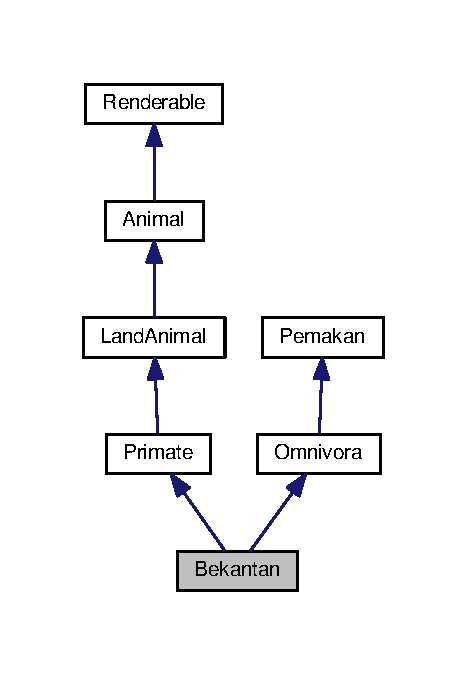
\includegraphics[width=224pt]{classBekantan__inherit__graph}
\end{center}
\end{figure}


Collaboration diagram for Bekantan\+:
\nopagebreak
\begin{figure}[H]
\begin{center}
\leavevmode
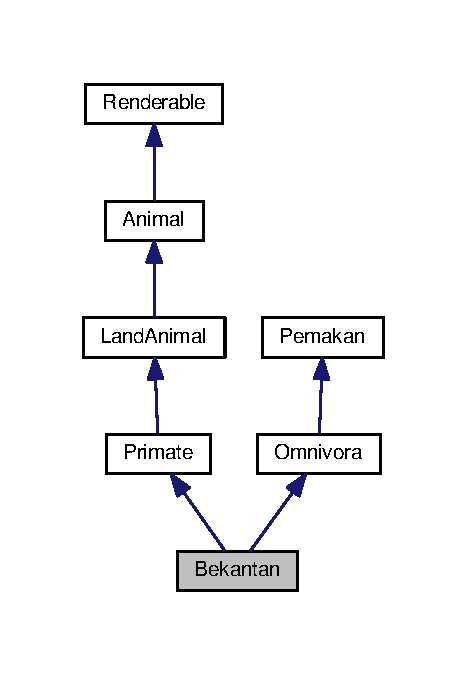
\includegraphics[width=224pt]{classBekantan__coll__graph}
\end{center}
\end{figure}
\subsection*{Public Member Functions}
\begin{DoxyCompactItemize}
\item 
\hyperlink{classBekantan_a00fa93f38b1aca4a25a989b495d45da1}{Bekantan} (int i, int x, int y, int massa, bool jinak)
\begin{DoxyCompactList}\small\item\em Constructor. Menciptakan \hyperlink{classBekantan}{Bekantan} dengan inisial \textquotesingle{}B\textquotesingle{} dan ID i. \end{DoxyCompactList}\item 
void \hyperlink{classBekantan_a1a21f2ea48a5c5ede8b988ce7a675468}{Interact} ()\hypertarget{classBekantan_a1a21f2ea48a5c5ede8b988ce7a675468}{}\label{classBekantan_a1a21f2ea48a5c5ede8b988ce7a675468}

\begin{DoxyCompactList}\small\item\em Menampilkan aksi binatang ke layar. \end{DoxyCompactList}\item 
int \hyperlink{classBekantan_a84c8ea3d97bd95d0c108d4016b5be934}{Get\+Jml\+Makanan} ()
\begin{DoxyCompactList}\small\item\em Melihat jumlah makanan dari binatang. Memanggil fungsi Get\+Amount parent \hyperlink{classOmnivora}{Omnivora}. \end{DoxyCompactList}\end{DoxyCompactItemize}
\subsection*{Additional Inherited Members}


\subsection{Detailed Description}
Kelas \hyperlink{classBekantan}{Bekantan} turunan dari kelas \hyperlink{classPrimate}{Primate} dan \hyperlink{classOmnivora}{Omnivora} 

\subsection{Constructor \& Destructor Documentation}
\index{Bekantan@{Bekantan}!Bekantan@{Bekantan}}
\index{Bekantan@{Bekantan}!Bekantan@{Bekantan}}
\subsubsection[{\texorpdfstring{Bekantan(int i, int x, int y, int massa, bool jinak)}{Bekantan(int i, int x, int y, int massa, bool jinak)}}]{\setlength{\rightskip}{0pt plus 5cm}Bekantan\+::\+Bekantan (
\begin{DoxyParamCaption}
\item[{int}]{i, }
\item[{int}]{x, }
\item[{int}]{y, }
\item[{int}]{massa, }
\item[{bool}]{jinak}
\end{DoxyParamCaption}
)}\hypertarget{classBekantan_a00fa93f38b1aca4a25a989b495d45da1}{}\label{classBekantan_a00fa93f38b1aca4a25a989b495d45da1}


Constructor. Menciptakan \hyperlink{classBekantan}{Bekantan} dengan inisial \textquotesingle{}B\textquotesingle{} dan ID i. 


\begin{DoxyParams}{Parameters}
{\em i} & Nilai Id \hyperlink{classAnimal}{Animal} yang diciptakan \\
\hline
{\em x} & Posisi x \hyperlink{classAnimal}{Animal} yang diciptakan \\
\hline
{\em y} & Posisi y \hyperlink{classAnimal}{Animal} yang diciptakan \\
\hline
{\em massa} & berat \hyperlink{classAnimal}{Animal} yang diciptakan \\
\hline
{\em jinak} & nilai jinak \hyperlink{classAnimal}{Animal} yang diciptakan \\
\hline
\end{DoxyParams}


\subsection{Member Function Documentation}
\index{Bekantan@{Bekantan}!Get\+Jml\+Makanan@{Get\+Jml\+Makanan}}
\index{Get\+Jml\+Makanan@{Get\+Jml\+Makanan}!Bekantan@{Bekantan}}
\subsubsection[{\texorpdfstring{Get\+Jml\+Makanan()}{GetJmlMakanan()}}]{\setlength{\rightskip}{0pt plus 5cm}int Bekantan\+::\+Get\+Jml\+Makanan (
\begin{DoxyParamCaption}
{}
\end{DoxyParamCaption}
)\hspace{0.3cm}{\ttfamily [virtual]}}\hypertarget{classBekantan_a84c8ea3d97bd95d0c108d4016b5be934}{}\label{classBekantan_a84c8ea3d97bd95d0c108d4016b5be934}


Melihat jumlah makanan dari binatang. Memanggil fungsi Get\+Amount parent \hyperlink{classOmnivora}{Omnivora}. 

\begin{DoxyReturn}{Returns}
Jumlah makanan dari binatang. 
\end{DoxyReturn}


Implements \hyperlink{classAnimal_a3f1cced7bac93f7c88a24ec5a0e989fe}{Animal}.



The documentation for this class was generated from the following files\+:\begin{DoxyCompactItemize}
\item 
listanimal.\+h\item 
listanimal.\+cpp\end{DoxyCompactItemize}

\hypertarget{classBuaya}{}\section{Buaya Class Reference}
\label{classBuaya}\index{Buaya@{Buaya}}


{\ttfamily \#include $<$listanimal.\+h$>$}



Inheritance diagram for Buaya\+:
\nopagebreak
\begin{figure}[H]
\begin{center}
\leavevmode
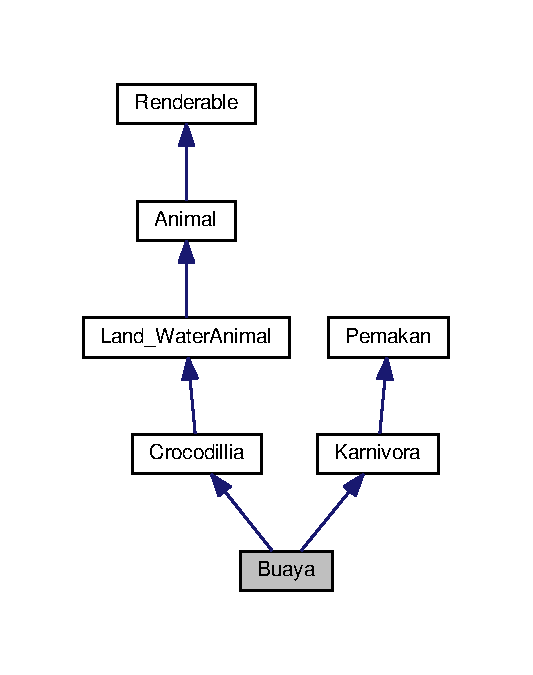
\includegraphics[width=256pt]{classBuaya__inherit__graph}
\end{center}
\end{figure}


Collaboration diagram for Buaya\+:
\nopagebreak
\begin{figure}[H]
\begin{center}
\leavevmode
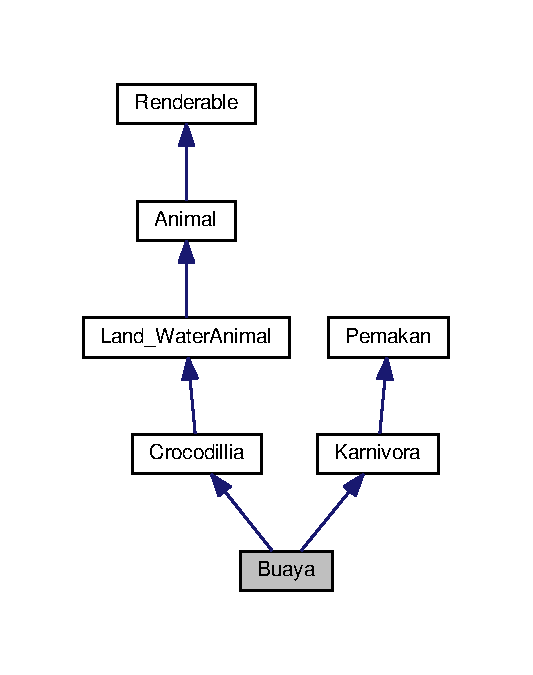
\includegraphics[width=256pt]{classBuaya__coll__graph}
\end{center}
\end{figure}
\subsection*{Public Member Functions}
\begin{DoxyCompactItemize}
\item 
\hyperlink{classBuaya_a56229331076a5f3cb5bf26a354b246d2}{Buaya} (int i, int x, int y, int massa, bool jinak)
\begin{DoxyCompactList}\small\item\em Constructor. Menciptakan \hyperlink{classBuaya}{Buaya} dengan inisial \textquotesingle{}D\textquotesingle{} dan ID i. \end{DoxyCompactList}\item 
void \hyperlink{classBuaya_a3ace61bd8605541c559b5922c2133869}{Interact} ()\hypertarget{classBuaya_a3ace61bd8605541c559b5922c2133869}{}\label{classBuaya_a3ace61bd8605541c559b5922c2133869}

\begin{DoxyCompactList}\small\item\em Menampilkan aksi binatang ke layar. \end{DoxyCompactList}\item 
int \hyperlink{classBuaya_a00f50933adea8ab884443d344f388bfb}{Get\+Jml\+Makanan} ()
\begin{DoxyCompactList}\small\item\em Melihat jumlah makanan dari binatang. Memanggil fungsi Get\+Amount parent \hyperlink{classKarnivora}{Karnivora}. \end{DoxyCompactList}\end{DoxyCompactItemize}
\subsection*{Additional Inherited Members}


\subsection{Detailed Description}
Kelas \hyperlink{classBuaya}{Buaya} turunan dari \hyperlink{classCrocodillia}{Crocodillia} dan \hyperlink{classKarnivora}{Karnivora} 

\subsection{Constructor \& Destructor Documentation}
\index{Buaya@{Buaya}!Buaya@{Buaya}}
\index{Buaya@{Buaya}!Buaya@{Buaya}}
\subsubsection[{\texorpdfstring{Buaya(int i, int x, int y, int massa, bool jinak)}{Buaya(int i, int x, int y, int massa, bool jinak)}}]{\setlength{\rightskip}{0pt plus 5cm}Buaya\+::\+Buaya (
\begin{DoxyParamCaption}
\item[{int}]{i, }
\item[{int}]{x, }
\item[{int}]{y, }
\item[{int}]{massa, }
\item[{bool}]{jinak}
\end{DoxyParamCaption}
)}\hypertarget{classBuaya_a56229331076a5f3cb5bf26a354b246d2}{}\label{classBuaya_a56229331076a5f3cb5bf26a354b246d2}


Constructor. Menciptakan \hyperlink{classBuaya}{Buaya} dengan inisial \textquotesingle{}D\textquotesingle{} dan ID i. 


\begin{DoxyParams}{Parameters}
{\em i} & Nilai Id \hyperlink{classAnimal}{Animal} yang diciptakan \\
\hline
{\em x} & Posisi x \hyperlink{classAnimal}{Animal} yang diciptakan \\
\hline
{\em y} & Posisi y \hyperlink{classAnimal}{Animal} yang diciptakan \\
\hline
{\em massa} & berat \hyperlink{classAnimal}{Animal} yang diciptakan \\
\hline
{\em jinak} & nilai jinak \hyperlink{classAnimal}{Animal} yang diciptakan \\
\hline
\end{DoxyParams}


\subsection{Member Function Documentation}
\index{Buaya@{Buaya}!Get\+Jml\+Makanan@{Get\+Jml\+Makanan}}
\index{Get\+Jml\+Makanan@{Get\+Jml\+Makanan}!Buaya@{Buaya}}
\subsubsection[{\texorpdfstring{Get\+Jml\+Makanan()}{GetJmlMakanan()}}]{\setlength{\rightskip}{0pt plus 5cm}int Buaya\+::\+Get\+Jml\+Makanan (
\begin{DoxyParamCaption}
{}
\end{DoxyParamCaption}
)\hspace{0.3cm}{\ttfamily [virtual]}}\hypertarget{classBuaya_a00f50933adea8ab884443d344f388bfb}{}\label{classBuaya_a00f50933adea8ab884443d344f388bfb}


Melihat jumlah makanan dari binatang. Memanggil fungsi Get\+Amount parent \hyperlink{classKarnivora}{Karnivora}. 

\begin{DoxyReturn}{Returns}
Jumlah makanan dari binatang. 
\end{DoxyReturn}


Implements \hyperlink{classAnimal_a3f1cced7bac93f7c88a24ec5a0e989fe}{Animal}.



The documentation for this class was generated from the following files\+:\begin{DoxyCompactItemize}
\item 
listanimal.\+h\item 
listanimal.\+cpp\end{DoxyCompactItemize}

\hypertarget{classCage}{}\section{Cage Class Reference}
\label{classCage}\index{Cage@{Cage}}


{\ttfamily \#include $<$cage.\+h$>$}

\subsection*{Public Member Functions}
\begin{DoxyCompactItemize}
\item 
\hyperlink{classCage_ad281dd303f3e6f810a89d51af1c91443}{Cage} (int \+\_\+id, char hab)
\begin{DoxyCompactList}\small\item\em Constructor. Menciptakan \hyperlink{classCage}{Cage} dengan id \+\_\+id dan habitat hab. \end{DoxyCompactList}\item 
void \hyperlink{classCage_ad9f2bbc36b168b9a1eed1f575206e37a}{Add\+Animal} (\hyperlink{classAnimal}{Animal} $\ast$a)
\begin{DoxyCompactList}\small\item\em Menambahkan elemen ke animal. \end{DoxyCompactList}\item 
void \hyperlink{classCage_a814423376e6a50f31d33fea857fef9d5}{Add\+Cell} (char c)
\begin{DoxyCompactList}\small\item\em Menambahkan cell Penambahan cell akan menambah luas dari cage. \end{DoxyCompactList}\item 
int \hyperlink{classCage_a105581dec308e734a7527d420d7cb4ee}{Get\+Id} ()
\begin{DoxyCompactList}\small\item\em Getter id. \end{DoxyCompactList}\item 
int \hyperlink{classCage_a10136c36884c5c58f6c244afbeee120f}{Get\+Luas} ()
\begin{DoxyCompactList}\small\item\em Getter luas. \end{DoxyCompactList}\item 
int \hyperlink{classCage_a7d94436b894f2e5496ee467743bd2bcc}{Get\+Nb\+Animal} ()
\begin{DoxyCompactList}\small\item\em Mengembalikan banyaknya elemen animal. \end{DoxyCompactList}\item 
char \hyperlink{classCage_a745590ba0bb6f530762d7a64884d5ec6}{Get\+Habitat} ()
\begin{DoxyCompactList}\small\item\em Getter habitat. \end{DoxyCompactList}\item 
bool \hyperlink{classCage_a731496cc568257acdb67fa967dfca577}{Is\+Available} ()
\begin{DoxyCompactList}\small\item\em Mengetahui apakah cage available Mengecek apakah cage dapat ditambahkan elemen animal. \end{DoxyCompactList}\item 
bool \hyperlink{classCage_a5d34dbb0a9acc972234f639e5ea9e8ea}{Is\+Isi\+Jinak} ()
\begin{DoxyCompactList}\small\item\em Mengetahui apakah elemen animal jinak. \end{DoxyCompactList}\end{DoxyCompactItemize}


\subsection{Detailed Description}
Kelas \hyperlink{classCage}{Cage} terdiri dari animal dengan luas, id, dan habitat tertentu Representasi kumpulan cage dengan habitat sejenis 

\subsection{Constructor \& Destructor Documentation}
\index{Cage@{Cage}!Cage@{Cage}}
\index{Cage@{Cage}!Cage@{Cage}}
\subsubsection[{\texorpdfstring{Cage(int \+\_\+id, char hab)}{Cage(int _id, char hab)}}]{\setlength{\rightskip}{0pt plus 5cm}Cage\+::\+Cage (
\begin{DoxyParamCaption}
\item[{int}]{\+\_\+id, }
\item[{char}]{hab}
\end{DoxyParamCaption}
)}\hypertarget{classCage_ad281dd303f3e6f810a89d51af1c91443}{}\label{classCage_ad281dd303f3e6f810a89d51af1c91443}


Constructor. Menciptakan \hyperlink{classCage}{Cage} dengan id \+\_\+id dan habitat hab. 


\begin{DoxyParams}{Parameters}
{\em \+\_\+id} & Nilai id \hyperlink{classCage}{Cage} yang ingin diciptakan \\
\hline
{\em hab} & Nilai habitat \hyperlink{classCage}{Cage} yang ingin diciptakan \\
\hline
\end{DoxyParams}


\subsection{Member Function Documentation}
\index{Cage@{Cage}!Add\+Animal@{Add\+Animal}}
\index{Add\+Animal@{Add\+Animal}!Cage@{Cage}}
\subsubsection[{\texorpdfstring{Add\+Animal(\+Animal $\ast$a)}{AddAnimal(Animal *a)}}]{\setlength{\rightskip}{0pt plus 5cm}void Cage\+::\+Add\+Animal (
\begin{DoxyParamCaption}
\item[{{\bf Animal} $\ast$}]{a}
\end{DoxyParamCaption}
)}\hypertarget{classCage_ad9f2bbc36b168b9a1eed1f575206e37a}{}\label{classCage_ad9f2bbc36b168b9a1eed1f575206e37a}


Menambahkan elemen ke animal. 


\begin{DoxyParams}{Parameters}
{\em a} & elemen yang ingin ditambahkan ke animal \\
\hline
\end{DoxyParams}
\index{Cage@{Cage}!Add\+Cell@{Add\+Cell}}
\index{Add\+Cell@{Add\+Cell}!Cage@{Cage}}
\subsubsection[{\texorpdfstring{Add\+Cell(char c)}{AddCell(char c)}}]{\setlength{\rightskip}{0pt plus 5cm}void Cage\+::\+Add\+Cell (
\begin{DoxyParamCaption}
\item[{char}]{c}
\end{DoxyParamCaption}
)}\hypertarget{classCage_a814423376e6a50f31d33fea857fef9d5}{}\label{classCage_a814423376e6a50f31d33fea857fef9d5}


Menambahkan cell Penambahan cell akan menambah luas dari cage. 


\begin{DoxyParams}{Parameters}
{\em c} & \hyperlink{classHabitat}{Habitat} \\
\hline
\end{DoxyParams}
\index{Cage@{Cage}!Get\+Habitat@{Get\+Habitat}}
\index{Get\+Habitat@{Get\+Habitat}!Cage@{Cage}}
\subsubsection[{\texorpdfstring{Get\+Habitat()}{GetHabitat()}}]{\setlength{\rightskip}{0pt plus 5cm}char Cage\+::\+Get\+Habitat (
\begin{DoxyParamCaption}
{}
\end{DoxyParamCaption}
)}\hypertarget{classCage_a745590ba0bb6f530762d7a64884d5ec6}{}\label{classCage_a745590ba0bb6f530762d7a64884d5ec6}


Getter habitat. 

\begin{DoxyReturn}{Returns}
habitat 
\end{DoxyReturn}
\index{Cage@{Cage}!Get\+Id@{Get\+Id}}
\index{Get\+Id@{Get\+Id}!Cage@{Cage}}
\subsubsection[{\texorpdfstring{Get\+Id()}{GetId()}}]{\setlength{\rightskip}{0pt plus 5cm}int Cage\+::\+Get\+Id (
\begin{DoxyParamCaption}
{}
\end{DoxyParamCaption}
)}\hypertarget{classCage_a105581dec308e734a7527d420d7cb4ee}{}\label{classCage_a105581dec308e734a7527d420d7cb4ee}


Getter id. 

\begin{DoxyReturn}{Returns}
id 
\end{DoxyReturn}
\index{Cage@{Cage}!Get\+Luas@{Get\+Luas}}
\index{Get\+Luas@{Get\+Luas}!Cage@{Cage}}
\subsubsection[{\texorpdfstring{Get\+Luas()}{GetLuas()}}]{\setlength{\rightskip}{0pt plus 5cm}int Cage\+::\+Get\+Luas (
\begin{DoxyParamCaption}
{}
\end{DoxyParamCaption}
)}\hypertarget{classCage_a10136c36884c5c58f6c244afbeee120f}{}\label{classCage_a10136c36884c5c58f6c244afbeee120f}


Getter luas. 

\begin{DoxyReturn}{Returns}
luas 
\end{DoxyReturn}
\index{Cage@{Cage}!Get\+Nb\+Animal@{Get\+Nb\+Animal}}
\index{Get\+Nb\+Animal@{Get\+Nb\+Animal}!Cage@{Cage}}
\subsubsection[{\texorpdfstring{Get\+Nb\+Animal()}{GetNbAnimal()}}]{\setlength{\rightskip}{0pt plus 5cm}int Cage\+::\+Get\+Nb\+Animal (
\begin{DoxyParamCaption}
{}
\end{DoxyParamCaption}
)}\hypertarget{classCage_a7d94436b894f2e5496ee467743bd2bcc}{}\label{classCage_a7d94436b894f2e5496ee467743bd2bcc}


Mengembalikan banyaknya elemen animal. 

\begin{DoxyReturn}{Returns}
size dari animal 
\end{DoxyReturn}
\index{Cage@{Cage}!Is\+Available@{Is\+Available}}
\index{Is\+Available@{Is\+Available}!Cage@{Cage}}
\subsubsection[{\texorpdfstring{Is\+Available()}{IsAvailable()}}]{\setlength{\rightskip}{0pt plus 5cm}bool Cage\+::\+Is\+Available (
\begin{DoxyParamCaption}
{}
\end{DoxyParamCaption}
)}\hypertarget{classCage_a731496cc568257acdb67fa967dfca577}{}\label{classCage_a731496cc568257acdb67fa967dfca577}


Mengetahui apakah cage available Mengecek apakah cage dapat ditambahkan elemen animal. 

\begin{DoxyReturn}{Returns}
Apakah cage availabe 
\end{DoxyReturn}
\index{Cage@{Cage}!Is\+Isi\+Jinak@{Is\+Isi\+Jinak}}
\index{Is\+Isi\+Jinak@{Is\+Isi\+Jinak}!Cage@{Cage}}
\subsubsection[{\texorpdfstring{Is\+Isi\+Jinak()}{IsIsiJinak()}}]{\setlength{\rightskip}{0pt plus 5cm}bool Cage\+::\+Is\+Isi\+Jinak (
\begin{DoxyParamCaption}
{}
\end{DoxyParamCaption}
)}\hypertarget{classCage_a5d34dbb0a9acc972234f639e5ea9e8ea}{}\label{classCage_a5d34dbb0a9acc972234f639e5ea9e8ea}


Mengetahui apakah elemen animal jinak. 

\begin{DoxyReturn}{Returns}
Apakah semua elemen animal jinak 
\end{DoxyReturn}


The documentation for this class was generated from the following files\+:\begin{DoxyCompactItemize}
\item 
cage.\+h\item 
cage.\+cpp\end{DoxyCompactItemize}

\hypertarget{classCageHandler}{}\section{Cage\+Handler Class Reference}
\label{classCageHandler}\index{Cage\+Handler@{Cage\+Handler}}


{\ttfamily \#include $<$cage.\+h$>$}

\subsection*{Public Member Functions}
\begin{DoxyCompactItemize}
\item 
\hyperlink{classCageHandler_a7f611d145a35ec9037196beb280f0d15}{Cage\+Handler} ()\hypertarget{classCageHandler_a7f611d145a35ec9037196beb280f0d15}{}\label{classCageHandler_a7f611d145a35ec9037196beb280f0d15}

\begin{DoxyCompactList}\small\item\em Constructor Menciptakan \hyperlink{classCageHandler}{Cage\+Handler} dengan n=0. \end{DoxyCompactList}\item 
\hyperlink{classCageHandler_aeb3227fcc447d3dbb36636335f7f0235}{$\sim$\+Cage\+Handler} ()\hypertarget{classCageHandler_aeb3227fcc447d3dbb36636335f7f0235}{}\label{classCageHandler_aeb3227fcc447d3dbb36636335f7f0235}

\begin{DoxyCompactList}\small\item\em Destructor. \end{DoxyCompactList}\item 
\hyperlink{classCage}{Cage} $\ast$ \hyperlink{classCageHandler_a8564d2b8d6326c1f6771143b82951a64}{Get\+Cage} (int id)
\begin{DoxyCompactList}\small\item\em Getter elemen list\+\_\+cage. \end{DoxyCompactList}\item 
int \hyperlink{classCageHandler_aaf499991ae721d645daa9e655efc5b5d}{Nb\+Cage} ()
\begin{DoxyCompactList}\small\item\em Mengetahui banyak cage yang diciptakan. \end{DoxyCompactList}\item 
void \hyperlink{classCageHandler_a83693282e69e750f89a0973b042a4297}{Add\+Cage} (\hyperlink{classCage}{Cage} $\ast$c)
\begin{DoxyCompactList}\small\item\em Menambahkan cage kedalam list\+\_\+cage. \end{DoxyCompactList}\end{DoxyCompactItemize}


\subsection{Detailed Description}
Kelas \hyperlink{classCageHandler}{Cage\+Handler} terdiri dari semua cage yang pernah diciptakan 

\subsection{Member Function Documentation}
\index{Cage\+Handler@{Cage\+Handler}!Add\+Cage@{Add\+Cage}}
\index{Add\+Cage@{Add\+Cage}!Cage\+Handler@{Cage\+Handler}}
\subsubsection[{\texorpdfstring{Add\+Cage(\+Cage $\ast$c)}{AddCage(Cage *c)}}]{\setlength{\rightskip}{0pt plus 5cm}void Cage\+Handler\+::\+Add\+Cage (
\begin{DoxyParamCaption}
\item[{{\bf Cage} $\ast$}]{c}
\end{DoxyParamCaption}
)}\hypertarget{classCageHandler_a83693282e69e750f89a0973b042a4297}{}\label{classCageHandler_a83693282e69e750f89a0973b042a4297}


Menambahkan cage kedalam list\+\_\+cage. 


\begin{DoxyParams}{Parameters}
{\em c} & elemen yang ingin ditambahkan ke list\+\_\+cage \\
\hline
\end{DoxyParams}
\index{Cage\+Handler@{Cage\+Handler}!Get\+Cage@{Get\+Cage}}
\index{Get\+Cage@{Get\+Cage}!Cage\+Handler@{Cage\+Handler}}
\subsubsection[{\texorpdfstring{Get\+Cage(int id)}{GetCage(int id)}}]{\setlength{\rightskip}{0pt plus 5cm}{\bf Cage} $\ast$ Cage\+Handler\+::\+Get\+Cage (
\begin{DoxyParamCaption}
\item[{int}]{id}
\end{DoxyParamCaption}
)}\hypertarget{classCageHandler_a8564d2b8d6326c1f6771143b82951a64}{}\label{classCageHandler_a8564d2b8d6326c1f6771143b82951a64}


Getter elemen list\+\_\+cage. 


\begin{DoxyParams}{Parameters}
{\em id} & Nilai posisi elemen yang ingin didapatkan \\
\hline
\end{DoxyParams}
\begin{DoxyReturn}{Returns}
list\+\_\+cage\mbox{[}id\mbox{]} 
\end{DoxyReturn}
\index{Cage\+Handler@{Cage\+Handler}!Nb\+Cage@{Nb\+Cage}}
\index{Nb\+Cage@{Nb\+Cage}!Cage\+Handler@{Cage\+Handler}}
\subsubsection[{\texorpdfstring{Nb\+Cage()}{NbCage()}}]{\setlength{\rightskip}{0pt plus 5cm}int Cage\+Handler\+::\+Nb\+Cage (
\begin{DoxyParamCaption}
{}
\end{DoxyParamCaption}
)}\hypertarget{classCageHandler_aaf499991ae721d645daa9e655efc5b5d}{}\label{classCageHandler_aaf499991ae721d645daa9e655efc5b5d}


Mengetahui banyak cage yang diciptakan. 

\begin{DoxyReturn}{Returns}
n 
\end{DoxyReturn}


The documentation for this class was generated from the following files\+:\begin{DoxyCompactItemize}
\item 
cage.\+h\item 
cage.\+cpp\end{DoxyCompactItemize}

\hypertarget{classCarchanhiniformes}{}\section{Carchanhiniformes Class Reference}
\label{classCarchanhiniformes}\index{Carchanhiniformes@{Carchanhiniformes}}


{\ttfamily \#include $<$animal.\+h$>$}



\subsection{Detailed Description}
Kelas \hyperlink{classCarchanhiniformes}{Carchanhiniformes} turunan dari \hyperlink{classWaterAnimal}{Water\+Animal} menunjukkan ordo hiu 

The documentation for this class was generated from the following file\+:\begin{DoxyCompactItemize}
\item 
animal.\+h\end{DoxyCompactItemize}

\hypertarget{classCarcharhiniformes}{}\section{Carcharhiniformes Class Reference}
\label{classCarcharhiniformes}\index{Carcharhiniformes@{Carcharhiniformes}}


Inheritance diagram for Carcharhiniformes\+:
\nopagebreak
\begin{figure}[H]
\begin{center}
\leavevmode
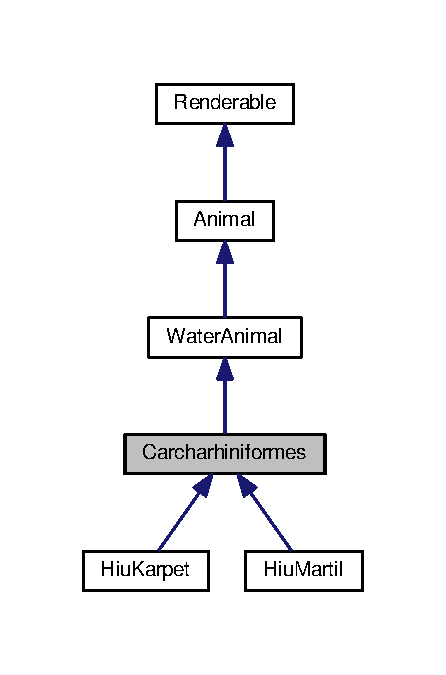
\includegraphics[width=214pt]{classCarcharhiniformes__inherit__graph}
\end{center}
\end{figure}


Collaboration diagram for Carcharhiniformes\+:
\nopagebreak
\begin{figure}[H]
\begin{center}
\leavevmode
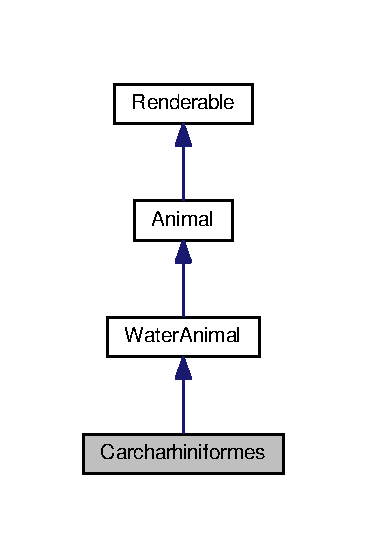
\includegraphics[width=176pt]{classCarcharhiniformes__coll__graph}
\end{center}
\end{figure}
\subsection*{Public Member Functions}
\begin{DoxyCompactItemize}
\item 
\hyperlink{classCarcharhiniformes_af9d3c39c3fcafd49ea7cea9212ac08e3}{Carcharhiniformes} (char c, int i)
\begin{DoxyCompactList}\small\item\em Constructor. Menciptakan \hyperlink{classCarcharhiniformes}{Carcharhiniformes} dengan memanggil constructor \hyperlink{classWaterAnimal}{Water\+Animal} berinisial c dan ID i. \end{DoxyCompactList}\end{DoxyCompactItemize}
\subsection*{Additional Inherited Members}


\subsection{Constructor \& Destructor Documentation}
\index{Carcharhiniformes@{Carcharhiniformes}!Carcharhiniformes@{Carcharhiniformes}}
\index{Carcharhiniformes@{Carcharhiniformes}!Carcharhiniformes@{Carcharhiniformes}}
\subsubsection[{\texorpdfstring{Carcharhiniformes(char c, int i)}{Carcharhiniformes(char c, int i)}}]{\setlength{\rightskip}{0pt plus 5cm}Carcharhiniformes\+::\+Carcharhiniformes (
\begin{DoxyParamCaption}
\item[{char}]{c, }
\item[{int}]{i}
\end{DoxyParamCaption}
)}\hypertarget{classCarcharhiniformes_af9d3c39c3fcafd49ea7cea9212ac08e3}{}\label{classCarcharhiniformes_af9d3c39c3fcafd49ea7cea9212ac08e3}


Constructor. Menciptakan \hyperlink{classCarcharhiniformes}{Carcharhiniformes} dengan memanggil constructor \hyperlink{classWaterAnimal}{Water\+Animal} berinisial c dan ID i. 


\begin{DoxyParams}{Parameters}
{\em c} & inisial \hyperlink{classCarcharhiniformes}{Carcharhiniformes} yang ingin diciptakan \\
\hline
{\em i} & ID \hyperlink{classCarcharhiniformes}{Carcharhiniformes} yang ingin diciptakan \\
\hline
\end{DoxyParams}


The documentation for this class was generated from the following files\+:\begin{DoxyCompactItemize}
\item 
animal.\+h\item 
animal.\+cpp\end{DoxyCompactItemize}

\hypertarget{classCarnivore}{}\section{Carnivore Class Reference}
\label{classCarnivore}\index{Carnivore@{Carnivore}}


{\ttfamily \#include $<$animal.\+h$>$}



Inheritance diagram for Carnivore\+:
\nopagebreak
\begin{figure}[H]
\begin{center}
\leavevmode
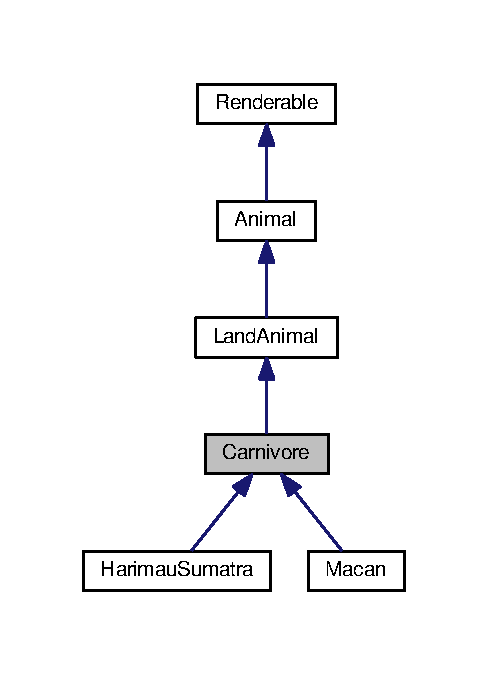
\includegraphics[width=234pt]{classCarnivore__inherit__graph}
\end{center}
\end{figure}


Collaboration diagram for Carnivore\+:
\nopagebreak
\begin{figure}[H]
\begin{center}
\leavevmode
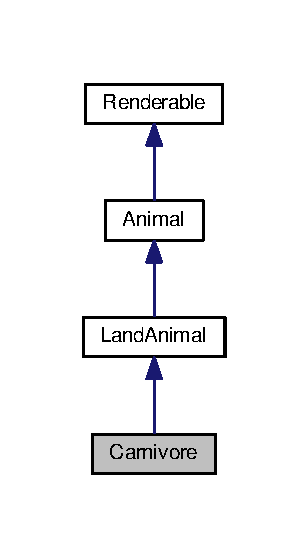
\includegraphics[width=148pt]{classCarnivore__coll__graph}
\end{center}
\end{figure}
\subsection*{Public Member Functions}
\begin{DoxyCompactItemize}
\item 
\hyperlink{classCarnivore_ad31797dd174b12c93a12925a6660196f}{Carnivore} (char c, int i)
\begin{DoxyCompactList}\small\item\em Constructor. Menciptakan \hyperlink{classCarnivore}{Carnivore} dengan memanggil constructor \hyperlink{classLandAnimal}{Land\+Animal} berinisial c dan ID i. \end{DoxyCompactList}\end{DoxyCompactItemize}
\subsection*{Additional Inherited Members}


\subsection{Detailed Description}
Kelas \hyperlink{classCarnivore}{Carnivore} turunan dari \hyperlink{classLandAnimal}{Land\+Animal} menunjukkan ordo karnivora 

\subsection{Constructor \& Destructor Documentation}
\index{Carnivore@{Carnivore}!Carnivore@{Carnivore}}
\index{Carnivore@{Carnivore}!Carnivore@{Carnivore}}
\subsubsection[{\texorpdfstring{Carnivore(char c, int i)}{Carnivore(char c, int i)}}]{\setlength{\rightskip}{0pt plus 5cm}Carnivore\+::\+Carnivore (
\begin{DoxyParamCaption}
\item[{char}]{c, }
\item[{int}]{i}
\end{DoxyParamCaption}
)}\hypertarget{classCarnivore_ad31797dd174b12c93a12925a6660196f}{}\label{classCarnivore_ad31797dd174b12c93a12925a6660196f}


Constructor. Menciptakan \hyperlink{classCarnivore}{Carnivore} dengan memanggil constructor \hyperlink{classLandAnimal}{Land\+Animal} berinisial c dan ID i. 


\begin{DoxyParams}{Parameters}
{\em c} & inisial \hyperlink{classCarnivore}{Carnivore} yang ingin diciptakan \\
\hline
{\em i} & ID \hyperlink{classCarnivore}{Carnivore} yang ingin diciptakan \\
\hline
\end{DoxyParams}


The documentation for this class was generated from the following files\+:\begin{DoxyCompactItemize}
\item 
animal.\+h\item 
animal.\+cpp\end{DoxyCompactItemize}

\hypertarget{classCell}{}\section{Cell Class Reference}
\label{classCell}\index{Cell@{Cell}}


{\ttfamily \#include $<$zoo.\+h$>$}



Inheritance diagram for Cell\+:
\nopagebreak
\begin{figure}[H]
\begin{center}
\leavevmode
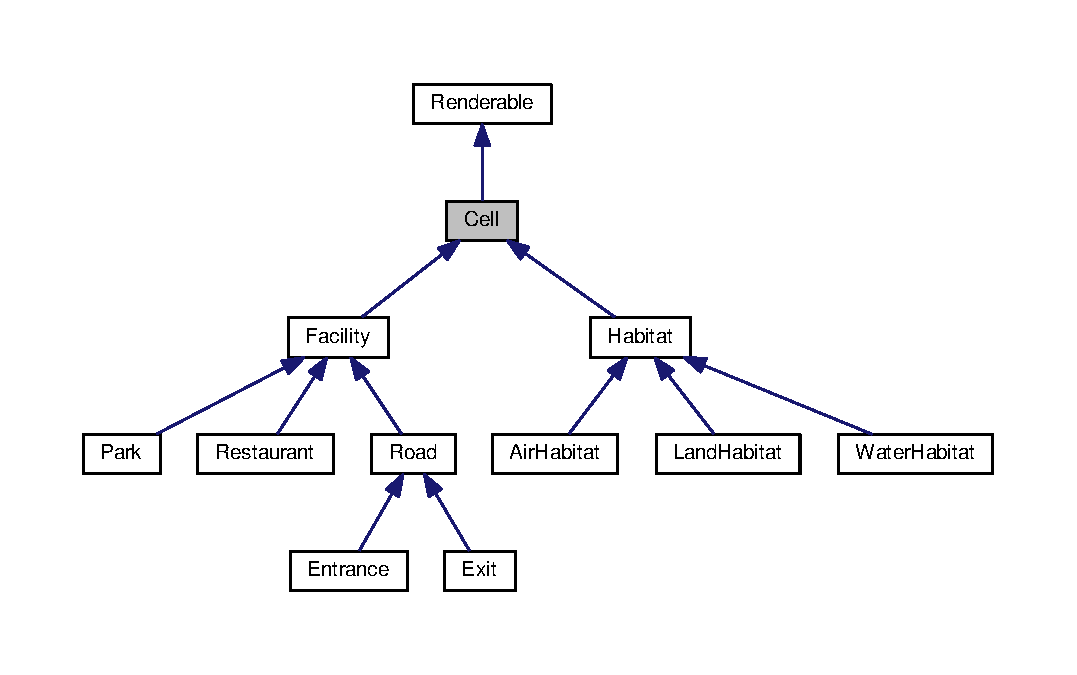
\includegraphics[width=350pt]{classCell__inherit__graph}
\end{center}
\end{figure}


Collaboration diagram for Cell\+:
\nopagebreak
\begin{figure}[H]
\begin{center}
\leavevmode
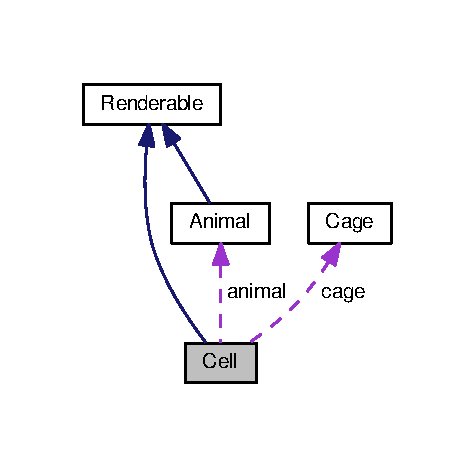
\includegraphics[width=228pt]{classCell__coll__graph}
\end{center}
\end{figure}
\subsection*{Public Member Functions}
\begin{DoxyCompactItemize}
\item 
\hyperlink{classCell_a7025ace286306aa5b6e09ccf43ac3451}{Cell} (char c, int x, int y)
\begin{DoxyCompactList}\small\item\em Constructor. Menciptakan \hyperlink{classCell}{Cell} kosong dengan type c, posisi $<$x,y$>$. \end{DoxyCompactList}\item 
virtual void \hyperlink{classCell_a6abd6c362b1b97636dd55ba46609c873}{Render} ()\hypertarget{classCell_a6abd6c362b1b97636dd55ba46609c873}{}\label{classCell_a6abd6c362b1b97636dd55ba46609c873}

\begin{DoxyCompactList}\small\item\em Menampilkan type cell Menuliskan type dari cell ke layar. \end{DoxyCompactList}\item 
char \hyperlink{classCell_abd27056583a21ced96605cab3495481d}{Get\+Type} ()
\begin{DoxyCompactList}\small\item\em Getter type. \end{DoxyCompactList}\item 
\hyperlink{classCage}{Cage} $\ast$ \hyperlink{classCell_a690c7e26b983879381406a0cf5a815a1}{Get\+Cage} ()
\begin{DoxyCompactList}\small\item\em Getter cage. \end{DoxyCompactList}\item 
void \hyperlink{classCell_ae7b402402a5fbd71db91eeed6e2697c8}{Set\+Cage} (\hyperlink{classCage}{Cage} $\ast$c)
\begin{DoxyCompactList}\small\item\em Setter cage. Merubah nilai cage dari cell. \end{DoxyCompactList}\item 
\hyperlink{classAnimal}{Animal} $\ast$ \hyperlink{classCell_aef420cdd18435ea7a2c8d96720fe8e7a}{Get\+Animal} ()
\begin{DoxyCompactList}\small\item\em Getter \hyperlink{classAnimal}{Animal}. \end{DoxyCompactList}\item 
void \hyperlink{classCell_a20c2142de099ddb1f6fa794aa3f5f26d}{Set\+Animal} (\hyperlink{classAnimal}{Animal} $\ast$a)
\begin{DoxyCompactList}\small\item\em Setter animal. Merubah nilai animal dari cell. \end{DoxyCompactList}\item 
int \hyperlink{classCell_a2026adcc21f0b3f6e38e8c50684e641c}{Get\+Absis} ()
\begin{DoxyCompactList}\small\item\em Getter absis. \end{DoxyCompactList}\item 
int \hyperlink{classCell_a5c243fe5ec6b7d879dee6560a72dadf5}{Get\+Ordinat} ()
\begin{DoxyCompactList}\small\item\em Getter absis. \end{DoxyCompactList}\end{DoxyCompactItemize}
\subsection*{Protected Attributes}
\begin{DoxyCompactItemize}
\item 
\hyperlink{classCage}{Cage} $\ast$ {\bfseries cage}\hypertarget{classCell_aec7f7f73c84c0300c0f6773780b32caa}{}\label{classCell_aec7f7f73c84c0300c0f6773780b32caa}

\item 
\hyperlink{classAnimal}{Animal} $\ast$ {\bfseries animal}\hypertarget{classCell_a98c459e9033110cdb8e2f37e0a936d82}{}\label{classCell_a98c459e9033110cdb8e2f37e0a936d82}

\item 
const char {\bfseries type}\hypertarget{classCell_a1968596db353a334cf526f9e4fae3c73}{}\label{classCell_a1968596db353a334cf526f9e4fae3c73}

\item 
const int {\bfseries absis}\hypertarget{classCell_a8133fdd0215fa37484eef356b527f04e}{}\label{classCell_a8133fdd0215fa37484eef356b527f04e}

\item 
const int {\bfseries ordinat}\hypertarget{classCell_a4215afbb62efea409933703ca8e95db6}{}\label{classCell_a4215afbb62efea409933703ca8e95db6}

\end{DoxyCompactItemize}
\subsection*{Additional Inherited Members}


\subsection{Detailed Description}
Kelas \hyperlink{classCell}{Cell} menyimpan informasi cage dan animal inherit kelas \hyperlink{classRenderable}{Renderable} 

\subsection{Constructor \& Destructor Documentation}
\index{Cell@{Cell}!Cell@{Cell}}
\index{Cell@{Cell}!Cell@{Cell}}
\subsubsection[{\texorpdfstring{Cell(char c, int x, int y)}{Cell(char c, int x, int y)}}]{\setlength{\rightskip}{0pt plus 5cm}Cell\+::\+Cell (
\begin{DoxyParamCaption}
\item[{char}]{c, }
\item[{int}]{x, }
\item[{int}]{y}
\end{DoxyParamCaption}
)}\hypertarget{classCell_a7025ace286306aa5b6e09ccf43ac3451}{}\label{classCell_a7025ace286306aa5b6e09ccf43ac3451}


Constructor. Menciptakan \hyperlink{classCell}{Cell} kosong dengan type c, posisi $<$x,y$>$. 


\begin{DoxyParams}{Parameters}
{\em c} & Nilai type \hyperlink{classCell}{Cell} yang ingin dibuat \\
\hline
{\em x} & Nilai absis \hyperlink{classCell}{Cell} yang ingin dibuat \\
\hline
{\em y} & Nilai ordinat \hyperlink{classCell}{Cell} yang ingin dibuat \\
\hline
\end{DoxyParams}


\subsection{Member Function Documentation}
\index{Cell@{Cell}!Get\+Absis@{Get\+Absis}}
\index{Get\+Absis@{Get\+Absis}!Cell@{Cell}}
\subsubsection[{\texorpdfstring{Get\+Absis()}{GetAbsis()}}]{\setlength{\rightskip}{0pt plus 5cm}int Cell\+::\+Get\+Absis (
\begin{DoxyParamCaption}
{}
\end{DoxyParamCaption}
)}\hypertarget{classCell_a2026adcc21f0b3f6e38e8c50684e641c}{}\label{classCell_a2026adcc21f0b3f6e38e8c50684e641c}


Getter absis. 

\begin{DoxyReturn}{Returns}
absis 
\end{DoxyReturn}
\index{Cell@{Cell}!Get\+Animal@{Get\+Animal}}
\index{Get\+Animal@{Get\+Animal}!Cell@{Cell}}
\subsubsection[{\texorpdfstring{Get\+Animal()}{GetAnimal()}}]{\setlength{\rightskip}{0pt plus 5cm}{\bf Animal} $\ast$ Cell\+::\+Get\+Animal (
\begin{DoxyParamCaption}
{}
\end{DoxyParamCaption}
)}\hypertarget{classCell_aef420cdd18435ea7a2c8d96720fe8e7a}{}\label{classCell_aef420cdd18435ea7a2c8d96720fe8e7a}


Getter \hyperlink{classAnimal}{Animal}. 

\begin{DoxyReturn}{Returns}
animal 
\end{DoxyReturn}
\index{Cell@{Cell}!Get\+Cage@{Get\+Cage}}
\index{Get\+Cage@{Get\+Cage}!Cell@{Cell}}
\subsubsection[{\texorpdfstring{Get\+Cage()}{GetCage()}}]{\setlength{\rightskip}{0pt plus 5cm}{\bf Cage} $\ast$ Cell\+::\+Get\+Cage (
\begin{DoxyParamCaption}
{}
\end{DoxyParamCaption}
)}\hypertarget{classCell_a690c7e26b983879381406a0cf5a815a1}{}\label{classCell_a690c7e26b983879381406a0cf5a815a1}


Getter cage. 

\begin{DoxyReturn}{Returns}
cage 
\end{DoxyReturn}
\index{Cell@{Cell}!Get\+Ordinat@{Get\+Ordinat}}
\index{Get\+Ordinat@{Get\+Ordinat}!Cell@{Cell}}
\subsubsection[{\texorpdfstring{Get\+Ordinat()}{GetOrdinat()}}]{\setlength{\rightskip}{0pt plus 5cm}int Cell\+::\+Get\+Ordinat (
\begin{DoxyParamCaption}
{}
\end{DoxyParamCaption}
)}\hypertarget{classCell_a5c243fe5ec6b7d879dee6560a72dadf5}{}\label{classCell_a5c243fe5ec6b7d879dee6560a72dadf5}


Getter absis. 

\begin{DoxyReturn}{Returns}
absis 
\end{DoxyReturn}
\index{Cell@{Cell}!Get\+Type@{Get\+Type}}
\index{Get\+Type@{Get\+Type}!Cell@{Cell}}
\subsubsection[{\texorpdfstring{Get\+Type()}{GetType()}}]{\setlength{\rightskip}{0pt plus 5cm}char Cell\+::\+Get\+Type (
\begin{DoxyParamCaption}
{}
\end{DoxyParamCaption}
)}\hypertarget{classCell_abd27056583a21ced96605cab3495481d}{}\label{classCell_abd27056583a21ced96605cab3495481d}


Getter type. 

\begin{DoxyReturn}{Returns}
type 
\end{DoxyReturn}
\index{Cell@{Cell}!Set\+Animal@{Set\+Animal}}
\index{Set\+Animal@{Set\+Animal}!Cell@{Cell}}
\subsubsection[{\texorpdfstring{Set\+Animal(\+Animal $\ast$a)}{SetAnimal(Animal *a)}}]{\setlength{\rightskip}{0pt plus 5cm}void Cell\+::\+Set\+Animal (
\begin{DoxyParamCaption}
\item[{{\bf Animal} $\ast$}]{a}
\end{DoxyParamCaption}
)}\hypertarget{classCell_a20c2142de099ddb1f6fa794aa3f5f26d}{}\label{classCell_a20c2142de099ddb1f6fa794aa3f5f26d}


Setter animal. Merubah nilai animal dari cell. 


\begin{DoxyParams}{Parameters}
{\em a} & Nilai animal yang ingin dimasukkan kedalam cell \\
\hline
\end{DoxyParams}
\index{Cell@{Cell}!Set\+Cage@{Set\+Cage}}
\index{Set\+Cage@{Set\+Cage}!Cell@{Cell}}
\subsubsection[{\texorpdfstring{Set\+Cage(\+Cage $\ast$c)}{SetCage(Cage *c)}}]{\setlength{\rightskip}{0pt plus 5cm}void Cell\+::\+Set\+Cage (
\begin{DoxyParamCaption}
\item[{{\bf Cage} $\ast$}]{c}
\end{DoxyParamCaption}
)}\hypertarget{classCell_ae7b402402a5fbd71db91eeed6e2697c8}{}\label{classCell_ae7b402402a5fbd71db91eeed6e2697c8}


Setter cage. Merubah nilai cage dari cell. 


\begin{DoxyParams}{Parameters}
{\em c} & Nilai cage yang ingin dimasukkan kedalam cell \\
\hline
\end{DoxyParams}


The documentation for this class was generated from the following files\+:\begin{DoxyCompactItemize}
\item 
zoo.\+h\item 
zoo.\+cpp\end{DoxyCompactItemize}

\hypertarget{structnlohmann_1_1detail_1_1conjunction}{}\section{nlohmann\+:\+:detail\+:\+:conjunction$<$... $>$ Struct Template Reference}
\label{structnlohmann_1_1detail_1_1conjunction}\index{nlohmann\+::detail\+::conjunction$<$... $>$@{nlohmann\+::detail\+::conjunction$<$... $>$}}


Inheritance diagram for nlohmann\+:\+:detail\+:\+:conjunction$<$... $>$\+:
\nopagebreak
\begin{figure}[H]
\begin{center}
\leavevmode
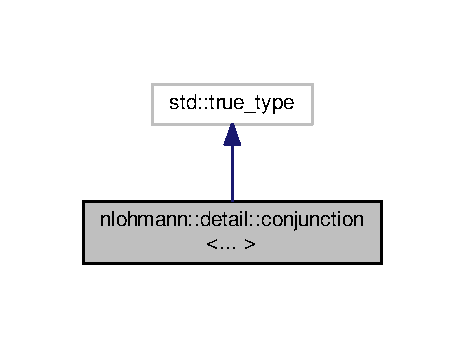
\includegraphics[width=223pt]{structnlohmann_1_1detail_1_1conjunction__inherit__graph}
\end{center}
\end{figure}


Collaboration diagram for nlohmann\+:\+:detail\+:\+:conjunction$<$... $>$\+:
\nopagebreak
\begin{figure}[H]
\begin{center}
\leavevmode
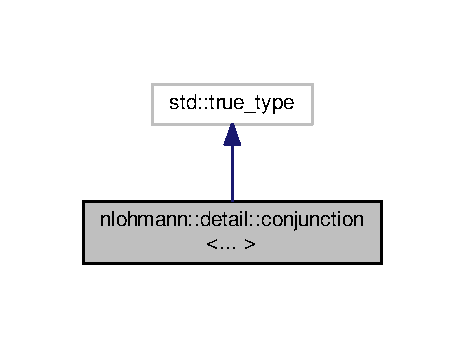
\includegraphics[width=223pt]{structnlohmann_1_1detail_1_1conjunction__coll__graph}
\end{center}
\end{figure}


The documentation for this struct was generated from the following file\+:\begin{DoxyCompactItemize}
\item 
json.\+hpp\end{DoxyCompactItemize}

\hypertarget{structnlohmann_1_1detail_1_1conjunction_3_01B1_01_4}{}\section{nlohmann\+:\+:detail\+:\+:conjunction$<$ B1 $>$ Struct Template Reference}
\label{structnlohmann_1_1detail_1_1conjunction_3_01B1_01_4}\index{nlohmann\+::detail\+::conjunction$<$ B1 $>$@{nlohmann\+::detail\+::conjunction$<$ B1 $>$}}


Inheritance diagram for nlohmann\+:\+:detail\+:\+:conjunction$<$ B1 $>$\+:
\nopagebreak
\begin{figure}[H]
\begin{center}
\leavevmode
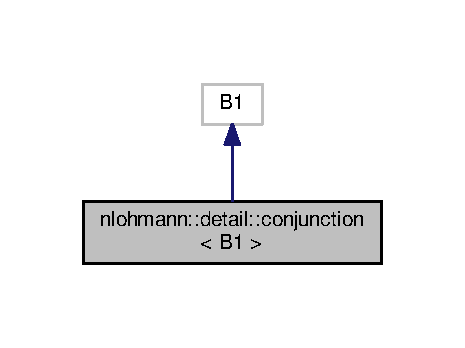
\includegraphics[width=223pt]{structnlohmann_1_1detail_1_1conjunction_3_01B1_01_4__inherit__graph}
\end{center}
\end{figure}


Collaboration diagram for nlohmann\+:\+:detail\+:\+:conjunction$<$ B1 $>$\+:
\nopagebreak
\begin{figure}[H]
\begin{center}
\leavevmode
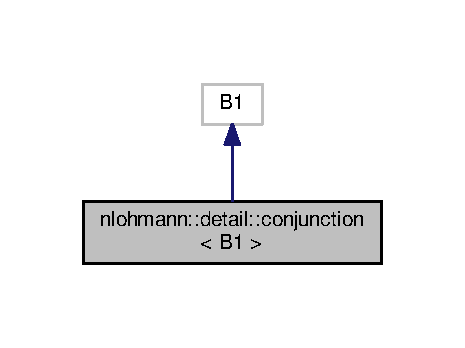
\includegraphics[width=223pt]{structnlohmann_1_1detail_1_1conjunction_3_01B1_01_4__coll__graph}
\end{center}
\end{figure}


The documentation for this struct was generated from the following file\+:\begin{DoxyCompactItemize}
\item 
json.\+hpp\end{DoxyCompactItemize}

\hypertarget{structnlohmann_1_1detail_1_1conjunction_3_01B1_00_01Bn_8_8_8_01_4}{}\section{nlohmann\+:\+:detail\+:\+:conjunction$<$ B1, Bn... $>$ Struct Template Reference}
\label{structnlohmann_1_1detail_1_1conjunction_3_01B1_00_01Bn_8_8_8_01_4}\index{nlohmann\+::detail\+::conjunction$<$ B1, Bn... $>$@{nlohmann\+::detail\+::conjunction$<$ B1, Bn... $>$}}


Inheritance diagram for nlohmann\+:\+:detail\+:\+:conjunction$<$ B1, Bn... $>$\+:
\nopagebreak
\begin{figure}[H]
\begin{center}
\leavevmode
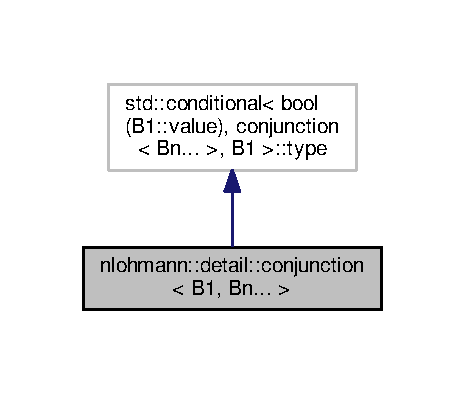
\includegraphics[width=223pt]{structnlohmann_1_1detail_1_1conjunction_3_01B1_00_01Bn_8_8_8_01_4__inherit__graph}
\end{center}
\end{figure}


Collaboration diagram for nlohmann\+:\+:detail\+:\+:conjunction$<$ B1, Bn... $>$\+:
\nopagebreak
\begin{figure}[H]
\begin{center}
\leavevmode
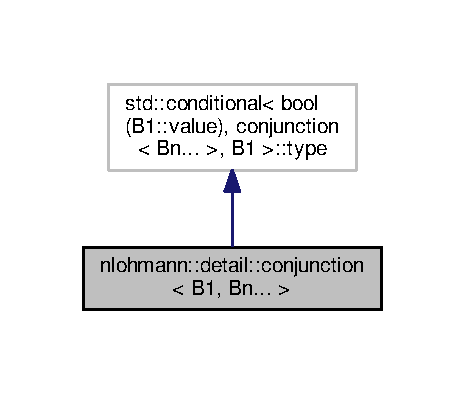
\includegraphics[width=223pt]{structnlohmann_1_1detail_1_1conjunction_3_01B1_00_01Bn_8_8_8_01_4__coll__graph}
\end{center}
\end{figure}


The documentation for this struct was generated from the following file\+:\begin{DoxyCompactItemize}
\item 
json.\+hpp\end{DoxyCompactItemize}

\hypertarget{classCrocodillia}{}\section{Crocodillia Class Reference}
\label{classCrocodillia}\index{Crocodillia@{Crocodillia}}


{\ttfamily \#include $<$animal.\+h$>$}



Inheritance diagram for Crocodillia\+:
\nopagebreak
\begin{figure}[H]
\begin{center}
\leavevmode
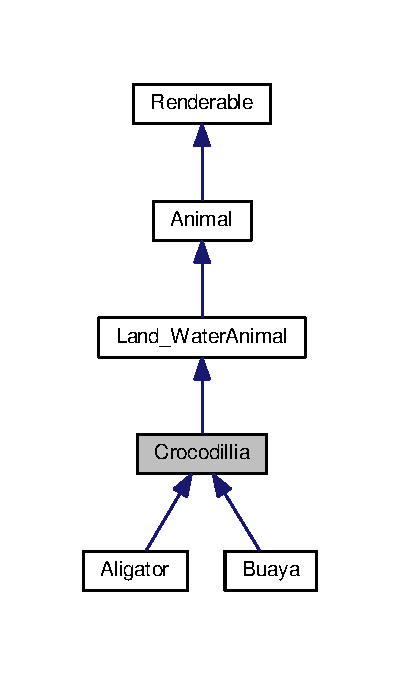
\includegraphics[width=192pt]{classCrocodillia__inherit__graph}
\end{center}
\end{figure}


Collaboration diagram for Crocodillia\+:
\nopagebreak
\begin{figure}[H]
\begin{center}
\leavevmode
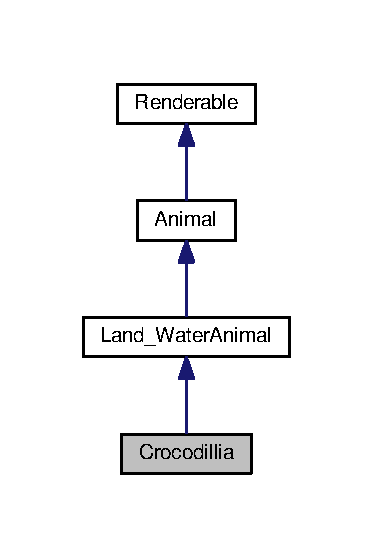
\includegraphics[width=179pt]{classCrocodillia__coll__graph}
\end{center}
\end{figure}
\subsection*{Public Member Functions}
\begin{DoxyCompactItemize}
\item 
\hyperlink{classCrocodillia_a98a15dfd88ad4799bfaaf849d0692176}{Crocodillia} (char c, int i)
\begin{DoxyCompactList}\small\item\em Constructor. Menciptakan Crocodilla dengan memanggil constructor \hyperlink{classLand__WaterAnimal}{Land\+\_\+\+Water\+Animal} berinisial c dan ID i. \end{DoxyCompactList}\end{DoxyCompactItemize}
\subsection*{Additional Inherited Members}


\subsection{Detailed Description}
Kelas \hyperlink{classCrocodillia}{Crocodillia} turunan dari \hyperlink{classLand__WaterAnimal}{Land\+\_\+\+Water\+Animal} 

\subsection{Constructor \& Destructor Documentation}
\index{Crocodillia@{Crocodillia}!Crocodillia@{Crocodillia}}
\index{Crocodillia@{Crocodillia}!Crocodillia@{Crocodillia}}
\subsubsection[{\texorpdfstring{Crocodillia(char c, int i)}{Crocodillia(char c, int i)}}]{\setlength{\rightskip}{0pt plus 5cm}Crocodillia\+::\+Crocodillia (
\begin{DoxyParamCaption}
\item[{char}]{c, }
\item[{int}]{i}
\end{DoxyParamCaption}
)}\hypertarget{classCrocodillia_a98a15dfd88ad4799bfaaf849d0692176}{}\label{classCrocodillia_a98a15dfd88ad4799bfaaf849d0692176}


Constructor. Menciptakan Crocodilla dengan memanggil constructor \hyperlink{classLand__WaterAnimal}{Land\+\_\+\+Water\+Animal} berinisial c dan ID i. 


\begin{DoxyParams}{Parameters}
{\em c} & inisial Crocodilla yang ingin diciptakan \\
\hline
{\em i} & ID Crocodilla yang ingin diciptakan \\
\hline
\end{DoxyParams}


The documentation for this class was generated from the following files\+:\begin{DoxyCompactItemize}
\item 
animal.\+h\item 
animal.\+cpp\end{DoxyCompactItemize}

\hypertarget{classDriver}{}\section{Driver Class Reference}
\label{classDriver}\index{Driver@{Driver}}


{\ttfamily \#include $<$driver.\+h$>$}

\subsection*{Public Member Functions}
\begin{DoxyCompactItemize}
\item 
\hyperlink{classDriver_af0658d103e3e810a8e9ef0a53bb2e261}{Driver} ()\hypertarget{classDriver_af0658d103e3e810a8e9ef0a53bb2e261}{}\label{classDriver_af0658d103e3e810a8e9ef0a53bb2e261}

\begin{DoxyCompactList}\small\item\em Constructor. Menciptakan kelas driver dengan informasi dari file eksternal. \end{DoxyCompactList}\item 
\hyperlink{classDriver_ac7645eea8d3ce2bc39ddbda5e840297a}{$\sim$\+Driver} ()\hypertarget{classDriver_ac7645eea8d3ce2bc39ddbda5e840297a}{}\label{classDriver_ac7645eea8d3ce2bc39ddbda5e840297a}

\begin{DoxyCompactList}\small\item\em Destructor. \end{DoxyCompactList}\item 
void \hyperlink{classDriver_a7beba85f4b72a9ce62b6be04585d7c06}{Init\+Zoo} (\hyperlink{classZoo}{Zoo} $\ast$$\ast$z, \hyperlink{classCageHandler}{Cage\+Handler} \&ch)
\begin{DoxyCompactList}\small\item\em Menginisiasi \hyperlink{classZoo}{Zoo} Membaca file eksternal dan membaca isinya untuk mengisi \hyperlink{classZoo}{Zoo}. \end{DoxyCompactList}\item 
void \hyperlink{classDriver_ac709deb2cb009df905c1be2fe33c9ba6}{Init\+Cage} (\hyperlink{classCageHandler}{Cage\+Handler} \&ch)
\begin{DoxyCompactList}\small\item\em Menginisiasi \hyperlink{classCage}{Cage} Membaca file eksternal dan membaca isinya untuk membuat cage. \end{DoxyCompactList}\item 
void \hyperlink{classDriver_a3d2d11d8f8e99ef2bfe8b55227a2b9cf}{Init\+Animal} (\hyperlink{classAnimalHandler}{Animal\+Handler} \&ah, \hyperlink{classZoo}{Zoo} \&z)
\begin{DoxyCompactList}\small\item\em Menginisiasi \hyperlink{classAnimal}{Animal} Membaca file eksternal dan membaca isinya untuk membuat animal. \end{DoxyCompactList}\item 
void \hyperlink{classDriver_a966c5449a7c49685a7c69a58697a8537}{Display\+Virtual\+Zoo} (\hyperlink{classZoo}{Zoo} \&)\hypertarget{classDriver_a966c5449a7c49685a7c69a58697a8537}{}\label{classDriver_a966c5449a7c49685a7c69a58697a8537}

\begin{DoxyCompactList}\small\item\em Menampilkan \hyperlink{classZoo}{Zoo} Menampilkan isi dari \hyperlink{classZoo}{Zoo} ke layar. \end{DoxyCompactList}\item 
void \hyperlink{classDriver_a31e7c4799004a705523115be083686ca}{Init\+Position} (\hyperlink{classZoo}{Zoo} \&)\hypertarget{classDriver_a31e7c4799004a705523115be083686ca}{}\label{classDriver_a31e7c4799004a705523115be083686ca}

\begin{DoxyCompactList}\small\item\em Menginisiasi posisi user di \hyperlink{classZoo}{Zoo} Menginisiasi curr\+\_\+x dan curr\+\_\+y secara random. \end{DoxyCompactList}\item 
int \hyperlink{classDriver_a4538dcc6da88490c3585c1937b809737}{Get\+PosX} ()
\begin{DoxyCompactList}\small\item\em Getter posisi x dari user. \end{DoxyCompactList}\item 
int \hyperlink{classDriver_af299632638b6c848bd6b47d632541982}{Get\+PosY} ()
\begin{DoxyCompactList}\small\item\em Getter posisi y dari user. \end{DoxyCompactList}\item 
void \hyperlink{classDriver_acadd7e79ec4ed26eb390ff2821afbaea}{Tour\+Virtual\+Zoo} (\hyperlink{classZoo}{Zoo} \&)\hypertarget{classDriver_acadd7e79ec4ed26eb390ff2821afbaea}{}\label{classDriver_acadd7e79ec4ed26eb390ff2821afbaea}

\begin{DoxyCompactList}\small\item\em Melakukan tour dalam \hyperlink{classZoo}{Zoo} Memindahkan posisi x dan y dari user sesuai jalan di zoo Menampilkan setiap interaksi dengan animal yang dilalui saat tour. \end{DoxyCompactList}\item 
void \hyperlink{classDriver_a3a17437e65824c453001d5b16def3508}{Move\+Animal} (\hyperlink{classZoo}{Zoo} \&z, \hyperlink{classAnimalHandler}{Animal\+Handler} \&ah)
\begin{DoxyCompactList}\small\item\em Memindahkan posisi animal. \end{DoxyCompactList}\end{DoxyCompactItemize}


\subsection{Detailed Description}
Kelas \hyperlink{classDriver}{Driver} berfungsi menginisiasi Program Utama 

\subsection{Member Function Documentation}
\index{Driver@{Driver}!Get\+PosX@{Get\+PosX}}
\index{Get\+PosX@{Get\+PosX}!Driver@{Driver}}
\subsubsection[{\texorpdfstring{Get\+Pos\+X()}{GetPosX()}}]{\setlength{\rightskip}{0pt plus 5cm}int Driver\+::\+Get\+PosX (
\begin{DoxyParamCaption}
{}
\end{DoxyParamCaption}
)}\hypertarget{classDriver_a4538dcc6da88490c3585c1937b809737}{}\label{classDriver_a4538dcc6da88490c3585c1937b809737}


Getter posisi x dari user. 

\begin{DoxyReturn}{Returns}
curr\+\_\+x 
\end{DoxyReturn}
\index{Driver@{Driver}!Get\+PosY@{Get\+PosY}}
\index{Get\+PosY@{Get\+PosY}!Driver@{Driver}}
\subsubsection[{\texorpdfstring{Get\+Pos\+Y()}{GetPosY()}}]{\setlength{\rightskip}{0pt plus 5cm}int Driver\+::\+Get\+PosY (
\begin{DoxyParamCaption}
{}
\end{DoxyParamCaption}
)}\hypertarget{classDriver_af299632638b6c848bd6b47d632541982}{}\label{classDriver_af299632638b6c848bd6b47d632541982}


Getter posisi y dari user. 

\begin{DoxyReturn}{Returns}
curr\+\_\+y 
\end{DoxyReturn}
\index{Driver@{Driver}!Init\+Animal@{Init\+Animal}}
\index{Init\+Animal@{Init\+Animal}!Driver@{Driver}}
\subsubsection[{\texorpdfstring{Init\+Animal(\+Animal\+Handler \&ah, Zoo \&z)}{InitAnimal(AnimalHandler &ah, Zoo &z)}}]{\setlength{\rightskip}{0pt plus 5cm}void Driver\+::\+Init\+Animal (
\begin{DoxyParamCaption}
\item[{{\bf Animal\+Handler} \&}]{ah, }
\item[{{\bf Zoo} \&}]{z}
\end{DoxyParamCaption}
)}\hypertarget{classDriver_a3d2d11d8f8e99ef2bfe8b55227a2b9cf}{}\label{classDriver_a3d2d11d8f8e99ef2bfe8b55227a2b9cf}


Menginisiasi \hyperlink{classAnimal}{Animal} Membaca file eksternal dan membaca isinya untuk membuat animal. 


\begin{DoxyParams}{Parameters}
{\em ah} & \hyperlink{classAnimalHandler}{Animal\+Handler} yang diisi oleh animal \\
\hline
{\em z} & \hyperlink{classZoo}{Zoo} yang akan diisi oleh animal \\
\hline
\end{DoxyParams}
\index{Driver@{Driver}!Init\+Cage@{Init\+Cage}}
\index{Init\+Cage@{Init\+Cage}!Driver@{Driver}}
\subsubsection[{\texorpdfstring{Init\+Cage(\+Cage\+Handler \&ch)}{InitCage(CageHandler &ch)}}]{\setlength{\rightskip}{0pt plus 5cm}void Driver\+::\+Init\+Cage (
\begin{DoxyParamCaption}
\item[{{\bf Cage\+Handler} \&}]{ch}
\end{DoxyParamCaption}
)}\hypertarget{classDriver_ac709deb2cb009df905c1be2fe33c9ba6}{}\label{classDriver_ac709deb2cb009df905c1be2fe33c9ba6}


Menginisiasi \hyperlink{classCage}{Cage} Membaca file eksternal dan membaca isinya untuk membuat cage. 


\begin{DoxyParams}{Parameters}
{\em ch} & \hyperlink{classCageHandler}{Cage\+Handler} yang diisi oleh cage \\
\hline
\end{DoxyParams}
\index{Driver@{Driver}!Init\+Zoo@{Init\+Zoo}}
\index{Init\+Zoo@{Init\+Zoo}!Driver@{Driver}}
\subsubsection[{\texorpdfstring{Init\+Zoo(\+Zoo $\ast$$\ast$z, Cage\+Handler \&ch)}{InitZoo(Zoo **z, CageHandler &ch)}}]{\setlength{\rightskip}{0pt plus 5cm}void Driver\+::\+Init\+Zoo (
\begin{DoxyParamCaption}
\item[{{\bf Zoo} $\ast$$\ast$}]{z, }
\item[{{\bf Cage\+Handler} \&}]{ch}
\end{DoxyParamCaption}
)}\hypertarget{classDriver_a7beba85f4b72a9ce62b6be04585d7c06}{}\label{classDriver_a7beba85f4b72a9ce62b6be04585d7c06}


Menginisiasi \hyperlink{classZoo}{Zoo} Membaca file eksternal dan membaca isinya untuk mengisi \hyperlink{classZoo}{Zoo}. 


\begin{DoxyParams}{Parameters}
{\em z} & Kelas \hyperlink{classZoo}{Zoo} yang akan diciptakan \\
\hline
{\em ch} & \hyperlink{classCageHandler}{Cage\+Handler} yang setiap cagenya akan diisi cell \\
\hline
\end{DoxyParams}
\index{Driver@{Driver}!Move\+Animal@{Move\+Animal}}
\index{Move\+Animal@{Move\+Animal}!Driver@{Driver}}
\subsubsection[{\texorpdfstring{Move\+Animal(\+Zoo \&z, Animal\+Handler \&ah)}{MoveAnimal(Zoo &z, AnimalHandler &ah)}}]{\setlength{\rightskip}{0pt plus 5cm}void Driver\+::\+Move\+Animal (
\begin{DoxyParamCaption}
\item[{{\bf Zoo} \&}]{z, }
\item[{{\bf Animal\+Handler} \&}]{ah}
\end{DoxyParamCaption}
)}\hypertarget{classDriver_a3a17437e65824c453001d5b16def3508}{}\label{classDriver_a3a17437e65824c453001d5b16def3508}


Memindahkan posisi animal. 


\begin{DoxyParams}{Parameters}
{\em z} & \hyperlink{classZoo}{Zoo} yang animalnya akan dipindahkan \\
\hline
{\em ah} & list dari semua animal \\
\hline
\end{DoxyParams}


The documentation for this class was generated from the following files\+:\begin{DoxyCompactItemize}
\item 
driver.\+h\item 
driver.\+cpp\end{DoxyCompactItemize}

\hypertarget{classElang}{}\section{Elang Class Reference}
\label{classElang}\index{Elang@{Elang}}


{\ttfamily \#include $<$listanimal.\+h$>$}



Inheritance diagram for Elang\+:
\nopagebreak
\begin{figure}[H]
\begin{center}
\leavevmode
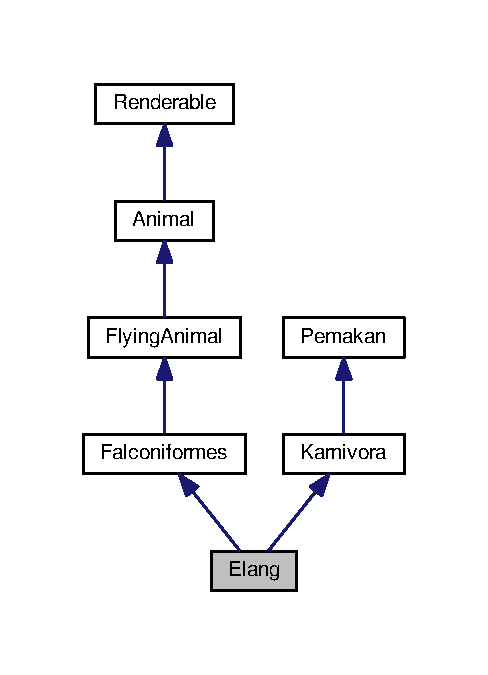
\includegraphics[width=234pt]{classElang__inherit__graph}
\end{center}
\end{figure}


Collaboration diagram for Elang\+:
\nopagebreak
\begin{figure}[H]
\begin{center}
\leavevmode
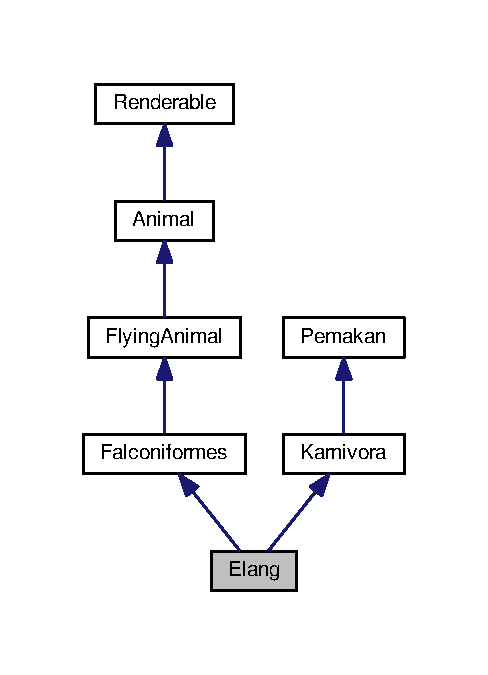
\includegraphics[width=234pt]{classElang__coll__graph}
\end{center}
\end{figure}
\subsection*{Public Member Functions}
\begin{DoxyCompactItemize}
\item 
\hyperlink{classElang_a0498b01d6007cf95ea065322a4ef87fa}{Elang} (int i, int x, int y, int massa, bool jinak)
\begin{DoxyCompactList}\small\item\em Constructor. Menciptakan \hyperlink{classElang}{Elang} dengan inisial \textquotesingle{}$\sim$\textquotesingle{} dan ID i. \end{DoxyCompactList}\item 
void \hyperlink{classElang_a0ab640b797d57d2a7068eb062bd81806}{Interact} ()\hypertarget{classElang_a0ab640b797d57d2a7068eb062bd81806}{}\label{classElang_a0ab640b797d57d2a7068eb062bd81806}

\begin{DoxyCompactList}\small\item\em Menampilkan suara binatang ke layar. \end{DoxyCompactList}\item 
int \hyperlink{classElang_a6d017711dba92202dfad0126d636a28a}{Get\+Jml\+Makanan} ()
\begin{DoxyCompactList}\small\item\em Melihat jumlah makanan dari binatang. Memanggil fungsi Get\+Amount parent Karivora. \end{DoxyCompactList}\end{DoxyCompactItemize}
\subsection*{Additional Inherited Members}


\subsection{Detailed Description}
Kelas \hyperlink{classElang}{Elang} turunan dari \hyperlink{classFalconiformes}{Falconiformes} dan \hyperlink{classKarnivora}{Karnivora} 

\subsection{Constructor \& Destructor Documentation}
\index{Elang@{Elang}!Elang@{Elang}}
\index{Elang@{Elang}!Elang@{Elang}}
\subsubsection[{\texorpdfstring{Elang(int i, int x, int y, int massa, bool jinak)}{Elang(int i, int x, int y, int massa, bool jinak)}}]{\setlength{\rightskip}{0pt plus 5cm}Elang\+::\+Elang (
\begin{DoxyParamCaption}
\item[{int}]{i, }
\item[{int}]{x, }
\item[{int}]{y, }
\item[{int}]{massa, }
\item[{bool}]{jinak}
\end{DoxyParamCaption}
)}\hypertarget{classElang_a0498b01d6007cf95ea065322a4ef87fa}{}\label{classElang_a0498b01d6007cf95ea065322a4ef87fa}


Constructor. Menciptakan \hyperlink{classElang}{Elang} dengan inisial \textquotesingle{}$\sim$\textquotesingle{} dan ID i. 


\begin{DoxyParams}{Parameters}
{\em i} & Nilai Id \hyperlink{classAnimal}{Animal} yang diciptakan \\
\hline
{\em x} & Posisi x \hyperlink{classAnimal}{Animal} yang diciptakan \\
\hline
{\em y} & Posisi y \hyperlink{classAnimal}{Animal} yang diciptakan \\
\hline
{\em massa} & berat \hyperlink{classAnimal}{Animal} yang diciptakan \\
\hline
{\em jinak} & nilai jinak \hyperlink{classAnimal}{Animal} yang diciptakan \\
\hline
\end{DoxyParams}


\subsection{Member Function Documentation}
\index{Elang@{Elang}!Get\+Jml\+Makanan@{Get\+Jml\+Makanan}}
\index{Get\+Jml\+Makanan@{Get\+Jml\+Makanan}!Elang@{Elang}}
\subsubsection[{\texorpdfstring{Get\+Jml\+Makanan()}{GetJmlMakanan()}}]{\setlength{\rightskip}{0pt plus 5cm}int Elang\+::\+Get\+Jml\+Makanan (
\begin{DoxyParamCaption}
{}
\end{DoxyParamCaption}
)\hspace{0.3cm}{\ttfamily [virtual]}}\hypertarget{classElang_a6d017711dba92202dfad0126d636a28a}{}\label{classElang_a6d017711dba92202dfad0126d636a28a}


Melihat jumlah makanan dari binatang. Memanggil fungsi Get\+Amount parent Karivora. 

\begin{DoxyReturn}{Returns}
Jumlah makanan dari binatang. 
\end{DoxyReturn}


Implements \hyperlink{classAnimal_a3f1cced7bac93f7c88a24ec5a0e989fe}{Animal}.



The documentation for this class was generated from the following files\+:\begin{DoxyCompactItemize}
\item 
listanimal.\+h\item 
listanimal.\+cpp\end{DoxyCompactItemize}

\hypertarget{classEntrance}{}\section{Entrance Class Reference}
\label{classEntrance}\index{Entrance@{Entrance}}


{\ttfamily \#include $<$zoo.\+h$>$}



Inheritance diagram for Entrance\+:
\nopagebreak
\begin{figure}[H]
\begin{center}
\leavevmode
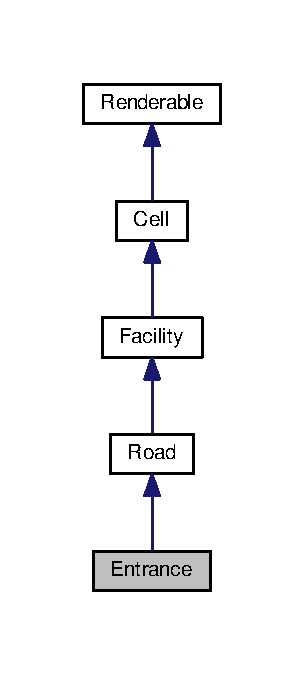
\includegraphics[width=146pt]{classEntrance__inherit__graph}
\end{center}
\end{figure}


Collaboration diagram for Entrance\+:
\nopagebreak
\begin{figure}[H]
\begin{center}
\leavevmode
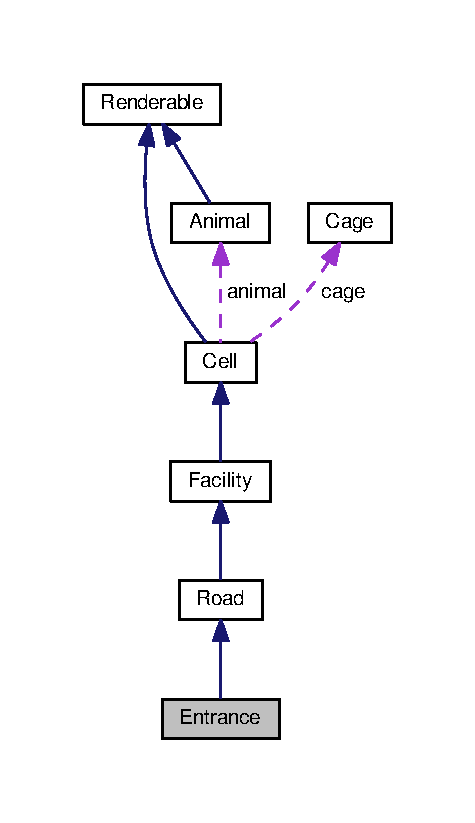
\includegraphics[width=228pt]{classEntrance__coll__graph}
\end{center}
\end{figure}
\subsection*{Public Member Functions}
\begin{DoxyCompactItemize}
\item 
\hyperlink{classEntrance_acfb8b9f5d174b102562ee8989b8e20d4}{Entrance} (int x, int y)
\begin{DoxyCompactList}\small\item\em Constructor Menciptakan \hyperlink{classEntrance}{Entrance} dengan memanggil constructor \hyperlink{classRoad}{Road} yang memiliki posisi $<$x,y$>$ \end{DoxyCompactList}\end{DoxyCompactItemize}
\subsection*{Additional Inherited Members}


\subsection{Detailed Description}
Kelas \hyperlink{classEntrance}{Entrance} inherit dari kelas \hyperlink{classRoad}{Road}, sebagai tempat masuk \hyperlink{classZoo}{Zoo} 

\subsection{Constructor \& Destructor Documentation}
\index{Entrance@{Entrance}!Entrance@{Entrance}}
\index{Entrance@{Entrance}!Entrance@{Entrance}}
\subsubsection[{\texorpdfstring{Entrance(int x, int y)}{Entrance(int x, int y)}}]{\setlength{\rightskip}{0pt plus 5cm}Entrance\+::\+Entrance (
\begin{DoxyParamCaption}
\item[{int}]{x, }
\item[{int}]{y}
\end{DoxyParamCaption}
)}\hypertarget{classEntrance_acfb8b9f5d174b102562ee8989b8e20d4}{}\label{classEntrance_acfb8b9f5d174b102562ee8989b8e20d4}


Constructor Menciptakan \hyperlink{classEntrance}{Entrance} dengan memanggil constructor \hyperlink{classRoad}{Road} yang memiliki posisi $<$x,y$>$ 


\begin{DoxyParams}{Parameters}
{\em x} & Nilai absis \hyperlink{classRoad}{Road} yang diciptakan \\
\hline
{\em y} & Nilai ordinat \hyperlink{classRoad}{Road} yang diciptakan \\
\hline
\end{DoxyParams}


The documentation for this class was generated from the following files\+:\begin{DoxyCompactItemize}
\item 
zoo.\+h\item 
zoo.\+cpp\end{DoxyCompactItemize}

\hypertarget{classExit}{}\section{Exit Class Reference}
\label{classExit}\index{Exit@{Exit}}


{\ttfamily \#include $<$zoo.\+h$>$}



Inheritance diagram for Exit\+:
\nopagebreak
\begin{figure}[H]
\begin{center}
\leavevmode
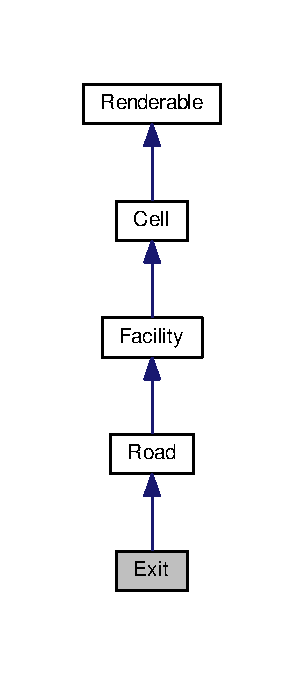
\includegraphics[width=146pt]{classExit__inherit__graph}
\end{center}
\end{figure}


Collaboration diagram for Exit\+:
\nopagebreak
\begin{figure}[H]
\begin{center}
\leavevmode
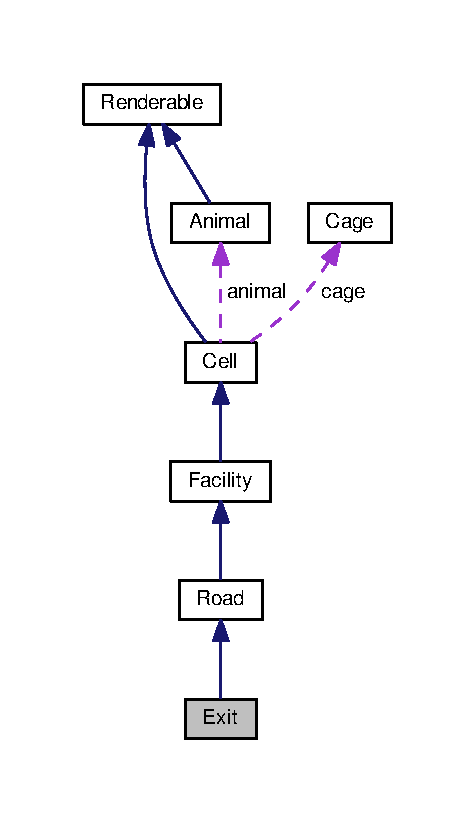
\includegraphics[width=228pt]{classExit__coll__graph}
\end{center}
\end{figure}
\subsection*{Public Member Functions}
\begin{DoxyCompactItemize}
\item 
\hyperlink{classExit_abb37d76b2e66fac8cac92fd61dfee563}{Exit} (int x, int y)
\begin{DoxyCompactList}\small\item\em Constructor Menciptakan \hyperlink{classExit}{Exit} dengan memanggil constructor \hyperlink{classRoad}{Road} yang memiliki posisi $<$x,y$>$ \end{DoxyCompactList}\end{DoxyCompactItemize}
\subsection*{Additional Inherited Members}


\subsection{Detailed Description}
Kelas \hyperlink{classExit}{Exit} inherit dari kelas \hyperlink{classRoad}{Road}, sebagai tempat keluar \hyperlink{classZoo}{Zoo} 

\subsection{Constructor \& Destructor Documentation}
\index{Exit@{Exit}!Exit@{Exit}}
\index{Exit@{Exit}!Exit@{Exit}}
\subsubsection[{\texorpdfstring{Exit(int x, int y)}{Exit(int x, int y)}}]{\setlength{\rightskip}{0pt plus 5cm}Exit\+::\+Exit (
\begin{DoxyParamCaption}
\item[{int}]{x, }
\item[{int}]{y}
\end{DoxyParamCaption}
)}\hypertarget{classExit_abb37d76b2e66fac8cac92fd61dfee563}{}\label{classExit_abb37d76b2e66fac8cac92fd61dfee563}


Constructor Menciptakan \hyperlink{classExit}{Exit} dengan memanggil constructor \hyperlink{classRoad}{Road} yang memiliki posisi $<$x,y$>$ 


\begin{DoxyParams}{Parameters}
{\em x} & Nilai absis \hyperlink{classRoad}{Road} yang diciptakan \\
\hline
{\em y} & Nilai ordinat \hyperlink{classRoad}{Road} yang diciptakan \\
\hline
\end{DoxyParams}


The documentation for this class was generated from the following files\+:\begin{DoxyCompactItemize}
\item 
zoo.\+h\item 
zoo.\+cpp\end{DoxyCompactItemize}

\hypertarget{structnlohmann_1_1detail_1_1external__constructor}{}\section{nlohmann\+:\+:detail\+:\+:external\+\_\+constructor$<$ value\+\_\+t $>$ Struct Template Reference}
\label{structnlohmann_1_1detail_1_1external__constructor}\index{nlohmann\+::detail\+::external\+\_\+constructor$<$ value\+\_\+t $>$@{nlohmann\+::detail\+::external\+\_\+constructor$<$ value\+\_\+t $>$}}


The documentation for this struct was generated from the following file\+:\begin{DoxyCompactItemize}
\item 
json.\+hpp\end{DoxyCompactItemize}

\hypertarget{structnlohmann_1_1detail_1_1external__constructor_3_01value__t_1_1array_01_4}{}\section{nlohmann\+:\+:detail\+:\+:external\+\_\+constructor$<$ value\+\_\+t\+:\+:array $>$ Struct Template Reference}
\label{structnlohmann_1_1detail_1_1external__constructor_3_01value__t_1_1array_01_4}\index{nlohmann\+::detail\+::external\+\_\+constructor$<$ value\+\_\+t\+::array $>$@{nlohmann\+::detail\+::external\+\_\+constructor$<$ value\+\_\+t\+::array $>$}}
\subsection*{Static Public Member Functions}
\begin{DoxyCompactItemize}
\item 
{\footnotesize template$<$typename Basic\+Json\+Type $>$ }\\static void {\bfseries construct} (Basic\+Json\+Type \&j, const typename Basic\+Json\+Type\+::array\+\_\+t \&arr)\hypertarget{structnlohmann_1_1detail_1_1external__constructor_3_01value__t_1_1array_01_4_abfb2a6eec0bc21e8a7438546aebc55d8}{}\label{structnlohmann_1_1detail_1_1external__constructor_3_01value__t_1_1array_01_4_abfb2a6eec0bc21e8a7438546aebc55d8}

\item 
{\footnotesize template$<$typename Basic\+Json\+Type , typename Compatible\+Array\+Type , enable\+\_\+if\+\_\+t$<$ not std\+::is\+\_\+same$<$ Compatible\+Array\+Type, typename Basic\+Json\+Type\+::array\+\_\+t $>$\+::value, int $>$  = 0$>$ }\\static void {\bfseries construct} (Basic\+Json\+Type \&j, const Compatible\+Array\+Type \&arr)\hypertarget{structnlohmann_1_1detail_1_1external__constructor_3_01value__t_1_1array_01_4_a110f50fd5378da876d9a6d6a8d945e37}{}\label{structnlohmann_1_1detail_1_1external__constructor_3_01value__t_1_1array_01_4_a110f50fd5378da876d9a6d6a8d945e37}

\end{DoxyCompactItemize}


The documentation for this struct was generated from the following file\+:\begin{DoxyCompactItemize}
\item 
json.\+hpp\end{DoxyCompactItemize}

\hypertarget{structnlohmann_1_1detail_1_1external__constructor_3_01value__t_1_1boolean_01_4}{}\section{nlohmann\+:\+:detail\+:\+:external\+\_\+constructor$<$ value\+\_\+t\+:\+:boolean $>$ Struct Template Reference}
\label{structnlohmann_1_1detail_1_1external__constructor_3_01value__t_1_1boolean_01_4}\index{nlohmann\+::detail\+::external\+\_\+constructor$<$ value\+\_\+t\+::boolean $>$@{nlohmann\+::detail\+::external\+\_\+constructor$<$ value\+\_\+t\+::boolean $>$}}
\subsection*{Static Public Member Functions}
\begin{DoxyCompactItemize}
\item 
{\footnotesize template$<$typename Basic\+Json\+Type $>$ }\\static void {\bfseries construct} (Basic\+Json\+Type \&j, typename Basic\+Json\+Type\+::boolean\+\_\+t b) noexcept\hypertarget{structnlohmann_1_1detail_1_1external__constructor_3_01value__t_1_1boolean_01_4_a867122bcf0856c757bd6bcbfb8be74bc}{}\label{structnlohmann_1_1detail_1_1external__constructor_3_01value__t_1_1boolean_01_4_a867122bcf0856c757bd6bcbfb8be74bc}

\end{DoxyCompactItemize}


The documentation for this struct was generated from the following file\+:\begin{DoxyCompactItemize}
\item 
json.\+hpp\end{DoxyCompactItemize}

\hypertarget{structnlohmann_1_1detail_1_1external__constructor_3_01value__t_1_1number__float_01_4}{}\section{nlohmann\+:\+:detail\+:\+:external\+\_\+constructor$<$ value\+\_\+t\+:\+:number\+\_\+float $>$ Struct Template Reference}
\label{structnlohmann_1_1detail_1_1external__constructor_3_01value__t_1_1number__float_01_4}\index{nlohmann\+::detail\+::external\+\_\+constructor$<$ value\+\_\+t\+::number\+\_\+float $>$@{nlohmann\+::detail\+::external\+\_\+constructor$<$ value\+\_\+t\+::number\+\_\+float $>$}}
\subsection*{Static Public Member Functions}
\begin{DoxyCompactItemize}
\item 
{\footnotesize template$<$typename Basic\+Json\+Type $>$ }\\static void {\bfseries construct} (Basic\+Json\+Type \&j, typename Basic\+Json\+Type\+::number\+\_\+float\+\_\+t val) noexcept\hypertarget{structnlohmann_1_1detail_1_1external__constructor_3_01value__t_1_1number__float_01_4_a669df5a4d258b588e67f747c6d656cdb}{}\label{structnlohmann_1_1detail_1_1external__constructor_3_01value__t_1_1number__float_01_4_a669df5a4d258b588e67f747c6d656cdb}

\end{DoxyCompactItemize}


The documentation for this struct was generated from the following file\+:\begin{DoxyCompactItemize}
\item 
json.\+hpp\end{DoxyCompactItemize}

\hypertarget{structnlohmann_1_1detail_1_1external__constructor_3_01value__t_1_1number__integer_01_4}{}\section{nlohmann\+:\+:detail\+:\+:external\+\_\+constructor$<$ value\+\_\+t\+:\+:number\+\_\+integer $>$ Struct Template Reference}
\label{structnlohmann_1_1detail_1_1external__constructor_3_01value__t_1_1number__integer_01_4}\index{nlohmann\+::detail\+::external\+\_\+constructor$<$ value\+\_\+t\+::number\+\_\+integer $>$@{nlohmann\+::detail\+::external\+\_\+constructor$<$ value\+\_\+t\+::number\+\_\+integer $>$}}
\subsection*{Static Public Member Functions}
\begin{DoxyCompactItemize}
\item 
{\footnotesize template$<$typename Basic\+Json\+Type $>$ }\\static void {\bfseries construct} (Basic\+Json\+Type \&j, typename Basic\+Json\+Type\+::number\+\_\+integer\+\_\+t val) noexcept\hypertarget{structnlohmann_1_1detail_1_1external__constructor_3_01value__t_1_1number__integer_01_4_a7c3949672ddb45095cc2527635feef0b}{}\label{structnlohmann_1_1detail_1_1external__constructor_3_01value__t_1_1number__integer_01_4_a7c3949672ddb45095cc2527635feef0b}

\end{DoxyCompactItemize}


The documentation for this struct was generated from the following file\+:\begin{DoxyCompactItemize}
\item 
json.\+hpp\end{DoxyCompactItemize}

\hypertarget{structnlohmann_1_1detail_1_1external__constructor_3_01value__t_1_1number__unsigned_01_4}{}\section{nlohmann\+:\+:detail\+:\+:external\+\_\+constructor$<$ value\+\_\+t\+:\+:number\+\_\+unsigned $>$ Struct Template Reference}
\label{structnlohmann_1_1detail_1_1external__constructor_3_01value__t_1_1number__unsigned_01_4}\index{nlohmann\+::detail\+::external\+\_\+constructor$<$ value\+\_\+t\+::number\+\_\+unsigned $>$@{nlohmann\+::detail\+::external\+\_\+constructor$<$ value\+\_\+t\+::number\+\_\+unsigned $>$}}
\subsection*{Static Public Member Functions}
\begin{DoxyCompactItemize}
\item 
{\footnotesize template$<$typename Basic\+Json\+Type $>$ }\\static void {\bfseries construct} (Basic\+Json\+Type \&j, typename Basic\+Json\+Type\+::number\+\_\+unsigned\+\_\+t val) noexcept\hypertarget{structnlohmann_1_1detail_1_1external__constructor_3_01value__t_1_1number__unsigned_01_4_a17969b14852f43e04353858c87b0f539}{}\label{structnlohmann_1_1detail_1_1external__constructor_3_01value__t_1_1number__unsigned_01_4_a17969b14852f43e04353858c87b0f539}

\end{DoxyCompactItemize}


The documentation for this struct was generated from the following file\+:\begin{DoxyCompactItemize}
\item 
json.\+hpp\end{DoxyCompactItemize}

\hypertarget{structnlohmann_1_1detail_1_1external__constructor_3_01value__t_1_1object_01_4}{}\section{nlohmann\+:\+:detail\+:\+:external\+\_\+constructor$<$ value\+\_\+t\+:\+:object $>$ Struct Template Reference}
\label{structnlohmann_1_1detail_1_1external__constructor_3_01value__t_1_1object_01_4}\index{nlohmann\+::detail\+::external\+\_\+constructor$<$ value\+\_\+t\+::object $>$@{nlohmann\+::detail\+::external\+\_\+constructor$<$ value\+\_\+t\+::object $>$}}
\subsection*{Static Public Member Functions}
\begin{DoxyCompactItemize}
\item 
{\footnotesize template$<$typename Basic\+Json\+Type $>$ }\\static void {\bfseries construct} (Basic\+Json\+Type \&j, const typename Basic\+Json\+Type\+::object\+\_\+t \&obj)\hypertarget{structnlohmann_1_1detail_1_1external__constructor_3_01value__t_1_1object_01_4_a3a369c5d49596dd4411e368425f9ac7a}{}\label{structnlohmann_1_1detail_1_1external__constructor_3_01value__t_1_1object_01_4_a3a369c5d49596dd4411e368425f9ac7a}

\item 
{\footnotesize template$<$typename Basic\+Json\+Type , typename Compatible\+Object\+Type , enable\+\_\+if\+\_\+t$<$ not std\+::is\+\_\+same$<$ Compatible\+Object\+Type, typename Basic\+Json\+Type\+::object\+\_\+t $>$\+::value, int $>$  = 0$>$ }\\static void {\bfseries construct} (Basic\+Json\+Type \&j, const Compatible\+Object\+Type \&obj)\hypertarget{structnlohmann_1_1detail_1_1external__constructor_3_01value__t_1_1object_01_4_a91f89abe0ec4dec59099b691682ff927}{}\label{structnlohmann_1_1detail_1_1external__constructor_3_01value__t_1_1object_01_4_a91f89abe0ec4dec59099b691682ff927}

\end{DoxyCompactItemize}


The documentation for this struct was generated from the following file\+:\begin{DoxyCompactItemize}
\item 
json.\+hpp\end{DoxyCompactItemize}

\hypertarget{structnlohmann_1_1detail_1_1external__constructor_3_01value__t_1_1string_01_4}{}\section{nlohmann\+:\+:detail\+:\+:external\+\_\+constructor$<$ value\+\_\+t\+:\+:string $>$ Struct Template Reference}
\label{structnlohmann_1_1detail_1_1external__constructor_3_01value__t_1_1string_01_4}\index{nlohmann\+::detail\+::external\+\_\+constructor$<$ value\+\_\+t\+::string $>$@{nlohmann\+::detail\+::external\+\_\+constructor$<$ value\+\_\+t\+::string $>$}}
\subsection*{Static Public Member Functions}
\begin{DoxyCompactItemize}
\item 
{\footnotesize template$<$typename Basic\+Json\+Type $>$ }\\static void {\bfseries construct} (Basic\+Json\+Type \&j, const typename Basic\+Json\+Type\+::string\+\_\+t \&s)\hypertarget{structnlohmann_1_1detail_1_1external__constructor_3_01value__t_1_1string_01_4_ad88d0b4b7ea01ea20e12cc1b82fe0d92}{}\label{structnlohmann_1_1detail_1_1external__constructor_3_01value__t_1_1string_01_4_ad88d0b4b7ea01ea20e12cc1b82fe0d92}

\end{DoxyCompactItemize}


The documentation for this struct was generated from the following file\+:\begin{DoxyCompactItemize}
\item 
json.\+hpp\end{DoxyCompactItemize}

\hypertarget{classFacility}{}\section{Facility Class Reference}
\label{classFacility}\index{Facility@{Facility}}


{\ttfamily \#include $<$zoo.\+h$>$}



Inheritance diagram for Facility\+:
\nopagebreak
\begin{figure}[H]
\begin{center}
\leavevmode
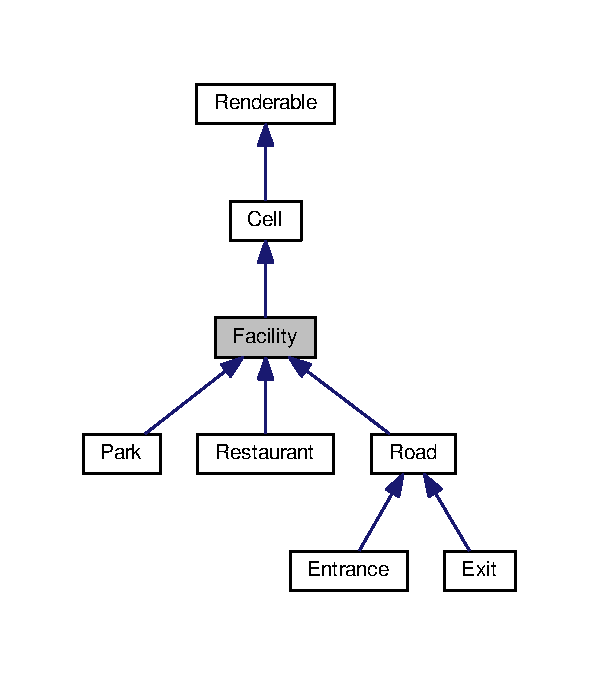
\includegraphics[width=288pt]{classFacility__inherit__graph}
\end{center}
\end{figure}


Collaboration diagram for Facility\+:
\nopagebreak
\begin{figure}[H]
\begin{center}
\leavevmode
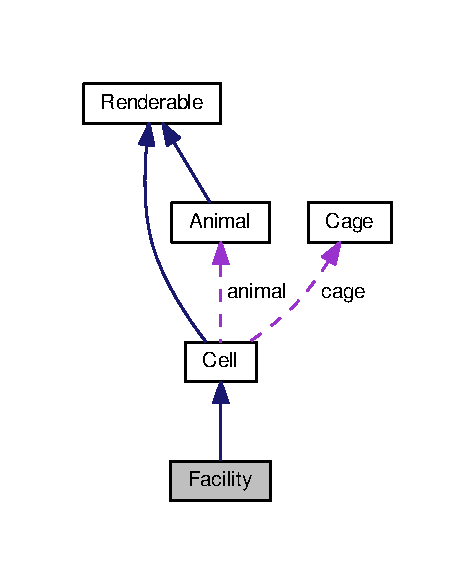
\includegraphics[width=228pt]{classFacility__coll__graph}
\end{center}
\end{figure}
\subsection*{Public Member Functions}
\begin{DoxyCompactItemize}
\item 
{\bfseries Facility} (char c, int x, int y)\hypertarget{classFacility_a33629884ce928c0d32ffd0509542af6f}{}\label{classFacility_a33629884ce928c0d32ffd0509542af6f}

\item 
virtual void \hyperlink{classFacility_a56a6c8fe31e61ca176db745931d5255b}{Render} ()\hypertarget{classFacility_a56a6c8fe31e61ca176db745931d5255b}{}\label{classFacility_a56a6c8fe31e61ca176db745931d5255b}

\begin{DoxyCompactList}\small\item\em Menampilkan type cell Menuliskan type dari cell ke layar. \end{DoxyCompactList}\end{DoxyCompactItemize}
\subsection*{Additional Inherited Members}


\subsection{Detailed Description}
Kelas \hyperlink{classFacility}{Facility} inherit dari kelas \hyperlink{classCell}{Cell}, merepresentasikan fasilitas zoo 

The documentation for this class was generated from the following files\+:\begin{DoxyCompactItemize}
\item 
zoo.\+h\item 
zoo.\+cpp\end{DoxyCompactItemize}

\hypertarget{classFalconformes}{}\section{Falconformes Class Reference}
\label{classFalconformes}\index{Falconformes@{Falconformes}}


{\ttfamily \#include $<$animal.\+h$>$}



\subsection{Detailed Description}
Kelas \hyperlink{classFalconformes}{Falconformes} turunan dari \hyperlink{classFlyingAnimal}{Flying\+Animal} 

The documentation for this class was generated from the following file\+:\begin{DoxyCompactItemize}
\item 
animal.\+h\end{DoxyCompactItemize}

\hypertarget{classFalconiformes}{}\section{Falconiformes Class Reference}
\label{classFalconiformes}\index{Falconiformes@{Falconiformes}}


Inheritance diagram for Falconiformes\+:
\nopagebreak
\begin{figure}[H]
\begin{center}
\leavevmode
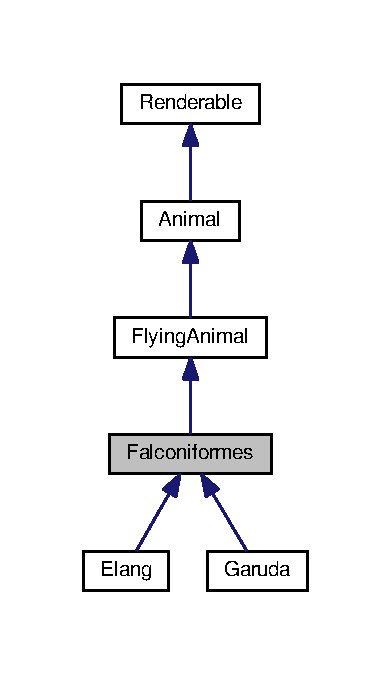
\includegraphics[width=188pt]{classFalconiformes__inherit__graph}
\end{center}
\end{figure}


Collaboration diagram for Falconiformes\+:
\nopagebreak
\begin{figure}[H]
\begin{center}
\leavevmode
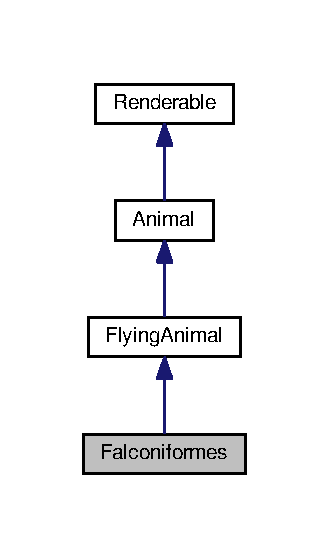
\includegraphics[width=158pt]{classFalconiformes__coll__graph}
\end{center}
\end{figure}
\subsection*{Public Member Functions}
\begin{DoxyCompactItemize}
\item 
\hyperlink{classFalconiformes_aff40437f58b5c172ac182f0b7c5e486c}{Falconiformes} (char c, int i)
\begin{DoxyCompactList}\small\item\em Constructor. Menciptakan \hyperlink{classFalconiformes}{Falconiformes} dengan memanggil constructor \hyperlink{classFlyingAnimal}{Flying\+Animal} berinisial c dan ID i. \end{DoxyCompactList}\end{DoxyCompactItemize}
\subsection*{Additional Inherited Members}


\subsection{Constructor \& Destructor Documentation}
\index{Falconiformes@{Falconiformes}!Falconiformes@{Falconiformes}}
\index{Falconiformes@{Falconiformes}!Falconiformes@{Falconiformes}}
\subsubsection[{\texorpdfstring{Falconiformes(char c, int i)}{Falconiformes(char c, int i)}}]{\setlength{\rightskip}{0pt plus 5cm}Falconiformes\+::\+Falconiformes (
\begin{DoxyParamCaption}
\item[{char}]{c, }
\item[{int}]{i}
\end{DoxyParamCaption}
)}\hypertarget{classFalconiformes_aff40437f58b5c172ac182f0b7c5e486c}{}\label{classFalconiformes_aff40437f58b5c172ac182f0b7c5e486c}


Constructor. Menciptakan \hyperlink{classFalconiformes}{Falconiformes} dengan memanggil constructor \hyperlink{classFlyingAnimal}{Flying\+Animal} berinisial c dan ID i. 


\begin{DoxyParams}{Parameters}
{\em c} & inisial \hyperlink{classFalconiformes}{Falconiformes} yang ingin diciptakan \\
\hline
{\em i} & ID \hyperlink{classFalconiformes}{Falconiformes} yang ingin diciptakan \\
\hline
\end{DoxyParams}


The documentation for this class was generated from the following files\+:\begin{DoxyCompactItemize}
\item 
animal.\+h\item 
animal.\+cpp\end{DoxyCompactItemize}

\hypertarget{classFlyingAnimal}{}\section{Flying\+Animal Class Reference}
\label{classFlyingAnimal}\index{Flying\+Animal@{Flying\+Animal}}


{\ttfamily \#include $<$animal.\+h$>$}



Inheritance diagram for Flying\+Animal\+:
\nopagebreak
\begin{figure}[H]
\begin{center}
\leavevmode
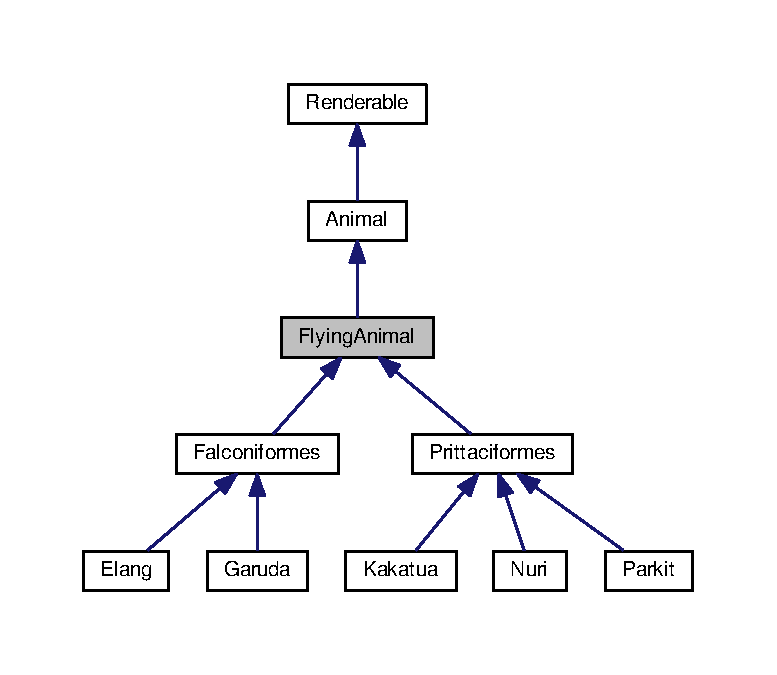
\includegraphics[width=350pt]{classFlyingAnimal__inherit__graph}
\end{center}
\end{figure}


Collaboration diagram for Flying\+Animal\+:
\nopagebreak
\begin{figure}[H]
\begin{center}
\leavevmode
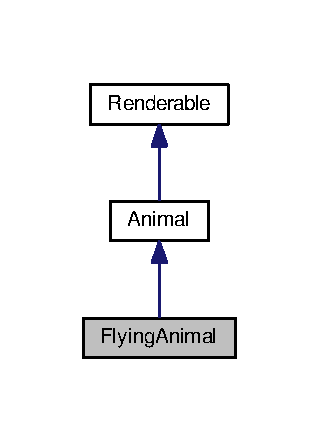
\includegraphics[width=153pt]{classFlyingAnimal__coll__graph}
\end{center}
\end{figure}
\subsection*{Public Member Functions}
\begin{DoxyCompactItemize}
\item 
\hyperlink{classFlyingAnimal_aaadfaeb6b44076a3434e909a2e3bb043}{Flying\+Animal} (char c, int i)
\begin{DoxyCompactList}\small\item\em Constructor. Menciptakan \hyperlink{classFlyingAnimal}{Flying\+Animal} dengan cara memanggil constructor \hyperlink{classAnimal}{Animal} berinisial c dan ID i. \end{DoxyCompactList}\end{DoxyCompactItemize}
\subsection*{Additional Inherited Members}


\subsection{Detailed Description}
Kelas \hyperlink{classFlyingAnimal}{Flying\+Animal} turunan dari \hyperlink{classAnimal}{Animal} menunjukkan animal yang tinggal di udara 

\subsection{Constructor \& Destructor Documentation}
\index{Flying\+Animal@{Flying\+Animal}!Flying\+Animal@{Flying\+Animal}}
\index{Flying\+Animal@{Flying\+Animal}!Flying\+Animal@{Flying\+Animal}}
\subsubsection[{\texorpdfstring{Flying\+Animal(char c, int i)}{FlyingAnimal(char c, int i)}}]{\setlength{\rightskip}{0pt plus 5cm}Flying\+Animal\+::\+Flying\+Animal (
\begin{DoxyParamCaption}
\item[{char}]{c, }
\item[{int}]{i}
\end{DoxyParamCaption}
)}\hypertarget{classFlyingAnimal_aaadfaeb6b44076a3434e909a2e3bb043}{}\label{classFlyingAnimal_aaadfaeb6b44076a3434e909a2e3bb043}


Constructor. Menciptakan \hyperlink{classFlyingAnimal}{Flying\+Animal} dengan cara memanggil constructor \hyperlink{classAnimal}{Animal} berinisial c dan ID i. 


\begin{DoxyParams}{Parameters}
{\em c} & inisial \hyperlink{classFlyingAnimal}{Flying\+Animal} yang ingin diciptakan \\
\hline
{\em i} & ID \hyperlink{classFlyingAnimal}{Flying\+Animal} yang ingin diciptakan \\
\hline
\end{DoxyParams}


The documentation for this class was generated from the following files\+:\begin{DoxyCompactItemize}
\item 
animal.\+h\item 
animal.\+cpp\end{DoxyCompactItemize}

\hypertarget{structnlohmann_1_1detail_1_1from__json__fn}{}\section{nlohmann\+:\+:detail\+:\+:from\+\_\+json\+\_\+fn Struct Reference}
\label{structnlohmann_1_1detail_1_1from__json__fn}\index{nlohmann\+::detail\+::from\+\_\+json\+\_\+fn@{nlohmann\+::detail\+::from\+\_\+json\+\_\+fn}}
\subsection*{Public Member Functions}
\begin{DoxyCompactItemize}
\item 
{\footnotesize template$<$typename Basic\+Json\+Type , typename T $>$ }\\void {\bfseries operator()} (const Basic\+Json\+Type \&j, T \&val) const noexcept(noexcept(std\+::declval$<$ \hyperlink{structnlohmann_1_1detail_1_1from__json__fn}{from\+\_\+json\+\_\+fn} $>$().call(j, val, \hyperlink{structnlohmann_1_1detail_1_1priority__tag}{priority\+\_\+tag}$<$ 1 $>$\{\})))\hypertarget{structnlohmann_1_1detail_1_1from__json__fn_a40459b61e3df80076963f37055348a86}{}\label{structnlohmann_1_1detail_1_1from__json__fn_a40459b61e3df80076963f37055348a86}

\end{DoxyCompactItemize}


The documentation for this struct was generated from the following file\+:\begin{DoxyCompactItemize}
\item 
json.\+hpp\end{DoxyCompactItemize}

\hypertarget{classGaruda}{}\section{Garuda Class Reference}
\label{classGaruda}\index{Garuda@{Garuda}}


{\ttfamily \#include $<$listanimal.\+h$>$}



Inheritance diagram for Garuda\+:
\nopagebreak
\begin{figure}[H]
\begin{center}
\leavevmode
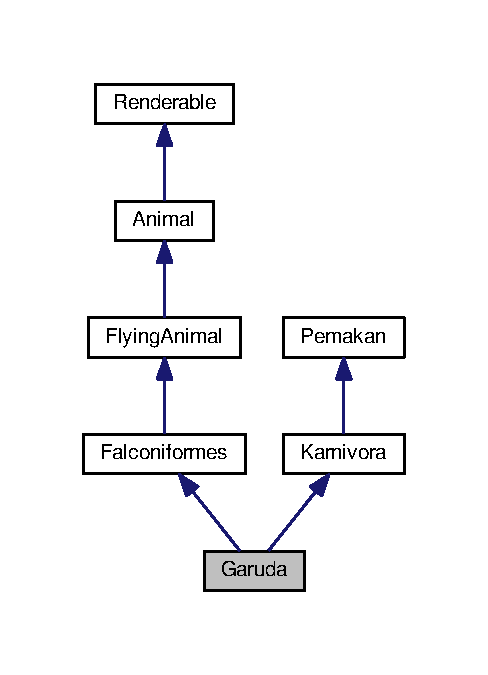
\includegraphics[width=234pt]{classGaruda__inherit__graph}
\end{center}
\end{figure}


Collaboration diagram for Garuda\+:
\nopagebreak
\begin{figure}[H]
\begin{center}
\leavevmode
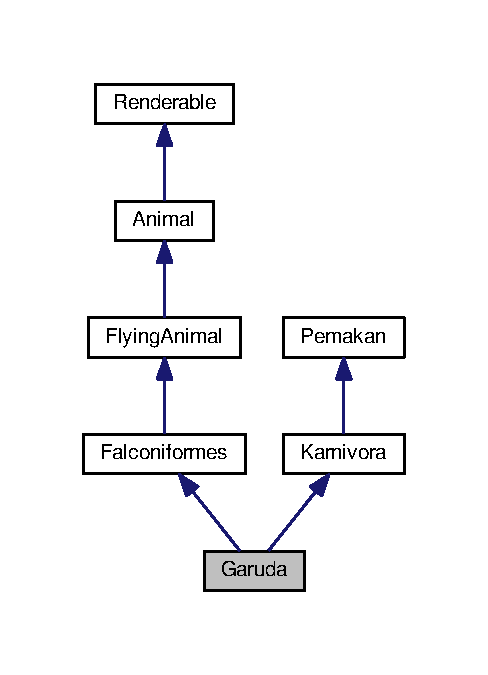
\includegraphics[width=234pt]{classGaruda__coll__graph}
\end{center}
\end{figure}
\subsection*{Public Member Functions}
\begin{DoxyCompactItemize}
\item 
\hyperlink{classGaruda_ae2c20d77a5f7d0d255f32fd2b71f76ee}{Garuda} (int i, int x, int y, int massa, bool jinak)
\begin{DoxyCompactList}\small\item\em Constructor. Menciptakan \hyperlink{classGaruda}{Garuda} dengan inisial \textquotesingle{}G\textquotesingle{} dan ID i. \end{DoxyCompactList}\item 
void \hyperlink{classGaruda_a16d407fcd0ff9fc879641de679cbc456}{Interact} ()\hypertarget{classGaruda_a16d407fcd0ff9fc879641de679cbc456}{}\label{classGaruda_a16d407fcd0ff9fc879641de679cbc456}

\begin{DoxyCompactList}\small\item\em Menampilkan aksi binatang ke layar. \end{DoxyCompactList}\item 
int \hyperlink{classGaruda_a66653e83dc102c16d2a8c99cad247075}{Get\+Jml\+Makanan} ()
\begin{DoxyCompactList}\small\item\em Melihat jumlah makanan dari binatang. Memanggil fungsi Get\+Amount parent \hyperlink{classKarnivora}{Karnivora}. \end{DoxyCompactList}\end{DoxyCompactItemize}
\subsection*{Additional Inherited Members}


\subsection{Detailed Description}
Kelas \hyperlink{classGaruda}{Garuda} turunan dari \hyperlink{classFalconiformes}{Falconiformes} dan \hyperlink{classKarnivora}{Karnivora} 

\subsection{Constructor \& Destructor Documentation}
\index{Garuda@{Garuda}!Garuda@{Garuda}}
\index{Garuda@{Garuda}!Garuda@{Garuda}}
\subsubsection[{\texorpdfstring{Garuda(int i, int x, int y, int massa, bool jinak)}{Garuda(int i, int x, int y, int massa, bool jinak)}}]{\setlength{\rightskip}{0pt plus 5cm}Garuda\+::\+Garuda (
\begin{DoxyParamCaption}
\item[{int}]{i, }
\item[{int}]{x, }
\item[{int}]{y, }
\item[{int}]{massa, }
\item[{bool}]{jinak}
\end{DoxyParamCaption}
)}\hypertarget{classGaruda_ae2c20d77a5f7d0d255f32fd2b71f76ee}{}\label{classGaruda_ae2c20d77a5f7d0d255f32fd2b71f76ee}


Constructor. Menciptakan \hyperlink{classGaruda}{Garuda} dengan inisial \textquotesingle{}G\textquotesingle{} dan ID i. 


\begin{DoxyParams}{Parameters}
{\em i} & Nilai Id \hyperlink{classAnimal}{Animal} yang diciptakan \\
\hline
{\em x} & Posisi x \hyperlink{classAnimal}{Animal} yang diciptakan \\
\hline
{\em y} & Posisi y \hyperlink{classAnimal}{Animal} yang diciptakan \\
\hline
{\em massa} & berat \hyperlink{classAnimal}{Animal} yang diciptakan \\
\hline
{\em jinak} & nilai jinak \hyperlink{classAnimal}{Animal} yang diciptakan \\
\hline
\end{DoxyParams}


\subsection{Member Function Documentation}
\index{Garuda@{Garuda}!Get\+Jml\+Makanan@{Get\+Jml\+Makanan}}
\index{Get\+Jml\+Makanan@{Get\+Jml\+Makanan}!Garuda@{Garuda}}
\subsubsection[{\texorpdfstring{Get\+Jml\+Makanan()}{GetJmlMakanan()}}]{\setlength{\rightskip}{0pt plus 5cm}int Garuda\+::\+Get\+Jml\+Makanan (
\begin{DoxyParamCaption}
{}
\end{DoxyParamCaption}
)\hspace{0.3cm}{\ttfamily [virtual]}}\hypertarget{classGaruda_a66653e83dc102c16d2a8c99cad247075}{}\label{classGaruda_a66653e83dc102c16d2a8c99cad247075}


Melihat jumlah makanan dari binatang. Memanggil fungsi Get\+Amount parent \hyperlink{classKarnivora}{Karnivora}. 

\begin{DoxyReturn}{Returns}
Jumlah makanan dari binatang. 
\end{DoxyReturn}


Implements \hyperlink{classAnimal_a3f1cced7bac93f7c88a24ec5a0e989fe}{Animal}.



The documentation for this class was generated from the following files\+:\begin{DoxyCompactItemize}
\item 
listanimal.\+h\item 
listanimal.\+cpp\end{DoxyCompactItemize}

\hypertarget{classHabitat}{}\section{Habitat Class Reference}
\label{classHabitat}\index{Habitat@{Habitat}}


{\ttfamily \#include $<$zoo.\+h$>$}



Inheritance diagram for Habitat\+:
\nopagebreak
\begin{figure}[H]
\begin{center}
\leavevmode
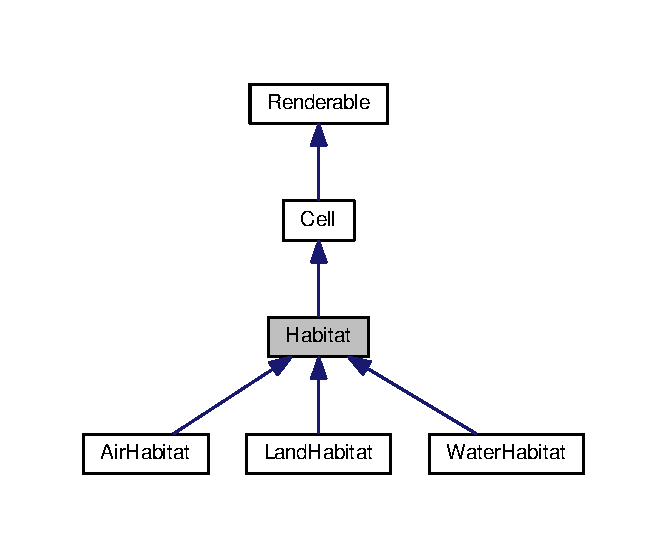
\includegraphics[width=320pt]{classHabitat__inherit__graph}
\end{center}
\end{figure}


Collaboration diagram for Habitat\+:
\nopagebreak
\begin{figure}[H]
\begin{center}
\leavevmode
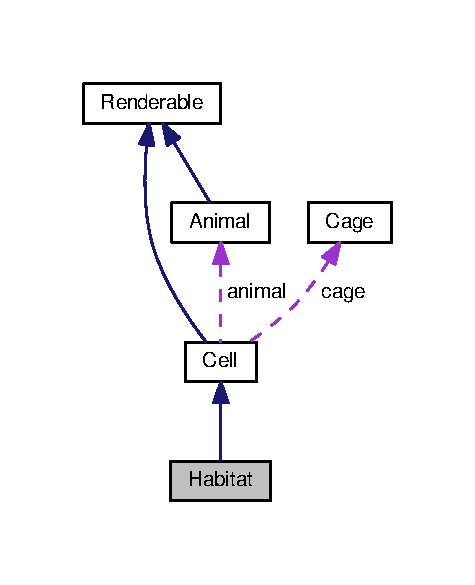
\includegraphics[width=228pt]{classHabitat__coll__graph}
\end{center}
\end{figure}
\subsection*{Public Member Functions}
\begin{DoxyCompactItemize}
\item 
\hyperlink{classHabitat_a86ae5eeab6db20f2bc01095b4454032e}{Habitat} (char c, int x, int y)
\begin{DoxyCompactList}\small\item\em Constructor Menciptakan objek habitat dengan memanggil constructor cell bertype c dan posisi $<$x,y$>$ \end{DoxyCompactList}\item 
void \hyperlink{classHabitat_aa6c8ddf8d46101a9c537bcfd5bd65864}{Render} ()\hypertarget{classHabitat_aa6c8ddf8d46101a9c537bcfd5bd65864}{}\label{classHabitat_aa6c8ddf8d46101a9c537bcfd5bd65864}

\begin{DoxyCompactList}\small\item\em Menampilkan karakter type Jika di habitat terdapat animal maka menampilkan inisial animal ke layar jika tidak menampilkan type ke layar. \end{DoxyCompactList}\end{DoxyCompactItemize}
\subsection*{Additional Inherited Members}


\subsection{Detailed Description}
Kelas \hyperlink{classHabitat}{Habitat} inherit dari kelas \hyperlink{classCell}{Cell}, dapat ditempati oleh hewan 

\subsection{Constructor \& Destructor Documentation}
\index{Habitat@{Habitat}!Habitat@{Habitat}}
\index{Habitat@{Habitat}!Habitat@{Habitat}}
\subsubsection[{\texorpdfstring{Habitat(char c, int x, int y)}{Habitat(char c, int x, int y)}}]{\setlength{\rightskip}{0pt plus 5cm}Habitat\+::\+Habitat (
\begin{DoxyParamCaption}
\item[{char}]{c, }
\item[{int}]{x, }
\item[{int}]{y}
\end{DoxyParamCaption}
)}\hypertarget{classHabitat_a86ae5eeab6db20f2bc01095b4454032e}{}\label{classHabitat_a86ae5eeab6db20f2bc01095b4454032e}


Constructor Menciptakan objek habitat dengan memanggil constructor cell bertype c dan posisi $<$x,y$>$ 


\begin{DoxyParams}{Parameters}
{\em c} & Nilai type habitat yang diciptakan \\
\hline
{\em x} & Nilai absis habitat yang diciptakan \\
\hline
{\em y} & N\+Ilai ordinat habitat yang diciptakan \\
\hline
\end{DoxyParams}


The documentation for this class was generated from the following files\+:\begin{DoxyCompactItemize}
\item 
zoo.\+h\item 
zoo.\+cpp\end{DoxyCompactItemize}

\hypertarget{classHarimauSumatra}{}\section{Harimau\+Sumatra Class Reference}
\label{classHarimauSumatra}\index{Harimau\+Sumatra@{Harimau\+Sumatra}}


{\ttfamily \#include $<$listanimal.\+h$>$}



Inheritance diagram for Harimau\+Sumatra\+:
\nopagebreak
\begin{figure}[H]
\begin{center}
\leavevmode
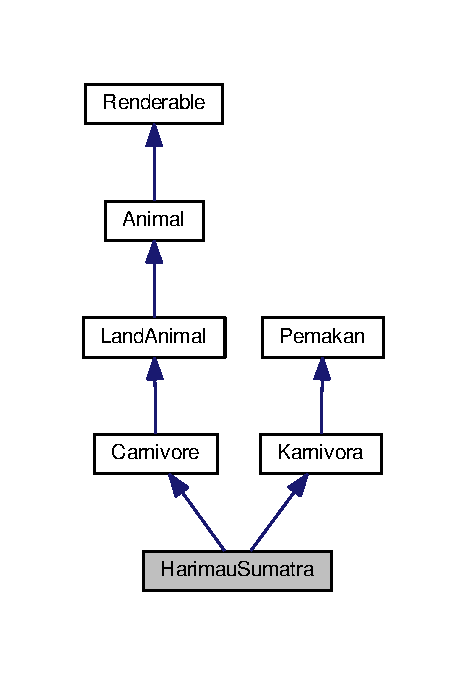
\includegraphics[width=224pt]{classHarimauSumatra__inherit__graph}
\end{center}
\end{figure}


Collaboration diagram for Harimau\+Sumatra\+:
\nopagebreak
\begin{figure}[H]
\begin{center}
\leavevmode
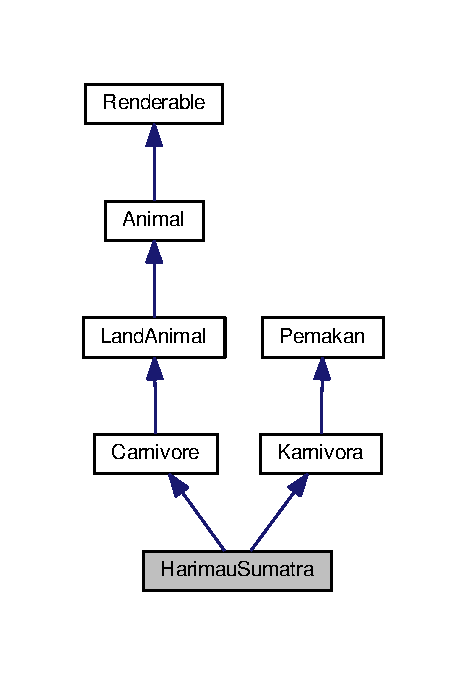
\includegraphics[width=224pt]{classHarimauSumatra__coll__graph}
\end{center}
\end{figure}
\subsection*{Public Member Functions}
\begin{DoxyCompactItemize}
\item 
\hyperlink{classHarimauSumatra_ad2cf7f52161d04f3b8b8d7b78135dba1}{Harimau\+Sumatra} (int i, int x, int y, int massa, bool jinak)
\begin{DoxyCompactList}\small\item\em Constructor. Menciptakan \hyperlink{classHarimauSumatra}{Harimau\+Sumatra} dengan inisial \textquotesingle{}H\textquotesingle{} dan ID i. \end{DoxyCompactList}\item 
void \hyperlink{classHarimauSumatra_a3fdf99e5b76a900085c6cb04a179c90a}{Interact} ()\hypertarget{classHarimauSumatra_a3fdf99e5b76a900085c6cb04a179c90a}{}\label{classHarimauSumatra_a3fdf99e5b76a900085c6cb04a179c90a}

\begin{DoxyCompactList}\small\item\em Menampilkan suara binatang ke layar. \end{DoxyCompactList}\item 
int \hyperlink{classHarimauSumatra_a26c0ee52d2f214027e9998aeef3646e5}{Get\+Jml\+Makanan} ()
\begin{DoxyCompactList}\small\item\em Melihat jumlah makanan dari binatang. Memanggil fungsi Get\+Amount parent \hyperlink{classKarnivora}{Karnivora}. \end{DoxyCompactList}\end{DoxyCompactItemize}
\subsection*{Additional Inherited Members}


\subsection{Detailed Description}
Kelas \hyperlink{classHarimauSumatra}{Harimau\+Sumatra} turunan dari \hyperlink{classCarnivore}{Carnivore} dan \hyperlink{classKarnivora}{Karnivora} 

\subsection{Constructor \& Destructor Documentation}
\index{Harimau\+Sumatra@{Harimau\+Sumatra}!Harimau\+Sumatra@{Harimau\+Sumatra}}
\index{Harimau\+Sumatra@{Harimau\+Sumatra}!Harimau\+Sumatra@{Harimau\+Sumatra}}
\subsubsection[{\texorpdfstring{Harimau\+Sumatra(int i, int x, int y, int massa, bool jinak)}{HarimauSumatra(int i, int x, int y, int massa, bool jinak)}}]{\setlength{\rightskip}{0pt plus 5cm}Harimau\+Sumatra\+::\+Harimau\+Sumatra (
\begin{DoxyParamCaption}
\item[{int}]{i, }
\item[{int}]{x, }
\item[{int}]{y, }
\item[{int}]{massa, }
\item[{bool}]{jinak}
\end{DoxyParamCaption}
)}\hypertarget{classHarimauSumatra_ad2cf7f52161d04f3b8b8d7b78135dba1}{}\label{classHarimauSumatra_ad2cf7f52161d04f3b8b8d7b78135dba1}


Constructor. Menciptakan \hyperlink{classHarimauSumatra}{Harimau\+Sumatra} dengan inisial \textquotesingle{}H\textquotesingle{} dan ID i. 


\begin{DoxyParams}{Parameters}
{\em i} & Nilai Id \hyperlink{classAnimal}{Animal} yang diciptakan \\
\hline
{\em x} & Posisi x \hyperlink{classAnimal}{Animal} yang diciptakan \\
\hline
{\em y} & Posisi y \hyperlink{classAnimal}{Animal} yang diciptakan \\
\hline
{\em massa} & berat \hyperlink{classAnimal}{Animal} yang diciptakan \\
\hline
{\em jinak} & nilai jinak \hyperlink{classAnimal}{Animal} yang diciptakan \\
\hline
\end{DoxyParams}


\subsection{Member Function Documentation}
\index{Harimau\+Sumatra@{Harimau\+Sumatra}!Get\+Jml\+Makanan@{Get\+Jml\+Makanan}}
\index{Get\+Jml\+Makanan@{Get\+Jml\+Makanan}!Harimau\+Sumatra@{Harimau\+Sumatra}}
\subsubsection[{\texorpdfstring{Get\+Jml\+Makanan()}{GetJmlMakanan()}}]{\setlength{\rightskip}{0pt plus 5cm}int Harimau\+Sumatra\+::\+Get\+Jml\+Makanan (
\begin{DoxyParamCaption}
{}
\end{DoxyParamCaption}
)\hspace{0.3cm}{\ttfamily [virtual]}}\hypertarget{classHarimauSumatra_a26c0ee52d2f214027e9998aeef3646e5}{}\label{classHarimauSumatra_a26c0ee52d2f214027e9998aeef3646e5}


Melihat jumlah makanan dari binatang. Memanggil fungsi Get\+Amount parent \hyperlink{classKarnivora}{Karnivora}. 

\begin{DoxyReturn}{Returns}
Jumlah makanan dari binatang. 
\end{DoxyReturn}


Implements \hyperlink{classAnimal_a3f1cced7bac93f7c88a24ec5a0e989fe}{Animal}.



The documentation for this class was generated from the following files\+:\begin{DoxyCompactItemize}
\item 
listanimal.\+h\item 
listanimal.\+cpp\end{DoxyCompactItemize}

\hypertarget{structnlohmann_1_1detail_1_1has__from__json}{}\section{nlohmann\+:\+:detail\+:\+:has\+\_\+from\+\_\+json$<$ Basic\+Json\+Type, T $>$ Struct Template Reference}
\label{structnlohmann_1_1detail_1_1has__from__json}\index{nlohmann\+::detail\+::has\+\_\+from\+\_\+json$<$ Basic\+Json\+Type, T $>$@{nlohmann\+::detail\+::has\+\_\+from\+\_\+json$<$ Basic\+Json\+Type, T $>$}}
\subsection*{Static Public Attributes}
\begin{DoxyCompactItemize}
\item 
static constexpr bool {\bfseries value}
\end{DoxyCompactItemize}


\subsection{Member Data Documentation}
\index{nlohmann\+::detail\+::has\+\_\+from\+\_\+json@{nlohmann\+::detail\+::has\+\_\+from\+\_\+json}!value@{value}}
\index{value@{value}!nlohmann\+::detail\+::has\+\_\+from\+\_\+json@{nlohmann\+::detail\+::has\+\_\+from\+\_\+json}}
\subsubsection[{\texorpdfstring{value}{value}}]{\setlength{\rightskip}{0pt plus 5cm}template$<$typename Basic\+Json\+Type , typename T $>$ constexpr bool {\bf nlohmann\+::detail\+::has\+\_\+from\+\_\+json}$<$ Basic\+Json\+Type, T $>$\+::value\hspace{0.3cm}{\ttfamily [static]}}\hypertarget{structnlohmann_1_1detail_1_1has__from__json_a16701d806343c58ae7e884024dd14955}{}\label{structnlohmann_1_1detail_1_1has__from__json_a16701d806343c58ae7e884024dd14955}
{\bfseries Initial value\+:}
\begin{DoxyCode}
= std::is\_integral<decltype(
                                      detect(std::declval<\textcolor{keyword}{typename} BasicJsonType::template 
      json\_serializer<T, void>>()))>::value
\end{DoxyCode}


The documentation for this struct was generated from the following file\+:\begin{DoxyCompactItemize}
\item 
json.\+hpp\end{DoxyCompactItemize}

\hypertarget{structnlohmann_1_1detail_1_1has__non__default__from__json}{}\section{nlohmann\+:\+:detail\+:\+:has\+\_\+non\+\_\+default\+\_\+from\+\_\+json$<$ Basic\+Json\+Type, T $>$ Struct Template Reference}
\label{structnlohmann_1_1detail_1_1has__non__default__from__json}\index{nlohmann\+::detail\+::has\+\_\+non\+\_\+default\+\_\+from\+\_\+json$<$ Basic\+Json\+Type, T $>$@{nlohmann\+::detail\+::has\+\_\+non\+\_\+default\+\_\+from\+\_\+json$<$ Basic\+Json\+Type, T $>$}}
\subsection*{Static Public Attributes}
\begin{DoxyCompactItemize}
\item 
static constexpr bool {\bfseries value}
\end{DoxyCompactItemize}


\subsection{Member Data Documentation}
\index{nlohmann\+::detail\+::has\+\_\+non\+\_\+default\+\_\+from\+\_\+json@{nlohmann\+::detail\+::has\+\_\+non\+\_\+default\+\_\+from\+\_\+json}!value@{value}}
\index{value@{value}!nlohmann\+::detail\+::has\+\_\+non\+\_\+default\+\_\+from\+\_\+json@{nlohmann\+::detail\+::has\+\_\+non\+\_\+default\+\_\+from\+\_\+json}}
\subsubsection[{\texorpdfstring{value}{value}}]{\setlength{\rightskip}{0pt plus 5cm}template$<$typename Basic\+Json\+Type , typename T $>$ constexpr bool {\bf nlohmann\+::detail\+::has\+\_\+non\+\_\+default\+\_\+from\+\_\+json}$<$ Basic\+Json\+Type, T $>$\+::value\hspace{0.3cm}{\ttfamily [static]}}\hypertarget{structnlohmann_1_1detail_1_1has__non__default__from__json_ad34bb7cd3961fcafc2c5047a9782e931}{}\label{structnlohmann_1_1detail_1_1has__non__default__from__json_ad34bb7cd3961fcafc2c5047a9782e931}
{\bfseries Initial value\+:}
\begin{DoxyCode}
= std::is\_integral<decltype(detect(
                                      std::declval<\textcolor{keyword}{typename} BasicJsonType::template json\_serializer<T,
       void>>()))>::value
\end{DoxyCode}


The documentation for this struct was generated from the following file\+:\begin{DoxyCompactItemize}
\item 
json.\+hpp\end{DoxyCompactItemize}

\hypertarget{structnlohmann_1_1detail_1_1has__to__json}{}\section{nlohmann\+:\+:detail\+:\+:has\+\_\+to\+\_\+json$<$ Basic\+Json\+Type, T $>$ Struct Template Reference}
\label{structnlohmann_1_1detail_1_1has__to__json}\index{nlohmann\+::detail\+::has\+\_\+to\+\_\+json$<$ Basic\+Json\+Type, T $>$@{nlohmann\+::detail\+::has\+\_\+to\+\_\+json$<$ Basic\+Json\+Type, T $>$}}
\subsection*{Static Public Attributes}
\begin{DoxyCompactItemize}
\item 
static constexpr bool {\bfseries value}
\end{DoxyCompactItemize}


\subsection{Member Data Documentation}
\index{nlohmann\+::detail\+::has\+\_\+to\+\_\+json@{nlohmann\+::detail\+::has\+\_\+to\+\_\+json}!value@{value}}
\index{value@{value}!nlohmann\+::detail\+::has\+\_\+to\+\_\+json@{nlohmann\+::detail\+::has\+\_\+to\+\_\+json}}
\subsubsection[{\texorpdfstring{value}{value}}]{\setlength{\rightskip}{0pt plus 5cm}template$<$typename Basic\+Json\+Type , typename T $>$ constexpr bool {\bf nlohmann\+::detail\+::has\+\_\+to\+\_\+json}$<$ Basic\+Json\+Type, T $>$\+::value\hspace{0.3cm}{\ttfamily [static]}}\hypertarget{structnlohmann_1_1detail_1_1has__to__json_a18e260c3c6f10328637c4427d3cb3a31}{}\label{structnlohmann_1_1detail_1_1has__to__json_a18e260c3c6f10328637c4427d3cb3a31}
{\bfseries Initial value\+:}
\begin{DoxyCode}
= std::is\_integral<decltype(detect(
                                      std::declval<\textcolor{keyword}{typename} BasicJsonType::template json\_serializer<T,
       void>>()))>::value
\end{DoxyCode}


The documentation for this struct was generated from the following file\+:\begin{DoxyCompactItemize}
\item 
json.\+hpp\end{DoxyCompactItemize}

\hypertarget{structstd_1_1hash_3_01nlohmann_1_1json_01_4}{}\section{std\+:\+:hash$<$ nlohmann\+:\+:json $>$ Struct Template Reference}
\label{structstd_1_1hash_3_01nlohmann_1_1json_01_4}\index{std\+::hash$<$ nlohmann\+::json $>$@{std\+::hash$<$ nlohmann\+::json $>$}}


hash value for J\+S\+ON objects  




{\ttfamily \#include $<$json.\+hpp$>$}

\subsection*{Public Member Functions}
\begin{DoxyCompactItemize}
\item 
std\+::size\+\_\+t \hyperlink{structstd_1_1hash_3_01nlohmann_1_1json_01_4_afd03f6ad53db22868ca4163a8200b2f9}{operator()} (const \hyperlink{namespacenlohmann_a2bfd99e845a2e5cd90aeaf1b1431f474}{nlohmann\+::json} \&j) const 
\begin{DoxyCompactList}\small\item\em return a hash value for a J\+S\+ON object \end{DoxyCompactList}\end{DoxyCompactItemize}


\subsection{Detailed Description}
\subsubsection*{template$<$$>$\\*
struct std\+::hash$<$ nlohmann\+::json $>$}

hash value for J\+S\+ON objects 

\subsection{Member Function Documentation}
\index{std\+::hash$<$ nlohmann\+::json $>$@{std\+::hash$<$ nlohmann\+::json $>$}!operator()@{operator()}}
\index{operator()@{operator()}!std\+::hash$<$ nlohmann\+::json $>$@{std\+::hash$<$ nlohmann\+::json $>$}}
\subsubsection[{\texorpdfstring{operator()(const nlohmann\+::json \&j) const }{operator()(const nlohmann::json &j) const }}]{\setlength{\rightskip}{0pt plus 5cm}std\+::size\+\_\+t std\+::hash$<$ {\bf nlohmann\+::json} $>$\+::operator() (
\begin{DoxyParamCaption}
\item[{const {\bf nlohmann\+::json} \&}]{j}
\end{DoxyParamCaption}
) const\hspace{0.3cm}{\ttfamily [inline]}}\hypertarget{structstd_1_1hash_3_01nlohmann_1_1json_01_4_afd03f6ad53db22868ca4163a8200b2f9}{}\label{structstd_1_1hash_3_01nlohmann_1_1json_01_4_afd03f6ad53db22868ca4163a8200b2f9}


return a hash value for a J\+S\+ON object 

\begin{DoxySince}{Since}
version 1.\+0.\+0 
\end{DoxySince}


The documentation for this struct was generated from the following file\+:\begin{DoxyCompactItemize}
\item 
json.\+hpp\end{DoxyCompactItemize}

\hypertarget{classHerbivora}{}\section{Herbivora Class Reference}
\label{classHerbivora}\index{Herbivora@{Herbivora}}


{\ttfamily \#include $<$pemakan.\+h$>$}



Inheritance diagram for Herbivora\+:
\nopagebreak
\begin{figure}[H]
\begin{center}
\leavevmode
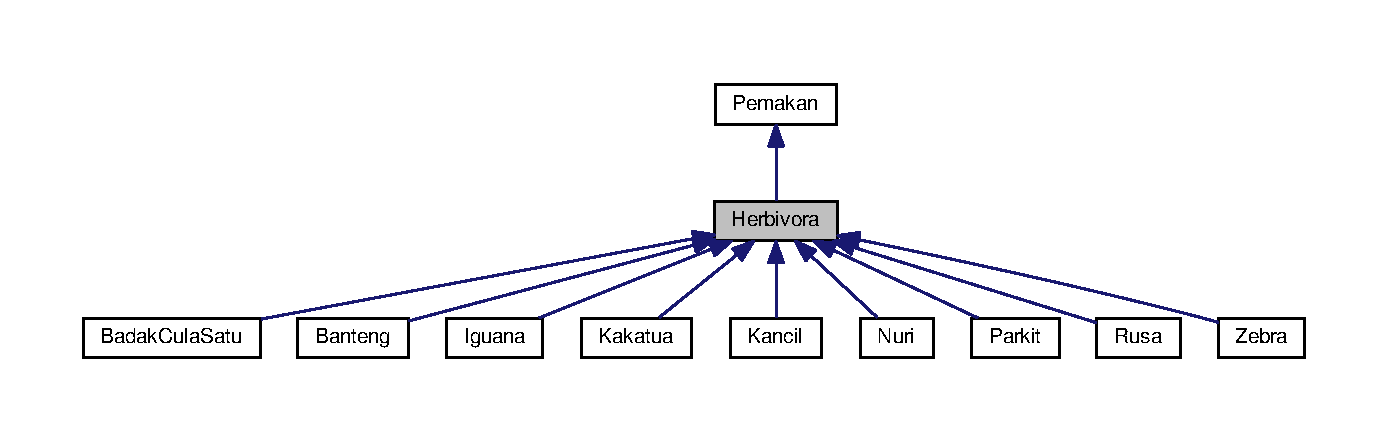
\includegraphics[width=350pt]{classHerbivora__inherit__graph}
\end{center}
\end{figure}


Collaboration diagram for Herbivora\+:
\nopagebreak
\begin{figure}[H]
\begin{center}
\leavevmode
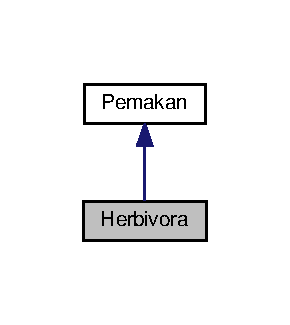
\includegraphics[width=139pt]{classHerbivora__coll__graph}
\end{center}
\end{figure}
\subsection*{Public Member Functions}
\begin{DoxyCompactItemize}
\item 
void \hyperlink{classHerbivora_a271d3947a772bee2ab3512c09cea2fe9}{Set\+Amount} (int n)
\begin{DoxyCompactList}\small\item\em Setter tumbuhan. \end{DoxyCompactList}\item 
int \hyperlink{classHerbivora_a2533747fe5eb914c9731e83655af457e}{Get\+Amount} ()
\begin{DoxyCompactList}\small\item\em Getter tumbuhan. \end{DoxyCompactList}\end{DoxyCompactItemize}
\subsection*{Protected Attributes}
\begin{DoxyCompactItemize}
\item 
int {\bfseries tumbuhan}\hypertarget{classHerbivora_ae77c85f52d5fb5b2474e92d00d4a84fa}{}\label{classHerbivora_ae77c85f52d5fb5b2474e92d00d4a84fa}

\end{DoxyCompactItemize}


\subsection{Detailed Description}
Kelas \hyperlink{classHerbivora}{Herbivora} menyimpan informasi makanan berupa tumbuhan 

\subsection{Member Function Documentation}
\index{Herbivora@{Herbivora}!Get\+Amount@{Get\+Amount}}
\index{Get\+Amount@{Get\+Amount}!Herbivora@{Herbivora}}
\subsubsection[{\texorpdfstring{Get\+Amount()}{GetAmount()}}]{\setlength{\rightskip}{0pt plus 5cm}int Herbivora\+::\+Get\+Amount (
\begin{DoxyParamCaption}
{}
\end{DoxyParamCaption}
)\hspace{0.3cm}{\ttfamily [virtual]}}\hypertarget{classHerbivora_a2533747fe5eb914c9731e83655af457e}{}\label{classHerbivora_a2533747fe5eb914c9731e83655af457e}


Getter tumbuhan. 

\begin{DoxyReturn}{Returns}
tumbuhan 
\end{DoxyReturn}


Implements \hyperlink{classPemakan_a7b955f34ce9bfda6cf41d4e89b2f729d}{Pemakan}.

\index{Herbivora@{Herbivora}!Set\+Amount@{Set\+Amount}}
\index{Set\+Amount@{Set\+Amount}!Herbivora@{Herbivora}}
\subsubsection[{\texorpdfstring{Set\+Amount(int n)}{SetAmount(int n)}}]{\setlength{\rightskip}{0pt plus 5cm}void Herbivora\+::\+Set\+Amount (
\begin{DoxyParamCaption}
\item[{int}]{n}
\end{DoxyParamCaption}
)}\hypertarget{classHerbivora_a271d3947a772bee2ab3512c09cea2fe9}{}\label{classHerbivora_a271d3947a772bee2ab3512c09cea2fe9}


Setter tumbuhan. 


\begin{DoxyParams}{Parameters}
{\em n} & Jumlah tumbuhan yang diinginkan \\
\hline
\end{DoxyParams}


The documentation for this class was generated from the following files\+:\begin{DoxyCompactItemize}
\item 
pemakan.\+h\item 
pemakan.\+cpp\end{DoxyCompactItemize}

\hypertarget{classHiuKarpet}{}\section{Hiu\+Karpet Class Reference}
\label{classHiuKarpet}\index{Hiu\+Karpet@{Hiu\+Karpet}}


{\ttfamily \#include $<$listanimal.\+h$>$}



Inheritance diagram for Hiu\+Karpet\+:
\nopagebreak
\begin{figure}[H]
\begin{center}
\leavevmode
\includegraphics[width=252pt]{classHiuKarpet__inherit__graph}
\end{center}
\end{figure}


Collaboration diagram for Hiu\+Karpet\+:
\nopagebreak
\begin{figure}[H]
\begin{center}
\leavevmode
\includegraphics[width=252pt]{classHiuKarpet__coll__graph}
\end{center}
\end{figure}
\subsection*{Public Member Functions}
\begin{DoxyCompactItemize}
\item 
\hyperlink{classHiuKarpet_ac1589c25b08eb4b0d33deec9e5dcabc5}{Hiu\+Karpet} (int i, int x, int y, int massa, bool jinak)
\begin{DoxyCompactList}\small\item\em Constructor. Menciptakan \hyperlink{classHiuKarpet}{Hiu\+Karpet} dengan inisial \textquotesingle{}V\textquotesingle{} dan ID i. \end{DoxyCompactList}\item 
void \hyperlink{classHiuKarpet_a5aecaaf80c31e829c06abb3f90ad47da}{Interact} ()\hypertarget{classHiuKarpet_a5aecaaf80c31e829c06abb3f90ad47da}{}\label{classHiuKarpet_a5aecaaf80c31e829c06abb3f90ad47da}

\begin{DoxyCompactList}\small\item\em Menampilkan aksi binatang ke layar. \end{DoxyCompactList}\item 
int \hyperlink{classHiuKarpet_abcb51ba250304ab5b9a0a649c1e705d1}{Get\+Jml\+Makanan} ()
\begin{DoxyCompactList}\small\item\em Melihat jumlah makanan dari binatang. Memanggil fungsi Get\+Amount parent \hyperlink{classKarnivora}{Karnivora}. \end{DoxyCompactList}\end{DoxyCompactItemize}
\subsection*{Additional Inherited Members}


\subsection{Detailed Description}
Kelas \hyperlink{classHiuKarpet}{Hiu\+Karpet} turunan dari \hyperlink{classCarcharhiniformes}{Carcharhiniformes} dan \hyperlink{classKarnivora}{Karnivora} 

\subsection{Constructor \& Destructor Documentation}
\index{Hiu\+Karpet@{Hiu\+Karpet}!Hiu\+Karpet@{Hiu\+Karpet}}
\index{Hiu\+Karpet@{Hiu\+Karpet}!Hiu\+Karpet@{Hiu\+Karpet}}
\subsubsection[{\texorpdfstring{Hiu\+Karpet(int i, int x, int y, int massa, bool jinak)}{HiuKarpet(int i, int x, int y, int massa, bool jinak)}}]{\setlength{\rightskip}{0pt plus 5cm}Hiu\+Karpet\+::\+Hiu\+Karpet (
\begin{DoxyParamCaption}
\item[{int}]{i, }
\item[{int}]{x, }
\item[{int}]{y, }
\item[{int}]{massa, }
\item[{bool}]{jinak}
\end{DoxyParamCaption}
)}\hypertarget{classHiuKarpet_ac1589c25b08eb4b0d33deec9e5dcabc5}{}\label{classHiuKarpet_ac1589c25b08eb4b0d33deec9e5dcabc5}


Constructor. Menciptakan \hyperlink{classHiuKarpet}{Hiu\+Karpet} dengan inisial \textquotesingle{}V\textquotesingle{} dan ID i. 


\begin{DoxyParams}{Parameters}
{\em i} & Nilai Id \hyperlink{classAnimal}{Animal} yang diciptakan \\
\hline
{\em x} & Posisi x \hyperlink{classAnimal}{Animal} yang diciptakan \\
\hline
{\em y} & Posisi y \hyperlink{classAnimal}{Animal} yang diciptakan \\
\hline
{\em massa} & berat \hyperlink{classAnimal}{Animal} yang diciptakan \\
\hline
{\em jinak} & nilai jinak \hyperlink{classAnimal}{Animal} yang diciptakan \\
\hline
\end{DoxyParams}


\subsection{Member Function Documentation}
\index{Hiu\+Karpet@{Hiu\+Karpet}!Get\+Jml\+Makanan@{Get\+Jml\+Makanan}}
\index{Get\+Jml\+Makanan@{Get\+Jml\+Makanan}!Hiu\+Karpet@{Hiu\+Karpet}}
\subsubsection[{\texorpdfstring{Get\+Jml\+Makanan()}{GetJmlMakanan()}}]{\setlength{\rightskip}{0pt plus 5cm}int Hiu\+Karpet\+::\+Get\+Jml\+Makanan (
\begin{DoxyParamCaption}
{}
\end{DoxyParamCaption}
)\hspace{0.3cm}{\ttfamily [virtual]}}\hypertarget{classHiuKarpet_abcb51ba250304ab5b9a0a649c1e705d1}{}\label{classHiuKarpet_abcb51ba250304ab5b9a0a649c1e705d1}


Melihat jumlah makanan dari binatang. Memanggil fungsi Get\+Amount parent \hyperlink{classKarnivora}{Karnivora}. 

\begin{DoxyReturn}{Returns}
Jumlah makanan dari binatang. 
\end{DoxyReturn}


Implements \hyperlink{classAnimal_a3f1cced7bac93f7c88a24ec5a0e989fe}{Animal}.



The documentation for this class was generated from the following files\+:\begin{DoxyCompactItemize}
\item 
listanimal.\+h\item 
listanimal.\+cpp\end{DoxyCompactItemize}

\hypertarget{classHiuMartil}{}\section{Hiu\+Martil Class Reference}
\label{classHiuMartil}\index{Hiu\+Martil@{Hiu\+Martil}}


{\ttfamily \#include $<$listanimal.\+h$>$}



Inheritance diagram for Hiu\+Martil\+:
\nopagebreak
\begin{figure}[H]
\begin{center}
\leavevmode
\includegraphics[width=252pt]{classHiuMartil__inherit__graph}
\end{center}
\end{figure}


Collaboration diagram for Hiu\+Martil\+:
\nopagebreak
\begin{figure}[H]
\begin{center}
\leavevmode
\includegraphics[width=252pt]{classHiuMartil__coll__graph}
\end{center}
\end{figure}
\subsection*{Public Member Functions}
\begin{DoxyCompactItemize}
\item 
\hyperlink{classHiuMartil_a376ac60795c3c37cec40714635d47b8a}{Hiu\+Martil} (int i, int x, int y, int massa, bool jinak)
\begin{DoxyCompactList}\small\item\em Constructor. Menciptakan \hyperlink{classHiuMartil}{Hiu\+Martil} dengan inisial \textquotesingle{}T\textquotesingle{} dan ID i. \end{DoxyCompactList}\item 
void \hyperlink{classHiuMartil_a9329d5115ecdfd2eb91137b481dfe863}{Interact} ()\hypertarget{classHiuMartil_a9329d5115ecdfd2eb91137b481dfe863}{}\label{classHiuMartil_a9329d5115ecdfd2eb91137b481dfe863}

\begin{DoxyCompactList}\small\item\em Menampilkan aksi binatang ke layar. \end{DoxyCompactList}\item 
int \hyperlink{classHiuMartil_a8b643c318a9b69730c26a73b268f0b2c}{Get\+Jml\+Makanan} ()
\begin{DoxyCompactList}\small\item\em Melihat jumlah makanan dari binatang. Memanggil fungsi Get\+Amount parent Karivora. \end{DoxyCompactList}\end{DoxyCompactItemize}
\subsection*{Additional Inherited Members}


\subsection{Detailed Description}
Kelas \hyperlink{classHiuMartil}{Hiu\+Martil} turunan dari \hyperlink{classCarcharhiniformes}{Carcharhiniformes} dan \hyperlink{classKarnivora}{Karnivora} 

\subsection{Constructor \& Destructor Documentation}
\index{Hiu\+Martil@{Hiu\+Martil}!Hiu\+Martil@{Hiu\+Martil}}
\index{Hiu\+Martil@{Hiu\+Martil}!Hiu\+Martil@{Hiu\+Martil}}
\subsubsection[{\texorpdfstring{Hiu\+Martil(int i, int x, int y, int massa, bool jinak)}{HiuMartil(int i, int x, int y, int massa, bool jinak)}}]{\setlength{\rightskip}{0pt plus 5cm}Hiu\+Martil\+::\+Hiu\+Martil (
\begin{DoxyParamCaption}
\item[{int}]{i, }
\item[{int}]{x, }
\item[{int}]{y, }
\item[{int}]{massa, }
\item[{bool}]{jinak}
\end{DoxyParamCaption}
)}\hypertarget{classHiuMartil_a376ac60795c3c37cec40714635d47b8a}{}\label{classHiuMartil_a376ac60795c3c37cec40714635d47b8a}


Constructor. Menciptakan \hyperlink{classHiuMartil}{Hiu\+Martil} dengan inisial \textquotesingle{}T\textquotesingle{} dan ID i. 


\begin{DoxyParams}{Parameters}
{\em i} & Nilai Id \hyperlink{classAnimal}{Animal} yang diciptakan \\
\hline
{\em x} & Posisi x \hyperlink{classAnimal}{Animal} yang diciptakan \\
\hline
{\em y} & Posisi y \hyperlink{classAnimal}{Animal} yang diciptakan \\
\hline
{\em massa} & berat \hyperlink{classAnimal}{Animal} yang diciptakan \\
\hline
{\em jinak} & nilai jinak \hyperlink{classAnimal}{Animal} yang diciptakan \\
\hline
\end{DoxyParams}


\subsection{Member Function Documentation}
\index{Hiu\+Martil@{Hiu\+Martil}!Get\+Jml\+Makanan@{Get\+Jml\+Makanan}}
\index{Get\+Jml\+Makanan@{Get\+Jml\+Makanan}!Hiu\+Martil@{Hiu\+Martil}}
\subsubsection[{\texorpdfstring{Get\+Jml\+Makanan()}{GetJmlMakanan()}}]{\setlength{\rightskip}{0pt plus 5cm}int Hiu\+Martil\+::\+Get\+Jml\+Makanan (
\begin{DoxyParamCaption}
{}
\end{DoxyParamCaption}
)\hspace{0.3cm}{\ttfamily [virtual]}}\hypertarget{classHiuMartil_a8b643c318a9b69730c26a73b268f0b2c}{}\label{classHiuMartil_a8b643c318a9b69730c26a73b268f0b2c}


Melihat jumlah makanan dari binatang. Memanggil fungsi Get\+Amount parent Karivora. 

\begin{DoxyReturn}{Returns}
Jumlah makanan dari binatang. 
\end{DoxyReturn}


Implements \hyperlink{classAnimal_a3f1cced7bac93f7c88a24ec5a0e989fe}{Animal}.



The documentation for this class was generated from the following files\+:\begin{DoxyCompactItemize}
\item 
listanimal.\+h\item 
listanimal.\+cpp\end{DoxyCompactItemize}

\hypertarget{classIguana}{}\section{Iguana Class Reference}
\label{classIguana}\index{Iguana@{Iguana}}


{\ttfamily \#include $<$listanimal.\+h$>$}



Inheritance diagram for Iguana\+:
\nopagebreak
\begin{figure}[H]
\begin{center}
\leavevmode
\includegraphics[width=224pt]{classIguana__inherit__graph}
\end{center}
\end{figure}


Collaboration diagram for Iguana\+:
\nopagebreak
\begin{figure}[H]
\begin{center}
\leavevmode
\includegraphics[width=224pt]{classIguana__coll__graph}
\end{center}
\end{figure}
\subsection*{Public Member Functions}
\begin{DoxyCompactItemize}
\item 
\hyperlink{classIguana_a36cea5dad12ace3182deab6fd7ab1b25}{Iguana} (int i, int x, int y, int massa, bool jinak)
\begin{DoxyCompactList}\small\item\em Constructor. Menciptakan \hyperlink{classIguana}{Iguana} dengan inisial \textquotesingle{}I\textquotesingle{} dan ID i. \end{DoxyCompactList}\item 
void \hyperlink{classIguana_aba316410fc6fc8b81bfbde17a733dd0e}{Interact} ()\hypertarget{classIguana_aba316410fc6fc8b81bfbde17a733dd0e}{}\label{classIguana_aba316410fc6fc8b81bfbde17a733dd0e}

\begin{DoxyCompactList}\small\item\em Menampilkan suara binatang ke layar. \end{DoxyCompactList}\item 
int \hyperlink{classIguana_ae871a38dfe31ebba979268ba881cff1a}{Get\+Jml\+Makanan} ()
\begin{DoxyCompactList}\small\item\em Melihat jumlah makanan dari binatang. Memanggil fungsi Get\+Amount parent \hyperlink{classHerbivora}{Herbivora}. \end{DoxyCompactList}\end{DoxyCompactItemize}
\subsection*{Additional Inherited Members}


\subsection{Detailed Description}
Kelas \hyperlink{classIguana}{Iguana} turunan dari \hyperlink{classSquamata}{Squamata} dan \hyperlink{classHerbivora}{Herbivora} 

\subsection{Constructor \& Destructor Documentation}
\index{Iguana@{Iguana}!Iguana@{Iguana}}
\index{Iguana@{Iguana}!Iguana@{Iguana}}
\subsubsection[{\texorpdfstring{Iguana(int i, int x, int y, int massa, bool jinak)}{Iguana(int i, int x, int y, int massa, bool jinak)}}]{\setlength{\rightskip}{0pt plus 5cm}Iguana\+::\+Iguana (
\begin{DoxyParamCaption}
\item[{int}]{i, }
\item[{int}]{x, }
\item[{int}]{y, }
\item[{int}]{massa, }
\item[{bool}]{jinak}
\end{DoxyParamCaption}
)}\hypertarget{classIguana_a36cea5dad12ace3182deab6fd7ab1b25}{}\label{classIguana_a36cea5dad12ace3182deab6fd7ab1b25}


Constructor. Menciptakan \hyperlink{classIguana}{Iguana} dengan inisial \textquotesingle{}I\textquotesingle{} dan ID i. 


\begin{DoxyParams}{Parameters}
{\em i} & Nilai Id \hyperlink{classAnimal}{Animal} yang diciptakan \\
\hline
{\em x} & Posisi x \hyperlink{classAnimal}{Animal} yang diciptakan \\
\hline
{\em y} & Posisi y \hyperlink{classAnimal}{Animal} yang diciptakan \\
\hline
{\em massa} & berat \hyperlink{classAnimal}{Animal} yang diciptakan \\
\hline
{\em jinak} & nilai jinak \hyperlink{classAnimal}{Animal} yang diciptakan \\
\hline
\end{DoxyParams}


\subsection{Member Function Documentation}
\index{Iguana@{Iguana}!Get\+Jml\+Makanan@{Get\+Jml\+Makanan}}
\index{Get\+Jml\+Makanan@{Get\+Jml\+Makanan}!Iguana@{Iguana}}
\subsubsection[{\texorpdfstring{Get\+Jml\+Makanan()}{GetJmlMakanan()}}]{\setlength{\rightskip}{0pt plus 5cm}int Iguana\+::\+Get\+Jml\+Makanan (
\begin{DoxyParamCaption}
{}
\end{DoxyParamCaption}
)\hspace{0.3cm}{\ttfamily [virtual]}}\hypertarget{classIguana_ae871a38dfe31ebba979268ba881cff1a}{}\label{classIguana_ae871a38dfe31ebba979268ba881cff1a}


Melihat jumlah makanan dari binatang. Memanggil fungsi Get\+Amount parent \hyperlink{classHerbivora}{Herbivora}. 

\begin{DoxyReturn}{Returns}
Jumlah makanan dari binatang. 
\end{DoxyReturn}


Implements \hyperlink{classAnimal_a3f1cced7bac93f7c88a24ec5a0e989fe}{Animal}.



The documentation for this class was generated from the following files\+:\begin{DoxyCompactItemize}
\item 
listanimal.\+h\item 
listanimal.\+cpp\end{DoxyCompactItemize}

\hypertarget{structnlohmann_1_1detail_1_1is__basic__json__nested__type}{}\section{nlohmann\+:\+:detail\+:\+:is\+\_\+basic\+\_\+json\+\_\+nested\+\_\+type$<$ Basic\+Json\+Type, T $>$ Struct Template Reference}
\label{structnlohmann_1_1detail_1_1is__basic__json__nested__type}\index{nlohmann\+::detail\+::is\+\_\+basic\+\_\+json\+\_\+nested\+\_\+type$<$ Basic\+Json\+Type, T $>$@{nlohmann\+::detail\+::is\+\_\+basic\+\_\+json\+\_\+nested\+\_\+type$<$ Basic\+Json\+Type, T $>$}}
\subsection*{Static Public Attributes}
\begin{DoxyCompactItemize}
\item 
static auto constexpr {\bfseries value}
\end{DoxyCompactItemize}


\subsection{Member Data Documentation}
\index{nlohmann\+::detail\+::is\+\_\+basic\+\_\+json\+\_\+nested\+\_\+type@{nlohmann\+::detail\+::is\+\_\+basic\+\_\+json\+\_\+nested\+\_\+type}!value@{value}}
\index{value@{value}!nlohmann\+::detail\+::is\+\_\+basic\+\_\+json\+\_\+nested\+\_\+type@{nlohmann\+::detail\+::is\+\_\+basic\+\_\+json\+\_\+nested\+\_\+type}}
\subsubsection[{\texorpdfstring{value}{value}}]{\setlength{\rightskip}{0pt plus 5cm}template$<$typename Basic\+Json\+Type , typename T $>$ auto constexpr {\bf nlohmann\+::detail\+::is\+\_\+basic\+\_\+json\+\_\+nested\+\_\+type}$<$ Basic\+Json\+Type, T $>$\+::value\hspace{0.3cm}{\ttfamily [static]}}\hypertarget{structnlohmann_1_1detail_1_1is__basic__json__nested__type_aee5fee744e5298a78d557f2ee5f090db}{}\label{structnlohmann_1_1detail_1_1is__basic__json__nested__type_aee5fee744e5298a78d557f2ee5f090db}
{\bfseries Initial value\+:}
\begin{DoxyCode}
= std::is\_same<T, typename BasicJsonType::iterator>::value or
                                  std::is\_same<T, typename BasicJsonType::const\_iterator>::value or
                                  std::is\_same<T, typename BasicJsonType::reverse\_iterator>::value or
                                  std::is\_same<T, typename BasicJsonType::const\_reverse\_iterator>::value or
                                  std::is\_same<T, typename BasicJsonType::json\_pointer>::value
\end{DoxyCode}


The documentation for this struct was generated from the following file\+:\begin{DoxyCompactItemize}
\item 
json.\+hpp\end{DoxyCompactItemize}

\hypertarget{structnlohmann_1_1detail_1_1is__compatible__array__type}{}\section{nlohmann\+:\+:detail\+:\+:is\+\_\+compatible\+\_\+array\+\_\+type$<$ Basic\+Json\+Type, Compatible\+Array\+Type $>$ Struct Template Reference}
\label{structnlohmann_1_1detail_1_1is__compatible__array__type}\index{nlohmann\+::detail\+::is\+\_\+compatible\+\_\+array\+\_\+type$<$ Basic\+Json\+Type, Compatible\+Array\+Type $>$@{nlohmann\+::detail\+::is\+\_\+compatible\+\_\+array\+\_\+type$<$ Basic\+Json\+Type, Compatible\+Array\+Type $>$}}
\subsection*{Static Public Attributes}
\begin{DoxyCompactItemize}
\item 
static auto constexpr {\bfseries value}
\end{DoxyCompactItemize}


\subsection{Member Data Documentation}
\index{nlohmann\+::detail\+::is\+\_\+compatible\+\_\+array\+\_\+type@{nlohmann\+::detail\+::is\+\_\+compatible\+\_\+array\+\_\+type}!value@{value}}
\index{value@{value}!nlohmann\+::detail\+::is\+\_\+compatible\+\_\+array\+\_\+type@{nlohmann\+::detail\+::is\+\_\+compatible\+\_\+array\+\_\+type}}
\subsubsection[{\texorpdfstring{value}{value}}]{\setlength{\rightskip}{0pt plus 5cm}template$<$class Basic\+Json\+Type , class Compatible\+Array\+Type $>$ auto constexpr {\bf nlohmann\+::detail\+::is\+\_\+compatible\+\_\+array\+\_\+type}$<$ Basic\+Json\+Type, Compatible\+Array\+Type $>$\+::value\hspace{0.3cm}{\ttfamily [static]}}\hypertarget{structnlohmann_1_1detail_1_1is__compatible__array__type_a01bc2274c22746bbb2cefd2acee8b572}{}\label{structnlohmann_1_1detail_1_1is__compatible__array__type_a01bc2274c22746bbb2cefd2acee8b572}
{\bfseries Initial value\+:}
\begin{DoxyCode}
=
        conjunction<negation<std::is\_same<void, CompatibleArrayType>>,
        negation<is\_compatible\_object\_type<
        BasicJsonType, CompatibleArrayType>>,
        negation<std::is\_constructible<\textcolor{keyword}{typename} BasicJsonType::string\_t,
        CompatibleArrayType>>,
        negation<is\_basic\_json\_nested\_type<BasicJsonType, CompatibleArrayType>>,
        has\_value\_type<CompatibleArrayType>,
        has\_iterator<CompatibleArrayType>>::value
\end{DoxyCode}


The documentation for this struct was generated from the following file\+:\begin{DoxyCompactItemize}
\item 
json.\+hpp\end{DoxyCompactItemize}

\hypertarget{structnlohmann_1_1detail_1_1is__compatible__integer__type}{}\section{nlohmann\+:\+:detail\+:\+:is\+\_\+compatible\+\_\+integer\+\_\+type$<$ Real\+Integer\+Type, Compatible\+Number\+Integer\+Type $>$ Struct Template Reference}
\label{structnlohmann_1_1detail_1_1is__compatible__integer__type}\index{nlohmann\+::detail\+::is\+\_\+compatible\+\_\+integer\+\_\+type$<$ Real\+Integer\+Type, Compatible\+Number\+Integer\+Type $>$@{nlohmann\+::detail\+::is\+\_\+compatible\+\_\+integer\+\_\+type$<$ Real\+Integer\+Type, Compatible\+Number\+Integer\+Type $>$}}
\subsection*{Static Public Attributes}
\begin{DoxyCompactItemize}
\item 
static constexpr auto {\bfseries value}
\end{DoxyCompactItemize}


\subsection{Member Data Documentation}
\index{nlohmann\+::detail\+::is\+\_\+compatible\+\_\+integer\+\_\+type@{nlohmann\+::detail\+::is\+\_\+compatible\+\_\+integer\+\_\+type}!value@{value}}
\index{value@{value}!nlohmann\+::detail\+::is\+\_\+compatible\+\_\+integer\+\_\+type@{nlohmann\+::detail\+::is\+\_\+compatible\+\_\+integer\+\_\+type}}
\subsubsection[{\texorpdfstring{value}{value}}]{\setlength{\rightskip}{0pt plus 5cm}template$<$typename Real\+Integer\+Type , typename Compatible\+Number\+Integer\+Type $>$ constexpr auto {\bf nlohmann\+::detail\+::is\+\_\+compatible\+\_\+integer\+\_\+type}$<$ Real\+Integer\+Type, Compatible\+Number\+Integer\+Type $>$\+::value\hspace{0.3cm}{\ttfamily [static]}}\hypertarget{structnlohmann_1_1detail_1_1is__compatible__integer__type_ac5e5bd39773676564c73d3dd2a9c6e0a}{}\label{structnlohmann_1_1detail_1_1is__compatible__integer__type_ac5e5bd39773676564c73d3dd2a9c6e0a}
{\bfseries Initial value\+:}
\begin{DoxyCode}
=
        is\_compatible\_integer\_type\_impl <
        std::is\_integral<CompatibleNumberIntegerType>::value and
        not std::is\_same<bool, CompatibleNumberIntegerType>::value,
        RealIntegerType, CompatibleNumberIntegerType > ::value
\end{DoxyCode}


The documentation for this struct was generated from the following file\+:\begin{DoxyCompactItemize}
\item 
json.\+hpp\end{DoxyCompactItemize}

\hypertarget{structnlohmann_1_1detail_1_1is__compatible__integer__type__impl}{}\section{nlohmann\+:\+:detail\+:\+:is\+\_\+compatible\+\_\+integer\+\_\+type\+\_\+impl$<$ bool, typename, typename $>$ Struct Template Reference}
\label{structnlohmann_1_1detail_1_1is__compatible__integer__type__impl}\index{nlohmann\+::detail\+::is\+\_\+compatible\+\_\+integer\+\_\+type\+\_\+impl$<$ bool, typename, typename $>$@{nlohmann\+::detail\+::is\+\_\+compatible\+\_\+integer\+\_\+type\+\_\+impl$<$ bool, typename, typename $>$}}


Inheritance diagram for nlohmann\+:\+:detail\+:\+:is\+\_\+compatible\+\_\+integer\+\_\+type\+\_\+impl$<$ bool, typename, typename $>$\+:
\nopagebreak
\begin{figure}[H]
\begin{center}
\leavevmode
\includegraphics[width=253pt]{structnlohmann_1_1detail_1_1is__compatible__integer__type__impl__inherit__graph}
\end{center}
\end{figure}


Collaboration diagram for nlohmann\+:\+:detail\+:\+:is\+\_\+compatible\+\_\+integer\+\_\+type\+\_\+impl$<$ bool, typename, typename $>$\+:
\nopagebreak
\begin{figure}[H]
\begin{center}
\leavevmode
\includegraphics[width=253pt]{structnlohmann_1_1detail_1_1is__compatible__integer__type__impl__coll__graph}
\end{center}
\end{figure}


The documentation for this struct was generated from the following file\+:\begin{DoxyCompactItemize}
\item 
json.\+hpp\end{DoxyCompactItemize}

\hypertarget{structnlohmann_1_1detail_1_1is__compatible__integer__type__impl_3_01true_00_01RealIntegerType_0064332c4ada80cab3523aebd66ccc012a}{}\section{nlohmann\+:\+:detail\+:\+:is\+\_\+compatible\+\_\+integer\+\_\+type\+\_\+impl$<$ true, Real\+Integer\+Type, Compatible\+Number\+Integer\+Type $>$ Struct Template Reference}
\label{structnlohmann_1_1detail_1_1is__compatible__integer__type__impl_3_01true_00_01RealIntegerType_0064332c4ada80cab3523aebd66ccc012a}\index{nlohmann\+::detail\+::is\+\_\+compatible\+\_\+integer\+\_\+type\+\_\+impl$<$ true, Real\+Integer\+Type, Compatible\+Number\+Integer\+Type $>$@{nlohmann\+::detail\+::is\+\_\+compatible\+\_\+integer\+\_\+type\+\_\+impl$<$ true, Real\+Integer\+Type, Compatible\+Number\+Integer\+Type $>$}}
\subsection*{Public Types}
\begin{DoxyCompactItemize}
\item 
using {\bfseries Real\+Limits} = std\+::numeric\+\_\+limits$<$ Real\+Integer\+Type $>$\hypertarget{structnlohmann_1_1detail_1_1is__compatible__integer__type__impl_3_01true_00_01RealIntegerType_0064332c4ada80cab3523aebd66ccc012a_a1bad172320cd124997a3d68990f50a75}{}\label{structnlohmann_1_1detail_1_1is__compatible__integer__type__impl_3_01true_00_01RealIntegerType_0064332c4ada80cab3523aebd66ccc012a_a1bad172320cd124997a3d68990f50a75}

\item 
using {\bfseries Compatible\+Limits} = std\+::numeric\+\_\+limits$<$ Compatible\+Number\+Integer\+Type $>$\hypertarget{structnlohmann_1_1detail_1_1is__compatible__integer__type__impl_3_01true_00_01RealIntegerType_0064332c4ada80cab3523aebd66ccc012a_a3bf8ee2f76e74f997258c9ba40c64bc4}{}\label{structnlohmann_1_1detail_1_1is__compatible__integer__type__impl_3_01true_00_01RealIntegerType_0064332c4ada80cab3523aebd66ccc012a_a3bf8ee2f76e74f997258c9ba40c64bc4}

\end{DoxyCompactItemize}
\subsection*{Static Public Attributes}
\begin{DoxyCompactItemize}
\item 
static constexpr auto {\bfseries value}
\end{DoxyCompactItemize}


\subsection{Member Data Documentation}
\index{nlohmann\+::detail\+::is\+\_\+compatible\+\_\+integer\+\_\+type\+\_\+impl$<$ true, Real\+Integer\+Type, Compatible\+Number\+Integer\+Type $>$@{nlohmann\+::detail\+::is\+\_\+compatible\+\_\+integer\+\_\+type\+\_\+impl$<$ true, Real\+Integer\+Type, Compatible\+Number\+Integer\+Type $>$}!value@{value}}
\index{value@{value}!nlohmann\+::detail\+::is\+\_\+compatible\+\_\+integer\+\_\+type\+\_\+impl$<$ true, Real\+Integer\+Type, Compatible\+Number\+Integer\+Type $>$@{nlohmann\+::detail\+::is\+\_\+compatible\+\_\+integer\+\_\+type\+\_\+impl$<$ true, Real\+Integer\+Type, Compatible\+Number\+Integer\+Type $>$}}
\subsubsection[{\texorpdfstring{value}{value}}]{\setlength{\rightskip}{0pt plus 5cm}template$<$typename Real\+Integer\+Type , typename Compatible\+Number\+Integer\+Type $>$ constexpr auto {\bf nlohmann\+::detail\+::is\+\_\+compatible\+\_\+integer\+\_\+type\+\_\+impl}$<$ true, Real\+Integer\+Type, Compatible\+Number\+Integer\+Type $>$\+::value\hspace{0.3cm}{\ttfamily [static]}}\hypertarget{structnlohmann_1_1detail_1_1is__compatible__integer__type__impl_3_01true_00_01RealIntegerType_0064332c4ada80cab3523aebd66ccc012a_a4c27142452b43418b1d5c0aad01bff50}{}\label{structnlohmann_1_1detail_1_1is__compatible__integer__type__impl_3_01true_00_01RealIntegerType_0064332c4ada80cab3523aebd66ccc012a_a4c27142452b43418b1d5c0aad01bff50}
{\bfseries Initial value\+:}
\begin{DoxyCode}
=
        std::is\_constructible<RealIntegerType,
        CompatibleNumberIntegerType>::value and
        CompatibleLimits::is\_integer and
        RealLimits::is\_signed == CompatibleLimits::is\_signed
\end{DoxyCode}


The documentation for this struct was generated from the following file\+:\begin{DoxyCompactItemize}
\item 
json.\+hpp\end{DoxyCompactItemize}

\hypertarget{structnlohmann_1_1detail_1_1is__compatible__object__type}{}\section{nlohmann\+:\+:detail\+:\+:is\+\_\+compatible\+\_\+object\+\_\+type$<$ Basic\+Json\+Type, Compatible\+Object\+Type $>$ Struct Template Reference}
\label{structnlohmann_1_1detail_1_1is__compatible__object__type}\index{nlohmann\+::detail\+::is\+\_\+compatible\+\_\+object\+\_\+type$<$ Basic\+Json\+Type, Compatible\+Object\+Type $>$@{nlohmann\+::detail\+::is\+\_\+compatible\+\_\+object\+\_\+type$<$ Basic\+Json\+Type, Compatible\+Object\+Type $>$}}
\subsection*{Static Public Attributes}
\begin{DoxyCompactItemize}
\item 
static auto constexpr {\bfseries value}
\end{DoxyCompactItemize}


\subsection{Member Data Documentation}
\index{nlohmann\+::detail\+::is\+\_\+compatible\+\_\+object\+\_\+type@{nlohmann\+::detail\+::is\+\_\+compatible\+\_\+object\+\_\+type}!value@{value}}
\index{value@{value}!nlohmann\+::detail\+::is\+\_\+compatible\+\_\+object\+\_\+type@{nlohmann\+::detail\+::is\+\_\+compatible\+\_\+object\+\_\+type}}
\subsubsection[{\texorpdfstring{value}{value}}]{\setlength{\rightskip}{0pt plus 5cm}template$<$class Basic\+Json\+Type , class Compatible\+Object\+Type $>$ auto constexpr {\bf nlohmann\+::detail\+::is\+\_\+compatible\+\_\+object\+\_\+type}$<$ Basic\+Json\+Type, Compatible\+Object\+Type $>$\+::value\hspace{0.3cm}{\ttfamily [static]}}\hypertarget{structnlohmann_1_1detail_1_1is__compatible__object__type_a87cce7bcdcd22cc8517f171705f6a7c7}{}\label{structnlohmann_1_1detail_1_1is__compatible__object__type_a87cce7bcdcd22cc8517f171705f6a7c7}
{\bfseries Initial value\+:}
\begin{DoxyCode}
= is\_compatible\_object\_type\_impl <
                                  conjunction<negation<std::is\_same<void, CompatibleObjectType>>,
                                  has\_mapped\_type<CompatibleObjectType>,
                                  has\_key\_type<CompatibleObjectType>>::value,
                                  \textcolor{keyword}{typename} BasicJsonType::object\_t, CompatibleObjectType >::value
\end{DoxyCode}


The documentation for this struct was generated from the following file\+:\begin{DoxyCompactItemize}
\item 
json.\+hpp\end{DoxyCompactItemize}

\hypertarget{structnlohmann_1_1detail_1_1is__compatible__object__type__impl}{}\section{nlohmann\+:\+:detail\+:\+:is\+\_\+compatible\+\_\+object\+\_\+type\+\_\+impl$<$ B, Real\+Type, Compatible\+Object\+Type $>$ Struct Template Reference}
\label{structnlohmann_1_1detail_1_1is__compatible__object__type__impl}\index{nlohmann\+::detail\+::is\+\_\+compatible\+\_\+object\+\_\+type\+\_\+impl$<$ B, Real\+Type, Compatible\+Object\+Type $>$@{nlohmann\+::detail\+::is\+\_\+compatible\+\_\+object\+\_\+type\+\_\+impl$<$ B, Real\+Type, Compatible\+Object\+Type $>$}}


Inheritance diagram for nlohmann\+:\+:detail\+:\+:is\+\_\+compatible\+\_\+object\+\_\+type\+\_\+impl$<$ B, Real\+Type, Compatible\+Object\+Type $>$\+:
\nopagebreak
\begin{figure}[H]
\begin{center}
\leavevmode
\includegraphics[width=239pt]{structnlohmann_1_1detail_1_1is__compatible__object__type__impl__inherit__graph}
\end{center}
\end{figure}


Collaboration diagram for nlohmann\+:\+:detail\+:\+:is\+\_\+compatible\+\_\+object\+\_\+type\+\_\+impl$<$ B, Real\+Type, Compatible\+Object\+Type $>$\+:
\nopagebreak
\begin{figure}[H]
\begin{center}
\leavevmode
\includegraphics[width=239pt]{structnlohmann_1_1detail_1_1is__compatible__object__type__impl__coll__graph}
\end{center}
\end{figure}


The documentation for this struct was generated from the following file\+:\begin{DoxyCompactItemize}
\item 
json.\+hpp\end{DoxyCompactItemize}

\hypertarget{structnlohmann_1_1detail_1_1is__compatible__object__type__impl_3_01true_00_01RealType_00_01CompatibleObjectType_01_4}{}\section{nlohmann\+:\+:detail\+:\+:is\+\_\+compatible\+\_\+object\+\_\+type\+\_\+impl$<$ true, Real\+Type, Compatible\+Object\+Type $>$ Struct Template Reference}
\label{structnlohmann_1_1detail_1_1is__compatible__object__type__impl_3_01true_00_01RealType_00_01CompatibleObjectType_01_4}\index{nlohmann\+::detail\+::is\+\_\+compatible\+\_\+object\+\_\+type\+\_\+impl$<$ true, Real\+Type, Compatible\+Object\+Type $>$@{nlohmann\+::detail\+::is\+\_\+compatible\+\_\+object\+\_\+type\+\_\+impl$<$ true, Real\+Type, Compatible\+Object\+Type $>$}}
\subsection*{Static Public Attributes}
\begin{DoxyCompactItemize}
\item 
static constexpr auto {\bfseries value}
\end{DoxyCompactItemize}


\subsection{Member Data Documentation}
\index{nlohmann\+::detail\+::is\+\_\+compatible\+\_\+object\+\_\+type\+\_\+impl$<$ true, Real\+Type, Compatible\+Object\+Type $>$@{nlohmann\+::detail\+::is\+\_\+compatible\+\_\+object\+\_\+type\+\_\+impl$<$ true, Real\+Type, Compatible\+Object\+Type $>$}!value@{value}}
\index{value@{value}!nlohmann\+::detail\+::is\+\_\+compatible\+\_\+object\+\_\+type\+\_\+impl$<$ true, Real\+Type, Compatible\+Object\+Type $>$@{nlohmann\+::detail\+::is\+\_\+compatible\+\_\+object\+\_\+type\+\_\+impl$<$ true, Real\+Type, Compatible\+Object\+Type $>$}}
\subsubsection[{\texorpdfstring{value}{value}}]{\setlength{\rightskip}{0pt plus 5cm}template$<$class Real\+Type , class Compatible\+Object\+Type $>$ constexpr auto {\bf nlohmann\+::detail\+::is\+\_\+compatible\+\_\+object\+\_\+type\+\_\+impl}$<$ true, Real\+Type, Compatible\+Object\+Type $>$\+::value\hspace{0.3cm}{\ttfamily [static]}}\hypertarget{structnlohmann_1_1detail_1_1is__compatible__object__type__impl_3_01true_00_01RealType_00_01CompatibleObjectType_01_4_afa131fcd3a4fc1881dd350a04589e6cf}{}\label{structnlohmann_1_1detail_1_1is__compatible__object__type__impl_3_01true_00_01RealType_00_01CompatibleObjectType_01_4_afa131fcd3a4fc1881dd350a04589e6cf}
{\bfseries Initial value\+:}
\begin{DoxyCode}
=
        std::is\_constructible<\textcolor{keyword}{typename} RealType::key\_type,
        \textcolor{keyword}{typename} CompatibleObjectType::key\_type>::value and
        std::is\_constructible<\textcolor{keyword}{typename} RealType::mapped\_type,
        \textcolor{keyword}{typename} CompatibleObjectType::mapped\_type>::value
\end{DoxyCode}


The documentation for this struct was generated from the following file\+:\begin{DoxyCompactItemize}
\item 
json.\+hpp\end{DoxyCompactItemize}

\hypertarget{classnlohmann_1_1basic__json_1_1iter__impl}{}\section{nlohmann\+:\+:basic\+\_\+json$<$ Object\+Type, Array\+Type, String\+Type, Boolean\+Type, Number\+Integer\+Type, Number\+Unsigned\+Type, Number\+Float\+Type, Allocator\+Type, J\+S\+O\+N\+Serializer $>$\+:\+:iter\+\_\+impl$<$ U $>$ Class Template Reference}
\label{classnlohmann_1_1basic__json_1_1iter__impl}\index{nlohmann\+::basic\+\_\+json$<$ Object\+Type, Array\+Type, String\+Type, Boolean\+Type, Number\+Integer\+Type, Number\+Unsigned\+Type, Number\+Float\+Type, Allocator\+Type, J\+S\+O\+N\+Serializer $>$\+::iter\+\_\+impl$<$ U $>$@{nlohmann\+::basic\+\_\+json$<$ Object\+Type, Array\+Type, String\+Type, Boolean\+Type, Number\+Integer\+Type, Number\+Unsigned\+Type, Number\+Float\+Type, Allocator\+Type, J\+S\+O\+N\+Serializer $>$\+::iter\+\_\+impl$<$ U $>$}}


a template for a random access iterator for the \hyperlink{classnlohmann_1_1basic__json}{basic\+\_\+json} class  




{\ttfamily \#include $<$json.\+hpp$>$}



Inheritance diagram for nlohmann\+:\+:basic\+\_\+json$<$ Object\+Type, Array\+Type, String\+Type, Boolean\+Type, Number\+Integer\+Type, Number\+Unsigned\+Type, Number\+Float\+Type, Allocator\+Type, J\+S\+O\+N\+Serializer $>$\+:\+:iter\+\_\+impl$<$ U $>$\+:
\nopagebreak
\begin{figure}[H]
\begin{center}
\leavevmode
\includegraphics[width=271pt]{classnlohmann_1_1basic__json_1_1iter__impl__inherit__graph}
\end{center}
\end{figure}


Collaboration diagram for nlohmann\+:\+:basic\+\_\+json$<$ Object\+Type, Array\+Type, String\+Type, Boolean\+Type, Number\+Integer\+Type, Number\+Unsigned\+Type, Number\+Float\+Type, Allocator\+Type, J\+S\+O\+N\+Serializer $>$\+:\+:iter\+\_\+impl$<$ U $>$\+:
\nopagebreak
\begin{figure}[H]
\begin{center}
\leavevmode
\includegraphics[width=271pt]{classnlohmann_1_1basic__json_1_1iter__impl__coll__graph}
\end{center}
\end{figure}
\subsection*{Public Types}
\begin{DoxyCompactItemize}
\item 
using \hyperlink{classnlohmann_1_1basic__json_1_1iter__impl_a4d0518f3f2edae9dbaf7ef02f4f20add}{value\+\_\+type} = typename \hyperlink{classnlohmann_1_1basic__json_a2b3297873b70c080837e8eedc4fec32f}{basic\+\_\+json\+::value\+\_\+type}\hypertarget{classnlohmann_1_1basic__json_1_1iter__impl_a4d0518f3f2edae9dbaf7ef02f4f20add}{}\label{classnlohmann_1_1basic__json_1_1iter__impl_a4d0518f3f2edae9dbaf7ef02f4f20add}

\begin{DoxyCompactList}\small\item\em the type of the values when the iterator is dereferenced \end{DoxyCompactList}\item 
using \hyperlink{classnlohmann_1_1basic__json_1_1iter__impl_aa3d908ee643e5938d32e5f6d261d7715}{difference\+\_\+type} = typename \hyperlink{classnlohmann_1_1basic__json_afe7c1303357e19cea9527af4e9a31d8f}{basic\+\_\+json\+::difference\+\_\+type}\hypertarget{classnlohmann_1_1basic__json_1_1iter__impl_aa3d908ee643e5938d32e5f6d261d7715}{}\label{classnlohmann_1_1basic__json_1_1iter__impl_aa3d908ee643e5938d32e5f6d261d7715}

\begin{DoxyCompactList}\small\item\em a type to represent differences between iterators \end{DoxyCompactList}\item 
using \hyperlink{classnlohmann_1_1basic__json_1_1iter__impl_a3dddd7fa38b36e2531700ceb4a1ce9a8}{pointer} = typename std\+::conditional$<$ std\+::is\+\_\+const$<$ U $>$\+::\hyperlink{classnlohmann_1_1basic__json_1_1iter__impl_a2597c381f70b376336bd4faa87fadc28}{value}, typename \hyperlink{classnlohmann_1_1basic__json_aff3d5cd2a75612364b888d8693231b58}{basic\+\_\+json\+::const\+\_\+pointer}, typename \hyperlink{classnlohmann_1_1basic__json_aefee1f777198c68724bd127e0c8abbe4}{basic\+\_\+json\+::pointer} $>$\+::\hyperlink{classnlohmann_1_1basic__json_a2b2d781d7f2a4ee41bc0016e931cadf7}{type}\hypertarget{classnlohmann_1_1basic__json_1_1iter__impl_a3dddd7fa38b36e2531700ceb4a1ce9a8}{}\label{classnlohmann_1_1basic__json_1_1iter__impl_a3dddd7fa38b36e2531700ceb4a1ce9a8}

\begin{DoxyCompactList}\small\item\em defines a pointer to the type iterated over (value\+\_\+type) \end{DoxyCompactList}\item 
using \hyperlink{classnlohmann_1_1basic__json_1_1iter__impl_ae09599e9cb4a947020a0265c0c4f3d5e}{reference} = typename std\+::conditional$<$ std\+::is\+\_\+const$<$ U $>$\+::\hyperlink{classnlohmann_1_1basic__json_1_1iter__impl_a2597c381f70b376336bd4faa87fadc28}{value}, typename \hyperlink{classnlohmann_1_1basic__json_a4057c5425f4faacfe39a8046871786ca}{basic\+\_\+json\+::const\+\_\+reference}, typename \hyperlink{classnlohmann_1_1basic__json_ac6a5eddd156c776ac75ff54cfe54a5bc}{basic\+\_\+json\+::reference} $>$\+::\hyperlink{classnlohmann_1_1basic__json_a2b2d781d7f2a4ee41bc0016e931cadf7}{type}\hypertarget{classnlohmann_1_1basic__json_1_1iter__impl_ae09599e9cb4a947020a0265c0c4f3d5e}{}\label{classnlohmann_1_1basic__json_1_1iter__impl_ae09599e9cb4a947020a0265c0c4f3d5e}

\begin{DoxyCompactList}\small\item\em defines a reference to the type iterated over (value\+\_\+type) \end{DoxyCompactList}\item 
using \hyperlink{classnlohmann_1_1basic__json_1_1iter__impl_adbe1b700b9cdc38f6991fc68683a9c2c}{iterator\+\_\+category} = std\+::bidirectional\+\_\+iterator\+\_\+tag\hypertarget{classnlohmann_1_1basic__json_1_1iter__impl_adbe1b700b9cdc38f6991fc68683a9c2c}{}\label{classnlohmann_1_1basic__json_1_1iter__impl_adbe1b700b9cdc38f6991fc68683a9c2c}

\begin{DoxyCompactList}\small\item\em the category of the iterator \end{DoxyCompactList}\end{DoxyCompactItemize}
\subsection*{Public Member Functions}
\begin{DoxyCompactItemize}
\item 
\hyperlink{classnlohmann_1_1basic__json_1_1iter__impl_a3e45be67e4384b3eacb72bd6147a6a91}{iter\+\_\+impl} ()=default\hypertarget{classnlohmann_1_1basic__json_1_1iter__impl_a3e45be67e4384b3eacb72bd6147a6a91}{}\label{classnlohmann_1_1basic__json_1_1iter__impl_a3e45be67e4384b3eacb72bd6147a6a91}

\begin{DoxyCompactList}\small\item\em default constructor \end{DoxyCompactList}\item 
\hyperlink{classnlohmann_1_1basic__json_1_1iter__impl_aa496f5348569e75d65592f25e1664770}{iter\+\_\+impl} (\hyperlink{classnlohmann_1_1basic__json_1_1iter__impl_a3dddd7fa38b36e2531700ceb4a1ce9a8}{pointer} \hyperlink{classnlohmann_1_1basic__json_a9f42ee7d10eee2d5a73fd94ca7f767ca}{object}) noexcept
\begin{DoxyCompactList}\small\item\em constructor for a given J\+S\+ON instance \end{DoxyCompactList}\item 
{\bfseries operator const\+\_\+iterator} () const \hypertarget{classnlohmann_1_1basic__json_1_1iter__impl_a3d42252a98141557f61e2ceb1cb7f06f}{}\label{classnlohmann_1_1basic__json_1_1iter__impl_a3d42252a98141557f61e2ceb1cb7f06f}

\item 
\hyperlink{classnlohmann_1_1basic__json_1_1iter__impl_a94c010c069b5aed9e064e0579eac9a64}{iter\+\_\+impl} (const \hyperlink{classnlohmann_1_1basic__json_1_1iter__impl}{iter\+\_\+impl} \&other) noexcept
\begin{DoxyCompactList}\small\item\em copy constructor \end{DoxyCompactList}\item 
\hyperlink{classnlohmann_1_1basic__json_1_1iter__impl}{iter\+\_\+impl} \& \hyperlink{classnlohmann_1_1basic__json_1_1iter__impl_ad495ca8531bd919186edaa8fa1050fd2}{operator=} (\hyperlink{classnlohmann_1_1basic__json_1_1iter__impl}{iter\+\_\+impl} other) noexcept(std\+::is\+\_\+nothrow\+\_\+move\+\_\+constructible$<$ \hyperlink{classnlohmann_1_1basic__json_1_1iter__impl_a3dddd7fa38b36e2531700ceb4a1ce9a8}{pointer} $>$\+::\hyperlink{classnlohmann_1_1basic__json_1_1iter__impl_a2597c381f70b376336bd4faa87fadc28}{value} andstd\+::is\+\_\+nothrow\+\_\+move\+\_\+assignable$<$ \hyperlink{classnlohmann_1_1basic__json_1_1iter__impl_a3dddd7fa38b36e2531700ceb4a1ce9a8}{pointer} $>$\+::\hyperlink{classnlohmann_1_1basic__json_1_1iter__impl_a2597c381f70b376336bd4faa87fadc28}{value} andstd\+::is\+\_\+nothrow\+\_\+move\+\_\+constructible$<$ internal\+\_\+iterator $>$\+::\hyperlink{classnlohmann_1_1basic__json_1_1iter__impl_a2597c381f70b376336bd4faa87fadc28}{value} andstd\+::is\+\_\+nothrow\+\_\+move\+\_\+assignable$<$ internal\+\_\+iterator $>$\+::\hyperlink{classnlohmann_1_1basic__json_1_1iter__impl_a2597c381f70b376336bd4faa87fadc28}{value})
\begin{DoxyCompactList}\small\item\em copy assignment \end{DoxyCompactList}\item 
\hyperlink{classnlohmann_1_1basic__json_1_1iter__impl_ae09599e9cb4a947020a0265c0c4f3d5e}{reference} \hyperlink{classnlohmann_1_1basic__json_1_1iter__impl_ad5a6781452d081b09b354f590818545d}{operator$\ast$} () const 
\begin{DoxyCompactList}\small\item\em return a reference to the value pointed to by the iterator \end{DoxyCompactList}\item 
\hyperlink{classnlohmann_1_1basic__json_1_1iter__impl_a3dddd7fa38b36e2531700ceb4a1ce9a8}{pointer} \hyperlink{classnlohmann_1_1basic__json_1_1iter__impl_a958c52d01ed6594c8052bfd42868714e}{operator-\/$>$} () const 
\begin{DoxyCompactList}\small\item\em dereference the iterator \end{DoxyCompactList}\item 
\hyperlink{classnlohmann_1_1basic__json_1_1iter__impl}{iter\+\_\+impl} \hyperlink{classnlohmann_1_1basic__json_1_1iter__impl_a74e26f187519bc7181b825b8f38a4e93}{operator++} (int)
\begin{DoxyCompactList}\small\item\em post-\/increment (it++) \end{DoxyCompactList}\item 
\hyperlink{classnlohmann_1_1basic__json_1_1iter__impl}{iter\+\_\+impl} \& \hyperlink{classnlohmann_1_1basic__json_1_1iter__impl_a60e2723dae1c6d537fc914c664f1a81c}{operator++} ()
\begin{DoxyCompactList}\small\item\em pre-\/increment (++it) \end{DoxyCompactList}\item 
\hyperlink{classnlohmann_1_1basic__json_1_1iter__impl}{iter\+\_\+impl} \hyperlink{classnlohmann_1_1basic__json_1_1iter__impl_a0c3a102ac61d4c6f869fe9a5d065e91e}{operator-\/-\/} (int)
\begin{DoxyCompactList}\small\item\em post-\/decrement (it--) \end{DoxyCompactList}\item 
\hyperlink{classnlohmann_1_1basic__json_1_1iter__impl}{iter\+\_\+impl} \& \hyperlink{classnlohmann_1_1basic__json_1_1iter__impl_a50c5d20f733bfe2b13d67366102ba3fe}{operator-\/-\/} ()
\begin{DoxyCompactList}\small\item\em pre-\/decrement (--it) \end{DoxyCompactList}\item 
bool \hyperlink{classnlohmann_1_1basic__json_1_1iter__impl_aa78b38099b3b47838e4f522ad255391d}{operator==} (const \hyperlink{classnlohmann_1_1basic__json_1_1iter__impl}{iter\+\_\+impl} \&other) const 
\begin{DoxyCompactList}\small\item\em comparison\+: equal \end{DoxyCompactList}\item 
bool \hyperlink{classnlohmann_1_1basic__json_1_1iter__impl_a3cd2dca936473ea57656328ab6dc9138}{operator!=} (const \hyperlink{classnlohmann_1_1basic__json_1_1iter__impl}{iter\+\_\+impl} \&other) const 
\begin{DoxyCompactList}\small\item\em comparison\+: not equal \end{DoxyCompactList}\item 
bool \hyperlink{classnlohmann_1_1basic__json_1_1iter__impl_ae4b432a44a6471f959fb05d02e14056f}{operator$<$} (const \hyperlink{classnlohmann_1_1basic__json_1_1iter__impl}{iter\+\_\+impl} \&other) const 
\begin{DoxyCompactList}\small\item\em comparison\+: smaller \end{DoxyCompactList}\item 
bool \hyperlink{classnlohmann_1_1basic__json_1_1iter__impl_ab809cefedae1085fb83e68f3d9408d84}{operator$<$=} (const \hyperlink{classnlohmann_1_1basic__json_1_1iter__impl}{iter\+\_\+impl} \&other) const 
\begin{DoxyCompactList}\small\item\em comparison\+: less than or equal \end{DoxyCompactList}\item 
bool \hyperlink{classnlohmann_1_1basic__json_1_1iter__impl_aed1275bd9e5b918398daf5b20c6584a0}{operator$>$} (const \hyperlink{classnlohmann_1_1basic__json_1_1iter__impl}{iter\+\_\+impl} \&other) const 
\begin{DoxyCompactList}\small\item\em comparison\+: greater than \end{DoxyCompactList}\item 
bool \hyperlink{classnlohmann_1_1basic__json_1_1iter__impl_a3b16b57ca5c27303ec791d16ed070c77}{operator$>$=} (const \hyperlink{classnlohmann_1_1basic__json_1_1iter__impl}{iter\+\_\+impl} \&other) const 
\begin{DoxyCompactList}\small\item\em comparison\+: greater than or equal \end{DoxyCompactList}\item 
\hyperlink{classnlohmann_1_1basic__json_1_1iter__impl}{iter\+\_\+impl} \& \hyperlink{classnlohmann_1_1basic__json_1_1iter__impl_a170970e99b7a6d124da0fffa4cb76dba}{operator+=} (\hyperlink{classnlohmann_1_1basic__json_1_1iter__impl_aa3d908ee643e5938d32e5f6d261d7715}{difference\+\_\+type} i)
\begin{DoxyCompactList}\small\item\em add to iterator \end{DoxyCompactList}\item 
\hyperlink{classnlohmann_1_1basic__json_1_1iter__impl}{iter\+\_\+impl} \& \hyperlink{classnlohmann_1_1basic__json_1_1iter__impl_a9fd84e884e8474c000dc966d331a4854}{operator-\/=} (\hyperlink{classnlohmann_1_1basic__json_1_1iter__impl_aa3d908ee643e5938d32e5f6d261d7715}{difference\+\_\+type} i)
\begin{DoxyCompactList}\small\item\em subtract from iterator \end{DoxyCompactList}\item 
\hyperlink{classnlohmann_1_1basic__json_1_1iter__impl}{iter\+\_\+impl} \hyperlink{classnlohmann_1_1basic__json_1_1iter__impl_a3b4cd7db9a93609f8e05f1759d38d633}{operator+} (\hyperlink{classnlohmann_1_1basic__json_1_1iter__impl_aa3d908ee643e5938d32e5f6d261d7715}{difference\+\_\+type} i)
\begin{DoxyCompactList}\small\item\em add to iterator \end{DoxyCompactList}\item 
\hyperlink{classnlohmann_1_1basic__json_1_1iter__impl}{iter\+\_\+impl} \hyperlink{classnlohmann_1_1basic__json_1_1iter__impl_a926f2f9189403e72e4f694a06d4d021a}{operator-\/} (\hyperlink{classnlohmann_1_1basic__json_1_1iter__impl_aa3d908ee643e5938d32e5f6d261d7715}{difference\+\_\+type} i)
\begin{DoxyCompactList}\small\item\em subtract from iterator \end{DoxyCompactList}\item 
\hyperlink{classnlohmann_1_1basic__json_1_1iter__impl_aa3d908ee643e5938d32e5f6d261d7715}{difference\+\_\+type} \hyperlink{classnlohmann_1_1basic__json_1_1iter__impl_a8f17cacd2b5ac9824b9d3de4788ea0d3}{operator-\/} (const \hyperlink{classnlohmann_1_1basic__json_1_1iter__impl}{iter\+\_\+impl} \&other) const 
\begin{DoxyCompactList}\small\item\em return difference \end{DoxyCompactList}\item 
\hyperlink{classnlohmann_1_1basic__json_1_1iter__impl_ae09599e9cb4a947020a0265c0c4f3d5e}{reference} \hyperlink{classnlohmann_1_1basic__json_1_1iter__impl_a9418faa633b30a3621a672860b285c3a}{operator\mbox{[}$\,$\mbox{]}} (\hyperlink{classnlohmann_1_1basic__json_1_1iter__impl_aa3d908ee643e5938d32e5f6d261d7715}{difference\+\_\+type} n) const 
\begin{DoxyCompactList}\small\item\em access to successor \end{DoxyCompactList}\item 
object\+\_\+t\+::key\+\_\+type \hyperlink{classnlohmann_1_1basic__json_1_1iter__impl_afea58057767b8bcdb8c35059ee9a445f}{key} () const 
\begin{DoxyCompactList}\small\item\em return the key of an object iterator \end{DoxyCompactList}\item 
\hyperlink{classnlohmann_1_1basic__json_1_1iter__impl_ae09599e9cb4a947020a0265c0c4f3d5e}{reference} \hyperlink{classnlohmann_1_1basic__json_1_1iter__impl_a2597c381f70b376336bd4faa87fadc28}{value} () const 
\begin{DoxyCompactList}\small\item\em return the value of an iterator \end{DoxyCompactList}\end{DoxyCompactItemize}
\subsection*{Friends}
\begin{DoxyCompactItemize}
\item 
class \hyperlink{classnlohmann_1_1basic__json_1_1iter__impl_ada3100cdb8700566051828f1355fa745}{basic\+\_\+json}\hypertarget{classnlohmann_1_1basic__json_1_1iter__impl_ada3100cdb8700566051828f1355fa745}{}\label{classnlohmann_1_1basic__json_1_1iter__impl_ada3100cdb8700566051828f1355fa745}

\begin{DoxyCompactList}\small\item\em allow \hyperlink{classnlohmann_1_1basic__json}{basic\+\_\+json} to access private members \end{DoxyCompactList}\end{DoxyCompactItemize}


\subsection{Detailed Description}
\subsubsection*{template$<$template$<$ typename U, typename V, typename...\+Args $>$ class Object\+Type = std\+::map, template$<$ typename U, typename...\+Args $>$ class Array\+Type = std\+::vector, class String\+Type = std\+::string, class Boolean\+Type = bool, class Number\+Integer\+Type = std\+::int64\+\_\+t, class Number\+Unsigned\+Type = std\+::uint64\+\_\+t, class Number\+Float\+Type = double, template$<$ typename U $>$ class Allocator\+Type = std\+::allocator, template$<$ typename T, typename S\+F\+I\+N\+A\+E=void $>$ class J\+S\+O\+N\+Serializer = adl\+\_\+serializer$>$\\*
template$<$typename U$>$\\*
class nlohmann\+::basic\+\_\+json$<$ Object\+Type, Array\+Type, String\+Type, Boolean\+Type, Number\+Integer\+Type, Number\+Unsigned\+Type, Number\+Float\+Type, Allocator\+Type, J\+S\+O\+N\+Serializer $>$\+::iter\+\_\+impl$<$ U $>$}

a template for a random access iterator for the \hyperlink{classnlohmann_1_1basic__json}{basic\+\_\+json} class 

This class implements a both iterators (iterator and const\+\_\+iterator) for the \hyperlink{classnlohmann_1_1basic__json}{basic\+\_\+json} class.

\begin{DoxyNote}{Note}
An iterator is called {\itshape initialized} when a pointer to a J\+S\+ON value has been set (e.\+g., by a constructor or a copy assignment). If the iterator is default-\/constructed, it is {\itshape uninitialized} and most methods are undefined. {\bfseries The library uses assertions to detect calls on uninitialized iterators.}
\end{DoxyNote}
The class satisfies the following concept requirements\+:
\begin{DoxyItemize}
\item \href{http://en.cppreference.com/w/cpp/concept/RandomAccessIterator}{\tt Random\+Access\+Iterator}\+: The iterator that can be moved to point (forward and backward) to any element in constant time.
\end{DoxyItemize}

\begin{DoxySince}{Since}
version 1.\+0.\+0, simplified in version 2.\+0.\+9 
\end{DoxySince}


\subsection{Constructor \& Destructor Documentation}
\index{nlohmann\+::basic\+\_\+json\+::iter\+\_\+impl@{nlohmann\+::basic\+\_\+json\+::iter\+\_\+impl}!iter\+\_\+impl@{iter\+\_\+impl}}
\index{iter\+\_\+impl@{iter\+\_\+impl}!nlohmann\+::basic\+\_\+json\+::iter\+\_\+impl@{nlohmann\+::basic\+\_\+json\+::iter\+\_\+impl}}
\subsubsection[{\texorpdfstring{iter\+\_\+impl(pointer object) noexcept}{iter_impl(pointer object) noexcept}}]{\setlength{\rightskip}{0pt plus 5cm}template$<$template$<$ typename U, typename V, typename...\+Args $>$ class Object\+Type = std\+::map, template$<$ typename U, typename...\+Args $>$ class Array\+Type = std\+::vector, class String\+Type  = std\+::string, class Boolean\+Type  = bool, class Number\+Integer\+Type  = std\+::int64\+\_\+t, class Number\+Unsigned\+Type  = std\+::uint64\+\_\+t, class Number\+Float\+Type  = double, template$<$ typename U $>$ class Allocator\+Type = std\+::allocator, template$<$ typename T, typename S\+F\+I\+N\+A\+E=void $>$ class J\+S\+O\+N\+Serializer = adl\+\_\+serializer$>$ template$<$typename U $>$ {\bf nlohmann\+::basic\+\_\+json}$<$ Object\+Type, Array\+Type, String\+Type, Boolean\+Type, Number\+Integer\+Type, Number\+Unsigned\+Type, Number\+Float\+Type, Allocator\+Type, J\+S\+O\+N\+Serializer $>$\+::{\bf iter\+\_\+impl}$<$ U $>$\+::{\bf iter\+\_\+impl} (
\begin{DoxyParamCaption}
\item[{{\bf pointer}}]{object}
\end{DoxyParamCaption}
)\hspace{0.3cm}{\ttfamily [inline]}, {\ttfamily [explicit]}, {\ttfamily [noexcept]}}\hypertarget{classnlohmann_1_1basic__json_1_1iter__impl_aa496f5348569e75d65592f25e1664770}{}\label{classnlohmann_1_1basic__json_1_1iter__impl_aa496f5348569e75d65592f25e1664770}


constructor for a given J\+S\+ON instance 


\begin{DoxyParams}[1]{Parameters}
\mbox{\tt in}  & {\em object} & pointer to a J\+S\+ON object for this iterator \\
\hline
\end{DoxyParams}
\begin{DoxyPrecond}{Precondition}
object != nullptr 
\end{DoxyPrecond}
\begin{DoxyPostcond}{Postcondition}
The iterator is initialized; i.\+e. {\ttfamily m\+\_\+object != nullptr}. 
\end{DoxyPostcond}
\index{nlohmann\+::basic\+\_\+json\+::iter\+\_\+impl@{nlohmann\+::basic\+\_\+json\+::iter\+\_\+impl}!iter\+\_\+impl@{iter\+\_\+impl}}
\index{iter\+\_\+impl@{iter\+\_\+impl}!nlohmann\+::basic\+\_\+json\+::iter\+\_\+impl@{nlohmann\+::basic\+\_\+json\+::iter\+\_\+impl}}
\subsubsection[{\texorpdfstring{iter\+\_\+impl(const iter\+\_\+impl \&other) noexcept}{iter_impl(const iter_impl &other) noexcept}}]{\setlength{\rightskip}{0pt plus 5cm}template$<$template$<$ typename U, typename V, typename...\+Args $>$ class Object\+Type = std\+::map, template$<$ typename U, typename...\+Args $>$ class Array\+Type = std\+::vector, class String\+Type  = std\+::string, class Boolean\+Type  = bool, class Number\+Integer\+Type  = std\+::int64\+\_\+t, class Number\+Unsigned\+Type  = std\+::uint64\+\_\+t, class Number\+Float\+Type  = double, template$<$ typename U $>$ class Allocator\+Type = std\+::allocator, template$<$ typename T, typename S\+F\+I\+N\+A\+E=void $>$ class J\+S\+O\+N\+Serializer = adl\+\_\+serializer$>$ template$<$typename U $>$ {\bf nlohmann\+::basic\+\_\+json}$<$ Object\+Type, Array\+Type, String\+Type, Boolean\+Type, Number\+Integer\+Type, Number\+Unsigned\+Type, Number\+Float\+Type, Allocator\+Type, J\+S\+O\+N\+Serializer $>$\+::{\bf iter\+\_\+impl}$<$ U $>$\+::{\bf iter\+\_\+impl} (
\begin{DoxyParamCaption}
\item[{const {\bf iter\+\_\+impl}$<$ U $>$ \&}]{other}
\end{DoxyParamCaption}
)\hspace{0.3cm}{\ttfamily [inline]}, {\ttfamily [noexcept]}}\hypertarget{classnlohmann_1_1basic__json_1_1iter__impl_a94c010c069b5aed9e064e0579eac9a64}{}\label{classnlohmann_1_1basic__json_1_1iter__impl_a94c010c069b5aed9e064e0579eac9a64}


copy constructor 


\begin{DoxyParams}[1]{Parameters}
\mbox{\tt in}  & {\em other} & iterator to copy from \\
\hline
\end{DoxyParams}
\begin{DoxyNote}{Note}
It is not checked whether {\itshape other} is initialized. 
\end{DoxyNote}


\subsection{Member Function Documentation}
\index{nlohmann\+::basic\+\_\+json\+::iter\+\_\+impl@{nlohmann\+::basic\+\_\+json\+::iter\+\_\+impl}!key@{key}}
\index{key@{key}!nlohmann\+::basic\+\_\+json\+::iter\+\_\+impl@{nlohmann\+::basic\+\_\+json\+::iter\+\_\+impl}}
\subsubsection[{\texorpdfstring{key() const }{key() const }}]{\setlength{\rightskip}{0pt plus 5cm}template$<$template$<$ typename U, typename V, typename...\+Args $>$ class Object\+Type = std\+::map, template$<$ typename U, typename...\+Args $>$ class Array\+Type = std\+::vector, class String\+Type  = std\+::string, class Boolean\+Type  = bool, class Number\+Integer\+Type  = std\+::int64\+\_\+t, class Number\+Unsigned\+Type  = std\+::uint64\+\_\+t, class Number\+Float\+Type  = double, template$<$ typename U $>$ class Allocator\+Type = std\+::allocator, template$<$ typename T, typename S\+F\+I\+N\+A\+E=void $>$ class J\+S\+O\+N\+Serializer = adl\+\_\+serializer$>$ template$<$typename U $>$ object\+\_\+t\+::key\+\_\+type {\bf nlohmann\+::basic\+\_\+json}$<$ Object\+Type, Array\+Type, String\+Type, Boolean\+Type, Number\+Integer\+Type, Number\+Unsigned\+Type, Number\+Float\+Type, Allocator\+Type, J\+S\+O\+N\+Serializer $>$\+::{\bf iter\+\_\+impl}$<$ U $>$\+::key (
\begin{DoxyParamCaption}
{}
\end{DoxyParamCaption}
) const\hspace{0.3cm}{\ttfamily [inline]}}\hypertarget{classnlohmann_1_1basic__json_1_1iter__impl_afea58057767b8bcdb8c35059ee9a445f}{}\label{classnlohmann_1_1basic__json_1_1iter__impl_afea58057767b8bcdb8c35059ee9a445f}


return the key of an object iterator 

\begin{DoxyPrecond}{Precondition}
The iterator is initialized; i.\+e. {\ttfamily m\+\_\+object != nullptr}. 
\end{DoxyPrecond}
\index{nlohmann\+::basic\+\_\+json\+::iter\+\_\+impl@{nlohmann\+::basic\+\_\+json\+::iter\+\_\+impl}!operator"!=@{operator"!=}}
\index{operator"!=@{operator"!=}!nlohmann\+::basic\+\_\+json\+::iter\+\_\+impl@{nlohmann\+::basic\+\_\+json\+::iter\+\_\+impl}}
\subsubsection[{\texorpdfstring{operator"!=(const iter\+\_\+impl \&other) const }{operator!=(const iter_impl &other) const }}]{\setlength{\rightskip}{0pt plus 5cm}template$<$template$<$ typename U, typename V, typename...\+Args $>$ class Object\+Type = std\+::map, template$<$ typename U, typename...\+Args $>$ class Array\+Type = std\+::vector, class String\+Type  = std\+::string, class Boolean\+Type  = bool, class Number\+Integer\+Type  = std\+::int64\+\_\+t, class Number\+Unsigned\+Type  = std\+::uint64\+\_\+t, class Number\+Float\+Type  = double, template$<$ typename U $>$ class Allocator\+Type = std\+::allocator, template$<$ typename T, typename S\+F\+I\+N\+A\+E=void $>$ class J\+S\+O\+N\+Serializer = adl\+\_\+serializer$>$ template$<$typename U $>$ bool {\bf nlohmann\+::basic\+\_\+json}$<$ Object\+Type, Array\+Type, String\+Type, Boolean\+Type, Number\+Integer\+Type, Number\+Unsigned\+Type, Number\+Float\+Type, Allocator\+Type, J\+S\+O\+N\+Serializer $>$\+::{\bf iter\+\_\+impl}$<$ U $>$\+::operator!= (
\begin{DoxyParamCaption}
\item[{const {\bf iter\+\_\+impl}$<$ U $>$ \&}]{other}
\end{DoxyParamCaption}
) const\hspace{0.3cm}{\ttfamily [inline]}}\hypertarget{classnlohmann_1_1basic__json_1_1iter__impl_a3cd2dca936473ea57656328ab6dc9138}{}\label{classnlohmann_1_1basic__json_1_1iter__impl_a3cd2dca936473ea57656328ab6dc9138}


comparison\+: not equal 

\begin{DoxyPrecond}{Precondition}
The iterator is initialized; i.\+e. {\ttfamily m\+\_\+object != nullptr}. 
\end{DoxyPrecond}
\index{nlohmann\+::basic\+\_\+json\+::iter\+\_\+impl@{nlohmann\+::basic\+\_\+json\+::iter\+\_\+impl}!operator$\ast$@{operator$\ast$}}
\index{operator$\ast$@{operator$\ast$}!nlohmann\+::basic\+\_\+json\+::iter\+\_\+impl@{nlohmann\+::basic\+\_\+json\+::iter\+\_\+impl}}
\subsubsection[{\texorpdfstring{operator$\ast$() const }{operator*() const }}]{\setlength{\rightskip}{0pt plus 5cm}template$<$template$<$ typename U, typename V, typename...\+Args $>$ class Object\+Type = std\+::map, template$<$ typename U, typename...\+Args $>$ class Array\+Type = std\+::vector, class String\+Type  = std\+::string, class Boolean\+Type  = bool, class Number\+Integer\+Type  = std\+::int64\+\_\+t, class Number\+Unsigned\+Type  = std\+::uint64\+\_\+t, class Number\+Float\+Type  = double, template$<$ typename U $>$ class Allocator\+Type = std\+::allocator, template$<$ typename T, typename S\+F\+I\+N\+A\+E=void $>$ class J\+S\+O\+N\+Serializer = adl\+\_\+serializer$>$ template$<$typename U $>$ {\bf reference} {\bf nlohmann\+::basic\+\_\+json}$<$ Object\+Type, Array\+Type, String\+Type, Boolean\+Type, Number\+Integer\+Type, Number\+Unsigned\+Type, Number\+Float\+Type, Allocator\+Type, J\+S\+O\+N\+Serializer $>$\+::{\bf iter\+\_\+impl}$<$ U $>$\+::operator$\ast$ (
\begin{DoxyParamCaption}
{}
\end{DoxyParamCaption}
) const\hspace{0.3cm}{\ttfamily [inline]}}\hypertarget{classnlohmann_1_1basic__json_1_1iter__impl_ad5a6781452d081b09b354f590818545d}{}\label{classnlohmann_1_1basic__json_1_1iter__impl_ad5a6781452d081b09b354f590818545d}


return a reference to the value pointed to by the iterator 

\begin{DoxyPrecond}{Precondition}
The iterator is initialized; i.\+e. {\ttfamily m\+\_\+object != nullptr}. 
\end{DoxyPrecond}
\index{nlohmann\+::basic\+\_\+json\+::iter\+\_\+impl@{nlohmann\+::basic\+\_\+json\+::iter\+\_\+impl}!operator+@{operator+}}
\index{operator+@{operator+}!nlohmann\+::basic\+\_\+json\+::iter\+\_\+impl@{nlohmann\+::basic\+\_\+json\+::iter\+\_\+impl}}
\subsubsection[{\texorpdfstring{operator+(difference\+\_\+type i)}{operator+(difference_type i)}}]{\setlength{\rightskip}{0pt plus 5cm}template$<$template$<$ typename U, typename V, typename...\+Args $>$ class Object\+Type = std\+::map, template$<$ typename U, typename...\+Args $>$ class Array\+Type = std\+::vector, class String\+Type  = std\+::string, class Boolean\+Type  = bool, class Number\+Integer\+Type  = std\+::int64\+\_\+t, class Number\+Unsigned\+Type  = std\+::uint64\+\_\+t, class Number\+Float\+Type  = double, template$<$ typename U $>$ class Allocator\+Type = std\+::allocator, template$<$ typename T, typename S\+F\+I\+N\+A\+E=void $>$ class J\+S\+O\+N\+Serializer = adl\+\_\+serializer$>$ template$<$typename U $>$ {\bf iter\+\_\+impl} {\bf nlohmann\+::basic\+\_\+json}$<$ Object\+Type, Array\+Type, String\+Type, Boolean\+Type, Number\+Integer\+Type, Number\+Unsigned\+Type, Number\+Float\+Type, Allocator\+Type, J\+S\+O\+N\+Serializer $>$\+::{\bf iter\+\_\+impl}$<$ U $>$\+::operator+ (
\begin{DoxyParamCaption}
\item[{{\bf difference\+\_\+type}}]{i}
\end{DoxyParamCaption}
)\hspace{0.3cm}{\ttfamily [inline]}}\hypertarget{classnlohmann_1_1basic__json_1_1iter__impl_a3b4cd7db9a93609f8e05f1759d38d633}{}\label{classnlohmann_1_1basic__json_1_1iter__impl_a3b4cd7db9a93609f8e05f1759d38d633}


add to iterator 

\begin{DoxyPrecond}{Precondition}
The iterator is initialized; i.\+e. {\ttfamily m\+\_\+object != nullptr}. 
\end{DoxyPrecond}
\index{nlohmann\+::basic\+\_\+json\+::iter\+\_\+impl@{nlohmann\+::basic\+\_\+json\+::iter\+\_\+impl}!operator++@{operator++}}
\index{operator++@{operator++}!nlohmann\+::basic\+\_\+json\+::iter\+\_\+impl@{nlohmann\+::basic\+\_\+json\+::iter\+\_\+impl}}
\subsubsection[{\texorpdfstring{operator++(int)}{operator++(int)}}]{\setlength{\rightskip}{0pt plus 5cm}template$<$template$<$ typename U, typename V, typename...\+Args $>$ class Object\+Type = std\+::map, template$<$ typename U, typename...\+Args $>$ class Array\+Type = std\+::vector, class String\+Type  = std\+::string, class Boolean\+Type  = bool, class Number\+Integer\+Type  = std\+::int64\+\_\+t, class Number\+Unsigned\+Type  = std\+::uint64\+\_\+t, class Number\+Float\+Type  = double, template$<$ typename U $>$ class Allocator\+Type = std\+::allocator, template$<$ typename T, typename S\+F\+I\+N\+A\+E=void $>$ class J\+S\+O\+N\+Serializer = adl\+\_\+serializer$>$ template$<$typename U $>$ {\bf iter\+\_\+impl} {\bf nlohmann\+::basic\+\_\+json}$<$ Object\+Type, Array\+Type, String\+Type, Boolean\+Type, Number\+Integer\+Type, Number\+Unsigned\+Type, Number\+Float\+Type, Allocator\+Type, J\+S\+O\+N\+Serializer $>$\+::{\bf iter\+\_\+impl}$<$ U $>$\+::operator++ (
\begin{DoxyParamCaption}
\item[{int}]{}
\end{DoxyParamCaption}
)\hspace{0.3cm}{\ttfamily [inline]}}\hypertarget{classnlohmann_1_1basic__json_1_1iter__impl_a74e26f187519bc7181b825b8f38a4e93}{}\label{classnlohmann_1_1basic__json_1_1iter__impl_a74e26f187519bc7181b825b8f38a4e93}


post-\/increment (it++) 

\begin{DoxyPrecond}{Precondition}
The iterator is initialized; i.\+e. {\ttfamily m\+\_\+object != nullptr}. 
\end{DoxyPrecond}
\index{nlohmann\+::basic\+\_\+json\+::iter\+\_\+impl@{nlohmann\+::basic\+\_\+json\+::iter\+\_\+impl}!operator++@{operator++}}
\index{operator++@{operator++}!nlohmann\+::basic\+\_\+json\+::iter\+\_\+impl@{nlohmann\+::basic\+\_\+json\+::iter\+\_\+impl}}
\subsubsection[{\texorpdfstring{operator++()}{operator++()}}]{\setlength{\rightskip}{0pt plus 5cm}template$<$template$<$ typename U, typename V, typename...\+Args $>$ class Object\+Type = std\+::map, template$<$ typename U, typename...\+Args $>$ class Array\+Type = std\+::vector, class String\+Type  = std\+::string, class Boolean\+Type  = bool, class Number\+Integer\+Type  = std\+::int64\+\_\+t, class Number\+Unsigned\+Type  = std\+::uint64\+\_\+t, class Number\+Float\+Type  = double, template$<$ typename U $>$ class Allocator\+Type = std\+::allocator, template$<$ typename T, typename S\+F\+I\+N\+A\+E=void $>$ class J\+S\+O\+N\+Serializer = adl\+\_\+serializer$>$ template$<$typename U $>$ {\bf iter\+\_\+impl}\& {\bf nlohmann\+::basic\+\_\+json}$<$ Object\+Type, Array\+Type, String\+Type, Boolean\+Type, Number\+Integer\+Type, Number\+Unsigned\+Type, Number\+Float\+Type, Allocator\+Type, J\+S\+O\+N\+Serializer $>$\+::{\bf iter\+\_\+impl}$<$ U $>$\+::operator++ (
\begin{DoxyParamCaption}
{}
\end{DoxyParamCaption}
)\hspace{0.3cm}{\ttfamily [inline]}}\hypertarget{classnlohmann_1_1basic__json_1_1iter__impl_a60e2723dae1c6d537fc914c664f1a81c}{}\label{classnlohmann_1_1basic__json_1_1iter__impl_a60e2723dae1c6d537fc914c664f1a81c}


pre-\/increment (++it) 

\begin{DoxyPrecond}{Precondition}
The iterator is initialized; i.\+e. {\ttfamily m\+\_\+object != nullptr}. 
\end{DoxyPrecond}
\index{nlohmann\+::basic\+\_\+json\+::iter\+\_\+impl@{nlohmann\+::basic\+\_\+json\+::iter\+\_\+impl}!operator+=@{operator+=}}
\index{operator+=@{operator+=}!nlohmann\+::basic\+\_\+json\+::iter\+\_\+impl@{nlohmann\+::basic\+\_\+json\+::iter\+\_\+impl}}
\subsubsection[{\texorpdfstring{operator+=(difference\+\_\+type i)}{operator+=(difference_type i)}}]{\setlength{\rightskip}{0pt plus 5cm}template$<$template$<$ typename U, typename V, typename...\+Args $>$ class Object\+Type = std\+::map, template$<$ typename U, typename...\+Args $>$ class Array\+Type = std\+::vector, class String\+Type  = std\+::string, class Boolean\+Type  = bool, class Number\+Integer\+Type  = std\+::int64\+\_\+t, class Number\+Unsigned\+Type  = std\+::uint64\+\_\+t, class Number\+Float\+Type  = double, template$<$ typename U $>$ class Allocator\+Type = std\+::allocator, template$<$ typename T, typename S\+F\+I\+N\+A\+E=void $>$ class J\+S\+O\+N\+Serializer = adl\+\_\+serializer$>$ template$<$typename U $>$ {\bf iter\+\_\+impl}\& {\bf nlohmann\+::basic\+\_\+json}$<$ Object\+Type, Array\+Type, String\+Type, Boolean\+Type, Number\+Integer\+Type, Number\+Unsigned\+Type, Number\+Float\+Type, Allocator\+Type, J\+S\+O\+N\+Serializer $>$\+::{\bf iter\+\_\+impl}$<$ U $>$\+::operator+= (
\begin{DoxyParamCaption}
\item[{{\bf difference\+\_\+type}}]{i}
\end{DoxyParamCaption}
)\hspace{0.3cm}{\ttfamily [inline]}}\hypertarget{classnlohmann_1_1basic__json_1_1iter__impl_a170970e99b7a6d124da0fffa4cb76dba}{}\label{classnlohmann_1_1basic__json_1_1iter__impl_a170970e99b7a6d124da0fffa4cb76dba}


add to iterator 

\begin{DoxyPrecond}{Precondition}
The iterator is initialized; i.\+e. {\ttfamily m\+\_\+object != nullptr}. 
\end{DoxyPrecond}
\index{nlohmann\+::basic\+\_\+json\+::iter\+\_\+impl@{nlohmann\+::basic\+\_\+json\+::iter\+\_\+impl}!operator-\/@{operator-\/}}
\index{operator-\/@{operator-\/}!nlohmann\+::basic\+\_\+json\+::iter\+\_\+impl@{nlohmann\+::basic\+\_\+json\+::iter\+\_\+impl}}
\subsubsection[{\texorpdfstring{operator-\/(difference\+\_\+type i)}{operator-(difference_type i)}}]{\setlength{\rightskip}{0pt plus 5cm}template$<$template$<$ typename U, typename V, typename...\+Args $>$ class Object\+Type = std\+::map, template$<$ typename U, typename...\+Args $>$ class Array\+Type = std\+::vector, class String\+Type  = std\+::string, class Boolean\+Type  = bool, class Number\+Integer\+Type  = std\+::int64\+\_\+t, class Number\+Unsigned\+Type  = std\+::uint64\+\_\+t, class Number\+Float\+Type  = double, template$<$ typename U $>$ class Allocator\+Type = std\+::allocator, template$<$ typename T, typename S\+F\+I\+N\+A\+E=void $>$ class J\+S\+O\+N\+Serializer = adl\+\_\+serializer$>$ template$<$typename U $>$ {\bf iter\+\_\+impl} {\bf nlohmann\+::basic\+\_\+json}$<$ Object\+Type, Array\+Type, String\+Type, Boolean\+Type, Number\+Integer\+Type, Number\+Unsigned\+Type, Number\+Float\+Type, Allocator\+Type, J\+S\+O\+N\+Serializer $>$\+::{\bf iter\+\_\+impl}$<$ U $>$\+::operator-\/ (
\begin{DoxyParamCaption}
\item[{{\bf difference\+\_\+type}}]{i}
\end{DoxyParamCaption}
)\hspace{0.3cm}{\ttfamily [inline]}}\hypertarget{classnlohmann_1_1basic__json_1_1iter__impl_a926f2f9189403e72e4f694a06d4d021a}{}\label{classnlohmann_1_1basic__json_1_1iter__impl_a926f2f9189403e72e4f694a06d4d021a}


subtract from iterator 

\begin{DoxyPrecond}{Precondition}
The iterator is initialized; i.\+e. {\ttfamily m\+\_\+object != nullptr}. 
\end{DoxyPrecond}
\index{nlohmann\+::basic\+\_\+json\+::iter\+\_\+impl@{nlohmann\+::basic\+\_\+json\+::iter\+\_\+impl}!operator-\/@{operator-\/}}
\index{operator-\/@{operator-\/}!nlohmann\+::basic\+\_\+json\+::iter\+\_\+impl@{nlohmann\+::basic\+\_\+json\+::iter\+\_\+impl}}
\subsubsection[{\texorpdfstring{operator-\/(const iter\+\_\+impl \&other) const }{operator-(const iter_impl &other) const }}]{\setlength{\rightskip}{0pt plus 5cm}template$<$template$<$ typename U, typename V, typename...\+Args $>$ class Object\+Type = std\+::map, template$<$ typename U, typename...\+Args $>$ class Array\+Type = std\+::vector, class String\+Type  = std\+::string, class Boolean\+Type  = bool, class Number\+Integer\+Type  = std\+::int64\+\_\+t, class Number\+Unsigned\+Type  = std\+::uint64\+\_\+t, class Number\+Float\+Type  = double, template$<$ typename U $>$ class Allocator\+Type = std\+::allocator, template$<$ typename T, typename S\+F\+I\+N\+A\+E=void $>$ class J\+S\+O\+N\+Serializer = adl\+\_\+serializer$>$ template$<$typename U $>$ {\bf difference\+\_\+type} {\bf nlohmann\+::basic\+\_\+json}$<$ Object\+Type, Array\+Type, String\+Type, Boolean\+Type, Number\+Integer\+Type, Number\+Unsigned\+Type, Number\+Float\+Type, Allocator\+Type, J\+S\+O\+N\+Serializer $>$\+::{\bf iter\+\_\+impl}$<$ U $>$\+::operator-\/ (
\begin{DoxyParamCaption}
\item[{const {\bf iter\+\_\+impl}$<$ U $>$ \&}]{other}
\end{DoxyParamCaption}
) const\hspace{0.3cm}{\ttfamily [inline]}}\hypertarget{classnlohmann_1_1basic__json_1_1iter__impl_a8f17cacd2b5ac9824b9d3de4788ea0d3}{}\label{classnlohmann_1_1basic__json_1_1iter__impl_a8f17cacd2b5ac9824b9d3de4788ea0d3}


return difference 

\begin{DoxyPrecond}{Precondition}
The iterator is initialized; i.\+e. {\ttfamily m\+\_\+object != nullptr}. 
\end{DoxyPrecond}
\index{nlohmann\+::basic\+\_\+json\+::iter\+\_\+impl@{nlohmann\+::basic\+\_\+json\+::iter\+\_\+impl}!operator-\/-\/@{operator-\/-\/}}
\index{operator-\/-\/@{operator-\/-\/}!nlohmann\+::basic\+\_\+json\+::iter\+\_\+impl@{nlohmann\+::basic\+\_\+json\+::iter\+\_\+impl}}
\subsubsection[{\texorpdfstring{operator-\/-\/(int)}{operator--(int)}}]{\setlength{\rightskip}{0pt plus 5cm}template$<$template$<$ typename U, typename V, typename...\+Args $>$ class Object\+Type = std\+::map, template$<$ typename U, typename...\+Args $>$ class Array\+Type = std\+::vector, class String\+Type  = std\+::string, class Boolean\+Type  = bool, class Number\+Integer\+Type  = std\+::int64\+\_\+t, class Number\+Unsigned\+Type  = std\+::uint64\+\_\+t, class Number\+Float\+Type  = double, template$<$ typename U $>$ class Allocator\+Type = std\+::allocator, template$<$ typename T, typename S\+F\+I\+N\+A\+E=void $>$ class J\+S\+O\+N\+Serializer = adl\+\_\+serializer$>$ template$<$typename U $>$ {\bf iter\+\_\+impl} {\bf nlohmann\+::basic\+\_\+json}$<$ Object\+Type, Array\+Type, String\+Type, Boolean\+Type, Number\+Integer\+Type, Number\+Unsigned\+Type, Number\+Float\+Type, Allocator\+Type, J\+S\+O\+N\+Serializer $>$\+::{\bf iter\+\_\+impl}$<$ U $>$\+::operator-\/-\/ (
\begin{DoxyParamCaption}
\item[{int}]{}
\end{DoxyParamCaption}
)\hspace{0.3cm}{\ttfamily [inline]}}\hypertarget{classnlohmann_1_1basic__json_1_1iter__impl_a0c3a102ac61d4c6f869fe9a5d065e91e}{}\label{classnlohmann_1_1basic__json_1_1iter__impl_a0c3a102ac61d4c6f869fe9a5d065e91e}


post-\/decrement (it--) 

\begin{DoxyPrecond}{Precondition}
The iterator is initialized; i.\+e. {\ttfamily m\+\_\+object != nullptr}. 
\end{DoxyPrecond}
\index{nlohmann\+::basic\+\_\+json\+::iter\+\_\+impl@{nlohmann\+::basic\+\_\+json\+::iter\+\_\+impl}!operator-\/-\/@{operator-\/-\/}}
\index{operator-\/-\/@{operator-\/-\/}!nlohmann\+::basic\+\_\+json\+::iter\+\_\+impl@{nlohmann\+::basic\+\_\+json\+::iter\+\_\+impl}}
\subsubsection[{\texorpdfstring{operator-\/-\/()}{operator--()}}]{\setlength{\rightskip}{0pt plus 5cm}template$<$template$<$ typename U, typename V, typename...\+Args $>$ class Object\+Type = std\+::map, template$<$ typename U, typename...\+Args $>$ class Array\+Type = std\+::vector, class String\+Type  = std\+::string, class Boolean\+Type  = bool, class Number\+Integer\+Type  = std\+::int64\+\_\+t, class Number\+Unsigned\+Type  = std\+::uint64\+\_\+t, class Number\+Float\+Type  = double, template$<$ typename U $>$ class Allocator\+Type = std\+::allocator, template$<$ typename T, typename S\+F\+I\+N\+A\+E=void $>$ class J\+S\+O\+N\+Serializer = adl\+\_\+serializer$>$ template$<$typename U $>$ {\bf iter\+\_\+impl}\& {\bf nlohmann\+::basic\+\_\+json}$<$ Object\+Type, Array\+Type, String\+Type, Boolean\+Type, Number\+Integer\+Type, Number\+Unsigned\+Type, Number\+Float\+Type, Allocator\+Type, J\+S\+O\+N\+Serializer $>$\+::{\bf iter\+\_\+impl}$<$ U $>$\+::operator-\/-\/ (
\begin{DoxyParamCaption}
{}
\end{DoxyParamCaption}
)\hspace{0.3cm}{\ttfamily [inline]}}\hypertarget{classnlohmann_1_1basic__json_1_1iter__impl_a50c5d20f733bfe2b13d67366102ba3fe}{}\label{classnlohmann_1_1basic__json_1_1iter__impl_a50c5d20f733bfe2b13d67366102ba3fe}


pre-\/decrement (--it) 

\begin{DoxyPrecond}{Precondition}
The iterator is initialized; i.\+e. {\ttfamily m\+\_\+object != nullptr}. 
\end{DoxyPrecond}
\index{nlohmann\+::basic\+\_\+json\+::iter\+\_\+impl@{nlohmann\+::basic\+\_\+json\+::iter\+\_\+impl}!operator-\/=@{operator-\/=}}
\index{operator-\/=@{operator-\/=}!nlohmann\+::basic\+\_\+json\+::iter\+\_\+impl@{nlohmann\+::basic\+\_\+json\+::iter\+\_\+impl}}
\subsubsection[{\texorpdfstring{operator-\/=(difference\+\_\+type i)}{operator-=(difference_type i)}}]{\setlength{\rightskip}{0pt plus 5cm}template$<$template$<$ typename U, typename V, typename...\+Args $>$ class Object\+Type = std\+::map, template$<$ typename U, typename...\+Args $>$ class Array\+Type = std\+::vector, class String\+Type  = std\+::string, class Boolean\+Type  = bool, class Number\+Integer\+Type  = std\+::int64\+\_\+t, class Number\+Unsigned\+Type  = std\+::uint64\+\_\+t, class Number\+Float\+Type  = double, template$<$ typename U $>$ class Allocator\+Type = std\+::allocator, template$<$ typename T, typename S\+F\+I\+N\+A\+E=void $>$ class J\+S\+O\+N\+Serializer = adl\+\_\+serializer$>$ template$<$typename U $>$ {\bf iter\+\_\+impl}\& {\bf nlohmann\+::basic\+\_\+json}$<$ Object\+Type, Array\+Type, String\+Type, Boolean\+Type, Number\+Integer\+Type, Number\+Unsigned\+Type, Number\+Float\+Type, Allocator\+Type, J\+S\+O\+N\+Serializer $>$\+::{\bf iter\+\_\+impl}$<$ U $>$\+::operator-\/= (
\begin{DoxyParamCaption}
\item[{{\bf difference\+\_\+type}}]{i}
\end{DoxyParamCaption}
)\hspace{0.3cm}{\ttfamily [inline]}}\hypertarget{classnlohmann_1_1basic__json_1_1iter__impl_a9fd84e884e8474c000dc966d331a4854}{}\label{classnlohmann_1_1basic__json_1_1iter__impl_a9fd84e884e8474c000dc966d331a4854}


subtract from iterator 

\begin{DoxyPrecond}{Precondition}
The iterator is initialized; i.\+e. {\ttfamily m\+\_\+object != nullptr}. 
\end{DoxyPrecond}
\index{nlohmann\+::basic\+\_\+json\+::iter\+\_\+impl@{nlohmann\+::basic\+\_\+json\+::iter\+\_\+impl}!operator-\/$>$@{operator-\/$>$}}
\index{operator-\/$>$@{operator-\/$>$}!nlohmann\+::basic\+\_\+json\+::iter\+\_\+impl@{nlohmann\+::basic\+\_\+json\+::iter\+\_\+impl}}
\subsubsection[{\texorpdfstring{operator-\/$>$() const }{operator->() const }}]{\setlength{\rightskip}{0pt plus 5cm}template$<$template$<$ typename U, typename V, typename...\+Args $>$ class Object\+Type = std\+::map, template$<$ typename U, typename...\+Args $>$ class Array\+Type = std\+::vector, class String\+Type  = std\+::string, class Boolean\+Type  = bool, class Number\+Integer\+Type  = std\+::int64\+\_\+t, class Number\+Unsigned\+Type  = std\+::uint64\+\_\+t, class Number\+Float\+Type  = double, template$<$ typename U $>$ class Allocator\+Type = std\+::allocator, template$<$ typename T, typename S\+F\+I\+N\+A\+E=void $>$ class J\+S\+O\+N\+Serializer = adl\+\_\+serializer$>$ template$<$typename U $>$ {\bf pointer} {\bf nlohmann\+::basic\+\_\+json}$<$ Object\+Type, Array\+Type, String\+Type, Boolean\+Type, Number\+Integer\+Type, Number\+Unsigned\+Type, Number\+Float\+Type, Allocator\+Type, J\+S\+O\+N\+Serializer $>$\+::{\bf iter\+\_\+impl}$<$ U $>$\+::operator-\/$>$ (
\begin{DoxyParamCaption}
{}
\end{DoxyParamCaption}
) const\hspace{0.3cm}{\ttfamily [inline]}}\hypertarget{classnlohmann_1_1basic__json_1_1iter__impl_a958c52d01ed6594c8052bfd42868714e}{}\label{classnlohmann_1_1basic__json_1_1iter__impl_a958c52d01ed6594c8052bfd42868714e}


dereference the iterator 

\begin{DoxyPrecond}{Precondition}
The iterator is initialized; i.\+e. {\ttfamily m\+\_\+object != nullptr}. 
\end{DoxyPrecond}
\index{nlohmann\+::basic\+\_\+json\+::iter\+\_\+impl@{nlohmann\+::basic\+\_\+json\+::iter\+\_\+impl}!operator$<$@{operator$<$}}
\index{operator$<$@{operator$<$}!nlohmann\+::basic\+\_\+json\+::iter\+\_\+impl@{nlohmann\+::basic\+\_\+json\+::iter\+\_\+impl}}
\subsubsection[{\texorpdfstring{operator$<$(const iter\+\_\+impl \&other) const }{operator<(const iter_impl &other) const }}]{\setlength{\rightskip}{0pt plus 5cm}template$<$template$<$ typename U, typename V, typename...\+Args $>$ class Object\+Type = std\+::map, template$<$ typename U, typename...\+Args $>$ class Array\+Type = std\+::vector, class String\+Type  = std\+::string, class Boolean\+Type  = bool, class Number\+Integer\+Type  = std\+::int64\+\_\+t, class Number\+Unsigned\+Type  = std\+::uint64\+\_\+t, class Number\+Float\+Type  = double, template$<$ typename U $>$ class Allocator\+Type = std\+::allocator, template$<$ typename T, typename S\+F\+I\+N\+A\+E=void $>$ class J\+S\+O\+N\+Serializer = adl\+\_\+serializer$>$ template$<$typename U $>$ bool {\bf nlohmann\+::basic\+\_\+json}$<$ Object\+Type, Array\+Type, String\+Type, Boolean\+Type, Number\+Integer\+Type, Number\+Unsigned\+Type, Number\+Float\+Type, Allocator\+Type, J\+S\+O\+N\+Serializer $>$\+::{\bf iter\+\_\+impl}$<$ U $>$\+::operator$<$ (
\begin{DoxyParamCaption}
\item[{const {\bf iter\+\_\+impl}$<$ U $>$ \&}]{other}
\end{DoxyParamCaption}
) const\hspace{0.3cm}{\ttfamily [inline]}}\hypertarget{classnlohmann_1_1basic__json_1_1iter__impl_ae4b432a44a6471f959fb05d02e14056f}{}\label{classnlohmann_1_1basic__json_1_1iter__impl_ae4b432a44a6471f959fb05d02e14056f}


comparison\+: smaller 

\begin{DoxyPrecond}{Precondition}
The iterator is initialized; i.\+e. {\ttfamily m\+\_\+object != nullptr}. 
\end{DoxyPrecond}
\index{nlohmann\+::basic\+\_\+json\+::iter\+\_\+impl@{nlohmann\+::basic\+\_\+json\+::iter\+\_\+impl}!operator$<$=@{operator$<$=}}
\index{operator$<$=@{operator$<$=}!nlohmann\+::basic\+\_\+json\+::iter\+\_\+impl@{nlohmann\+::basic\+\_\+json\+::iter\+\_\+impl}}
\subsubsection[{\texorpdfstring{operator$<$=(const iter\+\_\+impl \&other) const }{operator<=(const iter_impl &other) const }}]{\setlength{\rightskip}{0pt plus 5cm}template$<$template$<$ typename U, typename V, typename...\+Args $>$ class Object\+Type = std\+::map, template$<$ typename U, typename...\+Args $>$ class Array\+Type = std\+::vector, class String\+Type  = std\+::string, class Boolean\+Type  = bool, class Number\+Integer\+Type  = std\+::int64\+\_\+t, class Number\+Unsigned\+Type  = std\+::uint64\+\_\+t, class Number\+Float\+Type  = double, template$<$ typename U $>$ class Allocator\+Type = std\+::allocator, template$<$ typename T, typename S\+F\+I\+N\+A\+E=void $>$ class J\+S\+O\+N\+Serializer = adl\+\_\+serializer$>$ template$<$typename U $>$ bool {\bf nlohmann\+::basic\+\_\+json}$<$ Object\+Type, Array\+Type, String\+Type, Boolean\+Type, Number\+Integer\+Type, Number\+Unsigned\+Type, Number\+Float\+Type, Allocator\+Type, J\+S\+O\+N\+Serializer $>$\+::{\bf iter\+\_\+impl}$<$ U $>$\+::operator$<$= (
\begin{DoxyParamCaption}
\item[{const {\bf iter\+\_\+impl}$<$ U $>$ \&}]{other}
\end{DoxyParamCaption}
) const\hspace{0.3cm}{\ttfamily [inline]}}\hypertarget{classnlohmann_1_1basic__json_1_1iter__impl_ab809cefedae1085fb83e68f3d9408d84}{}\label{classnlohmann_1_1basic__json_1_1iter__impl_ab809cefedae1085fb83e68f3d9408d84}


comparison\+: less than or equal 

\begin{DoxyPrecond}{Precondition}
The iterator is initialized; i.\+e. {\ttfamily m\+\_\+object != nullptr}. 
\end{DoxyPrecond}
\index{nlohmann\+::basic\+\_\+json\+::iter\+\_\+impl@{nlohmann\+::basic\+\_\+json\+::iter\+\_\+impl}!operator=@{operator=}}
\index{operator=@{operator=}!nlohmann\+::basic\+\_\+json\+::iter\+\_\+impl@{nlohmann\+::basic\+\_\+json\+::iter\+\_\+impl}}
\subsubsection[{\texorpdfstring{operator=(iter\+\_\+impl other) noexcept(std\+::is\+\_\+nothrow\+\_\+move\+\_\+constructible$<$ pointer $>$\+::value andstd\+::is\+\_\+nothrow\+\_\+move\+\_\+assignable$<$ pointer $>$\+::value andstd\+::is\+\_\+nothrow\+\_\+move\+\_\+constructible$<$ internal\+\_\+iterator $>$\+::value andstd\+::is\+\_\+nothrow\+\_\+move\+\_\+assignable$<$ internal\+\_\+iterator $>$\+::value)}{operator=(iter_impl other) noexcept(std::is_nothrow_move_constructible< pointer >::value andstd::is_nothrow_move_assignable< pointer >::value andstd::is_nothrow_move_constructible< internal_iterator >::value andstd::is_nothrow_move_assignable< internal_iterator >::value)}}]{\setlength{\rightskip}{0pt plus 5cm}template$<$template$<$ typename U, typename V, typename...\+Args $>$ class Object\+Type = std\+::map, template$<$ typename U, typename...\+Args $>$ class Array\+Type = std\+::vector, class String\+Type  = std\+::string, class Boolean\+Type  = bool, class Number\+Integer\+Type  = std\+::int64\+\_\+t, class Number\+Unsigned\+Type  = std\+::uint64\+\_\+t, class Number\+Float\+Type  = double, template$<$ typename U $>$ class Allocator\+Type = std\+::allocator, template$<$ typename T, typename S\+F\+I\+N\+A\+E=void $>$ class J\+S\+O\+N\+Serializer = adl\+\_\+serializer$>$ template$<$typename U $>$ {\bf iter\+\_\+impl}\& {\bf nlohmann\+::basic\+\_\+json}$<$ Object\+Type, Array\+Type, String\+Type, Boolean\+Type, Number\+Integer\+Type, Number\+Unsigned\+Type, Number\+Float\+Type, Allocator\+Type, J\+S\+O\+N\+Serializer $>$\+::{\bf iter\+\_\+impl}$<$ U $>$\+::operator= (
\begin{DoxyParamCaption}
\item[{{\bf iter\+\_\+impl}$<$ U $>$}]{other}
\end{DoxyParamCaption}
)\hspace{0.3cm}{\ttfamily [inline]}, {\ttfamily [noexcept]}}\hypertarget{classnlohmann_1_1basic__json_1_1iter__impl_ad495ca8531bd919186edaa8fa1050fd2}{}\label{classnlohmann_1_1basic__json_1_1iter__impl_ad495ca8531bd919186edaa8fa1050fd2}


copy assignment 


\begin{DoxyParams}[1]{Parameters}
\mbox{\tt in,out}  & {\em other} & iterator to copy from \\
\hline
\end{DoxyParams}
\begin{DoxyNote}{Note}
It is not checked whether {\itshape other} is initialized. 
\end{DoxyNote}
\index{nlohmann\+::basic\+\_\+json\+::iter\+\_\+impl@{nlohmann\+::basic\+\_\+json\+::iter\+\_\+impl}!operator==@{operator==}}
\index{operator==@{operator==}!nlohmann\+::basic\+\_\+json\+::iter\+\_\+impl@{nlohmann\+::basic\+\_\+json\+::iter\+\_\+impl}}
\subsubsection[{\texorpdfstring{operator==(const iter\+\_\+impl \&other) const }{operator==(const iter_impl &other) const }}]{\setlength{\rightskip}{0pt plus 5cm}template$<$template$<$ typename U, typename V, typename...\+Args $>$ class Object\+Type = std\+::map, template$<$ typename U, typename...\+Args $>$ class Array\+Type = std\+::vector, class String\+Type  = std\+::string, class Boolean\+Type  = bool, class Number\+Integer\+Type  = std\+::int64\+\_\+t, class Number\+Unsigned\+Type  = std\+::uint64\+\_\+t, class Number\+Float\+Type  = double, template$<$ typename U $>$ class Allocator\+Type = std\+::allocator, template$<$ typename T, typename S\+F\+I\+N\+A\+E=void $>$ class J\+S\+O\+N\+Serializer = adl\+\_\+serializer$>$ template$<$typename U $>$ bool {\bf nlohmann\+::basic\+\_\+json}$<$ Object\+Type, Array\+Type, String\+Type, Boolean\+Type, Number\+Integer\+Type, Number\+Unsigned\+Type, Number\+Float\+Type, Allocator\+Type, J\+S\+O\+N\+Serializer $>$\+::{\bf iter\+\_\+impl}$<$ U $>$\+::operator== (
\begin{DoxyParamCaption}
\item[{const {\bf iter\+\_\+impl}$<$ U $>$ \&}]{other}
\end{DoxyParamCaption}
) const\hspace{0.3cm}{\ttfamily [inline]}}\hypertarget{classnlohmann_1_1basic__json_1_1iter__impl_aa78b38099b3b47838e4f522ad255391d}{}\label{classnlohmann_1_1basic__json_1_1iter__impl_aa78b38099b3b47838e4f522ad255391d}


comparison\+: equal 

\begin{DoxyPrecond}{Precondition}
The iterator is initialized; i.\+e. {\ttfamily m\+\_\+object != nullptr}. 
\end{DoxyPrecond}
\index{nlohmann\+::basic\+\_\+json\+::iter\+\_\+impl@{nlohmann\+::basic\+\_\+json\+::iter\+\_\+impl}!operator$>$@{operator$>$}}
\index{operator$>$@{operator$>$}!nlohmann\+::basic\+\_\+json\+::iter\+\_\+impl@{nlohmann\+::basic\+\_\+json\+::iter\+\_\+impl}}
\subsubsection[{\texorpdfstring{operator$>$(const iter\+\_\+impl \&other) const }{operator>(const iter_impl &other) const }}]{\setlength{\rightskip}{0pt plus 5cm}template$<$template$<$ typename U, typename V, typename...\+Args $>$ class Object\+Type = std\+::map, template$<$ typename U, typename...\+Args $>$ class Array\+Type = std\+::vector, class String\+Type  = std\+::string, class Boolean\+Type  = bool, class Number\+Integer\+Type  = std\+::int64\+\_\+t, class Number\+Unsigned\+Type  = std\+::uint64\+\_\+t, class Number\+Float\+Type  = double, template$<$ typename U $>$ class Allocator\+Type = std\+::allocator, template$<$ typename T, typename S\+F\+I\+N\+A\+E=void $>$ class J\+S\+O\+N\+Serializer = adl\+\_\+serializer$>$ template$<$typename U $>$ bool {\bf nlohmann\+::basic\+\_\+json}$<$ Object\+Type, Array\+Type, String\+Type, Boolean\+Type, Number\+Integer\+Type, Number\+Unsigned\+Type, Number\+Float\+Type, Allocator\+Type, J\+S\+O\+N\+Serializer $>$\+::{\bf iter\+\_\+impl}$<$ U $>$\+::operator$>$ (
\begin{DoxyParamCaption}
\item[{const {\bf iter\+\_\+impl}$<$ U $>$ \&}]{other}
\end{DoxyParamCaption}
) const\hspace{0.3cm}{\ttfamily [inline]}}\hypertarget{classnlohmann_1_1basic__json_1_1iter__impl_aed1275bd9e5b918398daf5b20c6584a0}{}\label{classnlohmann_1_1basic__json_1_1iter__impl_aed1275bd9e5b918398daf5b20c6584a0}


comparison\+: greater than 

\begin{DoxyPrecond}{Precondition}
The iterator is initialized; i.\+e. {\ttfamily m\+\_\+object != nullptr}. 
\end{DoxyPrecond}
\index{nlohmann\+::basic\+\_\+json\+::iter\+\_\+impl@{nlohmann\+::basic\+\_\+json\+::iter\+\_\+impl}!operator$>$=@{operator$>$=}}
\index{operator$>$=@{operator$>$=}!nlohmann\+::basic\+\_\+json\+::iter\+\_\+impl@{nlohmann\+::basic\+\_\+json\+::iter\+\_\+impl}}
\subsubsection[{\texorpdfstring{operator$>$=(const iter\+\_\+impl \&other) const }{operator>=(const iter_impl &other) const }}]{\setlength{\rightskip}{0pt plus 5cm}template$<$template$<$ typename U, typename V, typename...\+Args $>$ class Object\+Type = std\+::map, template$<$ typename U, typename...\+Args $>$ class Array\+Type = std\+::vector, class String\+Type  = std\+::string, class Boolean\+Type  = bool, class Number\+Integer\+Type  = std\+::int64\+\_\+t, class Number\+Unsigned\+Type  = std\+::uint64\+\_\+t, class Number\+Float\+Type  = double, template$<$ typename U $>$ class Allocator\+Type = std\+::allocator, template$<$ typename T, typename S\+F\+I\+N\+A\+E=void $>$ class J\+S\+O\+N\+Serializer = adl\+\_\+serializer$>$ template$<$typename U $>$ bool {\bf nlohmann\+::basic\+\_\+json}$<$ Object\+Type, Array\+Type, String\+Type, Boolean\+Type, Number\+Integer\+Type, Number\+Unsigned\+Type, Number\+Float\+Type, Allocator\+Type, J\+S\+O\+N\+Serializer $>$\+::{\bf iter\+\_\+impl}$<$ U $>$\+::operator$>$= (
\begin{DoxyParamCaption}
\item[{const {\bf iter\+\_\+impl}$<$ U $>$ \&}]{other}
\end{DoxyParamCaption}
) const\hspace{0.3cm}{\ttfamily [inline]}}\hypertarget{classnlohmann_1_1basic__json_1_1iter__impl_a3b16b57ca5c27303ec791d16ed070c77}{}\label{classnlohmann_1_1basic__json_1_1iter__impl_a3b16b57ca5c27303ec791d16ed070c77}


comparison\+: greater than or equal 

\begin{DoxyPrecond}{Precondition}
The iterator is initialized; i.\+e. {\ttfamily m\+\_\+object != nullptr}. 
\end{DoxyPrecond}
\index{nlohmann\+::basic\+\_\+json\+::iter\+\_\+impl@{nlohmann\+::basic\+\_\+json\+::iter\+\_\+impl}!operator\mbox{[}$\,$\mbox{]}@{operator[]}}
\index{operator\mbox{[}$\,$\mbox{]}@{operator[]}!nlohmann\+::basic\+\_\+json\+::iter\+\_\+impl@{nlohmann\+::basic\+\_\+json\+::iter\+\_\+impl}}
\subsubsection[{\texorpdfstring{operator[](difference\+\_\+type n) const }{operator[](difference_type n) const }}]{\setlength{\rightskip}{0pt plus 5cm}template$<$template$<$ typename U, typename V, typename...\+Args $>$ class Object\+Type = std\+::map, template$<$ typename U, typename...\+Args $>$ class Array\+Type = std\+::vector, class String\+Type  = std\+::string, class Boolean\+Type  = bool, class Number\+Integer\+Type  = std\+::int64\+\_\+t, class Number\+Unsigned\+Type  = std\+::uint64\+\_\+t, class Number\+Float\+Type  = double, template$<$ typename U $>$ class Allocator\+Type = std\+::allocator, template$<$ typename T, typename S\+F\+I\+N\+A\+E=void $>$ class J\+S\+O\+N\+Serializer = adl\+\_\+serializer$>$ template$<$typename U $>$ {\bf reference} {\bf nlohmann\+::basic\+\_\+json}$<$ Object\+Type, Array\+Type, String\+Type, Boolean\+Type, Number\+Integer\+Type, Number\+Unsigned\+Type, Number\+Float\+Type, Allocator\+Type, J\+S\+O\+N\+Serializer $>$\+::{\bf iter\+\_\+impl}$<$ U $>$\+::operator\mbox{[}$\,$\mbox{]} (
\begin{DoxyParamCaption}
\item[{{\bf difference\+\_\+type}}]{n}
\end{DoxyParamCaption}
) const\hspace{0.3cm}{\ttfamily [inline]}}\hypertarget{classnlohmann_1_1basic__json_1_1iter__impl_a9418faa633b30a3621a672860b285c3a}{}\label{classnlohmann_1_1basic__json_1_1iter__impl_a9418faa633b30a3621a672860b285c3a}


access to successor 

\begin{DoxyPrecond}{Precondition}
The iterator is initialized; i.\+e. {\ttfamily m\+\_\+object != nullptr}. 
\end{DoxyPrecond}
\index{nlohmann\+::basic\+\_\+json\+::iter\+\_\+impl@{nlohmann\+::basic\+\_\+json\+::iter\+\_\+impl}!value@{value}}
\index{value@{value}!nlohmann\+::basic\+\_\+json\+::iter\+\_\+impl@{nlohmann\+::basic\+\_\+json\+::iter\+\_\+impl}}
\subsubsection[{\texorpdfstring{value() const }{value() const }}]{\setlength{\rightskip}{0pt plus 5cm}template$<$template$<$ typename U, typename V, typename...\+Args $>$ class Object\+Type = std\+::map, template$<$ typename U, typename...\+Args $>$ class Array\+Type = std\+::vector, class String\+Type  = std\+::string, class Boolean\+Type  = bool, class Number\+Integer\+Type  = std\+::int64\+\_\+t, class Number\+Unsigned\+Type  = std\+::uint64\+\_\+t, class Number\+Float\+Type  = double, template$<$ typename U $>$ class Allocator\+Type = std\+::allocator, template$<$ typename T, typename S\+F\+I\+N\+A\+E=void $>$ class J\+S\+O\+N\+Serializer = adl\+\_\+serializer$>$ template$<$typename U $>$ {\bf reference} {\bf nlohmann\+::basic\+\_\+json}$<$ Object\+Type, Array\+Type, String\+Type, Boolean\+Type, Number\+Integer\+Type, Number\+Unsigned\+Type, Number\+Float\+Type, Allocator\+Type, J\+S\+O\+N\+Serializer $>$\+::{\bf iter\+\_\+impl}$<$ U $>$\+::value (
\begin{DoxyParamCaption}
{}
\end{DoxyParamCaption}
) const\hspace{0.3cm}{\ttfamily [inline]}}\hypertarget{classnlohmann_1_1basic__json_1_1iter__impl_a2597c381f70b376336bd4faa87fadc28}{}\label{classnlohmann_1_1basic__json_1_1iter__impl_a2597c381f70b376336bd4faa87fadc28}


return the value of an iterator 

\begin{DoxyPrecond}{Precondition}
The iterator is initialized; i.\+e. {\ttfamily m\+\_\+object != nullptr}. 
\end{DoxyPrecond}


The documentation for this class was generated from the following file\+:\begin{DoxyCompactItemize}
\item 
json.\+hpp\end{DoxyCompactItemize}

\hypertarget{classnlohmann_1_1basic__json_1_1json__pointer}{}\section{nlohmann\+:\+:basic\+\_\+json$<$ Object\+Type, Array\+Type, String\+Type, Boolean\+Type, Number\+Integer\+Type, Number\+Unsigned\+Type, Number\+Float\+Type, Allocator\+Type, J\+S\+O\+N\+Serializer $>$\+:\+:json\+\_\+pointer Class Reference}
\label{classnlohmann_1_1basic__json_1_1json__pointer}\index{nlohmann\+::basic\+\_\+json$<$ Object\+Type, Array\+Type, String\+Type, Boolean\+Type, Number\+Integer\+Type, Number\+Unsigned\+Type, Number\+Float\+Type, Allocator\+Type, J\+S\+O\+N\+Serializer $>$\+::json\+\_\+pointer@{nlohmann\+::basic\+\_\+json$<$ Object\+Type, Array\+Type, String\+Type, Boolean\+Type, Number\+Integer\+Type, Number\+Unsigned\+Type, Number\+Float\+Type, Allocator\+Type, J\+S\+O\+N\+Serializer $>$\+::json\+\_\+pointer}}


J\+S\+ON Pointer.  




{\ttfamily \#include $<$json.\+hpp$>$}

\subsection*{Public Member Functions}
\begin{DoxyCompactItemize}
\item 
\hyperlink{classnlohmann_1_1basic__json_1_1json__pointer_abaa66b0d30811b8a8670a673c686b75a}{json\+\_\+pointer} (const std\+::string \&s=\char`\"{}\char`\"{})
\begin{DoxyCompactList}\small\item\em create J\+S\+ON pointer \end{DoxyCompactList}\item 
std\+::string \hyperlink{classnlohmann_1_1basic__json_1_1json__pointer_adf63cdde9493796d8aa61bd948984b6d}{to\+\_\+string} () const noexcept
\begin{DoxyCompactList}\small\item\em return a string representation of the J\+S\+ON pointer \end{DoxyCompactList}\item 
\hyperlink{classnlohmann_1_1basic__json_1_1json__pointer_aeae296947e77ea9eb55c30d6a6379806}{operator std\+::string} () const 
\begin{DoxyCompactList}\small\item\em return a string representation of the J\+S\+ON pointer \end{DoxyCompactList}\end{DoxyCompactItemize}
\subsection*{Friends}
\begin{DoxyCompactItemize}
\item 
class \hyperlink{classnlohmann_1_1basic__json_1_1json__pointer_ada3100cdb8700566051828f1355fa745}{basic\+\_\+json}\hypertarget{classnlohmann_1_1basic__json_1_1json__pointer_ada3100cdb8700566051828f1355fa745}{}\label{classnlohmann_1_1basic__json_1_1json__pointer_ada3100cdb8700566051828f1355fa745}

\begin{DoxyCompactList}\small\item\em allow \hyperlink{classnlohmann_1_1basic__json}{basic\+\_\+json} to access private members \end{DoxyCompactList}\item 
bool {\bfseries operator==} (\hyperlink{classnlohmann_1_1basic__json_1_1json__pointer}{json\+\_\+pointer} const \&lhs, \hyperlink{classnlohmann_1_1basic__json_1_1json__pointer}{json\+\_\+pointer} const \&rhs) noexcept\hypertarget{classnlohmann_1_1basic__json_1_1json__pointer_a4667ef558c8c3f8a646bfda0c6654653}{}\label{classnlohmann_1_1basic__json_1_1json__pointer_a4667ef558c8c3f8a646bfda0c6654653}

\item 
bool {\bfseries operator!=} (\hyperlink{classnlohmann_1_1basic__json_1_1json__pointer}{json\+\_\+pointer} const \&lhs, \hyperlink{classnlohmann_1_1basic__json_1_1json__pointer}{json\+\_\+pointer} const \&rhs) noexcept\hypertarget{classnlohmann_1_1basic__json_1_1json__pointer_a6779edcf28e6f018a3bbb29c0b4b5e1e}{}\label{classnlohmann_1_1basic__json_1_1json__pointer_a6779edcf28e6f018a3bbb29c0b4b5e1e}

\end{DoxyCompactItemize}


\subsection{Detailed Description}
\subsubsection*{template$<$template$<$ typename U, typename V, typename...\+Args $>$ class Object\+Type = std\+::map, template$<$ typename U, typename...\+Args $>$ class Array\+Type = std\+::vector, class String\+Type = std\+::string, class Boolean\+Type = bool, class Number\+Integer\+Type = std\+::int64\+\_\+t, class Number\+Unsigned\+Type = std\+::uint64\+\_\+t, class Number\+Float\+Type = double, template$<$ typename U $>$ class Allocator\+Type = std\+::allocator, template$<$ typename T, typename S\+F\+I\+N\+A\+E=void $>$ class J\+S\+O\+N\+Serializer = adl\+\_\+serializer$>$\\*
class nlohmann\+::basic\+\_\+json$<$ Object\+Type, Array\+Type, String\+Type, Boolean\+Type, Number\+Integer\+Type, Number\+Unsigned\+Type, Number\+Float\+Type, Allocator\+Type, J\+S\+O\+N\+Serializer $>$\+::json\+\_\+pointer}

J\+S\+ON Pointer. 

A J\+S\+ON pointer defines a string syntax for identifying a specific value within a J\+S\+ON document. It can be used with functions {\ttfamily at} and {\ttfamily operator\mbox{[}\mbox{]}}. Furthermore, J\+S\+ON pointers are the base for J\+S\+ON patches.

\begin{DoxySeeAlso}{See also}
\href{https://tools.ietf.org/html/rfc6901}{\tt R\+FC 6901}
\end{DoxySeeAlso}
\begin{DoxySince}{Since}
version 2.\+0.\+0 
\end{DoxySince}


\subsection{Constructor \& Destructor Documentation}
\index{nlohmann\+::basic\+\_\+json\+::json\+\_\+pointer@{nlohmann\+::basic\+\_\+json\+::json\+\_\+pointer}!json\+\_\+pointer@{json\+\_\+pointer}}
\index{json\+\_\+pointer@{json\+\_\+pointer}!nlohmann\+::basic\+\_\+json\+::json\+\_\+pointer@{nlohmann\+::basic\+\_\+json\+::json\+\_\+pointer}}
\subsubsection[{\texorpdfstring{json\+\_\+pointer(const std\+::string \&s="""")}{json_pointer(const std::string &s="")}}]{\setlength{\rightskip}{0pt plus 5cm}template$<$template$<$ typename U, typename V, typename...\+Args $>$ class Object\+Type = std\+::map, template$<$ typename U, typename...\+Args $>$ class Array\+Type = std\+::vector, class String\+Type  = std\+::string, class Boolean\+Type  = bool, class Number\+Integer\+Type  = std\+::int64\+\_\+t, class Number\+Unsigned\+Type  = std\+::uint64\+\_\+t, class Number\+Float\+Type  = double, template$<$ typename U $>$ class Allocator\+Type = std\+::allocator, template$<$ typename T, typename S\+F\+I\+N\+A\+E=void $>$ class J\+S\+O\+N\+Serializer = adl\+\_\+serializer$>$ {\bf nlohmann\+::basic\+\_\+json}$<$ Object\+Type, Array\+Type, String\+Type, Boolean\+Type, Number\+Integer\+Type, Number\+Unsigned\+Type, Number\+Float\+Type, Allocator\+Type, J\+S\+O\+N\+Serializer $>$\+::json\+\_\+pointer\+::json\+\_\+pointer (
\begin{DoxyParamCaption}
\item[{const std\+::string \&}]{s = {\ttfamily \char`\"{}\char`\"{}}}
\end{DoxyParamCaption}
)\hspace{0.3cm}{\ttfamily [inline]}, {\ttfamily [explicit]}}\hypertarget{classnlohmann_1_1basic__json_1_1json__pointer_abaa66b0d30811b8a8670a673c686b75a}{}\label{classnlohmann_1_1basic__json_1_1json__pointer_abaa66b0d30811b8a8670a673c686b75a}


create J\+S\+ON pointer 

Create a J\+S\+ON pointer according to the syntax described in \href{https://tools.ietf.org/html/rfc6901#section-3}{\tt Section 3 of R\+F\+C6901}.


\begin{DoxyParams}[1]{Parameters}
\mbox{\tt in}  & {\em s} & string representing the J\+S\+ON pointer; if omitted, the empty string is assumed which references the whole J\+S\+ON value\\
\hline
\end{DoxyParams}

\begin{DoxyExceptions}{Exceptions}
{\em std\+::domain\+\_\+error} & if reference token is nonempty and does not begin with a slash ({\ttfamily /}); example\+: {\ttfamily \char`\"{}\+J\+S\+O\+N pointer must be empty or
begin with /\char`\"{}} \\
\hline
{\em std\+::domain\+\_\+error} & if a tilde ({\ttfamily $\sim$}) is not followed by {\ttfamily 0} (representing {\ttfamily $\sim$}) or {\ttfamily 1} (representing {\ttfamily /}); example\+: {\ttfamily \char`\"{}escape error\+:
$\sim$ must be followed with 0 or 1\char`\"{}}\\
\hline
\end{DoxyExceptions}
\{The example shows the construction several valid J\+S\+ON pointers as well as the exceptional behavior.,\hyperlink{classnlohmann_1_1basic__json_1_1json__pointer}{json\+\_\+pointer}\}

\begin{DoxySince}{Since}
version 2.\+0.\+0 
\end{DoxySince}


\subsection{Member Function Documentation}
\index{nlohmann\+::basic\+\_\+json\+::json\+\_\+pointer@{nlohmann\+::basic\+\_\+json\+::json\+\_\+pointer}!operator std\+::string@{operator std\+::string}}
\index{operator std\+::string@{operator std\+::string}!nlohmann\+::basic\+\_\+json\+::json\+\_\+pointer@{nlohmann\+::basic\+\_\+json\+::json\+\_\+pointer}}
\subsubsection[{\texorpdfstring{operator std\+::string() const }{operator std::string() const }}]{\setlength{\rightskip}{0pt plus 5cm}template$<$template$<$ typename U, typename V, typename...\+Args $>$ class Object\+Type = std\+::map, template$<$ typename U, typename...\+Args $>$ class Array\+Type = std\+::vector, class String\+Type  = std\+::string, class Boolean\+Type  = bool, class Number\+Integer\+Type  = std\+::int64\+\_\+t, class Number\+Unsigned\+Type  = std\+::uint64\+\_\+t, class Number\+Float\+Type  = double, template$<$ typename U $>$ class Allocator\+Type = std\+::allocator, template$<$ typename T, typename S\+F\+I\+N\+A\+E=void $>$ class J\+S\+O\+N\+Serializer = adl\+\_\+serializer$>$ {\bf nlohmann\+::basic\+\_\+json}$<$ Object\+Type, Array\+Type, String\+Type, Boolean\+Type, Number\+Integer\+Type, Number\+Unsigned\+Type, Number\+Float\+Type, Allocator\+Type, J\+S\+O\+N\+Serializer $>$\+::json\+\_\+pointer\+::operator std\+::string (
\begin{DoxyParamCaption}
{}
\end{DoxyParamCaption}
) const\hspace{0.3cm}{\ttfamily [inline]}}\hypertarget{classnlohmann_1_1basic__json_1_1json__pointer_aeae296947e77ea9eb55c30d6a6379806}{}\label{classnlohmann_1_1basic__json_1_1json__pointer_aeae296947e77ea9eb55c30d6a6379806}


return a string representation of the J\+S\+ON pointer 

\begin{DoxyInvariant}{Invariant}
For each J\+S\+ON pointer {\ttfamily ptr}, it holds\+: 
\begin{DoxyCode}
ptr == \hyperlink{classnlohmann_1_1basic__json_1_1json__pointer_abaa66b0d30811b8a8670a673c686b75a}{json\_pointer}(ptr.to\_string());
\end{DoxyCode}

\end{DoxyInvariant}
\begin{DoxyReturn}{Returns}
a string representation of the J\+S\+ON pointer
\end{DoxyReturn}
\{The example shows the result of {\ttfamily to\+\_\+string}., json\+\_\+pointer\+\_\+\+\_\+to\+\_\+string\}

\begin{DoxySince}{Since}
version 2.\+0.\+0 
\end{DoxySince}
\index{nlohmann\+::basic\+\_\+json\+::json\+\_\+pointer@{nlohmann\+::basic\+\_\+json\+::json\+\_\+pointer}!to\+\_\+string@{to\+\_\+string}}
\index{to\+\_\+string@{to\+\_\+string}!nlohmann\+::basic\+\_\+json\+::json\+\_\+pointer@{nlohmann\+::basic\+\_\+json\+::json\+\_\+pointer}}
\subsubsection[{\texorpdfstring{to\+\_\+string() const noexcept}{to_string() const noexcept}}]{\setlength{\rightskip}{0pt plus 5cm}template$<$template$<$ typename U, typename V, typename...\+Args $>$ class Object\+Type = std\+::map, template$<$ typename U, typename...\+Args $>$ class Array\+Type = std\+::vector, class String\+Type  = std\+::string, class Boolean\+Type  = bool, class Number\+Integer\+Type  = std\+::int64\+\_\+t, class Number\+Unsigned\+Type  = std\+::uint64\+\_\+t, class Number\+Float\+Type  = double, template$<$ typename U $>$ class Allocator\+Type = std\+::allocator, template$<$ typename T, typename S\+F\+I\+N\+A\+E=void $>$ class J\+S\+O\+N\+Serializer = adl\+\_\+serializer$>$ std\+::string {\bf nlohmann\+::basic\+\_\+json}$<$ Object\+Type, Array\+Type, String\+Type, Boolean\+Type, Number\+Integer\+Type, Number\+Unsigned\+Type, Number\+Float\+Type, Allocator\+Type, J\+S\+O\+N\+Serializer $>$\+::json\+\_\+pointer\+::to\+\_\+string (
\begin{DoxyParamCaption}
{}
\end{DoxyParamCaption}
) const\hspace{0.3cm}{\ttfamily [inline]}, {\ttfamily [noexcept]}}\hypertarget{classnlohmann_1_1basic__json_1_1json__pointer_adf63cdde9493796d8aa61bd948984b6d}{}\label{classnlohmann_1_1basic__json_1_1json__pointer_adf63cdde9493796d8aa61bd948984b6d}


return a string representation of the J\+S\+ON pointer 

\begin{DoxyInvariant}{Invariant}
For each J\+S\+ON pointer {\ttfamily ptr}, it holds\+: 
\begin{DoxyCode}
ptr == \hyperlink{classnlohmann_1_1basic__json_1_1json__pointer_abaa66b0d30811b8a8670a673c686b75a}{json\_pointer}(ptr.to\_string());
\end{DoxyCode}

\end{DoxyInvariant}
\begin{DoxyReturn}{Returns}
a string representation of the J\+S\+ON pointer
\end{DoxyReturn}
\{The example shows the result of {\ttfamily to\+\_\+string}., json\+\_\+pointer\+\_\+\+\_\+to\+\_\+string\}

\begin{DoxySince}{Since}
version 2.\+0.\+0 
\end{DoxySince}


The documentation for this class was generated from the following file\+:\begin{DoxyCompactItemize}
\item 
json.\+hpp\end{DoxyCompactItemize}

\hypertarget{classnlohmann_1_1basic__json_1_1json__reverse__iterator}{}\section{nlohmann\+:\+:basic\+\_\+json$<$ Object\+Type, Array\+Type, String\+Type, Boolean\+Type, Number\+Integer\+Type, Number\+Unsigned\+Type, Number\+Float\+Type, Allocator\+Type, J\+S\+O\+N\+Serializer $>$\+:\+:json\+\_\+reverse\+\_\+iterator$<$ Base $>$ Class Template Reference}
\label{classnlohmann_1_1basic__json_1_1json__reverse__iterator}\index{nlohmann\+::basic\+\_\+json$<$ Object\+Type, Array\+Type, String\+Type, Boolean\+Type, Number\+Integer\+Type, Number\+Unsigned\+Type, Number\+Float\+Type, Allocator\+Type, J\+S\+O\+N\+Serializer $>$\+::json\+\_\+reverse\+\_\+iterator$<$ Base $>$@{nlohmann\+::basic\+\_\+json$<$ Object\+Type, Array\+Type, String\+Type, Boolean\+Type, Number\+Integer\+Type, Number\+Unsigned\+Type, Number\+Float\+Type, Allocator\+Type, J\+S\+O\+N\+Serializer $>$\+::json\+\_\+reverse\+\_\+iterator$<$ Base $>$}}


a template for a reverse iterator class  




{\ttfamily \#include $<$json.\+hpp$>$}



Inheritance diagram for nlohmann\+:\+:basic\+\_\+json$<$ Object\+Type, Array\+Type, String\+Type, Boolean\+Type, Number\+Integer\+Type, Number\+Unsigned\+Type, Number\+Float\+Type, Allocator\+Type, J\+S\+O\+N\+Serializer $>$\+:\+:json\+\_\+reverse\+\_\+iterator$<$ Base $>$\+:
\nopagebreak
\begin{figure}[H]
\begin{center}
\leavevmode
\includegraphics[width=313pt]{classnlohmann_1_1basic__json_1_1json__reverse__iterator__inherit__graph}
\end{center}
\end{figure}


Collaboration diagram for nlohmann\+:\+:basic\+\_\+json$<$ Object\+Type, Array\+Type, String\+Type, Boolean\+Type, Number\+Integer\+Type, Number\+Unsigned\+Type, Number\+Float\+Type, Allocator\+Type, J\+S\+O\+N\+Serializer $>$\+:\+:json\+\_\+reverse\+\_\+iterator$<$ Base $>$\+:
\nopagebreak
\begin{figure}[H]
\begin{center}
\leavevmode
\includegraphics[width=313pt]{classnlohmann_1_1basic__json_1_1json__reverse__iterator__coll__graph}
\end{center}
\end{figure}
\subsection*{Public Types}
\begin{DoxyCompactItemize}
\item 
using \hyperlink{classnlohmann_1_1basic__json_1_1json__reverse__iterator_a5b7f3c5d86fe89a65d9552c1cac37261}{base\+\_\+iterator} = std\+::reverse\+\_\+iterator$<$ Base $>$\hypertarget{classnlohmann_1_1basic__json_1_1json__reverse__iterator_a5b7f3c5d86fe89a65d9552c1cac37261}{}\label{classnlohmann_1_1basic__json_1_1json__reverse__iterator_a5b7f3c5d86fe89a65d9552c1cac37261}

\begin{DoxyCompactList}\small\item\em shortcut to the reverse iterator adaptor \end{DoxyCompactList}\item 
using \hyperlink{classnlohmann_1_1basic__json_1_1json__reverse__iterator_ab0021ef2007fd338615360af404dcd4e}{reference} = typename Base\+::reference\hypertarget{classnlohmann_1_1basic__json_1_1json__reverse__iterator_ab0021ef2007fd338615360af404dcd4e}{}\label{classnlohmann_1_1basic__json_1_1json__reverse__iterator_ab0021ef2007fd338615360af404dcd4e}

\begin{DoxyCompactList}\small\item\em the reference type for the pointed-\/to element \end{DoxyCompactList}\end{DoxyCompactItemize}
\subsection*{Public Member Functions}
\begin{DoxyCompactItemize}
\item 
\hyperlink{classnlohmann_1_1basic__json_1_1json__reverse__iterator_a1270fe04d4801caf51e7464273305ba8}{json\+\_\+reverse\+\_\+iterator} (const typename base\+\_\+iterator\+::iterator\+\_\+type \&it) noexcept\hypertarget{classnlohmann_1_1basic__json_1_1json__reverse__iterator_a1270fe04d4801caf51e7464273305ba8}{}\label{classnlohmann_1_1basic__json_1_1json__reverse__iterator_a1270fe04d4801caf51e7464273305ba8}

\begin{DoxyCompactList}\small\item\em create reverse iterator from iterator \end{DoxyCompactList}\item 
\hyperlink{classnlohmann_1_1basic__json_1_1json__reverse__iterator_af04099cd32946ab37cfa6004ad5a7863}{json\+\_\+reverse\+\_\+iterator} (const \hyperlink{classnlohmann_1_1basic__json_1_1json__reverse__iterator_a5b7f3c5d86fe89a65d9552c1cac37261}{base\+\_\+iterator} \&it) noexcept\hypertarget{classnlohmann_1_1basic__json_1_1json__reverse__iterator_af04099cd32946ab37cfa6004ad5a7863}{}\label{classnlohmann_1_1basic__json_1_1json__reverse__iterator_af04099cd32946ab37cfa6004ad5a7863}

\begin{DoxyCompactList}\small\item\em create reverse iterator from base class \end{DoxyCompactList}\item 
\hyperlink{classnlohmann_1_1basic__json_1_1json__reverse__iterator}{json\+\_\+reverse\+\_\+iterator} \hyperlink{classnlohmann_1_1basic__json_1_1json__reverse__iterator_a060bdfaef94d3ca21dd6e7034980ea9c}{operator++} (int)\hypertarget{classnlohmann_1_1basic__json_1_1json__reverse__iterator_a060bdfaef94d3ca21dd6e7034980ea9c}{}\label{classnlohmann_1_1basic__json_1_1json__reverse__iterator_a060bdfaef94d3ca21dd6e7034980ea9c}

\begin{DoxyCompactList}\small\item\em post-\/increment (it++) \end{DoxyCompactList}\item 
\hyperlink{classnlohmann_1_1basic__json_1_1json__reverse__iterator}{json\+\_\+reverse\+\_\+iterator} \& \hyperlink{classnlohmann_1_1basic__json_1_1json__reverse__iterator_aa10b55b0c57a849cfe0cba15e7818e97}{operator++} ()\hypertarget{classnlohmann_1_1basic__json_1_1json__reverse__iterator_aa10b55b0c57a849cfe0cba15e7818e97}{}\label{classnlohmann_1_1basic__json_1_1json__reverse__iterator_aa10b55b0c57a849cfe0cba15e7818e97}

\begin{DoxyCompactList}\small\item\em pre-\/increment (++it) \end{DoxyCompactList}\item 
\hyperlink{classnlohmann_1_1basic__json_1_1json__reverse__iterator}{json\+\_\+reverse\+\_\+iterator} \hyperlink{classnlohmann_1_1basic__json_1_1json__reverse__iterator_abc37aca3fee5d832f254c94e1cd2f216}{operator-\/-\/} (int)\hypertarget{classnlohmann_1_1basic__json_1_1json__reverse__iterator_abc37aca3fee5d832f254c94e1cd2f216}{}\label{classnlohmann_1_1basic__json_1_1json__reverse__iterator_abc37aca3fee5d832f254c94e1cd2f216}

\begin{DoxyCompactList}\small\item\em post-\/decrement (it--) \end{DoxyCompactList}\item 
\hyperlink{classnlohmann_1_1basic__json_1_1json__reverse__iterator}{json\+\_\+reverse\+\_\+iterator} \& \hyperlink{classnlohmann_1_1basic__json_1_1json__reverse__iterator_ae446e535faf6bf4a20d75ffc8525d20d}{operator-\/-\/} ()\hypertarget{classnlohmann_1_1basic__json_1_1json__reverse__iterator_ae446e535faf6bf4a20d75ffc8525d20d}{}\label{classnlohmann_1_1basic__json_1_1json__reverse__iterator_ae446e535faf6bf4a20d75ffc8525d20d}

\begin{DoxyCompactList}\small\item\em pre-\/decrement (--it) \end{DoxyCompactList}\item 
\hyperlink{classnlohmann_1_1basic__json_1_1json__reverse__iterator}{json\+\_\+reverse\+\_\+iterator} \& \hyperlink{classnlohmann_1_1basic__json_1_1json__reverse__iterator_a3b884d9fc5de7013be144b304df9c068}{operator+=} (\hyperlink{classnlohmann_1_1basic__json_afe7c1303357e19cea9527af4e9a31d8f}{difference\+\_\+type} i)\hypertarget{classnlohmann_1_1basic__json_1_1json__reverse__iterator_a3b884d9fc5de7013be144b304df9c068}{}\label{classnlohmann_1_1basic__json_1_1json__reverse__iterator_a3b884d9fc5de7013be144b304df9c068}

\begin{DoxyCompactList}\small\item\em add to iterator \end{DoxyCompactList}\item 
\hyperlink{classnlohmann_1_1basic__json_1_1json__reverse__iterator}{json\+\_\+reverse\+\_\+iterator} \hyperlink{classnlohmann_1_1basic__json_1_1json__reverse__iterator_a1639919b93db59e8f89855e033d60397}{operator+} (\hyperlink{classnlohmann_1_1basic__json_afe7c1303357e19cea9527af4e9a31d8f}{difference\+\_\+type} i) const \hypertarget{classnlohmann_1_1basic__json_1_1json__reverse__iterator_a1639919b93db59e8f89855e033d60397}{}\label{classnlohmann_1_1basic__json_1_1json__reverse__iterator_a1639919b93db59e8f89855e033d60397}

\begin{DoxyCompactList}\small\item\em add to iterator \end{DoxyCompactList}\item 
\hyperlink{classnlohmann_1_1basic__json_1_1json__reverse__iterator}{json\+\_\+reverse\+\_\+iterator} \hyperlink{classnlohmann_1_1basic__json_1_1json__reverse__iterator_abaade4f005e032e0aff336db12e158d9}{operator-\/} (\hyperlink{classnlohmann_1_1basic__json_afe7c1303357e19cea9527af4e9a31d8f}{difference\+\_\+type} i) const \hypertarget{classnlohmann_1_1basic__json_1_1json__reverse__iterator_abaade4f005e032e0aff336db12e158d9}{}\label{classnlohmann_1_1basic__json_1_1json__reverse__iterator_abaade4f005e032e0aff336db12e158d9}

\begin{DoxyCompactList}\small\item\em subtract from iterator \end{DoxyCompactList}\item 
\hyperlink{classnlohmann_1_1basic__json_afe7c1303357e19cea9527af4e9a31d8f}{difference\+\_\+type} \hyperlink{classnlohmann_1_1basic__json_1_1json__reverse__iterator_ab24d1cceb0dd60172e1f0d766854c496}{operator-\/} (const \hyperlink{classnlohmann_1_1basic__json_1_1json__reverse__iterator}{json\+\_\+reverse\+\_\+iterator} \&other) const \hypertarget{classnlohmann_1_1basic__json_1_1json__reverse__iterator_ab24d1cceb0dd60172e1f0d766854c496}{}\label{classnlohmann_1_1basic__json_1_1json__reverse__iterator_ab24d1cceb0dd60172e1f0d766854c496}

\begin{DoxyCompactList}\small\item\em return difference \end{DoxyCompactList}\item 
\hyperlink{classnlohmann_1_1basic__json_1_1json__reverse__iterator_ab0021ef2007fd338615360af404dcd4e}{reference} \hyperlink{classnlohmann_1_1basic__json_1_1json__reverse__iterator_a5fff41a4e4a80efe3965954690ee08e5}{operator\mbox{[}$\,$\mbox{]}} (\hyperlink{classnlohmann_1_1basic__json_afe7c1303357e19cea9527af4e9a31d8f}{difference\+\_\+type} n) const \hypertarget{classnlohmann_1_1basic__json_1_1json__reverse__iterator_a5fff41a4e4a80efe3965954690ee08e5}{}\label{classnlohmann_1_1basic__json_1_1json__reverse__iterator_a5fff41a4e4a80efe3965954690ee08e5}

\begin{DoxyCompactList}\small\item\em access to successor \end{DoxyCompactList}\item 
object\+\_\+t\+::key\+\_\+type \hyperlink{classnlohmann_1_1basic__json_1_1json__reverse__iterator_a6e043886e199667dccd56558e7534a69}{key} () const \hypertarget{classnlohmann_1_1basic__json_1_1json__reverse__iterator_a6e043886e199667dccd56558e7534a69}{}\label{classnlohmann_1_1basic__json_1_1json__reverse__iterator_a6e043886e199667dccd56558e7534a69}

\begin{DoxyCompactList}\small\item\em return the key of an object iterator \end{DoxyCompactList}\item 
\hyperlink{classnlohmann_1_1basic__json_1_1json__reverse__iterator_ab0021ef2007fd338615360af404dcd4e}{reference} \hyperlink{classnlohmann_1_1basic__json_1_1json__reverse__iterator_af2992054234f77bf199642ccaee47b45}{value} () const \hypertarget{classnlohmann_1_1basic__json_1_1json__reverse__iterator_af2992054234f77bf199642ccaee47b45}{}\label{classnlohmann_1_1basic__json_1_1json__reverse__iterator_af2992054234f77bf199642ccaee47b45}

\begin{DoxyCompactList}\small\item\em return the value of an iterator \end{DoxyCompactList}\end{DoxyCompactItemize}


\subsection{Detailed Description}
\subsubsection*{template$<$template$<$ typename U, typename V, typename...\+Args $>$ class Object\+Type = std\+::map, template$<$ typename U, typename...\+Args $>$ class Array\+Type = std\+::vector, class String\+Type = std\+::string, class Boolean\+Type = bool, class Number\+Integer\+Type = std\+::int64\+\_\+t, class Number\+Unsigned\+Type = std\+::uint64\+\_\+t, class Number\+Float\+Type = double, template$<$ typename U $>$ class Allocator\+Type = std\+::allocator, template$<$ typename T, typename S\+F\+I\+N\+A\+E=void $>$ class J\+S\+O\+N\+Serializer = adl\+\_\+serializer$>$\\*
template$<$typename Base$>$\\*
class nlohmann\+::basic\+\_\+json$<$ Object\+Type, Array\+Type, String\+Type, Boolean\+Type, Number\+Integer\+Type, Number\+Unsigned\+Type, Number\+Float\+Type, Allocator\+Type, J\+S\+O\+N\+Serializer $>$\+::json\+\_\+reverse\+\_\+iterator$<$ Base $>$}

a template for a reverse iterator class 


\begin{DoxyTemplParams}{Template Parameters}
{\em Base} & the base iterator type to reverse. Valid types are \hyperlink{classnlohmann_1_1basic__json_a099316232c76c034030a38faa6e34dca}{iterator} (to create \hyperlink{classnlohmann_1_1basic__json_ac223d5560c2b05a208c88de67376c5f2}{reverse\+\_\+iterator}) and \hyperlink{classnlohmann_1_1basic__json_a41a70cf9993951836d129bb1c2b3126a}{const\+\_\+iterator} (to create \hyperlink{classnlohmann_1_1basic__json_a72be3c24bfa24f0993d6c11af03e7404}{const\+\_\+reverse\+\_\+iterator}).\\
\hline
\end{DoxyTemplParams}
The class satisfies the following concept requirements\+:
\begin{DoxyItemize}
\item \href{http://en.cppreference.com/w/cpp/concept/RandomAccessIterator}{\tt Random\+Access\+Iterator}\+: The iterator that can be moved to point (forward and backward) to any element in constant time.
\item \href{http://en.cppreference.com/w/cpp/concept/OutputIterator}{\tt Output\+Iterator}\+: It is possible to write to the pointed-\/to element (only if {\itshape Base} is \hyperlink{classnlohmann_1_1basic__json_a099316232c76c034030a38faa6e34dca}{iterator}).
\end{DoxyItemize}

\begin{DoxySince}{Since}
version 1.\+0.\+0 
\end{DoxySince}


The documentation for this class was generated from the following file\+:\begin{DoxyCompactItemize}
\item 
json.\+hpp\end{DoxyCompactItemize}

\hypertarget{classKakatua}{}\section{Kakatua Class Reference}
\label{classKakatua}\index{Kakatua@{Kakatua}}


{\ttfamily \#include $<$listanimal.\+h$>$}



Inheritance diagram for Kakatua\+:
\nopagebreak
\begin{figure}[H]
\begin{center}
\leavevmode
\includegraphics[width=234pt]{classKakatua__inherit__graph}
\end{center}
\end{figure}


Collaboration diagram for Kakatua\+:
\nopagebreak
\begin{figure}[H]
\begin{center}
\leavevmode
\includegraphics[width=234pt]{classKakatua__coll__graph}
\end{center}
\end{figure}
\subsection*{Public Member Functions}
\begin{DoxyCompactItemize}
\item 
\hyperlink{classKakatua_a7c02844b01c8544fcc0e05d68feb7016}{Kakatua} (int i, int x, int y, int massa, bool jinak)
\begin{DoxyCompactList}\small\item\em Constructor. Menciptakan \hyperlink{classKakatua}{Kakatua} dengan inisial \textquotesingle{}P\textquotesingle{} dan ID i. \end{DoxyCompactList}\item 
void \hyperlink{classKakatua_aa40cd2ef65617dffd716567fe856c0f6}{Interact} ()\hypertarget{classKakatua_aa40cd2ef65617dffd716567fe856c0f6}{}\label{classKakatua_aa40cd2ef65617dffd716567fe856c0f6}

\begin{DoxyCompactList}\small\item\em Menampilkan suara binatang ke layar. \end{DoxyCompactList}\item 
int \hyperlink{classKakatua_a981115d43e229e2516227e9919286133}{Get\+Jml\+Makanan} ()
\begin{DoxyCompactList}\small\item\em Melihat jumlah makanan dari binatang. Memanggil fungsi Get\+Amount parent \hyperlink{classHerbivora}{Herbivora}. \end{DoxyCompactList}\end{DoxyCompactItemize}
\subsection*{Additional Inherited Members}


\subsection{Detailed Description}
Kelas \hyperlink{classKakatua}{Kakatua} turunan dari \hyperlink{classPrittaciformes}{Prittaciformes} dan \hyperlink{classHerbivora}{Herbivora} 

\subsection{Constructor \& Destructor Documentation}
\index{Kakatua@{Kakatua}!Kakatua@{Kakatua}}
\index{Kakatua@{Kakatua}!Kakatua@{Kakatua}}
\subsubsection[{\texorpdfstring{Kakatua(int i, int x, int y, int massa, bool jinak)}{Kakatua(int i, int x, int y, int massa, bool jinak)}}]{\setlength{\rightskip}{0pt plus 5cm}Kakatua\+::\+Kakatua (
\begin{DoxyParamCaption}
\item[{int}]{i, }
\item[{int}]{x, }
\item[{int}]{y, }
\item[{int}]{massa, }
\item[{bool}]{jinak}
\end{DoxyParamCaption}
)}\hypertarget{classKakatua_a7c02844b01c8544fcc0e05d68feb7016}{}\label{classKakatua_a7c02844b01c8544fcc0e05d68feb7016}


Constructor. Menciptakan \hyperlink{classKakatua}{Kakatua} dengan inisial \textquotesingle{}P\textquotesingle{} dan ID i. 


\begin{DoxyParams}{Parameters}
{\em i} & Nilai Id \hyperlink{classAnimal}{Animal} yang diciptakan \\
\hline
{\em x} & Posisi x \hyperlink{classAnimal}{Animal} yang diciptakan \\
\hline
{\em y} & Posisi y \hyperlink{classAnimal}{Animal} yang diciptakan \\
\hline
{\em massa} & berat \hyperlink{classAnimal}{Animal} yang diciptakan \\
\hline
{\em jinak} & nilai jinak \hyperlink{classAnimal}{Animal} yang diciptakan \\
\hline
\end{DoxyParams}


\subsection{Member Function Documentation}
\index{Kakatua@{Kakatua}!Get\+Jml\+Makanan@{Get\+Jml\+Makanan}}
\index{Get\+Jml\+Makanan@{Get\+Jml\+Makanan}!Kakatua@{Kakatua}}
\subsubsection[{\texorpdfstring{Get\+Jml\+Makanan()}{GetJmlMakanan()}}]{\setlength{\rightskip}{0pt plus 5cm}int Kakatua\+::\+Get\+Jml\+Makanan (
\begin{DoxyParamCaption}
{}
\end{DoxyParamCaption}
)\hspace{0.3cm}{\ttfamily [virtual]}}\hypertarget{classKakatua_a981115d43e229e2516227e9919286133}{}\label{classKakatua_a981115d43e229e2516227e9919286133}


Melihat jumlah makanan dari binatang. Memanggil fungsi Get\+Amount parent \hyperlink{classHerbivora}{Herbivora}. 

\begin{DoxyReturn}{Returns}
Jumlah makanan dari binatang. 
\end{DoxyReturn}


Implements \hyperlink{classAnimal_a3f1cced7bac93f7c88a24ec5a0e989fe}{Animal}.



The documentation for this class was generated from the following files\+:\begin{DoxyCompactItemize}
\item 
listanimal.\+h\item 
listanimal.\+cpp\end{DoxyCompactItemize}

\hypertarget{classKancil}{}\section{Kancil Class Reference}
\label{classKancil}\index{Kancil@{Kancil}}


{\ttfamily \#include $<$listanimal.\+h$>$}



Inheritance diagram for Kancil\+:
\nopagebreak
\begin{figure}[H]
\begin{center}
\leavevmode
\includegraphics[width=224pt]{classKancil__inherit__graph}
\end{center}
\end{figure}


Collaboration diagram for Kancil\+:
\nopagebreak
\begin{figure}[H]
\begin{center}
\leavevmode
\includegraphics[width=224pt]{classKancil__coll__graph}
\end{center}
\end{figure}
\subsection*{Public Member Functions}
\begin{DoxyCompactItemize}
\item 
\hyperlink{classKancil_abed0545d9b1d8afddea3f945d92563da}{Kancil} (int i, int x, int y, int massa, bool jinak)
\begin{DoxyCompactList}\small\item\em Constructor. Menciptakan \hyperlink{classKancil}{Kancil} dengan inisial \textquotesingle{}K\textquotesingle{} dan ID i. \end{DoxyCompactList}\item 
void \hyperlink{classKancil_ac24b68250ff0d8426aef45c34ff8cce0}{Interact} ()\hypertarget{classKancil_ac24b68250ff0d8426aef45c34ff8cce0}{}\label{classKancil_ac24b68250ff0d8426aef45c34ff8cce0}

\begin{DoxyCompactList}\small\item\em Menampilkan aksi binatang ke layar. \end{DoxyCompactList}\item 
int \hyperlink{classKancil_ab958e9fa65f83d505aaba333b4119790}{Get\+Jml\+Makanan} ()
\begin{DoxyCompactList}\small\item\em Melihat jumlah makanan dari binatang. Memanggil fungsi Get\+Amount parent \hyperlink{classHerbivora}{Herbivora}. \end{DoxyCompactList}\end{DoxyCompactItemize}
\subsection*{Additional Inherited Members}


\subsection{Detailed Description}
Kelas \hyperlink{classKancil}{Kancil} turunan dari \hyperlink{classArtiodactyl}{Artiodactyl} dan \hyperlink{classHerbivora}{Herbivora} 

\subsection{Constructor \& Destructor Documentation}
\index{Kancil@{Kancil}!Kancil@{Kancil}}
\index{Kancil@{Kancil}!Kancil@{Kancil}}
\subsubsection[{\texorpdfstring{Kancil(int i, int x, int y, int massa, bool jinak)}{Kancil(int i, int x, int y, int massa, bool jinak)}}]{\setlength{\rightskip}{0pt plus 5cm}Kancil\+::\+Kancil (
\begin{DoxyParamCaption}
\item[{int}]{i, }
\item[{int}]{x, }
\item[{int}]{y, }
\item[{int}]{massa, }
\item[{bool}]{jinak}
\end{DoxyParamCaption}
)}\hypertarget{classKancil_abed0545d9b1d8afddea3f945d92563da}{}\label{classKancil_abed0545d9b1d8afddea3f945d92563da}


Constructor. Menciptakan \hyperlink{classKancil}{Kancil} dengan inisial \textquotesingle{}K\textquotesingle{} dan ID i. 


\begin{DoxyParams}{Parameters}
{\em i} & Nilai Id \hyperlink{classAnimal}{Animal} yang diciptakan \\
\hline
{\em x} & Posisi x \hyperlink{classAnimal}{Animal} yang diciptakan \\
\hline
{\em y} & Posisi y \hyperlink{classAnimal}{Animal} yang diciptakan \\
\hline
{\em massa} & berat \hyperlink{classAnimal}{Animal} yang diciptakan \\
\hline
{\em jinak} & nilai jinak \hyperlink{classAnimal}{Animal} yang diciptakan \\
\hline
\end{DoxyParams}


\subsection{Member Function Documentation}
\index{Kancil@{Kancil}!Get\+Jml\+Makanan@{Get\+Jml\+Makanan}}
\index{Get\+Jml\+Makanan@{Get\+Jml\+Makanan}!Kancil@{Kancil}}
\subsubsection[{\texorpdfstring{Get\+Jml\+Makanan()}{GetJmlMakanan()}}]{\setlength{\rightskip}{0pt plus 5cm}int Kancil\+::\+Get\+Jml\+Makanan (
\begin{DoxyParamCaption}
{}
\end{DoxyParamCaption}
)\hspace{0.3cm}{\ttfamily [virtual]}}\hypertarget{classKancil_ab958e9fa65f83d505aaba333b4119790}{}\label{classKancil_ab958e9fa65f83d505aaba333b4119790}


Melihat jumlah makanan dari binatang. Memanggil fungsi Get\+Amount parent \hyperlink{classHerbivora}{Herbivora}. 

\begin{DoxyReturn}{Returns}
Jumlah makanan dari binatang. 
\end{DoxyReturn}


Implements \hyperlink{classAnimal_a3f1cced7bac93f7c88a24ec5a0e989fe}{Animal}.



The documentation for this class was generated from the following files\+:\begin{DoxyCompactItemize}
\item 
listanimal.\+h\item 
listanimal.\+cpp\end{DoxyCompactItemize}

\hypertarget{classKarnivora}{}\section{Karnivora Class Reference}
\label{classKarnivora}\index{Karnivora@{Karnivora}}


{\ttfamily \#include $<$pemakan.\+h$>$}



Inheritance diagram for Karnivora\+:
\nopagebreak
\begin{figure}[H]
\begin{center}
\leavevmode
\includegraphics[width=350pt]{classKarnivora__inherit__graph}
\end{center}
\end{figure}


Collaboration diagram for Karnivora\+:
\nopagebreak
\begin{figure}[H]
\begin{center}
\leavevmode
\includegraphics[width=138pt]{classKarnivora__coll__graph}
\end{center}
\end{figure}
\subsection*{Public Member Functions}
\begin{DoxyCompactItemize}
\item 
void \hyperlink{classKarnivora_ab944b22ff9ae6be23bf9dec4521e9dd9}{Set\+Amount} (int n)
\begin{DoxyCompactList}\small\item\em Setter daging. \end{DoxyCompactList}\item 
int \hyperlink{classKarnivora_ab33ddc11a753cca1367a9c41c45826bc}{Get\+Amount} ()
\begin{DoxyCompactList}\small\item\em Getter daging. \end{DoxyCompactList}\end{DoxyCompactItemize}
\subsection*{Protected Attributes}
\begin{DoxyCompactItemize}
\item 
int {\bfseries daging}\hypertarget{classKarnivora_a7cda34593d7a6e429da0daa7f62b8735}{}\label{classKarnivora_a7cda34593d7a6e429da0daa7f62b8735}

\end{DoxyCompactItemize}


\subsection{Detailed Description}
Kelas \hyperlink{classKarnivora}{Karnivora} menyimpan informasi makanan berupa daging 

\subsection{Member Function Documentation}
\index{Karnivora@{Karnivora}!Get\+Amount@{Get\+Amount}}
\index{Get\+Amount@{Get\+Amount}!Karnivora@{Karnivora}}
\subsubsection[{\texorpdfstring{Get\+Amount()}{GetAmount()}}]{\setlength{\rightskip}{0pt plus 5cm}int Karnivora\+::\+Get\+Amount (
\begin{DoxyParamCaption}
{}
\end{DoxyParamCaption}
)\hspace{0.3cm}{\ttfamily [virtual]}}\hypertarget{classKarnivora_ab33ddc11a753cca1367a9c41c45826bc}{}\label{classKarnivora_ab33ddc11a753cca1367a9c41c45826bc}


Getter daging. 

\begin{DoxyReturn}{Returns}
daging 
\end{DoxyReturn}


Implements \hyperlink{classPemakan_a7b955f34ce9bfda6cf41d4e89b2f729d}{Pemakan}.

\index{Karnivora@{Karnivora}!Set\+Amount@{Set\+Amount}}
\index{Set\+Amount@{Set\+Amount}!Karnivora@{Karnivora}}
\subsubsection[{\texorpdfstring{Set\+Amount(int n)}{SetAmount(int n)}}]{\setlength{\rightskip}{0pt plus 5cm}void Karnivora\+::\+Set\+Amount (
\begin{DoxyParamCaption}
\item[{int}]{n}
\end{DoxyParamCaption}
)}\hypertarget{classKarnivora_ab944b22ff9ae6be23bf9dec4521e9dd9}{}\label{classKarnivora_ab944b22ff9ae6be23bf9dec4521e9dd9}


Setter daging. 


\begin{DoxyParams}{Parameters}
{\em n} & Jumlah daging yang diinginkan \\
\hline
\end{DoxyParams}


The documentation for this class was generated from the following files\+:\begin{DoxyCompactItemize}
\item 
pemakan.\+h\item 
pemakan.\+cpp\end{DoxyCompactItemize}

\hypertarget{classKomodo}{}\section{Komodo Class Reference}
\label{classKomodo}\index{Komodo@{Komodo}}


{\ttfamily \#include $<$listanimal.\+h$>$}



Inheritance diagram for Komodo\+:
\nopagebreak
\begin{figure}[H]
\begin{center}
\leavevmode
\includegraphics[width=224pt]{classKomodo__inherit__graph}
\end{center}
\end{figure}


Collaboration diagram for Komodo\+:
\nopagebreak
\begin{figure}[H]
\begin{center}
\leavevmode
\includegraphics[width=224pt]{classKomodo__coll__graph}
\end{center}
\end{figure}
\subsection*{Public Member Functions}
\begin{DoxyCompactItemize}
\item 
\hyperlink{classKomodo_ac2d7d7d36ba0cff779de2f39303554c2}{Komodo} (int i, int x, int y, int massa, bool jinak)
\begin{DoxyCompactList}\small\item\em Constructor. Menciptakan \hyperlink{classKomodo}{Komodo} dengan inisial \textquotesingle{}J\textquotesingle{} dan ID i. \end{DoxyCompactList}\item 
void \hyperlink{classKomodo_ab3b3b931d96321b809f6db8c04f2dc77}{Interact} ()\hypertarget{classKomodo_ab3b3b931d96321b809f6db8c04f2dc77}{}\label{classKomodo_ab3b3b931d96321b809f6db8c04f2dc77}

\begin{DoxyCompactList}\small\item\em Menampilkan aksi binatang ke layar. \end{DoxyCompactList}\item 
int \hyperlink{classKomodo_a308c3080f48dc07b8cf9374fd2aa9d0d}{Get\+Jml\+Makanan} ()
\begin{DoxyCompactList}\small\item\em Melihat jumlah makanan dari binatang. Memanggil fungsi Get\+Amount parent \hyperlink{classKarnivora}{Karnivora}. \end{DoxyCompactList}\end{DoxyCompactItemize}
\subsection*{Additional Inherited Members}


\subsection{Detailed Description}
Kelas \hyperlink{classKomodo}{Komodo} turunan dari \hyperlink{classSquamata}{Squamata} dan \hyperlink{classKarnivora}{Karnivora} 

\subsection{Constructor \& Destructor Documentation}
\index{Komodo@{Komodo}!Komodo@{Komodo}}
\index{Komodo@{Komodo}!Komodo@{Komodo}}
\subsubsection[{\texorpdfstring{Komodo(int i, int x, int y, int massa, bool jinak)}{Komodo(int i, int x, int y, int massa, bool jinak)}}]{\setlength{\rightskip}{0pt plus 5cm}Komodo\+::\+Komodo (
\begin{DoxyParamCaption}
\item[{int}]{i, }
\item[{int}]{x, }
\item[{int}]{y, }
\item[{int}]{massa, }
\item[{bool}]{jinak}
\end{DoxyParamCaption}
)}\hypertarget{classKomodo_ac2d7d7d36ba0cff779de2f39303554c2}{}\label{classKomodo_ac2d7d7d36ba0cff779de2f39303554c2}


Constructor. Menciptakan \hyperlink{classKomodo}{Komodo} dengan inisial \textquotesingle{}J\textquotesingle{} dan ID i. 


\begin{DoxyParams}{Parameters}
{\em i} & Nilai Id \hyperlink{classAnimal}{Animal} yang diciptakan \\
\hline
{\em x} & Posisi x \hyperlink{classAnimal}{Animal} yang diciptakan \\
\hline
{\em y} & Posisi y \hyperlink{classAnimal}{Animal} yang diciptakan \\
\hline
{\em massa} & berat \hyperlink{classAnimal}{Animal} yang diciptakan \\
\hline
{\em jinak} & nilai jinak \hyperlink{classAnimal}{Animal} yang diciptakan \\
\hline
\end{DoxyParams}


\subsection{Member Function Documentation}
\index{Komodo@{Komodo}!Get\+Jml\+Makanan@{Get\+Jml\+Makanan}}
\index{Get\+Jml\+Makanan@{Get\+Jml\+Makanan}!Komodo@{Komodo}}
\subsubsection[{\texorpdfstring{Get\+Jml\+Makanan()}{GetJmlMakanan()}}]{\setlength{\rightskip}{0pt plus 5cm}int Komodo\+::\+Get\+Jml\+Makanan (
\begin{DoxyParamCaption}
{}
\end{DoxyParamCaption}
)\hspace{0.3cm}{\ttfamily [virtual]}}\hypertarget{classKomodo_a308c3080f48dc07b8cf9374fd2aa9d0d}{}\label{classKomodo_a308c3080f48dc07b8cf9374fd2aa9d0d}


Melihat jumlah makanan dari binatang. Memanggil fungsi Get\+Amount parent \hyperlink{classKarnivora}{Karnivora}. 

\begin{DoxyReturn}{Returns}
Jumlah makanan dari binatang. 
\end{DoxyReturn}


Implements \hyperlink{classAnimal_a3f1cced7bac93f7c88a24ec5a0e989fe}{Animal}.



The documentation for this class was generated from the following files\+:\begin{DoxyCompactItemize}
\item 
listanimal.\+h\item 
listanimal.\+cpp\end{DoxyCompactItemize}

\hypertarget{classLand__AirAnimal}{}\section{Land\+\_\+\+Air\+Animal Class Reference}
\label{classLand__AirAnimal}\index{Land\+\_\+\+Air\+Animal@{Land\+\_\+\+Air\+Animal}}


{\ttfamily \#include $<$animal.\+h$>$}



Inheritance diagram for Land\+\_\+\+Air\+Animal\+:
\nopagebreak
\begin{figure}[H]
\begin{center}
\leavevmode
\includegraphics[width=165pt]{classLand__AirAnimal__inherit__graph}
\end{center}
\end{figure}


Collaboration diagram for Land\+\_\+\+Air\+Animal\+:
\nopagebreak
\begin{figure}[H]
\begin{center}
\leavevmode
\includegraphics[width=165pt]{classLand__AirAnimal__coll__graph}
\end{center}
\end{figure}
\subsection*{Public Member Functions}
\begin{DoxyCompactItemize}
\item 
\hyperlink{classLand__AirAnimal_a5aedc489190aa9c6130c1e64106da166}{Land\+\_\+\+Air\+Animal} (char c, int i)
\begin{DoxyCompactList}\small\item\em Constructor. Menciptakan \hyperlink{classLand__AirAnimal}{Land\+\_\+\+Air\+Animal} dengan cara memanggil constructor \hyperlink{classAnimal}{Animal} berinisial c dan ID i. \end{DoxyCompactList}\end{DoxyCompactItemize}
\subsection*{Additional Inherited Members}


\subsection{Detailed Description}
Kelas \hyperlink{classLand__AirAnimal}{Land\+\_\+\+Air\+Animal} turunan dari \hyperlink{classAnimal}{Animal}. 

\subsection{Constructor \& Destructor Documentation}
\index{Land\+\_\+\+Air\+Animal@{Land\+\_\+\+Air\+Animal}!Land\+\_\+\+Air\+Animal@{Land\+\_\+\+Air\+Animal}}
\index{Land\+\_\+\+Air\+Animal@{Land\+\_\+\+Air\+Animal}!Land\+\_\+\+Air\+Animal@{Land\+\_\+\+Air\+Animal}}
\subsubsection[{\texorpdfstring{Land\+\_\+\+Air\+Animal(char c, int i)}{Land_AirAnimal(char c, int i)}}]{\setlength{\rightskip}{0pt plus 5cm}Land\+\_\+\+Air\+Animal\+::\+Land\+\_\+\+Air\+Animal (
\begin{DoxyParamCaption}
\item[{char}]{c, }
\item[{int}]{i}
\end{DoxyParamCaption}
)}\hypertarget{classLand__AirAnimal_a5aedc489190aa9c6130c1e64106da166}{}\label{classLand__AirAnimal_a5aedc489190aa9c6130c1e64106da166}


Constructor. Menciptakan \hyperlink{classLand__AirAnimal}{Land\+\_\+\+Air\+Animal} dengan cara memanggil constructor \hyperlink{classAnimal}{Animal} berinisial c dan ID i. 


\begin{DoxyParams}{Parameters}
{\em c} & inisial \hyperlink{classLand__AirAnimal}{Land\+\_\+\+Air\+Animal} yang ingin diciptakan \\
\hline
{\em i} & ID \hyperlink{classLand__AirAnimal}{Land\+\_\+\+Air\+Animal} yang ingin diciptakan \\
\hline
\end{DoxyParams}


The documentation for this class was generated from the following files\+:\begin{DoxyCompactItemize}
\item 
animal.\+h\item 
animal.\+cpp\end{DoxyCompactItemize}

\hypertarget{classLand__WaterAnimal}{}\section{Land\+\_\+\+Water\+Animal Class Reference}
\label{classLand__WaterAnimal}\index{Land\+\_\+\+Water\+Animal@{Land\+\_\+\+Water\+Animal}}


{\ttfamily \#include $<$animal.\+h$>$}



Inheritance diagram for Land\+\_\+\+Water\+Animal\+:
\nopagebreak
\begin{figure}[H]
\begin{center}
\leavevmode
\includegraphics[width=192pt]{classLand__WaterAnimal__inherit__graph}
\end{center}
\end{figure}


Collaboration diagram for Land\+\_\+\+Water\+Animal\+:
\nopagebreak
\begin{figure}[H]
\begin{center}
\leavevmode
\includegraphics[width=179pt]{classLand__WaterAnimal__coll__graph}
\end{center}
\end{figure}
\subsection*{Public Member Functions}
\begin{DoxyCompactItemize}
\item 
\hyperlink{classLand__WaterAnimal_a2ea3f23d2db7fd3e5b0f0b307738b34b}{Land\+\_\+\+Water\+Animal} (char c, int i)
\begin{DoxyCompactList}\small\item\em Constructor. Menciptakan Lan\+\_\+\+Waterd\+Animal dengan cara memanggil constructor \hyperlink{classAnimal}{Animal} berinisial c dan ID i. \end{DoxyCompactList}\end{DoxyCompactItemize}
\subsection*{Additional Inherited Members}


\subsection{Detailed Description}
Kelas \hyperlink{classLand__WaterAnimal}{Land\+\_\+\+Water\+Animal} turunan dari \hyperlink{classAnimal}{Animal}. 

\subsection{Constructor \& Destructor Documentation}
\index{Land\+\_\+\+Water\+Animal@{Land\+\_\+\+Water\+Animal}!Land\+\_\+\+Water\+Animal@{Land\+\_\+\+Water\+Animal}}
\index{Land\+\_\+\+Water\+Animal@{Land\+\_\+\+Water\+Animal}!Land\+\_\+\+Water\+Animal@{Land\+\_\+\+Water\+Animal}}
\subsubsection[{\texorpdfstring{Land\+\_\+\+Water\+Animal(char c, int i)}{Land_WaterAnimal(char c, int i)}}]{\setlength{\rightskip}{0pt plus 5cm}Land\+\_\+\+Water\+Animal\+::\+Land\+\_\+\+Water\+Animal (
\begin{DoxyParamCaption}
\item[{char}]{c, }
\item[{int}]{i}
\end{DoxyParamCaption}
)}\hypertarget{classLand__WaterAnimal_a2ea3f23d2db7fd3e5b0f0b307738b34b}{}\label{classLand__WaterAnimal_a2ea3f23d2db7fd3e5b0f0b307738b34b}


Constructor. Menciptakan Lan\+\_\+\+Waterd\+Animal dengan cara memanggil constructor \hyperlink{classAnimal}{Animal} berinisial c dan ID i. 


\begin{DoxyParams}{Parameters}
{\em c} & inisial \hyperlink{classLand__WaterAnimal}{Land\+\_\+\+Water\+Animal} yang ingin diciptakan \\
\hline
{\em i} & ID \hyperlink{classLand__WaterAnimal}{Land\+\_\+\+Water\+Animal} yang ingin diciptakan \\
\hline
\end{DoxyParams}


The documentation for this class was generated from the following files\+:\begin{DoxyCompactItemize}
\item 
animal.\+h\item 
animal.\+cpp\end{DoxyCompactItemize}

\hypertarget{classLandAnimal}{}\section{Land\+Animal Class Reference}
\label{classLandAnimal}\index{Land\+Animal@{Land\+Animal}}


{\ttfamily \#include $<$animal.\+h$>$}



Inheritance diagram for Land\+Animal\+:
\nopagebreak
\begin{figure}[H]
\begin{center}
\leavevmode
\includegraphics[width=350pt]{classLandAnimal__inherit__graph}
\end{center}
\end{figure}


Collaboration diagram for Land\+Animal\+:
\nopagebreak
\begin{figure}[H]
\begin{center}
\leavevmode
\includegraphics[width=148pt]{classLandAnimal__coll__graph}
\end{center}
\end{figure}
\subsection*{Public Member Functions}
\begin{DoxyCompactItemize}
\item 
\hyperlink{classLandAnimal_ac3bc80ea9b2b42316f5ed204df3bc0b6}{Land\+Animal} (char c, int i)
\begin{DoxyCompactList}\small\item\em Constructor. Menciptakan \hyperlink{classLandAnimal}{Land\+Animal} menciptakan \hyperlink{classAnimal}{Animal} berinisial c dan ID i. \end{DoxyCompactList}\end{DoxyCompactItemize}
\subsection*{Additional Inherited Members}


\subsection{Detailed Description}
Kelas \hyperlink{classLandAnimal}{Land\+Animal} turunan dari \hyperlink{classAnimal}{Animal} menunjukkan animal yang tinggal di darat 

\subsection{Constructor \& Destructor Documentation}
\index{Land\+Animal@{Land\+Animal}!Land\+Animal@{Land\+Animal}}
\index{Land\+Animal@{Land\+Animal}!Land\+Animal@{Land\+Animal}}
\subsubsection[{\texorpdfstring{Land\+Animal(char c, int i)}{LandAnimal(char c, int i)}}]{\setlength{\rightskip}{0pt plus 5cm}Land\+Animal\+::\+Land\+Animal (
\begin{DoxyParamCaption}
\item[{char}]{c, }
\item[{int}]{i}
\end{DoxyParamCaption}
)}\hypertarget{classLandAnimal_ac3bc80ea9b2b42316f5ed204df3bc0b6}{}\label{classLandAnimal_ac3bc80ea9b2b42316f5ed204df3bc0b6}


Constructor. Menciptakan \hyperlink{classLandAnimal}{Land\+Animal} menciptakan \hyperlink{classAnimal}{Animal} berinisial c dan ID i. 


\begin{DoxyParams}{Parameters}
{\em c} & inisial \hyperlink{classLandAnimal}{Land\+Animal} yang ingin diciptakan \\
\hline
{\em i} & ID \hyperlink{classLandAnimal}{Land\+Animal} yang ingin diciptakan \\
\hline
\end{DoxyParams}


The documentation for this class was generated from the following files\+:\begin{DoxyCompactItemize}
\item 
animal.\+h\item 
animal.\+cpp\end{DoxyCompactItemize}

\hypertarget{classLandHabitat}{}\section{Land\+Habitat Class Reference}
\label{classLandHabitat}\index{Land\+Habitat@{Land\+Habitat}}


{\ttfamily \#include $<$zoo.\+h$>$}



Inheritance diagram for Land\+Habitat\+:
\nopagebreak
\begin{figure}[H]
\begin{center}
\leavevmode
\includegraphics[width=149pt]{classLandHabitat__inherit__graph}
\end{center}
\end{figure}


Collaboration diagram for Land\+Habitat\+:
\nopagebreak
\begin{figure}[H]
\begin{center}
\leavevmode
\includegraphics[width=228pt]{classLandHabitat__coll__graph}
\end{center}
\end{figure}
\subsection*{Public Member Functions}
\begin{DoxyCompactItemize}
\item 
\hyperlink{classLandHabitat_a2ca94610d493f3bd8b54b3b53a231536}{Land\+Habitat} (int x, int y)
\begin{DoxyCompactList}\small\item\em Constructor Menciptakan Land \hyperlink{classHabitat}{Habitat} dengan memanggil constructor \hyperlink{classHabitat}{Habitat} bertype \textquotesingle{}x\textquotesingle{}, dan posisi $<$x,y$>$ \end{DoxyCompactList}\end{DoxyCompactItemize}
\subsection*{Additional Inherited Members}


\subsection{Detailed Description}
Kelas \hyperlink{classLandHabitat}{Land\+Habitat} inherit kelas \hyperlink{classHabitat}{Habitat} tempat hewan yang hidup di darat 

\subsection{Constructor \& Destructor Documentation}
\index{Land\+Habitat@{Land\+Habitat}!Land\+Habitat@{Land\+Habitat}}
\index{Land\+Habitat@{Land\+Habitat}!Land\+Habitat@{Land\+Habitat}}
\subsubsection[{\texorpdfstring{Land\+Habitat(int x, int y)}{LandHabitat(int x, int y)}}]{\setlength{\rightskip}{0pt plus 5cm}Land\+Habitat\+::\+Land\+Habitat (
\begin{DoxyParamCaption}
\item[{int}]{x, }
\item[{int}]{y}
\end{DoxyParamCaption}
)}\hypertarget{classLandHabitat_a2ca94610d493f3bd8b54b3b53a231536}{}\label{classLandHabitat_a2ca94610d493f3bd8b54b3b53a231536}


Constructor Menciptakan Land \hyperlink{classHabitat}{Habitat} dengan memanggil constructor \hyperlink{classHabitat}{Habitat} bertype \textquotesingle{}x\textquotesingle{}, dan posisi $<$x,y$>$ 


\begin{DoxyParams}{Parameters}
{\em x} & Nilai absis \hyperlink{classLandHabitat}{Land\+Habitat} yang diciptakan \\
\hline
{\em y} & Nilai ordinat \hyperlink{classLandHabitat}{Land\+Habitat} yang diciptakan \\
\hline
\end{DoxyParams}


The documentation for this class was generated from the following files\+:\begin{DoxyCompactItemize}
\item 
zoo.\+h\item 
zoo.\+cpp\end{DoxyCompactItemize}

\hypertarget{classMacan}{}\section{Macan Class Reference}
\label{classMacan}\index{Macan@{Macan}}


Inheritance diagram for Macan\+:
\nopagebreak
\begin{figure}[H]
\begin{center}
\leavevmode
\includegraphics[width=224pt]{classMacan__inherit__graph}
\end{center}
\end{figure}


Collaboration diagram for Macan\+:
\nopagebreak
\begin{figure}[H]
\begin{center}
\leavevmode
\includegraphics[width=224pt]{classMacan__coll__graph}
\end{center}
\end{figure}
\subsection*{Public Member Functions}
\begin{DoxyCompactItemize}
\item 
\hyperlink{classMacan_a4160d7d7b71420a139693abf5f4eb462}{Macan} (int i, int x, int y, int massa, bool jinak)
\begin{DoxyCompactList}\small\item\em Constructor. Menciptakan \hyperlink{classMacan}{Macan} dengan inisial \textquotesingle{}M\textquotesingle{} dan ID i. \end{DoxyCompactList}\item 
void \hyperlink{classMacan_a012f6e5e5ce5bb9aed28bd39f9657ba3}{Interact} ()\hypertarget{classMacan_a012f6e5e5ce5bb9aed28bd39f9657ba3}{}\label{classMacan_a012f6e5e5ce5bb9aed28bd39f9657ba3}

\begin{DoxyCompactList}\small\item\em Menampilkan aksi binatang ke layar. \end{DoxyCompactList}\item 
int \hyperlink{classMacan_a8e8ce4a0d08de3b41b6f669dd23b207a}{Get\+Jml\+Makanan} ()
\begin{DoxyCompactList}\small\item\em Melihat jumlah makanan dari binatang. Memanggil fungsi Get\+Amount parent \hyperlink{classKarnivora}{Karnivora}. \end{DoxyCompactList}\end{DoxyCompactItemize}
\subsection*{Additional Inherited Members}


\subsection{Constructor \& Destructor Documentation}
\index{Macan@{Macan}!Macan@{Macan}}
\index{Macan@{Macan}!Macan@{Macan}}
\subsubsection[{\texorpdfstring{Macan(int i, int x, int y, int massa, bool jinak)}{Macan(int i, int x, int y, int massa, bool jinak)}}]{\setlength{\rightskip}{0pt plus 5cm}Macan\+::\+Macan (
\begin{DoxyParamCaption}
\item[{int}]{i, }
\item[{int}]{x, }
\item[{int}]{y, }
\item[{int}]{massa, }
\item[{bool}]{jinak}
\end{DoxyParamCaption}
)}\hypertarget{classMacan_a4160d7d7b71420a139693abf5f4eb462}{}\label{classMacan_a4160d7d7b71420a139693abf5f4eb462}


Constructor. Menciptakan \hyperlink{classMacan}{Macan} dengan inisial \textquotesingle{}M\textquotesingle{} dan ID i. 


\begin{DoxyParams}{Parameters}
{\em i} & Nilai Id \hyperlink{classAnimal}{Animal} yang diciptakan \\
\hline
{\em x} & Posisi x \hyperlink{classAnimal}{Animal} yang diciptakan \\
\hline
{\em y} & Posisi y \hyperlink{classAnimal}{Animal} yang diciptakan \\
\hline
{\em massa} & berat \hyperlink{classAnimal}{Animal} yang diciptakan \\
\hline
{\em jinak} & nilai jinak \hyperlink{classAnimal}{Animal} yang diciptakan \\
\hline
\end{DoxyParams}


\subsection{Member Function Documentation}
\index{Macan@{Macan}!Get\+Jml\+Makanan@{Get\+Jml\+Makanan}}
\index{Get\+Jml\+Makanan@{Get\+Jml\+Makanan}!Macan@{Macan}}
\subsubsection[{\texorpdfstring{Get\+Jml\+Makanan()}{GetJmlMakanan()}}]{\setlength{\rightskip}{0pt plus 5cm}int Macan\+::\+Get\+Jml\+Makanan (
\begin{DoxyParamCaption}
{}
\end{DoxyParamCaption}
)\hspace{0.3cm}{\ttfamily [virtual]}}\hypertarget{classMacan_a8e8ce4a0d08de3b41b6f669dd23b207a}{}\label{classMacan_a8e8ce4a0d08de3b41b6f669dd23b207a}


Melihat jumlah makanan dari binatang. Memanggil fungsi Get\+Amount parent \hyperlink{classKarnivora}{Karnivora}. 

\begin{DoxyReturn}{Returns}
Jumlah makanan dari binatang. 
\end{DoxyReturn}


Implements \hyperlink{classAnimal_a3f1cced7bac93f7c88a24ec5a0e989fe}{Animal}.



The documentation for this class was generated from the following files\+:\begin{DoxyCompactItemize}
\item 
listanimal.\+h\item 
listanimal.\+cpp\end{DoxyCompactItemize}

\hypertarget{classMantaRay}{}\section{Manta\+Ray Class Reference}
\label{classMantaRay}\index{Manta\+Ray@{Manta\+Ray}}


{\ttfamily \#include $<$listanimal.\+h$>$}



Inheritance diagram for Manta\+Ray\+:
\nopagebreak
\begin{figure}[H]
\begin{center}
\leavevmode
\includegraphics[width=230pt]{classMantaRay__inherit__graph}
\end{center}
\end{figure}


Collaboration diagram for Manta\+Ray\+:
\nopagebreak
\begin{figure}[H]
\begin{center}
\leavevmode
\includegraphics[width=230pt]{classMantaRay__coll__graph}
\end{center}
\end{figure}
\subsection*{Public Member Functions}
\begin{DoxyCompactItemize}
\item 
\hyperlink{classMantaRay_a0e939e0eec733dabc1af002e1530f71e}{Manta\+Ray} (int i, int x, int y, int massa, bool jinak)
\begin{DoxyCompactList}\small\item\em Constructor. Menciptakan \hyperlink{classMantaRay}{Manta\+Ray} dengan inisial \textquotesingle{}Q\textquotesingle{} dan ID i. \end{DoxyCompactList}\item 
void \hyperlink{classMantaRay_a33f574ba71ca6dea1eb7494724d79e01}{Interact} ()\hypertarget{classMantaRay_a33f574ba71ca6dea1eb7494724d79e01}{}\label{classMantaRay_a33f574ba71ca6dea1eb7494724d79e01}

\begin{DoxyCompactList}\small\item\em Menampilkan aksi binatang ke layar. \end{DoxyCompactList}\item 
int \hyperlink{classMantaRay_a1bd6cf276ee3033d181f6b91297da09e}{Get\+Jml\+Makanan} ()
\begin{DoxyCompactList}\small\item\em Melihat jumlah makanan dari binatang. Memanggil fungsi Get\+Amount parent \hyperlink{classKarnivora}{Karnivora}. \end{DoxyCompactList}\end{DoxyCompactItemize}
\subsection*{Additional Inherited Members}


\subsection{Detailed Description}
Kelas \hyperlink{classMantaRay}{Manta\+Ray} turunan dari \hyperlink{classRajiformes}{Rajiformes} dan \hyperlink{classKarnivora}{Karnivora} 

\subsection{Constructor \& Destructor Documentation}
\index{Manta\+Ray@{Manta\+Ray}!Manta\+Ray@{Manta\+Ray}}
\index{Manta\+Ray@{Manta\+Ray}!Manta\+Ray@{Manta\+Ray}}
\subsubsection[{\texorpdfstring{Manta\+Ray(int i, int x, int y, int massa, bool jinak)}{MantaRay(int i, int x, int y, int massa, bool jinak)}}]{\setlength{\rightskip}{0pt plus 5cm}Manta\+Ray\+::\+Manta\+Ray (
\begin{DoxyParamCaption}
\item[{int}]{i, }
\item[{int}]{x, }
\item[{int}]{y, }
\item[{int}]{massa, }
\item[{bool}]{jinak}
\end{DoxyParamCaption}
)}\hypertarget{classMantaRay_a0e939e0eec733dabc1af002e1530f71e}{}\label{classMantaRay_a0e939e0eec733dabc1af002e1530f71e}


Constructor. Menciptakan \hyperlink{classMantaRay}{Manta\+Ray} dengan inisial \textquotesingle{}Q\textquotesingle{} dan ID i. 


\begin{DoxyParams}{Parameters}
{\em i} & Nilai Id \hyperlink{classAnimal}{Animal} yang diciptakan \\
\hline
{\em x} & Posisi x \hyperlink{classAnimal}{Animal} yang diciptakan \\
\hline
{\em y} & Posisi y \hyperlink{classAnimal}{Animal} yang diciptakan \\
\hline
{\em massa} & berat \hyperlink{classAnimal}{Animal} yang diciptakan \\
\hline
{\em jinak} & nilai jinak \hyperlink{classAnimal}{Animal} yang diciptakan \\
\hline
\end{DoxyParams}


\subsection{Member Function Documentation}
\index{Manta\+Ray@{Manta\+Ray}!Get\+Jml\+Makanan@{Get\+Jml\+Makanan}}
\index{Get\+Jml\+Makanan@{Get\+Jml\+Makanan}!Manta\+Ray@{Manta\+Ray}}
\subsubsection[{\texorpdfstring{Get\+Jml\+Makanan()}{GetJmlMakanan()}}]{\setlength{\rightskip}{0pt plus 5cm}int Manta\+Ray\+::\+Get\+Jml\+Makanan (
\begin{DoxyParamCaption}
{}
\end{DoxyParamCaption}
)\hspace{0.3cm}{\ttfamily [virtual]}}\hypertarget{classMantaRay_a1bd6cf276ee3033d181f6b91297da09e}{}\label{classMantaRay_a1bd6cf276ee3033d181f6b91297da09e}


Melihat jumlah makanan dari binatang. Memanggil fungsi Get\+Amount parent \hyperlink{classKarnivora}{Karnivora}. 

\begin{DoxyReturn}{Returns}
Jumlah makanan dari binatang. 
\end{DoxyReturn}


Implements \hyperlink{classAnimal_a3f1cced7bac93f7c88a24ec5a0e989fe}{Animal}.



The documentation for this class was generated from the following files\+:\begin{DoxyCompactItemize}
\item 
listanimal.\+h\item 
listanimal.\+cpp\end{DoxyCompactItemize}

\hypertarget{structnlohmann_1_1detail_1_1negation}{}\section{nlohmann\+:\+:detail\+:\+:negation$<$ B $>$ Struct Template Reference}
\label{structnlohmann_1_1detail_1_1negation}\index{nlohmann\+::detail\+::negation$<$ B $>$@{nlohmann\+::detail\+::negation$<$ B $>$}}


Inheritance diagram for nlohmann\+:\+:detail\+:\+:negation$<$ B $>$\+:
\nopagebreak
\begin{figure}[H]
\begin{center}
\leavevmode
\includegraphics[width=235pt]{structnlohmann_1_1detail_1_1negation__inherit__graph}
\end{center}
\end{figure}


Collaboration diagram for nlohmann\+:\+:detail\+:\+:negation$<$ B $>$\+:
\nopagebreak
\begin{figure}[H]
\begin{center}
\leavevmode
\includegraphics[width=235pt]{structnlohmann_1_1detail_1_1negation__coll__graph}
\end{center}
\end{figure}


The documentation for this struct was generated from the following file\+:\begin{DoxyCompactItemize}
\item 
json.\+hpp\end{DoxyCompactItemize}

\hypertarget{classNuri}{}\section{Nuri Class Reference}
\label{classNuri}\index{Nuri@{Nuri}}


{\ttfamily \#include $<$listanimal.\+h$>$}



Inheritance diagram for Nuri\+:
\nopagebreak
\begin{figure}[H]
\begin{center}
\leavevmode
\includegraphics[width=234pt]{classNuri__inherit__graph}
\end{center}
\end{figure}


Collaboration diagram for Nuri\+:
\nopagebreak
\begin{figure}[H]
\begin{center}
\leavevmode
\includegraphics[width=234pt]{classNuri__coll__graph}
\end{center}
\end{figure}
\subsection*{Public Member Functions}
\begin{DoxyCompactItemize}
\item 
\hyperlink{classNuri_a41b91cafa881ba61c923fa9b160625de}{Nuri} (int i, int x, int y, int massa, bool jinak)
\begin{DoxyCompactList}\small\item\em Constructor. Menciptakan \hyperlink{classNuri}{Nuri} dengan inisial \textquotesingle{}N\textquotesingle{} dan ID i. \end{DoxyCompactList}\item 
void \hyperlink{classNuri_a3162b27769471b4820e2c12a5e6ce986}{Interact} ()\hypertarget{classNuri_a3162b27769471b4820e2c12a5e6ce986}{}\label{classNuri_a3162b27769471b4820e2c12a5e6ce986}

\begin{DoxyCompactList}\small\item\em Menampilkan aksi binatang ke layar. \end{DoxyCompactList}\item 
int \hyperlink{classNuri_ac3bacc743d41a816b8852efe0d2b221c}{Get\+Jml\+Makanan} ()
\begin{DoxyCompactList}\small\item\em Melihat jumlah makanan dari binatang. Memanggil fungsi Get\+Amount parent \hyperlink{classHerbivora}{Herbivora}. \end{DoxyCompactList}\end{DoxyCompactItemize}
\subsection*{Additional Inherited Members}


\subsection{Detailed Description}
Kelas \hyperlink{classNuri}{Nuri} turunan dari \hyperlink{classPrittaciformes}{Prittaciformes} dan \hyperlink{classHerbivora}{Herbivora} 

\subsection{Constructor \& Destructor Documentation}
\index{Nuri@{Nuri}!Nuri@{Nuri}}
\index{Nuri@{Nuri}!Nuri@{Nuri}}
\subsubsection[{\texorpdfstring{Nuri(int i, int x, int y, int massa, bool jinak)}{Nuri(int i, int x, int y, int massa, bool jinak)}}]{\setlength{\rightskip}{0pt plus 5cm}Nuri\+::\+Nuri (
\begin{DoxyParamCaption}
\item[{int}]{i, }
\item[{int}]{x, }
\item[{int}]{y, }
\item[{int}]{massa, }
\item[{bool}]{jinak}
\end{DoxyParamCaption}
)}\hypertarget{classNuri_a41b91cafa881ba61c923fa9b160625de}{}\label{classNuri_a41b91cafa881ba61c923fa9b160625de}


Constructor. Menciptakan \hyperlink{classNuri}{Nuri} dengan inisial \textquotesingle{}N\textquotesingle{} dan ID i. 


\begin{DoxyParams}{Parameters}
{\em i} & Nilai Id \hyperlink{classAnimal}{Animal} yang diciptakan \\
\hline
{\em x} & Posisi x \hyperlink{classAnimal}{Animal} yang diciptakan \\
\hline
{\em y} & Posisi y \hyperlink{classAnimal}{Animal} yang diciptakan \\
\hline
{\em massa} & berat \hyperlink{classAnimal}{Animal} yang diciptakan \\
\hline
{\em jinak} & nilai jinak \hyperlink{classAnimal}{Animal} yang diciptakan \\
\hline
\end{DoxyParams}


\subsection{Member Function Documentation}
\index{Nuri@{Nuri}!Get\+Jml\+Makanan@{Get\+Jml\+Makanan}}
\index{Get\+Jml\+Makanan@{Get\+Jml\+Makanan}!Nuri@{Nuri}}
\subsubsection[{\texorpdfstring{Get\+Jml\+Makanan()}{GetJmlMakanan()}}]{\setlength{\rightskip}{0pt plus 5cm}int Nuri\+::\+Get\+Jml\+Makanan (
\begin{DoxyParamCaption}
{}
\end{DoxyParamCaption}
)\hspace{0.3cm}{\ttfamily [virtual]}}\hypertarget{classNuri_ac3bacc743d41a816b8852efe0d2b221c}{}\label{classNuri_ac3bacc743d41a816b8852efe0d2b221c}


Melihat jumlah makanan dari binatang. Memanggil fungsi Get\+Amount parent \hyperlink{classHerbivora}{Herbivora}. 

\begin{DoxyReturn}{Returns}
Jumlah makanan dari binatang. 
\end{DoxyReturn}


Implements \hyperlink{classAnimal_a3f1cced7bac93f7c88a24ec5a0e989fe}{Animal}.



The documentation for this class was generated from the following files\+:\begin{DoxyCompactItemize}
\item 
listanimal.\+h\item 
listanimal.\+cpp\end{DoxyCompactItemize}

\hypertarget{classOmnivora}{}\section{Omnivora Class Reference}
\label{classOmnivora}\index{Omnivora@{Omnivora}}


{\ttfamily \#include $<$pemakan.\+h$>$}



Inheritance diagram for Omnivora\+:
\nopagebreak
\begin{figure}[H]
\begin{center}
\leavevmode
\includegraphics[width=294pt]{classOmnivora__inherit__graph}
\end{center}
\end{figure}


Collaboration diagram for Omnivora\+:
\nopagebreak
\begin{figure}[H]
\begin{center}
\leavevmode
\includegraphics[width=139pt]{classOmnivora__coll__graph}
\end{center}
\end{figure}
\subsection*{Public Member Functions}
\begin{DoxyCompactItemize}
\item 
void \hyperlink{classOmnivora_a004bea781163a0b56b841f1dcf4588e7}{Set\+Amount} (int n)
\begin{DoxyCompactList}\small\item\em Setter daging\+\_\+tumbuhan. \end{DoxyCompactList}\item 
int \hyperlink{classOmnivora_a24f28b958209361e90a7e04e90ddc50a}{Get\+Amount} ()
\begin{DoxyCompactList}\small\item\em Getter daging\+\_\+tumbuhan. \end{DoxyCompactList}\end{DoxyCompactItemize}
\subsection*{Protected Attributes}
\begin{DoxyCompactItemize}
\item 
int {\bfseries daging\+\_\+tumbuhan}\hypertarget{classOmnivora_ae8390b9afc3f890f4e307efaf1dbd0c6}{}\label{classOmnivora_ae8390b9afc3f890f4e307efaf1dbd0c6}

\end{DoxyCompactItemize}


\subsection{Detailed Description}
Kelas \hyperlink{classOmnivora}{Omnivora} menyimpan informasi makanan perpaduan daging dan tumbuhan 

\subsection{Member Function Documentation}
\index{Omnivora@{Omnivora}!Get\+Amount@{Get\+Amount}}
\index{Get\+Amount@{Get\+Amount}!Omnivora@{Omnivora}}
\subsubsection[{\texorpdfstring{Get\+Amount()}{GetAmount()}}]{\setlength{\rightskip}{0pt plus 5cm}int Omnivora\+::\+Get\+Amount (
\begin{DoxyParamCaption}
{}
\end{DoxyParamCaption}
)\hspace{0.3cm}{\ttfamily [virtual]}}\hypertarget{classOmnivora_a24f28b958209361e90a7e04e90ddc50a}{}\label{classOmnivora_a24f28b958209361e90a7e04e90ddc50a}


Getter daging\+\_\+tumbuhan. 

\begin{DoxyReturn}{Returns}
daging\+\_\+tumbuhan 
\end{DoxyReturn}


Implements \hyperlink{classPemakan_a7b955f34ce9bfda6cf41d4e89b2f729d}{Pemakan}.

\index{Omnivora@{Omnivora}!Set\+Amount@{Set\+Amount}}
\index{Set\+Amount@{Set\+Amount}!Omnivora@{Omnivora}}
\subsubsection[{\texorpdfstring{Set\+Amount(int n)}{SetAmount(int n)}}]{\setlength{\rightskip}{0pt plus 5cm}void Omnivora\+::\+Set\+Amount (
\begin{DoxyParamCaption}
\item[{int}]{n}
\end{DoxyParamCaption}
)}\hypertarget{classOmnivora_a004bea781163a0b56b841f1dcf4588e7}{}\label{classOmnivora_a004bea781163a0b56b841f1dcf4588e7}


Setter daging\+\_\+tumbuhan. 


\begin{DoxyParams}{Parameters}
{\em n} & Jumlah daging\+\_\+tumbuhan yang diinginkan \\
\hline
\end{DoxyParams}


The documentation for this class was generated from the following files\+:\begin{DoxyCompactItemize}
\item 
pemakan.\+h\item 
pemakan.\+cpp\end{DoxyCompactItemize}

\hypertarget{classOrangUtan}{}\section{Orang\+Utan Class Reference}
\label{classOrangUtan}\index{Orang\+Utan@{Orang\+Utan}}


{\ttfamily \#include $<$listanimal.\+h$>$}



Inheritance diagram for Orang\+Utan\+:
\nopagebreak
\begin{figure}[H]
\begin{center}
\leavevmode
\includegraphics[width=224pt]{classOrangUtan__inherit__graph}
\end{center}
\end{figure}


Collaboration diagram for Orang\+Utan\+:
\nopagebreak
\begin{figure}[H]
\begin{center}
\leavevmode
\includegraphics[width=224pt]{classOrangUtan__coll__graph}
\end{center}
\end{figure}
\subsection*{Public Member Functions}
\begin{DoxyCompactItemize}
\item 
\hyperlink{classOrangUtan_a397ebb2cede26ace5418e51486324379}{Orang\+Utan} (int i, int x, int y, int massa, bool jinak)
\begin{DoxyCompactList}\small\item\em Constructor. Menciptakan \hyperlink{classOrangUtan}{Orang\+Utan} dengan inisial \textquotesingle{}U\textquotesingle{} dan ID i. \end{DoxyCompactList}\item 
void \hyperlink{classOrangUtan_a860cabed6d5a6d659b9faee88ed8341b}{Interact} ()\hypertarget{classOrangUtan_a860cabed6d5a6d659b9faee88ed8341b}{}\label{classOrangUtan_a860cabed6d5a6d659b9faee88ed8341b}

\begin{DoxyCompactList}\small\item\em Menampilkan suara binatang ke layar. \end{DoxyCompactList}\item 
int \hyperlink{classOrangUtan_ac1e2890d346b10b9235e1ee2f8d22d79}{Get\+Jml\+Makanan} ()
\begin{DoxyCompactList}\small\item\em Melihat jumlah makanan dari binatang. Memanggil fungsi Get\+Amount parent \hyperlink{classOmnivora}{Omnivora}. \end{DoxyCompactList}\end{DoxyCompactItemize}
\subsection*{Additional Inherited Members}


\subsection{Detailed Description}
Kelas \hyperlink{classOrangUtan}{Orang\+Utan} turunan dari kelas \hyperlink{classPrimate}{Primate} dan \hyperlink{classOmnivora}{Omnivora} 

\subsection{Constructor \& Destructor Documentation}
\index{Orang\+Utan@{Orang\+Utan}!Orang\+Utan@{Orang\+Utan}}
\index{Orang\+Utan@{Orang\+Utan}!Orang\+Utan@{Orang\+Utan}}
\subsubsection[{\texorpdfstring{Orang\+Utan(int i, int x, int y, int massa, bool jinak)}{OrangUtan(int i, int x, int y, int massa, bool jinak)}}]{\setlength{\rightskip}{0pt plus 5cm}Orang\+Utan\+::\+Orang\+Utan (
\begin{DoxyParamCaption}
\item[{int}]{i, }
\item[{int}]{x, }
\item[{int}]{y, }
\item[{int}]{massa, }
\item[{bool}]{jinak}
\end{DoxyParamCaption}
)}\hypertarget{classOrangUtan_a397ebb2cede26ace5418e51486324379}{}\label{classOrangUtan_a397ebb2cede26ace5418e51486324379}


Constructor. Menciptakan \hyperlink{classOrangUtan}{Orang\+Utan} dengan inisial \textquotesingle{}U\textquotesingle{} dan ID i. 


\begin{DoxyParams}{Parameters}
{\em i} & Nilai Id \hyperlink{classAnimal}{Animal} yang diciptakan \\
\hline
{\em x} & Posisi x \hyperlink{classAnimal}{Animal} yang diciptakan \\
\hline
{\em y} & Posisi y \hyperlink{classAnimal}{Animal} yang diciptakan \\
\hline
{\em massa} & berat \hyperlink{classAnimal}{Animal} yang diciptakan \\
\hline
{\em jinak} & nilai jinak \hyperlink{classAnimal}{Animal} yang diciptakan \\
\hline
\end{DoxyParams}


\subsection{Member Function Documentation}
\index{Orang\+Utan@{Orang\+Utan}!Get\+Jml\+Makanan@{Get\+Jml\+Makanan}}
\index{Get\+Jml\+Makanan@{Get\+Jml\+Makanan}!Orang\+Utan@{Orang\+Utan}}
\subsubsection[{\texorpdfstring{Get\+Jml\+Makanan()}{GetJmlMakanan()}}]{\setlength{\rightskip}{0pt plus 5cm}int Orang\+Utan\+::\+Get\+Jml\+Makanan (
\begin{DoxyParamCaption}
{}
\end{DoxyParamCaption}
)\hspace{0.3cm}{\ttfamily [virtual]}}\hypertarget{classOrangUtan_ac1e2890d346b10b9235e1ee2f8d22d79}{}\label{classOrangUtan_ac1e2890d346b10b9235e1ee2f8d22d79}


Melihat jumlah makanan dari binatang. Memanggil fungsi Get\+Amount parent \hyperlink{classOmnivora}{Omnivora}. 

\begin{DoxyReturn}{Returns}
Jumlah makanan dari binatang. 
\end{DoxyReturn}


Implements \hyperlink{classAnimal_a3f1cced7bac93f7c88a24ec5a0e989fe}{Animal}.



The documentation for this class was generated from the following files\+:\begin{DoxyCompactItemize}
\item 
listanimal.\+h\item 
listanimal.\+cpp\end{DoxyCompactItemize}

\hypertarget{classPark}{}\section{Park Class Reference}
\label{classPark}\index{Park@{Park}}


{\ttfamily \#include $<$zoo.\+h$>$}



Inheritance diagram for Park\+:
\nopagebreak
\begin{figure}[H]
\begin{center}
\leavevmode
\includegraphics[width=146pt]{classPark__inherit__graph}
\end{center}
\end{figure}


Collaboration diagram for Park\+:
\nopagebreak
\begin{figure}[H]
\begin{center}
\leavevmode
\includegraphics[width=228pt]{classPark__coll__graph}
\end{center}
\end{figure}
\subsection*{Public Member Functions}
\begin{DoxyCompactItemize}
\item 
\hyperlink{classPark_a2d682e911b7209d46ddabbf3d7cd2165}{Park} (int x, int y)
\begin{DoxyCompactList}\small\item\em Constructor Menciptakan \hyperlink{classPark}{Park} dengan memanggil constructor \hyperlink{classFacility}{Facility} bertype \textquotesingle{}$\ast$\textquotesingle{} posisi $<$x,y$>$ \end{DoxyCompactList}\item 
void \hyperlink{classPark_acd2b3b35b99417c7a52767715c410b87}{Render} ()\hypertarget{classPark_acd2b3b35b99417c7a52767715c410b87}{}\label{classPark_acd2b3b35b99417c7a52767715c410b87}

\begin{DoxyCompactList}\small\item\em Menampilkan type Menampilkan karakter type ke layar dengan warna hijau. \end{DoxyCompactList}\end{DoxyCompactItemize}
\subsection*{Additional Inherited Members}


\subsection{Detailed Description}
Kelas \hyperlink{classPark}{Park} inherit dari kelas \hyperlink{classFacility}{Facility}, fasilitas berupa taman 

\subsection{Constructor \& Destructor Documentation}
\index{Park@{Park}!Park@{Park}}
\index{Park@{Park}!Park@{Park}}
\subsubsection[{\texorpdfstring{Park(int x, int y)}{Park(int x, int y)}}]{\setlength{\rightskip}{0pt plus 5cm}Park\+::\+Park (
\begin{DoxyParamCaption}
\item[{int}]{x, }
\item[{int}]{y}
\end{DoxyParamCaption}
)}\hypertarget{classPark_a2d682e911b7209d46ddabbf3d7cd2165}{}\label{classPark_a2d682e911b7209d46ddabbf3d7cd2165}


Constructor Menciptakan \hyperlink{classPark}{Park} dengan memanggil constructor \hyperlink{classFacility}{Facility} bertype \textquotesingle{}$\ast$\textquotesingle{} posisi $<$x,y$>$ 


\begin{DoxyParams}{Parameters}
{\em x} & Nilai absis \hyperlink{classPark}{Park} yang diciptakan \\
\hline
{\em y} & Nilai ordinat \hyperlink{classPark}{Park} yang diciptakan \\
\hline
\end{DoxyParams}


The documentation for this class was generated from the following files\+:\begin{DoxyCompactItemize}
\item 
zoo.\+h\item 
zoo.\+cpp\end{DoxyCompactItemize}

\hypertarget{classParkit}{}\section{Parkit Class Reference}
\label{classParkit}\index{Parkit@{Parkit}}


{\ttfamily \#include $<$listanimal.\+h$>$}



Inheritance diagram for Parkit\+:
\nopagebreak
\begin{figure}[H]
\begin{center}
\leavevmode
\includegraphics[width=234pt]{classParkit__inherit__graph}
\end{center}
\end{figure}


Collaboration diagram for Parkit\+:
\nopagebreak
\begin{figure}[H]
\begin{center}
\leavevmode
\includegraphics[width=234pt]{classParkit__coll__graph}
\end{center}
\end{figure}
\subsection*{Public Member Functions}
\begin{DoxyCompactItemize}
\item 
\hyperlink{classParkit_a038d7efe3fad9f0ec83e2d51397cab3f}{Parkit} (int i, int x, int y, int massa, bool jinak)
\begin{DoxyCompactList}\small\item\em Constructor. Menciptakan \hyperlink{classParkit}{Parkit} dengan inisial \textquotesingle{}F\textquotesingle{} dan ID i. \end{DoxyCompactList}\item 
void \hyperlink{classParkit_ab468ef7fea02e646466be1669f9aabb9}{Interact} ()\hypertarget{classParkit_ab468ef7fea02e646466be1669f9aabb9}{}\label{classParkit_ab468ef7fea02e646466be1669f9aabb9}

\begin{DoxyCompactList}\small\item\em Menampilkan suara binatang ke layar. \end{DoxyCompactList}\item 
int \hyperlink{classParkit_a2c4755adea1478b458052fe975e212dc}{Get\+Jml\+Makanan} ()
\begin{DoxyCompactList}\small\item\em Melihat jumlah makanan dari binatang. Memanggil fungsi Get\+Amount parent \hyperlink{classHerbivora}{Herbivora}. \end{DoxyCompactList}\end{DoxyCompactItemize}
\subsection*{Additional Inherited Members}


\subsection{Detailed Description}
Kelas \hyperlink{classParkit}{Parkit} turunan dari \hyperlink{classPrittaciformes}{Prittaciformes} dan \hyperlink{classHerbivora}{Herbivora} 

\subsection{Constructor \& Destructor Documentation}
\index{Parkit@{Parkit}!Parkit@{Parkit}}
\index{Parkit@{Parkit}!Parkit@{Parkit}}
\subsubsection[{\texorpdfstring{Parkit(int i, int x, int y, int massa, bool jinak)}{Parkit(int i, int x, int y, int massa, bool jinak)}}]{\setlength{\rightskip}{0pt plus 5cm}Parkit\+::\+Parkit (
\begin{DoxyParamCaption}
\item[{int}]{i, }
\item[{int}]{x, }
\item[{int}]{y, }
\item[{int}]{massa, }
\item[{bool}]{jinak}
\end{DoxyParamCaption}
)}\hypertarget{classParkit_a038d7efe3fad9f0ec83e2d51397cab3f}{}\label{classParkit_a038d7efe3fad9f0ec83e2d51397cab3f}


Constructor. Menciptakan \hyperlink{classParkit}{Parkit} dengan inisial \textquotesingle{}F\textquotesingle{} dan ID i. 


\begin{DoxyParams}{Parameters}
{\em i} & Nilai Id \hyperlink{classAnimal}{Animal} yang diciptakan \\
\hline
{\em x} & Posisi x \hyperlink{classAnimal}{Animal} yang diciptakan \\
\hline
{\em y} & Posisi y \hyperlink{classAnimal}{Animal} yang diciptakan \\
\hline
{\em massa} & berat \hyperlink{classAnimal}{Animal} yang diciptakan \\
\hline
{\em jinak} & nilai jinak \hyperlink{classAnimal}{Animal} yang diciptakan \\
\hline
\end{DoxyParams}


\subsection{Member Function Documentation}
\index{Parkit@{Parkit}!Get\+Jml\+Makanan@{Get\+Jml\+Makanan}}
\index{Get\+Jml\+Makanan@{Get\+Jml\+Makanan}!Parkit@{Parkit}}
\subsubsection[{\texorpdfstring{Get\+Jml\+Makanan()}{GetJmlMakanan()}}]{\setlength{\rightskip}{0pt plus 5cm}int Parkit\+::\+Get\+Jml\+Makanan (
\begin{DoxyParamCaption}
{}
\end{DoxyParamCaption}
)\hspace{0.3cm}{\ttfamily [virtual]}}\hypertarget{classParkit_a2c4755adea1478b458052fe975e212dc}{}\label{classParkit_a2c4755adea1478b458052fe975e212dc}


Melihat jumlah makanan dari binatang. Memanggil fungsi Get\+Amount parent \hyperlink{classHerbivora}{Herbivora}. 

\begin{DoxyReturn}{Returns}
Jumlah makanan dari binatang. 
\end{DoxyReturn}


Implements \hyperlink{classAnimal_a3f1cced7bac93f7c88a24ec5a0e989fe}{Animal}.



The documentation for this class was generated from the following files\+:\begin{DoxyCompactItemize}
\item 
listanimal.\+h\item 
listanimal.\+cpp\end{DoxyCompactItemize}

\hypertarget{classPemakan}{}\section{Pemakan Class Reference}
\label{classPemakan}\index{Pemakan@{Pemakan}}


Inheritance diagram for Pemakan\+:
\nopagebreak
\begin{figure}[H]
\begin{center}
\leavevmode
\includegraphics[height=550pt]{classPemakan__inherit__graph}
\end{center}
\end{figure}
\subsection*{Public Member Functions}
\begin{DoxyCompactItemize}
\item 
virtual int \hyperlink{classPemakan_a7b955f34ce9bfda6cf41d4e89b2f729d}{Get\+Amount} ()=0
\begin{DoxyCompactList}\small\item\em Mengembalikan jumlah makananan. \end{DoxyCompactList}\end{DoxyCompactItemize}


\subsection{Member Function Documentation}
\index{Pemakan@{Pemakan}!Get\+Amount@{Get\+Amount}}
\index{Get\+Amount@{Get\+Amount}!Pemakan@{Pemakan}}
\subsubsection[{\texorpdfstring{Get\+Amount()=0}{GetAmount()=0}}]{\setlength{\rightskip}{0pt plus 5cm}virtual int Pemakan\+::\+Get\+Amount (
\begin{DoxyParamCaption}
{}
\end{DoxyParamCaption}
)\hspace{0.3cm}{\ttfamily [pure virtual]}}\hypertarget{classPemakan_a7b955f34ce9bfda6cf41d4e89b2f729d}{}\label{classPemakan_a7b955f34ce9bfda6cf41d4e89b2f729d}


Mengembalikan jumlah makananan. 

\begin{DoxyReturn}{Returns}
jumlah makanan = 0 
\end{DoxyReturn}


Implemented in \hyperlink{classOmnivora_a24f28b958209361e90a7e04e90ddc50a}{Omnivora}, \hyperlink{classHerbivora_a2533747fe5eb914c9731e83655af457e}{Herbivora}, and \hyperlink{classKarnivora_ab33ddc11a753cca1367a9c41c45826bc}{Karnivora}.



The documentation for this class was generated from the following file\+:\begin{DoxyCompactItemize}
\item 
pemakan.\+h\end{DoxyCompactItemize}

\hypertarget{classPerrisodactyl}{}\section{Perrisodactyl Class Reference}
\label{classPerrisodactyl}\index{Perrisodactyl@{Perrisodactyl}}


{\ttfamily \#include $<$animal.\+h$>$}



Inheritance diagram for Perrisodactyl\+:
\nopagebreak
\begin{figure}[H]
\begin{center}
\leavevmode
\includegraphics[width=224pt]{classPerrisodactyl__inherit__graph}
\end{center}
\end{figure}


Collaboration diagram for Perrisodactyl\+:
\nopagebreak
\begin{figure}[H]
\begin{center}
\leavevmode
\includegraphics[width=154pt]{classPerrisodactyl__coll__graph}
\end{center}
\end{figure}
\subsection*{Public Member Functions}
\begin{DoxyCompactItemize}
\item 
\hyperlink{classPerrisodactyl_a88055f5c1938d52fb7459eedbeefbef0}{Perrisodactyl} (char c, int i)
\begin{DoxyCompactList}\small\item\em Constructor. Menciptakan \hyperlink{classPerrisodactyl}{Perrisodactyl} dengan memanggil constructor \hyperlink{classLandAnimal}{Land\+Animal} berinisial c dan ID i. \end{DoxyCompactList}\end{DoxyCompactItemize}
\subsection*{Additional Inherited Members}


\subsection{Detailed Description}
Kelas \hyperlink{classPerrisodactyl}{Perrisodactyl} turunan dari \hyperlink{classLandAnimal}{Land\+Animal} yaitu hewan dengan 

\subsection{Constructor \& Destructor Documentation}
\index{Perrisodactyl@{Perrisodactyl}!Perrisodactyl@{Perrisodactyl}}
\index{Perrisodactyl@{Perrisodactyl}!Perrisodactyl@{Perrisodactyl}}
\subsubsection[{\texorpdfstring{Perrisodactyl(char c, int i)}{Perrisodactyl(char c, int i)}}]{\setlength{\rightskip}{0pt plus 5cm}Perrisodactyl\+::\+Perrisodactyl (
\begin{DoxyParamCaption}
\item[{char}]{c, }
\item[{int}]{i}
\end{DoxyParamCaption}
)}\hypertarget{classPerrisodactyl_a88055f5c1938d52fb7459eedbeefbef0}{}\label{classPerrisodactyl_a88055f5c1938d52fb7459eedbeefbef0}


Constructor. Menciptakan \hyperlink{classPerrisodactyl}{Perrisodactyl} dengan memanggil constructor \hyperlink{classLandAnimal}{Land\+Animal} berinisial c dan ID i. 


\begin{DoxyParams}{Parameters}
{\em c} & inisial \hyperlink{classPerrisodactyl}{Perrisodactyl} yang ingin diciptakan \\
\hline
{\em i} & ID \hyperlink{classPerrisodactyl}{Perrisodactyl} yang ingin diciptakan \\
\hline
\end{DoxyParams}


The documentation for this class was generated from the following files\+:\begin{DoxyCompactItemize}
\item 
animal.\+h\item 
animal.\+cpp\end{DoxyCompactItemize}

\hypertarget{classPrimate}{}\section{Primate Class Reference}
\label{classPrimate}\index{Primate@{Primate}}


{\ttfamily \#include $<$animal.\+h$>$}



Inheritance diagram for Primate\+:
\nopagebreak
\begin{figure}[H]
\begin{center}
\leavevmode
\includegraphics[width=294pt]{classPrimate__inherit__graph}
\end{center}
\end{figure}


Collaboration diagram for Primate\+:
\nopagebreak
\begin{figure}[H]
\begin{center}
\leavevmode
\includegraphics[width=148pt]{classPrimate__coll__graph}
\end{center}
\end{figure}
\subsection*{Public Member Functions}
\begin{DoxyCompactItemize}
\item 
\hyperlink{classPrimate_abc366f801b6281d8f12799855db64d18}{Primate} (char c, int i)
\begin{DoxyCompactList}\small\item\em Constructor. Menciptakan \hyperlink{classPrimate}{Primate} dengan memanggil constructor \hyperlink{classLandAnimal}{Land\+Animal} berinisial c dan ID i. \end{DoxyCompactList}\end{DoxyCompactItemize}
\subsection*{Additional Inherited Members}


\subsection{Detailed Description}
Kelas \hyperlink{classPrimate}{Primate} turunan dari \hyperlink{classLandAnimal}{Land\+Animal} menunjukkan ordo primata 

\subsection{Constructor \& Destructor Documentation}
\index{Primate@{Primate}!Primate@{Primate}}
\index{Primate@{Primate}!Primate@{Primate}}
\subsubsection[{\texorpdfstring{Primate(char c, int i)}{Primate(char c, int i)}}]{\setlength{\rightskip}{0pt plus 5cm}Primate\+::\+Primate (
\begin{DoxyParamCaption}
\item[{char}]{c, }
\item[{int}]{i}
\end{DoxyParamCaption}
)}\hypertarget{classPrimate_abc366f801b6281d8f12799855db64d18}{}\label{classPrimate_abc366f801b6281d8f12799855db64d18}


Constructor. Menciptakan \hyperlink{classPrimate}{Primate} dengan memanggil constructor \hyperlink{classLandAnimal}{Land\+Animal} berinisial c dan ID i. 


\begin{DoxyParams}{Parameters}
{\em c} & inisial \hyperlink{classPrimate}{Primate} yang ingin diciptakan \\
\hline
{\em i} & ID \hyperlink{classPrimate}{Primate} yang ingin diciptakan \\
\hline
\end{DoxyParams}


The documentation for this class was generated from the following files\+:\begin{DoxyCompactItemize}
\item 
animal.\+h\item 
animal.\+cpp\end{DoxyCompactItemize}

\hypertarget{structnlohmann_1_1detail_1_1priority__tag}{}\section{nlohmann\+:\+:detail\+:\+:priority\+\_\+tag$<$ N $>$ Struct Template Reference}
\label{structnlohmann_1_1detail_1_1priority__tag}\index{nlohmann\+::detail\+::priority\+\_\+tag$<$ N $>$@{nlohmann\+::detail\+::priority\+\_\+tag$<$ N $>$}}


The documentation for this struct was generated from the following file\+:\begin{DoxyCompactItemize}
\item 
json.\+hpp\end{DoxyCompactItemize}

\hypertarget{structnlohmann_1_1detail_1_1priority__tag_3_010_01_4}{}\section{nlohmann\+:\+:detail\+:\+:priority\+\_\+tag$<$ 0 $>$ Struct Template Reference}
\label{structnlohmann_1_1detail_1_1priority__tag_3_010_01_4}\index{nlohmann\+::detail\+::priority\+\_\+tag$<$ 0 $>$@{nlohmann\+::detail\+::priority\+\_\+tag$<$ 0 $>$}}


The documentation for this struct was generated from the following file\+:\begin{DoxyCompactItemize}
\item 
json.\+hpp\end{DoxyCompactItemize}

\hypertarget{classPrittaciformes}{}\section{Prittaciformes Class Reference}
\label{classPrittaciformes}\index{Prittaciformes@{Prittaciformes}}


{\ttfamily \#include $<$animal.\+h$>$}



Inheritance diagram for Prittaciformes\+:
\nopagebreak
\begin{figure}[H]
\begin{center}
\leavevmode
\includegraphics[width=247pt]{classPrittaciformes__inherit__graph}
\end{center}
\end{figure}


Collaboration diagram for Prittaciformes\+:
\nopagebreak
\begin{figure}[H]
\begin{center}
\leavevmode
\includegraphics[width=157pt]{classPrittaciformes__coll__graph}
\end{center}
\end{figure}
\subsection*{Public Member Functions}
\begin{DoxyCompactItemize}
\item 
\hyperlink{classPrittaciformes_a2b39b2283cb60779c6d16a4997fcf588}{Prittaciformes} (char c, int i)
\begin{DoxyCompactList}\small\item\em Constructor. Menciptakan \hyperlink{classPrittaciformes}{Prittaciformes} dengan memanggil constructor \hyperlink{classFlyingAnimal}{Flying\+Animal} berinisial c dan ID i. \end{DoxyCompactList}\end{DoxyCompactItemize}
\subsection*{Additional Inherited Members}


\subsection{Detailed Description}
Kelas Prittaciiformes turunan dari \hyperlink{classFlyingAnimal}{Flying\+Animal} 

\subsection{Constructor \& Destructor Documentation}
\index{Prittaciformes@{Prittaciformes}!Prittaciformes@{Prittaciformes}}
\index{Prittaciformes@{Prittaciformes}!Prittaciformes@{Prittaciformes}}
\subsubsection[{\texorpdfstring{Prittaciformes(char c, int i)}{Prittaciformes(char c, int i)}}]{\setlength{\rightskip}{0pt plus 5cm}Prittaciformes\+::\+Prittaciformes (
\begin{DoxyParamCaption}
\item[{char}]{c, }
\item[{int}]{i}
\end{DoxyParamCaption}
)}\hypertarget{classPrittaciformes_a2b39b2283cb60779c6d16a4997fcf588}{}\label{classPrittaciformes_a2b39b2283cb60779c6d16a4997fcf588}


Constructor. Menciptakan \hyperlink{classPrittaciformes}{Prittaciformes} dengan memanggil constructor \hyperlink{classFlyingAnimal}{Flying\+Animal} berinisial c dan ID i. 


\begin{DoxyParams}{Parameters}
{\em c} & inisial \hyperlink{classPrittaciformes}{Prittaciformes} yang ingin diciptakan \\
\hline
{\em i} & ID \hyperlink{classPrittaciformes}{Prittaciformes} yang ingin diciptakan \\
\hline
\end{DoxyParams}


The documentation for this class was generated from the following files\+:\begin{DoxyCompactItemize}
\item 
animal.\+h\item 
animal.\+cpp\end{DoxyCompactItemize}

\hypertarget{classRajiformes}{}\section{Rajiformes Class Reference}
\label{classRajiformes}\index{Rajiformes@{Rajiformes}}


{\ttfamily \#include $<$animal.\+h$>$}



Inheritance diagram for Rajiformes\+:
\nopagebreak
\begin{figure}[H]
\begin{center}
\leavevmode
\includegraphics[width=218pt]{classRajiformes__inherit__graph}
\end{center}
\end{figure}


Collaboration diagram for Rajiformes\+:
\nopagebreak
\begin{figure}[H]
\begin{center}
\leavevmode
\includegraphics[width=153pt]{classRajiformes__coll__graph}
\end{center}
\end{figure}
\subsection*{Public Member Functions}
\begin{DoxyCompactItemize}
\item 
\hyperlink{classRajiformes_abff00695eacdb877c3c8ee6b85216b04}{Rajiformes} (char c, int i)
\begin{DoxyCompactList}\small\item\em Constructor. Menciptakan \hyperlink{classRajiformes}{Rajiformes} dengan memanggil constructor \hyperlink{classWaterAnimal}{Water\+Animal} berinisial c dan ID i. \end{DoxyCompactList}\end{DoxyCompactItemize}
\subsection*{Additional Inherited Members}


\subsection{Detailed Description}
Kelas \hyperlink{classRajiformes}{Rajiformes} turunan dari \hyperlink{classWaterAnimal}{Water\+Animal} menunjukkan ordo pari 

\subsection{Constructor \& Destructor Documentation}
\index{Rajiformes@{Rajiformes}!Rajiformes@{Rajiformes}}
\index{Rajiformes@{Rajiformes}!Rajiformes@{Rajiformes}}
\subsubsection[{\texorpdfstring{Rajiformes(char c, int i)}{Rajiformes(char c, int i)}}]{\setlength{\rightskip}{0pt plus 5cm}Rajiformes\+::\+Rajiformes (
\begin{DoxyParamCaption}
\item[{char}]{c, }
\item[{int}]{i}
\end{DoxyParamCaption}
)}\hypertarget{classRajiformes_abff00695eacdb877c3c8ee6b85216b04}{}\label{classRajiformes_abff00695eacdb877c3c8ee6b85216b04}


Constructor. Menciptakan \hyperlink{classRajiformes}{Rajiformes} dengan memanggil constructor \hyperlink{classWaterAnimal}{Water\+Animal} berinisial c dan ID i. 


\begin{DoxyParams}{Parameters}
{\em c} & inisial \hyperlink{classRajiformes}{Rajiformes} yang ingin diciptakan \\
\hline
{\em i} & ID \hyperlink{classRajiformes}{Rajiformes} yang ingin diciptakan \\
\hline
\end{DoxyParams}


The documentation for this class was generated from the following files\+:\begin{DoxyCompactItemize}
\item 
animal.\+h\item 
animal.\+cpp\end{DoxyCompactItemize}

\hypertarget{classRenderable}{}\section{Renderable Class Reference}
\label{classRenderable}\index{Renderable@{Renderable}}


{\ttfamily \#include $<$renderable.\+h$>$}



Inheritance diagram for Renderable\+:
\nopagebreak
\begin{figure}[H]
\begin{center}
\leavevmode
\includegraphics[height=550pt]{classRenderable__inherit__graph}
\end{center}
\end{figure}
\subsection*{Public Member Functions}
\begin{DoxyCompactItemize}
\item 
virtual void \hyperlink{classRenderable_a6bc986f9a3962fc06bc1c7f9b729104f}{Render} ()=0\hypertarget{classRenderable_a6bc986f9a3962fc06bc1c7f9b729104f}{}\label{classRenderable_a6bc986f9a3962fc06bc1c7f9b729104f}

\begin{DoxyCompactList}\small\item\em Menampilkan suatu karakter ke layar. \end{DoxyCompactList}\end{DoxyCompactItemize}
\subsection*{Static Public Member Functions}
\begin{DoxyCompactItemize}
\item 
static void \hyperlink{classRenderable_a661f03228079112cc4efb46d98b9d53c}{Banner} ()\hypertarget{classRenderable_a661f03228079112cc4efb46d98b9d53c}{}\label{classRenderable_a661f03228079112cc4efb46d98b9d53c}

\begin{DoxyCompactList}\small\item\em Menampilkan banner virtual zoo. \end{DoxyCompactList}\end{DoxyCompactItemize}


\subsection{Detailed Description}
Kelas \hyperlink{classRenderable}{Renderable} menghandle output karakter ke layar 

The documentation for this class was generated from the following files\+:\begin{DoxyCompactItemize}
\item 
renderable.\+h\item 
renderable.\+cpp\end{DoxyCompactItemize}

\hypertarget{classRestaurant}{}\section{Restaurant Class Reference}
\label{classRestaurant}\index{Restaurant@{Restaurant}}


{\ttfamily \#include $<$zoo.\+h$>$}



Inheritance diagram for Restaurant\+:
\nopagebreak
\begin{figure}[H]
\begin{center}
\leavevmode
\includegraphics[width=146pt]{classRestaurant__inherit__graph}
\end{center}
\end{figure}


Collaboration diagram for Restaurant\+:
\nopagebreak
\begin{figure}[H]
\begin{center}
\leavevmode
\includegraphics[width=228pt]{classRestaurant__coll__graph}
\end{center}
\end{figure}
\subsection*{Public Member Functions}
\begin{DoxyCompactItemize}
\item 
\hyperlink{classRestaurant_a95f0844bcee4b2bc717d0c2bd70bb496}{Restaurant} (int x, int y)
\begin{DoxyCompactList}\small\item\em Constructor Menciptakan \hyperlink{classRestaurant}{Restaurant} dengan memanggil constructor \hyperlink{classFacility}{Facility} bertype \textquotesingle{}R\textquotesingle{} posisi $<$x,y$>$ \end{DoxyCompactList}\item 
void \hyperlink{classRestaurant_ab72ad21cc3ebb158bf01e2bd7db1037b}{Render} ()\hypertarget{classRestaurant_ab72ad21cc3ebb158bf01e2bd7db1037b}{}\label{classRestaurant_ab72ad21cc3ebb158bf01e2bd7db1037b}

\begin{DoxyCompactList}\small\item\em Menampilkan type Menampilkan karakter type ke layar dengan warna biru. \end{DoxyCompactList}\end{DoxyCompactItemize}
\subsection*{Additional Inherited Members}


\subsection{Detailed Description}
Kelas \hyperlink{classRestaurant}{Restaurant} inherit dari kelas \hyperlink{classFacility}{Facility}, fasilitas berupa restaurant 

\subsection{Constructor \& Destructor Documentation}
\index{Restaurant@{Restaurant}!Restaurant@{Restaurant}}
\index{Restaurant@{Restaurant}!Restaurant@{Restaurant}}
\subsubsection[{\texorpdfstring{Restaurant(int x, int y)}{Restaurant(int x, int y)}}]{\setlength{\rightskip}{0pt plus 5cm}Restaurant\+::\+Restaurant (
\begin{DoxyParamCaption}
\item[{int}]{x, }
\item[{int}]{y}
\end{DoxyParamCaption}
)}\hypertarget{classRestaurant_a95f0844bcee4b2bc717d0c2bd70bb496}{}\label{classRestaurant_a95f0844bcee4b2bc717d0c2bd70bb496}


Constructor Menciptakan \hyperlink{classRestaurant}{Restaurant} dengan memanggil constructor \hyperlink{classFacility}{Facility} bertype \textquotesingle{}R\textquotesingle{} posisi $<$x,y$>$ 


\begin{DoxyParams}{Parameters}
{\em x} & Nilai absis \hyperlink{classRestaurant}{Restaurant} yang diciptakan \\
\hline
{\em y} & Nilai ordinat \hyperlink{classRestaurant}{Restaurant} yang diciptakan \\
\hline
\end{DoxyParams}


The documentation for this class was generated from the following files\+:\begin{DoxyCompactItemize}
\item 
zoo.\+h\item 
zoo.\+cpp\end{DoxyCompactItemize}

\hypertarget{classRoad}{}\section{Road Class Reference}
\label{classRoad}\index{Road@{Road}}


{\ttfamily \#include $<$zoo.\+h$>$}



Inheritance diagram for Road\+:
\nopagebreak
\begin{figure}[H]
\begin{center}
\leavevmode
\includegraphics[width=188pt]{classRoad__inherit__graph}
\end{center}
\end{figure}


Collaboration diagram for Road\+:
\nopagebreak
\begin{figure}[H]
\begin{center}
\leavevmode
\includegraphics[width=228pt]{classRoad__coll__graph}
\end{center}
\end{figure}
\subsection*{Public Member Functions}
\begin{DoxyCompactItemize}
\item 
\hyperlink{classRoad_adf96d914718db461bddfbc5e5a0312cc}{Road} (int x, int y)
\begin{DoxyCompactList}\small\item\em Constructor Menciptakan \hyperlink{classRoad}{Road} dengan jenis=0, memanggil constructor \hyperlink{classFacility}{Facility} bertype \textquotesingle{} \textquotesingle{} posisi $<$x,y$>$ \end{DoxyCompactList}\item 
\hyperlink{classRoad_a889d11c1907a97bbe3a3276a3999e375}{Road} (int n, int x, int y)
\begin{DoxyCompactList}\small\item\em Constructor Menciptakan \hyperlink{classRoad}{Road} dengan jenis = n, memanggil constructor \hyperlink{classFacility}{Facility} bertype \textquotesingle{} \textquotesingle{} posisi $<$x,y$>$ \end{DoxyCompactList}\item 
int \hyperlink{classRoad_ae719f438bc09b663920c13b69c9dda15}{Get\+Jenis} ()
\begin{DoxyCompactList}\small\item\em Getter jenis. \end{DoxyCompactList}\item 
void \hyperlink{classRoad_a1a765835fb4bd7c64d12a511a72552b9}{Render} ()\hypertarget{classRoad_a1a765835fb4bd7c64d12a511a72552b9}{}\label{classRoad_a1a765835fb4bd7c64d12a511a72552b9}

\begin{DoxyCompactList}\small\item\em Menampilkan type Menampilkan karakter type ke layar dengan warna kuning. \end{DoxyCompactList}\end{DoxyCompactItemize}
\subsection*{Additional Inherited Members}


\subsection{Detailed Description}
Kelas \hyperlink{classRoad}{Road} inherit dari kelas \hyperlink{classFacility}{Facility}, fasilitas berupa jalan di dalam zoo 

\subsection{Constructor \& Destructor Documentation}
\index{Road@{Road}!Road@{Road}}
\index{Road@{Road}!Road@{Road}}
\subsubsection[{\texorpdfstring{Road(int x, int y)}{Road(int x, int y)}}]{\setlength{\rightskip}{0pt plus 5cm}Road\+::\+Road (
\begin{DoxyParamCaption}
\item[{int}]{x, }
\item[{int}]{y}
\end{DoxyParamCaption}
)}\hypertarget{classRoad_adf96d914718db461bddfbc5e5a0312cc}{}\label{classRoad_adf96d914718db461bddfbc5e5a0312cc}


Constructor Menciptakan \hyperlink{classRoad}{Road} dengan jenis=0, memanggil constructor \hyperlink{classFacility}{Facility} bertype \textquotesingle{} \textquotesingle{} posisi $<$x,y$>$ 


\begin{DoxyParams}{Parameters}
{\em x} & Nilai absis \hyperlink{classRoad}{Road} yang diciptakan \\
\hline
{\em y} & Nilai ordinat \hyperlink{classRoad}{Road} yang diciptakan \\
\hline
\end{DoxyParams}
\index{Road@{Road}!Road@{Road}}
\index{Road@{Road}!Road@{Road}}
\subsubsection[{\texorpdfstring{Road(int n, int x, int y)}{Road(int n, int x, int y)}}]{\setlength{\rightskip}{0pt plus 5cm}Road\+::\+Road (
\begin{DoxyParamCaption}
\item[{int}]{n, }
\item[{int}]{x, }
\item[{int}]{y}
\end{DoxyParamCaption}
)}\hypertarget{classRoad_a889d11c1907a97bbe3a3276a3999e375}{}\label{classRoad_a889d11c1907a97bbe3a3276a3999e375}


Constructor Menciptakan \hyperlink{classRoad}{Road} dengan jenis = n, memanggil constructor \hyperlink{classFacility}{Facility} bertype \textquotesingle{} \textquotesingle{} posisi $<$x,y$>$ 


\begin{DoxyParams}{Parameters}
{\em x} & Nilai absis \hyperlink{classRoad}{Road} yang diciptakan \\
\hline
{\em y} & Nilai ordinat \hyperlink{classRoad}{Road} yang diciptakan \\
\hline
{\em n} & Nilai jenis \hyperlink{classRoad}{Road} yang diciptakan \\
\hline
\end{DoxyParams}


\subsection{Member Function Documentation}
\index{Road@{Road}!Get\+Jenis@{Get\+Jenis}}
\index{Get\+Jenis@{Get\+Jenis}!Road@{Road}}
\subsubsection[{\texorpdfstring{Get\+Jenis()}{GetJenis()}}]{\setlength{\rightskip}{0pt plus 5cm}int Road\+::\+Get\+Jenis (
\begin{DoxyParamCaption}
{}
\end{DoxyParamCaption}
)}\hypertarget{classRoad_ae719f438bc09b663920c13b69c9dda15}{}\label{classRoad_ae719f438bc09b663920c13b69c9dda15}


Getter jenis. 

\begin{DoxyReturn}{Returns}
jenis 
\end{DoxyReturn}


The documentation for this class was generated from the following files\+:\begin{DoxyCompactItemize}
\item 
zoo.\+h\item 
zoo.\+cpp\end{DoxyCompactItemize}

\hypertarget{classRusa}{}\section{Rusa Class Reference}
\label{classRusa}\index{Rusa@{Rusa}}


{\ttfamily \#include $<$listanimal.\+h$>$}



Inheritance diagram for Rusa\+:
\nopagebreak
\begin{figure}[H]
\begin{center}
\leavevmode
\includegraphics[width=224pt]{classRusa__inherit__graph}
\end{center}
\end{figure}


Collaboration diagram for Rusa\+:
\nopagebreak
\begin{figure}[H]
\begin{center}
\leavevmode
\includegraphics[width=224pt]{classRusa__coll__graph}
\end{center}
\end{figure}
\subsection*{Public Member Functions}
\begin{DoxyCompactItemize}
\item 
\hyperlink{classRusa_ab2f3ddf21f8ed4b031f7811b46e9e060}{Rusa} (int i, int x, int y, int massa, bool jinak)
\begin{DoxyCompactList}\small\item\em Constructor. Menciptakan \hyperlink{classRusa}{Rusa} dengan inisial \textquotesingle{}E\textquotesingle{} dan ID i. \end{DoxyCompactList}\item 
void \hyperlink{classRusa_a797c0954b9422e5c13e8c5574d922776}{Interact} ()\hypertarget{classRusa_a797c0954b9422e5c13e8c5574d922776}{}\label{classRusa_a797c0954b9422e5c13e8c5574d922776}

\begin{DoxyCompactList}\small\item\em Menampilkan aksi binatang ke layar. \end{DoxyCompactList}\item 
int \hyperlink{classRusa_aafe45dbc124b4639bee4d625a7461d1b}{Get\+Jml\+Makanan} ()
\begin{DoxyCompactList}\small\item\em Melihat jumlah makanan dari binatang. Memanggil fungsi Get\+Amount parent \hyperlink{classHerbivora}{Herbivora}. \end{DoxyCompactList}\end{DoxyCompactItemize}
\subsection*{Additional Inherited Members}


\subsection{Detailed Description}
Kelas \hyperlink{classRusa}{Rusa} turunan dari \hyperlink{classArtiodactyl}{Artiodactyl} dan \hyperlink{classHerbivora}{Herbivora} 

\subsection{Constructor \& Destructor Documentation}
\index{Rusa@{Rusa}!Rusa@{Rusa}}
\index{Rusa@{Rusa}!Rusa@{Rusa}}
\subsubsection[{\texorpdfstring{Rusa(int i, int x, int y, int massa, bool jinak)}{Rusa(int i, int x, int y, int massa, bool jinak)}}]{\setlength{\rightskip}{0pt plus 5cm}Rusa\+::\+Rusa (
\begin{DoxyParamCaption}
\item[{int}]{i, }
\item[{int}]{x, }
\item[{int}]{y, }
\item[{int}]{massa, }
\item[{bool}]{jinak}
\end{DoxyParamCaption}
)}\hypertarget{classRusa_ab2f3ddf21f8ed4b031f7811b46e9e060}{}\label{classRusa_ab2f3ddf21f8ed4b031f7811b46e9e060}


Constructor. Menciptakan \hyperlink{classRusa}{Rusa} dengan inisial \textquotesingle{}E\textquotesingle{} dan ID i. 


\begin{DoxyParams}{Parameters}
{\em i} & Nilai Id \hyperlink{classAnimal}{Animal} yang diciptakan \\
\hline
{\em x} & Posisi x \hyperlink{classAnimal}{Animal} yang diciptakan \\
\hline
{\em y} & Posisi y \hyperlink{classAnimal}{Animal} yang diciptakan \\
\hline
{\em massa} & berat \hyperlink{classAnimal}{Animal} yang diciptakan \\
\hline
{\em jinak} & nilai jinak \hyperlink{classAnimal}{Animal} yang diciptakan \\
\hline
\end{DoxyParams}


\subsection{Member Function Documentation}
\index{Rusa@{Rusa}!Get\+Jml\+Makanan@{Get\+Jml\+Makanan}}
\index{Get\+Jml\+Makanan@{Get\+Jml\+Makanan}!Rusa@{Rusa}}
\subsubsection[{\texorpdfstring{Get\+Jml\+Makanan()}{GetJmlMakanan()}}]{\setlength{\rightskip}{0pt plus 5cm}int Rusa\+::\+Get\+Jml\+Makanan (
\begin{DoxyParamCaption}
{}
\end{DoxyParamCaption}
)\hspace{0.3cm}{\ttfamily [virtual]}}\hypertarget{classRusa_aafe45dbc124b4639bee4d625a7461d1b}{}\label{classRusa_aafe45dbc124b4639bee4d625a7461d1b}


Melihat jumlah makanan dari binatang. Memanggil fungsi Get\+Amount parent \hyperlink{classHerbivora}{Herbivora}. 

\begin{DoxyReturn}{Returns}
Jumlah makanan dari binatang. 
\end{DoxyReturn}


Implements \hyperlink{classAnimal_a3f1cced7bac93f7c88a24ec5a0e989fe}{Animal}.



The documentation for this class was generated from the following files\+:\begin{DoxyCompactItemize}
\item 
listanimal.\+h\item 
listanimal.\+cpp\end{DoxyCompactItemize}

\hypertarget{classSiamang}{}\section{Siamang Class Reference}
\label{classSiamang}\index{Siamang@{Siamang}}


{\ttfamily \#include $<$listanimal.\+h$>$}



Inheritance diagram for Siamang\+:
\nopagebreak
\begin{figure}[H]
\begin{center}
\leavevmode
\includegraphics[width=224pt]{classSiamang__inherit__graph}
\end{center}
\end{figure}


Collaboration diagram for Siamang\+:
\nopagebreak
\begin{figure}[H]
\begin{center}
\leavevmode
\includegraphics[width=224pt]{classSiamang__coll__graph}
\end{center}
\end{figure}
\subsection*{Public Member Functions}
\begin{DoxyCompactItemize}
\item 
\hyperlink{classSiamang_a57da4cc19d81240e9e494e631ea7d0ba}{Siamang} (int i, int x, int y, int massa, bool jinak)
\begin{DoxyCompactList}\small\item\em Constructor. Menciptakan \hyperlink{classSiamang}{Siamang} dengan inisial \textquotesingle{}S\textquotesingle{} dan ID i. \end{DoxyCompactList}\item 
void \hyperlink{classSiamang_ac38a3558bedab8281fcbc03316c22b4f}{Interact} ()\hypertarget{classSiamang_ac38a3558bedab8281fcbc03316c22b4f}{}\label{classSiamang_ac38a3558bedab8281fcbc03316c22b4f}

\begin{DoxyCompactList}\small\item\em Menampilkan suara binatang ke layar. \end{DoxyCompactList}\item 
int \hyperlink{classSiamang_af604ba0243bb13132d2b5ac191f41839}{Get\+Jml\+Makanan} ()
\begin{DoxyCompactList}\small\item\em Melihat jumlah makanan dari binatang. Memanggil fungsi Get\+Amount parent \hyperlink{classOmnivora}{Omnivora}. \end{DoxyCompactList}\end{DoxyCompactItemize}
\subsection*{Additional Inherited Members}


\subsection{Detailed Description}
Kelas \hyperlink{classSiamang}{Siamang} turunan dari kelas \hyperlink{classPrimate}{Primate} dan \hyperlink{classOmnivora}{Omnivora} 

\subsection{Constructor \& Destructor Documentation}
\index{Siamang@{Siamang}!Siamang@{Siamang}}
\index{Siamang@{Siamang}!Siamang@{Siamang}}
\subsubsection[{\texorpdfstring{Siamang(int i, int x, int y, int massa, bool jinak)}{Siamang(int i, int x, int y, int massa, bool jinak)}}]{\setlength{\rightskip}{0pt plus 5cm}Siamang\+::\+Siamang (
\begin{DoxyParamCaption}
\item[{int}]{i, }
\item[{int}]{x, }
\item[{int}]{y, }
\item[{int}]{massa, }
\item[{bool}]{jinak}
\end{DoxyParamCaption}
)}\hypertarget{classSiamang_a57da4cc19d81240e9e494e631ea7d0ba}{}\label{classSiamang_a57da4cc19d81240e9e494e631ea7d0ba}


Constructor. Menciptakan \hyperlink{classSiamang}{Siamang} dengan inisial \textquotesingle{}S\textquotesingle{} dan ID i. 


\begin{DoxyParams}{Parameters}
{\em i} & Nilai Id \hyperlink{classAnimal}{Animal} yang diciptakan \\
\hline
{\em x} & Posisi x \hyperlink{classAnimal}{Animal} yang diciptakan \\
\hline
{\em y} & Posisi y \hyperlink{classAnimal}{Animal} yang diciptakan \\
\hline
{\em massa} & berat \hyperlink{classAnimal}{Animal} yang diciptakan \\
\hline
{\em jinak} & nilai jinak \hyperlink{classAnimal}{Animal} yang diciptakan \\
\hline
\end{DoxyParams}


\subsection{Member Function Documentation}
\index{Siamang@{Siamang}!Get\+Jml\+Makanan@{Get\+Jml\+Makanan}}
\index{Get\+Jml\+Makanan@{Get\+Jml\+Makanan}!Siamang@{Siamang}}
\subsubsection[{\texorpdfstring{Get\+Jml\+Makanan()}{GetJmlMakanan()}}]{\setlength{\rightskip}{0pt plus 5cm}int Siamang\+::\+Get\+Jml\+Makanan (
\begin{DoxyParamCaption}
{}
\end{DoxyParamCaption}
)\hspace{0.3cm}{\ttfamily [virtual]}}\hypertarget{classSiamang_af604ba0243bb13132d2b5ac191f41839}{}\label{classSiamang_af604ba0243bb13132d2b5ac191f41839}


Melihat jumlah makanan dari binatang. Memanggil fungsi Get\+Amount parent \hyperlink{classOmnivora}{Omnivora}. 

\begin{DoxyReturn}{Returns}
Jumlah makanan dari binatang. 
\end{DoxyReturn}


Implements \hyperlink{classAnimal_a3f1cced7bac93f7c88a24ec5a0e989fe}{Animal}.



The documentation for this class was generated from the following files\+:\begin{DoxyCompactItemize}
\item 
listanimal.\+h\item 
listanimal.\+cpp\end{DoxyCompactItemize}

\hypertarget{classSquamata}{}\section{Squamata Class Reference}
\label{classSquamata}\index{Squamata@{Squamata}}


{\ttfamily \#include $<$animal.\+h$>$}



Inheritance diagram for Squamata\+:
\nopagebreak
\begin{figure}[H]
\begin{center}
\leavevmode
\includegraphics[width=198pt]{classSquamata__inherit__graph}
\end{center}
\end{figure}


Collaboration diagram for Squamata\+:
\nopagebreak
\begin{figure}[H]
\begin{center}
\leavevmode
\includegraphics[width=148pt]{classSquamata__coll__graph}
\end{center}
\end{figure}
\subsection*{Public Member Functions}
\begin{DoxyCompactItemize}
\item 
\hyperlink{classSquamata_a820d19bde5cbd86a1f9cdab4b6d9842b}{Squamata} (char c, int i)
\begin{DoxyCompactList}\small\item\em Constructor. Menciptakan \hyperlink{classSquamata}{Squamata} dengan cara memanggil constructor \hyperlink{classLandAnimal}{Land\+Animal} berinisial c dan ID i. \end{DoxyCompactList}\end{DoxyCompactItemize}
\subsection*{Additional Inherited Members}


\subsection{Detailed Description}
Kelas \hyperlink{classSquamata}{Squamata} turunan dari \hyperlink{classLandAnimal}{Land\+Animal} menunjukkan ordo squamata 

\subsection{Constructor \& Destructor Documentation}
\index{Squamata@{Squamata}!Squamata@{Squamata}}
\index{Squamata@{Squamata}!Squamata@{Squamata}}
\subsubsection[{\texorpdfstring{Squamata(char c, int i)}{Squamata(char c, int i)}}]{\setlength{\rightskip}{0pt plus 5cm}Squamata\+::\+Squamata (
\begin{DoxyParamCaption}
\item[{char}]{c, }
\item[{int}]{i}
\end{DoxyParamCaption}
)}\hypertarget{classSquamata_a820d19bde5cbd86a1f9cdab4b6d9842b}{}\label{classSquamata_a820d19bde5cbd86a1f9cdab4b6d9842b}


Constructor. Menciptakan \hyperlink{classSquamata}{Squamata} dengan cara memanggil constructor \hyperlink{classLandAnimal}{Land\+Animal} berinisial c dan ID i. 


\begin{DoxyParams}{Parameters}
{\em c} & inisial \hyperlink{classSquamata}{Squamata} yang ingin diciptakan \\
\hline
{\em i} & ID \hyperlink{classSquamata}{Squamata} yang ingin diciptakan \\
\hline
\end{DoxyParams}


The documentation for this class was generated from the following files\+:\begin{DoxyCompactItemize}
\item 
animal.\+h\item 
animal.\+cpp\end{DoxyCompactItemize}

\hypertarget{structnlohmann_1_1detail_1_1static__const}{}\section{nlohmann\+:\+:detail\+:\+:static\+\_\+const$<$ T $>$ Struct Template Reference}
\label{structnlohmann_1_1detail_1_1static__const}\index{nlohmann\+::detail\+::static\+\_\+const$<$ T $>$@{nlohmann\+::detail\+::static\+\_\+const$<$ T $>$}}
\subsection*{Static Public Attributes}
\begin{DoxyCompactItemize}
\item 
static constexpr T {\bfseries value} \{\}\hypertarget{structnlohmann_1_1detail_1_1static__const_a6bb7ab2ddd6abc41fb4ffb7c6dfa237e}{}\label{structnlohmann_1_1detail_1_1static__const_a6bb7ab2ddd6abc41fb4ffb7c6dfa237e}

\end{DoxyCompactItemize}


The documentation for this struct was generated from the following file\+:\begin{DoxyCompactItemize}
\item 
json.\+hpp\end{DoxyCompactItemize}

\hypertarget{classStingRay}{}\section{Sting\+Ray Class Reference}
\label{classStingRay}\index{Sting\+Ray@{Sting\+Ray}}


{\ttfamily \#include $<$listanimal.\+h$>$}



Inheritance diagram for Sting\+Ray\+:
\nopagebreak
\begin{figure}[H]
\begin{center}
\leavevmode
\includegraphics[width=230pt]{classStingRay__inherit__graph}
\end{center}
\end{figure}


Collaboration diagram for Sting\+Ray\+:
\nopagebreak
\begin{figure}[H]
\begin{center}
\leavevmode
\includegraphics[width=230pt]{classStingRay__coll__graph}
\end{center}
\end{figure}
\subsection*{Public Member Functions}
\begin{DoxyCompactItemize}
\item 
\hyperlink{classStingRay_a30d42cc4678ff7162a98e6e28aabbb8c}{Sting\+Ray} (int i, int x, int y, int massa, bool jinak)
\begin{DoxyCompactList}\small\item\em Constructor. Menciptakan \hyperlink{classStingRay}{Sting\+Ray} dengan inisial \textquotesingle{}Y\textquotesingle{} dan ID i. \end{DoxyCompactList}\item 
void \hyperlink{classStingRay_afb4067196cbbb02297f43fde19cbcfea}{Interact} ()\hypertarget{classStingRay_afb4067196cbbb02297f43fde19cbcfea}{}\label{classStingRay_afb4067196cbbb02297f43fde19cbcfea}

\begin{DoxyCompactList}\small\item\em Menampilkan aksi binatang ke layar. \end{DoxyCompactList}\item 
int \hyperlink{classStingRay_aa1c718c7a2d420cdeac49df66c17ae07}{Get\+Jml\+Makanan} ()
\begin{DoxyCompactList}\small\item\em Melihat jumlah makanan dari binatang. Memanggil fungsi Get\+Amount parent \hyperlink{classKarnivora}{Karnivora}. \end{DoxyCompactList}\end{DoxyCompactItemize}
\subsection*{Additional Inherited Members}


\subsection{Detailed Description}
Kelas \hyperlink{classStingRay}{Sting\+Ray} turunan dari \hyperlink{classRajiformes}{Rajiformes} dan \hyperlink{classKarnivora}{Karnivora} 

\subsection{Constructor \& Destructor Documentation}
\index{Sting\+Ray@{Sting\+Ray}!Sting\+Ray@{Sting\+Ray}}
\index{Sting\+Ray@{Sting\+Ray}!Sting\+Ray@{Sting\+Ray}}
\subsubsection[{\texorpdfstring{Sting\+Ray(int i, int x, int y, int massa, bool jinak)}{StingRay(int i, int x, int y, int massa, bool jinak)}}]{\setlength{\rightskip}{0pt plus 5cm}Sting\+Ray\+::\+Sting\+Ray (
\begin{DoxyParamCaption}
\item[{int}]{i, }
\item[{int}]{x, }
\item[{int}]{y, }
\item[{int}]{massa, }
\item[{bool}]{jinak}
\end{DoxyParamCaption}
)}\hypertarget{classStingRay_a30d42cc4678ff7162a98e6e28aabbb8c}{}\label{classStingRay_a30d42cc4678ff7162a98e6e28aabbb8c}


Constructor. Menciptakan \hyperlink{classStingRay}{Sting\+Ray} dengan inisial \textquotesingle{}Y\textquotesingle{} dan ID i. 


\begin{DoxyParams}{Parameters}
{\em i} & Nilai Id \hyperlink{classAnimal}{Animal} yang diciptakan \\
\hline
{\em x} & Posisi x \hyperlink{classAnimal}{Animal} yang diciptakan \\
\hline
{\em y} & Posisi y \hyperlink{classAnimal}{Animal} yang diciptakan \\
\hline
{\em massa} & berat \hyperlink{classAnimal}{Animal} yang diciptakan \\
\hline
{\em jinak} & nilai jinak \hyperlink{classAnimal}{Animal} yang diciptakan \\
\hline
\end{DoxyParams}


\subsection{Member Function Documentation}
\index{Sting\+Ray@{Sting\+Ray}!Get\+Jml\+Makanan@{Get\+Jml\+Makanan}}
\index{Get\+Jml\+Makanan@{Get\+Jml\+Makanan}!Sting\+Ray@{Sting\+Ray}}
\subsubsection[{\texorpdfstring{Get\+Jml\+Makanan()}{GetJmlMakanan()}}]{\setlength{\rightskip}{0pt plus 5cm}int Sting\+Ray\+::\+Get\+Jml\+Makanan (
\begin{DoxyParamCaption}
{}
\end{DoxyParamCaption}
)\hspace{0.3cm}{\ttfamily [virtual]}}\hypertarget{classStingRay_aa1c718c7a2d420cdeac49df66c17ae07}{}\label{classStingRay_aa1c718c7a2d420cdeac49df66c17ae07}


Melihat jumlah makanan dari binatang. Memanggil fungsi Get\+Amount parent \hyperlink{classKarnivora}{Karnivora}. 

\begin{DoxyReturn}{Returns}
Jumlah makanan dari binatang. 
\end{DoxyReturn}


Implements \hyperlink{classAnimal_a3f1cced7bac93f7c88a24ec5a0e989fe}{Animal}.



The documentation for this class was generated from the following files\+:\begin{DoxyCompactItemize}
\item 
listanimal.\+h\item 
listanimal.\+cpp\end{DoxyCompactItemize}

\hypertarget{structnlohmann_1_1detail_1_1to__json__fn}{}\section{nlohmann\+:\+:detail\+:\+:to\+\_\+json\+\_\+fn Struct Reference}
\label{structnlohmann_1_1detail_1_1to__json__fn}\index{nlohmann\+::detail\+::to\+\_\+json\+\_\+fn@{nlohmann\+::detail\+::to\+\_\+json\+\_\+fn}}
\subsection*{Public Member Functions}
\begin{DoxyCompactItemize}
\item 
{\footnotesize template$<$typename Basic\+Json\+Type , typename T $>$ }\\void {\bfseries operator()} (Basic\+Json\+Type \&j, T \&\&val) const noexcept(noexcept(std\+::declval$<$ \hyperlink{structnlohmann_1_1detail_1_1to__json__fn}{to\+\_\+json\+\_\+fn} $>$().call(j, std\+::forward$<$ T $>$(val), \hyperlink{structnlohmann_1_1detail_1_1priority__tag}{priority\+\_\+tag}$<$ 1 $>$\{\})))\hypertarget{structnlohmann_1_1detail_1_1to__json__fn_a29dfa4bfda3ac49ea22a76aaf2af6e0c}{}\label{structnlohmann_1_1detail_1_1to__json__fn_a29dfa4bfda3ac49ea22a76aaf2af6e0c}

\end{DoxyCompactItemize}


The documentation for this struct was generated from the following file\+:\begin{DoxyCompactItemize}
\item 
json.\+hpp\end{DoxyCompactItemize}

\hypertarget{classWater__AirAnimal}{}\section{Water\+\_\+\+Air\+Animal Class Reference}
\label{classWater__AirAnimal}\index{Water\+\_\+\+Air\+Animal@{Water\+\_\+\+Air\+Animal}}


Inheritance diagram for Water\+\_\+\+Air\+Animal\+:
\nopagebreak
\begin{figure}[H]
\begin{center}
\leavevmode
\includegraphics[width=170pt]{classWater__AirAnimal__inherit__graph}
\end{center}
\end{figure}


Collaboration diagram for Water\+\_\+\+Air\+Animal\+:
\nopagebreak
\begin{figure}[H]
\begin{center}
\leavevmode
\includegraphics[width=170pt]{classWater__AirAnimal__coll__graph}
\end{center}
\end{figure}
\subsection*{Additional Inherited Members}


The documentation for this class was generated from the following files\+:\begin{DoxyCompactItemize}
\item 
animal.\+h\item 
animal.\+cpp\end{DoxyCompactItemize}

\hypertarget{classWaterAnimal}{}\section{Water\+Animal Class Reference}
\label{classWaterAnimal}\index{Water\+Animal@{Water\+Animal}}


{\ttfamily \#include $<$animal.\+h$>$}



Inheritance diagram for Water\+Animal\+:
\nopagebreak
\begin{figure}[H]
\begin{center}
\leavevmode
\includegraphics[width=350pt]{classWaterAnimal__inherit__graph}
\end{center}
\end{figure}


Collaboration diagram for Water\+Animal\+:
\nopagebreak
\begin{figure}[H]
\begin{center}
\leavevmode
\includegraphics[width=153pt]{classWaterAnimal__coll__graph}
\end{center}
\end{figure}
\subsection*{Public Member Functions}
\begin{DoxyCompactItemize}
\item 
\hyperlink{classWaterAnimal_acfcd2658c49a054543ed793ed232e7e4}{Water\+Animal} (char c, int i)
\begin{DoxyCompactList}\small\item\em Constructor. Menciptakan \hyperlink{classWaterAnimal}{Water\+Animal} dengan cara memanggil constructor \hyperlink{classAnimal}{Animal} berinisial c dan ID i. \end{DoxyCompactList}\end{DoxyCompactItemize}
\subsection*{Additional Inherited Members}


\subsection{Detailed Description}
Kelas \hyperlink{classWaterAnimal}{Water\+Animal} turunan dari \hyperlink{classAnimal}{Animal} menunjukkan animal yang tinggal di air

Kelas \hyperlink{classWaterAnimal}{Water\+Animal} turunan dari \hyperlink{classAnimal}{Animal}. 

\subsection{Constructor \& Destructor Documentation}
\index{Water\+Animal@{Water\+Animal}!Water\+Animal@{Water\+Animal}}
\index{Water\+Animal@{Water\+Animal}!Water\+Animal@{Water\+Animal}}
\subsubsection[{\texorpdfstring{Water\+Animal(char c, int i)}{WaterAnimal(char c, int i)}}]{\setlength{\rightskip}{0pt plus 5cm}Water\+Animal\+::\+Water\+Animal (
\begin{DoxyParamCaption}
\item[{char}]{c, }
\item[{int}]{i}
\end{DoxyParamCaption}
)}\hypertarget{classWaterAnimal_acfcd2658c49a054543ed793ed232e7e4}{}\label{classWaterAnimal_acfcd2658c49a054543ed793ed232e7e4}


Constructor. Menciptakan \hyperlink{classWaterAnimal}{Water\+Animal} dengan cara memanggil constructor \hyperlink{classAnimal}{Animal} berinisial c dan ID i. 


\begin{DoxyParams}{Parameters}
{\em c} & inisial \hyperlink{classWaterAnimal}{Water\+Animal} yang ingin diciptakan \\
\hline
{\em i} & ID \hyperlink{classWaterAnimal}{Water\+Animal} yang ingin diciptakan \\
\hline
\end{DoxyParams}


The documentation for this class was generated from the following files\+:\begin{DoxyCompactItemize}
\item 
animal.\+h\item 
animal.\+cpp\end{DoxyCompactItemize}

\hypertarget{classWaterHabitat}{}\section{Water\+Habitat Class Reference}
\label{classWaterHabitat}\index{Water\+Habitat@{Water\+Habitat}}


{\ttfamily \#include $<$zoo.\+h$>$}



Inheritance diagram for Water\+Habitat\+:
\nopagebreak
\begin{figure}[H]
\begin{center}
\leavevmode
\includegraphics[width=154pt]{classWaterHabitat__inherit__graph}
\end{center}
\end{figure}


Collaboration diagram for Water\+Habitat\+:
\nopagebreak
\begin{figure}[H]
\begin{center}
\leavevmode
\includegraphics[width=228pt]{classWaterHabitat__coll__graph}
\end{center}
\end{figure}
\subsection*{Public Member Functions}
\begin{DoxyCompactItemize}
\item 
\hyperlink{classWaterHabitat_a983ed93066b800c49d952aef0ad090a9}{Water\+Habitat} (int x, int y)
\begin{DoxyCompactList}\small\item\em Constructor Menciptakan \hyperlink{classWaterHabitat}{Water\+Habitat} dengan memanggil constructor \hyperlink{classHabitat}{Habitat} bertype \textquotesingle{}w\textquotesingle{}, dan posisi $<$x,y$>$ \end{DoxyCompactList}\end{DoxyCompactItemize}
\subsection*{Additional Inherited Members}


\subsection{Detailed Description}
Kelas \hyperlink{classWaterHabitat}{Water\+Habitat} inherit dari kelas \hyperlink{classHabitat}{Habitat} tempat hewan yang hidup di air 

\subsection{Constructor \& Destructor Documentation}
\index{Water\+Habitat@{Water\+Habitat}!Water\+Habitat@{Water\+Habitat}}
\index{Water\+Habitat@{Water\+Habitat}!Water\+Habitat@{Water\+Habitat}}
\subsubsection[{\texorpdfstring{Water\+Habitat(int x, int y)}{WaterHabitat(int x, int y)}}]{\setlength{\rightskip}{0pt plus 5cm}Water\+Habitat\+::\+Water\+Habitat (
\begin{DoxyParamCaption}
\item[{int}]{x, }
\item[{int}]{y}
\end{DoxyParamCaption}
)}\hypertarget{classWaterHabitat_a983ed93066b800c49d952aef0ad090a9}{}\label{classWaterHabitat_a983ed93066b800c49d952aef0ad090a9}


Constructor Menciptakan \hyperlink{classWaterHabitat}{Water\+Habitat} dengan memanggil constructor \hyperlink{classHabitat}{Habitat} bertype \textquotesingle{}w\textquotesingle{}, dan posisi $<$x,y$>$ 


\begin{DoxyParams}{Parameters}
{\em x} & Nilai absis \hyperlink{classWaterHabitat}{Water\+Habitat} yang diciptakan \\
\hline
{\em y} & Nilai ordinat \hyperlink{classWaterHabitat}{Water\+Habitat} yang diciptakan \\
\hline
\end{DoxyParams}


The documentation for this class was generated from the following files\+:\begin{DoxyCompactItemize}
\item 
zoo.\+h\item 
zoo.\+cpp\end{DoxyCompactItemize}

\hypertarget{classZebra}{}\section{Zebra Class Reference}
\label{classZebra}\index{Zebra@{Zebra}}


{\ttfamily \#include $<$listanimal.\+h$>$}



Inheritance diagram for Zebra\+:
\nopagebreak
\begin{figure}[H]
\begin{center}
\leavevmode
\includegraphics[width=232pt]{classZebra__inherit__graph}
\end{center}
\end{figure}


Collaboration diagram for Zebra\+:
\nopagebreak
\begin{figure}[H]
\begin{center}
\leavevmode
\includegraphics[width=232pt]{classZebra__coll__graph}
\end{center}
\end{figure}
\subsection*{Public Member Functions}
\begin{DoxyCompactItemize}
\item 
\hyperlink{classZebra_a92d2891c5e617e0d19fa54a95dc89f15}{Zebra} (int i, int x, int y, int massa, bool jinak)
\begin{DoxyCompactList}\small\item\em Constructor. Menciptakan \hyperlink{classZebra}{Zebra} inisial \textquotesingle{}Z\textquotesingle{} dan ID i. \end{DoxyCompactList}\item 
void \hyperlink{classZebra_af5bbdf2d9898cda8036a3ff2d43f162a}{Interact} ()\hypertarget{classZebra_af5bbdf2d9898cda8036a3ff2d43f162a}{}\label{classZebra_af5bbdf2d9898cda8036a3ff2d43f162a}

\begin{DoxyCompactList}\small\item\em Menampilkan aksi binatang ke layar. \end{DoxyCompactList}\item 
int \hyperlink{classZebra_a1ad885f1ff84bfea442a330fea7c6eaa}{Get\+Jml\+Makanan} ()
\begin{DoxyCompactList}\small\item\em Melihat jumlah makanan dari binatang. Memanggil fungsi Get\+Amount parent \hyperlink{classHerbivora}{Herbivora}. \end{DoxyCompactList}\end{DoxyCompactItemize}
\subsection*{Additional Inherited Members}


\subsection{Detailed Description}
Kelas \hyperlink{classZebra}{Zebra} turunan dari \hyperlink{classPerrisodactyl}{Perrisodactyl} dan \hyperlink{classHerbivora}{Herbivora} 

\subsection{Constructor \& Destructor Documentation}
\index{Zebra@{Zebra}!Zebra@{Zebra}}
\index{Zebra@{Zebra}!Zebra@{Zebra}}
\subsubsection[{\texorpdfstring{Zebra(int i, int x, int y, int massa, bool jinak)}{Zebra(int i, int x, int y, int massa, bool jinak)}}]{\setlength{\rightskip}{0pt plus 5cm}Zebra\+::\+Zebra (
\begin{DoxyParamCaption}
\item[{int}]{i, }
\item[{int}]{x, }
\item[{int}]{y, }
\item[{int}]{massa, }
\item[{bool}]{jinak}
\end{DoxyParamCaption}
)}\hypertarget{classZebra_a92d2891c5e617e0d19fa54a95dc89f15}{}\label{classZebra_a92d2891c5e617e0d19fa54a95dc89f15}


Constructor. Menciptakan \hyperlink{classZebra}{Zebra} inisial \textquotesingle{}Z\textquotesingle{} dan ID i. 


\begin{DoxyParams}{Parameters}
{\em i} & Nilai Id \hyperlink{classAnimal}{Animal} yang diciptakan \\
\hline
{\em x} & Posisi x \hyperlink{classAnimal}{Animal} yang diciptakan \\
\hline
{\em y} & Posisi y \hyperlink{classAnimal}{Animal} yang diciptakan \\
\hline
{\em massa} & berat \hyperlink{classAnimal}{Animal} yang diciptakan \\
\hline
{\em jinak} & nilai jinak \hyperlink{classAnimal}{Animal} yang diciptakan \\
\hline
\end{DoxyParams}


\subsection{Member Function Documentation}
\index{Zebra@{Zebra}!Get\+Jml\+Makanan@{Get\+Jml\+Makanan}}
\index{Get\+Jml\+Makanan@{Get\+Jml\+Makanan}!Zebra@{Zebra}}
\subsubsection[{\texorpdfstring{Get\+Jml\+Makanan()}{GetJmlMakanan()}}]{\setlength{\rightskip}{0pt plus 5cm}int Zebra\+::\+Get\+Jml\+Makanan (
\begin{DoxyParamCaption}
{}
\end{DoxyParamCaption}
)\hspace{0.3cm}{\ttfamily [virtual]}}\hypertarget{classZebra_a1ad885f1ff84bfea442a330fea7c6eaa}{}\label{classZebra_a1ad885f1ff84bfea442a330fea7c6eaa}


Melihat jumlah makanan dari binatang. Memanggil fungsi Get\+Amount parent \hyperlink{classHerbivora}{Herbivora}. 

\begin{DoxyReturn}{Returns}
Jumlah makanan dari binatang. 
\end{DoxyReturn}


Implements \hyperlink{classAnimal_a3f1cced7bac93f7c88a24ec5a0e989fe}{Animal}.



The documentation for this class was generated from the following files\+:\begin{DoxyCompactItemize}
\item 
listanimal.\+h\item 
listanimal.\+cpp\end{DoxyCompactItemize}

\hypertarget{classZoo}{}\section{Zoo Class Reference}
\label{classZoo}\index{Zoo@{Zoo}}


{\ttfamily \#include $<$zoo.\+h$>$}



Collaboration diagram for Zoo\+:
\nopagebreak
\begin{figure}[H]
\begin{center}
\leavevmode
\includegraphics[width=228pt]{classZoo__coll__graph}
\end{center}
\end{figure}
\subsection*{Public Member Functions}
\begin{DoxyCompactItemize}
\item 
\hyperlink{classZoo_adf395cbec3675cdf23b9ae6f559f5ccf}{Zoo} (int x, int y)
\begin{DoxyCompactList}\small\item\em Constructor. Menciptakan \hyperlink{classZoo}{Zoo} kosong dengan lebar x dan panjang y. \end{DoxyCompactList}\item 
\hyperlink{classZoo_ab65ebe1fa60f6cf2a7cc55f78ff06ba5}{$\sim$\+Zoo} ()\hypertarget{classZoo_ab65ebe1fa60f6cf2a7cc55f78ff06ba5}{}\label{classZoo_ab65ebe1fa60f6cf2a7cc55f78ff06ba5}

\begin{DoxyCompactList}\small\item\em Destructor. \end{DoxyCompactList}\item 
void \hyperlink{classZoo_abbbc7f6dbbdd2bcf0d7ea130ff7b75ff}{Set\+Cell} (int x, int y, \hyperlink{classCell}{Cell} $\ast$cell)
\begin{DoxyCompactList}\small\item\em Setter c. \end{DoxyCompactList}\item 
\hyperlink{classCell}{Cell} $\ast$ \hyperlink{classZoo_aa49be948dec5b0a2132e09822d7ff053}{Get\+Cell} (int x, int y)
\begin{DoxyCompactList}\small\item\em Getter c. \end{DoxyCompactList}\item 
int \hyperlink{classZoo_a7c64c9bc4156508f76c378e327c1d310}{Get\+Width} ()
\begin{DoxyCompactList}\small\item\em Getter width. \end{DoxyCompactList}\item 
int \hyperlink{classZoo_af5daa12c3652abde6bcd3401d6b115ff}{Get\+Length} ()
\begin{DoxyCompactList}\small\item\em Getter length. \end{DoxyCompactList}\item 
void \hyperlink{classZoo_a4d9bd50e85f2db05953a2c0f1c28e544}{Add\+Entrance} (\hyperlink{classCell}{Cell} $\ast$c)
\begin{DoxyCompactList}\small\item\em Menambahkan entrance. \end{DoxyCompactList}\item 
void \hyperlink{classZoo_a71fb3e80888204c2268e2eea7cebe155}{Add\+Exit} (\hyperlink{classCell}{Cell} $\ast$)
\begin{DoxyCompactList}\small\item\em Menambahkan exit. \end{DoxyCompactList}\item 
\hyperlink{classCell}{Cell} $\ast$ \hyperlink{classZoo_a6abb30edd3c25b445b7ae1fb614e70d4}{Get\+Entrance} (int i)
\begin{DoxyCompactList}\small\item\em Getter entrance. \end{DoxyCompactList}\item 
\hyperlink{classCell}{Cell} $\ast$ \hyperlink{classZoo_a23c21d0e78ece74d7e0be4b67351911e}{Get\+Exit} (int i)
\begin{DoxyCompactList}\small\item\em Getter exit. \end{DoxyCompactList}\item 
int \hyperlink{classZoo_a3325c4efe9874ddaf581acafd3ae836f}{Nb\+Entrance} ()
\begin{DoxyCompactList}\small\item\em Mengembalikan jumlah elemen entrance. \end{DoxyCompactList}\item 
int \hyperlink{classZoo_abb09d111979b600efc38dc2a3ef80e7e}{Nb\+Exit} ()
\begin{DoxyCompactList}\small\item\em Mengembalikan jumlah elemen exit. \end{DoxyCompactList}\end{DoxyCompactItemize}
\subsection*{Protected Attributes}
\begin{DoxyCompactItemize}
\item 
\hyperlink{classCell}{Cell} $\ast$$\ast$$\ast$ {\bfseries c}\hypertarget{classZoo_abcf75b91e11ed5fa07becc16ece28363}{}\label{classZoo_abcf75b91e11ed5fa07becc16ece28363}

\item 
const int {\bfseries width}\hypertarget{classZoo_a10ffe4a01dcf1499bb6ab7afc98a6b64}{}\label{classZoo_a10ffe4a01dcf1499bb6ab7afc98a6b64}

\item 
const int {\bfseries length}\hypertarget{classZoo_a4a600de4e015dfbb42bacf0c71acd4ba}{}\label{classZoo_a4a600de4e015dfbb42bacf0c71acd4ba}

\item 
vector$<$ \hyperlink{classCell}{Cell} $\ast$ $>$ {\bfseries entrance}\hypertarget{classZoo_a05678fc87bb83e4f6725dfd0b00d1768}{}\label{classZoo_a05678fc87bb83e4f6725dfd0b00d1768}

\item 
vector$<$ \hyperlink{classCell}{Cell} $\ast$ $>$ {\bfseries exit}\hypertarget{classZoo_aa391a0c8116c36ddbdfbf478f3f378ff}{}\label{classZoo_aa391a0c8116c36ddbdfbf478f3f378ff}

\end{DoxyCompactItemize}


\subsection{Detailed Description}
Kelas \hyperlink{classZoo}{Zoo} terdiri dari matriks cell dan pintu masuk serta keluar 

\subsection{Constructor \& Destructor Documentation}
\index{Zoo@{Zoo}!Zoo@{Zoo}}
\index{Zoo@{Zoo}!Zoo@{Zoo}}
\subsubsection[{\texorpdfstring{Zoo(int x, int y)}{Zoo(int x, int y)}}]{\setlength{\rightskip}{0pt plus 5cm}Zoo\+::\+Zoo (
\begin{DoxyParamCaption}
\item[{int}]{x, }
\item[{int}]{y}
\end{DoxyParamCaption}
)}\hypertarget{classZoo_adf395cbec3675cdf23b9ae6f559f5ccf}{}\label{classZoo_adf395cbec3675cdf23b9ae6f559f5ccf}


Constructor. Menciptakan \hyperlink{classZoo}{Zoo} kosong dengan lebar x dan panjang y. 


\begin{DoxyParams}{Parameters}
{\em x} & Nilai width \hyperlink{classZoo}{Zoo} yang ingin diciptakan \\
\hline
{\em y} & Nilai length \hyperlink{classZoo}{Zoo} yang ingin diciptakan \\
\hline
\end{DoxyParams}


\subsection{Member Function Documentation}
\index{Zoo@{Zoo}!Add\+Entrance@{Add\+Entrance}}
\index{Add\+Entrance@{Add\+Entrance}!Zoo@{Zoo}}
\subsubsection[{\texorpdfstring{Add\+Entrance(\+Cell $\ast$c)}{AddEntrance(Cell *c)}}]{\setlength{\rightskip}{0pt plus 5cm}void Zoo\+::\+Add\+Entrance (
\begin{DoxyParamCaption}
\item[{{\bf Cell} $\ast$}]{c}
\end{DoxyParamCaption}
)}\hypertarget{classZoo_a4d9bd50e85f2db05953a2c0f1c28e544}{}\label{classZoo_a4d9bd50e85f2db05953a2c0f1c28e544}


Menambahkan entrance. 


\begin{DoxyParams}{Parameters}
{\em c} & \hyperlink{classCell}{Cell} yang merupakan \hyperlink{classEntrance}{Entrance} \\
\hline
\end{DoxyParams}
\index{Zoo@{Zoo}!Add\+Exit@{Add\+Exit}}
\index{Add\+Exit@{Add\+Exit}!Zoo@{Zoo}}
\subsubsection[{\texorpdfstring{Add\+Exit(\+Cell $\ast$)}{AddExit(Cell *)}}]{\setlength{\rightskip}{0pt plus 5cm}void Zoo\+::\+Add\+Exit (
\begin{DoxyParamCaption}
\item[{{\bf Cell} $\ast$}]{c}
\end{DoxyParamCaption}
)}\hypertarget{classZoo_a71fb3e80888204c2268e2eea7cebe155}{}\label{classZoo_a71fb3e80888204c2268e2eea7cebe155}


Menambahkan exit. 


\begin{DoxyParams}{Parameters}
{\em c} & \hyperlink{classCell}{Cell} yang merupakan \hyperlink{classExit}{Exit} \\
\hline
\end{DoxyParams}
\index{Zoo@{Zoo}!Get\+Cell@{Get\+Cell}}
\index{Get\+Cell@{Get\+Cell}!Zoo@{Zoo}}
\subsubsection[{\texorpdfstring{Get\+Cell(int x, int y)}{GetCell(int x, int y)}}]{\setlength{\rightskip}{0pt plus 5cm}{\bf Cell} $\ast$ Zoo\+::\+Get\+Cell (
\begin{DoxyParamCaption}
\item[{int}]{x, }
\item[{int}]{y}
\end{DoxyParamCaption}
)}\hypertarget{classZoo_aa49be948dec5b0a2132e09822d7ff053}{}\label{classZoo_aa49be948dec5b0a2132e09822d7ff053}


Getter c. 


\begin{DoxyParams}{Parameters}
{\em x} & Nilai kolom c yang ingin didapatkan. \\
\hline
{\em y} & Nilai baris c yang ingin didapatkan. \\
\hline
\end{DoxyParams}
\begin{DoxyReturn}{Returns}
c. 
\end{DoxyReturn}
\index{Zoo@{Zoo}!Get\+Entrance@{Get\+Entrance}}
\index{Get\+Entrance@{Get\+Entrance}!Zoo@{Zoo}}
\subsubsection[{\texorpdfstring{Get\+Entrance(int i)}{GetEntrance(int i)}}]{\setlength{\rightskip}{0pt plus 5cm}{\bf Cell} $\ast$ Zoo\+::\+Get\+Entrance (
\begin{DoxyParamCaption}
\item[{int}]{i}
\end{DoxyParamCaption}
)}\hypertarget{classZoo_a6abb30edd3c25b445b7ae1fb614e70d4}{}\label{classZoo_a6abb30edd3c25b445b7ae1fb614e70d4}


Getter entrance. 


\begin{DoxyParams}{Parameters}
{\em i} & Nilai indeks elemen entrance ingin yang didapatkan \\
\hline
\end{DoxyParams}
\begin{DoxyReturn}{Returns}
entrance\mbox{[}i\mbox{]} 
\end{DoxyReturn}
\index{Zoo@{Zoo}!Get\+Exit@{Get\+Exit}}
\index{Get\+Exit@{Get\+Exit}!Zoo@{Zoo}}
\subsubsection[{\texorpdfstring{Get\+Exit(int i)}{GetExit(int i)}}]{\setlength{\rightskip}{0pt plus 5cm}{\bf Cell} $\ast$ Zoo\+::\+Get\+Exit (
\begin{DoxyParamCaption}
\item[{int}]{i}
\end{DoxyParamCaption}
)}\hypertarget{classZoo_a23c21d0e78ece74d7e0be4b67351911e}{}\label{classZoo_a23c21d0e78ece74d7e0be4b67351911e}


Getter exit. 


\begin{DoxyParams}{Parameters}
{\em i} & Nilai indeks elemen exit yang ingin didapatkan \\
\hline
\end{DoxyParams}
\begin{DoxyReturn}{Returns}
exit\mbox{[}i\mbox{]} 
\end{DoxyReturn}
\index{Zoo@{Zoo}!Get\+Length@{Get\+Length}}
\index{Get\+Length@{Get\+Length}!Zoo@{Zoo}}
\subsubsection[{\texorpdfstring{Get\+Length()}{GetLength()}}]{\setlength{\rightskip}{0pt plus 5cm}int Zoo\+::\+Get\+Length (
\begin{DoxyParamCaption}
{}
\end{DoxyParamCaption}
)}\hypertarget{classZoo_af5daa12c3652abde6bcd3401d6b115ff}{}\label{classZoo_af5daa12c3652abde6bcd3401d6b115ff}


Getter length. 

\begin{DoxyReturn}{Returns}
length 
\end{DoxyReturn}
\index{Zoo@{Zoo}!Get\+Width@{Get\+Width}}
\index{Get\+Width@{Get\+Width}!Zoo@{Zoo}}
\subsubsection[{\texorpdfstring{Get\+Width()}{GetWidth()}}]{\setlength{\rightskip}{0pt plus 5cm}int Zoo\+::\+Get\+Width (
\begin{DoxyParamCaption}
{}
\end{DoxyParamCaption}
)}\hypertarget{classZoo_a7c64c9bc4156508f76c378e327c1d310}{}\label{classZoo_a7c64c9bc4156508f76c378e327c1d310}


Getter width. 

\begin{DoxyReturn}{Returns}
width 
\end{DoxyReturn}
\index{Zoo@{Zoo}!Nb\+Entrance@{Nb\+Entrance}}
\index{Nb\+Entrance@{Nb\+Entrance}!Zoo@{Zoo}}
\subsubsection[{\texorpdfstring{Nb\+Entrance()}{NbEntrance()}}]{\setlength{\rightskip}{0pt plus 5cm}int Zoo\+::\+Nb\+Entrance (
\begin{DoxyParamCaption}
{}
\end{DoxyParamCaption}
)}\hypertarget{classZoo_a3325c4efe9874ddaf581acafd3ae836f}{}\label{classZoo_a3325c4efe9874ddaf581acafd3ae836f}


Mengembalikan jumlah elemen entrance. 

\begin{DoxyReturn}{Returns}
Banyaknya elemen entrance 
\end{DoxyReturn}
\index{Zoo@{Zoo}!Nb\+Exit@{Nb\+Exit}}
\index{Nb\+Exit@{Nb\+Exit}!Zoo@{Zoo}}
\subsubsection[{\texorpdfstring{Nb\+Exit()}{NbExit()}}]{\setlength{\rightskip}{0pt plus 5cm}int Zoo\+::\+Nb\+Exit (
\begin{DoxyParamCaption}
{}
\end{DoxyParamCaption}
)}\hypertarget{classZoo_abb09d111979b600efc38dc2a3ef80e7e}{}\label{classZoo_abb09d111979b600efc38dc2a3ef80e7e}


Mengembalikan jumlah elemen exit. 

\begin{DoxyReturn}{Returns}
Banyaknya elemen exit 
\end{DoxyReturn}
\index{Zoo@{Zoo}!Set\+Cell@{Set\+Cell}}
\index{Set\+Cell@{Set\+Cell}!Zoo@{Zoo}}
\subsubsection[{\texorpdfstring{Set\+Cell(int x, int y, Cell $\ast$cell)}{SetCell(int x, int y, Cell *cell)}}]{\setlength{\rightskip}{0pt plus 5cm}void Zoo\+::\+Set\+Cell (
\begin{DoxyParamCaption}
\item[{int}]{x, }
\item[{int}]{y, }
\item[{{\bf Cell} $\ast$}]{cell}
\end{DoxyParamCaption}
)}\hypertarget{classZoo_abbbc7f6dbbdd2bcf0d7ea130ff7b75ff}{}\label{classZoo_abbbc7f6dbbdd2bcf0d7ea130ff7b75ff}


Setter c. 


\begin{DoxyParams}{Parameters}
{\em x} & Nilai kolom c yang akan di set. \\
\hline
{\em y} & Nilai baris c yang akan di set. \\
\hline
{\em cell} & Nilai c yang akan dimasukkan. \\
\hline
\end{DoxyParams}


The documentation for this class was generated from the following files\+:\begin{DoxyCompactItemize}
\item 
zoo.\+h\item 
zoo.\+cpp\end{DoxyCompactItemize}

\hypertarget{classZooExp}{}\section{Zoo\+Exp Class Reference}
\label{classZooExp}\index{Zoo\+Exp@{Zoo\+Exp}}


{\ttfamily \#include $<$zooexp.\+h$>$}

\subsection*{Public Member Functions}
\begin{DoxyCompactItemize}
\item 
\hyperlink{classZooExp_ac5296fff1ba5b2ade9b4440d153b235c}{Zoo\+Exp} (int id)
\begin{DoxyCompactList}\small\item\em Constructor. Menciptkan kelas \hyperlink{classZooExp}{Zoo\+Exp} dengan msg\+\_\+id tertentu. \end{DoxyCompactList}\item 
void \hyperlink{classZooExp_ae84a06ad5994694168d5ce4e3e6ba3b1}{Disp\+Error} ()\hypertarget{classZooExp_ae84a06ad5994694168d5ce4e3e6ba3b1}{}\label{classZooExp_ae84a06ad5994694168d5ce4e3e6ba3b1}

\begin{DoxyCompactList}\small\item\em Menampilkan pesan error Menampilkan msg\mbox{[}msg\+\_\+id\mbox{]} ke layar. \end{DoxyCompactList}\end{DoxyCompactItemize}
\subsection*{Static Public Member Functions}
\begin{DoxyCompactItemize}
\item 
static int \hyperlink{classZooExp_ac1c2854c58be62b02ebc28dad5961eaf}{Nb\+Exp} ()
\begin{DoxyCompactList}\small\item\em Mengetahui banyak exception yang diciptakan. \end{DoxyCompactList}\end{DoxyCompactItemize}


\subsection{Detailed Description}
Kelas \hyperlink{classZooExp}{Zoo\+Exp} kelas yang menangani exception 

\subsection{Constructor \& Destructor Documentation}
\index{Zoo\+Exp@{Zoo\+Exp}!Zoo\+Exp@{Zoo\+Exp}}
\index{Zoo\+Exp@{Zoo\+Exp}!Zoo\+Exp@{Zoo\+Exp}}
\subsubsection[{\texorpdfstring{Zoo\+Exp(int id)}{ZooExp(int id)}}]{\setlength{\rightskip}{0pt plus 5cm}Zoo\+Exp\+::\+Zoo\+Exp (
\begin{DoxyParamCaption}
\item[{int}]{id}
\end{DoxyParamCaption}
)}\hypertarget{classZooExp_ac5296fff1ba5b2ade9b4440d153b235c}{}\label{classZooExp_ac5296fff1ba5b2ade9b4440d153b235c}


Constructor. Menciptkan kelas \hyperlink{classZooExp}{Zoo\+Exp} dengan msg\+\_\+id tertentu. 


\begin{DoxyParams}{Parameters}
{\em id} & Nilai yang akan di masukkan ke msg\+\_\+id \\
\hline
\end{DoxyParams}


\subsection{Member Function Documentation}
\index{Zoo\+Exp@{Zoo\+Exp}!Nb\+Exp@{Nb\+Exp}}
\index{Nb\+Exp@{Nb\+Exp}!Zoo\+Exp@{Zoo\+Exp}}
\subsubsection[{\texorpdfstring{Nb\+Exp()}{NbExp()}}]{\setlength{\rightskip}{0pt plus 5cm}int Zoo\+Exp\+::\+Nb\+Exp (
\begin{DoxyParamCaption}
{}
\end{DoxyParamCaption}
)\hspace{0.3cm}{\ttfamily [static]}}\hypertarget{classZooExp_ac1c2854c58be62b02ebc28dad5961eaf}{}\label{classZooExp_ac1c2854c58be62b02ebc28dad5961eaf}


Mengetahui banyak exception yang diciptakan. 

\begin{DoxyReturn}{Returns}
n 
\end{DoxyReturn}


The documentation for this class was generated from the following files\+:\begin{DoxyCompactItemize}
\item 
zooexp.\+h\item 
zooexp.\+cpp\end{DoxyCompactItemize}

%--- End generated contents ---

% Index
\backmatter
\newpage
\phantomsection
\clearemptydoublepage
\addcontentsline{toc}{chapter}{Index}
\printindex

\end{document}
